\chapter{Numerische Tests}
\label{cha:NumerischeTests}

In diesem Kapitel möchten wir die vorgestellten Verfahren verschiedenen numerischen Tests unterziehen. Dabei wollen wir hauptsächlich den Fehler der numerischen Lösung zur analytischen untersuchen, aber auch die Kondition der Kollokationsmatrizen, die Parameterwahl und die Laufzeit betrachten. Außerdem wollen wir die Verfahren mit der finiten Elemente Methode (\acs{FEM}) vergleichen. \glsunset{FEM}

Dafür betrachten wir die Poisson Gleichung auf zwei verschiedenen Gebieten und mit zwei verschiedenen rechten Seiten.
\begin{enumerate}
\item
Sei $\Omega := (-1,1) \times (-1,1) \subset \mathbb{R}^2$ und folgende \ac{PDE} gegeben:
\begin{align*}
- \Delta u (x) &= 2\pi^2 \sin(\pi x_1)\sin(\pi x_2)&& x \in \Omega\\
u (x) &= 0&& x \in \partial \Omega
\end{align*}
Sie hat die analytische Lösung 
\begin{align*}
u(x) = \sin(\pi x_1)\sin(\pi x_2),
\end{align*}
dargestellt in Abbildung \ref{fig:pde1sol}. Wir wählen als Gewichtsfunktion $w$ für $\Omega$ die Funktion aus Beispiel \ref{ex:Gewicht}:
\begin{align*}
w(x) = -x_1^2-x_2^2+2 - \sqrt{x_1^4 -2x_1^2 + x_2^4 -2x_2^2+2}.
\end{align*}
\begin{figure}[ht]
\centering
\resizebox {\columnwidth} {!} {
% This file was created by matlab2tikz.
%
%The latest updates can be retrieved from
%  http://www.mathworks.com/matlabcentral/fileexchange/22022-matlab2tikz-matlab2tikz
%where you can also make suggestions and rate matlab2tikz.
%
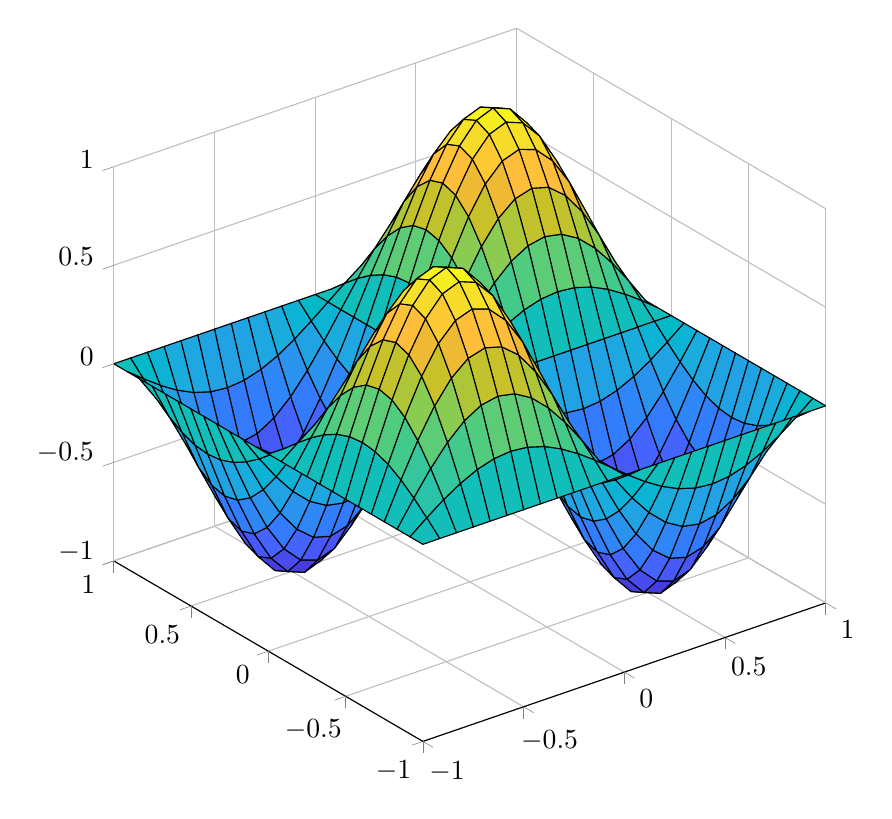
\begin{tikzpicture}

\begin{axis}[%
width=3.56in,
height=3.566in,
at={(0.597in,0.481in)},
scale only axis,
xmin=-1,
xmax=1,
tick align=outside,
ymin=-1,
ymax=1,
zmin=-1,
zmax=1,
view={-37.5}{30},
axis background/.style={fill=white},
axis x line*=bottom,
axis y line*=left,
axis z line*=left,
xmajorgrids,
ymajorgrids,
zmajorgrids,
legend style={at={(1.03,1)}, anchor=north west, legend cell align=left, align=left, draw=white!15!black}
]

\addplot3[%
surf,
shader=flat corner, draw=black, z buffer=sort, colormap={mymap}{[1pt] rgb(0pt)=(0.2422,0.1504,0.6603); rgb(1pt)=(0.25039,0.164995,0.707614); rgb(2pt)=(0.257771,0.181781,0.751138); rgb(3pt)=(0.264729,0.197757,0.795214); rgb(4pt)=(0.270648,0.214676,0.836371); rgb(5pt)=(0.275114,0.234238,0.870986); rgb(6pt)=(0.2783,0.255871,0.899071); rgb(7pt)=(0.280333,0.278233,0.9221); rgb(8pt)=(0.281338,0.300595,0.941376); rgb(9pt)=(0.281014,0.322757,0.957886); rgb(10pt)=(0.279467,0.344671,0.971676); rgb(11pt)=(0.275971,0.366681,0.982905); rgb(12pt)=(0.269914,0.3892,0.9906); rgb(13pt)=(0.260243,0.412329,0.995157); rgb(14pt)=(0.244033,0.435833,0.998833); rgb(15pt)=(0.220643,0.460257,0.997286); rgb(16pt)=(0.196333,0.484719,0.989152); rgb(17pt)=(0.183405,0.507371,0.979795); rgb(18pt)=(0.178643,0.528857,0.968157); rgb(19pt)=(0.176438,0.549905,0.952019); rgb(20pt)=(0.168743,0.570262,0.935871); rgb(21pt)=(0.154,0.5902,0.9218); rgb(22pt)=(0.146029,0.609119,0.907857); rgb(23pt)=(0.138024,0.627629,0.89729); rgb(24pt)=(0.124814,0.645929,0.888343); rgb(25pt)=(0.111252,0.6635,0.876314); rgb(26pt)=(0.0952095,0.679829,0.859781); rgb(27pt)=(0.0688714,0.694771,0.839357); rgb(28pt)=(0.0296667,0.708167,0.816333); rgb(29pt)=(0.00357143,0.720267,0.7917); rgb(30pt)=(0.00665714,0.731214,0.766014); rgb(31pt)=(0.0433286,0.741095,0.73941); rgb(32pt)=(0.0963952,0.75,0.712038); rgb(33pt)=(0.140771,0.7584,0.684157); rgb(34pt)=(0.1717,0.766962,0.655443); rgb(35pt)=(0.193767,0.775767,0.6251); rgb(36pt)=(0.216086,0.7843,0.5923); rgb(37pt)=(0.246957,0.791795,0.556743); rgb(38pt)=(0.290614,0.79729,0.518829); rgb(39pt)=(0.340643,0.8008,0.478857); rgb(40pt)=(0.3909,0.802871,0.435448); rgb(41pt)=(0.445629,0.802419,0.390919); rgb(42pt)=(0.5044,0.7993,0.348); rgb(43pt)=(0.561562,0.794233,0.304481); rgb(44pt)=(0.617395,0.787619,0.261238); rgb(45pt)=(0.671986,0.779271,0.2227); rgb(46pt)=(0.7242,0.769843,0.191029); rgb(47pt)=(0.773833,0.759805,0.16461); rgb(48pt)=(0.820314,0.749814,0.153529); rgb(49pt)=(0.863433,0.7406,0.159633); rgb(50pt)=(0.903543,0.733029,0.177414); rgb(51pt)=(0.939257,0.728786,0.209957); rgb(52pt)=(0.972757,0.729771,0.239443); rgb(53pt)=(0.995648,0.743371,0.237148); rgb(54pt)=(0.996986,0.765857,0.219943); rgb(55pt)=(0.995205,0.789252,0.202762); rgb(56pt)=(0.9892,0.813567,0.188533); rgb(57pt)=(0.978629,0.838629,0.176557); rgb(58pt)=(0.967648,0.8639,0.16429); rgb(59pt)=(0.96101,0.889019,0.153676); rgb(60pt)=(0.959671,0.913457,0.142257); rgb(61pt)=(0.962795,0.937338,0.12651); rgb(62pt)=(0.969114,0.960629,0.106362); rgb(63pt)=(0.9769,0.9839,0.0805)}, mesh/rows=25]
table[row sep=crcr, point meta=\thisrow{c}] {%
%
x	y	z	c\\
-1	-1	1.49975978266186e-32	1.49975978266186e-32\\
-0.916666666666667	-1	0	0\\
-0.833333333333333	-1	6.12323399573676e-17	6.12323399573676e-17\\
-0.75	-1	8.65956056235493e-17	8.65956056235493e-17\\
-0.666666666666667	-1	1.06057523872491e-16	1.06057523872491e-16\\
-0.583333333333333	-1	1.18291797137867e-16	1.18291797137867e-16\\
-0.5	-1	1.22464679914735e-16	1.22464679914735e-16\\
-0.416666666666667	-1	1.18291797137867e-16	1.18291797137867e-16\\
-0.333333333333333	-1	1.06057523872491e-16	1.06057523872491e-16\\
-0.25	-1	8.65956056235493e-17	8.65956056235493e-17\\
-0.166666666666667	-1	6.12323399573676e-17	6.12323399573676e-17\\
-0.0833333333333334	-1	3.16961915143177e-17	3.16961915143177e-17\\
0	-1	-0	-0\\
0.0833333333333333	-1	-3.16961915143176e-17	-3.16961915143176e-17\\
0.166666666666667	-1	-6.12323399573677e-17	-6.12323399573677e-17\\
0.25	-1	-8.65956056235493e-17	-8.65956056235493e-17\\
0.333333333333333	-1	-1.06057523872491e-16	-1.06057523872491e-16\\
0.416666666666667	-1	-1.18291797137867e-16	-1.18291797137867e-16\\
0.5	-1	-1.22464679914735e-16	-1.22464679914735e-16\\
0.583333333333333	-1	-1.18291797137867e-16	-1.18291797137867e-16\\
0.666666666666667	-1	-1.06057523872491e-16	-1.06057523872491e-16\\
0.75	-1	-8.65956056235493e-17	-8.65956056235493e-17\\
0.833333333333333	-1	-6.12323399573677e-17	-6.12323399573677e-17\\
0.916666666666667	-1	-3.16961915143176e-17	-3.16961915143176e-17\\
1	-1	-1.49975978266186e-32	-1.49975978266186e-32\\
-1	-0.916666666666667	3.16961915143177e-17	3.16961915143177e-17\\
-0.916666666666667	-0.916666666666667	0.0669872981077808	0.0669872981077808\\
-0.833333333333333	-0.916666666666667	0.12940952255126	0.12940952255126\\
-0.75	-0.916666666666667	0.18301270189222	0.18301270189222\\
-0.666666666666667	-0.916666666666667	0.224143868042014	0.224143868042014\\
-0.583333333333333	-0.916666666666667	0.25	0.25\\
-0.5	-0.916666666666667	0.258819045102521	0.258819045102521\\
-0.416666666666667	-0.916666666666667	0.25	0.25\\
-0.333333333333333	-0.916666666666667	0.224143868042014	0.224143868042014\\
-0.25	-0.916666666666667	0.183012701892219	0.183012701892219\\
-0.166666666666667	-0.916666666666667	0.12940952255126	0.12940952255126\\
-0.0833333333333334	-0.916666666666667	0.0669872981077808	0.0669872981077808\\
0	-0.916666666666667	-0	-0\\
0.0833333333333333	-0.916666666666667	-0.0669872981077807	-0.0669872981077807\\
0.166666666666667	-0.916666666666667	-0.129409522551261	-0.129409522551261\\
0.25	-0.916666666666667	-0.183012701892219	-0.183012701892219\\
0.333333333333333	-0.916666666666667	-0.224143868042014	-0.224143868042014\\
0.416666666666667	-0.916666666666667	-0.25	-0.25\\
0.5	-0.916666666666667	-0.258819045102521	-0.258819045102521\\
0.583333333333333	-0.916666666666667	-0.25	-0.25\\
0.666666666666667	-0.916666666666667	-0.224143868042014	-0.224143868042014\\
0.75	-0.916666666666667	-0.18301270189222	-0.18301270189222\\
0.833333333333333	-0.916666666666667	-0.129409522551261	-0.129409522551261\\
0.916666666666667	-0.916666666666667	-0.0669872981077807	-0.0669872981077807\\
1	-0.916666666666667	-3.16961915143177e-17	-3.16961915143177e-17\\
-1	-0.833333333333333	6.12323399573676e-17	6.12323399573676e-17\\
-0.916666666666667	-0.833333333333333	0.12940952255126	0.12940952255126\\
-0.833333333333333	-0.833333333333333	0.25	0.25\\
-0.75	-0.833333333333333	0.353553390593274	0.353553390593274\\
-0.666666666666667	-0.833333333333333	0.433012701892219	0.433012701892219\\
-0.583333333333333	-0.833333333333333	0.482962913144534	0.482962913144534\\
-0.5	-0.833333333333333	0.5	0.5\\
-0.416666666666667	-0.833333333333333	0.482962913144534	0.482962913144534\\
-0.333333333333333	-0.833333333333333	0.433012701892219	0.433012701892219\\
-0.25	-0.833333333333333	0.353553390593274	0.353553390593274\\
-0.166666666666667	-0.833333333333333	0.25	0.25\\
-0.0833333333333334	-0.833333333333333	0.12940952255126	0.12940952255126\\
0	-0.833333333333333	-0	-0\\
0.0833333333333333	-0.833333333333333	-0.12940952255126	-0.12940952255126\\
0.166666666666667	-0.833333333333333	-0.25	-0.25\\
0.25	-0.833333333333333	-0.353553390593274	-0.353553390593274\\
0.333333333333333	-0.833333333333333	-0.433012701892219	-0.433012701892219\\
0.416666666666667	-0.833333333333333	-0.482962913144534	-0.482962913144534\\
0.5	-0.833333333333333	-0.5	-0.5\\
0.583333333333333	-0.833333333333333	-0.482962913144534	-0.482962913144534\\
0.666666666666667	-0.833333333333333	-0.433012701892219	-0.433012701892219\\
0.75	-0.833333333333333	-0.353553390593274	-0.353553390593274\\
0.833333333333333	-0.833333333333333	-0.25	-0.25\\
0.916666666666667	-0.833333333333333	-0.12940952255126	-0.12940952255126\\
1	-0.833333333333333	-6.12323399573676e-17	-6.12323399573676e-17\\
-1	-0.75	8.65956056235493e-17	8.65956056235493e-17\\
-0.916666666666667	-0.75	0.18301270189222	0.18301270189222\\
-0.833333333333333	-0.75	0.353553390593274	0.353553390593274\\
-0.75	-0.75	0.5	0.5\\
-0.666666666666667	-0.75	0.612372435695795	0.612372435695795\\
-0.583333333333333	-0.75	0.68301270189222	0.68301270189222\\
-0.5	-0.75	0.707106781186548	0.707106781186548\\
-0.416666666666667	-0.75	0.683012701892219	0.683012701892219\\
-0.333333333333333	-0.75	0.612372435695795	0.612372435695795\\
-0.25	-0.75	0.5	0.5\\
-0.166666666666667	-0.75	0.353553390593274	0.353553390593274\\
-0.0833333333333334	-0.75	0.183012701892219	0.183012701892219\\
0	-0.75	-0	-0\\
0.0833333333333333	-0.75	-0.183012701892219	-0.183012701892219\\
0.166666666666667	-0.75	-0.353553390593274	-0.353553390593274\\
0.25	-0.75	-0.5	-0.5\\
0.333333333333333	-0.75	-0.612372435695794	-0.612372435695794\\
0.416666666666667	-0.75	-0.683012701892219	-0.683012701892219\\
0.5	-0.75	-0.707106781186548	-0.707106781186548\\
0.583333333333333	-0.75	-0.68301270189222	-0.68301270189222\\
0.666666666666667	-0.75	-0.612372435695795	-0.612372435695795\\
0.75	-0.75	-0.5	-0.5\\
0.833333333333333	-0.75	-0.353553390593274	-0.353553390593274\\
0.916666666666667	-0.75	-0.183012701892219	-0.183012701892219\\
1	-0.75	-8.65956056235493e-17	-8.65956056235493e-17\\
-1	-0.666666666666667	1.06057523872491e-16	1.06057523872491e-16\\
-0.916666666666667	-0.666666666666667	0.224143868042014	0.224143868042014\\
-0.833333333333333	-0.666666666666667	0.433012701892219	0.433012701892219\\
-0.75	-0.666666666666667	0.612372435695795	0.612372435695795\\
-0.666666666666667	-0.666666666666667	0.75	0.75\\
-0.583333333333333	-0.666666666666667	0.836516303737808	0.836516303737808\\
-0.5	-0.666666666666667	0.866025403784439	0.866025403784439\\
-0.416666666666667	-0.666666666666667	0.836516303737808	0.836516303737808\\
-0.333333333333333	-0.666666666666667	0.75	0.75\\
-0.25	-0.666666666666667	0.612372435695794	0.612372435695794\\
-0.166666666666667	-0.666666666666667	0.433012701892219	0.433012701892219\\
-0.0833333333333334	-0.666666666666667	0.224143868042013	0.224143868042013\\
0	-0.666666666666667	-0	-0\\
0.0833333333333333	-0.666666666666667	-0.224143868042013	-0.224143868042013\\
0.166666666666667	-0.666666666666667	-0.433012701892219	-0.433012701892219\\
0.25	-0.666666666666667	-0.612372435695794	-0.612372435695794\\
0.333333333333333	-0.666666666666667	-0.75	-0.75\\
0.416666666666667	-0.666666666666667	-0.836516303737808	-0.836516303737808\\
0.5	-0.666666666666667	-0.866025403784439	-0.866025403784439\\
0.583333333333333	-0.666666666666667	-0.836516303737808	-0.836516303737808\\
0.666666666666667	-0.666666666666667	-0.75	-0.75\\
0.75	-0.666666666666667	-0.612372435695795	-0.612372435695795\\
0.833333333333333	-0.666666666666667	-0.43301270189222	-0.43301270189222\\
0.916666666666667	-0.666666666666667	-0.224143868042013	-0.224143868042013\\
1	-0.666666666666667	-1.06057523872491e-16	-1.06057523872491e-16\\
-1	-0.583333333333333	1.18291797137867e-16	1.18291797137867e-16\\
-0.916666666666667	-0.583333333333333	0.25	0.25\\
-0.833333333333333	-0.583333333333333	0.482962913144534	0.482962913144534\\
-0.75	-0.583333333333333	0.68301270189222	0.68301270189222\\
-0.666666666666667	-0.583333333333333	0.836516303737808	0.836516303737808\\
-0.583333333333333	-0.583333333333333	0.93301270189222	0.93301270189222\\
-0.5	-0.583333333333333	0.965925826289068	0.965925826289068\\
-0.416666666666667	-0.583333333333333	0.933012701892219	0.933012701892219\\
-0.333333333333333	-0.583333333333333	0.836516303737808	0.836516303737808\\
-0.25	-0.583333333333333	0.683012701892219	0.683012701892219\\
-0.166666666666667	-0.583333333333333	0.482962913144534	0.482962913144534\\
-0.0833333333333334	-0.583333333333333	0.25	0.25\\
0	-0.583333333333333	-0	-0\\
0.0833333333333333	-0.583333333333333	-0.25	-0.25\\
0.166666666666667	-0.583333333333333	-0.482962913144534	-0.482962913144534\\
0.25	-0.583333333333333	-0.683012701892219	-0.683012701892219\\
0.333333333333333	-0.583333333333333	-0.836516303737808	-0.836516303737808\\
0.416666666666667	-0.583333333333333	-0.93301270189222	-0.93301270189222\\
0.5	-0.583333333333333	-0.965925826289068	-0.965925826289068\\
0.583333333333333	-0.583333333333333	-0.93301270189222	-0.93301270189222\\
0.666666666666667	-0.583333333333333	-0.836516303737808	-0.836516303737808\\
0.75	-0.583333333333333	-0.68301270189222	-0.68301270189222\\
0.833333333333333	-0.583333333333333	-0.482962913144535	-0.482962913144535\\
0.916666666666667	-0.583333333333333	-0.25	-0.25\\
1	-0.583333333333333	-1.18291797137867e-16	-1.18291797137867e-16\\
-1	-0.5	1.22464679914735e-16	1.22464679914735e-16\\
-0.916666666666667	-0.5	0.258819045102521	0.258819045102521\\
-0.833333333333333	-0.5	0.5	0.5\\
-0.75	-0.5	0.707106781186548	0.707106781186548\\
-0.666666666666667	-0.5	0.866025403784439	0.866025403784439\\
-0.583333333333333	-0.5	0.965925826289068	0.965925826289068\\
-0.5	-0.5	1	1\\
-0.416666666666667	-0.5	0.965925826289068	0.965925826289068\\
-0.333333333333333	-0.5	0.866025403784439	0.866025403784439\\
-0.25	-0.5	0.707106781186547	0.707106781186547\\
-0.166666666666667	-0.5	0.5	0.5\\
-0.0833333333333334	-0.5	0.258819045102521	0.258819045102521\\
0	-0.5	-0	-0\\
0.0833333333333333	-0.5	-0.258819045102521	-0.258819045102521\\
0.166666666666667	-0.5	-0.5	-0.5\\
0.25	-0.5	-0.707106781186547	-0.707106781186547\\
0.333333333333333	-0.5	-0.866025403784438	-0.866025403784438\\
0.416666666666667	-0.5	-0.965925826289068	-0.965925826289068\\
0.5	-0.5	-1	-1\\
0.583333333333333	-0.5	-0.965925826289068	-0.965925826289068\\
0.666666666666667	-0.5	-0.866025403784439	-0.866025403784439\\
0.75	-0.5	-0.707106781186548	-0.707106781186548\\
0.833333333333333	-0.5	-0.5	-0.5\\
0.916666666666667	-0.5	-0.258819045102521	-0.258819045102521\\
1	-0.5	-1.22464679914735e-16	-1.22464679914735e-16\\
-1	-0.416666666666667	1.18291797137867e-16	1.18291797137867e-16\\
-0.916666666666667	-0.416666666666667	0.25	0.25\\
-0.833333333333333	-0.416666666666667	0.482962913144534	0.482962913144534\\
-0.75	-0.416666666666667	0.683012701892219	0.683012701892219\\
-0.666666666666667	-0.416666666666667	0.836516303737808	0.836516303737808\\
-0.583333333333333	-0.416666666666667	0.933012701892219	0.933012701892219\\
-0.5	-0.416666666666667	0.965925826289068	0.965925826289068\\
-0.416666666666667	-0.416666666666667	0.933012701892219	0.933012701892219\\
-0.333333333333333	-0.416666666666667	0.836516303737808	0.836516303737808\\
-0.25	-0.416666666666667	0.683012701892219	0.683012701892219\\
-0.166666666666667	-0.416666666666667	0.482962913144534	0.482962913144534\\
-0.0833333333333334	-0.416666666666667	0.25	0.25\\
0	-0.416666666666667	-0	-0\\
0.0833333333333333	-0.416666666666667	-0.25	-0.25\\
0.166666666666667	-0.416666666666667	-0.482962913144534	-0.482962913144534\\
0.25	-0.416666666666667	-0.683012701892219	-0.683012701892219\\
0.333333333333333	-0.416666666666667	-0.836516303737808	-0.836516303737808\\
0.416666666666667	-0.416666666666667	-0.933012701892219	-0.933012701892219\\
0.5	-0.416666666666667	-0.965925826289068	-0.965925826289068\\
0.583333333333333	-0.416666666666667	-0.933012701892219	-0.933012701892219\\
0.666666666666667	-0.416666666666667	-0.836516303737808	-0.836516303737808\\
0.75	-0.416666666666667	-0.683012701892219	-0.683012701892219\\
0.833333333333333	-0.416666666666667	-0.482962913144534	-0.482962913144534\\
0.916666666666667	-0.416666666666667	-0.25	-0.25\\
1	-0.416666666666667	-1.18291797137867e-16	-1.18291797137867e-16\\
-1	-0.333333333333333	1.06057523872491e-16	1.06057523872491e-16\\
-0.916666666666667	-0.333333333333333	0.224143868042014	0.224143868042014\\
-0.833333333333333	-0.333333333333333	0.433012701892219	0.433012701892219\\
-0.75	-0.333333333333333	0.612372435695795	0.612372435695795\\
-0.666666666666667	-0.333333333333333	0.75	0.75\\
-0.583333333333333	-0.333333333333333	0.836516303737808	0.836516303737808\\
-0.5	-0.333333333333333	0.866025403784439	0.866025403784439\\
-0.416666666666667	-0.333333333333333	0.836516303737808	0.836516303737808\\
-0.333333333333333	-0.333333333333333	0.75	0.75\\
-0.25	-0.333333333333333	0.612372435695794	0.612372435695794\\
-0.166666666666667	-0.333333333333333	0.433012701892219	0.433012701892219\\
-0.0833333333333334	-0.333333333333333	0.224143868042013	0.224143868042013\\
0	-0.333333333333333	-0	-0\\
0.0833333333333333	-0.333333333333333	-0.224143868042013	-0.224143868042013\\
0.166666666666667	-0.333333333333333	-0.433012701892219	-0.433012701892219\\
0.25	-0.333333333333333	-0.612372435695794	-0.612372435695794\\
0.333333333333333	-0.333333333333333	-0.75	-0.75\\
0.416666666666667	-0.333333333333333	-0.836516303737808	-0.836516303737808\\
0.5	-0.333333333333333	-0.866025403784439	-0.866025403784439\\
0.583333333333333	-0.333333333333333	-0.836516303737808	-0.836516303737808\\
0.666666666666667	-0.333333333333333	-0.75	-0.75\\
0.75	-0.333333333333333	-0.612372435695795	-0.612372435695795\\
0.833333333333333	-0.333333333333333	-0.43301270189222	-0.43301270189222\\
0.916666666666667	-0.333333333333333	-0.224143868042013	-0.224143868042013\\
1	-0.333333333333333	-1.06057523872491e-16	-1.06057523872491e-16\\
-1	-0.25	8.65956056235493e-17	8.65956056235493e-17\\
-0.916666666666667	-0.25	0.183012701892219	0.183012701892219\\
-0.833333333333333	-0.25	0.353553390593274	0.353553390593274\\
-0.75	-0.25	0.5	0.5\\
-0.666666666666667	-0.25	0.612372435695794	0.612372435695794\\
-0.583333333333333	-0.25	0.683012701892219	0.683012701892219\\
-0.5	-0.25	0.707106781186547	0.707106781186547\\
-0.416666666666667	-0.25	0.683012701892219	0.683012701892219\\
-0.333333333333333	-0.25	0.612372435695794	0.612372435695794\\
-0.25	-0.25	0.5	0.5\\
-0.166666666666667	-0.25	0.353553390593274	0.353553390593274\\
-0.0833333333333334	-0.25	0.183012701892219	0.183012701892219\\
0	-0.25	-0	-0\\
0.0833333333333333	-0.25	-0.183012701892219	-0.183012701892219\\
0.166666666666667	-0.25	-0.353553390593274	-0.353553390593274\\
0.25	-0.25	-0.5	-0.5\\
0.333333333333333	-0.25	-0.612372435695794	-0.612372435695794\\
0.416666666666667	-0.25	-0.683012701892219	-0.683012701892219\\
0.5	-0.25	-0.707106781186547	-0.707106781186547\\
0.583333333333333	-0.25	-0.683012701892219	-0.683012701892219\\
0.666666666666667	-0.25	-0.612372435695794	-0.612372435695794\\
0.75	-0.25	-0.5	-0.5\\
0.833333333333333	-0.25	-0.353553390593274	-0.353553390593274\\
0.916666666666667	-0.25	-0.183012701892219	-0.183012701892219\\
1	-0.25	-8.65956056235493e-17	-8.65956056235493e-17\\
-1	-0.166666666666667	6.12323399573676e-17	6.12323399573676e-17\\
-0.916666666666667	-0.166666666666667	0.12940952255126	0.12940952255126\\
-0.833333333333333	-0.166666666666667	0.25	0.25\\
-0.75	-0.166666666666667	0.353553390593274	0.353553390593274\\
-0.666666666666667	-0.166666666666667	0.433012701892219	0.433012701892219\\
-0.583333333333333	-0.166666666666667	0.482962913144534	0.482962913144534\\
-0.5	-0.166666666666667	0.5	0.5\\
-0.416666666666667	-0.166666666666667	0.482962913144534	0.482962913144534\\
-0.333333333333333	-0.166666666666667	0.433012701892219	0.433012701892219\\
-0.25	-0.166666666666667	0.353553390593274	0.353553390593274\\
-0.166666666666667	-0.166666666666667	0.25	0.25\\
-0.0833333333333334	-0.166666666666667	0.12940952255126	0.12940952255126\\
0	-0.166666666666667	-0	-0\\
0.0833333333333333	-0.166666666666667	-0.12940952255126	-0.12940952255126\\
0.166666666666667	-0.166666666666667	-0.25	-0.25\\
0.25	-0.166666666666667	-0.353553390593274	-0.353553390593274\\
0.333333333333333	-0.166666666666667	-0.433012701892219	-0.433012701892219\\
0.416666666666667	-0.166666666666667	-0.482962913144534	-0.482962913144534\\
0.5	-0.166666666666667	-0.5	-0.5\\
0.583333333333333	-0.166666666666667	-0.482962913144534	-0.482962913144534\\
0.666666666666667	-0.166666666666667	-0.433012701892219	-0.433012701892219\\
0.75	-0.166666666666667	-0.353553390593274	-0.353553390593274\\
0.833333333333333	-0.166666666666667	-0.25	-0.25\\
0.916666666666667	-0.166666666666667	-0.12940952255126	-0.12940952255126\\
1	-0.166666666666667	-6.12323399573676e-17	-6.12323399573676e-17\\
-1	-0.0833333333333334	3.16961915143177e-17	3.16961915143177e-17\\
-0.916666666666667	-0.0833333333333334	0.0669872981077808	0.0669872981077808\\
-0.833333333333333	-0.0833333333333334	0.12940952255126	0.12940952255126\\
-0.75	-0.0833333333333334	0.183012701892219	0.183012701892219\\
-0.666666666666667	-0.0833333333333334	0.224143868042013	0.224143868042013\\
-0.583333333333333	-0.0833333333333334	0.25	0.25\\
-0.5	-0.0833333333333334	0.258819045102521	0.258819045102521\\
-0.416666666666667	-0.0833333333333334	0.25	0.25\\
-0.333333333333333	-0.0833333333333334	0.224143868042013	0.224143868042013\\
-0.25	-0.0833333333333334	0.183012701892219	0.183012701892219\\
-0.166666666666667	-0.0833333333333334	0.12940952255126	0.12940952255126\\
-0.0833333333333334	-0.0833333333333334	0.0669872981077807	0.0669872981077807\\
0	-0.0833333333333334	-0	-0\\
0.0833333333333333	-0.0833333333333334	-0.0669872981077806	-0.0669872981077806\\
0.166666666666667	-0.0833333333333334	-0.12940952255126	-0.12940952255126\\
0.25	-0.0833333333333334	-0.183012701892219	-0.183012701892219\\
0.333333333333333	-0.0833333333333334	-0.224143868042013	-0.224143868042013\\
0.416666666666667	-0.0833333333333334	-0.25	-0.25\\
0.5	-0.0833333333333334	-0.258819045102521	-0.258819045102521\\
0.583333333333333	-0.0833333333333334	-0.25	-0.25\\
0.666666666666667	-0.0833333333333334	-0.224143868042013	-0.224143868042013\\
0.75	-0.0833333333333334	-0.183012701892219	-0.183012701892219\\
0.833333333333333	-0.0833333333333334	-0.129409522551261	-0.129409522551261\\
0.916666666666667	-0.0833333333333334	-0.0669872981077806	-0.0669872981077806\\
1	-0.0833333333333334	-3.16961915143177e-17	-3.16961915143177e-17\\
-1	0	-0	-0\\
-0.916666666666667	0	-0	-0\\
-0.833333333333333	0	-0	-0\\
-0.75	0	-0	-0\\
-0.666666666666667	0	-0	-0\\
-0.583333333333333	0	-0	-0\\
-0.5	0	-0	-0\\
-0.416666666666667	0	-0	-0\\
-0.333333333333333	0	-0	-0\\
-0.25	0	-0	-0\\
-0.166666666666667	0	-0	-0\\
-0.0833333333333334	0	-0	-0\\
0	0	0	0\\
0.0833333333333333	0	0	0\\
0.166666666666667	0	0	0\\
0.25	0	0	0\\
0.333333333333333	0	0	0\\
0.416666666666667	0	0	0\\
0.5	0	0	0\\
0.583333333333333	0	0	0\\
0.666666666666667	0	0	0\\
0.75	0	0	0\\
0.833333333333333	0	0	0\\
0.916666666666667	0	0	0\\
1	0	0	0\\
-1	0.0833333333333333	-3.16961915143176e-17	-3.16961915143176e-17\\
-0.916666666666667	0.0833333333333333	-0.0669872981077807	-0.0669872981077807\\
-0.833333333333333	0.0833333333333333	-0.12940952255126	-0.12940952255126\\
-0.75	0.0833333333333333	-0.183012701892219	-0.183012701892219\\
-0.666666666666667	0.0833333333333333	-0.224143868042013	-0.224143868042013\\
-0.583333333333333	0.0833333333333333	-0.25	-0.25\\
-0.5	0.0833333333333333	-0.258819045102521	-0.258819045102521\\
-0.416666666666667	0.0833333333333333	-0.25	-0.25\\
-0.333333333333333	0.0833333333333333	-0.224143868042013	-0.224143868042013\\
-0.25	0.0833333333333333	-0.183012701892219	-0.183012701892219\\
-0.166666666666667	0.0833333333333333	-0.12940952255126	-0.12940952255126\\
-0.0833333333333334	0.0833333333333333	-0.0669872981077806	-0.0669872981077806\\
0	0.0833333333333333	0	0\\
0.0833333333333333	0.0833333333333333	0.0669872981077805	0.0669872981077805\\
0.166666666666667	0.0833333333333333	0.12940952255126	0.12940952255126\\
0.25	0.0833333333333333	0.183012701892219	0.183012701892219\\
0.333333333333333	0.0833333333333333	0.224143868042013	0.224143868042013\\
0.416666666666667	0.0833333333333333	0.25	0.25\\
0.5	0.0833333333333333	0.258819045102521	0.258819045102521\\
0.583333333333333	0.0833333333333333	0.25	0.25\\
0.666666666666667	0.0833333333333333	0.224143868042013	0.224143868042013\\
0.75	0.0833333333333333	0.183012701892219	0.183012701892219\\
0.833333333333333	0.0833333333333333	0.12940952255126	0.12940952255126\\
0.916666666666667	0.0833333333333333	0.0669872981077806	0.0669872981077806\\
1	0.0833333333333333	3.16961915143176e-17	3.16961915143176e-17\\
-1	0.166666666666667	-6.12323399573677e-17	-6.12323399573677e-17\\
-0.916666666666667	0.166666666666667	-0.129409522551261	-0.129409522551261\\
-0.833333333333333	0.166666666666667	-0.25	-0.25\\
-0.75	0.166666666666667	-0.353553390593274	-0.353553390593274\\
-0.666666666666667	0.166666666666667	-0.433012701892219	-0.433012701892219\\
-0.583333333333333	0.166666666666667	-0.482962913144534	-0.482962913144534\\
-0.5	0.166666666666667	-0.5	-0.5\\
-0.416666666666667	0.166666666666667	-0.482962913144534	-0.482962913144534\\
-0.333333333333333	0.166666666666667	-0.433012701892219	-0.433012701892219\\
-0.25	0.166666666666667	-0.353553390593274	-0.353553390593274\\
-0.166666666666667	0.166666666666667	-0.25	-0.25\\
-0.0833333333333334	0.166666666666667	-0.12940952255126	-0.12940952255126\\
0	0.166666666666667	0	0\\
0.0833333333333333	0.166666666666667	0.12940952255126	0.12940952255126\\
0.166666666666667	0.166666666666667	0.25	0.25\\
0.25	0.166666666666667	0.353553390593274	0.353553390593274\\
0.333333333333333	0.166666666666667	0.433012701892219	0.433012701892219\\
0.416666666666667	0.166666666666667	0.482962913144534	0.482962913144534\\
0.5	0.166666666666667	0.5	0.5\\
0.583333333333333	0.166666666666667	0.482962913144534	0.482962913144534\\
0.666666666666667	0.166666666666667	0.433012701892219	0.433012701892219\\
0.75	0.166666666666667	0.353553390593274	0.353553390593274\\
0.833333333333333	0.166666666666667	0.25	0.25\\
0.916666666666667	0.166666666666667	0.12940952255126	0.12940952255126\\
1	0.166666666666667	6.12323399573677e-17	6.12323399573677e-17\\
-1	0.25	-8.65956056235493e-17	-8.65956056235493e-17\\
-0.916666666666667	0.25	-0.183012701892219	-0.183012701892219\\
-0.833333333333333	0.25	-0.353553390593274	-0.353553390593274\\
-0.75	0.25	-0.5	-0.5\\
-0.666666666666667	0.25	-0.612372435695794	-0.612372435695794\\
-0.583333333333333	0.25	-0.683012701892219	-0.683012701892219\\
-0.5	0.25	-0.707106781186547	-0.707106781186547\\
-0.416666666666667	0.25	-0.683012701892219	-0.683012701892219\\
-0.333333333333333	0.25	-0.612372435695794	-0.612372435695794\\
-0.25	0.25	-0.5	-0.5\\
-0.166666666666667	0.25	-0.353553390593274	-0.353553390593274\\
-0.0833333333333334	0.25	-0.183012701892219	-0.183012701892219\\
0	0.25	0	0\\
0.0833333333333333	0.25	0.183012701892219	0.183012701892219\\
0.166666666666667	0.25	0.353553390593274	0.353553390593274\\
0.25	0.25	0.5	0.5\\
0.333333333333333	0.25	0.612372435695794	0.612372435695794\\
0.416666666666667	0.25	0.683012701892219	0.683012701892219\\
0.5	0.25	0.707106781186547	0.707106781186547\\
0.583333333333333	0.25	0.683012701892219	0.683012701892219\\
0.666666666666667	0.25	0.612372435695794	0.612372435695794\\
0.75	0.25	0.5	0.5\\
0.833333333333333	0.25	0.353553390593274	0.353553390593274\\
0.916666666666667	0.25	0.183012701892219	0.183012701892219\\
1	0.25	8.65956056235493e-17	8.65956056235493e-17\\
-1	0.333333333333333	-1.06057523872491e-16	-1.06057523872491e-16\\
-0.916666666666667	0.333333333333333	-0.224143868042014	-0.224143868042014\\
-0.833333333333333	0.333333333333333	-0.433012701892219	-0.433012701892219\\
-0.75	0.333333333333333	-0.612372435695794	-0.612372435695794\\
-0.666666666666667	0.333333333333333	-0.75	-0.75\\
-0.583333333333333	0.333333333333333	-0.836516303737808	-0.836516303737808\\
-0.5	0.333333333333333	-0.866025403784438	-0.866025403784438\\
-0.416666666666667	0.333333333333333	-0.836516303737808	-0.836516303737808\\
-0.333333333333333	0.333333333333333	-0.75	-0.75\\
-0.25	0.333333333333333	-0.612372435695794	-0.612372435695794\\
-0.166666666666667	0.333333333333333	-0.433012701892219	-0.433012701892219\\
-0.0833333333333334	0.333333333333333	-0.224143868042013	-0.224143868042013\\
0	0.333333333333333	0	0\\
0.0833333333333333	0.333333333333333	0.224143868042013	0.224143868042013\\
0.166666666666667	0.333333333333333	0.433012701892219	0.433012701892219\\
0.25	0.333333333333333	0.612372435695794	0.612372435695794\\
0.333333333333333	0.333333333333333	0.75	0.75\\
0.416666666666667	0.333333333333333	0.836516303737808	0.836516303737808\\
0.5	0.333333333333333	0.866025403784438	0.866025403784438\\
0.583333333333333	0.333333333333333	0.836516303737808	0.836516303737808\\
0.666666666666667	0.333333333333333	0.75	0.75\\
0.75	0.333333333333333	0.612372435695794	0.612372435695794\\
0.833333333333333	0.333333333333333	0.43301270189222	0.43301270189222\\
0.916666666666667	0.333333333333333	0.224143868042013	0.224143868042013\\
1	0.333333333333333	1.06057523872491e-16	1.06057523872491e-16\\
-1	0.416666666666667	-1.18291797137867e-16	-1.18291797137867e-16\\
-0.916666666666667	0.416666666666667	-0.25	-0.25\\
-0.833333333333333	0.416666666666667	-0.482962913144534	-0.482962913144534\\
-0.75	0.416666666666667	-0.683012701892219	-0.683012701892219\\
-0.666666666666667	0.416666666666667	-0.836516303737808	-0.836516303737808\\
-0.583333333333333	0.416666666666667	-0.93301270189222	-0.93301270189222\\
-0.5	0.416666666666667	-0.965925826289068	-0.965925826289068\\
-0.416666666666667	0.416666666666667	-0.933012701892219	-0.933012701892219\\
-0.333333333333333	0.416666666666667	-0.836516303737808	-0.836516303737808\\
-0.25	0.416666666666667	-0.683012701892219	-0.683012701892219\\
-0.166666666666667	0.416666666666667	-0.482962913144534	-0.482962913144534\\
-0.0833333333333334	0.416666666666667	-0.25	-0.25\\
0	0.416666666666667	0	0\\
0.0833333333333333	0.416666666666667	0.25	0.25\\
0.166666666666667	0.416666666666667	0.482962913144534	0.482962913144534\\
0.25	0.416666666666667	0.683012701892219	0.683012701892219\\
0.333333333333333	0.416666666666667	0.836516303737808	0.836516303737808\\
0.416666666666667	0.416666666666667	0.933012701892219	0.933012701892219\\
0.5	0.416666666666667	0.965925826289068	0.965925826289068\\
0.583333333333333	0.416666666666667	0.93301270189222	0.93301270189222\\
0.666666666666667	0.416666666666667	0.836516303737808	0.836516303737808\\
0.75	0.416666666666667	0.683012701892219	0.683012701892219\\
0.833333333333333	0.416666666666667	0.482962913144534	0.482962913144534\\
0.916666666666667	0.416666666666667	0.25	0.25\\
1	0.416666666666667	1.18291797137867e-16	1.18291797137867e-16\\
-1	0.5	-1.22464679914735e-16	-1.22464679914735e-16\\
-0.916666666666667	0.5	-0.258819045102521	-0.258819045102521\\
-0.833333333333333	0.5	-0.5	-0.5\\
-0.75	0.5	-0.707106781186548	-0.707106781186548\\
-0.666666666666667	0.5	-0.866025403784439	-0.866025403784439\\
-0.583333333333333	0.5	-0.965925826289068	-0.965925826289068\\
-0.5	0.5	-1	-1\\
-0.416666666666667	0.5	-0.965925826289068	-0.965925826289068\\
-0.333333333333333	0.5	-0.866025403784439	-0.866025403784439\\
-0.25	0.5	-0.707106781186547	-0.707106781186547\\
-0.166666666666667	0.5	-0.5	-0.5\\
-0.0833333333333334	0.5	-0.258819045102521	-0.258819045102521\\
0	0.5	0	0\\
0.0833333333333333	0.5	0.258819045102521	0.258819045102521\\
0.166666666666667	0.5	0.5	0.5\\
0.25	0.5	0.707106781186547	0.707106781186547\\
0.333333333333333	0.5	0.866025403784438	0.866025403784438\\
0.416666666666667	0.5	0.965925826289068	0.965925826289068\\
0.5	0.5	1	1\\
0.583333333333333	0.5	0.965925826289068	0.965925826289068\\
0.666666666666667	0.5	0.866025403784439	0.866025403784439\\
0.75	0.5	0.707106781186548	0.707106781186548\\
0.833333333333333	0.5	0.5	0.5\\
0.916666666666667	0.5	0.258819045102521	0.258819045102521\\
1	0.5	1.22464679914735e-16	1.22464679914735e-16\\
-1	0.583333333333333	-1.18291797137867e-16	-1.18291797137867e-16\\
-0.916666666666667	0.583333333333333	-0.25	-0.25\\
-0.833333333333333	0.583333333333333	-0.482962913144534	-0.482962913144534\\
-0.75	0.583333333333333	-0.68301270189222	-0.68301270189222\\
-0.666666666666667	0.583333333333333	-0.836516303737808	-0.836516303737808\\
-0.583333333333333	0.583333333333333	-0.93301270189222	-0.93301270189222\\
-0.5	0.583333333333333	-0.965925826289068	-0.965925826289068\\
-0.416666666666667	0.583333333333333	-0.933012701892219	-0.933012701892219\\
-0.333333333333333	0.583333333333333	-0.836516303737808	-0.836516303737808\\
-0.25	0.583333333333333	-0.683012701892219	-0.683012701892219\\
-0.166666666666667	0.583333333333333	-0.482962913144534	-0.482962913144534\\
-0.0833333333333334	0.583333333333333	-0.25	-0.25\\
0	0.583333333333333	0	0\\
0.0833333333333333	0.583333333333333	0.25	0.25\\
0.166666666666667	0.583333333333333	0.482962913144534	0.482962913144534\\
0.25	0.583333333333333	0.683012701892219	0.683012701892219\\
0.333333333333333	0.583333333333333	0.836516303737808	0.836516303737808\\
0.416666666666667	0.583333333333333	0.93301270189222	0.93301270189222\\
0.5	0.583333333333333	0.965925826289068	0.965925826289068\\
0.583333333333333	0.583333333333333	0.93301270189222	0.93301270189222\\
0.666666666666667	0.583333333333333	0.836516303737808	0.836516303737808\\
0.75	0.583333333333333	0.68301270189222	0.68301270189222\\
0.833333333333333	0.583333333333333	0.482962913144535	0.482962913144535\\
0.916666666666667	0.583333333333333	0.25	0.25\\
1	0.583333333333333	1.18291797137867e-16	1.18291797137867e-16\\
-1	0.666666666666667	-1.06057523872491e-16	-1.06057523872491e-16\\
-0.916666666666667	0.666666666666667	-0.224143868042014	-0.224143868042014\\
-0.833333333333333	0.666666666666667	-0.433012701892219	-0.433012701892219\\
-0.75	0.666666666666667	-0.612372435695795	-0.612372435695795\\
-0.666666666666667	0.666666666666667	-0.75	-0.75\\
-0.583333333333333	0.666666666666667	-0.836516303737808	-0.836516303737808\\
-0.5	0.666666666666667	-0.866025403784439	-0.866025403784439\\
-0.416666666666667	0.666666666666667	-0.836516303737808	-0.836516303737808\\
-0.333333333333333	0.666666666666667	-0.75	-0.75\\
-0.25	0.666666666666667	-0.612372435695794	-0.612372435695794\\
-0.166666666666667	0.666666666666667	-0.433012701892219	-0.433012701892219\\
-0.0833333333333334	0.666666666666667	-0.224143868042013	-0.224143868042013\\
0	0.666666666666667	0	0\\
0.0833333333333333	0.666666666666667	0.224143868042013	0.224143868042013\\
0.166666666666667	0.666666666666667	0.433012701892219	0.433012701892219\\
0.25	0.666666666666667	0.612372435695794	0.612372435695794\\
0.333333333333333	0.666666666666667	0.75	0.75\\
0.416666666666667	0.666666666666667	0.836516303737808	0.836516303737808\\
0.5	0.666666666666667	0.866025403784439	0.866025403784439\\
0.583333333333333	0.666666666666667	0.836516303737808	0.836516303737808\\
0.666666666666667	0.666666666666667	0.75	0.75\\
0.75	0.666666666666667	0.612372435695795	0.612372435695795\\
0.833333333333333	0.666666666666667	0.43301270189222	0.43301270189222\\
0.916666666666667	0.666666666666667	0.224143868042013	0.224143868042013\\
1	0.666666666666667	1.06057523872491e-16	1.06057523872491e-16\\
-1	0.75	-8.65956056235493e-17	-8.65956056235493e-17\\
-0.916666666666667	0.75	-0.18301270189222	-0.18301270189222\\
-0.833333333333333	0.75	-0.353553390593274	-0.353553390593274\\
-0.75	0.75	-0.5	-0.5\\
-0.666666666666667	0.75	-0.612372435695795	-0.612372435695795\\
-0.583333333333333	0.75	-0.68301270189222	-0.68301270189222\\
-0.5	0.75	-0.707106781186548	-0.707106781186548\\
-0.416666666666667	0.75	-0.683012701892219	-0.683012701892219\\
-0.333333333333333	0.75	-0.612372435695795	-0.612372435695795\\
-0.25	0.75	-0.5	-0.5\\
-0.166666666666667	0.75	-0.353553390593274	-0.353553390593274\\
-0.0833333333333334	0.75	-0.183012701892219	-0.183012701892219\\
0	0.75	0	0\\
0.0833333333333333	0.75	0.183012701892219	0.183012701892219\\
0.166666666666667	0.75	0.353553390593274	0.353553390593274\\
0.25	0.75	0.5	0.5\\
0.333333333333333	0.75	0.612372435695794	0.612372435695794\\
0.416666666666667	0.75	0.683012701892219	0.683012701892219\\
0.5	0.75	0.707106781186548	0.707106781186548\\
0.583333333333333	0.75	0.68301270189222	0.68301270189222\\
0.666666666666667	0.75	0.612372435695795	0.612372435695795\\
0.75	0.75	0.5	0.5\\
0.833333333333333	0.75	0.353553390593274	0.353553390593274\\
0.916666666666667	0.75	0.183012701892219	0.183012701892219\\
1	0.75	8.65956056235493e-17	8.65956056235493e-17\\
-1	0.833333333333333	0	0\\
-0.916666666666667	0.833333333333333	-0.129409522551261	-0.129409522551261\\
-0.833333333333333	0.833333333333333	-0.25	-0.25\\
-0.75	0.833333333333333	-0.353553390593274	-0.353553390593274\\
-0.666666666666667	0.833333333333333	-0.43301270189222	-0.43301270189222\\
-0.583333333333333	0.833333333333333	-0.482962913144535	-0.482962913144535\\
-0.5	0.833333333333333	-0.5	-0.5\\
-0.416666666666667	0.833333333333333	-0.482962913144534	-0.482962913144534\\
-0.333333333333333	0.833333333333333	-0.43301270189222	-0.43301270189222\\
-0.25	0.833333333333333	-0.353553390593274	-0.353553390593274\\
-0.166666666666667	0.833333333333333	-0.25	-0.25\\
-0.0833333333333334	0.833333333333333	-0.129409522551261	-0.129409522551261\\
0	0.833333333333333	0	0\\
0.0833333333333333	0.833333333333333	0.12940952255126	0.12940952255126\\
0.166666666666667	0.833333333333333	0.25	0.25\\
0.25	0.833333333333333	0.353553390593274	0.353553390593274\\
0.333333333333333	0.833333333333333	0.43301270189222	0.43301270189222\\
0.416666666666667	0.833333333333333	0.482962913144534	0.482962913144534\\
0.5	0.833333333333333	0.5	0.5\\
0.583333333333333	0.833333333333333	0.482962913144535	0.482962913144535\\
0.666666666666667	0.833333333333333	0.43301270189222	0.43301270189222\\
0.75	0.833333333333333	0.353553390593274	0.353553390593274\\
0.833333333333333	0.833333333333333	0.25	0.25\\
0.916666666666667	0.833333333333333	0.12940952255126	0.12940952255126\\
1	0.833333333333333	0	0\\
-1	0.916666666666667	-3.16961915143176e-17	-3.16961915143176e-17\\
-0.916666666666667	0.916666666666667	-0.0669872981077807	-0.0669872981077807\\
-0.833333333333333	0.916666666666667	-0.12940952255126	-0.12940952255126\\
-0.75	0.916666666666667	-0.183012701892219	-0.183012701892219\\
-0.666666666666667	0.916666666666667	-0.224143868042013	-0.224143868042013\\
-0.583333333333333	0.916666666666667	-0.25	-0.25\\
-0.5	0.916666666666667	-0.258819045102521	-0.258819045102521\\
-0.416666666666667	0.916666666666667	-0.25	-0.25\\
-0.333333333333333	0.916666666666667	-0.224143868042013	-0.224143868042013\\
-0.25	0.916666666666667	-0.183012701892219	-0.183012701892219\\
-0.166666666666667	0.916666666666667	-0.12940952255126	-0.12940952255126\\
-0.0833333333333334	0.916666666666667	-0.0669872981077806	-0.0669872981077806\\
0	0.916666666666667	0	0\\
0.0833333333333333	0.916666666666667	0.0669872981077806	0.0669872981077806\\
0.166666666666667	0.916666666666667	0.12940952255126	0.12940952255126\\
0.25	0.916666666666667	0.183012701892219	0.183012701892219\\
0.333333333333333	0.916666666666667	0.224143868042013	0.224143868042013\\
0.416666666666667	0.916666666666667	0.25	0.25\\
0.5	0.916666666666667	0.258819045102521	0.258819045102521\\
0.583333333333333	0.916666666666667	0.25	0.25\\
0.666666666666667	0.916666666666667	0.224143868042013	0.224143868042013\\
0.75	0.916666666666667	0.183012701892219	0.183012701892219\\
0.833333333333333	0.916666666666667	0.12940952255126	0.12940952255126\\
0.916666666666667	0.916666666666667	0.0669872981077806	0.0669872981077806\\
1	0.916666666666667	3.16961915143176e-17	3.16961915143176e-17\\
-1	1	-1.49975978266186e-32	-1.49975978266186e-32\\
-0.916666666666667	1	0	0\\
-0.833333333333333	1	-6.12323399573676e-17	-6.12323399573676e-17\\
-0.75	1	-8.65956056235493e-17	-8.65956056235493e-17\\
-0.666666666666667	1	-1.06057523872491e-16	-1.06057523872491e-16\\
-0.583333333333333	1	-1.18291797137867e-16	-1.18291797137867e-16\\
-0.5	1	-1.22464679914735e-16	-1.22464679914735e-16\\
-0.416666666666667	1	-1.18291797137867e-16	-1.18291797137867e-16\\
-0.333333333333333	1	-1.06057523872491e-16	-1.06057523872491e-16\\
-0.25	1	-8.65956056235493e-17	-8.65956056235493e-17\\
-0.166666666666667	1	-6.12323399573676e-17	-6.12323399573676e-17\\
-0.0833333333333334	1	-3.16961915143177e-17	-3.16961915143177e-17\\
0	1	0	0\\
0.0833333333333333	1	3.16961915143176e-17	3.16961915143176e-17\\
0.166666666666667	1	6.12323399573677e-17	6.12323399573677e-17\\
0.25	1	8.65956056235493e-17	8.65956056235493e-17\\
0.333333333333333	1	1.06057523872491e-16	1.06057523872491e-16\\
0.416666666666667	1	1.18291797137867e-16	1.18291797137867e-16\\
0.5	1	1.22464679914735e-16	1.22464679914735e-16\\
0.583333333333333	1	1.18291797137867e-16	1.18291797137867e-16\\
0.666666666666667	1	1.06057523872491e-16	1.06057523872491e-16\\
0.75	1	8.65956056235493e-17	8.65956056235493e-17\\
0.833333333333333	1	6.12323399573677e-17	6.12323399573677e-17\\
0.916666666666667	1	3.16961915143176e-17	3.16961915143176e-17\\
1	1	1.49975978266186e-32	1.49975978266186e-32\\
};
%\addlegendentry{data1}

\end{axis}
\end{tikzpicture}%
}
\caption{Lösung der ersten \acs{PDE}}
\label{fig:pde1sol}
\end{figure}
\item
Sei $\Omega := B_1(0) = \{x \in \mathbb{R}^2 |\; \|x\|_2 < 1\} \subset \mathbb{R}^2$ und folgende \ac{PDE} gegeben:
\begin{align*}
- \Delta u (x)&= -\exp(-x_1^2 -x_2^2)(-4+4(x_1^2+x_2^2)) && x  \in \Omega\\
u(x) &= 0&& x \in \partial \Omega
\end{align*}
Sie hat die analytische Lösung 
\begin{align*}
u(x) = \exp(-x_1^2-x_2^2) - \frac{1}{e},
\end{align*}  dargestellt in Abbildung \ref{fig:pde2sol}. Wir wählen als Gewichtsfunktion:
\begin{align*}
w(x) = 1 -x_1^2 -x_2^2
\end{align*}
\begin{figure}[ht]
\centering
\resizebox {\columnwidth} {!} {
% This file was created by matlab2tikz.
%
%The latest updates can be retrieved from
%  http://www.mathworks.com/matlabcentral/fileexchange/22022-matlab2tikz-matlab2tikz
%where you can also make suggestions and rate matlab2tikz.
%
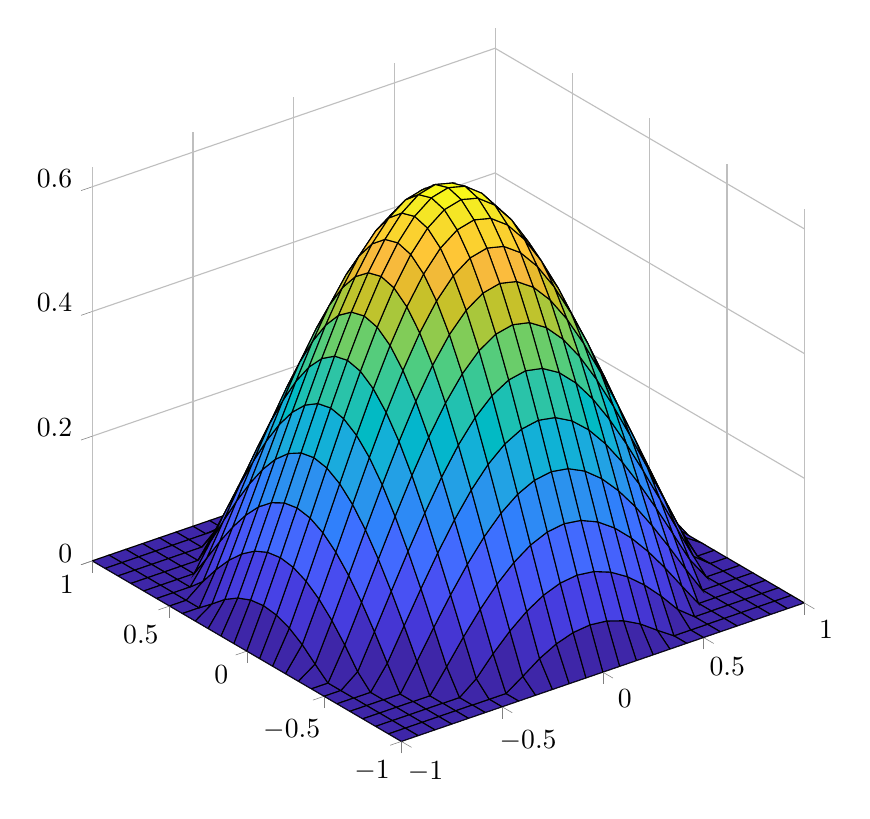
\begin{tikzpicture}

\begin{axis}[%
width=3.56in,
height=3.566in,
at={(0.597in,0.481in)},
scale only axis,
xmin=-1,
xmax=1,
tick align=outside,
ymin=-1,
ymax=1,
zmin=0,
zmax=0.632120558828558,
view={-37.5}{30},
axis background/.style={fill=white},
axis x line*=bottom,
axis y line*=left,
axis z line*=left,
xmajorgrids,
ymajorgrids,
zmajorgrids,
legend style={at={(1.03,1)}, anchor=north west, legend cell align=left, align=left, draw=white!15!black}
]

\addplot3[%
surf,
shader=flat corner, draw=black, z buffer=sort, colormap={mymap}{[1pt] rgb(0pt)=(0.2422,0.1504,0.6603); rgb(1pt)=(0.25039,0.164995,0.707614); rgb(2pt)=(0.257771,0.181781,0.751138); rgb(3pt)=(0.264729,0.197757,0.795214); rgb(4pt)=(0.270648,0.214676,0.836371); rgb(5pt)=(0.275114,0.234238,0.870986); rgb(6pt)=(0.2783,0.255871,0.899071); rgb(7pt)=(0.280333,0.278233,0.9221); rgb(8pt)=(0.281338,0.300595,0.941376); rgb(9pt)=(0.281014,0.322757,0.957886); rgb(10pt)=(0.279467,0.344671,0.971676); rgb(11pt)=(0.275971,0.366681,0.982905); rgb(12pt)=(0.269914,0.3892,0.9906); rgb(13pt)=(0.260243,0.412329,0.995157); rgb(14pt)=(0.244033,0.435833,0.998833); rgb(15pt)=(0.220643,0.460257,0.997286); rgb(16pt)=(0.196333,0.484719,0.989152); rgb(17pt)=(0.183405,0.507371,0.979795); rgb(18pt)=(0.178643,0.528857,0.968157); rgb(19pt)=(0.176438,0.549905,0.952019); rgb(20pt)=(0.168743,0.570262,0.935871); rgb(21pt)=(0.154,0.5902,0.9218); rgb(22pt)=(0.146029,0.609119,0.907857); rgb(23pt)=(0.138024,0.627629,0.89729); rgb(24pt)=(0.124814,0.645929,0.888343); rgb(25pt)=(0.111252,0.6635,0.876314); rgb(26pt)=(0.0952095,0.679829,0.859781); rgb(27pt)=(0.0688714,0.694771,0.839357); rgb(28pt)=(0.0296667,0.708167,0.816333); rgb(29pt)=(0.00357143,0.720267,0.7917); rgb(30pt)=(0.00665714,0.731214,0.766014); rgb(31pt)=(0.0433286,0.741095,0.73941); rgb(32pt)=(0.0963952,0.75,0.712038); rgb(33pt)=(0.140771,0.7584,0.684157); rgb(34pt)=(0.1717,0.766962,0.655443); rgb(35pt)=(0.193767,0.775767,0.6251); rgb(36pt)=(0.216086,0.7843,0.5923); rgb(37pt)=(0.246957,0.791795,0.556743); rgb(38pt)=(0.290614,0.79729,0.518829); rgb(39pt)=(0.340643,0.8008,0.478857); rgb(40pt)=(0.3909,0.802871,0.435448); rgb(41pt)=(0.445629,0.802419,0.390919); rgb(42pt)=(0.5044,0.7993,0.348); rgb(43pt)=(0.561562,0.794233,0.304481); rgb(44pt)=(0.617395,0.787619,0.261238); rgb(45pt)=(0.671986,0.779271,0.2227); rgb(46pt)=(0.7242,0.769843,0.191029); rgb(47pt)=(0.773833,0.759805,0.16461); rgb(48pt)=(0.820314,0.749814,0.153529); rgb(49pt)=(0.863433,0.7406,0.159633); rgb(50pt)=(0.903543,0.733029,0.177414); rgb(51pt)=(0.939257,0.728786,0.209957); rgb(52pt)=(0.972757,0.729771,0.239443); rgb(53pt)=(0.995648,0.743371,0.237148); rgb(54pt)=(0.996986,0.765857,0.219943); rgb(55pt)=(0.995205,0.789252,0.202762); rgb(56pt)=(0.9892,0.813567,0.188533); rgb(57pt)=(0.978629,0.838629,0.176557); rgb(58pt)=(0.967648,0.8639,0.16429); rgb(59pt)=(0.96101,0.889019,0.153676); rgb(60pt)=(0.959671,0.913457,0.142257); rgb(61pt)=(0.962795,0.937338,0.12651); rgb(62pt)=(0.969114,0.960629,0.106362); rgb(63pt)=(0.9769,0.9839,0.0805)}, mesh/rows=25]
table[row sep=crcr, point meta=\thisrow{c}] {%
%
x	y	z	c\\
-1	-1	0	0\\
-0.916666666666667	-1	0	0\\
-0.833333333333333	-1	0	0\\
-0.75	-1	0	0\\
-0.666666666666667	-1	0	0\\
-0.583333333333333	-1	0	0\\
-0.5	-1	0	0\\
-0.416666666666667	-1	0	0\\
-0.333333333333333	-1	0	0\\
-0.25	-1	0	0\\
-0.166666666666667	-1	0	0\\
-0.0833333333333334	-1	0	0\\
0	-1	5.55111512312578e-17	5.55111512312578e-17\\
0.0833333333333333	-1	0	0\\
0.166666666666667	-1	0	0\\
0.25	-1	0	0\\
0.333333333333333	-1	0	0\\
0.416666666666667	-1	0	0\\
0.5	-1	0	0\\
0.583333333333333	-1	0	0\\
0.666666666666667	-1	0	0\\
0.75	-1	0	0\\
0.833333333333333	-1	0	0\\
0.916666666666667	-1	0	0\\
1	-1	0	0\\
-1	-0.916666666666667	0	0\\
-0.916666666666667	-0.916666666666667	0	0\\
-0.833333333333333	-0.916666666666667	0	0\\
-0.75	-0.916666666666667	0	0\\
-0.666666666666667	-0.916666666666667	0	0\\
-0.583333333333333	-0.916666666666667	0	0\\
-0.5	-0.916666666666667	0	0\\
-0.416666666666667	-0.916666666666667	0	0\\
-0.333333333333333	-0.916666666666667	0.0183248148141781	0.0183248148141781\\
-0.25	-0.916666666666667	0.0375624255076384	0.0375624255076384\\
-0.166666666666667	-0.916666666666667	0.0518875286016618	0.0518875286016618\\
-0.0833333333333334	-0.916666666666667	0.0607244049823947	0.0607244049823947\\
0	-0.916666666666667	0.0637111793217526	0.0637111793217526\\
0.0833333333333333	-0.916666666666667	0.0607244049823947	0.0607244049823947\\
0.166666666666667	-0.916666666666667	0.0518875286016618	0.0518875286016618\\
0.25	-0.916666666666667	0.0375624255076384	0.0375624255076384\\
0.333333333333333	-0.916666666666667	0.0183248148141782	0.0183248148141782\\
0.416666666666667	-0.916666666666667	0	0\\
0.5	-0.916666666666667	0	0\\
0.583333333333333	-0.916666666666667	0	0\\
0.666666666666667	-0.916666666666667	0	0\\
0.75	-0.916666666666667	0	0\\
0.833333333333333	-0.916666666666667	0	0\\
0.916666666666667	-0.916666666666667	0	0\\
1	-0.916666666666667	0	0\\
-1	-0.833333333333333	0	0\\
-0.916666666666667	-0.833333333333333	0	0\\
-0.833333333333333	-0.833333333333333	0	0\\
-0.75	-0.833333333333333	0	0\\
-0.666666666666667	-0.833333333333333	0	0\\
-0.583333333333333	-0.833333333333333	0	0\\
-0.5	-0.833333333333333	0.0210161228177806	0.0210161228177806\\
-0.416666666666667	-0.833333333333333	0.0518875286016618	0.0518875286016618\\
-0.333333333333333	-0.833333333333333	0.0789601721887676	0.0789601721887676\\
-0.25	-0.833333333333333	0.101218151977991	0.101218151977991\\
-0.166666666666667	-0.833333333333333	0.11779234407627	0.11779234407627\\
-0.0833333333333334	-0.833333333333333	0.128016639547073	0.128016639547073\\
0	-0.833333333333333	0.131472347427834	0.131472347427834\\
0.0833333333333333	-0.833333333333333	0.128016639547073	0.128016639547073\\
0.166666666666667	-0.833333333333333	0.11779234407627	0.11779234407627\\
0.25	-0.833333333333333	0.101218151977991	0.101218151977991\\
0.333333333333333	-0.833333333333333	0.0789601721887676	0.0789601721887676\\
0.416666666666667	-0.833333333333333	0.0518875286016617	0.0518875286016617\\
0.5	-0.833333333333333	0.0210161228177806	0.0210161228177806\\
0.583333333333333	-0.833333333333333	0	0\\
0.666666666666667	-0.833333333333333	0	0\\
0.75	-0.833333333333333	0	0\\
0.833333333333333	-0.833333333333333	0	0\\
0.916666666666667	-0.833333333333333	0	0\\
1	-0.833333333333333	0	0\\
-1	-0.75	0	0\\
-0.916666666666667	-0.75	0	0\\
-0.833333333333333	-0.75	0	0\\
-0.75	-0.75	0	0\\
-0.666666666666667	-0.75	0	0\\
-0.583333333333333	-0.75	0.0375624255076384	0.0375624255076384\\
-0.5	-0.75	0.0758678689096376	0.0758678689096376\\
-0.416666666666667	-0.75	0.111093529841575	0.111093529841575\\
-0.333333333333333	-0.75	0.141984632443339	0.141984632443339\\
-0.25	-0.75	0.167381987347548	0.167381987347548\\
-0.166666666666667	-0.75	0.186293885145853	0.186293885145853\\
-0.0833333333333334	-0.75	0.19796026561598	0.19796026561598\\
0	-0.75	0.201903383559481	0.201903383559481\\
0.0833333333333333	-0.75	0.19796026561598	0.19796026561598\\
0.166666666666667	-0.75	0.186293885145853	0.186293885145853\\
0.25	-0.75	0.167381987347548	0.167381987347548\\
0.333333333333333	-0.75	0.141984632443339	0.141984632443339\\
0.416666666666667	-0.75	0.111093529841575	0.111093529841575\\
0.5	-0.75	0.0758678689096376	0.0758678689096376\\
0.583333333333333	-0.75	0.0375624255076384	0.0375624255076384\\
0.666666666666667	-0.75	0	0\\
0.75	-0.75	0	0\\
0.833333333333333	-0.75	0	0\\
0.916666666666667	-0.75	0	0\\
1	-0.75	0	0\\
-1	-0.666666666666667	0	0\\
-0.916666666666667	-0.666666666666667	0	0\\
-0.833333333333333	-0.666666666666667	0	0\\
-0.75	-0.666666666666667	0	0\\
-0.666666666666667	-0.666666666666667	0.0432328493357451	0.0432328493357451\\
-0.583333333333333	-0.666666666666667	0.0883669781301998	0.0883669781301998\\
-0.5	-0.666666666666667	0.131472347427834	0.131472347427834\\
-0.416666666666667	-0.666666666666667	0.171112017103218	0.171112017103218\\
-0.333333333333333	-0.666666666666667	0.20587397956599	0.20587397956599\\
-0.25	-0.666666666666667	0.234453791339475	0.234453791339475\\
-0.166666666666667	-0.666666666666667	0.255735475254731	0.255735475254731\\
-0.0833333333333334	-0.666666666666667	0.268863730506967	0.268863730506967\\
0	-0.666666666666667	0.273300947258512	0.273300947258512\\
0.0833333333333333	-0.666666666666667	0.268863730506967	0.268863730506967\\
0.166666666666667	-0.666666666666667	0.255735475254731	0.255735475254731\\
0.25	-0.666666666666667	0.234453791339475	0.234453791339475\\
0.333333333333333	-0.666666666666667	0.20587397956599	0.20587397956599\\
0.416666666666667	-0.666666666666667	0.171112017103218	0.171112017103218\\
0.5	-0.666666666666667	0.131472347427834	0.131472347427834\\
0.583333333333333	-0.666666666666667	0.0883669781301998	0.0883669781301998\\
0.666666666666667	-0.666666666666667	0.0432328493357451	0.0432328493357451\\
0.75	-0.666666666666667	0	0\\
0.833333333333333	-0.666666666666667	0	0\\
0.916666666666667	-0.666666666666667	0	0\\
1	-0.666666666666667	0	0\\
-1	-0.583333333333333	0	0\\
-0.916666666666667	-0.583333333333333	0	0\\
-0.833333333333333	-0.583333333333333	0	0\\
-0.75	-0.583333333333333	0.0375624255076384	0.0375624255076384\\
-0.666666666666667	-0.583333333333333	0.0883669781301998	0.0883669781301998\\
-0.583333333333333	-0.583333333333333	0.138456175476658	0.138456175476658\\
-0.5	-0.583333333333333	0.186293885145853	0.186293885145853\\
-0.416666666666667	-0.583333333333333	0.230285411960539	0.230285411960539\\
-0.333333333333333	-0.583333333333333	0.268863730506967	0.268863730506967\\
-0.25	-0.583333333333333	0.300581188454723	0.300581188454723\\
-0.166666666666667	-0.583333333333333	0.324199290630812	0.324199290630812\\
-0.0833333333333334	-0.583333333333333	0.338768836686274	0.338768836686274\\
0	-0.583333333333333	0.343693195070355	0.343693195070355\\
0.0833333333333333	-0.583333333333333	0.338768836686274	0.338768836686274\\
0.166666666666667	-0.583333333333333	0.324199290630812	0.324199290630812\\
0.25	-0.583333333333333	0.300581188454723	0.300581188454723\\
0.333333333333333	-0.583333333333333	0.268863730506967	0.268863730506967\\
0.416666666666667	-0.583333333333333	0.230285411960539	0.230285411960539\\
0.5	-0.583333333333333	0.186293885145853	0.186293885145853\\
0.583333333333333	-0.583333333333333	0.138456175476658	0.138456175476658\\
0.666666666666667	-0.583333333333333	0.0883669781301998	0.0883669781301998\\
0.75	-0.583333333333333	0.0375624255076384	0.0375624255076384\\
0.833333333333333	-0.583333333333333	0	0\\
0.916666666666667	-0.583333333333333	0	0\\
1	-0.583333333333333	0	0\\
-1	-0.5	0	0\\
-0.916666666666667	-0.5	0	0\\
-0.833333333333333	-0.5	0.0210161228177806	0.0210161228177806\\
-0.75	-0.5	0.0758678689096376	0.0758678689096376\\
-0.666666666666667	-0.5	0.131472347427834	0.131472347427834\\
-0.583333333333333	-0.5	0.186293885145853	0.186293885145853\\
-0.5	-0.5	0.238651218541191	0.238651218541191\\
-0.416666666666667	-0.5	0.286798988405886	0.286798988405886\\
-0.333333333333333	-0.5	0.32902211948667	0.32902211948667\\
-0.25	-0.5	0.3637361877752	0.3637361877752\\
-0.166666666666667	-0.5	0.389585687225524	0.389585687225524\\
-0.0833333333333334	-0.5	0.405531738688263	0.405531738688263\\
0	-0.5	0.410921341899963	0.410921341899963\\
0.0833333333333333	-0.5	0.405531738688263	0.405531738688263\\
0.166666666666667	-0.5	0.389585687225524	0.389585687225524\\
0.25	-0.5	0.3637361877752	0.3637361877752\\
0.333333333333333	-0.5	0.32902211948667	0.32902211948667\\
0.416666666666667	-0.5	0.286798988405886	0.286798988405886\\
0.5	-0.5	0.238651218541191	0.238651218541191\\
0.583333333333333	-0.5	0.186293885145853	0.186293885145853\\
0.666666666666667	-0.5	0.131472347427834	0.131472347427834\\
0.75	-0.5	0.0758678689096376	0.0758678689096376\\
0.833333333333333	-0.5	0.0210161228177807	0.0210161228177807\\
0.916666666666667	-0.5	0	0\\
1	-0.5	0	0\\
-1	-0.416666666666667	0	0\\
-0.916666666666667	-0.416666666666667	0	0\\
-0.833333333333333	-0.416666666666667	0.0518875286016618	0.0518875286016618\\
-0.75	-0.416666666666667	0.111093529841575	0.111093529841575\\
-0.666666666666667	-0.416666666666667	0.171112017103218	0.171112017103218\\
-0.583333333333333	-0.416666666666667	0.230285411960539	0.230285411960539\\
-0.5	-0.416666666666667	0.286798988405886	0.286798988405886\\
-0.416666666666667	-0.416666666666667	0.338768836686274	0.338768836686274\\
-0.333333333333333	-0.416666666666667	0.384343735011945	0.384343735011945\\
-0.25	-0.416666666666667	0.421813484228155	0.421813484228155\\
-0.166666666666667	-0.416666666666667	0.449714975166002	0.449714975166002\\
-0.0833333333333334	-0.416666666666667	0.466926860109347	0.466926860109347\\
0	-0.416666666666667	0.472744302163063	0.472744302163063\\
0.0833333333333333	-0.416666666666667	0.466926860109347	0.466926860109347\\
0.166666666666667	-0.416666666666667	0.449714975166002	0.449714975166002\\
0.25	-0.416666666666667	0.421813484228155	0.421813484228155\\
0.333333333333333	-0.416666666666667	0.384343735011945	0.384343735011945\\
0.416666666666667	-0.416666666666667	0.338768836686274	0.338768836686274\\
0.5	-0.416666666666667	0.286798988405886	0.286798988405886\\
0.583333333333333	-0.416666666666667	0.230285411960539	0.230285411960539\\
0.666666666666667	-0.416666666666667	0.171112017103218	0.171112017103218\\
0.75	-0.416666666666667	0.111093529841575	0.111093529841575\\
0.833333333333333	-0.416666666666667	0.0518875286016619	0.0518875286016619\\
0.916666666666667	-0.416666666666667	0	0\\
1	-0.416666666666667	0	0\\
-1	-0.333333333333333	0	0\\
-0.916666666666667	-0.333333333333333	0.0183248148141781	0.0183248148141781\\
-0.833333333333333	-0.333333333333333	0.0789601721887676	0.0789601721887676\\
-0.75	-0.333333333333333	0.141984632443339	0.141984632443339\\
-0.666666666666667	-0.333333333333333	0.20587397956599	0.20587397956599\\
-0.583333333333333	-0.333333333333333	0.268863730506967	0.268863730506967\\
-0.5	-0.333333333333333	0.32902211948667	0.32902211948667\\
-0.416666666666667	-0.333333333333333	0.384343735011945	0.384343735011945\\
-0.333333333333333	-0.333333333333333	0.432857961745366	0.432857961745366\\
-0.25	-0.333333333333333	0.472744302163063	0.472744302163063\\
-0.166666666666667	-0.333333333333333	0.502445284661948	0.502445284661948\\
-0.0833333333333334	-0.333333333333333	0.520767240811671	0.520767240811671\\
0	-0.333333333333333	0.526959875642927	0.526959875642927\\
0.0833333333333333	-0.333333333333333	0.520767240811671	0.520767240811671\\
0.166666666666667	-0.333333333333333	0.502445284661948	0.502445284661948\\
0.25	-0.333333333333333	0.472744302163063	0.472744302163063\\
0.333333333333333	-0.333333333333333	0.432857961745366	0.432857961745366\\
0.416666666666667	-0.333333333333333	0.384343735011945	0.384343735011945\\
0.5	-0.333333333333333	0.32902211948667	0.32902211948667\\
0.583333333333333	-0.333333333333333	0.268863730506967	0.268863730506967\\
0.666666666666667	-0.333333333333333	0.20587397956599	0.20587397956599\\
0.75	-0.333333333333333	0.141984632443339	0.141984632443339\\
0.833333333333333	-0.333333333333333	0.0789601721887677	0.0789601721887677\\
0.916666666666667	-0.333333333333333	0.018324814814178	0.018324814814178\\
1	-0.333333333333333	0	0\\
-1	-0.25	0	0\\
-0.916666666666667	-0.25	0.0375624255076384	0.0375624255076384\\
-0.833333333333333	-0.25	0.101218151977991	0.101218151977991\\
-0.75	-0.25	0.167381987347548	0.167381987347548\\
-0.666666666666667	-0.25	0.234453791339475	0.234453791339475\\
-0.583333333333333	-0.25	0.300581188454723	0.300581188454723\\
-0.5	-0.25	0.3637361877752	0.3637361877752\\
-0.416666666666667	-0.25	0.421813484228155	0.421813484228155\\
-0.333333333333333	-0.25	0.472744302163063	0.472744302163063\\
-0.25	-0.25	0.514617461413153	0.514617461413153\\
-0.166666666666667	-0.25	0.545797909582526	0.545797909582526\\
-0.0833333333333334	-0.25	0.565032519215705	0.565032519215705\\
0	-0.25	0.571533621642033	0.571533621642033\\
0.0833333333333333	-0.25	0.565032519215705	0.565032519215705\\
0.166666666666667	-0.25	0.545797909582526	0.545797909582526\\
0.25	-0.25	0.514617461413153	0.514617461413153\\
0.333333333333333	-0.25	0.472744302163063	0.472744302163063\\
0.416666666666667	-0.25	0.421813484228155	0.421813484228155\\
0.5	-0.25	0.3637361877752	0.3637361877752\\
0.583333333333333	-0.25	0.300581188454723	0.300581188454723\\
0.666666666666667	-0.25	0.234453791339475	0.234453791339475\\
0.75	-0.25	0.167381987347548	0.167381987347548\\
0.833333333333333	-0.25	0.101218151977991	0.101218151977991\\
0.916666666666667	-0.25	0.0375624255076383	0.0375624255076383\\
1	-0.25	0	0\\
-1	-0.166666666666667	0	0\\
-0.916666666666667	-0.166666666666667	0.0518875286016618	0.0518875286016618\\
-0.833333333333333	-0.166666666666667	0.11779234407627	0.11779234407627\\
-0.75	-0.166666666666667	0.186293885145853	0.186293885145853\\
-0.666666666666667	-0.166666666666667	0.255735475254731	0.255735475254731\\
-0.583333333333333	-0.166666666666667	0.324199290630812	0.324199290630812\\
-0.5	-0.166666666666667	0.389585687225524	0.389585687225524\\
-0.416666666666667	-0.166666666666667	0.449714975166002	0.449714975166002\\
-0.333333333333333	-0.166666666666667	0.502445284661948	0.502445284661948\\
-0.25	-0.166666666666667	0.545797909582526	0.545797909582526\\
-0.166666666666667	-0.166666666666667	0.578080027735323	0.578080027735323\\
-0.0833333333333334	-0.166666666666667	0.597994236069607	0.597994236069607\\
0	-0.166666666666667	0.604725035944906	0.604725035944906\\
0.0833333333333333	-0.166666666666667	0.597994236069607	0.597994236069607\\
0.166666666666667	-0.166666666666667	0.578080027735323	0.578080027735323\\
0.25	-0.166666666666667	0.545797909582526	0.545797909582526\\
0.333333333333333	-0.166666666666667	0.502445284661948	0.502445284661948\\
0.416666666666667	-0.166666666666667	0.449714975166002	0.449714975166002\\
0.5	-0.166666666666667	0.389585687225524	0.389585687225524\\
0.583333333333333	-0.166666666666667	0.324199290630812	0.324199290630812\\
0.666666666666667	-0.166666666666667	0.255735475254731	0.255735475254731\\
0.75	-0.166666666666667	0.186293885145853	0.186293885145853\\
0.833333333333333	-0.166666666666667	0.11779234407627	0.11779234407627\\
0.916666666666667	-0.166666666666667	0.0518875286016617	0.0518875286016617\\
1	-0.166666666666667	0	0\\
-1	-0.0833333333333334	0	0\\
-0.916666666666667	-0.0833333333333334	0.0607244049823947	0.0607244049823947\\
-0.833333333333333	-0.0833333333333334	0.128016639547073	0.128016639547073\\
-0.75	-0.0833333333333334	0.19796026561598	0.19796026561598\\
-0.666666666666667	-0.0833333333333334	0.268863730506967	0.268863730506967\\
-0.583333333333333	-0.0833333333333334	0.338768836686274	0.338768836686274\\
-0.5	-0.0833333333333334	0.405531738688263	0.405531738688263\\
-0.416666666666667	-0.0833333333333334	0.466926860109347	0.466926860109347\\
-0.333333333333333	-0.0833333333333334	0.520767240811671	0.520767240811671\\
-0.25	-0.0833333333333334	0.565032519215705	0.565032519215705\\
-0.166666666666667	-0.0833333333333334	0.597994236069607	0.597994236069607\\
-0.0833333333333334	-0.0833333333333334	0.618327675572474	0.618327675572474\\
0	-0.0833333333333334	0.625200171318874	0.625200171318874\\
0.0833333333333333	-0.0833333333333334	0.618327675572474	0.618327675572474\\
0.166666666666667	-0.0833333333333334	0.597994236069607	0.597994236069607\\
0.25	-0.0833333333333334	0.565032519215705	0.565032519215705\\
0.333333333333333	-0.0833333333333334	0.520767240811671	0.520767240811671\\
0.416666666666667	-0.0833333333333334	0.466926860109347	0.466926860109347\\
0.5	-0.0833333333333334	0.405531738688263	0.405531738688263\\
0.583333333333333	-0.0833333333333334	0.338768836686274	0.338768836686274\\
0.666666666666667	-0.0833333333333334	0.268863730506967	0.268863730506967\\
0.75	-0.0833333333333334	0.19796026561598	0.19796026561598\\
0.833333333333333	-0.0833333333333334	0.128016639547073	0.128016639547073\\
0.916666666666667	-0.0833333333333334	0.0607244049823946	0.0607244049823946\\
1	-0.0833333333333334	0	0\\
-1	0	5.55111512312578e-17	5.55111512312578e-17\\
-0.916666666666667	0	0.0637111793217526	0.0637111793217526\\
-0.833333333333333	0	0.131472347427834	0.131472347427834\\
-0.75	0	0.201903383559481	0.201903383559481\\
-0.666666666666667	0	0.273300947258512	0.273300947258512\\
-0.583333333333333	0	0.343693195070355	0.343693195070355\\
-0.5	0	0.410921341899963	0.410921341899963\\
-0.416666666666667	0	0.472744302163063	0.472744302163063\\
-0.333333333333333	0	0.526959875642927	0.526959875642927\\
-0.25	0	0.571533621642033	0.571533621642033\\
-0.166666666666667	0	0.604725035944906	0.604725035944906\\
-0.0833333333333334	0	0.625200171318874	0.625200171318874\\
0	0	0.632120558828558	0.632120558828558\\
0.0833333333333333	0	0.625200171318874	0.625200171318874\\
0.166666666666667	0	0.604725035944906	0.604725035944906\\
0.25	0	0.571533621642033	0.571533621642033\\
0.333333333333333	0	0.526959875642927	0.526959875642927\\
0.416666666666667	0	0.472744302163063	0.472744302163063\\
0.5	0	0.410921341899963	0.410921341899963\\
0.583333333333333	0	0.343693195070355	0.343693195070355\\
0.666666666666667	0	0.273300947258512	0.273300947258512\\
0.75	0	0.201903383559481	0.201903383559481\\
0.833333333333333	0	0.131472347427834	0.131472347427834\\
0.916666666666667	0	0.0637111793217525	0.0637111793217525\\
1	0	5.55111512312578e-17	5.55111512312578e-17\\
-1	0.0833333333333333	0	0\\
-0.916666666666667	0.0833333333333333	0.0607244049823947	0.0607244049823947\\
-0.833333333333333	0.0833333333333333	0.128016639547073	0.128016639547073\\
-0.75	0.0833333333333333	0.19796026561598	0.19796026561598\\
-0.666666666666667	0.0833333333333333	0.268863730506967	0.268863730506967\\
-0.583333333333333	0.0833333333333333	0.338768836686274	0.338768836686274\\
-0.5	0.0833333333333333	0.405531738688263	0.405531738688263\\
-0.416666666666667	0.0833333333333333	0.466926860109347	0.466926860109347\\
-0.333333333333333	0.0833333333333333	0.520767240811671	0.520767240811671\\
-0.25	0.0833333333333333	0.565032519215705	0.565032519215705\\
-0.166666666666667	0.0833333333333333	0.597994236069607	0.597994236069607\\
-0.0833333333333334	0.0833333333333333	0.618327675572474	0.618327675572474\\
0	0.0833333333333333	0.625200171318874	0.625200171318874\\
0.0833333333333333	0.0833333333333333	0.618327675572474	0.618327675572474\\
0.166666666666667	0.0833333333333333	0.597994236069607	0.597994236069607\\
0.25	0.0833333333333333	0.565032519215705	0.565032519215705\\
0.333333333333333	0.0833333333333333	0.520767240811671	0.520767240811671\\
0.416666666666667	0.0833333333333333	0.466926860109347	0.466926860109347\\
0.5	0.0833333333333333	0.405531738688263	0.405531738688263\\
0.583333333333333	0.0833333333333333	0.338768836686274	0.338768836686274\\
0.666666666666667	0.0833333333333333	0.268863730506967	0.268863730506967\\
0.75	0.0833333333333333	0.19796026561598	0.19796026561598\\
0.833333333333333	0.0833333333333333	0.128016639547073	0.128016639547073\\
0.916666666666667	0.0833333333333333	0.0607244049823946	0.0607244049823946\\
1	0.0833333333333333	0	0\\
-1	0.166666666666667	0	0\\
-0.916666666666667	0.166666666666667	0.0518875286016618	0.0518875286016618\\
-0.833333333333333	0.166666666666667	0.11779234407627	0.11779234407627\\
-0.75	0.166666666666667	0.186293885145853	0.186293885145853\\
-0.666666666666667	0.166666666666667	0.255735475254731	0.255735475254731\\
-0.583333333333333	0.166666666666667	0.324199290630812	0.324199290630812\\
-0.5	0.166666666666667	0.389585687225524	0.389585687225524\\
-0.416666666666667	0.166666666666667	0.449714975166002	0.449714975166002\\
-0.333333333333333	0.166666666666667	0.502445284661948	0.502445284661948\\
-0.25	0.166666666666667	0.545797909582526	0.545797909582526\\
-0.166666666666667	0.166666666666667	0.578080027735323	0.578080027735323\\
-0.0833333333333334	0.166666666666667	0.597994236069607	0.597994236069607\\
0	0.166666666666667	0.604725035944906	0.604725035944906\\
0.0833333333333333	0.166666666666667	0.597994236069607	0.597994236069607\\
0.166666666666667	0.166666666666667	0.578080027735323	0.578080027735323\\
0.25	0.166666666666667	0.545797909582526	0.545797909582526\\
0.333333333333333	0.166666666666667	0.502445284661948	0.502445284661948\\
0.416666666666667	0.166666666666667	0.449714975166002	0.449714975166002\\
0.5	0.166666666666667	0.389585687225524	0.389585687225524\\
0.583333333333333	0.166666666666667	0.324199290630812	0.324199290630812\\
0.666666666666667	0.166666666666667	0.255735475254731	0.255735475254731\\
0.75	0.166666666666667	0.186293885145853	0.186293885145853\\
0.833333333333333	0.166666666666667	0.11779234407627	0.11779234407627\\
0.916666666666667	0.166666666666667	0.0518875286016617	0.0518875286016617\\
1	0.166666666666667	0	0\\
-1	0.25	0	0\\
-0.916666666666667	0.25	0.0375624255076384	0.0375624255076384\\
-0.833333333333333	0.25	0.101218151977991	0.101218151977991\\
-0.75	0.25	0.167381987347548	0.167381987347548\\
-0.666666666666667	0.25	0.234453791339475	0.234453791339475\\
-0.583333333333333	0.25	0.300581188454723	0.300581188454723\\
-0.5	0.25	0.3637361877752	0.3637361877752\\
-0.416666666666667	0.25	0.421813484228155	0.421813484228155\\
-0.333333333333333	0.25	0.472744302163063	0.472744302163063\\
-0.25	0.25	0.514617461413153	0.514617461413153\\
-0.166666666666667	0.25	0.545797909582526	0.545797909582526\\
-0.0833333333333334	0.25	0.565032519215705	0.565032519215705\\
0	0.25	0.571533621642033	0.571533621642033\\
0.0833333333333333	0.25	0.565032519215705	0.565032519215705\\
0.166666666666667	0.25	0.545797909582526	0.545797909582526\\
0.25	0.25	0.514617461413153	0.514617461413153\\
0.333333333333333	0.25	0.472744302163063	0.472744302163063\\
0.416666666666667	0.25	0.421813484228155	0.421813484228155\\
0.5	0.25	0.3637361877752	0.3637361877752\\
0.583333333333333	0.25	0.300581188454723	0.300581188454723\\
0.666666666666667	0.25	0.234453791339475	0.234453791339475\\
0.75	0.25	0.167381987347548	0.167381987347548\\
0.833333333333333	0.25	0.101218151977991	0.101218151977991\\
0.916666666666667	0.25	0.0375624255076383	0.0375624255076383\\
1	0.25	0	0\\
-1	0.333333333333333	0	0\\
-0.916666666666667	0.333333333333333	0.0183248148141782	0.0183248148141782\\
-0.833333333333333	0.333333333333333	0.0789601721887676	0.0789601721887676\\
-0.75	0.333333333333333	0.141984632443339	0.141984632443339\\
-0.666666666666667	0.333333333333333	0.20587397956599	0.20587397956599\\
-0.583333333333333	0.333333333333333	0.268863730506967	0.268863730506967\\
-0.5	0.333333333333333	0.32902211948667	0.32902211948667\\
-0.416666666666667	0.333333333333333	0.384343735011945	0.384343735011945\\
-0.333333333333333	0.333333333333333	0.432857961745366	0.432857961745366\\
-0.25	0.333333333333333	0.472744302163063	0.472744302163063\\
-0.166666666666667	0.333333333333333	0.502445284661948	0.502445284661948\\
-0.0833333333333334	0.333333333333333	0.520767240811671	0.520767240811671\\
0	0.333333333333333	0.526959875642927	0.526959875642927\\
0.0833333333333333	0.333333333333333	0.520767240811671	0.520767240811671\\
0.166666666666667	0.333333333333333	0.502445284661948	0.502445284661948\\
0.25	0.333333333333333	0.472744302163063	0.472744302163063\\
0.333333333333333	0.333333333333333	0.432857961745366	0.432857961745366\\
0.416666666666667	0.333333333333333	0.384343735011945	0.384343735011945\\
0.5	0.333333333333333	0.32902211948667	0.32902211948667\\
0.583333333333333	0.333333333333333	0.268863730506967	0.268863730506967\\
0.666666666666667	0.333333333333333	0.20587397956599	0.20587397956599\\
0.75	0.333333333333333	0.141984632443339	0.141984632443339\\
0.833333333333333	0.333333333333333	0.0789601721887677	0.0789601721887677\\
0.916666666666667	0.333333333333333	0.0183248148141781	0.0183248148141781\\
1	0.333333333333333	0	0\\
-1	0.416666666666667	0	0\\
-0.916666666666667	0.416666666666667	0	0\\
-0.833333333333333	0.416666666666667	0.0518875286016617	0.0518875286016617\\
-0.75	0.416666666666667	0.111093529841575	0.111093529841575\\
-0.666666666666667	0.416666666666667	0.171112017103218	0.171112017103218\\
-0.583333333333333	0.416666666666667	0.230285411960539	0.230285411960539\\
-0.5	0.416666666666667	0.286798988405886	0.286798988405886\\
-0.416666666666667	0.416666666666667	0.338768836686274	0.338768836686274\\
-0.333333333333333	0.416666666666667	0.384343735011945	0.384343735011945\\
-0.25	0.416666666666667	0.421813484228155	0.421813484228155\\
-0.166666666666667	0.416666666666667	0.449714975166002	0.449714975166002\\
-0.0833333333333334	0.416666666666667	0.466926860109347	0.466926860109347\\
0	0.416666666666667	0.472744302163063	0.472744302163063\\
0.0833333333333333	0.416666666666667	0.466926860109347	0.466926860109347\\
0.166666666666667	0.416666666666667	0.449714975166002	0.449714975166002\\
0.25	0.416666666666667	0.421813484228155	0.421813484228155\\
0.333333333333333	0.416666666666667	0.384343735011945	0.384343735011945\\
0.416666666666667	0.416666666666667	0.338768836686274	0.338768836686274\\
0.5	0.416666666666667	0.286798988405886	0.286798988405886\\
0.583333333333333	0.416666666666667	0.230285411960539	0.230285411960539\\
0.666666666666667	0.416666666666667	0.171112017103218	0.171112017103218\\
0.75	0.416666666666667	0.111093529841575	0.111093529841575\\
0.833333333333333	0.416666666666667	0.0518875286016618	0.0518875286016618\\
0.916666666666667	0.416666666666667	0	0\\
1	0.416666666666667	0	0\\
-1	0.5	0	0\\
-0.916666666666667	0.5	0	0\\
-0.833333333333333	0.5	0.0210161228177806	0.0210161228177806\\
-0.75	0.5	0.0758678689096376	0.0758678689096376\\
-0.666666666666667	0.5	0.131472347427834	0.131472347427834\\
-0.583333333333333	0.5	0.186293885145853	0.186293885145853\\
-0.5	0.5	0.238651218541191	0.238651218541191\\
-0.416666666666667	0.5	0.286798988405886	0.286798988405886\\
-0.333333333333333	0.5	0.32902211948667	0.32902211948667\\
-0.25	0.5	0.3637361877752	0.3637361877752\\
-0.166666666666667	0.5	0.389585687225524	0.389585687225524\\
-0.0833333333333334	0.5	0.405531738688263	0.405531738688263\\
0	0.5	0.410921341899963	0.410921341899963\\
0.0833333333333333	0.5	0.405531738688263	0.405531738688263\\
0.166666666666667	0.5	0.389585687225524	0.389585687225524\\
0.25	0.5	0.3637361877752	0.3637361877752\\
0.333333333333333	0.5	0.32902211948667	0.32902211948667\\
0.416666666666667	0.5	0.286798988405886	0.286798988405886\\
0.5	0.5	0.238651218541191	0.238651218541191\\
0.583333333333333	0.5	0.186293885145853	0.186293885145853\\
0.666666666666667	0.5	0.131472347427834	0.131472347427834\\
0.75	0.5	0.0758678689096376	0.0758678689096376\\
0.833333333333333	0.5	0.0210161228177807	0.0210161228177807\\
0.916666666666667	0.5	0	0\\
1	0.5	0	0\\
-1	0.583333333333333	0	0\\
-0.916666666666667	0.583333333333333	0	0\\
-0.833333333333333	0.583333333333333	0	0\\
-0.75	0.583333333333333	0.0375624255076384	0.0375624255076384\\
-0.666666666666667	0.583333333333333	0.0883669781301998	0.0883669781301998\\
-0.583333333333333	0.583333333333333	0.138456175476658	0.138456175476658\\
-0.5	0.583333333333333	0.186293885145853	0.186293885145853\\
-0.416666666666667	0.583333333333333	0.230285411960539	0.230285411960539\\
-0.333333333333333	0.583333333333333	0.268863730506967	0.268863730506967\\
-0.25	0.583333333333333	0.300581188454723	0.300581188454723\\
-0.166666666666667	0.583333333333333	0.324199290630812	0.324199290630812\\
-0.0833333333333334	0.583333333333333	0.338768836686274	0.338768836686274\\
0	0.583333333333333	0.343693195070355	0.343693195070355\\
0.0833333333333333	0.583333333333333	0.338768836686274	0.338768836686274\\
0.166666666666667	0.583333333333333	0.324199290630812	0.324199290630812\\
0.25	0.583333333333333	0.300581188454723	0.300581188454723\\
0.333333333333333	0.583333333333333	0.268863730506967	0.268863730506967\\
0.416666666666667	0.583333333333333	0.230285411960539	0.230285411960539\\
0.5	0.583333333333333	0.186293885145853	0.186293885145853\\
0.583333333333333	0.583333333333333	0.138456175476658	0.138456175476658\\
0.666666666666667	0.583333333333333	0.0883669781301998	0.0883669781301998\\
0.75	0.583333333333333	0.0375624255076384	0.0375624255076384\\
0.833333333333333	0.583333333333333	0	0\\
0.916666666666667	0.583333333333333	0	0\\
1	0.583333333333333	0	0\\
-1	0.666666666666667	0	0\\
-0.916666666666667	0.666666666666667	0	0\\
-0.833333333333333	0.666666666666667	0	0\\
-0.75	0.666666666666667	0	0\\
-0.666666666666667	0.666666666666667	0.0432328493357451	0.0432328493357451\\
-0.583333333333333	0.666666666666667	0.0883669781301998	0.0883669781301998\\
-0.5	0.666666666666667	0.131472347427834	0.131472347427834\\
-0.416666666666667	0.666666666666667	0.171112017103218	0.171112017103218\\
-0.333333333333333	0.666666666666667	0.20587397956599	0.20587397956599\\
-0.25	0.666666666666667	0.234453791339475	0.234453791339475\\
-0.166666666666667	0.666666666666667	0.255735475254731	0.255735475254731\\
-0.0833333333333334	0.666666666666667	0.268863730506967	0.268863730506967\\
0	0.666666666666667	0.273300947258512	0.273300947258512\\
0.0833333333333333	0.666666666666667	0.268863730506967	0.268863730506967\\
0.166666666666667	0.666666666666667	0.255735475254731	0.255735475254731\\
0.25	0.666666666666667	0.234453791339475	0.234453791339475\\
0.333333333333333	0.666666666666667	0.20587397956599	0.20587397956599\\
0.416666666666667	0.666666666666667	0.171112017103218	0.171112017103218\\
0.5	0.666666666666667	0.131472347427834	0.131472347427834\\
0.583333333333333	0.666666666666667	0.0883669781301998	0.0883669781301998\\
0.666666666666667	0.666666666666667	0.0432328493357451	0.0432328493357451\\
0.75	0.666666666666667	0	0\\
0.833333333333333	0.666666666666667	0	0\\
0.916666666666667	0.666666666666667	0	0\\
1	0.666666666666667	0	0\\
-1	0.75	0	0\\
-0.916666666666667	0.75	0	0\\
-0.833333333333333	0.75	0	0\\
-0.75	0.75	0	0\\
-0.666666666666667	0.75	0	0\\
-0.583333333333333	0.75	0.0375624255076384	0.0375624255076384\\
-0.5	0.75	0.0758678689096376	0.0758678689096376\\
-0.416666666666667	0.75	0.111093529841575	0.111093529841575\\
-0.333333333333333	0.75	0.141984632443339	0.141984632443339\\
-0.25	0.75	0.167381987347548	0.167381987347548\\
-0.166666666666667	0.75	0.186293885145853	0.186293885145853\\
-0.0833333333333334	0.75	0.19796026561598	0.19796026561598\\
0	0.75	0.201903383559481	0.201903383559481\\
0.0833333333333333	0.75	0.19796026561598	0.19796026561598\\
0.166666666666667	0.75	0.186293885145853	0.186293885145853\\
0.25	0.75	0.167381987347548	0.167381987347548\\
0.333333333333333	0.75	0.141984632443339	0.141984632443339\\
0.416666666666667	0.75	0.111093529841575	0.111093529841575\\
0.5	0.75	0.0758678689096376	0.0758678689096376\\
0.583333333333333	0.75	0.0375624255076384	0.0375624255076384\\
0.666666666666667	0.75	0	0\\
0.75	0.75	0	0\\
0.833333333333333	0.75	0	0\\
0.916666666666667	0.75	0	0\\
1	0.75	0	0\\
-1	0.833333333333333	0	0\\
-0.916666666666667	0.833333333333333	0	0\\
-0.833333333333333	0.833333333333333	0	0\\
-0.75	0.833333333333333	0	0\\
-0.666666666666667	0.833333333333333	0	0\\
-0.583333333333333	0.833333333333333	0	0\\
-0.5	0.833333333333333	0.0210161228177807	0.0210161228177807\\
-0.416666666666667	0.833333333333333	0.0518875286016619	0.0518875286016619\\
-0.333333333333333	0.833333333333333	0.0789601721887677	0.0789601721887677\\
-0.25	0.833333333333333	0.101218151977991	0.101218151977991\\
-0.166666666666667	0.833333333333333	0.11779234407627	0.11779234407627\\
-0.0833333333333334	0.833333333333333	0.128016639547073	0.128016639547073\\
0	0.833333333333333	0.131472347427834	0.131472347427834\\
0.0833333333333333	0.833333333333333	0.128016639547073	0.128016639547073\\
0.166666666666667	0.833333333333333	0.11779234407627	0.11779234407627\\
0.25	0.833333333333333	0.101218151977991	0.101218151977991\\
0.333333333333333	0.833333333333333	0.0789601721887677	0.0789601721887677\\
0.416666666666667	0.833333333333333	0.0518875286016618	0.0518875286016618\\
0.5	0.833333333333333	0.0210161228177807	0.0210161228177807\\
0.583333333333333	0.833333333333333	0	0\\
0.666666666666667	0.833333333333333	0	0\\
0.75	0.833333333333333	0	0\\
0.833333333333333	0.833333333333333	0	0\\
0.916666666666667	0.833333333333333	0	0\\
1	0.833333333333333	0	0\\
-1	0.916666666666667	0	0\\
-0.916666666666667	0.916666666666667	0	0\\
-0.833333333333333	0.916666666666667	0	0\\
-0.75	0.916666666666667	0	0\\
-0.666666666666667	0.916666666666667	0	0\\
-0.583333333333333	0.916666666666667	0	0\\
-0.5	0.916666666666667	0	0\\
-0.416666666666667	0.916666666666667	0	0\\
-0.333333333333333	0.916666666666667	0.018324814814178	0.018324814814178\\
-0.25	0.916666666666667	0.0375624255076383	0.0375624255076383\\
-0.166666666666667	0.916666666666667	0.0518875286016617	0.0518875286016617\\
-0.0833333333333334	0.916666666666667	0.0607244049823946	0.0607244049823946\\
0	0.916666666666667	0.0637111793217525	0.0637111793217525\\
0.0833333333333333	0.916666666666667	0.0607244049823946	0.0607244049823946\\
0.166666666666667	0.916666666666667	0.0518875286016617	0.0518875286016617\\
0.25	0.916666666666667	0.0375624255076383	0.0375624255076383\\
0.333333333333333	0.916666666666667	0.0183248148141781	0.0183248148141781\\
0.416666666666667	0.916666666666667	0	0\\
0.5	0.916666666666667	0	0\\
0.583333333333333	0.916666666666667	0	0\\
0.666666666666667	0.916666666666667	0	0\\
0.75	0.916666666666667	0	0\\
0.833333333333333	0.916666666666667	0	0\\
0.916666666666667	0.916666666666667	0	0\\
1	0.916666666666667	0	0\\
-1	1	0	0\\
-0.916666666666667	1	0	0\\
-0.833333333333333	1	0	0\\
-0.75	1	0	0\\
-0.666666666666667	1	0	0\\
-0.583333333333333	1	0	0\\
-0.5	1	0	0\\
-0.416666666666667	1	0	0\\
-0.333333333333333	1	0	0\\
-0.25	1	0	0\\
-0.166666666666667	1	0	0\\
-0.0833333333333334	1	0	0\\
0	1	5.55111512312578e-17	5.55111512312578e-17\\
0.0833333333333333	1	0	0\\
0.166666666666667	1	0	0\\
0.25	1	0	0\\
0.333333333333333	1	0	0\\
0.416666666666667	1	0	0\\
0.5	1	0	0\\
0.583333333333333	1	0	0\\
0.666666666666667	1	0	0\\
0.75	1	0	0\\
0.833333333333333	1	0	0\\
0.916666666666667	1	0	0\\
1	1	0	0\\
};
%\addlegendentry{data1}

\end{axis}
\end{tikzpicture}%
}
\caption{Lösung der zweiten \acs{PDE}}
\label{fig:pde2sol}
\end{figure}
\end{enumerate}


Die Poisson-Gleichung werden wir mithilfe der Kernkollokation numerisch lösen. Dafür wählen wir den Gauß Kern aus Beispiel \ref{ex:Kern}. Im Anhang (Abbildung \ref{fig:wendland-error-grid-both}, \ref{fig:wendland-error-greedy-both}) findet man die den hier nachfolgenden Fehlerplots entsprechenden Plots für einen leicht veränderten $C^4$ Wendland Kern (zu finden in \textcite[Kapitel 9.4]{Wendland.2005}). Dabei haben wir die $\|x-y\|$ Terme quadriert, um Nullstellen im Nenner der partiellen Ableitungen zu vermeiden. Dieser Kern hat aufgrund numerischer Ungenauigkeiten entweder schlechtere oder komplett unbrauchbare Ergebnisse geliefert, weswegen wir ihn nicht genauer betrachten werden. Ebenso werden wir den absoluten Fehlerschätzer, wie in Kapitel \ref{cha:Implementierung} vorgestellt, als Methode zur Fehlerberechnung in jeder Iteration nicht betrachten, sondern nur die im Residuum. Auch hierfür findet man im Anhang (Abbildung \ref{fig:abs-error-grid-both}, \ref{fig:abs-error-greedy-both}) die entsprechenden Plots. Diese weisen allerdings keinen nennenswerten Unterschied zu dem Fehlerschätzer im Residuum auf.

\section{Fehler}

Als Maß des Fehlers unserer numerischen Lösung wollen wir den maximalen absoluten Fehler zur analytischen Lösung berechnen, also
\begin{align*}
\text{error} = \max_{x \in \Omega} |u(x) - s_u (x)|,
\end{align*}
wobei $s_u$ die numerische Lösung bezeichnet. Um den Fehler näherungsweise zu bestimmen, legen wir ein eng gewähltes Gitter an Testpunkten über $\Omega$ und bestimmen ihn an diesen Punkten.
\subsection{Fehler im Inneren}

Wir werden die drei in Kapitel \ref{cha:Implementierung} vorgestellten Methoden zur Kollokationspunktwahl testen und miteinander vergleichen. 

\subsubsection{Kollokationspunkte als Gitter}
Wir werden die Kollokationspunkte, so wie die Validationspunkte, zunächst, wie in Abbildung \ref{fig:Kollok} gezeigt, in einem Gitter anordnen.
\begin{figure}[H]
\centering
\resizebox {.6\columnwidth} {!} {
% This file was created by matlab2tikz.
%
%The latest updates can be retrieved from
%  http://www.mathworks.com/matlabcentral/fileexchange/22022-matlab2tikz-matlab2tikz
%where you can also make suggestions and rate matlab2tikz.
%
\definecolor{mycolor1}{rgb}{0.00000,0.44700,0.74100}%
%
\begin{tikzpicture}

\begin{axis}[%
width=4.in,
height=4.in,
at={(0.983in,0.681in)},
scale only axis,
xmin=-1,
xmax=1,
ymin=-1,
ymax=1,
axis background/.style={fill=white},
axis x line*=bottom,
axis y line*=left,
legend style={legend cell align=left, align=left, draw=white!15!black}
]
\addplot [color=red, draw=none, mark=+, mark options={solid, red}]
  table[row sep=crcr]{%
-0.777777777777778	-0.777777777777778\\
-0.555555555555556	-0.777777777777778\\
-0.333333333333333	-0.777777777777778\\
-0.111111111111111	-0.777777777777778\\
0.111111111111111	-0.777777777777778\\
0.333333333333333	-0.777777777777778\\
0.555555555555556	-0.777777777777778\\
0.777777777777778	-0.777777777777778\\
-0.777777777777778	-0.555555555555556\\
-0.555555555555556	-0.555555555555556\\
-0.333333333333333	-0.555555555555556\\
-0.111111111111111	-0.555555555555556\\
0.111111111111111	-0.555555555555556\\
0.333333333333333	-0.555555555555556\\
0.555555555555556	-0.555555555555556\\
0.777777777777778	-0.555555555555556\\
-0.777777777777778	-0.333333333333333\\
-0.555555555555556	-0.333333333333333\\
-0.333333333333333	-0.333333333333333\\
-0.111111111111111	-0.333333333333333\\
0.111111111111111	-0.333333333333333\\
0.333333333333333	-0.333333333333333\\
0.555555555555556	-0.333333333333333\\
0.777777777777778	-0.333333333333333\\
-0.777777777777778	-0.111111111111111\\
-0.555555555555556	-0.111111111111111\\
-0.333333333333333	-0.111111111111111\\
-0.111111111111111	-0.111111111111111\\
0.111111111111111	-0.111111111111111\\
0.333333333333333	-0.111111111111111\\
0.555555555555556	-0.111111111111111\\
0.777777777777778	-0.111111111111111\\
-0.777777777777778	0.111111111111111\\
-0.555555555555556	0.111111111111111\\
-0.333333333333333	0.111111111111111\\
-0.111111111111111	0.111111111111111\\
0.111111111111111	0.111111111111111\\
0.333333333333333	0.111111111111111\\
0.555555555555556	0.111111111111111\\
0.777777777777778	0.111111111111111\\
-0.777777777777778	0.333333333333333\\
-0.555555555555556	0.333333333333333\\
-0.333333333333333	0.333333333333333\\
-0.111111111111111	0.333333333333333\\
0.111111111111111	0.333333333333333\\
0.333333333333333	0.333333333333333\\
0.555555555555556	0.333333333333333\\
0.777777777777778	0.333333333333333\\
-0.777777777777778	0.555555555555556\\
-0.555555555555556	0.555555555555556\\
-0.333333333333333	0.555555555555556\\
-0.111111111111111	0.555555555555556\\
0.111111111111111	0.555555555555556\\
0.333333333333333	0.555555555555556\\
0.555555555555556	0.555555555555556\\
0.777777777777778	0.555555555555556\\
-0.777777777777778	0.777777777777778\\
-0.555555555555556	0.777777777777778\\
-0.333333333333333	0.777777777777778\\
-0.111111111111111	0.777777777777778\\
0.111111111111111	0.777777777777778\\
0.333333333333333	0.777777777777778\\
0.555555555555556	0.777777777777778\\
0.777777777777778	0.777777777777778\\
};
\addlegendentry{Kollokationspunkte}

\addplot [color=blue, draw=none, mark=asterisk, mark options={solid, blue}]
  table[row sep=crcr]{%
-0.5	-0.5\\
0	-0.5\\
0.5	-0.5\\
-0.5	0\\
0	0\\
0.5	0\\
-0.5	0.5\\
0	0.5\\
0.5	0.5\\
};
\addlegendentry{Testpunkte}

\addplot [color=mycolor1, forget plot]
  table[row sep=crcr]{%
-1	-1\\
-1	1\\
1	1\\
1	-1\\
-1	-1\\
};
\end{axis}
\end{tikzpicture}%
}
\caption{Kollokations- und Validationspunkte auf einem Gitter}
\label{fig:Kollok}
\end{figure}

Damit können wir uns anschauen, wie sich der Fehler bei Verfeinerung des Gitters verhält. Dieser ist in Abbildung \ref{fig:error-grid-both} für die vier verschiedenen Verfahren und beide \acp{PDE} dargestellt. 
%\begin{figure}[ht]
%\centering
%\resizebox {\columnwidth} {!} {
%% This file was created by matlab2tikz.
%
%The latest updates can be retrieved from
%  http://www.mathworks.com/matlabcentral/fileexchange/22022-matlab2tikz-matlab2tikz
%where you can also make suggestions and rate matlab2tikz.
%
\definecolor{mycolor1}{rgb}{0.00000,0.44700,0.74100}%
\definecolor{mycolor2}{rgb}{0.85000,0.32500,0.09800}%
\definecolor{mycolor3}{rgb}{0.92900,0.69400,0.12500}%
\definecolor{mycolor4}{rgb}{0.49400,0.18400,0.55600}%
%
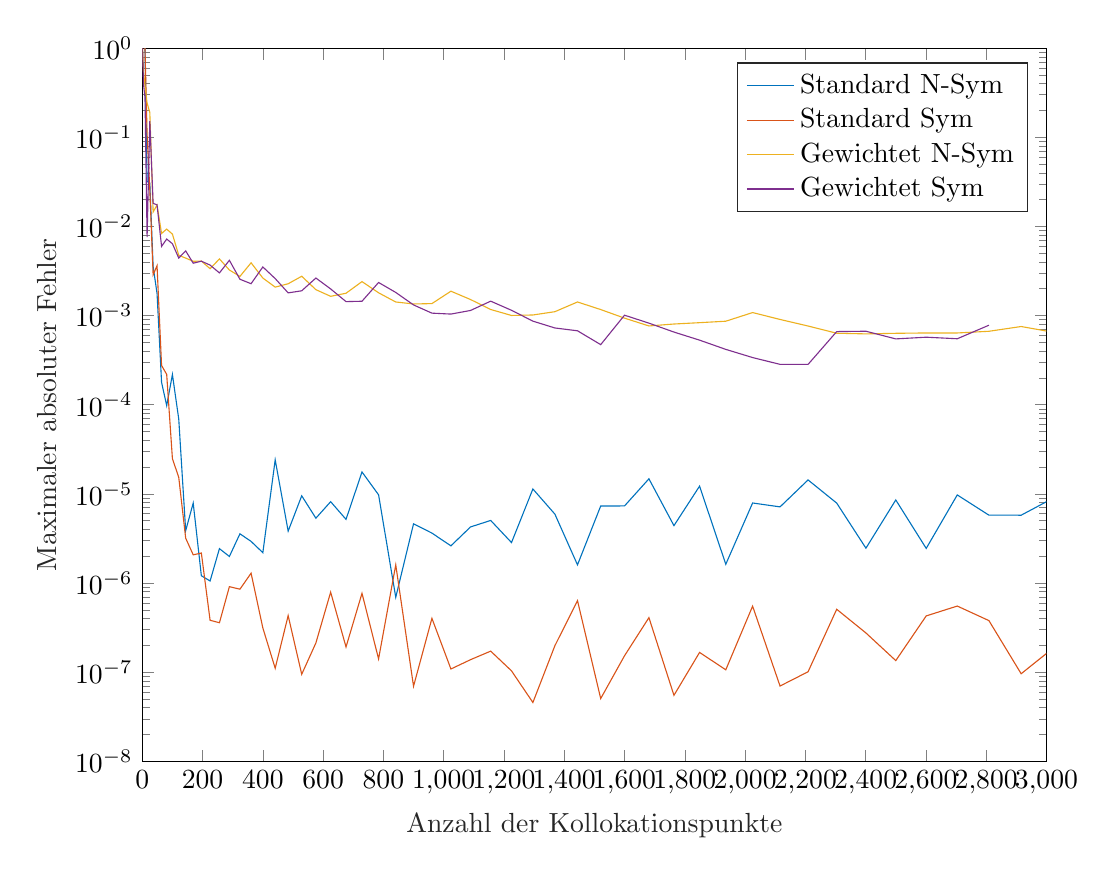
\begin{tikzpicture}

\begin{axis}[%
width=4.521in,
height=3.566in,
at={(0.758in,0.481in)},
scale only axis,
xmin=0,
xmax=3000,
xlabel style={font=\color{white!15!black}},
xlabel={Anzahl der Kollokationspunkte},
ymode=log,
ymin=1e-08,
ymax=1,
yminorticks=true,
ylabel style={font=\color{white!15!black}},
ylabel={Maximaler absoluter Fehler},
axis background/.style={fill=white},
%title style={font=\bfseries},
%title={error plot},
legend style={legend cell align=left, align=left, draw=white!15!black}
]
\addplot [color=mycolor1]
  table[row sep=crcr]{%
9	0.999748271191593\\
16	0.0320644506260388\\
25	0.0306339761398731\\
36	0.00355243728244914\\
49	0.0017737871617638\\
64	0.000178468537807508\\
81	9.79655766377152e-05\\
100	0.000218205946323484\\
121	6.93091783866319e-05\\
144	3.87155205178874e-06\\
169	7.89857892615972e-06\\
196	1.20896339392967e-06\\
225	1.05487836936369e-06\\
256	2.43333894801856e-06\\
289	1.98786725878752e-06\\
324	3.56903262012029e-06\\
361	2.93400357476159e-06\\
400	2.19234618849956e-06\\
441	2.41148464918128e-05\\
484	3.82455186892505e-06\\
529	9.52355613608596e-06\\
576	5.34194975650767e-06\\
625	8.18272606923492e-06\\
676	5.18289942128686e-06\\
729	1.76216574033043e-05\\
784	9.77439337927072e-06\\
841	6.92639750311808e-07\\
900	4.61993965032714e-06\\
961	3.63572091333086e-06\\
1024	2.61592994256141e-06\\
1089	4.26045828388899e-06\\
1156	5.0407949436504e-06\\
1225	2.84709437750087e-06\\
1296	1.13539168262317e-05\\
1369	5.9351437327812e-06\\
1444	1.60069958264966e-06\\
1521	7.32080172674565e-06\\
1600	7.33171671805227e-06\\
1681	1.47726674488147e-05\\
1764	4.40686918106586e-06\\
1849	1.22230332882944e-05\\
1936	1.62509643180514e-06\\
2025	7.91387876888233e-06\\
2116	7.15528588670147e-06\\
2209	1.43470301693371e-05\\
2304	7.89284950571123e-06\\
2401	2.46203996043075e-06\\
2500	8.55546425775067e-06\\
2601	2.44848604009917e-06\\
2704	9.7417097966318e-06\\
2809	5.77679670165504e-06\\
2916	5.77146360917352e-06\\
3025	9.06873058542298e-06\\
3136	2.22913705086869e-05\\
3249	1.08550523239409e-05\\
3364	4.80938577396284e-06\\
3481	6.94832855393374e-06\\
3600	1.12212729153349e-05\\
3721	4.09495018619671e-06\\
3844	2.38597305055391e-06\\
3969	4.47799881960267e-06\\
4096	1.89117200467478e-06\\
4225	3.08542426544905e-06\\
4356	4.48144153403912e-06\\
4489	4.76966269510881e-06\\
4624	8.71133417362779e-06\\
4761	6.55746477479235e-06\\
4900	7.21586046274758e-06\\
5041	4.90512203188843e-06\\
5184	7.98014494066135e-06\\
5329	2.46067336308721e-06\\
5476	4.09430751538431e-06\\
5625	5.44380397405134e-06\\
5776	1.4431355321351e-05\\
5929	8.68283233564429e-06\\
6084	9.07630273007734e-06\\
6241	4.01049026368429e-06\\
%6400	1.24298550654191e-05\\
};
\addlegendentry{Standard N-Sym}

\addplot [color=mycolor2]
  table[row sep=crcr]{%
9	0.999748271191593\\
16	0.107726668816776\\
25	0.0258124696186204\\
36	0.00287159725441316\\
49	0.00362599497445987\\
64	0.000275935163883759\\
81	0.00021918327793681\\
100	2.48216260381184e-05\\
121	1.53681446218856e-05\\
144	3.1884711230723e-06\\
169	2.07364346599404e-06\\
196	2.17226477314258e-06\\
225	3.82458048009404e-07\\
256	3.59086256618291e-07\\
289	9.11238147272009e-07\\
324	8.53447753842995e-07\\
361	1.29068967375662e-06\\
400	3.13765663895182e-07\\
441	1.10766025934739e-07\\
484	4.31307005194226e-07\\
529	9.47970708806145e-08\\
576	2.12821862091706e-07\\
625	7.90592467714291e-07\\
676	1.91874217403409e-07\\
729	7.67803314552506e-07\\
784	1.40958309802208e-07\\
841	1.60128464252868e-06\\
900	6.95889448287801e-08\\
961	4.01987755416222e-07\\
1024	1.08639425788759e-07\\
1089	1.38214763745204e-07\\
1156	1.72387506935934e-07\\
1225	1.03612470492287e-07\\
1296	4.576342060858e-08\\
1369	1.98436127196722e-07\\
1444	6.35113151403743e-07\\
1521	5.06464954974639e-08\\
1600	1.52946966314182e-07\\
1681	4.09538019885414e-07\\
1764	5.5073665183869e-08\\
1849	1.66687766992024e-07\\
1936	1.06468657223857e-07\\
2025	5.50868686666206e-07\\
2116 6.99989677332979e-08\\
2209	1.01204194941085e-07\\
2304	5.08060809312205e-07\\
2401	2.75578998398807e-07\\
2500	1.35024995649713e-07\\
2601	4.28100931787467e-07\\
2704	5.52255797536816e-07\\
2809	3.7940928332425e-07\\
2916	9.61568953350422e-08\\
3025	1.89729150917861e-07\\
3136	1.21232752281486e-07\\
3249	2.27521430473665e-07\\
3364	9.72793279263584e-08\\
3481	2.35286509470134e-07\\
3600 1.68344388165598e-07\\
3721	1.9990815880444e-07\\
3844 1.23043994684074e-07\\
3969 6.10004760037697e-08\\
4096	8.13971327007224e-08\\
4225	6.43811171041619e-08\\
4356	8.52963331077206e-08\\
4489	4.8430353877249e-07\\
4624	9.93239147595304e-08\\
4761	1.89865310695758e-07\\
4900	1.6717591381013e-07\\
5041	6.36370970363842e-08\\
5184	7.78480268026627e-08\\
5329	7.94766711331718e-08\\
5476	1.1111985875889e-07\\
5625	2.43472415561996e-08\\
5776	7.04574397714097e-08\\
5929	5.41579672358461e-08\\
6084	1.31851039864017e-07\\
6241	5.68597048888897e-08\\
%6400	8.04885743610484e-08\\
};
\addlegendentry{Standard Sym}

\addplot [color=mycolor3]
  table[row sep=crcr]{%
1	0.999748271191593\\
4	0.560545977774683\\
9	0.376431456467298\\
16	0.242193882415026\\
25	0.189993762183129\\
36	0.0145315966958548\\
49	0.0174041056649459\\
64	0.00834505059507007\\
81	0.00934238365437218\\
100	0.00820819260781327\\
121	0.00475244834379851\\
144	0.00441697660141732\\
169	0.00406748506379714\\
196	0.00409447866225437\\
225	0.0033579666972253\\
256	0.0043241172454006\\
289	0.00324914112411062\\
324	0.00275213023513118\\
361	0.00391365005302982\\
400	0.00263851914297952\\
441	0.00208792901895415\\
484	0.00227653749411576\\
529	0.00276465299973416\\
576	0.0019542410364516\\
625	0.00164619247351083\\
676	0.00178211660070896\\
729	0.00240678198216146\\
784	0.00180300901155017\\
841	0.00142159397516264\\
900	0.00135063363826503\\
961	0.00136403662517956\\
1024	0.00187889376605664\\
1089	0.00151567186145166\\
1156	0.00117112108272083\\
1225	0.00100375691133766\\
1296	0.00101656597379555\\
1369	0.00110672807043146\\
1444	0.00142218679845765\\
1521	0.00116947263868364\\
1600	0.000936762272438829\\
1681	0.000765759666293553\\
1764	0.000804976626695817\\
1849	0.000833372619874271\\
1936	0.000865284123169485\\
2025	0.00108191381491124\\
2116	0.000905641190680609\\
2209	0.000764516151901956\\
2304	0.000634176625289029\\
2401	0.000623958605345383\\
2500	0.00063335379648965\\
2601	0.000638937607292727\\
2704	0.000638760899761255\\
2809	0.000667173227936095\\
2916	0.000754851175303217\\
3025	0.000648325366486568\\
3136	0.000551523044055424\\
3249	0.000471442159094851\\
3364	0.000467246718358549\\
3481	0.00050288660343495\\
3600	0.000522592209090961\\
3721	0.00084098556409265\\
3844	0.000547093177643932\\
3969	0.000502654248024297\\
4096	0.000561280076275636\\
4225	0.000489822665259071\\
4356	0.000424579362970232\\
4489	0.00036908693801159\\
4624	0.00037973442375187\\
4761	0.000336686943717282\\
4900	0.000333247510963787\\
5041	0.000622394932566736\\
5184	0.000314427678619867\\
5329	0.000566880506456827\\
5476	0.000305234483597394\\
5625	0.000446349374714286\\
5776	0.000394865595689478\\
5929	0.000349251699575004\\
%6084	0.000309914170216655\\
};
\addlegendentry{Gewichtet N-Sym}

\addplot [color=mycolor4]
  table[row sep=crcr]{%
1	1\\
4	0.395035224833815\\
9	0.279941526477746\\
16	0.00757742098063802\\
25	0.15279986779413\\
36	0.0181867597368573\\
49	0.0174726143157827\\
64	0.0059766539555961\\
81	0.0072259913307462\\
100	0.00640403437702161\\
121	0.00442626411214436\\
144	0.00532310723804046\\
169	0.00387310797335394\\
196	0.00407996506526073\\
225	0.00368820159673228\\
256	0.00301329641393755\\
289	0.00417435519798021\\
324	0.00255717984883069\\
361	0.00228090820312338\\
400	0.00351398681638995\\
441	0.0026029916068597\\
484	0.00179911655500439\\
529	0.0018987095444248\\
576	0.00263945817673591\\
625	0.00199283880609186\\
676	0.00143566232698034\\
729	0.00144940556062869\\
784	0.0023538107588279\\
841	0.00181963638460381\\
900	0.00131781663419642\\
961	0.00106571464305072\\
1024	0.00104064262918289\\
1089	0.00114222240624102\\
1156	0.00145230809792884\\
1225	0.00114740561792823\\
1296	0.000866938209172496\\
1369	0.000726834193691045\\
1444	0.000675689848845577\\
1521	0.000472648830725779\\
1600	0.00101085556294689\\
1681	0.000823352891871659\\
1764	0.000653814864999019\\
1849	0.0005307186107327\\
1936	0.000418057941285993\\
2025	0.000338538094624863\\
2116	0.00028389945236007\\
2209	0.000283657173492734\\
2304	0.000662089880460209\\
2401	0.000668069445996095\\
2500	0.000548052209070699\\
2601	0.00057274203697291\\
2704	0.000550143031209322\\
2809	0.000780373496855821\\
};
\addlegendentry{Gewichtet Sym}

\end{axis}
\end{tikzpicture}%
%}
%\caption{Fehler der ersten \ac{PDE} bei Kollokationspunkten auf Gitter}
%\label{fig:error}
%\end{figure}
\begin{figure}[ht]
\centering
\resizebox {\columnwidth} {!} {
% This file was created by matlab2tikz.
%
%The latest updates can be retrieved from
%  http://www.mathworks.com/matlabcentral/fileexchange/22022-matlab2tikz-matlab2tikz
%where you can also make suggestions and rate matlab2tikz.
%
%
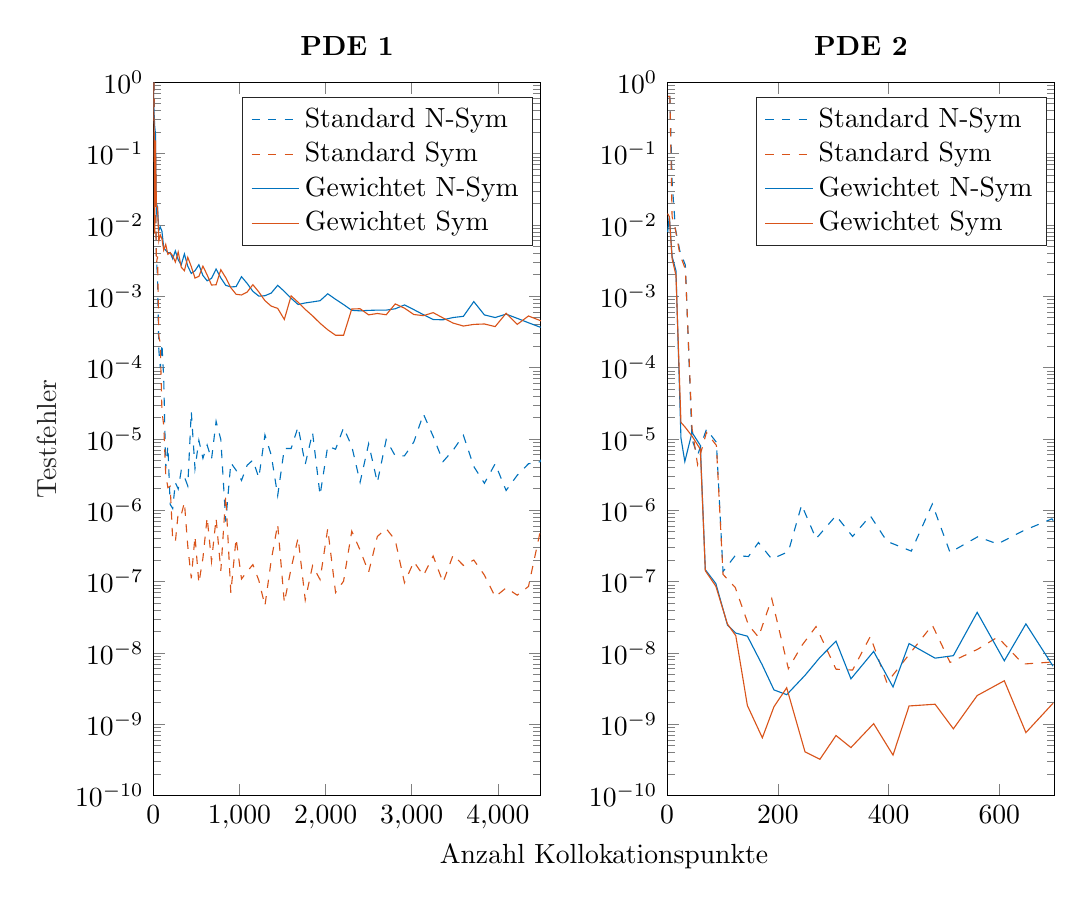
\begin{tikzpicture}

\begin{axis}[%
name = ax1,
width=1.938in,
height=3.566in,
at={(0.758in,0.481in)},
scale only axis,
xmin=0,
xmax=4500,
%xlabel style={font=\color{white!15!black}},
%xlabel={amount of collocation points},
ymode=log,
ymin=1e-10,
ymax=1,
yminorticks=true,
ylabel style={font=\color{white!15!black}},
ylabel={Testfehler},
axis background/.style={fill=white},
title style={font=\bfseries},
title={\ac{PDE} 1},
legend style={legend cell align=left, align=left, draw=white!15!black}
]
\addplot [color=mycolor1, dashed]
  table[row sep=crcr]{%
9	0.999748271191593\\
16	0.0320644506260388\\
25	0.0306339761398731\\
36	0.00355243728244914\\
49	0.0017737871617638\\
64	0.000178468537807508\\
81	9.79655766377152e-05\\
100	0.000218205946323484\\
121	6.93091783866319e-05\\
144	3.87155205178874e-06\\
169	7.89857892615972e-06\\
196	1.20896339392967e-06\\
225	1.05487836936369e-06\\
256	2.43333894801856e-06\\
289	1.98786725878752e-06\\
324	3.56903262012029e-06\\
361	2.93400357476159e-06\\
400	2.19234618849956e-06\\
441	2.41148464918128e-05\\
484	3.82455186892505e-06\\
529	9.52355613608596e-06\\
576	5.34194975650767e-06\\
625	8.18272606923492e-06\\
676	5.18289942128686e-06\\
729	1.76216574033043e-05\\
784	9.77439337927072e-06\\
841	6.92639750311808e-07\\
900	4.61993965032714e-06\\
961	3.63572091333086e-06\\
1024	2.61592994256141e-06\\
1089	4.26045828388899e-06\\
1156	5.0407949436504e-06\\
1225	2.84709437750087e-06\\
1296	1.13539168262317e-05\\
1369	5.9351437327812e-06\\
1444	1.60069958264966e-06\\
1521	7.32080172674565e-06\\
1600	7.33171671805227e-06\\
1681	1.47726674488147e-05\\
1764	4.40686918106586e-06\\
1849	1.22230332882944e-05\\
1936	1.62509643180514e-06\\
2025	7.91387876888233e-06\\
2116	7.15528588670147e-06\\
2209	1.43470301693371e-05\\
2304	7.89284950571123e-06\\
2401	2.46203996043075e-06\\
2500	8.55546425775067e-06\\
2601	2.44848604009917e-06\\
2704	9.7417097966318e-06\\
2809	5.77679670165504e-06\\
2916	5.77146360917352e-06\\
3025	9.06873058542298e-06\\
3136	2.22913705086869e-05\\
3249	1.08550523239409e-05\\
3364	4.80938577396284e-06\\
3481	6.94832855393374e-06\\
3600	1.12212729153349e-05\\
3721	4.09495018619671e-06\\
3844	2.38597305055391e-06\\
3969	4.47799881960267e-06\\
4096	1.89117200467478e-06\\
4225	3.08542426544905e-06\\
4356	4.48144153403912e-06\\
4489	4.76966269510881e-06\\
4624	8.71133417362779e-06\\
4761	6.55746477479235e-06\\
4900	7.21586046274758e-06\\
5041	4.90512203188843e-06\\
5184	7.98014494066135e-06\\
5329	2.46067336308721e-06\\
5476	4.09430751538431e-06\\
5625	5.44380397405134e-06\\
5776	1.4431355321351e-05\\
5929	8.68283233564429e-06\\
6084	9.07630273007734e-06\\
6241	4.01049026368429e-06\\
%6400	1.24298550654191e-05\\
};
\addlegendentry{Standard N-Sym}

\addplot [color=mycolor2, dashed]
  table[row sep=crcr]{%
9	0.999748271191593\\
16	0.107726668816776\\
25	0.0258124696186204\\
36	0.00287159725441316\\
49	0.00362599497445987\\
64	0.000275935163883759\\
81	0.00021918327793681\\
100	2.48216260381184e-05\\
121	1.53681446218856e-05\\
144	3.1884711230723e-06\\
169	2.07364346599404e-06\\
196	2.17226477314258e-06\\
225	3.82458048009404e-07\\
256	3.59086256618291e-07\\
289	9.11238147272009e-07\\
324	8.53447753842995e-07\\
361	1.29068967375662e-06\\
400	3.13765663895182e-07\\
441	1.10766025934739e-07\\
484	4.31307005194226e-07\\
529	9.47970708806145e-08\\
576	2.12821862091706e-07\\
625	7.90592467714291e-07\\
676	1.91874217403409e-07\\
729	7.67803314552506e-07\\
784	1.40958309802208e-07\\
841	1.60128464252868e-06\\
900	6.95889448287801e-08\\
961	4.01987755416222e-07\\
1024	1.08639425788759e-07\\
1089	1.38214763745204e-07\\
1156	1.72387506935934e-07\\
1225	1.03612470492287e-07\\
1296	4.576342060858e-08\\
1369	1.98436127196722e-07\\
1444	6.35113151403743e-07\\
1521	5.06464954974639e-08\\
1600	1.52946966314182e-07\\
1681	4.09538019885414e-07\\
1764	5.5073665183869e-08\\
1849	1.66687766992024e-07\\
1936	1.06468657223857e-07\\
2025	5.50868686666206e-07\\
2116 6.99989677332979e-08\\
2209	1.01204194941085e-07\\
2304	5.08060809312205e-07\\
2401	2.75578998398807e-07\\
2500	1.35024995649713e-07\\
2601	4.28100931787467e-07\\
2704	5.52255797536816e-07\\
2809	3.7940928332425e-07\\
2916	9.61568953350422e-08\\
3025	1.89729150917861e-07\\
3136	1.21232752281486e-07\\
3249	2.27521430473665e-07\\
3364	9.72793279263584e-08\\
3481	2.35286509470134e-07\\
3600 1.68344388165598e-07\\
3721	1.9990815880444e-07\\
3844 1.23043994684074e-07\\
3969 6.10004760037697e-08\\
4096	8.13971327007224e-08\\
4225	6.43811171041619e-08\\
4356	8.52963331077206e-08\\
4489	4.8430353877249e-07\\
4624	9.93239147595304e-08\\
4761	1.89865310695758e-07\\
4900	1.6717591381013e-07\\
5041	6.36370970363842e-08\\
5184	7.78480268026627e-08\\
5329	7.94766711331718e-08\\
5476	1.1111985875889e-07\\
5625	2.43472415561996e-08\\
5776	7.04574397714097e-08\\
5929	5.41579672358461e-08\\
6084	1.31851039864017e-07\\
6241	5.68597048888897e-08\\
%6400	8.04885743610484e-08\\
};
\addlegendentry{Standard Sym}

\addplot [color=mycolor1]
  table[row sep=crcr]{%
1	0.999748271191593\\
4	0.560545977774683\\
9	0.376431456467298\\
16	0.242193882415026\\
25	0.189993762183129\\
36	0.0145315966958548\\
49	0.0174041056649459\\
64	0.00834505059507007\\
81	0.00934238365437218\\
100	0.00820819260781327\\
121	0.00475244834379851\\
144	0.00441697660141732\\
169	0.00406748506379714\\
196	0.00409447866225437\\
225	0.0033579666972253\\
256	0.0043241172454006\\
289	0.00324914112411062\\
324	0.00275213023513118\\
361	0.00391365005302982\\
400	0.00263851914297952\\
441	0.00208792901895415\\
484	0.00227653749411576\\
529	0.00276465299973416\\
576	0.0019542410364516\\
625	0.00164619247351083\\
676	0.00178211660070896\\
729	0.00240678198216146\\
784	0.00180300901155017\\
841	0.00142159397516264\\
900	0.00135063363826503\\
961	0.00136403662517956\\
1024	0.00187889376605664\\
1089	0.00151567186145166\\
1156	0.00117112108272083\\
1225	0.00100375691133766\\
1296	0.00101656597379555\\
1369	0.00110672807043146\\
1444	0.00142218679845765\\
1521	0.00116947263868364\\
1600	0.000936762272438829\\
1681	0.000765759666293553\\
1764	0.000804976626695817\\
1849	0.000833372619874271\\
1936	0.000865284123169485\\
2025	0.00108191381491124\\
2116	0.000905641190680609\\
2209	0.000764516151901956\\
2304	0.000634176625289029\\
2401	0.000623958605345383\\
2500	0.00063335379648965\\
2601	0.000638937607292727\\
2704	0.000638760899761255\\
2809	0.000667173227936095\\
2916	0.000754851175303217\\
3025	0.000648325366486568\\
3136	0.000551523044055424\\
3249	0.000471442159094851\\
3364	0.000467246718358549\\
3481	0.00050288660343495\\
3600	0.000522592209090961\\
3721	0.00084098556409265\\
3844	0.000547093177643932\\
3969	0.000502654248024297\\
4096	0.000561280076275636\\
4225	0.000489822665259071\\
4356	0.000424579362970232\\
4489	0.00036908693801159\\
4624	0.00037973442375187\\
4761	0.000336686943717282\\
4900	0.000333247510963787\\
5041	0.000622394932566736\\
5184	0.000314427678619867\\
5329	0.000566880506456827\\
5476	0.000305234483597394\\
5625	0.000446349374714286\\
5776	0.000394865595689478\\
5929	0.000349251699575004\\
%6084	0.000309914170216655\\
};
\addlegendentry{Gewichtet N-Sym}

\addplot [color=mycolor2]
  table[row sep=crcr]{%
1	1\\
4	0.395035224833815\\
9	0.279941526477746\\
16	0.00757742098063802\\
25	0.15279986779413\\
36	0.0181867597368573\\
49	0.0174726143157827\\
64	0.0059766539555961\\
81	0.0072259913307462\\
100	0.00640403437702161\\
121	0.00442626411214436\\
144	0.00532310723804046\\
169	0.00387310797335394\\
196	0.00407996506526073\\
225	0.00368820159673228\\
256	0.00301329641393755\\
289	0.00417435519798021\\
324	0.00255717984883069\\
361	0.00228090820312338\\
400	0.00351398681638995\\
441	0.0026029916068597\\
484	0.00179911655500439\\
529	0.0018987095444248\\
576	0.00263945817673591\\
625	0.00199283880609186\\
676	0.00143566232698034\\
729	0.00144940556062869\\
784	0.0023538107588279\\
841	0.00181963638460381\\
900	0.00131781663419642\\
961	0.00106571464305072\\
1024	0.00104064262918289\\
1089	0.00114222240624102\\
1156	0.00145230809792884\\
1225	0.00114740561792823\\
1296	0.000866938209172496\\
1369	0.000726834193691045\\
1444	0.000675689848845577\\
1521	0.000472648830725779\\
1600	0.00101085556294689\\
1681	0.000823352891871659\\
1764	0.000653814864999019\\
1849	0.0005307186107327\\
1936	0.000418057941285993\\
2025	0.000338538094624863\\
2116	0.00028389945236007\\
2209	0.000283657173492734\\
2304	0.000662089880460209\\
2401	0.000668069445996095\\
2500	0.000548052209070699\\
2601	0.00057274203697291\\
2704	0.000550143031209322\\
2809	0.000780373496855821\\
2916	0.000679700162030026\\
3025	0.000554124481404688\\
3136	0.000534264270728673\\
3249	0.000588703082853276\\
3364	0.000496196208108826\\
3481	0.000420236042037947\\
3600	0.000381996696708446\\
3721	0.000402765973277075\\
3844	0.000408224335180239\\
3969	0.000375232616621\\
4096	0.00057646904252809\\
4225	0.000402872482652622\\
4356	0.00052837129152622\\
4489	0.000457389685535603\\
4624	0.000394568081179048\\
};
\addlegendentry{Gewichtet Sym}

\end{axis}

\begin{axis}[%
name = ax2,
width=1.938in,
height=3.566in,
at={(3.327in,0.481in)},
scale only axis,
xmin=0,
xmax=700,
%xlabel style={font=\color{white!15!black}},
%xlabel={amount of collocation points},
ymode=log,
ymin=1e-10,
ymax=1,
yminorticks=true,
%ylabel style={font=\color{white!15!black}},
%ylabel={max. error in derivative/absolute},
axis background/.style={fill=white},
title style={font=\bfseries},
title={\ac{PDE} 2},
legend style={legend cell align=left, align=left, draw=white!15!black}
]
\addplot [color=mycolor1, dashed]
  table[row sep=crcr]{%
2	0.631916518837427\\
5	0.631916518837427\\
9	0.0405336006196554\\
15	0.00883209685636366\\
23	0.00430857034180082\\
33	0.00272883525232875\\
45	9.77739763419194e-06\\
55	5.87763883978798e-06\\
71	1.36196952111728e-05\\
89	8.96739386711809e-06\\
101	1.37897394239528e-07\\
123	2.30675160362449e-07\\
147	2.24406043296266e-07\\
165	3.52200691985938e-07\\
189	2.06904876114133e-07\\
219	2.61886160706978e-07\\
243	1.1863207811675e-06\\
269	3.98191725909216e-07\\
305	8.37823561639084e-07\\
335	4.28710712069291e-07\\
367	8.35429125520737e-07\\
397	3.65824390795647e-07\\
441	2.67227388203728e-07\\
479	1.22109189190753e-06\\
511	2.55600133445763e-07\\
561	4.24029023692041e-07\\
597	3.35944663247545e-07\\
643	5.14170673207408e-07\\
695	7.56179082045394e-07\\
737	2.80417328014232e-07\\
789	7.42245731516489e-07\\
};
\addlegendentry{Standard N-Sym}

\addplot [color=mycolor2, dashed]
  table[row sep=crcr]{%
2	0.631916518837427\\
5	0.631916518837427\\
9	0.0131196754360414\\
15	0.00861983016720813\\
23	0.00388812001538674\\
33	0.00239333037518191\\
45	1.40699607112382e-05\\
55	4.35500602019578e-06\\
71	1.23129598888494e-05\\
89	8.10392788447301e-06\\
101	1.25844268880626e-07\\
123	8.2670365733617e-08\\
147	2.44909181754127e-08\\
165	1.66449326891027e-08\\
189	5.74401967604748e-08\\
219	5.99240512766386e-09\\
243	1.25718026371124e-08\\
269	2.33486955325546e-08\\
305	5.89867804948185e-09\\
335	5.73415277066447e-09\\
367	1.69623597390256e-08\\
397	3.80944553679541e-09\\
441	1.03664530293202e-08\\
479	2.44956352979386e-08\\
511	7.3530775634989e-09\\
561	1.12447527678139e-08\\
597	1.66316237448783e-08\\
643	6.96026979801756e-09\\
695	7.42834863065589e-09\\
737	2.59786652190286e-08\\
789	6.3033082087216e-09\\
};
\addlegendentry{Standard Sym}

\addplot [color=mycolor1]
  table[row sep=crcr]{%
1	0.00794443935648381\\
4	0.0133017612019765\\
9	0.00362254811444734\\
16	0.0022780437581805\\
25	1.03131710251503e-05\\
32	4.81181204470271e-06\\
45	1.23029704517386e-05\\
60	8.09775474910901e-06\\
69	1.46364200204196e-07\\
88	9.37122425770376e-08\\
109	2.45793275871486e-08\\
124	1.89336762171366e-08\\
145	1.71188485817431e-08\\
172	6.72586053518387e-09\\
193	3.01951863512784e-09\\
216	2.59167542981942e-09\\
249	4.8303522293125e-09\\
276	8.62708293691838e-09\\
305	1.46005317835929e-08\\
332	4.32146185502802e-09\\
373	1.04669000133839e-08\\
408	3.32050553719654e-09\\
437	1.34985452815428e-08\\
484	8.42141356649506e-09\\
517	9.12785619311407e-09\\
560	3.69603436745081e-08\\
609	7.73561570355241e-09\\
648	2.54551856260221e-08\\
697	6.51625686742818e-09\\
};
\addlegendentry{Gewichtet N-Sym}

\addplot [color=mycolor2]
  table[row sep=crcr]{%
1	0.0143846214789116\\
4	0.0130604160741108\\
9	0.00336559573493192\\
16	0.00196288047392809\\
25	1.70127111368545e-05\\
32	1.47805455507494e-05\\
45	1.09439169746484e-05\\
60	7.15540904007439e-06\\
69	1.41731398284328e-07\\
88	8.6057435927378e-08\\
109	2.52869050906823e-08\\
124	1.74264397634349e-08\\
145	1.82477661453406e-09\\
172	6.43924830123765e-10\\
193	1.75784165001858e-09\\
216	3.23772897381502e-09\\
249	4.0984393656629e-10\\
276	3.21971893590955e-10\\
305	6.92943258329137e-10\\
332	4.69699390492906e-10\\
373	1.01659414220023e-09\\
408	3.68062358369059e-10\\
437	1.79956516355162e-09\\
484	1.90341531425275e-09\\
517	8.60199689256547e-10\\
560	2.51715981391953e-09\\
609	4.06107103501085e-09\\
648	7.61975038621188e-10\\
697	1.96490679282846e-09\\
};
\addlegendentry{Gewichtet Sym}

\end{axis}
\path (ax1.south east) -- (ax2.south west)
  node[midway,below=5mm] {Anzahl Kollokationspunkte};
\end{tikzpicture}%
}
\caption{Testfehler bei Kollokationspunkten auf einem Gitter}
\label{fig:error-grid-both}
\end{figure}

Wir stellen als erstes fest, dass alle Verfahren vernünftige Ergebnisse liefern und gegen die analytische Lösung konvergieren. Unsere theoretische Herleitung war demnach also sinnvoll. Wir sehen aber deutliche Unterschiede zwischen den beiden \acp{PDE}.

Für die erste \ac{PDE} liefern die Standardverfahren bereits mit nahezu $200$ Kollokationspunkten ihre besten Ergebnisse mit einem Testfehler in der Größenordnung von $10^{-6}$ für das nicht-symmetrische Verfahren und $10^{-7}$ für das symmetrische und verbessern sich danach nicht mehr. Im Gegensatz dazu stehen die gewichteten Verfahren, die am Anfang bei weitem nicht so gute Ergebnisse von rund einem Testfehler von $10^{-2}$ liefern, sich dann aber mit mehr Kollokationspunkten noch leicht verbessern. Gesamt erreichen die gewichteten Verfahren aber selbst mit $4500$ Kollokationspunkten nicht die Genauigkeit der Standardverfahren. Im Vergleich der symmetrischen und nicht-symmetrischen Verfahren schneidet beim Standardverfahren das symmetrische leicht besser ab, beim gewichteten ist kein Unterschied erkennbar.

Ein Grund für das schlechtere Abschneiden der gewichteten Verfahren wird erkennbar, wenn man sich anschaut, wo der große Fehler angenommen wird. Der Testfehler des gewichteten nicht-symmetrischen Verfahrens mit $529$ Kollokationspunkten auf dem Gebiet $\Omega$ ist in Abbildung \ref{fig:Vergleich} dargestellt.

\begin{figure}[ht]
\centering
\resizebox {.7\columnwidth} {!} {
% This file was created by matlab2tikz.
%
%The latest updates can be retrieved from
%  http://www.mathworks.com/matlabcentral/fileexchange/22022-matlab2tikz-matlab2tikz
%where you can also make suggestions and rate matlab2tikz.
%
\begin{tikzpicture}

\begin{axis}[%
width=3.972in,
height=3.566in,
at={(0.666in,0.481in)},
scale only axis,
point meta min=0,
point meta max=0.00278001741363055,
xmin=-1,
xmax=1,
ymin=-1,
ymax=1,
axis background/.style={fill=white},
title style={font=\bfseries},
title={absolute error when compared to exact solution},
legend style={legend cell align=left, align=left, draw=white!15!black},
colormap={mymap}{[1pt] rgb(0pt)=(0.2422,0.1504,0.6603); rgb(1pt)=(0.25039,0.164995,0.707614); rgb(2pt)=(0.257771,0.181781,0.751138); rgb(3pt)=(0.264729,0.197757,0.795214); rgb(4pt)=(0.270648,0.214676,0.836371); rgb(5pt)=(0.275114,0.234238,0.870986); rgb(6pt)=(0.2783,0.255871,0.899071); rgb(7pt)=(0.280333,0.278233,0.9221); rgb(8pt)=(0.281338,0.300595,0.941376); rgb(9pt)=(0.281014,0.322757,0.957886); rgb(10pt)=(0.279467,0.344671,0.971676); rgb(11pt)=(0.275971,0.366681,0.982905); rgb(12pt)=(0.269914,0.3892,0.9906); rgb(13pt)=(0.260243,0.412329,0.995157); rgb(14pt)=(0.244033,0.435833,0.998833); rgb(15pt)=(0.220643,0.460257,0.997286); rgb(16pt)=(0.196333,0.484719,0.989152); rgb(17pt)=(0.183405,0.507371,0.979795); rgb(18pt)=(0.178643,0.528857,0.968157); rgb(19pt)=(0.176438,0.549905,0.952019); rgb(20pt)=(0.168743,0.570262,0.935871); rgb(21pt)=(0.154,0.5902,0.9218); rgb(22pt)=(0.146029,0.609119,0.907857); rgb(23pt)=(0.138024,0.627629,0.89729); rgb(24pt)=(0.124814,0.645929,0.888343); rgb(25pt)=(0.111252,0.6635,0.876314); rgb(26pt)=(0.0952095,0.679829,0.859781); rgb(27pt)=(0.0688714,0.694771,0.839357); rgb(28pt)=(0.0296667,0.708167,0.816333); rgb(29pt)=(0.00357143,0.720267,0.7917); rgb(30pt)=(0.00665714,0.731214,0.766014); rgb(31pt)=(0.0433286,0.741095,0.73941); rgb(32pt)=(0.0963952,0.75,0.712038); rgb(33pt)=(0.140771,0.7584,0.684157); rgb(34pt)=(0.1717,0.766962,0.655443); rgb(35pt)=(0.193767,0.775767,0.6251); rgb(36pt)=(0.216086,0.7843,0.5923); rgb(37pt)=(0.246957,0.791795,0.556743); rgb(38pt)=(0.290614,0.79729,0.518829); rgb(39pt)=(0.340643,0.8008,0.478857); rgb(40pt)=(0.3909,0.802871,0.435448); rgb(41pt)=(0.445629,0.802419,0.390919); rgb(42pt)=(0.5044,0.7993,0.348); rgb(43pt)=(0.561562,0.794233,0.304481); rgb(44pt)=(0.617395,0.787619,0.261238); rgb(45pt)=(0.671986,0.779271,0.2227); rgb(46pt)=(0.7242,0.769843,0.191029); rgb(47pt)=(0.773833,0.759805,0.16461); rgb(48pt)=(0.820314,0.749814,0.153529); rgb(49pt)=(0.863433,0.7406,0.159633); rgb(50pt)=(0.903543,0.733029,0.177414); rgb(51pt)=(0.939257,0.728786,0.209957); rgb(52pt)=(0.972757,0.729771,0.239443); rgb(53pt)=(0.995648,0.743371,0.237148); rgb(54pt)=(0.996986,0.765857,0.219943); rgb(55pt)=(0.995205,0.789252,0.202762); rgb(56pt)=(0.9892,0.813567,0.188533); rgb(57pt)=(0.978629,0.838629,0.176557); rgb(58pt)=(0.967648,0.8639,0.16429); rgb(59pt)=(0.96101,0.889019,0.153676); rgb(60pt)=(0.959671,0.913457,0.142257); rgb(61pt)=(0.962795,0.937338,0.12651); rgb(62pt)=(0.969114,0.960629,0.106362); rgb(63pt)=(0.9769,0.9839,0.0805)},
colorbar
]

\addplot[%
surf,
shader=flat corner, draw=black, colormap={mymap}{[1pt] rgb(0pt)=(0.2422,0.1504,0.6603); rgb(1pt)=(0.25039,0.164995,0.707614); rgb(2pt)=(0.257771,0.181781,0.751138); rgb(3pt)=(0.264729,0.197757,0.795214); rgb(4pt)=(0.270648,0.214676,0.836371); rgb(5pt)=(0.275114,0.234238,0.870986); rgb(6pt)=(0.2783,0.255871,0.899071); rgb(7pt)=(0.280333,0.278233,0.9221); rgb(8pt)=(0.281338,0.300595,0.941376); rgb(9pt)=(0.281014,0.322757,0.957886); rgb(10pt)=(0.279467,0.344671,0.971676); rgb(11pt)=(0.275971,0.366681,0.982905); rgb(12pt)=(0.269914,0.3892,0.9906); rgb(13pt)=(0.260243,0.412329,0.995157); rgb(14pt)=(0.244033,0.435833,0.998833); rgb(15pt)=(0.220643,0.460257,0.997286); rgb(16pt)=(0.196333,0.484719,0.989152); rgb(17pt)=(0.183405,0.507371,0.979795); rgb(18pt)=(0.178643,0.528857,0.968157); rgb(19pt)=(0.176438,0.549905,0.952019); rgb(20pt)=(0.168743,0.570262,0.935871); rgb(21pt)=(0.154,0.5902,0.9218); rgb(22pt)=(0.146029,0.609119,0.907857); rgb(23pt)=(0.138024,0.627629,0.89729); rgb(24pt)=(0.124814,0.645929,0.888343); rgb(25pt)=(0.111252,0.6635,0.876314); rgb(26pt)=(0.0952095,0.679829,0.859781); rgb(27pt)=(0.0688714,0.694771,0.839357); rgb(28pt)=(0.0296667,0.708167,0.816333); rgb(29pt)=(0.00357143,0.720267,0.7917); rgb(30pt)=(0.00665714,0.731214,0.766014); rgb(31pt)=(0.0433286,0.741095,0.73941); rgb(32pt)=(0.0963952,0.75,0.712038); rgb(33pt)=(0.140771,0.7584,0.684157); rgb(34pt)=(0.1717,0.766962,0.655443); rgb(35pt)=(0.193767,0.775767,0.6251); rgb(36pt)=(0.216086,0.7843,0.5923); rgb(37pt)=(0.246957,0.791795,0.556743); rgb(38pt)=(0.290614,0.79729,0.518829); rgb(39pt)=(0.340643,0.8008,0.478857); rgb(40pt)=(0.3909,0.802871,0.435448); rgb(41pt)=(0.445629,0.802419,0.390919); rgb(42pt)=(0.5044,0.7993,0.348); rgb(43pt)=(0.561562,0.794233,0.304481); rgb(44pt)=(0.617395,0.787619,0.261238); rgb(45pt)=(0.671986,0.779271,0.2227); rgb(46pt)=(0.7242,0.769843,0.191029); rgb(47pt)=(0.773833,0.759805,0.16461); rgb(48pt)=(0.820314,0.749814,0.153529); rgb(49pt)=(0.863433,0.7406,0.159633); rgb(50pt)=(0.903543,0.733029,0.177414); rgb(51pt)=(0.939257,0.728786,0.209957); rgb(52pt)=(0.972757,0.729771,0.239443); rgb(53pt)=(0.995648,0.743371,0.237148); rgb(54pt)=(0.996986,0.765857,0.219943); rgb(55pt)=(0.995205,0.789252,0.202762); rgb(56pt)=(0.9892,0.813567,0.188533); rgb(57pt)=(0.978629,0.838629,0.176557); rgb(58pt)=(0.967648,0.8639,0.16429); rgb(59pt)=(0.96101,0.889019,0.153676); rgb(60pt)=(0.959671,0.913457,0.142257); rgb(61pt)=(0.962795,0.937338,0.12651); rgb(62pt)=(0.969114,0.960629,0.106362); rgb(63pt)=(0.9769,0.9839,0.0805)}, mesh/rows=100]
table[row sep=crcr, point meta=\thisrow{c}] {%
%
x	y	c\\
-1	-1	1.49975978266186e-32\\
-0.97979797979798	-1	1.10171022151052e-16\\
-0.95959595959596	-1	5.97091774464293e-17\\
-0.939393939393939	-1	0\\
-0.919191919191919	-1	1.16258150442686e-16\\
-0.898989898989899	-1	0\\
-0.878787878787879	-1	4.55155236687665e-17\\
-0.858585858585859	-1	5.26346963379822e-17\\
-0.838383838383838	-1	0\\
-0.818181818181818	-1	6.62094046585406e-17\\
-0.797979797979798	-1	7.26102797505851e-17\\
-0.777777777777778	-1	1.46085237259516e-16\\
-0.757575757575758	-1	8.45103052570338e-17\\
-0.737373737373737	-1	8.99615384687633e-17\\
-0.717171717171717	-1	9.50505283164436e-17\\
-0.696969696969697	-1	9.97567832340851e-17\\
-0.676767676767677	-1	1.04061352794178e-16\\
-0.656565656565657	-1	1.07946904014375e-16\\
-0.636363636363636	-1	2.06155202468483e-16\\
-0.616161616161616	-1	1.14400118700401e-16\\
-0.595959595959596	-1	1.16941797348312e-16\\
-0.575757575757576	-1	1.19012592652179e-16\\
-0.555555555555556	-1	1.2060416625019e-16\\
-0.535353535353535	-1	1.217101094372e-16\\
-0.515151515151515	-1	1.2232596897033e-16\\
-0.494949494949495	-1	1.22449265000606e-16\\
-0.474747474747475	-1	1.2207950105843e-16\\
-0.454545454545455	-1	1.2121816605269e-16\\
-0.434343434343434	-1	1.19868728275453e-16\\
-0.414141414141414	-1	1.18036621436371e-16\\
-0.393939393939394	-1	2.12228094244675e-16\\
-0.373737373737374	-1	1.12955823395499e-16\\
-0.353535353535353	-1	1.09727590774184e-16\\
-0.333333333333333	-1	1.06057523872491e-16\\
-0.313131313131313	-1	1.01960400754505e-16\\
-0.292929292929293	-1	9.7452719088969e-17\\
-0.272727272727273	-1	9.25526297189917e-17\\
-0.252525252525252	-1	8.727986357501e-17\\
-0.232323232323232	-1	8.16556522252957e-17\\
-0.212121212121212	-1	7.57026423839237e-17\\
-0.191919191919192	-1	6.94448047204476e-17\\
-0.171717171717172	-1	6.29073373384734e-17\\
-0.151515151515151	-1	5.61165643117898e-17\\
-0.131313131313131	-1	4.90998296866144e-17\\
-0.111111111111111	-1	4.18853873767699e-17\\
-0.0909090909090909	-1	3.45022873951457e-17\\
-0.0707070707070707	-1	2.69802588795485e-17\\
-0.0505050505050505	-1	1.93495903839576e-17\\
-0.0303030303030303	-1	1.16410079172079e-17\\
-0.0101010101010101	-1	3.88555122019685e-18\\
0.0101010101010102	-1	3.88555122019689e-18\\
0.0303030303030303	-1	1.16410079172079e-17\\
0.0505050505050506	-1	1.93495903839577e-17\\
0.0707070707070707	-1	2.69802588795485e-17\\
0.0909090909090908	-1	3.45022873951456e-17\\
0.111111111111111	-1	4.18853873767699e-17\\
0.131313131313131	-1	4.90998296866144e-17\\
0.151515151515152	-1	5.61165643117898e-17\\
0.171717171717172	-1	6.29073373384734e-17\\
0.191919191919192	-1	6.94448047204476e-17\\
0.212121212121212	-1	7.57026423839237e-17\\
0.232323232323232	-1	8.16556522252956e-17\\
0.252525252525253	-1	8.727986357501e-17\\
0.272727272727273	-1	9.25526297189917e-17\\
0.292929292929293	-1	9.7452719088969e-17\\
0.313131313131313	-1	1.01960400754505e-16\\
0.333333333333333	-1	1.06057523872491e-16\\
0.353535353535354	-1	1.09727590774184e-16\\
0.373737373737374	-1	1.12955823395499e-16\\
0.393939393939394	-1	1.15729222783055e-16\\
0.414141414141414	-1	1.18036621436371e-16\\
0.434343434343434	-1	1.19868728275453e-16\\
0.454545454545455	-1	1.2121816605269e-16\\
0.474747474747475	-1	1.2207950105843e-16\\
0.494949494949495	-1	1.22449265000606e-16\\
0.515151515151515	-1	1.2232596897033e-16\\
0.535353535353535	-1	1.217101094372e-16\\
0.555555555555556	-1	1.2060416625019e-16\\
0.575757575757576	-1	1.19012592652179e-16\\
0.595959595959596	-1	1.16941797348312e-16\\
0.616161616161616	-1	1.14400118700401e-16\\
0.636363636363636	-1	1.11397791151293e-16\\
0.656565656565657	-1	1.07946904014375e-16\\
0.676767676767677	-1	1.04061352794178e-16\\
0.696969696969697	-1	9.97567832340851e-17\\
0.717171717171717	-1	9.50505283164436e-17\\
0.737373737373737	-1	8.99615384687633e-17\\
0.757575757575758	-1	8.45103052570338e-17\\
0.777777777777778	-1	7.87187788734199e-17\\
0.797979797979798	-1	7.26102797505851e-17\\
0.818181818181818	-1	6.62094046585406e-17\\
0.838383838383838	-1	1.07869154916183e-16\\
0.858585858585859	-1	5.26346963379822e-17\\
0.878787878787879	-1	4.55155236687665e-17\\
0.898989898989899	-1	0\\
0.919191919191919	-1	0\\
0.939393939393939	-1	0\\
0.95959595959596	-1	5.4675264181714e-17\\
0.97979797979798	-1	1.02197100108774e-16\\
1	-1	1.49975978266186e-32\\
-1	-0.97979797979798	0\\
-0.97979797979798	-0.97979797979798	0.00247416837228592\\
-0.95959595959596	-0.97979797979798	0.00242847188444572\\
-0.939393939393939	-0.97979797979798	0.00202035949499204\\
-0.919191919191919	-0.97979797979798	0.00157323396173768\\
-0.898989898989899	-0.97979797979798	0.00116512432854791\\
-0.878787878787879	-0.97979797979798	0.00081981169154817\\
-0.858585858585859	-0.97979797979798	0.000542009092715522\\
-0.838383838383838	-0.97979797979798	0.000327881023408125\\
-0.818181818181818	-0.97979797979798	0.000169640160496073\\
-0.797979797979798	-0.97979797979798	5.80762807525087e-05\\
-0.777777777777778	-0.97979797979798	1.5949815176948e-05\\
-0.757575757575758	-0.97979797979798	6.06763700097823e-05\\
-0.737373737373737	-0.97979797979798	8.30747630525194e-05\\
-0.717171717171717	-0.97979797979798	8.88001374503081e-05\\
-0.696969696969697	-0.97979797979798	8.23256371082701e-05\\
-0.676767676767677	-0.97979797979798	6.71563762008193e-05\\
-0.656565656565657	-0.97979797979798	4.6051362052775e-05\\
-0.636363636363636	-0.97979797979798	2.12092091448068e-05\\
-0.616161616161616	-0.97979797979798	5.60402152039591e-06\\
-0.595959595959596	-0.97979797979798	3.29701061415472e-05\\
-0.575757575757576	-0.97979797979798	5.97705268965756e-05\\
-0.555555555555556	-0.97979797979798	8.51502253902889e-05\\
-0.535353535353535	-0.97979797979798	0.000108484766196612\\
-0.515151515151515	-0.97979797979798	0.000129345399851474\\
-0.494949494949495	-0.97979797979798	0.000147461053628589\\
-0.474747474747475	-0.97979797979798	0.000162679913928709\\
-0.454545454545455	-0.97979797979798	0.000174946015650393\\
-0.434343434343434	-0.97979797979798	0.000184275054869572\\
-0.414141414141414	-0.97979797979798	0.000190752520179575\\
-0.393939393939394	-0.97979797979798	0.000194522734583306\\
-0.373737373737374	-0.97979797979798	0.000195781327760623\\
-0.353535353535353	-0.97979797979798	0.000194772937355245\\
-0.333333333333333	-0.97979797979798	0.000191763013221082\\
-0.313131313131313	-0.97979797979798	0.000187010985244852\\
-0.292929292929293	-0.97979797979798	0.000180753127756249\\
-0.272727272727273	-0.97979797979798	0.000173176711585434\\
-0.252525252525252	-0.97979797979798	0.000164413411597418\\
-0.232323232323232	-0.97979797979798	0.000154549357597768\\
-0.212121212121212	-0.97979797979798	0.000143635682565216\\
-0.191919191919192	-0.97979797979798	0.000131716915056097\\
-0.171717171717172	-0.97979797979798	0.000118851005121781\\
-0.151515151515151	-0.97979797979798	0.000105135136114085\\
-0.131313131313131	-0.97979797979798	9.0689688046184e-05\\
-0.111111111111111	-0.97979797979798	7.56743357918296e-05\\
-0.0909090909090909	-0.97979797979798	6.0254062069446e-05\\
-0.0707070707070707	-0.97979797979798	4.45842424167172e-05\\
-0.0505050505050505	-0.97979797979798	2.87797234341039e-05\\
-0.0303030303030303	-0.97979797979798	1.29133594552371e-05\\
-0.0101010101010101	-0.97979797979798	2.98097365935028e-06\\
0.0101010101010102	-0.97979797979798	1.89052389634502e-05\\
0.0303030303030303	-0.97979797979798	3.48776322529037e-05\\
0.0505050505050506	-0.97979797979798	5.08928060032401e-05\\
0.0707070707070707	-0.97979797979798	6.69212539360399e-05\\
0.0909090909090908	-0.97979797979798	8.28863994997847e-05\\
0.111111111111111	-0.97979797979798	9.86583605299546e-05\\
0.131313131313131	-0.97979797979798	0.000114084822278128\\
0.151515151515152	-0.97979797979798	0.000128994369680276\\
0.171717171717172	-0.97979797979798	0.000143222296778829\\
0.191919191919192	-0.97979797979798	0.000156622350492922\\
0.212121212121212	-0.97979797979798	0.000169080516589128\\
0.232323232323232	-0.97979797979798	0.000180499383258884\\
0.252525252525253	-0.97979797979798	0.000190783532332116\\
0.272727272727273	-0.97979797979798	0.000199816438347593\\
0.292929292929293	-0.97979797979798	0.000207435710958354\\
0.313131313131313	-0.97979797979798	0.000213418937015701\\
0.333333333333333	-0.97979797979798	0.000217469843803358\\
0.353535353535354	-0.97979797979798	0.000219251485938037\\
0.373737373737374	-0.97979797979798	0.000218397070570329\\
0.393939393939394	-0.97979797979798	0.000214557885639247\\
0.414141414141414	-0.97979797979798	0.000207430272164126\\
0.434343434343434	-0.97979797979798	0.000196790366766342\\
0.454545454545455	-0.97979797979798	0.00018251123033626\\
0.474747474747475	-0.97979797979798	0.000164573650197147\\
0.494949494949495	-0.97979797979798	0.000143063018727657\\
0.515151515151515	-0.97979797979798	0.000118164231979204\\
0.535353535353535	-0.97979797979798	9.01871834552009e-05\\
0.555555555555556	-0.97979797979798	5.95682030752887e-05\\
0.575757575757576	-0.97979797979798	2.69175849295089e-05\\
0.595959595959596	-0.97979797979798	6.94306618501811e-06\\
0.616161616161616	-0.97979797979798	4.09219673098843e-05\\
0.636363636363636	-0.97979797979798	7.36288992513948e-05\\
0.656565656565657	-0.97979797979798	0.000103323208032739\\
0.676767676767677	-0.97979797979798	0.000127881815483268\\
0.696969696969697	-0.97979797979798	0.00014473369738717\\
0.717171717171717	-0.97979797979798	0.000150785149742434\\
0.737373737373737	-0.97979797979798	0.000142272332851995\\
0.757575757575758	-0.97979797979798	0.000114586407336373\\
0.777777777777778	-0.97979797979798	6.20926505393166e-05\\
0.797979797979798	-0.97979797979798	2.20061559784782e-05\\
0.818181818181818	-0.97979797979798	0.000145636297035866\\
0.838383838383838	-0.97979797979798	0.000317511695477064\\
0.858585858585859	-0.97979797979798	0.000546317476269823\\
0.878787878787879	-0.97979797979798	0.000839177732394877\\
0.898989898989899	-0.97979797979798	0.00119901010510942\\
0.919191919191919	-0.97979797979798	0.00161970121346812\\
0.939393939393939	-0.97979797979798	0.00207520654402618\\
0.95959595959596	-0.97979797979798	0.0024837069106058\\
0.97979797979798	-0.97979797979798	0.00251486362462505\\
1	-0.97979797979798	0\\
-1	-0.95959595959596	3.31176937676246e-17\\
-0.97979797979798	-0.95959595959596	0.00257419906433284\\
-0.95959595959596	-0.95959595959596	0.00278001741363055\\
-0.939393939393939	-0.95959595959596	0.002422745274826\\
-0.919191919191919	-0.95959595959596	0.00196121064914878\\
-0.898989898989899	-0.95959595959596	0.001515198713464\\
-0.878787878787879	-0.95959595959596	0.00112192376658306\\
-0.858585858585859	-0.95959595959596	0.000792956838088194\\
-0.838383838383838	-0.95959595959596	0.00052910126880816\\
-0.818181818181818	-0.95959595959596	0.000325722349252211\\
-0.797979797979798	-0.95959595959596	0.000175452997565384\\
-0.777777777777778	-0.95959595959596	6.99058253335327e-05\\
-0.757575757575758	-0.95959595959596	7.71282621034319e-07\\
-0.737373737373737	-0.95959595959596	3.95271397071878e-05\\
-0.717171717171717	-0.95959595959596	5.75298634414995e-05\\
-0.696969696969697	-0.95959595959596	5.86909161623822e-05\\
-0.676767676767677	-0.95959595959596	4.7463783006782e-05\\
-0.656565656565657	-0.95959595959596	2.74582433327369e-05\\
-0.636363636363636	-0.95959595959596	1.59941621609427e-06\\
-0.616161616161616	-0.95959595959596	2.77401805308247e-05\\
-0.595959595959596	-0.95959595959596	5.86467870252738e-05\\
-0.575757575757576	-0.95959595959596	8.95939676661961e-05\\
-0.555555555555556	-0.95959595959596	0.000119393794570197\\
-0.535353535353535	-0.95959595959596	0.000147159987692769\\
-0.515151515151515	-0.95959595959596	0.000172252880564688\\
-0.494949494949495	-0.95959595959596	0.000194241382177496\\
-0.474747474747475	-0.95959595959596	0.000212858214358375\\
-0.454545454545455	-0.95959595959596	0.000227966548890624\\
-0.434343434343434	-0.95959595959596	0.000239535796304022\\
-0.414141414141414	-0.95959595959596	0.000247630355437761\\
-0.393939393939394	-0.95959595959596	0.000252389394020308\\
-0.373737373737374	-0.95959595959596	0.000254028270312304\\
-0.353535353535353	-0.95959595959596	0.000252814961272524\\
-0.333333333333333	-0.95959595959596	0.000249047787666615\\
-0.313131313131313	-0.95959595959596	0.000243026725788617\\
-0.292929292929293	-0.95959595959596	0.000235029842662562\\
-0.272727272727273	-0.95959595959596	0.000225280512459056\\
-0.252525252525252	-0.95959595959596	0.000213950755449263\\
-0.232323232323232	-0.95959595959596	0.000201157383345654\\
-0.212121212121212	-0.95959595959596	0.000186981717326243\\
-0.191919191919192	-0.95959595959596	0.000171497230494658\\
-0.171717171717172	-0.95959595959596	0.000154792556343139\\
-0.151515151515151	-0.95959595959596	0.000136992161857072\\
-0.131313131313131	-0.95959595959596	0.000118252654054816\\
-0.111111111111111	-0.95959595959596	9.87652096269484e-05\\
-0.0909090909090909	-0.95959595959596	7.8732665909971e-05\\
-0.0707070707070707	-0.95959595959596	5.83321975287827e-05\\
-0.0505050505050505	-0.95959595959596	3.77205972353599e-05\\
-0.0303030303030303	-0.95959595959596	1.6988829864735e-05\\
-0.0101010101010101	-0.95959595959596	3.80310253678996e-06\\
0.0101010101010102	-0.95959595959596	2.46427225197065e-05\\
0.0303030303030303	-0.95959595959596	4.55252771338933e-05\\
0.0505050505050506	-0.95959595959596	6.64248103895287e-05\\
0.0707070707070707	-0.95959595959596	8.72860784163834e-05\\
0.0909090909090908	-0.95959595959596	0.000108002001387643\\
0.111111111111111	-0.95959595959596	0.000128422978804284\\
0.131313131313131	-0.95959595959596	0.000148352910711476\\
0.151515151515152	-0.95959595959596	0.000167582674213004\\
0.171717171717172	-0.95959595959596	0.000185909419170099\\
0.191919191919192	-0.95959595959596	0.000203146737857818\\
0.212121212121212	-0.95959595959596	0.000219137932397487\\
0.232323232323232	-0.95959595959596	0.00023374434166\\
0.252525252525253	-0.95959595959596	0.000246831553585208\\
0.272727272727273	-0.95959595959596	0.000258226761101821\\
0.292929292929293	-0.95959595959596	0.000267723222040994\\
0.313131313131313	-0.95959595959596	0.000275038677669801\\
0.333333333333333	-0.95959595959596	0.000279820192898822\\
0.353535353535354	-0.95959595959596	0.000281674305092114\\
0.373737373737374	-0.95959595959596	0.000280178780426368\\
0.393939393939394	-0.95959595959596	0.000274934222785128\\
0.414141414141414	-0.95959595959596	0.000265604172035139\\
0.434343434343434	-0.95959595959596	0.000251952642561698\\
0.454545454545455	-0.95959595959596	0.000233867212311528\\
0.474747474747475	-0.95959595959596	0.000211356732097545\\
0.494949494949495	-0.95959595959596	0.000184585356838962\\
0.515151515151515	-0.95959595959596	0.000153848077306507\\
0.535353535353535	-0.95959595959596	0.000119596130113836\\
0.555555555555556	-0.95959595959596	8.24714124557507e-05\\
0.575757575757576	-0.95959595959596	4.33370130144412e-05\\
0.595959595959596	-0.95959595959596	3.33091669409147e-06\\
0.616161616161616	-0.95959595959596	3.60717427078661e-05\\
0.636363636363636	-0.95959595959596	7.30151617862468e-05\\
0.656565656565657	-0.95959595959596	0.000105208496697498\\
0.676767676767677	-0.95959595959596	0.000129887728314973\\
0.696969696969697	-0.95959595959596	0.000143736352553048\\
0.717171717171717	-0.95959595959596	0.000142819419807566\\
0.737373737373737	-0.95959595959596	0.000122454931367227\\
0.757575757575758	-0.95959595959596	7.71036680301679e-05\\
0.777777777777778	-0.95959595959596	3.03128979209366e-07\\
0.797979797979798	-0.95959595959596	0.000115244467693523\\
0.818181818181818	-0.95959595959596	0.000277358729074251\\
0.838383838383838	-0.95959595959596	0.000493635625706222\\
0.858585858585859	-0.95959595959596	0.000770227024250648\\
0.878787878787879	-0.95959595959596	0.00110991975785869\\
0.898989898989899	-0.95959595959596	0.00150921537615103\\
0.919191919191919	-0.95959595959596	0.00195299277201953\\
0.939393939393939	-0.95959595959596	0.00240047565141599\\
0.95959595959596	-0.95959595959596	0.0027321168340831\\
0.97979797979798	-0.95959595959596	0.00250724691053366\\
1	-0.95959595959596	3.58628274729027e-17\\
-1	-0.939393939393939	0\\
-0.97979797979798	-0.939393939393939	0.00228429972686109\\
-0.95959595959596	-0.939393939393939	0.00259613015997997\\
-0.939393939393939	-0.939393939393939	0.00231617873446995\\
-0.919191919191919	-0.939393939393939	0.0019146108503317\\
-0.898989898989899	-0.939393939393939	0.00152328706354683\\
-0.878787878787879	-0.939393939393939	0.00117590144436978\\
-0.858585858585859	-0.939393939393939	0.000879969339227599\\
-0.838383838383838	-0.939393939393939	0.000635586433351251\\
-0.818181818181818	-0.939393939393939	0.000440002819365903\\
-0.797979797979798	-0.939393939393939	0.000288861090315257\\
-0.777777777777778	-0.939393939393939	0.000176813868359452\\
-0.757575757575758	-0.939393939393939	9.80604063427759e-05\\
-0.737373737373737	-0.939393939393939	4.68115139238556e-05\\
-0.717171717171717	-0.939393939393939	1.76575049662397e-05\\
-0.696969696969697	-0.939393939393939	5.77324768014087e-06\\
-0.676767676767677	-0.939393939393939	7.0071495381907e-06\\
-0.656565656565657	-0.939393939393939	1.78761786290282e-05\\
-0.636363636363636	-0.939393939393939	3.54951900990441e-05\\
-0.616161616161616	-0.939393939393939	5.75009900350421e-05\\
-0.595959595959596	-0.939393939393939	8.19733628622532e-05\\
-0.575757575757576	-0.939393939393939	0.000107365828617978\\
-0.555555555555556	-0.939393939393939	0.000132453925394294\\
-0.535353535353535	-0.939393939393939	0.000156289239209323\\
-0.515151515151515	-0.939393939393939	0.000178161514024\\
-0.494949494949495	-0.939393939393939	0.000197558503480633\\
-0.474747474747475	-0.939393939393939	0.000214137308665263\\
-0.454545454545455	-0.939393939393939	0.000227690254181401\\
-0.434343434343434	-0.939393939393939	0.000238125701542358\\
-0.414141414141414	-0.939393939393939	0.000245445250959014\\
-0.393939393939394	-0.939393939393939	0.000249734741865903\\
-0.373737373737374	-0.939393939393939	0.000251154652938096\\
-0.353535353535353	-0.939393939393939	0.000249903161420789\\
-0.333333333333333	-0.939393939393939	0.000246219172463896\\
-0.313131313131313	-0.939393939393939	0.000240348917657451\\
-0.292929292929293	-0.939393939393939	0.000232521057506985\\
-0.272727272727273	-0.939393939393939	0.000222940421333834\\
-0.252525252525252	-0.939393939393939	0.000211765967354088\\
-0.232323232323232	-0.939393939393939	0.000199117615862221\\
-0.212121212121212	-0.939393939393939	0.000185093328979799\\
-0.191919191919192	-0.939393939393939	0.000169785670815714\\
-0.171717171717172	-0.939393939393939	0.000153296639389552\\
-0.151515151515151	-0.939393939393939	0.000135745878554083\\
-0.131313131313131	-0.939393939393939	0.000117285825940339\\
-0.111111111111111	-0.939393939393939	9.80893015081058e-05\\
-0.0909090909090909	-0.939393939393939	7.83313871931743e-05\\
-0.0707070707070707	-0.939393939393939	5.81685805749813e-05\\
-0.0505050505050505	-0.939393939393939	3.77356651516912e-05\\
-0.0303030303030303	-0.939393939393939	1.71535380520255e-05\\
-0.0101010101010101	-0.939393939393939	3.5275952057429e-06\\
0.0101010101010102	-0.939393939393939	2.42563902395822e-05\\
0.0303030303030303	-0.939393939393939	4.49961366733968e-05\\
0.0505050505050506	-0.939393939393939	6.57174477470927e-05\\
0.0707070707070707	-0.939393939393939	8.63268161593322e-05\\
0.0909090909090908	-0.939393939393939	0.000106722400136497\\
0.111111111111111	-0.939393939393939	0.000126764932208687\\
0.131313131313131	-0.939393939393939	0.000146274125482765\\
0.151515151515152	-0.939393939393939	0.000165066056223864\\
0.171717171717172	-0.939393939393939	0.000182944657495313\\
0.191919191919192	-0.939393939393939	0.000199730024438627\\
0.212121212121212	-0.939393939393939	0.000215279981601202\\
0.232323232323232	-0.939393939393939	0.000229429963977734\\
0.252525252525253	-0.939393939393939	0.000242024858166046\\
0.272727272727273	-0.939393939393939	0.000252901765256469\\
0.292929292929293	-0.939393939393939	0.000261838003384252\\
0.313131313131313	-0.939393939393939	0.000268576807012089\\
0.333333333333333	-0.939393939393939	0.000272813914304587\\
0.353535353535354	-0.939393939393939	0.000274222182390926\\
0.373737373737374	-0.939393939393939	0.000272443169190562\\
0.393939393939394	-0.939393939393939	0.000267157498746118\\
0.414141414141414	-0.939393939393939	0.000258126496030991\\
0.434343434343434	-0.939393939393939	0.000245153098796774\\
0.454545454545455	-0.939393939393939	0.000228203076876543\\
0.474747474747475	-0.939393939393939	0.000207341428873825\\
0.494949494949495	-0.939393939393939	0.000182767404965367\\
0.515151515151515	-0.939393939393939	0.000154828765841858\\
0.535353535353535	-0.939393939393939	0.0001240288644139\\
0.555555555555556	-0.939393939393939	9.10733407749054e-05\\
0.575757575757576	-0.939393939393939	5.68767000833081e-05\\
0.595959595959596	-0.939393939393939	2.26160889938432e-05\\
0.616161616161616	-0.939393939393939	1.02247731270932e-05\\
0.636363636363636	-0.939393939393939	3.97981819995064e-05\\
0.656565656565657	-0.939393939393939	6.38835587476183e-05\\
0.676767676767677	-0.939393939393939	7.98162587483109e-05\\
0.696969696969697	-0.939393939393939	8.44530213027217e-05\\
0.717171717171717	-0.939393939393939	7.41248580856391e-05\\
0.737373737373737	-0.939393939393939	4.45895065120383e-05\\
0.757575757575758	-0.939393939393939	8.97238591507366e-06\\
0.777777777777778	-0.939393939393939	9.18359963104909e-05\\
0.797979797979798	-0.939393939393939	0.000209503863404056\\
0.818181818181818	-0.939393939393939	0.00036722738092658\\
0.838383838383838	-0.939393939393939	0.000569337237641923\\
0.858585858585859	-0.939393939393939	0.000818422496638202\\
0.878787878787879	-0.939393939393939	0.00111439340996071\\
0.898989898989899	-0.939393939393939	0.00145316458272508\\
0.919191919191919	-0.939393939393939	0.00182287167035768\\
0.939393939393939	-0.939393939393939	0.00218829288477541\\
0.95959595959596	-0.939393939393939	0.00242804284117779\\
0.97979797979798	-0.939393939393939	0.00211726624793197\\
1	-0.939393939393939	0\\
-1	-0.919191919191919	0\\
-0.97979797979798	-0.919191919191919	0.00191534157469669\\
-0.95959595959596	-0.919191919191919	0.00226837987308699\\
-0.939393939393939	-0.919191919191919	0.00206973770428785\\
-0.919191919191919	-0.919191919191919	0.00174071680249306\\
-0.898989898989899	-0.919191919191919	0.0014172089510103\\
-0.878787878787879	-0.919191919191919	0.00113179541904886\\
-0.858585858585859	-0.919191919191919	0.000887666675212534\\
-0.838383838383838	-0.919191919191919	0.000682157553675802\\
-0.818181818181818	-0.919191919191919	0.000512364205093513\\
-0.797979797979798	-0.919191919191919	0.0003756364196148\\
-0.777777777777778	-0.919191919191919	0.000269141475397999\\
-0.757575757575758	-0.919191919191919	0.000189610925004857\\
-0.737373737373737	-0.919191919191919	0.000133392074595229\\
-0.717171717171717	-0.919191919191919	9.66739693972485e-05\\
-0.696969696969697	-0.919191919191919	7.57483075333742e-05\\
-0.676767676767677	-0.919191919191919	6.72120692579159e-05\\
-0.656565656565657	-0.919191919191919	6.80850739427086e-05\\
-0.636363636363636	-0.919191919191919	7.58433370587619e-05\\
-0.616161616161616	-0.919191919191919	8.83896561197361e-05\\
-0.595959595959596	-0.919191919191919	0.000104007229784209\\
-0.575757575757576	-0.919191919191919	0.000121299977906525\\
-0.555555555555556	-0.919191919191919	0.000139135119357148\\
-0.535353535353535	-0.919191919191919	0.000156605492207446\\
-0.515151515151515	-0.919191919191919	0.000173005813234872\\
-0.494949494949495	-0.919191919191919	0.000187794265889218\\
-0.474747474747475	-0.919191919191919	0.000200576248340301\\
-0.454545454545455	-0.919191919191919	0.000211101917144213\\
-0.434343434343434	-0.919191919191919	0.000219219835228768\\
-0.414141414141414	-0.919191919191919	0.000224878054037536\\
-0.393939393939394	-0.919191919191919	0.00022809507895552\\
-0.373737373737374	-0.919191919191919	0.000228956028529126\\
-0.353535353535353	-0.919191919191919	0.000227584661345481\\
-0.333333333333333	-0.919191919191919	0.000224121554444345\\
-0.313131313131313	-0.919191919191919	0.000218747412395276\\
-0.292929292929293	-0.919191919191919	0.000211626124504982\\
-0.272727272727273	-0.919191919191919	0.000202899835954368\\
-0.252525252525252	-0.919191919191919	0.000192720361954002\\
-0.232323232323232	-0.919191919191919	0.000181191281821896\\
-0.212121212121212	-0.919191919191919	0.000168414105866987\\
-0.191919191919192	-0.919191919191919	0.000154503517167337\\
-0.171717171717172	-0.919191919191919	0.000139539502255676\\
-0.151515151515151	-0.919191919191919	0.000123648422774791\\
-0.131313131313131	-0.919191919191919	0.000106953001644552\\
-0.111111111111111	-0.919191919191919	8.95894164645444e-05\\
-0.0909090909090909	-0.919191919191919	7.17004212436173e-05\\
-0.0707070707070707	-0.919191919191919	5.340475077871e-05\\
-0.0505050505050505	-0.919191919191919	3.48249698834194e-05\\
-0.0303030303030303	-0.919191919191919	1.60664773692747e-05\\
-0.0101010101010101	-0.919191919191919	2.80795922787992e-06\\
0.0101010101010102	-0.919191919191919	2.17333983839781e-05\\
0.0303030303030303	-0.919191919191919	4.06427420154253e-05\\
0.0505050505050506	-0.919191919191919	5.94773467699275e-05\\
0.0707070707070707	-0.919191919191919	7.81490188621059e-05\\
0.0909090909090908	-0.919191919191919	9.65633077679717e-05\\
0.111111111111111	-0.919191919191919	0.000114591502979683\\
0.131313131313131	-0.919191919191919	0.00013209106717893\\
0.151515151515152	-0.919191919191919	0.000148902375238472\\
0.171717171717172	-0.919191919191919	0.000164873578291702\\
0.191919191919192	-0.919191919191919	0.000179857947036011\\
0.212121212121212	-0.919191919191919	0.000193699817968518\\
0.232323232323232	-0.919191919191919	0.000206245533882932\\
0.252525252525253	-0.919191919191919	0.000217352693685946\\
0.272727272727273	-0.919191919191919	0.000226854614093414\\
0.292929292929293	-0.919191919191919	0.00023455757578611\\
0.313131313131313	-0.919191919191919	0.000240257181558928\\
0.333333333333333	-0.919191919191919	0.000243722150832348\\
0.353535353535354	-0.919191919191919	0.000244699035865742\\
0.373737373737374	-0.919191919191919	0.00024295172319358\\
0.393939393939394	-0.919191919191919	0.000238269828707727\\
0.414141414141414	-0.919191919191919	0.000230499742731816\\
0.434343434343434	-0.919191919191919	0.000219559103238537\\
0.454545454545455	-0.919191919191919	0.000205445469012466\\
0.474747474747475	-0.919191919191919	0.000188277218485744\\
0.494949494949495	-0.919191919191919	0.00016829021262027\\
0.515151515151515	-0.919191919191919	0.000145841398413449\\
0.535353535353535	-0.919191919191919	0.000121447102574168\\
0.555555555555556	-0.919191919191919	9.57866565833021e-05\\
0.575757575757576	-0.919191919191919	6.97232461220054e-05\\
0.595959595959596	-0.919191919191919	4.43593484746596e-05\\
0.616161616161616	-0.919191919191919	2.10481109521876e-05\\
0.636363636363636	-0.919191919191919	1.40132927115011e-06\\
0.656565656565657	-0.919191919191919	1.26500022778198e-05\\
0.676767676767677	-0.919191919191919	1.88459370952521e-05\\
0.696969696969697	-0.919191919191919	1.45511782005669e-05\\
0.717171717171717	-0.919191919191919	3.2386673179674e-06\\
0.737373737373737	-0.919191919191919	3.7861879222334e-05\\
0.757575757575758	-0.919191919191919	9.29427010732953e-05\\
0.777777777777778	-0.919191919191919	0.000172138662317106\\
0.797979797979798	-0.919191919191919	0.000278861106489725\\
0.818181818181818	-0.919191919191919	0.00041584975608483\\
0.838383838383838	-0.919191919191919	0.000584831191067128\\
0.858585858585859	-0.919191919191919	0.000786331146613042\\
0.878787878787879	-0.919191919191919	0.00101977949207313\\
0.898989898989899	-0.919191919191919	0.00128321188250832\\
0.919191919191919	-0.919191919191919	0.00156938717631294\\
0.939393939393939	-0.919191919191919	0.00184747159132456\\
0.95959595959596	-0.919191919191919	0.00200157140802507\\
0.97979797979798	-0.919191919191919	0.00167366332655448\\
1	-0.919191919191919	0\\
-1	-0.898989898989899	0\\
-0.97979797979798	-0.898989898989899	0.00155257583197513\\
-0.95959595959596	-0.898989898989899	0.00191017184884198\\
-0.939393939393939	-0.898989898989899	0.00179064208476905\\
-0.919191919191919	-0.898989898989899	0.00153843773078936\\
-0.898989898989899	-0.898989898989899	0.00128171459998255\\
-0.878787878787879	-0.898989898989899	0.00105442992327603\\
-0.858585858585859	-0.898989898989899	0.000859257714518197\\
-0.838383838383838	-0.898989898989899	0.00069237050382906\\
-0.818181818181818	-0.898989898989899	0.000550577770642047\\
-0.797979797979798	-0.898989898989899	0.000432098714038376\\
-0.777777777777778	-0.898989898989899	0.000335710198883871\\
-0.757575757575758	-0.898989898989899	0.000259999131328736\\
-0.737373737373737	-0.898989898989899	0.000203035800966256\\
-0.717171717171717	-0.898989898989899	0.000162429229262184\\
-0.696969696969697	-0.898989898989899	0.000135545722459274\\
-0.676767676767677	-0.898989898989899	0.000119773756468378\\
-0.656565656565657	-0.898989898989899	0.000112699650594017\\
-0.636363636363636	-0.898989898989899	0.000112228560507688\\
-0.616161616161616	-0.898989898989899	0.000116607629170762\\
-0.595959595959596	-0.898989898989899	0.000124366459021918\\
-0.575757575757576	-0.898989898989899	0.000134306780981919\\
-0.555555555555556	-0.898989898989899	0.000145429756400917\\
-0.535353535353535	-0.898989898989899	0.000156900919993208\\
-0.515151515151515	-0.898989898989899	0.000168051793037083\\
-0.494949494949495	-0.898989898989899	0.000178346955274133\\
-0.474747474747475	-0.898989898989899	0.000187380393181003\\
-0.454545454545455	-0.898989898989899	0.000194852293847247\\
-0.434343434343434	-0.898989898989899	0.000200580887746549\\
-0.414141414141414	-0.898989898989899	0.000204477739780717\\
-0.393939393939394	-0.898989898989899	0.000206491200637149\\
-0.373737373737374	-0.898989898989899	0.00020664779701085\\
-0.353535353535353	-0.898989898989899	0.000205006764622762\\
-0.333333333333333	-0.898989898989899	0.000201647698541418\\
-0.313131313131313	-0.898989898989899	0.000196666288301894\\
-0.292929292929293	-0.898989898989899	0.000190170176799065\\
-0.272727272727273	-0.898989898989899	0.000182260695027581\\
-0.252525252525252	-0.898989898989899	0.000173057985091318\\
-0.232323232323232	-0.898989898989899	0.000162659327488018\\
-0.212121212121212	-0.898989898989899	0.000151169420743169\\
-0.191919191919192	-0.898989898989899	0.00013868920086002\\
-0.171717171717172	-0.898989898989899	0.000125291377254255\\
-0.151515151515151	-0.898989898989899	0.000111093727569678\\
-0.131313131313131	-0.898989898989899	9.62126463351365e-05\\
-0.111111111111111	-0.898989898989899	8.07299533346906e-05\\
-0.0909090909090909	-0.898989898989899	6.47667407338987e-05\\
-0.0707070707070707	-0.898989898989899	4.84125714517308e-05\\
-0.0505050505050505	-0.898989898989899	3.17733041270071e-05\\
-0.0303030303030303	-0.898989898989899	1.4944073963484e-05\\
-0.0101010101010101	-0.898989898989899	2.0041125386519e-06\\
0.0101010101010102	-0.898989898989899	1.89970467944448e-05\\
0.0303030303030303	-0.898989898989899	3.59514349078244e-05\\
0.0505050505050506	-0.898989898989899	5.27966978863467e-05\\
0.0707070707070707	-0.898989898989899	6.9431296820327e-05\\
0.0909090909090908	-0.898989898989899	8.57887474441099e-05\\
0.111111111111111	-0.898989898989899	0.000101750111944451\\
0.131313131313131	-0.898989898989899	0.000117210010308205\\
0.151515151515152	-0.898989898989899	0.000132024706231471\\
0.171717171717172	-0.898989898989899	0.000146073228782573\\
0.191919191919192	-0.898989898989899	0.000159221544884014\\
0.212121212121212	-0.898989898989899	0.000171352802265962\\
0.232323232323232	-0.898989898989899	0.000182313769503256\\
0.252525252525253	-0.898989898989899	0.000191968450961644\\
0.272727272727273	-0.898989898989899	0.000200165548654263\\
0.292929292929293	-0.898989898989899	0.000206754924021502\\
0.313131313131313	-0.898989898989899	0.000211566923187467\\
0.333333333333333	-0.898989898989899	0.0002144345914315\\
0.353535353535354	-0.898989898989899	0.00021519489692523\\
0.373737373737374	-0.898989898989899	0.00021369017150813\\
0.393939393939394	-0.898989898989899	0.000209808119373989\\
0.414141414141414	-0.898989898989899	0.000203495475832371\\
0.434343434343434	-0.898989898989899	0.000194707130490857\\
0.454545454545455	-0.898989898989899	0.000183515988151972\\
0.474747474747475	-0.898989898989899	0.000170054560689192\\
0.494949494949495	-0.898989898989899	0.000154594326248647\\
0.515151515151515	-0.898989898989899	0.00013748404398084\\
0.535353535353535	-0.898989898989899	0.000119200577428369\\
0.555555555555556	-0.898989898989899	0.000100388500211046\\
0.575757575757576	-0.898989898989899	8.18409500163431e-05\\
0.595959595959596	-0.898989898989899	6.45393274998352e-05\\
0.616161616161616	-0.898989898989899	4.96460440158053e-05\\
0.636363636363636	-0.898989898989899	3.85021306486544e-05\\
0.656565656565657	-0.898989898989899	3.27192667243792e-05\\
0.676767676767677	-0.898989898989899	3.41071332656262e-05\\
0.696969696969697	-0.898989898989899	4.47257473034646e-05\\
0.717171717171717	-0.898989898989899	6.68770961243792e-05\\
0.737373737373737	-0.898989898989899	0.000103001885481208\\
0.757575757575758	-0.898989898989899	0.000155586867438828\\
0.777777777777778	-0.898989898989899	0.000226880357926562\\
0.797979797979798	-0.898989898989899	0.000318645606625867\\
0.818181818181818	-0.898989898989899	0.000431835718788437\\
0.838383838383838	-0.898989898989899	0.000566545074253799\\
0.858585858585859	-0.898989898989899	0.000722246169372498\\
0.878787878787879	-0.898989898989899	0.000898319555694235\\
0.898989898989899	-0.898989898989899	0.00109377172312065\\
0.919191919191919	-0.898989898989899	0.00130260710240825\\
0.939393939393939	-0.898989898989899	0.00149565459110676\\
0.95959595959596	-0.898989898989899	0.00157160110220057\\
0.97979797979798	-0.898989898989899	0.00125983810923472\\
1	-0.898989898989899	0\\
-1	-0.878787878787879	4.55155236687665e-17\\
-0.97979797979798	-0.878787878787879	0.00122873149840111\\
-0.95959595959596	-0.878787878787879	0.00156748410037418\\
-0.939393939393939	-0.878787878787879	0.00151524506566499\\
-0.919191919191919	-0.878787878787879	0.00133660889185837\\
-0.898989898989899	-0.878787878787879	0.00114240811534863\\
-0.878787878787879	-0.878787878787879	0.000966523183775742\\
-0.858585858585859	-0.878787878787879	0.000813296332702995\\
-0.838383838383838	-0.878787878787879	0.000679696469677915\\
-0.818181818181818	-0.878787878787879	0.000563015982210702\\
-0.797979797979798	-0.878787878787879	0.000462177729889324\\
-0.777777777777778	-0.878787878787879	0.000377001557473972\\
-0.757575757575758	-0.878787878787879	0.000307290917782255\\
-0.737373737373737	-0.878787878787879	0.000252324614486321\\
-0.717171717171717	-0.878787878787879	0.000210770364088841\\
-0.696969696969697	-0.878787878787879	0.000180867690945108\\
-0.676767676767677	-0.878787878787879	0.000160680086490006\\
-0.656565656565657	-0.878787878787879	0.000148320746229724\\
-0.636363636363636	-0.878787878787879	0.000142087619306341\\
-0.616161616161616	-0.878787878787879	0.000140542753286899\\
-0.595959595959596	-0.878787878787879	0.000142461482394274\\
-0.575757575757576	-0.878787878787879	0.000146819892114347\\
-0.555555555555556	-0.878787878787879	0.000152756899889139\\
-0.535353535353535	-0.878787878787879	0.000159522430464354\\
-0.515151515151515	-0.878787878787879	0.00016649619948611\\
-0.494949494949495	-0.878787878787879	0.000173161841346747\\
-0.474747474747475	-0.878787878787879	0.000179107389891242\\
-0.454545454545455	-0.878787878787879	0.000184029205717751\\
-0.434343434343434	-0.878787878787879	0.000187720379449752\\
-0.414141414141414	-0.878787878787879	0.000190048910035268\\
-0.393939393939394	-0.878787878787879	0.00019094160237193\\
-0.373737373737374	-0.878787878787879	0.000190377913035222\\
-0.353535353535353	-0.878787878787879	0.000188362565500311\\
-0.333333333333333	-0.878787878787879	0.000184916672325397\\
-0.313131313131313	-0.878787878787879	0.000180102358638023\\
-0.292929292929293	-0.878787878787879	0.000173976617166172\\
-0.272727272727273	-0.878787878787879	0.000166635486013367\\
-0.252525252525252	-0.878787878787879	0.000158130474569584\\
-0.232323232323232	-0.878787878787879	0.000148569271478688\\
-0.212121212121212	-0.878787878787879	0.000138044446806679\\
-0.191919191919192	-0.878787878787879	0.000126637004405905\\
-0.171717171717172	-0.878787878787879	0.000114439570900543\\
-0.151515151515151	-0.878787878787879	0.000101533641689661\\
-0.131313131313131	-0.878787878787879	8.80116313253798e-05\\
-0.111111111111111	-0.878787878787879	7.39563032461921e-05\\
-0.0909090909090909	-0.878787878787879	5.94720771148749e-05\\
-0.0707070707070707	-0.878787878787879	4.46118612115326e-05\\
-0.0505050505050505	-0.878787878787879	2.95038531864036e-05\\
-0.0303030303030303	-0.878787878787879	1.41791912890571e-05\\
-0.0101010101010101	-0.878787878787879	1.23933283704449e-06\\
0.0101010101010102	-0.878787878787879	1.66903238352414e-05\\
0.0303030303030303	-0.878787878787879	3.21201745372007e-05\\
0.0505050505050506	-0.878787878787879	4.73877379530696e-05\\
0.0707070707070707	-0.878787878787879	6.2448402327428e-05\\
0.0909090909090908	-0.878787878787879	7.72152647604135e-05\\
0.111111111111111	-0.878787878787879	9.15917419085088e-05\\
0.131313131313131	-0.878787878787879	0.000105470179730921\\
0.151515151515152	-0.878787878787879	0.00011874525321684\\
0.171717171717172	-0.878787878787879	0.000131314691004303\\
0.191919191919192	-0.878787878787879	0.000143078122607082\\
0.212121212121212	-0.878787878787879	0.000153882884383783\\
0.232323232323232	-0.878787878787879	0.00016365015257977\\
0.252525252525253	-0.878787878787879	0.00017222073893669\\
0.272727272727273	-0.878787878787879	0.000179474611516184\\
0.292929292929293	-0.878787878787879	0.000185280288983125\\
0.313131313131313	-0.878787878787879	0.000189528694720886\\
0.333333333333333	-0.878787878787879	0.000192081659025789\\
0.353535353535354	-0.878787878787879	0.000192827719374067\\
0.373737373737374	-0.878787878787879	0.000191689213491386\\
0.393939393939394	-0.878787878787879	0.00018862230469302\\
0.414141414141414	-0.878787878787879	0.000183592025628843\\
0.434343434343434	-0.878787878787879	0.000176634752157456\\
0.454545454545455	-0.878787878787879	0.000167852770341648\\
0.474747474747475	-0.878787878787879	0.000157396486112349\\
0.494949494949495	-0.878787878787879	0.000145539251453941\\
0.515151515151515	-0.878787878787879	0.000132631313519649\\
0.535353535353535	-0.878787878787879	0.000119108315428218\\
0.555555555555556	-0.878787878787879	0.000105555156688752\\
0.575757575757576	-0.878787878787879	9.27012007990724e-05\\
0.595959595959596	-0.878787878787879	8.13727665997521e-05\\
0.616161616161616	-0.878787878787879	7.25759709703788e-05\\
0.636363636363636	-0.878787878787879	6.74388765214418e-05\\
0.656565656565657	-0.878787878787879	6.72470866284747e-05\\
0.676767676767677	-0.878787878787879	7.34153344637001e-05\\
0.696969696969697	-0.878787878787879	8.75246409555164e-05\\
0.717171717171717	-0.878787878787879	0.000111242662286681\\
0.737373737373737	-0.878787878787879	0.000146272563077421\\
0.757575757575758	-0.878787878787879	0.000194184576191359\\
0.777777777777778	-0.878787878787879	0.000256209747450109\\
0.797979797979798	-0.878787878787879	0.000332966675534091\\
0.818181818181818	-0.878787878787879	0.000424289138936634\\
0.838383838383838	-0.878787878787879	0.000529245223970937\\
0.858585858585859	-0.878787878787879	0.000646536164209122\\
0.878787878787879	-0.878787878787879	0.000774911249533355\\
0.898989898989899	-0.878787878787879	0.00091263044468741\\
0.919191919191919	-0.878787878787879	0.0010528047974083\\
0.939393939393939	-0.878787878787879	0.00116865855437952\\
0.95959595959596	-0.878787878787879	0.00118060027322019\\
0.97979797979798	-0.878787878787879	0.000903537906474215\\
1	-0.878787878787879	4.55155236687665e-17\\
-1	-0.858585858585859	5.26346963379822e-17\\
-0.97979797979798	-0.858585858585859	0.000956044732934105\\
-0.95959595959596	-0.858585858585859	0.00126249241926053\\
-0.939393939393939	-0.858585858585859	0.0012608013412308\\
-0.919191919191919	-0.858585858585859	0.0011457674773976\\
-0.898989898989899	-0.858585858585859	0.00100696258957025\\
-0.878787878787879	-0.858585858585859	0.000875599054592863\\
-0.858585858585859	-0.858585858585859	0.000757750928141648\\
-0.838383838383838	-0.858585858585859	0.000652085982758899\\
-0.818181818181818	-0.858585858585859	0.00055696815052067\\
-0.797979797979798	-0.858585858585859	0.000472088277186533\\
-0.777777777777778	-0.858585858585859	0.0003979988016235\\
-0.757575757575758	-0.858585858585859	0.000335279902624497\\
-0.737373737373737	-0.858585858585859	0.000284004477469291\\
-0.717171717171717	-0.858585858585859	0.000243588202418488\\
-0.696969696969697	-0.858585858585859	0.000212919508399745\\
-0.676767676767677	-0.858585858585859	0.000190621043243133\\
-0.656565656565657	-0.858585858585859	0.000175231198220938\\
-0.636363636363636	-0.858585858585859	0.000165420130816607\\
-0.616161616161616	-0.858585858585859	0.000159990019263201\\
-0.595959595959596	-0.858585858585859	0.000157942078680084\\
-0.575757575757576	-0.858585858585859	0.000158406003974931\\
-0.555555555555556	-0.858585858585859	0.000160630789062977\\
-0.535353535353535	-0.858585858585859	0.000163975753051049\\
-0.515151515151515	-0.858585858585859	0.000167850933056435\\
-0.494949494949495	-0.858585858585859	0.000171764807603336\\
-0.474747474747475	-0.858585858585859	0.00017533857579588\\
-0.454545454545455	-0.858585858585859	0.00017825613568323\\
-0.434343434343434	-0.858585858585859	0.000180303044967745\\
-0.414141414141414	-0.858585858585859	0.000181325203819804\\
-0.393939393939394	-0.858585858585859	0.000181237452534455\\
-0.373737373737374	-0.858585858585859	0.000179972599376188\\
-0.353535353535353	-0.858585858585859	0.000177513815482921\\
-0.333333333333333	-0.858585858585859	0.00017385572052625\\
-0.313131313131313	-0.858585858585859	0.000169039224742318\\
-0.292929292929293	-0.858585858585859	0.000163058474620503\\
-0.272727272727273	-0.858585858585859	0.000156019227212922\\
-0.252525252525252	-0.858585858585859	0.000147962046993522\\
-0.232323232323232	-0.858585858585859	0.00013893498398837\\
-0.212121212121212	-0.858585858585859	0.000129047145916938\\
-0.191919191919192	-0.858585858585859	0.000118379122891338\\
-0.171717171717172	-0.858585858585859	0.000106994806706534\\
-0.151515151515151	-0.858585858585859	9.49759073459178e-05\\
-0.131313131313131	-0.858585858585859	8.23979952677134e-05\\
-0.111111111111111	-0.858585858585859	6.93384589059154e-05\\
-0.0909090909090909	-0.858585858585859	5.58696788660051e-05\\
-0.0707070707070707	-0.858585858585859	4.20792039666218e-05\\
-0.0505050505050505	-0.858585858585859	2.79994033339365e-05\\
-0.0303030303030303	-0.858585858585859	1.37811969420573e-05\\
-0.0101010101010101	-0.858585858585859	5.44370696048402e-07\\
0.0101010101010102	-0.858585858585859	1.49019448559967e-05\\
0.0303030303030303	-0.858585858585859	2.91959092573735e-05\\
0.0505050505050506	-0.858585858585859	4.33527301515052e-05\\
0.0707070707070707	-0.858585858585859	5.72818625055871e-05\\
0.0909090909090908	-0.858585858585859	7.09199944842892e-05\\
0.111111111111111	-0.858585858585859	8.41851702563234e-05\\
0.131313131313131	-0.858585858585859	9.69627657568528e-05\\
0.151515151515152	-0.858585858585859	0.000109164792732375\\
0.171717171717172	-0.858585858585859	0.000120716698919832\\
0.191919191919192	-0.858585858585859	0.000131483367251606\\
0.212121212121212	-0.858585858585859	0.000141398425157313\\
0.232323232323232	-0.858585858585859	0.000150327590950794\\
0.252525252525253	-0.858585858585859	0.000158173263210604\\
0.272727272727273	-0.858585858585859	0.0001648073904289\\
0.292929292929293	-0.858585858585859	0.000170158067815118\\
0.313131313131313	-0.858585858585859	0.00017410426707587\\
0.333333333333333	-0.858585858585859	0.000176556382173287\\
0.353535353535354	-0.858585858585859	0.000177449211527569\\
0.373737373737374	-0.858585858585859	0.000176735970009056\\
0.393939393939394	-0.858585858585859	0.000174392455782713\\
0.414141414141414	-0.858585858585859	0.000170435533895341\\
0.434343434343434	-0.858585858585859	0.000164942289638592\\
0.454545454545455	-0.858585858585859	0.000158001053534251\\
0.474747474747475	-0.858585858585859	0.000149819998278788\\
0.494949494949495	-0.858585858585859	0.000140623512454974\\
0.515151515151515	-0.858585858585859	0.000130761966380677\\
0.535353535353535	-0.858585858585859	0.000120660781405602\\
0.555555555555556	-0.858585858585859	0.000110820441158177\\
0.575757575757576	-0.858585858585859	0.000101887968336489\\
0.595959595959596	-0.858585858585859	9.45847650977161e-05\\
0.616161616161616	-0.858585858585859	8.97800967711304e-05\\
0.636363636363636	-0.858585858585859	8.8395587388046e-05\\
0.656565656565657	-0.858585858585859	9.14656510025424e-05\\
0.676767676767677	-0.858585858585859	0.000100104453683802\\
0.696969696969697	-0.858585858585859	0.000115453969192603\\
0.717171717171717	-0.858585858585859	0.000138702033263605\\
0.737373737373737	-0.858585858585859	0.000170949365963569\\
0.757575757575758	-0.858585858585859	0.000213113992569347\\
0.777777777777778	-0.858585858585859	0.000265710795645968\\
0.797979797979798	-0.858585858585859	0.000328638707005835\\
0.818181818181818	-0.858585858585859	0.000401033760403485\\
0.838383838383838	-0.858585858585859	0.000481305701191898\\
0.858585858585859	-0.858585858585859	0.000567363187626957\\
0.878787878787879	-0.858585858585859	0.000656869767370782\\
0.898989898989899	-0.858585858585859	0.000746530647784072\\
0.919191919191919	-0.858585858585859	0.000828409747174047\\
0.939393939393939	-0.858585858585859	0.000879992874333602\\
0.95959595959596	-0.858585858585859	0.000845514685412919\\
0.97979797979798	-0.858585858585859	0.000612166457632669\\
1	-0.858585858585859	5.26346963379822e-17\\
-1	-0.838383838383838	0\\
-0.97979797979798	-0.838383838383838	0.000736266640146425\\
-0.95959595959596	-0.838383838383838	0.00100473015163091\\
-0.939393939393939	-0.838383838383838	0.00103686237609187\\
-0.919191919191919	-0.838383838383838	0.000972100190530192\\
-0.898989898989899	-0.838383838383838	0.000879381771614507\\
-0.878787878787879	-0.838383838383838	0.000785463794398422\\
-0.858585858585859	-0.838383838383838	0.000697281952153933\\
-0.838383838383838	-0.838383838383838	0.000615129294796207\\
-0.818181818181818	-0.838383838383838	0.000538559008127826\\
-0.797979797979798	-0.838383838383838	0.000467994480643108\\
-0.777777777777778	-0.838383838383838	0.000404520041184242\\
-0.757575757575758	-0.838383838383838	0.000349194230174599\\
-0.737373737373737	-0.838383838383838	0.000302598517741726\\
-0.717171717171717	-0.838383838383838	0.000264655887363796\\
-0.696969696969697	-0.838383838383838	0.000234756034747596\\
-0.676767676767677	-0.838383838383838	0.000211935059742818\\
-0.656565656565657	-0.838383838383838	0.000195120549102312\\
-0.636363636363636	-0.838383838383838	0.000183265673924349\\
-0.616161616161616	-0.838383838383838	0.00017542040478119\\
-0.595959595959596	-0.838383838383838	0.000170757922690556\\
-0.575757575757576	-0.838383838383838	0.000168564426979934\\
-0.555555555555556	-0.838383838383838	0.000168164696279283\\
-0.535353535353535	-0.838383838383838	0.000169008225277711\\
-0.515151515151515	-0.838383838383838	0.000170561952215098\\
-0.494949494949495	-0.838383838383838	0.000172382650454772\\
-0.474747474747475	-0.838383838383838	0.000174100585019377\\
-0.454545454545455	-0.838383838383838	0.000175416630159575\\
-0.434343434343434	-0.838383838383838	0.000176123584795185\\
-0.414141414141414	-0.838383838383838	0.000176046508664873\\
-0.393939393939394	-0.838383838383838	0.00017508091520646\\
-0.373737373737374	-0.838383838383838	0.000173175440154216\\
-0.353535353535353	-0.838383838383838	0.000170257063389467\\
-0.333333333333333	-0.838383838383838	0.000166324100646043\\
-0.313131313131313	-0.838383838383838	0.00016137044799186\\
-0.292929292929293	-0.838383838383838	0.000155432986382431\\
-0.272727272727273	-0.838383838383838	0.000148541519669809\\
-0.252525252525252	-0.838383838383838	0.000140732385736142\\
-0.232323232323232	-0.838383838383838	0.000132089357494425\\
-0.212121212121212	-0.838383838383838	0.000122655817643369\\
-0.191919191919192	-0.838383838383838	0.000112498951257978\\
-0.171717171717172	-0.838383838383838	0.00010168277390557\\
-0.151515151515151	-0.838383838383838	9.03026006943697e-05\\
-0.131313131313131	-0.838383838383838	7.83904807070968e-05\\
-0.111111111111111	-0.838383838383838	6.60412592840831e-05\\
-0.0909090909090909	-0.838383838383838	5.33059293609528e-05\\
-0.0707070707070707	-0.838383838383838	4.02911446945459e-05\\
-0.0505050505050505	-0.838383838383838	2.7028873800905e-05\\
-0.0303030303030303	-0.838383838383838	1.36228407382893e-05\\
-0.0101010101010101	-0.838383838383838	1.17740325340093e-07\\
0.0101010101010102	-0.838383838383838	1.3401306398932e-05\\
0.0303030303030303	-0.838383838383838	2.684810705849e-05\\
0.0505050505050506	-0.838383838383838	4.01688573929138e-05\\
0.0707070707070707	-0.838383838383838	5.32633437710095e-05\\
0.0909090909090908	-0.838383838383838	6.60593827187528e-05\\
0.111111111111111	-0.838383838383838	7.84709223340951e-05\\
0.131313131313131	-0.838383838383838	9.0464307832272e-05\\
0.151515151515152	-0.838383838383838	0.000101870270131615\\
0.171717171717172	-0.838383838383838	0.000112692608365855\\
0.191919191919192	-0.838383838383838	0.0001227764749821\\
0.212121212121212	-0.838383838383838	0.00013202495088277\\
0.232323232323232	-0.838383838383838	0.000140381848894644\\
0.252525252525253	-0.838383838383838	0.000147731720317013\\
0.272727272727273	-0.838383838383838	0.000153955362895142\\
0.292929292929293	-0.838383838383838	0.000159033364396155\\
0.313131313131313	-0.838383838383838	0.000162853155650844\\
0.333333333333333	-0.838383838383838	0.000165351060576524\\
0.353535353535354	-0.838383838383838	0.000166472031508824\\
0.373737373737374	-0.838383838383838	0.000166217637217081\\
0.393939393939394	-0.838383838383838	0.000164538752684018\\
0.414141414141414	-0.838383838383838	0.000161485276675866\\
0.434343434343434	-0.838383838383838	0.000157160839306836\\
0.454545454545455	-0.838383838383838	0.000151671281203358\\
0.474747474747475	-0.838383838383838	0.000145222776450016\\
0.494949494949495	-0.838383838383838	0.000138033629919987\\
0.515151515151515	-0.838383838383838	0.000130425253907218\\
0.535353535353535	-0.838383838383838	0.000122776892679977\\
0.555555555555556	-0.838383838383838	0.000115562171183414\\
0.575757575757576	-0.838383838383838	0.000109325761359302\\
0.595959595959596	-0.838383838383838	0.000104684188220738\\
0.616161616161616	-0.838383838383838	0.00010238397233181\\
0.636363636363636	-0.838383838383838	0.000103193950964364\\
0.656565656565657	-0.838383838383838	0.000107944925015313\\
0.676767676767677	-0.838383838383838	0.000117464773262077\\
0.696969696969697	-0.838383838383838	0.000132581052675496\\
0.717171717171717	-0.838383838383838	0.000154050856235155\\
0.737373737373737	-0.838383838383838	0.000182562024262645\\
0.757575757575758	-0.838383838383838	0.000218513374751261\\
0.777777777777778	-0.838383838383838	0.000261971543160877\\
0.797979797979798	-0.838383838383838	0.000312389240283817\\
0.818181818181818	-0.838383838383838	0.00036851795726911\\
0.838383838383838	-0.838383838383838	0.000428296245937626\\
0.858585858585859	-0.838383838383838	0.000488939791400606\\
0.878787878787879	-0.838383838383838	0.0005469771885388\\
0.898989898989899	-0.838383838383838	0.000597682014253309\\
0.919191919191919	-0.838383838383838	0.000632777676860083\\
0.939393939393939	-0.838383838383838	0.000635237519208007\\
0.95959595959596	-0.838383838383838	0.000571198089733903\\
0.97979797979798	-0.838383838383838	0.000383627327231906\\
1	-0.838383838383838	0\\
-1	-0.818181818181818	0\\
-0.97979797979798	-0.818181818181818	0.000565446806751309\\
-0.95959595959596	-0.818181818181818	0.000795743835430199\\
-0.939393939393939	-0.818181818181818	0.000847734765218405\\
-0.919191919191919	-0.818181818181818	0.000819702901076025\\
-0.898989898989899	-0.818181818181818	0.000763014992549355\\
-0.878787878787879	-0.818181818181818	0.000699389025320962\\
-0.858585858585859	-0.818181818181818	0.000635684081139093\\
-0.838383838383838	-0.818181818181818	0.000573308950514384\\
-0.818181818181818	-0.818181818181818	0.000512759974826638\\
-0.797979797979798	-0.818181818181818	0.000455035456809361\\
-0.777777777777778	-0.818181818181818	0.000401556510713552\\
-0.757575757575758	-0.818181818181818	0.000353665423541483\\
-0.737373737373737	-0.818181818181818	0.000312233991563104\\
-0.717171717171717	-0.818181818181818	0.000277540966005296\\
-0.696969696969697	-0.818181818181818	0.000249318733743453\\
-0.676767676767677	-0.818181818181818	0.000226975691753228\\
-0.656565656565657	-0.818181818181818	0.000209736056641929\\
-0.636363636363636	-0.818181818181818	0.000196822512977091\\
-0.616161616161616	-0.818181818181818	0.000187493046127085\\
-0.595959595959596	-0.818181818181818	0.000181081455589704\\
-0.575757575757576	-0.818181818181818	0.000176976964430087\\
-0.555555555555556	-0.818181818181818	0.000174639421728462\\
-0.535353535353535	-0.818181818181818	0.000173566183389928\\
-0.515151515151515	-0.818181818181818	0.000173296965700565\\
-0.494949494949495	-0.818181818181818	0.000173418249831636\\
-0.474747474747475	-0.818181818181818	0.000173610316351991\\
-0.454545454545455	-0.818181818181818	0.000173581625987906\\
-0.434343434343434	-0.818181818181818	0.000173135888540399\\
-0.414141414141414	-0.818181818181818	0.000172095550234452\\
-0.393939393939394	-0.818181818181818	0.000170350798265329\\
-0.373737373737374	-0.818181818181818	0.000167827127967091\\
-0.353535353535353	-0.818181818181818	0.00016446183439861\\
-0.333333333333333	-0.818181818181818	0.000160237049084355\\
-0.313131313131313	-0.818181818181818	0.000155128977594732\\
-0.292929292929293	-0.818181818181818	0.000149153834893945\\
-0.272727272727273	-0.818181818181818	0.00014235498763393\\
-0.252525252525252	-0.818181818181818	0.00013474865675589\\
-0.232323232323232	-0.818181818181818	0.000126388760028795\\
-0.212121212121212	-0.818181818181818	0.000117293597440726\\
-0.191919191919192	-0.818181818181818	0.00010758103198566\\
-0.171717171717172	-0.818181818181818	9.72498591497173e-05\\
-0.151515151515151	-0.818181818181818	8.63728923666818e-05\\
-0.131313131313131	-0.818181818181818	7.50322459347197e-05\\
-0.111111111111111	-0.818181818181818	6.32932452533375e-05\\
-0.0909090909090909	-0.818181818181818	5.11944075049509e-05\\
-0.0707070707070707	-0.818181818181818	3.88330127979036e-05\\
-0.0505050505050505	-0.818181818181818	2.62651347360532e-05\\
-0.0303030303030303	-0.818181818181818	1.35423506899685e-05\\
-0.0101010101010101	-0.818181818181818	7.79780301812111e-07\\
0.0101010101010102	-0.818181818181818	1.20143578459415e-05\\
0.0303030303030303	-0.818181818181818	2.47337438748843e-05\\
0.0505050505050506	-0.818181818181818	3.72992412799866e-05\\
0.0707070707070707	-0.818181818181818	4.96720169780862e-05\\
0.0909090909090908	-0.818181818181818	6.17399760623749e-05\\
0.111111111111111	-0.818181818181818	7.34742445173686e-05\\
0.131313131313131	-0.818181818181818	8.47789613536432e-05\\
0.151515151515152	-0.818181818181818	9.55552257286274e-05\\
0.171717171717172	-0.818181818181818	0.000105741510947277\\
0.191919191919192	-0.818181818181818	0.000115234094422656\\
0.212121212121212	-0.818181818181818	0.000123968225030024\\
0.232323232323232	-0.818181818181818	0.00013185030149665\\
0.252525252525253	-0.818181818181818	0.000138789712735232\\
0.272727272727273	-0.818181818181818	0.000144776679660563\\
0.292929292929293	-0.818181818181818	0.00014966517038556\\
0.313131313131313	-0.818181818181818	0.000153423317803825\\
0.333333333333333	-0.818181818181818	0.000156039702700062\\
0.353535353535354	-0.818181818181818	0.000157431567588073\\
0.373737373737374	-0.818181818181818	0.000157595976007785\\
0.393939393939394	-0.818181818181818	0.000156559606651396\\
0.414141414141414	-0.818181818181818	0.000154310845035144\\
0.434343434343434	-0.818181818181818	0.000150989225254805\\
0.454545454545455	-0.818181818181818	0.000146755029306722\\
0.474747474747475	-0.818181818181818	0.000141736879587184\\
0.494949494949495	-0.818181818181818	0.000136175149672124\\
0.515151515151515	-0.818181818181818	0.000130373684186225\\
0.535353535353535	-0.818181818181818	0.000124635125035133\\
0.555555555555556	-0.818181818181818	0.000119399032414313\\
0.575757575757576	-0.818181818181818	0.00011512205706421\\
0.595959595959596	-0.818181818181818	0.000112341703565222\\
0.616161616161616	-0.818181818181818	0.000111673118229572\\
0.636363636363636	-0.818181818181818	0.000113766205796284\\
0.656565656565657	-0.818181818181818	0.000119234681389857\\
0.676767676767677	-0.818181818181818	0.000128722373823664\\
0.696969696969697	-0.818181818181818	0.000142752046147443\\
0.717171717171717	-0.818181818181818	0.000161766186278667\\
0.737373737373737	-0.818181818181818	0.000186073096044403\\
0.757575757575758	-0.818181818181818	0.000215759869997834\\
0.777777777777778	-0.818181818181818	0.00025056197602169\\
0.797979797979798	-0.818181818181818	0.000289738195237088\\
0.818181818181818	-0.818181818181818	0.000331817597953921\\
0.838383838383838	-0.818181818181818	0.000374486861714762\\
0.858585858585859	-0.818181818181818	0.000414458319828004\\
0.878787878787879	-0.818181818181818	0.0004474133711731\\
0.898989898989899	-0.818181818181818	0.000467697699885666\\
0.919191919191919	-0.818181818181818	0.000467526781710775\\
0.939393939393939	-0.818181818181818	0.000435496456245466\\
0.95959595959596	-0.818181818181818	0.000355677249266093\\
0.97979797979798	-0.818181818181818	0.00021122451114837\\
1	-0.818181818181818	0\\
-1	-0.797979797979798	7.26102797505851e-17\\
-0.97979797979798	-0.797979797979798	0.000436854362969044\\
-0.95959595959596	-0.797979797979798	0.000632168883872117\\
-0.939393939393939	-0.797979797979798	0.000693657411937137\\
-0.919191919191919	-0.797979797979798	0.000690517597481399\\
-0.898989898989899	-0.797979797979798	0.000660372813564375\\
-0.878787878787879	-0.797979797979798	0.000620199831931401\\
-0.858585858585859	-0.797979797979798	0.000576162462235019\\
-0.838383838383838	-0.797979797979798	0.000530194678189599\\
-0.818181818181818	-0.797979797979798	0.000483376837039196\\
-0.797979797979798	-0.797979797979798	0.000437046792806595\\
-0.777777777777778	-0.797979797979798	0.000392791507424217\\
-0.757575757575758	-0.797979797979798	0.000352065721710204\\
-0.737373737373737	-0.797979797979798	0.000315907224497369\\
-0.717171717171717	-0.797979797979798	0.000284803423829472\\
-0.696969696969697	-0.797979797979798	0.000258763441102705\\
-0.676767676767677	-0.797979797979798	0.000237456544670445\\
-0.656565656565657	-0.797979797979798	0.000220399544164973\\
-0.636363636363636	-0.797979797979798	0.000207023898618375\\
-0.616161616161616	-0.797979797979798	0.000196768186520813\\
-0.595959595959596	-0.797979797979798	0.000189121753810917\\
-0.575757575757576	-0.797979797979798	0.00018359704002946\\
-0.555555555555556	-0.797979797979798	0.000179730292192315\\
-0.535353535353535	-0.797979797979798	0.000177093325681832\\
-0.515151515151515	-0.797979797979798	0.000175290481202461\\
-0.494949494949495	-0.797979797979798	0.000173967380885709\\
-0.474747474747475	-0.797979797979798	0.000172832518373522\\
-0.454545454545455	-0.797979797979798	0.000171622404922966\\
-0.434343434343434	-0.797979797979798	0.000170147301428503\\
-0.414141414141414	-0.797979797979798	0.000168227739902438\\
-0.393939393939394	-0.797979797979798	0.00016577336031387\\
-0.373737373737374	-0.797979797979798	0.000162698337121014\\
-0.353535353535353	-0.797979797979798	0.000158912985275039\\
-0.333333333333333	-0.797979797979798	0.000154382817635912\\
-0.313131313131313	-0.797979797979798	0.000149136496539526\\
-0.292929292929293	-0.797979797979798	0.000143141915076972\\
-0.272727272727273	-0.797979797979798	0.000136407721690157\\
-0.252525252525252	-0.797979797979798	0.000128977828757926\\
-0.232323232323232	-0.797979797979798	0.000120876782047918\\
-0.212121212121212	-0.797979797979798	0.000112136179036215\\
-0.191919191919192	-0.797979797979798	0.000102803026066023\\
-0.171717171717172	-0.797979797979798	9.29489722472643e-05\\
-0.151515151515151	-0.797979797979798	8.25804391331175e-05\\
-0.131313131313131	-0.797979797979798	7.17897656974942e-05\\
-0.111111111111111	-0.797979797979798	6.06343044964597e-05\\
-0.0909090909090909	-0.797979797979798	4.91497942167185e-05\\
-0.0707070707070707	-0.797979797979798	3.74579950889742e-05\\
-0.0505050505050505	-0.797979797979798	2.5542918081059e-05\\
-0.0303030303030303	-0.797979797979798	1.35257883531678e-05\\
-0.0101010101010101	-0.797979797979798	1.45531881090913e-06\\
0.0101010101010102	-0.797979797979798	1.06079103857348e-05\\
0.0303030303030303	-0.797979797979798	2.26172233518743e-05\\
0.0505050505050506	-0.797979797979798	3.44871540606806e-05\\
0.0707070707070707	-0.797979797979798	4.61352499503132e-05\\
0.0909090909090908	-0.797979797979798	5.75559087513944e-05\\
0.111111111111111	-0.797979797979798	6.85665643810063e-05\\
0.131313131313131	-0.797979797979798	7.92323624759228e-05\\
0.151515151515152	-0.797979797979798	8.9385925976293e-05\\
0.171717171717172	-0.797979797979798	9.89667651363768e-05\\
0.191919191919192	-0.797979797979798	0.000107923893961026\\
0.212121212121212	-0.797979797979798	0.000116162939244657\\
0.232323232323232	-0.797979797979798	0.000123627532415738\\
0.252525252525253	-0.797979797979798	0.000130249968021356\\
0.272727272727273	-0.797979797979798	0.000135958709861328\\
0.292929292929293	-0.797979797979798	0.000140721658454968\\
0.313131313131313	-0.797979797979798	0.000144471419217695\\
0.333333333333333	-0.797979797979798	0.000147206755661933\\
0.353535353535354	-0.797979797979798	0.000148871201616885\\
0.373737373737374	-0.797979797979798	0.000149438191408779\\
0.393939393939394	-0.797979797979798	0.000148982302203393\\
0.414141414141414	-0.797979797979798	0.000147529895509146\\
0.434343434343434	-0.797979797979798	0.000145154600250108\\
0.454545454545455	-0.797979797979798	0.000142009904729123\\
0.474747474747475	-0.797979797979798	0.0001382835351178\\
0.494949494949495	-0.797979797979798	0.000134157887348163\\
0.515151515151515	-0.797979797979798	0.00012991941931495\\
0.535353535353535	-0.797979797979798	0.000125817854826238\\
0.555555555555556	-0.797979797979798	0.000122198957241415\\
0.575757575757576	-0.797979797979798	0.000119482678657801\\
0.595959595959596	-0.797979797979798	0.000118109101618136\\
0.616161616161616	-0.797979797979798	0.000118587306227935\\
0.636363636363636	-0.797979797979798	0.000121450264778833\\
0.656565656565657	-0.797979797979798	0.000127144174820959\\
0.676767676767677	-0.797979797979798	0.000136103267489918\\
0.696969696969697	-0.797979797979798	0.000148667787035706\\
0.717171717171717	-0.797979797979798	0.000164938249818614\\
0.737373737373737	-0.797979797979798	0.000184972220927559\\
0.757575757575758	-0.797979797979798	0.00020863177727759\\
0.777777777777778	-0.797979797979798	0.000235483891853627\\
0.797979797979798	-0.797979797979798	0.000264657695445203\\
0.818181818181818	-0.797979797979798	0.000294690140399345\\
0.838383838383838	-0.797979797979798	0.000323168989746603\\
0.858585858585859	-0.797979797979798	0.000346557803144965\\
0.878787878787879	-0.797979797979798	0.000360076984046359\\
0.898989898989899	-0.797979797979798	0.000357748803207325\\
0.919191919191919	-0.797979797979798	0.000332766451423577\\
0.939393939393939	-0.797979797979798	0.000278738828885183\\
0.95959595959596	-0.797979797979798	0.000193195063052154\\
0.97979797979798	-0.797979797979798	8.64328063232209e-05\\
1	-0.797979797979798	7.26102797505851e-17\\
-1	-0.777777777777778	1.42927046015289e-16\\
-0.97979797979798	-0.777777777777778	0.000342885753226399\\
-0.95959595959596	-0.777777777777778	0.000508066183407485\\
-0.939393939393939	-0.777777777777778	0.000572057658269995\\
-0.919191919191919	-0.777777777777778	0.000584412867737916\\
-0.898989898989899	-0.777777777777778	0.000572682027806193\\
-0.878787878787879	-0.777777777777778	0.000549845726630055\\
-0.858585858585859	-0.777777777777778	0.000521077116479085\\
-0.838383838383838	-0.777777777777778	0.000488383321010311\\
-0.818181818181818	-0.777777777777778	0.000453091468254618\\
-0.797979797979798	-0.777777777777778	0.000416643056699695\\
-0.777777777777778	-0.777777777777778	0.000380649095808372\\
-0.757575757575758	-0.777777777777778	0.000346566839890317\\
-0.737373737373737	-0.777777777777778	0.00031548050797725\\
-0.717171717171717	-0.777777777777778	0.000288014197056374\\
-0.696969696969697	-0.777777777777778	0.000264361216373077\\
-0.676767676767677	-0.777777777777778	0.000244419805674467\\
-0.656565656565657	-0.777777777777778	0.000227899452226787\\
-0.636363636363636	-0.777777777777778	0.000214436937978513\\
-0.616161616161616	-0.777777777777778	0.000203642744835864\\
-0.595959595959596	-0.777777777777778	0.000195112356729532\\
-0.575757575757576	-0.777777777777778	0.000188494307672316\\
-0.555555555555556	-0.777777777777778	0.00018339114934085\\
-0.535353535353535	-0.777777777777778	0.000179462086067894\\
-0.515151515151515	-0.777777777777778	0.000176338172366508\\
-0.494949494949495	-0.777777777777778	0.000173765954686433\\
-0.474747474747475	-0.777777777777778	0.000171462472759454\\
-0.454545454545455	-0.777777777777778	0.000169198383761393\\
-0.434343434343434	-0.777777777777778	0.000166790841608866\\
-0.414141414141414	-0.777777777777778	0.000164096600510977\\
-0.393939393939394	-0.777777777777778	0.00016099840101047\\
-0.373737373737374	-0.777777777777778	0.000157391889495151\\
-0.353535353535353	-0.777777777777778	0.000153234770866373\\
-0.333333333333333	-0.777777777777778	0.000148456961191479\\
-0.313131313131313	-0.777777777777778	0.000143086324016384\\
-0.292929292929293	-0.777777777777778	0.000137047709306226\\
-0.272727272727273	-0.777777777777778	0.000130396110724129\\
-0.252525252525252	-0.777777777777778	0.000123130278402439\\
-0.232323232323232	-0.777777777777778	0.000115312054845829\\
-0.212121212121212	-0.777777777777778	0.00010690236924854\\
-0.191919191919192	-0.777777777777778	9.7978540949506e-05\\
-0.171717171717172	-0.777777777777778	8.85780999185237e-05\\
-0.151515151515151	-0.777777777777778	7.87151582724577e-05\\
-0.131313131313131	-0.777777777777778	6.85019060248648e-05\\
-0.111111111111111	-0.777777777777778	5.79033654941608e-05\\
-0.0909090909090909	-0.777777777777778	4.7110034899045e-05\\
-0.0707070707070707	-0.777777777777778	3.60230661467786e-05\\
-0.0505050505050505	-0.777777777777778	2.48187943707873e-05\\
-0.0303030303030303	-0.777777777777778	1.3516361742627e-05\\
-0.0101010101010101	-0.777777777777778	2.14607557324012e-06\\
0.0101010101010102	-0.777777777777778	9.17501319708941e-06\\
0.0303030303030303	-0.777777777777778	2.04919672397649e-05\\
0.0505050505050506	-0.777777777777778	3.16352905447709e-05\\
0.0707070707070707	-0.777777777777778	4.25870197366951e-05\\
0.0909090909090908	-0.777777777777778	5.32786001543328e-05\\
0.111111111111111	-0.777777777777778	6.36373995692441e-05\\
0.131313131313131	-0.777777777777778	7.3604952509132e-05\\
0.151515151515152	-0.777777777777778	8.31469505633842e-05\\
0.171717171717172	-0.777777777777778	9.21494820410595e-05\\
0.191919191919192	-0.777777777777778	0.000100601464015526\\
0.212121212121212	-0.777777777777778	0.000108375515026182\\
0.232323232323232	-0.777777777777778	0.000115403691111682\\
0.252525252525253	-0.777777777777778	0.000121732579378031\\
0.272727272727273	-0.777777777777778	0.000127173048644846\\
0.292929292929293	-0.777777777777778	0.000131826318427231\\
0.313131313131313	-0.777777777777778	0.000135567452116181\\
0.333333333333333	-0.777777777777778	0.000138423676057764\\
0.353535353535354	-0.777777777777778	0.000140339637036302\\
0.373737373737374	-0.777777777777778	0.000141333478536954\\
0.393939393939394	-0.777777777777778	0.000141444024887361\\
0.414141414141414	-0.777777777777778	0.000140698961256902\\
0.434343434343434	-0.777777777777778	0.000139206742506337\\
0.454545454545455	-0.777777777777778	0.000137106462678616\\
0.474747474747475	-0.777777777777778	0.000134543496716932\\
0.494949494949495	-0.777777777777778	0.000131735398064325\\
0.515151515151515	-0.777777777777778	0.000128862631511129\\
0.535353535353535	-0.777777777777778	0.000126190450543517\\
0.555555555555556	-0.777777777777778	0.000124000254451251\\
0.575757575757576	-0.777777777777778	0.000122597659857115\\
0.595959595959596	-0.777777777777778	0.000122350395201143\\
0.616161616161616	-0.777777777777778	0.000123696418136809\\
0.636363636363636	-0.777777777777778	0.000127008579556498\\
0.656565656565657	-0.777777777777778	0.000132665990038916\\
0.676767676767677	-0.777777777777778	0.000140885557691872\\
0.696969696969697	-0.777777777777778	0.00015177659873622\\
0.717171717171717	-0.777777777777778	0.000165302613771623\\
0.737373737373737	-0.777777777777778	0.000181294248195296\\
0.757575757575758	-0.777777777777778	0.000199412807644905\\
0.777777777777778	-0.777777777777778	0.000219160320840517\\
0.797979797979798	-0.777777777777778	0.000239713427985733\\
0.818181818181818	-0.777777777777778	0.000259647115269546\\
0.838383838383838	-0.777777777777778	0.000276623732962722\\
0.858585858585859	-0.777777777777778	0.000287104631292057\\
0.878787878787879	-0.777777777777778	0.000286202396381219\\
0.898989898989899	-0.777777777777778	0.000268063908554994\\
0.919191919191919	-0.777777777777778	0.000227084582699905\\
0.939393939393939	-0.777777777777778	0.000160884048391971\\
0.95959595959596	-0.777777777777778	7.6295191811418e-05\\
0.97979797979798	-0.777777777777778	5.51982804353202e-07\\
1	-0.777777777777778	1.45884446040425e-16\\
-1	-0.757575757575758	8.45103052570338e-17\\
-0.97979797979798	-0.757575757575758	0.000276255027833842\\
-0.95959595959596	-0.757575757575758	0.000416626924409164\\
-0.939393939393939	-0.757575757575758	0.000478801460858935\\
-0.919191919191919	-0.757575757575758	0.000499694712757903\\
-0.898989898989899	-0.757575757575758	0.000499878017315381\\
-0.878787878787879	-0.757575757575758	0.000489215900936701\\
-0.858585858585859	-0.757575757575758	0.000471837876579673\\
-0.838383838383838	-0.757575757575758	0.000449542758140076\\
-0.818181818181818	-0.757575757575758	0.000423632443269872\\
-0.797979797979798	-0.757575757575758	0.00039549915111381\\
-0.777777777777778	-0.757575757575758	0.000366662453926303\\
-0.757575757575758	-0.757575757575758	0.000338499544076054\\
-0.737373737373737	-0.757575757575758	0.000312081845176171\\
-0.717171717171717	-0.757575757575758	0.000288099994711577\\
-0.696969696969697	-0.757575757575758	0.000266871910432398\\
-0.676767676767677	-0.757575757575758	0.000248442832101126\\
-0.656565656565657	-0.757575757575758	0.000232697593881004\\
-0.636363636363636	-0.757575757575758	0.000219427539759898\\
-0.616161616161616	-0.757575757575758	0.000208376973144686\\
-0.595959595959596	-0.757575757575758	0.000199272515890025\\
-0.575757575757576	-0.757575757575758	0.000191842161111677\\
-0.555555555555556	-0.757575757575758	0.00018576664113612\\
-0.535353535353535	-0.757575757575758	0.000180768039686585\\
-0.515151515151515	-0.757575757575758	0.000176566144452606\\
-0.494949494949495	-0.757575757575758	0.000172921821064764\\
-0.474747474747475	-0.757575757575758	0.000169610358723316\\
-0.454545454545455	-0.757575757575758	0.00016643881533196\\
-0.434343434343434	-0.757575757575758	0.000163200088681648\\
-0.414141414141414	-0.757575757575758	0.000159806702500931\\
-0.393939393939394	-0.757575757575758	0.000156121714219082\\
-0.373737373737374	-0.757575757575758	0.000152072775818302\\
-0.353535353535353	-0.757575757575758	0.000147567083549016\\
-0.333333333333333	-0.757575757575758	0.000142579414602495\\
-0.313131313131313	-0.757575757575758	0.000137085926625202\\
-0.292929292929293	-0.757575757575758	0.000131069868618994\\
-0.272727272727273	-0.757575757575758	0.000124491601827592\\
-0.252525252525252	-0.757575757575758	0.000117412308093201\\
-0.232323232323232	-0.757575757575758	0.000109834110348372\\
-0.212121212121212	-0.757575757575758	0.000101759299675042\\
-0.191919191919192	-0.757575757575758	9.32274877950001e-05\\
-0.171717171717172	-0.757575757575758	8.42437350757064e-05\\
-0.151515151515151	-0.757575757575758	7.49314212372121e-05\\
-0.131313131313131	-0.757575757575758	6.52376253829634e-05\\
-0.111111111111111	-0.757575757575758	5.52814615477903e-05\\
-0.0909090909090909	-0.757575757575758	4.50617703837974e-05\\
-0.0707070707070707	-0.757575757575758	3.46823315880429e-05\\
-0.0505050505050505	-0.757575757575758	2.41618709683894e-05\\
-0.0303030303030303	-0.757575757575758	1.34953570656432e-05\\
-0.0101010101010101	-0.757575757575758	2.84869034265778e-06\\
0.0101010101010102	-0.757575757575758	7.811254253344e-06\\
0.0303030303030303	-0.757575757575758	1.83766941018182e-05\\
0.0505050505050506	-0.757575757575758	2.87916958834344e-05\\
0.0707070707070707	-0.757575757575758	3.90351884495821e-05\\
0.0909090909090908	-0.757575757575758	4.90561215509833e-05\\
0.111111111111111	-0.757575757575758	5.87664405217181e-05\\
0.131313131313131	-0.757575757575758	6.81110500039828e-05\\
0.151515151515152	-0.757575757575758	7.70397934656275e-05\\
0.171717171717172	-0.757575757575758	8.54933886531017e-05\\
0.191919191919192	-0.757575757575758	9.3397124716843e-05\\
0.212121212121212	-0.757575757575758	0.00010072090941371\\
0.232323232323232	-0.757575757575758	0.000107423114461824\\
0.252525252525253	-0.757575757575758	0.000113411380875172\\
0.272727272727273	-0.757575757575758	0.000118666269133816\\
0.292929292929293	-0.757575757575758	0.000123175123102337\\
0.313131313131313	-0.757575757575758	0.000126925238011721\\
0.333333333333333	-0.757575757575758	0.000129897256295974\\
0.353535353535354	-0.757575757575758	0.000132077871733971\\
0.373737373737374	-0.757575757575758	0.00013345533506659\\
0.393939393939394	-0.757575757575758	0.000134089008927751\\
0.414141414141414	-0.757575757575758	0.000133983039919294\\
0.434343434343434	-0.757575757575758	0.000133311484543541\\
0.454545454545455	-0.757575757575758	0.000132158858755393\\
0.474747474747475	-0.757575757575758	0.00013063614244968\\
0.494949494949495	-0.757575757575758	0.000128991540776169\\
0.515151515151515	-0.757575757575758	0.000127355620741398\\
0.535353535353535	-0.757575757575758	0.00012591466052625\\
0.555555555555556	-0.757575757575758	0.000124930619359476\\
0.575757575757576	-0.757575757575758	0.000124603545603952\\
0.595959595959596	-0.757575757575758	0.000125237832313108\\
0.616161616161616	-0.757575757575758	0.000127213290963435\\
0.636363636363636	-0.757575757575758	0.000130800640576134\\
0.656565656565657	-0.757575757575758	0.000136218457835513\\
0.676767676767677	-0.757575757575758	0.000143582773882822\\
0.696969696969697	-0.757575757575758	0.000152832051728113\\
0.717171717171717	-0.757575757575758	0.000163772334118573\\
0.737373737373737	-0.757575757575758	0.000176072296660723\\
0.757575757575758	-0.757575757575758	0.00018934912200258\\
0.777777777777778	-0.757575757575758	0.000203040776894869\\
0.797979797979798	-0.757575757575758	0.000216419362564446\\
0.818181818181818	-0.757575757575758	0.000228192726685117\\
0.838383838383838	-0.757575757575758	0.000236204332966172\\
0.858585858585859	-0.757575757575758	0.000237076644124423\\
0.878787878787879	-0.757575757575758	0.000226106063521747\\
0.898989898989899	-0.757575757575758	0.000197838871277306\\
0.919191919191919	-0.757575757575758	0.000147885157671002\\
0.939393939393939	-0.757575757575758	7.6790453011788e-05\\
0.95959595959596	-0.757575757575758	2.80196966007118e-06\\
0.97979797979798	-0.757575757575758	5.43664010583603e-05\\
1	-0.757575757575758	8.45103052570338e-17\\
-1	-0.737373737373737	8.99615384687633e-17\\
-0.97979797979798	-0.737373737373737	0.000230623928657456\\
-0.95959595959596	-0.737373737373737	0.000351280929216796\\
-0.939393939393939	-0.737373737373737	0.000409222403178339\\
-0.919191919191919	-0.737373737373737	0.000433765030167454\\
-0.898989898989899	-0.737373737373737	0.000440925925134561\\
-0.878787878787879	-0.737373737373737	0.000438282451015792\\
-0.858585858585859	-0.737373737373737	0.000429012452806576\\
-0.838383838383838	-0.737373737373737	0.000414554226395192\\
-0.818181818181818	-0.737373737373737	0.000396020481342851\\
-0.797979797979798	-0.737373737373737	0.000374644013118819\\
-0.777777777777778	-0.737373737373737	0.000351786479438121\\
-0.757575757575758	-0.737373737373737	0.000328711658642677\\
-0.737373737373737	-0.737373737373737	0.000306434220313734\\
-0.717171717171717	-0.737373737373737	0.000285658135482092\\
-0.696969696969697	-0.737373737373737	0.000266754255665913\\
-0.676767676767677	-0.737373737373737	0.000249898175309626\\
-0.656565656565657	-0.737373737373737	0.00023508777139758\\
-0.636363636363636	-0.737373737373737	0.000222242059646049\\
-0.616161616161616	-0.737373737373737	0.000211208356047377\\
-0.595959595959596	-0.737373737373737	0.000201795684763195\\
-0.575757575757576	-0.737373737373737	0.000193805387244894\\
-0.555555555555556	-0.737373737373737	0.000187018788548876\\
-0.535353535353535	-0.737373737373737	0.000181221095550854\\
-0.515151515151515	-0.737373737373737	0.000176171533424307\\
-0.494949494949495	-0.737373737373737	0.000171673185791366\\
-0.474747474747475	-0.737373737373737	0.000167521697167827\\
-0.454545454545455	-0.737373737373737	0.000163574499707941\\
-0.434343434343434	-0.737373737373737	0.000159659448487504\\
-0.414141414141414	-0.737373737373737	0.000155670302365185\\
-0.393939393939394	-0.737373737373737	0.000151493294505145\\
-0.373737373737374	-0.737373737373737	0.000147038153544998\\
-0.353535353535353	-0.737373737373737	0.000142228714798853\\
-0.333333333333333	-0.737373737373737	0.00013707025424492\\
-0.313131313131313	-0.737373737373737	0.000131467586527267\\
-0.292929292929293	-0.737373737373737	0.000125427039115333\\
-0.272727272727273	-0.737373737373737	0.000118961415383145\\
-0.252525252525252	-0.737373737373737	0.000112043733288214\\
-0.232323232323232	-0.737373737373737	0.00010469937184493\\
-0.212121212121212	-0.737373737373737	9.69404058716039e-05\\
-0.191919191919192	-0.737373737373737	8.87417881738628e-05\\
-0.171717171717172	-0.737373737373737	8.0210964433669e-05\\
-0.151515151515151	-0.737373737373737	7.1370192249065e-05\\
-0.131313131313131	-0.737373737373737	6.22061513380068e-05\\
-0.111111111111111	-0.737373737373737	5.28061112142209e-05\\
-0.0909090909090909	-0.737373737373737	4.32049204346641e-05\\
-0.0707070707070707	-0.737373737373737	3.34040247044476e-05\\
-0.0505050505050505	-0.737373737373737	2.34944839674622e-05\\
-0.0303030303030303	-0.737373737373737	1.35291367598656e-05\\
-0.0101010101010101	-0.737373737373737	3.54627920337233e-06\\
0.0101010101010102	-0.737373737373737	6.45844383889704e-06\\
0.0303030303030303	-0.737373737373737	1.63550211606106e-05\\
0.0505050505050506	-0.737373737373737	2.61279572212336e-05\\
0.0707070707070707	-0.737373737373737	3.57520860048977e-05\\
0.0909090909090908	-0.737373737373737	4.50877199888733e-05\\
0.111111111111111	-0.737373737373737	5.41829880245093e-05\\
0.131313131313131	-0.737373737373737	6.29131213972789e-05\\
0.151515151515152	-0.737373737373737	7.130388199722e-05\\
0.171717171717172	-0.737373737373737	7.92252659112536e-05\\
0.191919191919192	-0.737373737373737	8.66730915573544e-05\\
0.212121212121212	-0.737373737373737	9.35994866349543e-05\\
0.232323232323232	-0.737373737373737	9.99705738886081e-05\\
0.252525252525253	-0.737373737373737	0.000105671276577457\\
0.272727272727273	-0.737373737373737	0.000110744049114486\\
0.292929292929293	-0.737373737373737	0.00011517117965687\\
0.313131313131313	-0.737373737373737	0.000118942726541671\\
0.333333333333333	-0.737373737373737	0.000122005102990985\\
0.353535353535354	-0.737373737373737	0.000124400668341851\\
0.373737373737374	-0.737373737373737	0.000126119459167851\\
0.393939393939394	-0.737373737373737	0.000127195661149604\\
0.414141414141414	-0.737373737373737	0.000127730953210059\\
0.434343434343434	-0.737373737373737	0.000127753809181508\\
0.454545454545455	-0.737373737373737	0.000127416045677342\\
0.474747474747475	-0.737373737373737	0.000126854007945987\\
0.494949494949495	-0.737373737373737	0.000126164056713951\\
0.515151515151515	-0.737373737373737	0.00012553786385594\\
0.535353535353535	-0.737373737373737	0.000125109409822244\\
0.555555555555556	-0.737373737373737	0.000125073531372921\\
0.575757575757576	-0.737373737373737	0.000125601490446936\\
0.595959595959596	-0.737373737373737	0.000126936186520821\\
0.616161616161616	-0.737373737373737	0.000129316475586561\\
0.636363636363636	-0.737373737373737	0.000132973343600629\\
0.656565656565657	-0.737373737373737	0.000138023512851748\\
0.676767676767677	-0.737373737373737	0.000144472047891586\\
0.696969696969697	-0.737373737373737	0.000152152917728188\\
0.717171717171717	-0.737373737373737	0.000160766962006398\\
0.737373737373737	-0.737373737373737	0.000169899155720965\\
0.757575757575758	-0.737373737373737	0.000179102138974652\\
0.777777777777778	-0.737373737373737	0.000187879729367402\\
0.797979797979798	-0.737373737373737	0.000195581188262184\\
0.818181818181818	-0.737373737373737	0.000201079471095655\\
0.838383838383838	-0.737373737373737	0.000202461611876537\\
0.858585858585859	-0.737373737373737	0.000196624591879246\\
0.878787878787879	-0.737373737373737	0.000179242163094062\\
0.898989898989899	-0.737373737373737	0.000145424047148346\\
0.919191919191919	-0.737373737373737	9.18557462496472e-05\\
0.939393939393939	-0.737373737373737	2.1031456527737e-05\\
0.95959595959596	-0.737373737373737	5.13574668860456e-05\\
0.97979797979798	-0.737373737373737	8.51155161015263e-05\\
1	-0.737373737373737	8.99615384687633e-17\\
-1	-0.717171717171717	1.74186320745105e-16\\
-0.97979797979798	-0.717171717171717	0.000200830881597523\\
-0.95959595959596	-0.717171717171717	0.000306280721266761\\
-0.939393939393939	-0.717171717171717	0.00035882316328148\\
-0.919191919191919	-0.717171717171717	0.000383717318921617\\
-0.898989898989899	-0.717171717171717	0.000394240123920808\\
-0.878787878787879	-0.717171717171717	0.000396406405022143\\
-0.858585858585859	-0.717171717171717	0.00039257754024663\\
-0.838383838383838	-0.717171717171717	0.000383769470049589\\
-0.818181818181818	-0.717171717171717	0.000370815706433048\\
-0.797979797979798	-0.717171717171717	0.000354738236400087\\
-0.777777777777778	-0.717171717171717	0.00033671769243776\\
-0.757575757575758	-0.717171717171717	0.000317871912824064\\
-0.737373737373737	-0.717171717171717	0.000299136802225375\\
-0.717171717171717	-0.717171717171717	0.000281197852951887\\
-0.696969696969697	-0.717171717171717	0.000264473544190902\\
-0.676767676767677	-0.717171717171717	0.000249181619817906\\
-0.656565656565657	-0.717171717171717	0.000235417603817178\\
-0.636363636363636	-0.717171717171717	0.000223151867033144\\
-0.616161616161616	-0.717171717171717	0.000212328825514807\\
-0.595959595959596	-0.717171717171717	0.000202848107928588\\
-0.575757575757576	-0.717171717171717	0.000194578809907253\\
-0.555555555555556	-0.717171717171717	0.000187346797877797\\
-0.535353535353535	-0.717171717171717	0.000180973092279491\\
-0.515151515151515	-0.717171717171717	0.000175301450676901\\
-0.494949494949495	-0.717171717171717	0.000170134264621646\\
-0.474747474747475	-0.717171717171717	0.000165360937358194\\
-0.454545454545455	-0.717171717171717	0.000160800813828854\\
-0.434343434343434	-0.717171717171717	0.000156341349013212\\
-0.414141414141414	-0.717171717171717	0.000151869100242008\\
-0.393939393939394	-0.717171717171717	0.000147292844976388\\
-0.373737373737374	-0.717171717171717	0.000142511571315729\\
-0.353535353535353	-0.717171717171717	0.000137459522486783\\
-0.333333333333333	-0.717171717171717	0.000132112688368324\\
-0.313131313131313	-0.717171717171717	0.000126454838876078\\
-0.292929292929293	-0.717171717171717	0.000120421688950101\\
-0.272727272727273	-0.717171717171717	0.000114032424627486\\
-0.252525252525252	-0.717171717171717	0.000107248849862129\\
-0.232323232323232	-0.717171717171717	0.000100128120602005\\
-0.212121212121212	-0.717171717171717	9.26406126234847e-05\\
-0.191919191919192	-0.717171717171717	8.47944425187985e-05\\
-0.171717171717172	-0.717171717171717	7.66476084106404e-05\\
-0.151515151515151	-0.717171717171717	6.8197218345778e-05\\
-0.131313131313131	-0.717171717171717	5.95260091443284e-05\\
-0.111111111111111	-0.717171717171717	5.06221817788144e-05\\
-0.0909090909090909	-0.717171717171717	4.15426010551001e-05\\
-0.0707070707070707	-0.717171717171717	3.23036307678382e-05\\
-0.0505050505050505	-0.717171717171717	2.2970447798254e-05\\
-0.0303030303030303	-0.717171717171717	1.36010524146996e-05\\
-0.0101010101010101	-0.717171717171717	4.2039235152308e-06\\
0.0101010101010102	-0.717171717171717	5.19391715037357e-06\\
0.0303030303030303	-0.717171717171717	1.45242721471817e-05\\
0.0505050505050506	-0.717171717171717	2.37081014625579e-05\\
0.0707070707070707	-0.717171717171717	3.27001775976277e-05\\
0.0909090909090908	-0.717171717171717	4.14827207120549e-05\\
0.111111111111111	-0.717171717171717	5.00148677435308e-05\\
0.131313131313131	-0.717171717171717	5.81992836599099e-05\\
0.151515151515152	-0.717171717171717	6.61081300651345e-05\\
0.171717171717172	-0.717171717171717	7.35843129922586e-05\\
0.191919191919192	-0.717171717171717	8.06872297499095e-05\\
0.212121212121212	-0.717171717171717	8.72040103340743e-05\\
0.232323232323232	-0.717171717171717	9.32263319542992e-05\\
0.252525252525253	-0.717171717171717	9.87493319832833e-05\\
0.272727272727273	-0.717171717171717	0.000103648600031314\\
0.292929292929293	-0.717171717171717	0.000108016378395193\\
0.313131313131313	-0.717171717171717	0.00011176437019178\\
0.333333333333333	-0.717171717171717	0.000114963544265989\\
0.353535353535354	-0.717171717171717	0.000117564168001683\\
0.373737373737374	-0.717171717171717	0.000119640996736781\\
0.393939393939394	-0.717171717171717	0.000121102079614799\\
0.414141414141414	-0.717171717171717	0.000122138383474746\\
0.434343434343434	-0.717171717171717	0.000122769774620668\\
0.454545454545455	-0.717171717171717	0.000123079343295251\\
0.474747474747475	-0.717171717171717	0.000123262270029234\\
0.494949494949495	-0.717171717171717	0.000123405767742502\\
0.515151515151515	-0.717171717171717	0.000123588869020419\\
0.535353535353535	-0.717171717171717	0.000123965388062142\\
0.555555555555556	-0.717171717171717	0.000124644755829406\\
0.575757575757576	-0.717171717171717	0.000125731243898919\\
0.595959595959596	-0.717171717171717	0.000127533352266895\\
0.616161616161616	-0.717171717171717	0.000130141537587503\\
0.636363636363636	-0.717171717171717	0.000133705521673466\\
0.656565656565657	-0.717171717171717	0.000138295420295531\\
0.676767676767677	-0.717171717171717	0.000143829226599834\\
0.696969696969697	-0.717171717171717	0.000150101994540019\\
0.717171717171717	-0.717171717171717	0.000156701445664709\\
0.737373737373737	-0.717171717171717	0.000163241500899969\\
0.757575757575758	-0.717171717171717	0.000169218848679931\\
0.777777777777778	-0.717171717171717	0.000174188278379339\\
0.797979797979798	-0.717171717171717	0.000177619887346658\\
0.818181818181818	-0.717171717171717	0.000178578807590757\\
0.838383838383838	-0.717171717171717	0.000175390811241793\\
0.858585858585859	-0.717171717171717	0.000165311280160618\\
0.878787878787879	-0.717171717171717	0.000144467316614827\\
0.898989898989899	-0.717171717171717	0.000108647477867957\\
0.919191919191919	-0.717171717171717	5.54398311259918e-05\\
0.939393939393939	-0.717171717171717	1.1558401171563e-05\\
0.95959595959596	-0.717171717171717	7.57296901509191e-05\\
0.97979797979798	-0.717171717171717	9.72661296975638e-05\\
1	-0.717171717171717	1.76725836905332e-16\\
-1	-0.696969696969697	9.97567832340851e-17\\
-0.97979797979798	-0.696969696969697	0.000182849546496992\\
-0.95959595959596	-0.696969696969697	0.000276899604704811\\
-0.939393939393939	-0.696969696969697	0.000323637083448181\\
-0.919191919191919	-0.696969696969697	0.000346730965109954\\
-0.898989898989899	-0.696969696969697	0.000358057656740463\\
-0.878787878787879	-0.696969696969697	0.000362622721268246\\
-0.858585858585859	-0.696969696969697	0.000362146709665334\\
-0.838383838383838	-0.696969696969697	0.000357197827135225\\
-0.818181818181818	-0.696969696969697	0.00034830383438883\\
-0.797979797979798	-0.696969696969697	0.00033623769016855\\
-0.777777777777778	-0.696969696969697	0.000321995722434631\\
-0.757575757575758	-0.696969696969697	0.000306555006698406\\
-0.737373737373737	-0.696969696969697	0.00029077554294421\\
-0.717171717171717	-0.696969696969697	0.000275282183383685\\
-0.696969696969697	-0.696969696969697	0.000260525787352361\\
-0.676767676767677	-0.696969696969697	0.000246724530526987\\
-0.656565656565657	-0.696969696969697	0.000234016863120412\\
-0.636363636363636	-0.696969696969697	0.000222458371586298\\
-0.616161616161616	-0.696969696969697	0.000212022898259834\\
-0.595959595959596	-0.696969696969697	0.000202672656936742\\
-0.575757575757576	-0.696969696969697	0.000194321495347927\\
-0.555555555555556	-0.696969696969697	0.000186850191741361\\
-0.535353535353535	-0.696969696969697	0.000180132459561611\\
-0.515151515151515	-0.696969696969697	0.000174035894594526\\
-0.494949494949495	-0.696969696969697	0.000168432496363113\\
-0.474747474747475	-0.696969696969697	0.000163185875002525\\
-0.454545454545455	-0.696969696969697	0.00015817546002217\\
-0.434343434343434	-0.696969696969697	0.000153298598863483\\
-0.414141414141414	-0.696969696969697	0.000148437212880603\\
-0.393939393939394	-0.696969696969697	0.000143506677944716\\
-0.373737373737374	-0.696969696969697	0.000138480862317159\\
-0.353535353535353	-0.696969696969697	0.00013325384062024\\
-0.333333333333333	-0.696969696969697	0.000127773081172733\\
-0.313131313131313	-0.696969696969697	0.000122070221028059\\
-0.292929292929293	-0.696969696969697	0.000116017285659575\\
-0.272727272727273	-0.696969696969697	0.000109699079051895\\
-0.252525252525252	-0.696969696969697	0.000103058488731933\\
-0.232323232323232	-0.696969696969697	9.61132668412246e-05\\
-0.212121212121212	-0.696969696969697	8.8869692912219e-05\\
-0.191919191919192	-0.696969696969697	8.13303691973855e-05\\
-0.171717171717172	-0.696969696969697	7.35073837420108e-05\\
-0.151515151515151	-0.696969696969697	6.54465677021321e-05\\
-0.131313131313131	-0.696969696969697	5.71558757601065e-05\\
-0.111111111111111	-0.696969696969697	4.87177067612921e-05\\
-0.0909090909090909	-0.696969696969697	4.01072357169296e-05\\
-0.0707070707070707	-0.696969696969697	3.1374586928673e-05\\
-0.0505050505050505	-0.696969696969697	2.25616715947008e-05\\
-0.0303030303030303	-0.696969696969697	1.36739669468061e-05\\
-0.0101010101010101	-0.696969696969697	4.76966207246105e-06\\
0.0101010101010102	-0.696969696969697	4.05283458422209e-06\\
0.0303030303030303	-0.696969696969697	1.28252140747936e-05\\
0.0505050505050506	-0.696969696969697	2.14808693250468e-05\\
0.0707070707070707	-0.696969696969697	2.99709585945829e-05\\
0.0909090909090908	-0.696969696969697	3.82418499411674e-05\\
0.111111111111111	-0.696969696969697	4.62796115502928e-05\\
0.131313131313131	-0.696969696969697	5.40546542182052e-05\\
0.151515151515152	-0.696969696969697	6.15222552161621e-05\\
0.171717171717172	-0.696969696969697	6.85907931296525e-05\\
0.191919191919192	-0.696969696969697	7.52758366076023e-05\\
0.212121212121212	-0.696969696969697	8.15443005766081e-05\\
0.232323232323232	-0.696969696969697	8.73405910862823e-05\\
0.252525252525253	-0.696969696969697	9.26587641525423e-05\\
0.272727272727273	-0.696969696969697	9.74427731668115e-05\\
0.292929292929293	-0.696969696969697	0.000101742060224508\\
0.313131313131313	-0.696969696969697	0.000105527572534792\\
0.333333333333333	-0.696969696969697	0.000108829931314891\\
0.353535353535354	-0.696969696969697	0.000111624743901362\\
0.373737373737374	-0.696969696969697	0.000113881541988325\\
0.393939393939394	-0.696969696969697	0.000115761502349376\\
0.414141414141414	-0.696969696969697	0.000117178276694996\\
0.434343434343434	-0.696969696969697	0.000118285462710754\\
0.454545454545455	-0.696969696969697	0.000119172835206127\\
0.474747474747475	-0.696969696969697	0.0001199362018105\\
0.494949494949495	-0.696969696969697	0.000120694504148089\\
0.515151515151515	-0.696969696969697	0.000121522096929172\\
0.535353535353535	-0.696969696969697	0.000122469949070725\\
0.555555555555556	-0.696969696969697	0.000123674064585022\\
0.575757575757576	-0.696969696969697	0.000125225849431421\\
0.595959595959596	-0.696969696969697	0.000127253741383893\\
0.616161616161616	-0.696969696969697	0.000129915368390243\\
0.636363636363636	-0.696969696969697	0.000133280646007039\\
0.656565656565657	-0.696969696969697	0.000137381526644331\\
0.676767676767677	-0.696969696969697	0.000142078760465125\\
0.696969696969697	-0.696969696969697	0.000147103263444359\\
0.717171717171717	-0.696969696969697	0.000152062840473532\\
0.737373737373737	-0.696969696969697	0.000156558390347117\\
0.757575757575758	-0.696969696969697	0.000160111791697171\\
0.777777777777778	-0.696969696969697	0.000162326933578649\\
0.797979797979798	-0.696969696969697	0.000162769446962197\\
0.818181818181818	-0.696969696969697	0.000160688234243478\\
0.838383838383838	-0.696969696969697	0.00015465814079052\\
0.858585858585859	-0.696969696969697	0.000142323544212342\\
0.878787878787879	-0.696969696969697	0.000120331571651477\\
0.898989898989899	-0.696969696969697	8.51839586761827e-05\\
0.919191919191919	-0.696969696969697	3.5180048229444e-05\\
0.939393939393939	-0.696969696969697	2.56274940500234e-05\\
0.95959595959596	-0.696969696969697	8.12828934210058e-05\\
0.97979797979798	-0.696969696969697	9.52883741745306e-05\\
1	-0.696969696969697	9.97567832340851e-17\\
-1	-0.676767676767677	1.91002270645998e-16\\
-0.97979797979798	-0.676767676767677	0.000173608545956758\\
-0.95959595959596	-0.676767676767677	0.000259376413084725\\
-0.939393939393939	-0.676767676767677	0.000300344423069587\\
-0.919191919191919	-0.676767676767677	0.000320291215072516\\
-0.898989898989899	-0.676767676767677	0.000330646640035959\\
-0.878787878787879	-0.676767676767677	0.000335863478327258\\
-0.858585858585859	-0.676767676767677	0.00033714587220246\\
-0.838383838383838	-0.676767676767677	0.000334653238875326\\
-0.818181818181818	-0.676767676767677	0.000328579535911921\\
-0.797979797979798	-0.676767676767677	0.000319454098263394\\
-0.777777777777778	-0.676767676767677	0.000308065629117338\\
-0.757575757575758	-0.676767676767677	0.000295295258136874\\
-0.737373737373737	-0.676767676767677	0.00028190110859605\\
-0.717171717171717	-0.676767676767677	0.000268472881640003\\
-0.696969696969697	-0.676767676767677	0.000255411875699552\\
-0.676767676767677	-0.676767676767677	0.000242989339279576\\
-0.656565656565657	-0.676767676767677	0.00023132670178605\\
-0.636363636363636	-0.676767676767677	0.000220512909006931\\
-0.616161616161616	-0.676767676767677	0.000210553806184288\\
-0.595959595959596	-0.676767676767677	0.000201465278869883\\
-0.575757575757576	-0.676767676767677	0.000193175949850022\\
-0.555555555555556	-0.676767676767677	0.00018561524926497\\
-0.535353535353535	-0.676767676767677	0.000178745193894159\\
-0.515151515151515	-0.676767676767677	0.000172395333180697\\
-0.494949494949495	-0.676767676767677	0.000166487607979993\\
-0.474747474747475	-0.676767676767677	0.000160923510578281\\
-0.454545454545455	-0.676767676767677	0.000155586030964772\\
-0.434343434343434	-0.676767676767677	0.000150381944497457\\
-0.414141414141414	-0.676767676767677	0.000145239436300293\\
-0.393939393939394	-0.676767676767677	0.000140097228698344\\
-0.373737373737374	-0.676767676767677	0.000134840386368129\\
-0.353535353535353	-0.676767676767677	0.000129470923362907\\
-0.333333333333333	-0.676767676767677	0.000123909697015923\\
-0.313131313131313	-0.676767676767677	0.000118122727529313\\
-0.292929292929293	-0.676767676767677	0.000112128603319106\\
-0.272727272727273	-0.676767676767677	0.000105865840408281\\
-0.252525252525252	-0.676767676767677	9.9392103762197e-05\\
-0.232323232323232	-0.676767676767677	9.2587681308598e-05\\
-0.212121212121212	-0.676767676767677	8.55641728965129e-05\\
-0.191919191919192	-0.676767676767677	7.82748940721389e-05\\
-0.171717171717172	-0.676767676767677	7.07707014983017e-05\\
-0.151515151515151	-0.676767676767677	6.30131415456647e-05\\
-0.131313131313131	-0.676767676767677	5.5114835849801e-05\\
-0.111111111111111	-0.676767676767677	4.70648587795885e-05\\
-0.0909090909090909	-0.676767676767677	3.88595326361874e-05\\
-0.0707070707070707	-0.676767676767677	3.06217419885069e-05\\
-0.0505050505050505	-0.676767676767677	2.21962755209693e-05\\
-0.0303030303030303	-0.676767676767677	1.37627456357065e-05\\
-0.0101010101010101	-0.676767676767677	5.38657929683578e-06\\
0.0101010101010102	-0.676767676767677	2.99406494155829e-06\\
0.0303030303030303	-0.676767676767677	1.13042310344452e-05\\
0.0505050505050506	-0.676767676767677	1.94895586160815e-05\\
0.0707070707070707	-0.676767676767677	2.74769915788453e-05\\
0.0909090909090908	-0.676767676767677	3.53421772131823e-05\\
0.111111111111111	-0.676767676767677	4.29506683726211e-05\\
0.131313131313131	-0.676767676767677	5.0311768241329e-05\\
0.151515151515152	-0.676767676767677	5.74095836792798e-05\\
0.171717171717172	-0.676767676767677	6.41189498535866e-05\\
0.191919191919192	-0.676767676767677	7.05135004466229e-05\\
0.212121212121212	-0.676767676767677	7.65164527797291e-05\\
0.232323232323232	-0.676767676767677	8.21302762389342e-05\\
0.252525252525253	-0.676767676767677	8.72543783317914e-05\\
0.272727272727273	-0.676767676767677	9.19795554774616e-05\\
0.292929292929293	-0.676767676767677	9.62249530833681e-05\\
0.313131313131313	-0.676767676767677	0.000100024165267776\\
0.333333333333333	-0.676767676767677	0.000103405127056089\\
0.353535353535354	-0.676767676767677	0.000106371291664131\\
0.373737373737374	-0.676767676767677	0.000108877692012288\\
0.393939393939394	-0.676767676767677	0.000110985710090605\\
0.414141414141414	-0.676767676767677	0.000112792856348465\\
0.434343434343434	-0.676767676767677	0.000114329782058609\\
0.454545454545455	-0.676767676767677	0.000115624614912879\\
0.474747474747475	-0.676767676767677	0.000116867400052456\\
0.494949494949495	-0.676767676767677	0.000118092346711451\\
0.515151515151515	-0.676767676767677	0.000119352380229865\\
0.535353535353535	-0.676767676767677	0.000120720768772564\\
0.555555555555556	-0.676767676767677	0.000122259965766314\\
0.575757575757576	-0.676767676767677	0.000124111144025663\\
0.595959595959596	-0.676767676767677	0.000126308671571373\\
0.616161616161616	-0.676767676767677	0.000128894554382919\\
0.636363636363636	-0.676767676767677	0.000132080368721921\\
0.656565656565657	-0.676767676767677	0.000135662055187891\\
0.676767676767677	-0.676767676767677	0.00013962638635967\\
0.696969696969697	-0.676767676767677	0.000143646609624626\\
0.717171717171717	-0.676767676767677	0.000147353500378866\\
0.737373737373737	-0.676767676767677	0.000150308640680552\\
0.757575757575758	-0.676767676767677	0.000152160268121038\\
0.777777777777778	-0.676767676767677	0.000152538926912582\\
0.797979797979798	-0.676767676767677	0.000151106524545419\\
0.818181818181818	-0.676767676767677	0.000147219380938146\\
0.838383838383838	-0.676767676767677	0.000139736571540594\\
0.858585858585859	-0.676767676767677	0.000126676400062864\\
0.878787878787879	-0.676767676767677	0.000105274280812861\\
0.898989898989899	-0.676767676767677	7.27258571218692e-05\\
0.919191919191919	-0.676767676767677	2.79125821783244e-05\\
0.939393939393939	-0.676767676767677	2.51976998717485e-05\\
0.95959595959596	-0.676767676767677	7.247730466238e-05\\
0.97979797979798	-0.676767676767677	8.27708274937847e-05\\
1	-0.676767676767677	1.93167960807192e-16\\
-1	-0.656565656565657	1.07946904014375e-16\\
-0.97979797979798	-0.656565656565657	0.000170768019763096\\
-0.95959595959596	-0.656565656565657	0.000250755296020505\\
-0.939393939393939	-0.656565656565657	0.000286220567290107\\
-0.919191919191919	-0.656565656565657	0.000302222684176096\\
-0.898989898989899	-0.656565656565657	0.000310428557164844\\
-0.878787878787879	-0.656565656565657	0.000315065256484837\\
-0.858585858585859	-0.656565656565657	0.000316944855058732\\
-0.838383838383838	-0.656565656565657	0.000315836795205748\\
-0.818181818181818	-0.656565656565657	0.000311612026413222\\
-0.797979797979798	-0.656565656565657	0.000304539835901729\\
-0.777777777777778	-0.656565656565657	0.000295264136300544\\
-0.757575757575758	-0.656565656565657	0.00028451114198047\\
-0.737373737373737	-0.656565656565657	0.000272994417036654\\
-0.717171717171717	-0.656565656565657	0.00026124116638615\\
-0.696969696969697	-0.656565656565657	0.000249640848030586\\
-0.676767676767677	-0.656565656565657	0.000238421765921482\\
-0.656565656565657	-0.656565656565657	0.000227724858313461\\
-0.636363636363636	-0.656565656565657	0.000217637664150838\\
-0.616161616161616	-0.656565656565657	0.000208188430856349\\
-0.595959595959596	-0.656565656565657	0.000199395348148612\\
-0.575757575757576	-0.656565656565657	0.000191295196550478\\
-0.555555555555556	-0.656565656565657	0.00018378157622323\\
-0.535353535353535	-0.656565656565657	0.000176827796083301\\
-0.515151515151515	-0.656565656565657	0.00017036280177285\\
-0.494949494949495	-0.656565656565657	0.000164266702704752\\
-0.474747474747475	-0.656565656565657	0.000158479640503195\\
-0.454545454545455	-0.656565656565657	0.000152915122820452\\
-0.434343434343434	-0.656565656565657	0.000147507327497909\\
-0.414141414141414	-0.656565656565657	0.000142161653226558\\
-0.393939393939394	-0.656565656565657	0.000136826861653172\\
-0.373737373737374	-0.656565656565657	0.000131402350493692\\
-0.353535353535353	-0.656565656565657	0.000125967701383067\\
-0.333333333333333	-0.656565656565657	0.000120315881456889\\
-0.313131313131313	-0.656565656565657	0.00011453089436908\\
-0.292929292929293	-0.656565656565657	0.000108559784006368\\
-0.272727272727273	-0.656565656565657	0.000102373603235506\\
-0.252525252525252	-0.656565656565657	9.59747228556074e-05\\
-0.232323232323232	-0.656565656565657	8.93490099250771e-05\\
-0.212121212121212	-0.656565656565657	8.25417076903978e-05\\
-0.191919191919192	-0.656565656565657	7.54834791303338e-05\\
-0.171717171717172	-0.656565656565657	6.82333424408266e-05\\
-0.151515151515151	-0.656565656565657	6.07913959090323e-05\\
-0.131313131313131	-0.656565656565657	5.3261095348256e-05\\
-0.111111111111111	-0.656565656565657	4.55697084972284e-05\\
-0.0909090909090909	-0.656565656565657	3.77129941576126e-05\\
-0.0707070707070707	-0.656565656565657	2.98512981443677e-05\\
-0.0505050505050505	-0.656565656565657	2.18514911174972e-05\\
-0.0303030303030303	-0.656565656565657	1.38737836954533e-05\\
-0.0101010101010101	-0.656565656565657	5.85793992054218e-06\\
0.0101010101010102	-0.656565656565657	2.01617106296292e-06\\
0.0303030303030303	-0.656565656565657	9.93049733251372e-06\\
0.0505050505050506	-0.656565656565657	1.76745547915136e-05\\
0.0707070707070707	-0.656565656565657	2.52718149792441e-05\\
0.0909090909090908	-0.656565656565657	3.27136403315553e-05\\
0.111111111111111	-0.656565656565657	3.99361302348966e-05\\
0.131313131313131	-0.656565656565657	4.69312633966101e-05\\
0.151515151515152	-0.656565656565657	5.36627644359133e-05\\
0.171717171717172	-0.656565656565657	6.01208588882352e-05\\
0.191919191919192	-0.656565656565657	6.62189155467008e-05\\
0.212121212121212	-0.656565656565657	7.19692897807045e-05\\
0.232323232323232	-0.656565656565657	7.74003765491305e-05\\
0.252525252525253	-0.656565656565657	8.24206167676644e-05\\
0.272727272727273	-0.656565656565657	8.69963160798903e-05\\
0.292929292929293	-0.656565656565657	9.12110342458083e-05\\
0.313131313131313	-0.656565656565657	9.5056427837914e-05\\
0.333333333333333	-0.656565656565657	9.85111317709508e-05\\
0.353535353535354	-0.656565656565657	0.000101567338775754\\
0.373737373737374	-0.656565656565657	0.000104294460448018\\
0.393939393939394	-0.656565656565657	0.000106650422422971\\
0.414141414141414	-0.656565656565657	0.000108750510678712\\
0.434343434343434	-0.656565656565657	0.000110584490770615\\
0.454545454545455	-0.656565656565657	0.000112279852092056\\
0.474747474747475	-0.656565656565657	0.000113889929467925\\
0.494949494949495	-0.656565656565657	0.000115474701329665\\
0.515151515151515	-0.656565656565657	0.000117093151377645\\
0.535353535353535	-0.656565656565657	0.00011878604706006\\
0.555555555555556	-0.656565656565657	0.000120580689116689\\
0.575757575757576	-0.656565656565657	0.000122620033112475\\
0.595959595959596	-0.656565656565657	0.000124875927012935\\
0.616161616161616	-0.656565656565657	0.000127469856035956\\
0.636363636363636	-0.656565656565657	0.000130375632171109\\
0.656565656565657	-0.656565656565657	0.000133594949814908\\
0.676767676767677	-0.656565656565657	0.000136960121382423\\
0.696969696969697	-0.656565656565657	0.000140213745360995\\
0.717171717171717	-0.656565656565657	0.000142988642086617\\
0.737373737373737	-0.656565656565657	0.000144924292971749\\
0.757575757575758	-0.656565656565657	0.000145705074632962\\
0.777777777777778	-0.656565656565657	0.000145024097183644\\
0.797979797979798	-0.656565656565657	0.000142557496598195\\
0.818181818181818	-0.656565656565657	0.000137862488773566\\
0.838383838383838	-0.656565656565657	0.00012996702154533\\
0.858585858585859	-0.656565656565657	0.000117333143419884\\
0.878787878787879	-0.656565656565657	9.776767032732e-05\\
0.898989898989899	-0.656565656565657	6.91460984364456e-05\\
0.919191919191919	-0.656565656565657	3.08179449522161e-05\\
0.939393939393939	-0.656565656565657	1.37279281010316e-05\\
0.95959595959596	-0.656565656565657	5.3004388884545e-05\\
0.97979797979798	-0.656565656565657	6.26185015252592e-05\\
1	-0.656565656565657	1.07946904014375e-16\\
-1	-0.636363636363636	1.11397791151293e-16\\
-0.97979797979798	-0.636363636363636	0.000172515957684624\\
-0.95959595959596	-0.636363636363636	0.000248683726191454\\
-0.939393939393939	-0.636363636363636	0.000279037664460247\\
-0.919191919191919	-0.636363636363636	0.00029068216858627\\
-0.898989898989899	-0.636363636363636	0.000295998985998913\\
-0.878787878787879	-0.636363636363636	0.000299221332380251\\
-0.858585858585859	-0.636363636363636	0.000300865141786177\\
-0.838383838383838	-0.636363636363636	0.000300353334806713\\
-0.818181818181818	-0.636363636363636	0.000297239646878833\\
-0.797979797979798	-0.636363636363636	0.000291547673418657\\
-0.777777777777778	-0.636363636363636	0.000283747728112793\\
-0.757575757575758	-0.636363636363636	0.000274487766735776\\
-0.737373737373737	-0.636363636363636	0.0002644044597504\\
-0.717171717171717	-0.636363636363636	0.00025399133505466\\
-0.696969696969697	-0.636363636363636	0.000243572072066489\\
-0.676767676767677	-0.636363636363636	0.000233386949427317\\
-0.656565656565657	-0.636363636363636	0.000223542539286137\\
-0.636363636363636	-0.636363636363636	0.000214109433215537\\
-0.616161616161616	-0.636363636363636	0.000205168939934275\\
-0.595959595959596	-0.636363636363636	0.000196714747351612\\
-0.575757575757576	-0.636363636363636	0.00018880203067706\\
-0.555555555555556	-0.636363636363636	0.000181382613617997\\
-0.535353535353535	-0.636363636363636	0.000174441020285521\\
-0.515151515151515	-0.636363636363636	0.000167891302148337\\
-0.494949494949495	-0.636363636363636	0.000161703451892148\\
-0.474747474747475	-0.636363636363636	0.000155778088482217\\
-0.454545454545455	-0.636363636363636	0.000150065661016052\\
-0.434343434343434	-0.636363636363636	0.000144487407204741\\
-0.414141414141414	-0.636363636363636	0.000139012481510714\\
-0.393939393939394	-0.636363636363636	0.000133517180792686\\
-0.373737373737374	-0.636363636363636	0.00012802263972056\\
-0.353535353535353	-0.636363636363636	0.000122478162185913\\
-0.333333333333333	-0.636363636363636	0.000116835498806256\\
-0.313131313131313	-0.636363636363636	0.000111056483976357\\
-0.292929292929293	-0.636363636363636	0.000105126890646456\\
-0.272727272727273	-0.636363636363636	9.90257463058253e-05\\
-0.252525252525252	-0.636363636363636	9.27583120932107e-05\\
-0.232323232323232	-0.636363636363636	8.63199815321902e-05\\
-0.212121212121212	-0.636363636363636	7.9674837080379e-05\\
-0.191919191919192	-0.636363636363636	7.28622615672192e-05\\
-0.171717171717172	-0.636363636363636	6.58769994331121e-05\\
-0.151515151515151	-0.636363636363636	5.87473905374059e-05\\
-0.131313131313131	-0.636363636363636	5.15231319083709e-05\\
-0.111111111111111	-0.636363636363636	4.41039533161103e-05\\
-0.0909090909090909	-0.636363636363636	3.66647352972871e-05\\
-0.0707070707070707	-0.636363636363636	2.91332754244755e-05\\
-0.0505050505050505	-0.636363636363636	2.15846544891485e-05\\
-0.0303030303030303	-0.636363636363636	1.39910709961999e-05\\
-0.0101010101010101	-0.636363636363636	6.39579648558861e-06\\
0.0101010101010102	-0.636363636363636	1.1449222458923e-06\\
0.0303030303030303	-0.636363636363636	8.58318946778125e-06\\
0.0505050505050506	-0.636363636363636	1.5986204004087e-05\\
0.0707070707070707	-0.636363636363636	2.3189230058257e-05\\
0.0909090909090908	-0.636363636363636	3.02521260927557e-05\\
0.111111111111111	-0.636363636363636	3.71171777558965e-05\\
0.131313131313131	-0.636363636363636	4.38039656149858e-05\\
0.151515151515152	-0.636363636363636	5.02231477146897e-05\\
0.171717171717172	-0.636363636363636	5.63625298840575e-05\\
0.191919191919192	-0.636363636363636	6.22367719161909e-05\\
0.212121212121212	-0.636363636363636	6.78009649394129e-05\\
0.232323232323232	-0.636363636363636	7.30236161025077e-05\\
0.252525252525253	-0.636363636363636	7.78922705091389e-05\\
0.272727272727273	-0.636363636363636	8.24138363944016e-05\\
0.292929292929293	-0.636363636363636	8.65799125554512e-05\\
0.313131313131313	-0.636363636363636	9.03927382696068e-05\\
0.333333333333333	-0.636363636363636	9.39247429392331e-05\\
0.353535353535354	-0.636363636363636	9.71229288294628e-05\\
0.373737373737374	-0.636363636363636	0.000100011955286972\\
0.393939393939394	-0.636363636363636	0.000102560973805788\\
0.414141414141414	-0.636363636363636	0.00010487985677321\\
0.434343434343434	-0.636363636363636	0.000107015364636975\\
0.454545454545455	-0.636363636363636	0.000109013572886174\\
0.474747474747475	-0.636363636363636	0.000110940614346799\\
0.494949494949495	-0.636363636363636	0.000112780673599211\\
0.515151515151515	-0.636363636363636	0.000114677679297515\\
0.535353535353535	-0.636363636363636	0.000116669688474902\\
0.555555555555556	-0.636363636363636	0.000118717796027346\\
0.575757575757576	-0.636363636363636	0.000120892365548242\\
0.595959595959596	-0.636363636363636	0.000123221598095746\\
0.616161616161616	-0.636363636363636	0.000125771026150745\\
0.636363636363636	-0.636363636363636	0.000128541542503191\\
0.656565656565657	-0.636363636363636	0.000131479342848517\\
0.676767676767677	-0.636363636363636	0.000134396469240294\\
0.696969696969697	-0.636363636363636	0.000137101945255513\\
0.717171717171717	-0.636363636363636	0.000139311947901399\\
0.737373737373737	-0.636363636363636	0.000140672082156734\\
0.757575757575758	-0.636363636363636	0.000140885970203342\\
0.777777777777778	-0.636363636363636	0.000139734017553517\\
0.797979797979798	-0.636363636363636	0.000136971001329367\\
0.818181818181818	-0.636363636363636	0.000132184655029677\\
0.838383838383838	-0.636363636363636	0.000124671675821864\\
0.858585858585859	-0.636363636363636	0.000113242479994335\\
0.878787878787879	-0.636363636363636	9.63636264860734e-05\\
0.898989898989899	-0.636363636363636	7.25272763230089e-05\\
0.919191919191919	-0.636363636363636	4.14444303078187e-05\\
0.939393939393939	-0.636363636363636	5.85078776108028e-06\\
0.95959595959596	-0.636363636363636	2.59642319543202e-05\\
0.97979797979798	-0.636363636363636	3.72215880515836e-05\\
1	-0.636363636363636	1.11397791151293e-16\\
-1	-0.616161616161616	1.14400118700401e-16\\
-0.97979797979798	-0.616161616161616	0.000177412617317796\\
-0.95959595959596	-0.616161616161616	0.000251261280701132\\
-0.939393939393939	-0.616161616161616	0.000276951530865321\\
-0.919191919191919	-0.616161616161616	0.000284101745175708\\
-0.898989898989899	-0.616161616161616	0.000286110998213074\\
-0.878787878787879	-0.616161616161616	0.000287390495366024\\
-0.858585858585859	-0.616161616161616	0.000288245939445986\\
-0.838383838383838	-0.616161616161616	0.00028776933396274\\
-0.818181818181818	-0.616161616161616	0.000285188882977905\\
-0.797979797979798	-0.616161616161616	0.000280338721226903\\
-0.777777777777778	-0.616161616161616	0.00027353302422739\\
-0.757575757575758	-0.616161616161616	0.000265330601839087\\
-0.737373737373737	-0.616161616161616	0.00025629121288262\\
-0.717171717171717	-0.616161616161616	0.000246916510766804\\
-0.696969696969697	-0.616161616161616	0.000237459189791789\\
-0.676767676767677	-0.616161616161616	0.000228097848024467\\
-0.656565656565657	-0.616161616161616	0.000218969180270312\\
-0.636363636363636	-0.616161616161616	0.000210128235738627\\
-0.616161616161616	-0.616161616161616	0.000201628515603902\\
-0.595959595959596	-0.616161616161616	0.000193482780118104\\
-0.575757575757576	-0.616161616161616	0.000185777441272461\\
-0.555555555555556	-0.616161616161616	0.000178486402704903\\
-0.535353535353535	-0.616161616161616	0.000171590356262685\\
-0.515151515151515	-0.616161616161616	0.000165055812991421\\
-0.494949494949495	-0.616161616161616	0.000158790994653102\\
-0.474747474747475	-0.616161616161616	0.000152790885391774\\
-0.454545454545455	-0.616161616161616	0.000146996731287041\\
-0.434343434343434	-0.616161616161616	0.000141316045585205\\
-0.414141414141414	-0.616161616161616	0.000135713558086614\\
-0.393939393939394	-0.616161616161616	0.000130209306876794\\
-0.373737373737374	-0.616161616161616	0.000124595622348456\\
-0.353535353535353	-0.616161616161616	0.000119038967478224\\
-0.333333333333333	-0.616161616161616	0.000113388455499908\\
-0.313131313131313	-0.616161616161616	0.000107622364034721\\
-0.292929292929293	-0.616161616161616	0.000101793904105918\\
-0.272727272727273	-0.616161616161616	9.57971661683654e-05\\
-0.252525252525252	-0.616161616161616	8.96663416229959e-05\\
-0.232323232323232	-0.616161616161616	8.3341216494226e-05\\
-0.212121212121212	-0.616161616161616	7.69025589486549e-05\\
-0.191919191919192	-0.616161616161616	7.03202921183976e-05\\
-0.171717171717172	-0.616161616161616	6.36386105228315e-05\\
-0.151515151515151	-0.616161616161616	5.67896178105265e-05\\
-0.131313131313131	-0.616161616161616	4.98464977715107e-05\\
-0.111111111111111	-0.616161616161616	4.27571554315054e-05\\
-0.0909090909090909	-0.616161616161616	3.56586321597629e-05\\
-0.0707070707070707	-0.616161616161616	2.85079097281649e-05\\
-0.0505050505050505	-0.616161616161616	2.12623179101645e-05\\
-0.0303030303030303	-0.616161616161616	1.40678950346779e-05\\
-0.0101010101010101	-0.616161616161616	6.90266719528473e-06\\
0.0101010101010102	-0.616161616161616	3.03751763443272e-07\\
0.0303030303030303	-0.616161616161616	7.39723353518351e-06\\
0.0505050505050506	-0.616161616161616	1.43698316028007e-05\\
0.0707070707070707	-0.616161616161616	2.12669102288288e-05\\
0.0909090909090908	-0.616161616161616	2.79102834226941e-05\\
0.111111111111111	-0.616161616161616	3.44469145957538e-05\\
0.131313131313131	-0.616161616161616	4.08444680897735e-05\\
0.151515151515152	-0.616161616161616	4.6969667261143e-05\\
0.171717171717172	-0.616161616161616	5.28020162355869e-05\\
0.191919191919192	-0.616161616161616	5.84454215294405e-05\\
0.212121212121212	-0.616161616161616	6.37946366310871e-05\\
0.232323232323232	-0.616161616161616	6.88753906364914e-05\\
0.252525252525253	-0.616161616161616	7.35946109329255e-05\\
0.272727272727273	-0.616161616161616	7.80312351746915e-05\\
0.292929292929293	-0.616161616161616	8.21348166273328e-05\\
0.313131313131313	-0.616161616161616	8.60404535794057e-05\\
0.333333333333333	-0.616161616161616	8.95780460904438e-05\\
0.353535353535354	-0.616161616161616	9.28568242418715e-05\\
0.373737373737374	-0.616161616161616	9.58174575832471e-05\\
0.393939393939394	-0.616161616161616	9.85916953555321e-05\\
0.414141414141414	-0.616161616161616	0.00010112603203527\\
0.434343434343434	-0.616161616161616	0.000103481517712556\\
0.454545454545455	-0.616161616161616	0.000105731020264455\\
0.474747474747475	-0.616161616161616	0.000107871736912735\\
0.494949494949495	-0.616161616161616	0.000110068639070704\\
0.515151515151515	-0.616161616161616	0.000112232138243185\\
0.535353535353535	-0.616161616161616	0.000114382388572754\\
0.555555555555556	-0.616161616161616	0.000116650160521758\\
0.575757575757576	-0.616161616161616	0.000118956752703014\\
0.595959595959596	-0.616161616161616	0.000121397269601364\\
0.616161616161616	-0.616161616161616	0.00012398983219386\\
0.636363636363636	-0.616161616161616	0.000126679916875871\\
0.656565656565657	-0.616161616161616	0.000129398773026868\\
0.676767676767677	-0.616161616161616	0.000132090663956363\\
0.696969696969697	-0.616161616161616	0.000134540654316617\\
0.717171717171717	-0.616161616161616	0.000136448972484438\\
0.737373737373737	-0.616161616161616	0.000137550497362193\\
0.757575757575758	-0.616161616161616	0.000137664765410661\\
0.777777777777778	-0.616161616161616	0.000136549592118396\\
0.797979797979798	-0.616161616161616	0.00013396902090923\\
0.818181818181818	-0.616161616161616	0.000129658938488486\\
0.838383838383838	-0.616161616161616	0.000123071458372315\\
0.858585858585859	-0.616161616161616	0.000113423073884733\\
0.878787878787879	-0.616161616161616	9.97272471288113e-05\\
0.898989898989899	-0.616161616161616	8.11615771717511e-05\\
0.919191919191919	-0.616161616161616	5.76579658023713e-05\\
0.939393939393939	-0.616161616161616	3.10322420738751e-05\\
0.95959595959596	-0.616161616161616	6.04591190310477e-06\\
0.97979797979798	-0.616161616161616	8.57497645694733e-06\\
1	-0.616161616161616	1.14400118700401e-16\\
-1	-0.595959595959596	1.16941797348312e-16\\
-0.97979797979798	-0.595959595959596	0.000184289892056211\\
-0.95959595959596	-0.595959595959596	0.000256925934877056\\
-0.939393939393939	-0.595959595959596	0.000278423808667938\\
-0.919191919191919	-0.595959595959596	0.000281141761821618\\
-0.898989898989899	-0.595959595959596	0.000279669162087826\\
-0.878787878787879	-0.595959595959596	0.000278709586664538\\
-0.858585858585859	-0.595959595959596	0.000278417121258367\\
-0.838383838383838	-0.595959595959596	0.000277579070422251\\
-0.818181818181818	-0.595959595959596	0.00027514093647385\\
-0.797979797979798	-0.595959595959596	0.000270728001924625\\
-0.777777777777778	-0.595959595959596	0.000264523867627431\\
-0.757575757575758	-0.595959595959596	0.000257007964237554\\
-0.737373737373737	-0.595959595959596	0.000248721555181408\\
-0.717171717171717	-0.595959595959596	0.000240087388506671\\
-0.696969696969697	-0.595959595959596	0.000231367842863595\\
-0.676767676767677	-0.595959595959596	0.000222692360175469\\
-0.656565656565657	-0.595959595959596	0.000214186313913678\\
-0.636363636363636	-0.595959595959596	0.000205823216344658\\
-0.616161616161616	-0.595959595959596	0.000197729905021982\\
-0.595959595959596	-0.595959595959596	0.00018987982372809\\
-0.575757575757576	-0.595959595959596	0.000182369474348798\\
-0.555555555555556	-0.595959595959596	0.000175200788477325\\
-0.535353535353535	-0.595959595959596	0.000168366594998193\\
-0.515151515151515	-0.595959595959596	0.000161860329526697\\
-0.494949494949495	-0.595959595959596	0.000155612284306939\\
-0.474747474747475	-0.595959595959596	0.00014954633736175\\
-0.454545454545455	-0.595959595959596	0.000143719497475825\\
-0.434343434343434	-0.595959595959596	0.000137974447400491\\
-0.414141414141414	-0.595959595959596	0.000132329652562824\\
-0.393939393939394	-0.595959595959596	0.000126750688627664\\
-0.373737373737374	-0.595959595959596	0.000121173234992611\\
-0.353535353535353	-0.595959595959596	0.000115591139922988\\
-0.333333333333333	-0.595959595959596	0.000109948397281179\\
-0.313131313131313	-0.595959595959596	0.000104262397594868\\
-0.292929292929293	-0.595959595959596	9.84652790031459e-05\\
-0.272727272727273	-0.595959595959596	9.25989911346736e-05\\
-0.252525252525252	-0.595959595959596	8.65765467608082e-05\\
-0.232323232323232	-0.595959595959596	8.04587740589335e-05\\
-0.212121212121212	-0.595959595959596	7.42575841227167e-05\\
-0.191919191919192	-0.595959595959596	6.78797834482436e-05\\
-0.171717171717172	-0.595959595959596	6.13664844553163e-05\\
-0.151515151515151	-0.595959595959596	5.48108442864348e-05\\
-0.131313131313131	-0.595959595959596	4.81832803125859e-05\\
-0.111111111111111	-0.595959595959596	4.14712382068028e-05\\
-0.0909090909090909	-0.595959595959596	3.46686455897083e-05\\
-0.0707070707070707	-0.595959595959596	2.7839732292062e-05\\
-0.0505050505050505	-0.595959595959596	2.09909186671964e-05\\
-0.0303030303030303	-0.595959595959596	1.4140879442362e-05\\
-0.0101010101010101	-0.595959595959596	7.31511286593614e-06\\
0.0101010101010102	-0.595959595959596	5.28243092799002e-07\\
0.0303030303030303	-0.595959595959596	6.21910357155586e-06\\
0.0505050505050506	-0.595959595959596	1.28206797604946e-05\\
0.0707070707070707	-0.595959595959596	1.93503470948264e-05\\
0.0909090909090908	-0.595959595959596	2.57108692939823e-05\\
0.111111111111111	-0.595959595959596	3.1961346576681e-05\\
0.131313131313131	-0.595959595959596	3.80234862450979e-05\\
0.151515151515152	-0.595959595959596	4.38419419318548e-05\\
0.171717171717172	-0.595959595959596	4.95399831370036e-05\\
0.191919191919192	-0.595959595959596	5.49132658912432e-05\\
0.212121212121212	-0.595959595959596	6.00008494056059e-05\\
0.232323232323232	-0.595959595959596	6.49425155538896e-05\\
0.252525252525253	-0.595959595959596	6.95269387376296e-05\\
0.272727272727273	-0.595959595959596	7.38789172184395e-05\\
0.292929292929293	-0.595959595959596	7.7961045258923e-05\\
0.313131313131313	-0.595959595959596	8.17868508408148e-05\\
0.333333333333333	-0.595959595959596	8.53845542594378e-05\\
0.353535353535354	-0.595959595959596	8.86818095358066e-05\\
0.373737373737374	-0.595959595959596	9.18415129487204e-05\\
0.393939393939394	-0.595959595959596	9.46714428907702e-05\\
0.414141414141414	-0.595959595959596	9.74349283141551e-05\\
0.434343434343434	-0.595959595959596	9.99969905520759e-05\\
0.454545454545455	-0.595959595959596	0.000102463933538965\\
0.474747474747475	-0.595959595959596	0.000104837080661668\\
0.494949494949495	-0.595959595959596	0.000107233440785559\\
0.515151515151515	-0.595959595959596	0.000109632052536446\\
0.535353535353535	-0.595959595959596	0.000112032248001492\\
0.555555555555556	-0.595959595959596	0.000114451376712288\\
0.575757575757576	-0.595959595959596	0.000116992690178064\\
0.595959595959596	-0.595959595959596	0.000119520512147364\\
0.616161616161616	-0.595959595959596	0.000122183231469064\\
0.636363636363636	-0.595959595959596	0.000124880440210084\\
0.656565656565657	-0.595959595959596	0.000127582875476873\\
0.676767676767677	-0.595959595959596	0.000130139345300151\\
0.696969696969697	-0.595959595959596	0.000132490723814382\\
0.717171717171717	-0.595959595959596	0.00013434623719899\\
0.737373737373737	-0.595959595959596	0.000135521587884435\\
0.757575757575758	-0.595959595959596	0.000135861857775255\\
0.777777777777778	-0.595959595959596	0.00013512369214419\\
0.797979797979798	-0.595959595959596	0.000133155349724134\\
0.818181818181818	-0.595959595959596	0.000129703081536703\\
0.838383838383838	-0.595959595959596	0.000124421173320011\\
0.858585858585859	-0.595959595959596	0.000116880718712964\\
0.878787878787879	-0.595959595959596	0.000106667416518991\\
0.898989898989899	-0.595959595959596	9.353020165348e-05\\
0.919191919191919	-0.595959595959596	7.76308849133323e-05\\
0.939393939393939	-0.595959595959596	5.96922168591696e-05\\
0.95959595959596	-0.595959595959596	4.0839013734903e-05\\
0.97979797979798	-0.595959595959596	2.1663353037632e-05\\
1	-0.595959595959596	1.16941797348312e-16\\
-1	-0.575757575757576	1.19012592652179e-16\\
-0.97979797979798	-0.575757575757576	0.000192194730616539\\
-0.95959595959596	-0.575757575757576	0.000264393678713171\\
-0.939393939393939	-0.575757575757576	0.000282171062543274\\
-0.919191919191919	-0.575757575757576	0.000280663195127789\\
-0.898989898989899	-0.575757575757576	0.000275725793158488\\
-0.878787878787879	-0.575757575757576	0.000272406060504216\\
-0.858585858585859	-0.575757575757576	0.000270758351044398\\
-0.838383838383838	-0.575757575757576	0.000269291716632591\\
-0.818181818181818	-0.575757575757576	0.000266705490339025\\
-0.797979797979798	-0.575757575757576	0.000262422316481326\\
-0.777777777777778	-0.575757575757576	0.000256514027417665\\
-0.757575757575758	-0.575757575757576	0.000249407973966109\\
-0.737373737373737	-0.575757575757576	0.000241612721256557\\
-0.717171717171717	-0.575757575757576	0.000233506102609304\\
-0.696969696969697	-0.575757575757576	0.000225351463168044\\
-0.676767676767677	-0.575757575757576	0.000217230894879017\\
-0.656565656565657	-0.575757575757576	0.000209199301792307\\
-0.636363636363636	-0.575757575757576	0.000201275114419586\\
-0.616161616161616	-0.575757575757576	0.000193508020029154\\
-0.595959595959596	-0.575757575757576	0.000185934555603895\\
-0.575757575757576	-0.575757575757576	0.00017860725336194\\
-0.555555555555556	-0.575757575757576	0.000171549720473618\\
-0.535353535353535	-0.575757575757576	0.000164822574993062\\
-0.515151515151515	-0.575757575757576	0.000158374767619818\\
-0.494949494949495	-0.575757575757576	0.000152150484301727\\
-0.474747474747475	-0.575757575757576	0.000146125862911961\\
-0.454545454545455	-0.575757575757576	0.000140263948312791\\
-0.434343434343434	-0.575757575757576	0.000134511071702481\\
-0.414141414141414	-0.575757575757576	0.000128840206372272\\
-0.393939393939394	-0.575757575757576	0.000123231146353708\\
-0.373737373737374	-0.575757575757576	0.000117706290457931\\
-0.353535353535353	-0.575757575757576	0.000112131473531285\\
-0.333333333333333	-0.575757575757576	0.00010656277507004\\
-0.313131313131313	-0.575757575757576	0.000100906377689336\\
-0.292929292929293	-0.575757575757576	9.52561814822062e-05\\
-0.272727272727273	-0.575757575757576	8.94410261066403e-05\\
-0.252525252525252	-0.575757575757576	8.35961736572743e-05\\
-0.232323232323232	-0.575757575757576	7.76640947881546e-05\\
-0.212121212121212	-0.575757575757576	7.16268047404878e-05\\
-0.191919191919192	-0.575757575757576	6.54935775141752e-05\\
-0.171717171717172	-0.575757575757576	5.92469872617851e-05\\
-0.151515151515151	-0.575757575757576	5.2981732143631e-05\\
-0.131313131313131	-0.575757575757576	4.66092401146256e-05\\
-0.111111111111111	-0.575757575757576	4.01746822627502e-05\\
-0.0909090909090909	-0.575757575757576	3.36884678062144e-05\\
-0.0707070707070707	-0.575757575757576	2.71896829399931e-05\\
-0.0505050505050505	-0.575757575757576	2.06424107368486e-05\\
-0.0303030303030303	-0.575757575757576	1.41536266787257e-05\\
-0.0101010101010101	-0.575757575757576	7.73419445042681e-06\\
0.0101010101010102	-0.575757575757576	1.22680842453218e-06\\
0.0303030303030303	-0.575757575757576	5.19684910753326e-06\\
0.0505050505050506	-0.575757575757576	1.14397319500026e-05\\
0.0707070707070707	-0.575757575757576	1.76307939324938e-05\\
0.0909090909090908	-0.575757575757576	2.37118596060903e-05\\
0.111111111111111	-0.575757575757576	2.96556125754521e-05\\
0.131313131313131	-0.575757575757576	3.53819765425145e-05\\
0.151515151515152	-0.575757575757576	4.09595981638589e-05\\
0.171717171717172	-0.575757575757576	4.63306661253049e-05\\
0.191919191919192	-0.575757575757576	5.15210552806122e-05\\
0.212121212121212	-0.575757575757576	5.64316945157461e-05\\
0.232323232323232	-0.575757575757576	6.1228167038907e-05\\
0.252525252525253	-0.575757575757576	6.57294468281444e-05\\
0.272727272727273	-0.575757575757576	6.99562304810053e-05\\
0.292929292929293	-0.575757575757576	7.39934337928849e-05\\
0.313131313131313	-0.575757575757576	7.77812007995982e-05\\
0.333333333333333	-0.575757575757576	8.13900409396551e-05\\
0.353535353535354	-0.575757575757576	8.47490884471336e-05\\
0.373737373737374	-0.575757575757576	8.79478973409009e-05\\
0.393939393939394	-0.575757575757576	9.0992238853449e-05\\
0.414141414141414	-0.575757575757576	9.38203081047861e-05\\
0.434343434343434	-0.575757575757576	9.65793881657628e-05\\
0.454545454545455	-0.575757575757576	9.91918775825607e-05\\
0.474747474747475	-0.575757575757576	0.00010182292570704\\
0.494949494949495	-0.575757575757576	0.000104416749210912\\
0.515151515151515	-0.575757575757576	0.000106999374603789\\
0.535353535353535	-0.575757575757576	0.000109557086908962\\
0.555555555555556	-0.575757575757576	0.000112214131231858\\
0.575757575757576	-0.575757575757576	0.000114876157475297\\
0.595959595959596	-0.575757575757576	0.000117640057511026\\
0.616161616161616	-0.575757575757576	0.000120414581679551\\
0.636363636363636	-0.575757575757576	0.000123166714691259\\
0.656565656565657	-0.575757575757576	0.00012591021077113\\
0.676767676767677	-0.575757575757576	0.000128521890032429\\
0.696969696969697	-0.575757575757576	0.000130901633213498\\
0.717171717171717	-0.575757575757576	0.000132874563629648\\
0.737373737373737	-0.575757575757576	0.000134386271012588\\
0.757575757575758	-0.575757575757576	0.0001352036070561\\
0.777777777777778	-0.575757575757576	0.000135143204198718\\
0.797979797979798	-0.575757575757576	0.000134053281793278\\
0.818181818181818	-0.575757575757576	0.000131721687500974\\
0.838383838383838	-0.575757575757576	0.000127970700383617\\
0.858585858585859	-0.575757575757576	0.000122729532350097\\
0.878787878787879	-0.575757575757576	0.000116095121652671\\
0.898989898989899	-0.575757575757576	0.000108342552852192\\
0.919191919191919	-0.575757575757576	9.97851739313604e-05\\
0.939393939393939	-0.575757575757576	9.004495526585e-05\\
0.95959595959596	-0.575757575757576	7.66084031865455e-05\\
0.97979797979798	-0.575757575757576	5.21247250555995e-05\\
1	-0.575757575757576	1.19012592652179e-16\\
-1	-0.555555555555556	1.2060416625019e-16\\
-0.97979797979798	-0.555555555555556	0.000200355836792968\\
-0.95959595959596	-0.555555555555556	0.000272621856371974\\
-0.939393939393939	-0.555555555555556	0.000287135632669522\\
-0.919191919191919	-0.555555555555556	0.00028171939172511\\
-0.898989898989899	-0.555555555555556	0.000273465348081203\\
-0.878787878787879	-0.555555555555556	0.000267802508266135\\
-0.858585858585859	-0.555555555555556	0.000264712882862173\\
-0.838383838383838	-0.555555555555556	0.00026245559621757\\
-0.818181818181818	-0.555555555555556	0.000259511616194752\\
-0.797979797979798	-0.555555555555556	0.000255133916155836\\
-0.777777777777778	-0.555555555555556	0.000249285679899458\\
-0.757575757575758	-0.555555555555556	0.000242372249309009\\
-0.737373737373737	-0.555555555555556	0.000234880424281103\\
-0.717171717171717	-0.555555555555556	0.00022714409834157\\
-0.696969696969697	-0.555555555555556	0.000219387960695094\\
-0.676767676767677	-0.555555555555556	0.000211701586027124\\
-0.656565656565657	-0.555555555555556	0.000204056707219902\\
-0.636363636363636	-0.555555555555556	0.00019649585391357\\
-0.616161616161616	-0.555555555555556	0.000189039492554444\\
-0.595959595959596	-0.555555555555556	0.00018168878614333\\
-0.575757575757576	-0.555555555555556	0.0001745634534287\\
-0.555555555555556	-0.555555555555556	0.000167693574554817\\
-0.535353535353535	-0.555555555555556	0.000161057695633349\\
-0.515151515151515	-0.555555555555556	0.00015468370595495\\
-0.494949494949495	-0.555555555555556	0.000148509025100663\\
-0.474747474747475	-0.555555555555556	0.000142548561146705\\
-0.454545454545455	-0.555555555555556	0.000136698546131186\\
-0.434343434343434	-0.555555555555556	0.000130961057538181\\
-0.414141414141414	-0.555555555555556	0.000125306763250621\\
-0.393939393939394	-0.555555555555556	0.000119727542537307\\
-0.373737373737374	-0.555555555555556	0.000114205882046692\\
-0.353535353535353	-0.555555555555556	0.000108693172035546\\
-0.333333333333333	-0.555555555555556	0.000103159643214945\\
-0.313131313131313	-0.555555555555556	9.76834556662975e-05\\
-0.292929292929293	-0.555555555555556	9.20955931993372e-05\\
-0.272727272727273	-0.555555555555556	8.6490659881866e-05\\
-0.252525252525252	-0.555555555555556	8.07654419151538e-05\\
-0.232323232323232	-0.555555555555556	7.49535366186826e-05\\
-0.212121212121212	-0.555555555555556	6.91489280657542e-05\\
-0.191919191919192	-0.555555555555556	6.32289464830293e-05\\
-0.171717171717172	-0.555555555555556	5.71996686073994e-05\\
-0.151515151515151	-0.555555555555556	5.12122972444184e-05\\
-0.131313131313131	-0.555555555555556	4.50947888274156e-05\\
-0.111111111111111	-0.555555555555556	3.89054327595839e-05\\
-0.0909090909090909	-0.555555555555556	3.27630180403937e-05\\
-0.0707070707070707	-0.555555555555556	2.65846667878988e-05\\
-0.0505050505050505	-0.555555555555556	2.03773411287245e-05\\
-0.0303030303030303	-0.555555555555556	1.41873049774588e-05\\
-0.0101010101010101	-0.555555555555556	7.98852762973201e-06\\
0.0101010101010102	-0.555555555555556	1.85770421094744e-06\\
0.0303030303030303	-0.555555555555556	4.19605585603999e-06\\
0.0505050505050506	-0.555555555555556	1.01341575290959e-05\\
0.0707070707070707	-0.555555555555556	1.60287110062551e-05\\
0.0909090909090908	-0.555555555555556	2.17760100651998e-05\\
0.111111111111111	-0.555555555555556	2.74508353780845e-05\\
0.131313131313131	-0.555555555555556	3.29634539404378e-05\\
0.151515151515152	-0.555555555555556	3.83022431487134e-05\\
0.171717171717172	-0.555555555555556	4.34340490986784e-05\\
0.191919191919192	-0.555555555555556	4.84136932186185e-05\\
0.212121212121212	-0.555555555555556	5.31947959634405e-05\\
0.232323232323232	-0.555555555555556	5.7797153046435e-05\\
0.252525252525253	-0.555555555555556	6.21109864140656e-05\\
0.272727272727273	-0.555555555555556	6.62885723121676e-05\\
0.292929292929293	-0.555555555555556	7.02728361680061e-05\\
0.313131313131313	-0.555555555555556	7.40768837935724e-05\\
0.333333333333333	-0.555555555555556	7.76460208720131e-05\\
0.353535353535354	-0.555555555555556	8.09740860343577e-05\\
0.373737373737374	-0.555555555555556	8.43024215202437e-05\\
0.393939393939394	-0.555555555555556	8.73751902712439e-05\\
0.414141414141414	-0.555555555555556	9.03647329510981e-05\\
0.434343434343434	-0.555555555555556	9.32438812352165e-05\\
0.454545454545455	-0.555555555555556	9.6080323288672e-05\\
0.474747474747475	-0.555555555555556	9.88010075758661e-05\\
0.494949494949495	-0.555555555555556	0.000101546532276342\\
0.515151515151515	-0.555555555555556	0.00010434254349756\\
0.535353535353535	-0.555555555555556	0.000107092660826091\\
0.555555555555556	-0.555555555555556	0.000109944644406723\\
0.575757575757576	-0.555555555555556	0.000112736449654594\\
0.595959595959596	-0.555555555555556	0.000115645751631033\\
0.616161616161616	-0.555555555555556	0.000118605089499901\\
0.636363636363636	-0.555555555555556	0.000121491248937899\\
0.656565656565657	-0.555555555555556	0.000124320147919188\\
0.676767676767677	-0.555555555555556	0.000127064676494038\\
0.696969696969697	-0.555555555555556	0.000129632158246018\\
0.717171717171717	-0.555555555555556	0.000131924371349568\\
0.737373737373737	-0.555555555555556	0.000133869731397951\\
0.757575757575758	-0.555555555555556	0.000135335500392131\\
0.777777777777778	-0.555555555555556	0.000136180843710365\\
0.797979797979798	-0.555555555555556	0.000136161014417713\\
0.818181818181818	-0.555555555555556	0.000135119524475202\\
0.838383838383838	-0.555555555555556	0.000133053094170832\\
0.858585858585859	-0.555555555555556	0.000130172304883491\\
0.878787878787879	-0.555555555555556	0.000127032480542077\\
0.898989898989899	-0.555555555555556	0.00012445921792692\\
0.919191919191919	-0.555555555555556	0.00012280553849528\\
0.939393939393939	-0.555555555555556	0.000120613922435286\\
0.95959595959596	-0.555555555555556	0.000111875242068335\\
0.97979797979798	-0.555555555555556	8.17114228299359e-05\\
1	-0.555555555555556	1.2060416625019e-16\\
-1	-0.535353535353535	1.217101094372e-16\\
-0.97979797979798	-0.535353535353535	0.000208172443078913\\
-0.95959595959596	-0.535353535353535	0.000280781889909321\\
-0.939393939393939	-0.535353535353535	0.000292474947293619\\
-0.919191919191919	-0.535353535353535	0.00028353310034343\\
-0.898989898989899	-0.535353535353535	0.000272216313756013\\
-0.878787878787879	-0.535353535353535	0.000264322158718466\\
-0.858585858585859	-0.535353535353535	0.0002597761747265\\
-0.838383838383838	-0.535353535353535	0.000256656295307522\\
-0.818181818181818	-0.535353535353535	0.000253234976821726\\
-0.797979797979798	-0.535353535353535	0.000248604618089621\\
-0.777777777777778	-0.535353535353535	0.000242660840779174\\
-0.757575757575758	-0.535353535353535	0.000235780137316621\\
-0.737373737373737	-0.535353535353535	0.000228417061969743\\
-0.717171717171717	-0.535353535353535	0.000220921422169673\\
-0.696969696969697	-0.535353535353535	0.000213465870437579\\
-0.676767676767677	-0.535353535353535	0.000206083635110543\\
-0.656565656565657	-0.535353535353535	0.00019879120306332\\
-0.636363636363636	-0.535353535353535	0.000191521257800642\\
-0.616161616161616	-0.535353535353535	0.000184330661401333\\
-0.595959595959596	-0.535353535353535	0.000177222771094221\\
-0.575757575757576	-0.535353535353535	0.000170283981160368\\
-0.555555555555556	-0.535353535353535	0.000163580753428927\\
-0.535353535353535	-0.535353535353535	0.000157072998080321\\
-0.515151515151515	-0.535353535353535	0.00015081601819833\\
-0.494949494949495	-0.535353535353535	0.000144731749443516\\
-0.474747474747475	-0.535353535353535	0.00013880168198499\\
-0.454545454545455	-0.535353535353535	0.000133031474816803\\
-0.434343434343434	-0.535353535353535	0.000127378923284183\\
-0.414141414141414	-0.535353535353535	0.000121742773454114\\
-0.393939393939394	-0.535353535353535	0.000116233743855831\\
-0.373737373737374	-0.535353535353535	0.000110759826325912\\
-0.353535353535353	-0.535353535353535	0.000105366525782524\\
-0.333333333333333	-0.535353535353535	9.9960705058133e-05\\
-0.313131313131313	-0.535353535353535	9.45018611443471e-05\\
-0.292929292929293	-0.535353535353535	8.90534617064009e-05\\
-0.272727272727273	-0.535353535353535	8.35386455495524e-05\\
-0.252525252525252	-0.535353535353535	7.79942989981297e-05\\
-0.232323232323232	-0.535353535353535	7.24037948101053e-05\\
-0.212121212121212	-0.535353535353535	6.67261809693676e-05\\
-0.191919191919192	-0.535353535353535	6.10168850612158e-05\\
-0.171717171717172	-0.535353535353535	5.52747916595653e-05\\
-0.151515151515151	-0.535353535353535	4.94591740332062e-05\\
-0.131313131313131	-0.535353535353535	4.36373514737798e-05\\
-0.111111111111111	-0.535353535353535	3.77735224620923e-05\\
-0.0909090909090909	-0.535353535353535	3.18971139747215e-05\\
-0.0707070707070707	-0.535353535353535	2.5927594134223e-05\\
-0.0505050505050505	-0.535353535353535	2.00556208129476e-05\\
-0.0303030303030303	-0.535353535353535	1.41672543939736e-05\\
-0.0101010101010101	-0.535353535353535	8.23284992169243e-06\\
0.0101010101010102	-0.535353535353535	2.45671420267407e-06\\
0.0303030303030303	-0.535353535353535	3.22311552578003e-06\\
0.0505050505050506	-0.535353535353535	9.02987074538619e-06\\
0.0707070707070707	-0.535353535353535	1.46113922472324e-05\\
0.0909090909090908	-0.535353535353535	2.00574559530153e-05\\
0.111111111111111	-0.535353535353535	2.54915090586172e-05\\
0.131313131313131	-0.535353535353535	3.07011833379778e-05\\
0.151515151515152	-0.535353535353535	3.57692095874773e-05\\
0.171717171717172	-0.535353535353535	4.07117813656654e-05\\
0.191919191919192	-0.535353535353535	4.55060014907804e-05\\
0.212121212121212	-0.535353535353535	5.01076314789461e-05\\
0.232323232323232	-0.535353535353535	5.45602679546953e-05\\
0.252525252525253	-0.535353535353535	5.88026777709194e-05\\
0.272727272727273	-0.535353535353535	6.28828930352432e-05\\
0.292929292929293	-0.535353535353535	6.6760827758916e-05\\
0.313131313131313	-0.535353535353535	7.0546752355849e-05\\
0.333333333333333	-0.535353535353535	7.41126862666697e-05\\
0.353535353535354	-0.535353535353535	7.75156483344697e-05\\
0.373737373737374	-0.535353535353535	8.08268283105651e-05\\
0.393939393939394	-0.535353535353535	8.39951097302283e-05\\
0.414141414141414	-0.535353535353535	8.70568582108655e-05\\
0.434343434343434	-0.535353535353535	9.00785528072934e-05\\
0.454545454545455	-0.535353535353535	9.29994434119008e-05\\
0.474747474747475	-0.535353535353535	9.59108845562939e-05\\
0.494949494949495	-0.535353535353535	9.87663755239732e-05\\
0.515151515151515	-0.535353535353535	0.000101742749472167\\
0.535353535353535	-0.535353535353535	0.000104600968870106\\
0.555555555555556	-0.535353535353535	0.000107568258739588\\
0.575757575757576	-0.535353535353535	0.000110572218923521\\
0.595959595959596	-0.535353535353535	0.000113649552930917\\
0.616161616161616	-0.535353535353535	0.000116727719914111\\
0.636363636363636	-0.535353535353535	0.000119801057644864\\
0.656565656565657	-0.535353535353535	0.000122823487666124\\
0.676767676767677	-0.535353535353535	0.000125733207472001\\
0.696969696969697	-0.535353535353535	0.000128582981161918\\
0.717171717171717	-0.535353535353535	0.000131301222139002\\
0.737373737373737	-0.535353535353535	0.000133808175762917\\
0.757575757575758	-0.535353535353535	0.000136053278689818\\
0.777777777777778	-0.535353535353535	0.000137892029802744\\
0.797979797979798	-0.535353535353535	0.000139065868021593\\
0.818181818181818	-0.535353535353535	0.000139424772720775\\
0.838383838383838	-0.535353535353535	0.000139056201826748\\
0.858585858585859	-0.535353535353535	0.000138476081575967\\
0.878787878787879	-0.535353535353535	0.000138700519594526\\
0.898989898989899	-0.535353535353535	0.000140932392944659\\
0.919191919191919	-0.535353535353535	0.000145609995347074\\
0.939393939393939	-0.535353535353535	0.000150210231308151\\
0.95959595959596	-0.535353535353535	0.000145469135132303\\
0.97979797979798	-0.535353535353535	0.000109558261089937\\
1	-0.535353535353535	1.217101094372e-16\\
-1	-0.515151515151515	1.2232596897033e-16\\
-0.97979797979798	-0.515151515151515	0.000215188772034122\\
-0.95959595959596	-0.515151515151515	0.000288244205147031\\
-0.939393939393939	-0.515151515151515	0.000297532350069823\\
-0.919191919191919	-0.515151515151515	0.00028549212641038\\
-0.898989898989899	-0.515151515151515	0.000271430069216538\\
-0.878787878787879	-0.515151515151515	0.000261477687070133\\
-0.858585858585859	-0.515151515151515	0.000255545838834303\\
-0.838383838383838	-0.515151515151515	0.000251542340815314\\
-0.818181818181818	-0.515151515151515	0.000247565078043466\\
-0.797979797979798	-0.515151515151515	0.000242590973667633\\
-0.777777777777778	-0.515151515151515	0.000236462213708211\\
-0.757575757575758	-0.515151515151515	0.000229499183510895\\
-0.737373737373737	-0.515151515151515	0.000222157979233084\\
-0.717171717171717	-0.515151515151515	0.000214784427710502\\
-0.696969696969697	-0.515151515151515	0.000207545700872336\\
-0.676767676767677	-0.515151515151515	0.000200429113368039\\
-0.656565656565657	-0.515151515151515	0.00019339617874703\\
-0.636363636363636	-0.515151515151515	0.000186414407994495\\
-0.616161616161616	-0.515151515151515	0.000179445172240777\\
-0.595959595959596	-0.515151515151515	0.000172562051357406\\
-0.575757575757576	-0.515151515151515	0.000165800957732332\\
-0.555555555555556	-0.515151515151515	0.000159255253865842\\
-0.535353535353535	-0.515151515151515	0.000152891954945278\\
-0.515151515151515	-0.515151515151515	0.00014676940481595\\
-0.494949494949495	-0.515151515151515	0.000140812760002662\\
-0.474747474747475	-0.515151515151515	0.000134996700531076\\
-0.454545454545455	-0.515151515151515	0.000129323884224708\\
-0.434343434343434	-0.515151515151515	0.000123705534817997\\
-0.414141414141414	-0.515151515151515	0.00011821464875772\\
-0.393939393939394	-0.515151515151515	0.000112736746513797\\
-0.373737373737374	-0.515151515151515	0.00010735219423208\\
-0.353535353535353	-0.515151515151515	0.000102030961758759\\
-0.333333333333333	-0.515151515151515	9.67224662657973e-05\\
-0.313131313131313	-0.515151515151515	9.14150072161002e-05\\
-0.292929292929293	-0.515151515151515	8.6082188538672e-05\\
-0.272727272727273	-0.515151515151515	8.06792724858951e-05\\
-0.252525252525252	-0.515151515151515	7.53213254476304e-05\\
-0.232323232323232	-0.515151515151515	6.99050716438387e-05\\
-0.212121212121212	-0.515151515151515	6.44544791177371e-05\\
-0.191919191919192	-0.515151515151515	5.89855835260167e-05\\
-0.171717171717172	-0.515151515151515	5.34157924553247e-05\\
-0.151515151515151	-0.515151515151515	4.7852420840877e-05\\
-0.131313131313131	-0.515151515151515	4.22633016010088e-05\\
-0.111111111111111	-0.515151515151515	3.66242027400321e-05\\
-0.0909090909090909	-0.515151515151515	3.10068635033245e-05\\
-0.0707070707070707	-0.515151515151515	2.53537205131549e-05\\
-0.0505050505050505	-0.515151515151515	1.97022412719849e-05\\
-0.0303030303030303	-0.515151515151515	1.4150813406999e-05\\
-0.0101010101010101	-0.515151515151515	8.53326658956099e-06\\
0.0101010101010102	-0.515151515151515	3.01580044688443e-06\\
0.0303030303030303	-0.515151515151515	2.4826853213672e-06\\
0.0505050505050506	-0.515151515151515	7.9240864507002e-06\\
0.0707070707070707	-0.515151515151515	1.32960200034671e-05\\
0.0909090909090908	-0.515151515151515	1.84836073446326e-05\\
0.111111111111111	-0.515151515151515	2.36167907977092e-05\\
0.131313131313131	-0.515151515151515	2.8590261087369e-05\\
0.151515151515152	-0.515151515151515	3.34968367814437e-05\\
0.171717171717172	-0.515151515151515	3.82536818233081e-05\\
0.191919191919192	-0.515151515151515	4.28038522645169e-05\\
0.212121212121212	-0.515151515151515	4.72747887647618e-05\\
0.232323232323232	-0.515151515151515	5.15808952915586e-05\\
0.252525252525253	-0.515151515151515	5.57165445075336e-05\\
0.272727272727273	-0.515151515151515	5.97439736436112e-05\\
0.292929292929293	-0.515151515151515	6.35763283216573e-05\\
0.313131313131313	-0.515151515151515	6.71935284418668e-05\\
0.333333333333333	-0.515151515151515	7.07522219302037e-05\\
0.353535353535354	-0.515151515151515	7.4183647900794e-05\\
0.373737373737374	-0.515151515151515	7.74664243065049e-05\\
0.393939393939394	-0.515151515151515	8.07493153783811e-05\\
0.414141414141414	-0.515151515151515	8.38980946352708e-05\\
0.434343434343434	-0.515151515151515	8.69587074874278e-05\\
0.454545454545455	-0.515151515151515	9.0028121365715e-05\\
0.474747474747475	-0.515151515151515	9.30394819604885e-05\\
0.494949494949495	-0.515151515151515	9.60154934341872e-05\\
0.515151515151515	-0.515151515151515	9.90468175194881e-05\\
0.535353535353535	-0.515151515151515	0.0001020371239846\\
0.555555555555556	-0.515151515151515	0.00010518825550665\\
0.575757575757576	-0.515151515151515	0.000108335702097562\\
0.595959595959596	-0.515151515151515	0.000111580711347092\\
0.616161616161616	-0.515151515151515	0.000114857272821678\\
0.636363636363636	-0.515151515151515	0.000118081342114218\\
0.656565656565657	-0.515151515151515	0.000121301299450649\\
0.676767676767677	-0.515151515151515	0.000124490116954257\\
0.696969696969697	-0.515151515151515	0.000127666988378849\\
0.717171717171717	-0.515151515151515	0.000130793306220234\\
0.737373737373737	-0.515151515151515	0.000133977754803616\\
0.757575757575758	-0.515151515151515	0.000137104980964975\\
0.777777777777778	-0.515151515151515	0.000139950270121036\\
0.797979797979798	-0.515151515151515	0.000142375133456052\\
0.818181818181818	-0.515151515151515	0.000144133623288023\\
0.838383838383838	-0.515151515151515	0.000145450886868792\\
0.858585858585859	-0.515151515151515	0.00014708168277755\\
0.878787878787879	-0.515151515151515	0.000150388876829777\\
0.898989898989899	-0.515151515151515	0.000156991768076653\\
0.919191919191919	-0.515151515151515	0.000167325247089012\\
0.939393939393939	-0.515151515151515	0.000177898481086486\\
0.95959595959596	-0.515151515151515	0.000176484516741821\\
0.97979797979798	-0.515151515151515	0.000135014159469024\\
1	-0.515151515151515	1.2232596897033e-16\\
-1	-0.494949494949495	1.22449265000606e-16\\
-0.97979797979798	-0.494949494949495	0.000221083372260053\\
-0.95959595959596	-0.494949494949495	0.000294546486899278\\
-0.939393939393939	-0.494949494949495	0.000301817145407973\\
-0.919191919191919	-0.494949494949495	0.000287125366096541\\
-0.898989898989899	-0.494949494949495	0.000270672062204214\\
-0.878787878787879	-0.494949494949495	0.000258890687565905\\
-0.858585858585859	-0.494949494949495	0.000251687790232713\\
-0.838383838383838	-0.494949494949495	0.00024683542652898\\
-0.818181818181818	-0.494949494949495	0.000242283126491882\\
-0.797979797979798	-0.494949494949495	0.000236924808151073\\
-0.777777777777778	-0.494949494949495	0.000230532286228158\\
-0.757575757575758	-0.494949494949495	0.000223426749003108\\
-0.737373737373737	-0.494949494949495	0.000216043585032133\\
-0.717171717171717	-0.494949494949495	0.000208748848150697\\
-0.696969696969697	-0.494949494949495	0.000201621669654428\\
-0.676767676767677	-0.494949494949495	0.00019472964067746\\
-0.656565656565657	-0.494949494949495	0.000187900009964825\\
-0.636363636363636	-0.494949494949495	0.000181147812520877\\
-0.616161616161616	-0.494949494949495	0.000174400110343531\\
-0.595959595959596	-0.494949494949495	0.000167729232837255\\
-0.575757575757576	-0.494949494949495	0.000161168314704252\\
-0.555555555555556	-0.494949494949495	0.000154771238045193\\
-0.535353535353535	-0.494949494949495	0.000148552123658829\\
-0.515151515151515	-0.494949494949495	0.000142597316199811\\
-0.494949494949495	-0.494949494949495	0.000136754173739484\\
-0.474747474747475	-0.494949494949495	0.000131070532565003\\
-0.454545454545455	-0.494949494949495	0.000125495714788482\\
-0.434343434343434	-0.494949494949495	0.000119981664944868\\
-0.414141414141414	-0.494949494949495	0.000114569442097867\\
-0.393939393939394	-0.494949494949495	0.000109215782174821\\
-0.373737373737374	-0.494949494949495	0.000103939801581299\\
-0.353535353535353	-0.494949494949495	9.87002575684182e-05\\
-0.333333333333333	-0.494949494949495	9.34968651359336e-05\\
-0.313131313131313	-0.494949494949495	8.83657457545484e-05\\
-0.292929292929293	-0.494949494949495	8.3159007331024e-05\\
-0.272727272727273	-0.494949494949495	7.7966971846366e-05\\
-0.252525252525252	-0.494949494949495	7.27639890477638e-05\\
-0.232323232323232	-0.494949494949495	6.74752029603543e-05\\
-0.212121212121212	-0.494949494949495	6.21905079305485e-05\\
-0.191919191919192	-0.494949494949495	5.69051404327725e-05\\
-0.171717171717172	-0.494949494949495	5.15920183368213e-05\\
-0.151515151515151	-0.494949494949495	4.62667272653206e-05\\
-0.131313131313131	-0.494949494949495	4.09266137073039e-05\\
-0.111111111111111	-0.494949494949495	3.55480916388595e-05\\
-0.0909090909090909	-0.494949494949495	3.01917330891022e-05\\
-0.0707070707070707	-0.494949494949495	2.4750679602531e-05\\
-0.0505050505050505	-0.494949494949495	1.94428503592081e-05\\
-0.0303030303030303	-0.494949494949495	1.40458281324835e-05\\
-0.0101010101010101	-0.494949494949495	8.74960391628044e-06\\
0.0101010101010102	-0.494949494949495	3.47146452148867e-06\\
0.0303030303030303	-0.494949494949495	1.75094399820774e-06\\
0.0505050505050506	-0.494949494949495	6.85203154743297e-06\\
0.0707070707070707	-0.494949494949495	1.20072371271041e-05\\
0.0909090909090908	-0.494949494949495	1.69759983785212e-05\\
0.111111111111111	-0.494949494949495	2.190751412251e-05\\
0.131313131313131	-0.494949494949495	2.6716968342444e-05\\
0.151515151515152	-0.494949494949495	3.13577434917223e-05\\
0.171717171717172	-0.494949494949495	3.59646123072599e-05\\
0.191919191919192	-0.494949494949495	4.03512469429046e-05\\
0.212121212121212	-0.494949494949495	4.46229939012888e-05\\
0.232323232323232	-0.494949494949495	4.87655708502066e-05\\
0.252525252525253	-0.494949494949495	5.27632323878979e-05\\
0.272727272727273	-0.494949494949495	5.67095855585897e-05\\
0.292929292929293	-0.494949494949495	6.04952024468863e-05\\
0.313131313131313	-0.494949494949495	6.41016373443826e-05\\
0.333333333333333	-0.494949494949495	6.76004066311187e-05\\
0.353535353535354	-0.494949494949495	7.0998957470314e-05\\
0.373737373737374	-0.494949494949495	7.4336151398624e-05\\
0.393939393939394	-0.494949494949495	7.76259129187107e-05\\
0.414141414141414	-0.494949494949495	8.0753474057782e-05\\
0.434343434343434	-0.494949494949495	8.39300496454642e-05\\
0.454545454545455	-0.494949494949495	8.70445098429817e-05\\
0.474747474747475	-0.494949494949495	9.0158603278323e-05\\
0.494949494949495	-0.494949494949495	9.32301610926389e-05\\
0.515151515151515	-0.494949494949495	9.63586679075812e-05\\
0.535353535353535	-0.494949494949495	9.94529319934268e-05\\
0.555555555555556	-0.494949494949495	0.00010275207727406\\
0.575757575757576	-0.494949494949495	0.000106051563966703\\
0.595959595959596	-0.494949494949495	0.000109432679802901\\
0.616161616161616	-0.494949494949495	0.000112898579962328\\
0.636363636363636	-0.494949494949495	0.000116320500707201\\
0.656565656565657	-0.494949494949495	0.000119772784533012\\
0.676767676767677	-0.494949494949495	0.000123238118650226\\
0.696969696969697	-0.494949494949495	0.000126741689517984\\
0.717171717171717	-0.494949494949495	0.000130427947157785\\
0.737373737373737	-0.494949494949495	0.000134290382200253\\
0.757575757575758	-0.494949494949495	0.000138269735152519\\
0.777777777777778	-0.494949494949495	0.000142200739030374\\
0.797979797979798	-0.494949494949495	0.000145801775461973\\
0.818181818181818	-0.494949494949495	0.000148916195120918\\
0.838383838383838	-0.494949494949495	0.0001518261505839\\
0.858585858585859	-0.494949494949495	0.000155465313046665\\
0.878787878787879	-0.494949494949495	0.000161557709679072\\
0.898989898989899	-0.494949494949495	0.000172008659087675\\
0.919191919191919	-0.494949494949495	0.000187280293264092\\
0.939393939393939	-0.494949494949495	0.000202972161187198\\
0.95959595959596	-0.494949494949495	0.000204251743295136\\
0.97979797979798	-0.494949494949495	0.000157607763753009\\
1	-0.494949494949495	1.22449265000606e-16\\
-1	-0.474747474747475	1.2207950105843e-16\\
-0.97979797979798	-0.474747474747475	0.000225637131841677\\
-0.95959595959596	-0.474747474747475	0.000299370114570041\\
-0.939393939393939	-0.474747474747475	0.000304970158166246\\
-0.919191919191919	-0.474747474747475	0.000288077063915593\\
-0.898989898989899	-0.474747474747475	0.000269606552398938\\
-0.878787878787879	-0.474747474747475	0.000256256927704424\\
-0.858585858585859	-0.474747474747475	0.00024791884585984\\
-0.838383838383838	-0.474747474747475	0.000242281845494463\\
-0.818181818181818	-0.474747474747475	0.000237180959495653\\
-0.797979797979798	-0.474747474747475	0.000231431195748866\\
-0.777777777777778	-0.474747474747475	0.000224770317836853\\
-0.757575757575758	-0.474747474747475	0.000217485739222978\\
-0.737373737373737	-0.474747474747475	0.000210031035801972\\
-0.717171717171717	-0.474747474747475	0.000202733193101601\\
-0.696969696969697	-0.474747474747475	0.000195726935597107\\
-0.676767676767677	-0.474747474747475	0.000188964220506183\\
-0.656565656565657	-0.474747474747475	0.000182343261131201\\
-0.636363636363636	-0.474747474747475	0.000175794182444844\\
-0.616161616161616	-0.474747474747475	0.000169248058708105\\
-0.595959595959596	-0.474747474747475	0.000162748151468772\\
-0.575757575757576	-0.474747474747475	0.000156338617520513\\
-0.555555555555556	-0.474747474747475	0.000150122062983482\\
-0.535353535353535	-0.474747474747475	0.00014409406291449\\
-0.515151515151515	-0.474747474747475	0.000138246524579055\\
-0.494949494949495	-0.474747474747475	0.000132552455183066\\
-0.474747474747475	-0.474747474747475	0.000126999711490328\\
-0.454545454545455	-0.474747474747475	0.000121533430109566\\
-0.434343434343434	-0.474747474747475	0.000116166633039705\\
-0.414141414141414	-0.474747474747475	0.000110878347251986\\
-0.393939393939394	-0.474747474747475	0.000105648597664043\\
-0.373737373737374	-0.474747474747475	0.000100464559750213\\
-0.353535353535353	-0.474747474747475	9.53954271665225e-05\\
-0.333333333333333	-0.474747474747475	9.02678608449836e-05\\
-0.313131313131313	-0.474747474747475	8.52664760804256e-05\\
-0.292929292929293	-0.474747474747475	8.02324430796419e-05\\
-0.272727272727273	-0.474747474747475	7.5180764199434e-05\\
-0.252525252525252	-0.474747474747475	7.01481746169241e-05\\
-0.232323232323232	-0.474747474747475	6.50354568906275e-05\\
-0.212121212121212	-0.474747474747475	6.00040511858912e-05\\
-0.191919191919192	-0.474747474747475	5.48707988229369e-05\\
-0.171717171717172	-0.474747474747475	4.97912382648735e-05\\
-0.151515151515151	-0.474747474747475	4.47136194928199e-05\\
-0.131313131313131	-0.474747474747475	3.95829203439502e-05\\
-0.111111111111111	-0.474747474747475	3.4443181575472e-05\\
-0.0909090909090909	-0.474747474747475	2.93208381708099e-05\\
-0.0707070707070707	-0.474747474747475	2.42181304349054e-05\\
-0.0505050505050505	-0.474747474747475	1.90743088319956e-05\\
-0.0303030303030303	-0.474747474747475	1.39734100255973e-05\\
-0.0101010101010101	-0.474747474747475	8.8949520319348e-06\\
0.0101010101010102	-0.474747474747475	3.84901522294812e-06\\
0.0303030303030303	-0.474747474747475	1.1009629376918e-06\\
0.0505050505050506	-0.474747474747475	5.99588135058449e-06\\
0.0707070707070707	-0.474747474747475	1.08336939499687e-05\\
0.0909090909090908	-0.474747474747475	1.55966038415389e-05\\
0.111111111111111	-0.474747474747475	2.03057988293898e-05\\
0.131313131313131	-0.474747474747475	2.48546812519068e-05\\
0.151515151515152	-0.474747474747475	2.93881272048768e-05\\
0.171717171717172	-0.474747474747475	3.36733534611611e-05\\
0.191919191919192	-0.474747474747475	3.79762248742255e-05\\
0.212121212121212	-0.474747474747475	4.21353697065419e-05\\
0.232323232323232	-0.474747474747475	4.61308958016327e-05\\
0.252525252525253	-0.474747474747475	5.00149493674051e-05\\
0.272727272727273	-0.474747474747475	5.38258816327186e-05\\
0.292929292929293	-0.474747474747475	5.74910541799589e-05\\
0.313131313131313	-0.474747474747475	6.10346443328247e-05\\
0.333333333333333	-0.474747474747475	6.45981132634255e-05\\
0.353535353535354	-0.474747474747475	6.79384585173803e-05\\
0.373737373737374	-0.474747474747475	7.12574265913091e-05\\
0.393939393939394	-0.474747474747475	7.4484074691239e-05\\
0.414141414141414	-0.474747474747475	7.77579381242566e-05\\
0.434343434343434	-0.474747474747475	8.09113783780679e-05\\
0.454545454545455	-0.474747474747475	8.41081044442582e-05\\
0.474747474747475	-0.474747474747475	8.72469101196316e-05\\
0.494949494949495	-0.474747474747475	9.04328912330055e-05\\
0.515151515151515	-0.474747474747475	9.36207758300833e-05\\
0.535353535353535	-0.474747474747475	9.68150220075348e-05\\
0.555555555555556	-0.474747474747475	0.000100257432089745\\
0.575757575757576	-0.474747474747475	0.000103656816796471\\
0.595959595959596	-0.474747474747475	0.00010726099089986\\
0.616161616161616	-0.474747474747475	0.000110879505880623\\
0.636363636363636	-0.474747474747475	0.000114564571372711\\
0.656565656565657	-0.474747474747475	0.000118179790343009\\
0.676767676767677	-0.474747474747475	0.000121983266045067\\
0.696969696969697	-0.474747474747475	0.0001258648817416\\
0.717171717171717	-0.474747474747475	0.00013005453190551\\
0.737373737373737	-0.474747474747475	0.000134578040190125\\
0.757575757575758	-0.474747474747475	0.000139417339778847\\
0.777777777777778	-0.474747474747475	0.000144345577057892\\
0.797979797979798	-0.474747474747475	0.00014906636707146\\
0.818181818181818	-0.474747474747475	0.000153438510294257\\
0.838383838383838	-0.474747474747475	0.000157795799289873\\
0.858585858585859	-0.474747474747475	0.000163246085775781\\
0.878787878787879	-0.474747474747475	0.000171761198010989\\
0.898989898989899	-0.474747474747475	0.000185522033220087\\
0.919191919191919	-0.474747474747475	0.000204956033681203\\
0.939393939393939	-0.474747474747475	0.000224913176143787\\
0.95959595959596	-0.474747474747475	0.000228303790463846\\
0.97979797979798	-0.474747474747475	0.000177013265997519\\
1	-0.474747474747475	1.2207950105843e-16\\
-1	-0.454545454545455	1.2121816605269e-16\\
-0.97979797979798	-0.454545454545455	0.000228718566996619\\
-0.95959595959596	-0.454545454545455	0.000302504128301267\\
-0.939393939393939	-0.454545454545455	0.000306739644018783\\
-0.919191919191919	-0.454545454545455	0.000288083857030941\\
-0.898989898989899	-0.454545454545455	0.000267977403751785\\
-0.878787878787879	-0.454545454545455	0.000253320737258866\\
-0.858585858585859	-0.454545454545455	0.000244019821703079\\
-0.838383838383838	-0.454545454545455	0.000237697953478999\\
-0.818181818181818	-0.454545454545455	0.00023210123751205\\
-0.797979797979798	-0.454545454545455	0.000225973906153865\\
-0.777777777777778	-0.454545454545455	0.0002190325504553\\
-0.757575757575758	-0.454545454545455	0.000211576244332545\\
-0.737373737373737	-0.454545454545455	0.000204048875566909\\
-0.717171717171717	-0.454545454545455	0.000196743622496554\\
-0.696969696969697	-0.454545454545455	0.000189794657337483\\
-0.676767676767677	-0.454545454545455	0.000183167000463058\\
-0.656565656565657	-0.454545454545455	0.00017669439813095\\
-0.636363636363636	-0.454545454545455	0.000170304935768084\\
-0.616161616161616	-0.454545454545455	0.000163951602944468\\
-0.595959595959596	-0.454545454545455	0.000157586363308426\\
-0.575757575757576	-0.454545454545455	0.000151358809658553\\
-0.555555555555556	-0.454545454545455	0.000145312842799061\\
-0.535353535353535	-0.454545454545455	0.000139449583228757\\
-0.515151515151515	-0.454545454545455	0.000133743856754354\\
-0.494949494949495	-0.454545454545455	0.000128213433679414\\
-0.474747474747475	-0.454545454545455	0.000122825359793688\\
-0.454545454545455	-0.454545454545455	0.000117483977518429\\
-0.434343434343434	-0.454545454545455	0.00011224058954884\\
-0.414141414141414	-0.454545454545455	0.000107042702693017\\
-0.393939393939394	-0.454545454545455	0.000101972661411431\\
-0.373737373737374	-0.454545454545455	9.69561554033938e-05\\
-0.353535353535353	-0.454545454545455	9.19947048686476e-05\\
-0.333333333333333	-0.454545454545455	8.70130134605906e-05\\
-0.313131313131313	-0.454545454545455	8.21640667748591e-05\\
-0.292929292929293	-0.454545454545455	7.72922473363247e-05\\
-0.272727272727273	-0.454545454545455	7.24091448550679e-05\\
-0.252525252525252	-0.454545454545455	6.74839660603777e-05\\
-0.232323232323232	-0.454545454545455	6.26649822702552e-05\\
-0.212121212121212	-0.454545454545455	5.77298980610763e-05\\
-0.191919191919192	-0.454545454545455	5.29114108802631e-05\\
-0.171717171717172	-0.454545454545455	4.79425550637957e-05\\
-0.151515151515151	-0.454545454545455	4.31185867523221e-05\\
-0.131313131313131	-0.454545454545455	3.82558704870029e-05\\
-0.111111111111111	-0.454545454545455	3.33207516752254e-05\\
-0.0909090909090909	-0.454545454545455	2.84200002284019e-05\\
-0.0707070707070707	-0.454545454545455	2.35551404169365e-05\\
-0.0505050505050505	-0.454545454545455	1.86245672096075e-05\\
-0.0303030303030303	-0.454545454545455	1.37852718325171e-05\\
-0.0101010101010101	-0.454545454545455	9.06020482137337e-06\\
0.0101010101010102	-0.454545454545455	4.26062930574539e-06\\
0.0303030303030303	-0.454545454545455	5.1083073486502e-07\\
0.0505050505050506	-0.454545454545455	5.22167183678035e-06\\
0.0707070707070707	-0.454545454545455	9.72809984678413e-06\\
0.0909090909090908	-0.454545454545455	1.42996381084504e-05\\
0.111111111111111	-0.454545454545455	1.87783718679224e-05\\
0.131313131313131	-0.454545454545455	2.31825042245615e-05\\
0.151515151515152	-0.454545454545455	2.74511997065408e-05\\
0.171717171717172	-0.454545454545455	3.15757284644613e-05\\
0.191919191919192	-0.454545454545455	3.56220730501899e-05\\
0.212121212121212	-0.454545454545455	3.96551212241691e-05\\
0.232323232323232	-0.454545454545455	4.35037560104767e-05\\
0.252525252525253	-0.454545454545455	4.73023009482931e-05\\
0.272727272727273	-0.454545454545455	5.09883528903021e-05\\
0.292929292929293	-0.454545454545455	5.46321176495557e-05\\
0.313131313131313	-0.454545454545455	5.81097775327333e-05\\
0.333333333333333	-0.454545454545455	6.15470490763492e-05\\
0.353535353535354	-0.454545454545455	6.48824455253827e-05\\
0.373737373737374	-0.454545454545455	6.81800148610856e-05\\
0.393939393939394	-0.454545454545455	7.14917404178728e-05\\
0.414141414141414	-0.454545454545455	7.4649905357993e-05\\
0.434343434343434	-0.454545454545455	7.7892272147162e-05\\
0.454545454545455	-0.454545454545455	8.11480705882328e-05\\
0.474747474747475	-0.454545454545455	8.42897655163322e-05\\
0.494949494949495	-0.454545454545455	8.75192741002229e-05\\
0.515151515151515	-0.454545454545455	9.08434635191746e-05\\
0.535353535353535	-0.454545454545455	9.41568942570692e-05\\
0.555555555555556	-0.454545454545455	9.76308520342917e-05\\
0.575757575757576	-0.454545454545455	0.000101231604097585\\
0.595959595959596	-0.454545454545455	0.000104978575997672\\
0.616161616161616	-0.454545454545455	0.00010881773938809\\
0.636363636363636	-0.454545454545455	0.000112668947335193\\
0.656565656565657	-0.454545454545455	0.000116591969337554\\
0.676767676767677	-0.454545454545455	0.00012060650292478\\
0.696969696969697	-0.454545454545455	0.00012488951436207\\
0.717171717171717	-0.454545454545455	0.000129573661498572\\
0.737373737373737	-0.454545454545455	0.000134776063998143\\
0.757575757575758	-0.454545454545455	0.000140357472537711\\
0.777777777777778	-0.454545454545455	0.00014620894554418\\
0.797979797979798	-0.454545454545455	0.000151962066475608\\
0.818181818181818	-0.454545454545455	0.000157486697706322\\
0.838383838383838	-0.454545454545455	0.000163096974716392\\
0.858585858585859	-0.454545454545455	0.000170106431053474\\
0.878787878787879	-0.454545454545455	0.000180679442772336\\
0.898989898989899	-0.454545454545455	0.000197171317631917\\
0.919191919191919	-0.454545454545455	0.000220012203082182\\
0.939393939393939	-0.454545454545455	0.000243372304606748\\
0.95959595959596	-0.454545454545455	0.000248339869664715\\
0.97979797979798	-0.454545454545455	0.00019303937492629\\
1	-0.454545454545455	1.2121816605269e-16\\
-1	-0.434343434343434	1.19868728275453e-16\\
-0.97979797979798	-0.434343434343434	0.000230261251243612\\
-0.95959595959596	-0.434343434343434	0.000303818552572208\\
-0.939393939393939	-0.434343434343434	0.000306958020321213\\
-0.919191919191919	-0.434343434343434	0.000286955052324817\\
-0.898989898989899	-0.434343434343434	0.000265581331660547\\
-0.878787878787879	-0.434343434343434	0.000249888195887671\\
-0.858585858585859	-0.434343434343434	0.000239798886942533\\
-0.838383838383838	-0.434343434343434	0.000232891460294371\\
-0.818181818181818	-0.434343434343434	0.000226858412042508\\
-0.797979797979798	-0.434343434343434	0.000220408643880954\\
-0.777777777777778	-0.434343434343434	0.000213254217208747\\
-0.757575757575758	-0.434343434343434	0.000205642611746049\\
-0.737373737373737	-0.434343434343434	0.000198013030376143\\
-0.717171717171717	-0.434343434343434	0.000190723691112726\\
-0.696969696969697	-0.434343434343434	0.00018381528096223\\
-0.676767676767677	-0.434343434343434	0.000177277462125036\\
-0.656565656565657	-0.434343434343434	0.000170938914031638\\
-0.636363636363636	-0.434343434343434	0.000164719472062647\\
-0.616161616161616	-0.434343434343434	0.000158488526271539\\
-0.595959595959596	-0.434343434343434	0.00015233465071951\\
-0.575757575757576	-0.434343434343434	0.000146239749567401\\
-0.555555555555556	-0.434343434343434	0.000140350192254446\\
-0.535353535353535	-0.434343434343434	0.000134631109062311\\
-0.515151515151515	-0.434343434343434	0.000129117147819158\\
-0.494949494949495	-0.434343434343434	0.000123756946307063\\
-0.474747474747475	-0.434343434343434	0.000118480192287995\\
-0.454545454545455	-0.434343434343434	0.000113310197895844\\
-0.434343434343434	-0.434343434343434	0.000108190325212698\\
-0.414141414141414	-0.434343434343434	0.000103179645452034\\
-0.393939393939394	-0.434343434343434	9.8195031701942e-05\\
-0.373737373737374	-0.434343434343434	9.33154595665897e-05\\
-0.353535353535353	-0.434343434343434	8.85297490914594e-05\\
-0.333333333333333	-0.434343434343434	8.37602503888091e-05\\
-0.313131313131313	-0.434343434343434	7.9038389965036e-05\\
-0.292929292929293	-0.434343434343434	7.43169742013494e-05\\
-0.272727272727273	-0.434343434343434	6.96091864226256e-05\\
-0.252525252525252	-0.434343434343434	6.49057095067906e-05\\
-0.232323232323232	-0.434343434343434	6.026207119747e-05\\
-0.212121212121212	-0.434343434343434	5.55826932986392e-05\\
-0.191919191919192	-0.434343434343434	5.08714297196011e-05\\
-0.171717171717172	-0.434343434343434	4.6187925834662e-05\\
-0.151515151515151	-0.434343434343434	4.15238172651877e-05\\
-0.131313131313131	-0.434343434343434	3.685523897351e-05\\
-0.111111111111111	-0.434343434343434	3.22137954636426e-05\\
-0.0909090909090909	-0.434343434343434	2.75824369316835e-05\\
-0.0707070707070707	-0.434343434343434	2.29213427191954e-05\\
-0.0505050505050505	-0.434343434343434	1.82444740516319e-05\\
-0.0303030303030303	-0.434343434343434	1.36045541281882e-05\\
-0.0101010101010101	-0.434343434343434	9.10998239328845e-06\\
0.0101010101010102	-0.434343434343434	4.58070894843177e-06\\
0.0303030303030303	-0.434343434343434	6.17427732552134e-08\\
0.0505050505050506	-0.434343434343434	4.31558094393658e-06\\
0.0707070707070707	-0.434343434343434	8.78581093843867e-06\\
0.0909090909090908	-0.434343434343434	1.30847912928056e-05\\
0.111111111111111	-0.434343434343434	1.73587590344138e-05\\
0.131313131313131	-0.434343434343434	2.14970433685124e-05\\
0.151515151515152	-0.434343434343434	2.55647258113889e-05\\
0.171717171717172	-0.434343434343434	2.95621862099749e-05\\
0.191919191919192	-0.434343434343434	3.34442093086196e-05\\
0.212121212121212	-0.434343434343434	3.72620246815725e-05\\
0.232323232323232	-0.434343434343434	4.09810470193284e-05\\
0.252525252525253	-0.434343434343434	4.46781288099274e-05\\
0.272727272727273	-0.434343434343434	4.82524496464576e-05\\
0.292929292929293	-0.434343434343434	5.17179213315178e-05\\
0.313131313131313	-0.434343434343434	5.51120217091583e-05\\
0.333333333333333	-0.434343434343434	5.85915047134344e-05\\
0.353535353535354	-0.434343434343434	6.18568702018818e-05\\
0.373737373737374	-0.434343434343434	6.51173610998201e-05\\
0.393939393939394	-0.434343434343434	6.83542918188396e-05\\
0.414141414141414	-0.434343434343434	7.16476166103819e-05\\
0.434343434343434	-0.434343434343434	7.48919226779554e-05\\
0.454545454545455	-0.434343434343434	7.8083848119026e-05\\
0.474747474747475	-0.434343434343434	8.13276278266439e-05\\
0.494949494949495	-0.434343434343434	8.46635875011437e-05\\
0.515151515151515	-0.434343434343434	8.8005008768266e-05\\
0.535353535353535	-0.434343434343434	9.14403756251403e-05\\
0.555555555555556	-0.434343434343434	9.49597080803777e-05\\
0.575757575757576	-0.434343434343434	9.86783757049858e-05\\
0.595959595959596	-0.434343434343434	0.000102625466760764\\
0.616161616161616	-0.434343434343434	0.000106570707154585\\
0.636363636363636	-0.434343434343434	0.00011067189441305\\
0.656565656565657	-0.434343434343434	0.000114826663631384\\
0.676767676767677	-0.434343434343434	0.000119151074770674\\
0.696969696969697	-0.434343434343434	0.000123795495561296\\
0.717171717171717	-0.434343434343434	0.000128941686182937\\
0.737373737373737	-0.434343434343434	0.000134664766899939\\
0.757575757575758	-0.434343434343434	0.00014100102178205\\
0.777777777777778	-0.434343434343434	0.000147664473252873\\
0.797979797979798	-0.434343434343434	0.000154286630803302\\
0.818181818181818	-0.434343434343434	0.000160778108263981\\
0.838383838383838	-0.434343434343434	0.000167492744842845\\
0.858585858585859	-0.434343434343434	0.000175799581297875\\
0.878787878787879	-0.434343434343434	0.000188041784566551\\
0.898989898989899	-0.434343434343434	0.000206723764638927\\
0.919191919191919	-0.434343434343434	0.00023221957011732\\
0.939393939393939	-0.434343434343434	0.00025816000073875\\
0.95959595959596	-0.434343434343434	0.000264212422328658\\
0.97979797979798	-0.434343434343434	0.000205612605738606\\
1	-0.434343434343434	1.19868728275453e-16\\
-1	-0.414141414141414	1.18036621436371e-16\\
-0.97979797979798	-0.414141414141414	0.000230239591193476\\
-0.95959595959596	-0.414141414141414	0.000303248159561509\\
-0.939393939393939	-0.414141414141414	0.000305521438587059\\
-0.919191919191919	-0.414141414141414	0.000284543464397047\\
-0.898989898989899	-0.414141414141414	0.000262264067421081\\
-0.878787878787879	-0.414141414141414	0.000245801658663669\\
-0.858585858585859	-0.414141414141414	0.000235100729765736\\
-0.838383838383838	-0.414141414141414	0.000227725594046824\\
-0.818181818181818	-0.414141414141414	0.000221344289604963\\
-0.797979797979798	-0.414141414141414	0.000214631868427406\\
-0.777777777777778	-0.414141414141414	0.000207283648296808\\
-0.757575757575758	-0.414141414141414	0.000199538329326399\\
-0.737373737373737	-0.414141414141414	0.000191874279432458\\
-0.717171717171717	-0.414141414141414	0.000184583229760893\\
-0.696969696969697	-0.414141414141414	0.000177724746456609\\
-0.676767676767677	-0.414141414141414	0.000171297312393182\\
-0.656565656565657	-0.414141414141414	0.000165070953484281\\
-0.636363636363636	-0.414141414141414	0.000158971196635882\\
-0.616161616161616	-0.414141414141414	0.000152949264472291\\
-0.595959595959596	-0.414141414141414	0.000146907228023685\\
-0.575757575757576	-0.414141414141414	0.000140973554864754\\
-0.555555555555556	-0.414141414141414	0.000135250500004958\\
-0.535353535353535	-0.414141414141414	0.000129735280274268\\
-0.515151515151515	-0.414141414141414	0.000124326624851512\\
-0.494949494949495	-0.414141414141414	0.0001190969855559\\
-0.474747474747475	-0.414141414141414	0.000114024704264137\\
-0.454545454545455	-0.414141414141414	0.000108996103412307\\
-0.434343434343434	-0.414141414141414	0.000104032477809879\\
-0.414141414141414	-0.414141414141414	9.91420112993469e-05\\
-0.393939393939394	-0.414141414141414	9.43791265212157e-05\\
-0.373737373737374	-0.414141414141414	8.96565848346187e-05\\
-0.353535353535353	-0.414141414141414	8.50315322835637e-05\\
-0.333333333333333	-0.414141414141414	8.04397701482662e-05\\
-0.313131313131313	-0.414141414141414	7.58762224734033e-05\\
-0.292929292929293	-0.414141414141414	7.13082981995683e-05\\
-0.272727272727273	-0.414141414141414	6.67817006227978e-05\\
-0.252525252525252	-0.414141414141414	6.22732084791799e-05\\
-0.232323232323232	-0.414141414141414	5.78024061438365e-05\\
-0.212121212121212	-0.414141414141414	5.32459783213479e-05\\
-0.191919191919192	-0.414141414141414	4.8770454069258e-05\\
-0.171717171717172	-0.414141414141414	4.43835386026992e-05\\
-0.151515151515151	-0.414141414141414	3.99265078673272e-05\\
-0.131313131313131	-0.414141414141414	3.54534892313407e-05\\
-0.111111111111111	-0.414141414141414	3.10506254754261e-05\\
-0.0909090909090909	-0.414141414141414	2.66835948373734e-05\\
-0.0707070707070707	-0.414141414141414	2.21820767334069e-05\\
-0.0505050505050505	-0.414141414141414	1.77809661293937e-05\\
-0.0303030303030303	-0.414141414141414	1.34260666313224e-05\\
-0.0101010101010101	-0.414141414141414	9.11991660551212e-06\\
0.0101010101010102	-0.414141414141414	4.81357015689327e-06\\
0.0303030303030303	-0.414141414141414	5.56789426120474e-07\\
0.0505050505050506	-0.414141414141414	3.64114164719265e-06\\
0.0707070707070707	-0.414141414141414	7.79355560523443e-06\\
0.0909090909090908	-0.414141414141414	1.19210525301172e-05\\
0.111111111111111	-0.414141414141414	1.59719607598641e-05\\
0.131313131313131	-0.414141414141414	1.99167416082835e-05\\
0.151515151515152	-0.414141414141414	2.37200657088876e-05\\
0.171717171717172	-0.414141414141414	2.76236119797213e-05\\
0.191919191919192	-0.414141414141414	3.13014294949232e-05\\
0.212121212121212	-0.414141414141414	3.49759303402974e-05\\
0.232323232323232	-0.414141414141414	3.8533112790895e-05\\
0.252525252525253	-0.414141414141414	4.21145050178984e-05\\
0.272727272727273	-0.414141414141414	4.55822542709816e-05\\
0.292929292929293	-0.414141414141414	4.90065923087757e-05\\
0.313131313131313	-0.414141414141414	5.23166607394598e-05\\
0.333333333333333	-0.414141414141414	5.55926603672541e-05\\
0.353535353535354	-0.414141414141414	5.8805211257229e-05\\
0.373737373737374	-0.414141414141414	6.20803043357432e-05\\
0.393939393939394	-0.414141414141414	6.52753184819943e-05\\
0.414141414141414	-0.414141414141414	6.856225025198e-05\\
0.434343434343434	-0.414141414141414	7.17989104130901e-05\\
0.454545454545455	-0.414141414141414	7.50382195298105e-05\\
0.474747474747475	-0.414141414141414	7.83337964502806e-05\\
0.494949494949495	-0.414141414141414	8.16191454090509e-05\\
0.515151515151515	-0.414141414141414	8.50208982350331e-05\\
0.535353535353535	-0.414141414141414	8.85257641959347e-05\\
0.555555555555556	-0.414141414141414	9.21902790551599e-05\\
0.575757575757576	-0.414141414141414	9.59958570287966e-05\\
0.595959595959596	-0.414141414141414	0.000100066159283041\\
0.616161616161616	-0.414141414141414	0.000104287175780815\\
0.636363636363636	-0.414141414141414	0.000108461442568264\\
0.656565656565657	-0.414141414141414	0.000112858627772661\\
0.676767676767677	-0.414141414141414	0.000117476111774484\\
0.696969696969697	-0.414141414141414	0.000122419755601455\\
0.717171717171717	-0.414141414141414	0.000128009635563253\\
0.737373737373737	-0.414141414141414	0.000134226633094925\\
0.757575757575758	-0.414141414141414	0.000141127998613211\\
0.777777777777778	-0.414141414141414	0.000148485305500601\\
0.797979797979798	-0.414141414141414	0.000155890446936424\\
0.818181818181818	-0.414141414141414	0.000163215173714093\\
0.838383838383838	-0.414141414141414	0.000170812672898812\\
0.858585858585859	-0.414141414141414	0.000180161022172776\\
0.878787878787879	-0.414141414141414	0.000193688726171148\\
0.898989898989899	-0.414141414141414	0.000214020297886475\\
0.919191919191919	-0.414141414141414	0.0002414400166251\\
0.939393939393939	-0.414141414141414	0.000269202327627477\\
0.95959595959596	-0.414141414141414	0.000275910417490879\\
0.97979797979798	-0.414141414141414	0.00021476064032043\\
1	-0.414141414141414	1.18036621436371e-16\\
-1	-0.393939393939394	1.15729222783055e-16\\
-0.97979797979798	-0.393939393939394	0.000228665810216869\\
-0.95959595959596	-0.393939393939394	0.000300779180155766\\
-0.939393939393939	-0.393939393939394	0.000302371402418539\\
-0.919191919191919	-0.393939393939394	0.000280778901381562\\
-0.898989898989899	-0.393939393939394	0.000257916402977121\\
-0.878787878787879	-0.393939393939394	0.000240937078207659\\
-0.858585858585859	-0.393939393939394	0.000229794187944443\\
-0.838383838383838	-0.393939393939394	0.000222078303688478\\
-0.818181818181818	-0.393939393939394	0.000215430088119528\\
-0.797979797979798	-0.393939393939394	0.000208522256007537\\
-0.777777777777778	-0.393939393939394	0.000201020610707148\\
-0.757575757575758	-0.393939393939394	0.000193223891838956\\
-0.737373737373737	-0.393939393939394	0.000185528232522603\\
-0.717171717171717	-0.393939393939394	0.000178255883634293\\
-0.696969696969697	-0.393939393939394	0.000171507359925771\\
-0.676767676767677	-0.393939393939394	0.000165150775483403\\
-0.656565656565657	-0.393939393939394	0.000159049018044199\\
-0.636363636363636	-0.393939393939394	0.000153110932354816\\
-0.616161616161616	-0.393939393939394	0.00014716688275429\\
-0.595959595959596	-0.393939393939394	0.000141323039317909\\
-0.575757575757576	-0.393939393939394	0.000135606077139472\\
-0.555555555555556	-0.393939393939394	0.000130027299528601\\
-0.535353535353535	-0.393939393939394	0.000124667122092359\\
-0.515151515151515	-0.393939393939394	0.000119451521602199\\
-0.494949494949495	-0.393939393939394	0.000114393783201439\\
-0.474747474747475	-0.393939393939394	0.000109441746107386\\
-0.454545454545455	-0.393939393939394	0.000104583237081179\\
-0.434343434343434	-0.393939393939394	9.97638656295985e-05\\
-0.414141414141414	-0.393939393939394	9.50855332382261e-05\\
-0.393939393939394	-0.393939393939394	9.04478719044866e-05\\
-0.373737373737374	-0.393939393939394	8.59020664673027e-05\\
-0.353535353535353	-0.393939393939394	8.14188461625287e-05\\
-0.333333333333333	-0.393939393939394	7.70946883962287e-05\\
-0.313131313131313	-0.393939393939394	7.26281828975495e-05\\
-0.292929292929293	-0.393939393939394	6.8276565978409e-05\\
-0.272727272727273	-0.393939393939394	6.3998362432538e-05\\
-0.252525252525252	-0.393939393939394	5.96027167842905e-05\\
-0.232323232323232	-0.393939393939394	5.5258738386299e-05\\
-0.212121212121212	-0.393939393939394	5.10248742228159e-05\\
-0.191919191919192	-0.393939393939394	4.67301800842757e-05\\
-0.171717171717172	-0.393939393939394	4.25068538821294e-05\\
-0.151515151515151	-0.393939393939394	3.83398941667945e-05\\
-0.131313131313131	-0.393939393939394	3.41336727762709e-05\\
-0.111111111111111	-0.393939393939394	2.98651713457887e-05\\
-0.0909090909090909	-0.393939393939394	2.5744089660884e-05\\
-0.0707070707070707	-0.393939393939394	2.15314599174565e-05\\
-0.0505050505050505	-0.393939393939394	1.73708134994788e-05\\
-0.0303030303030303	-0.393939393939394	1.32355189548378e-05\\
-0.0101010101010101	-0.393939393939394	9.1996375124713e-06\\
0.0101010101010102	-0.393939393939394	5.03856702332647e-06\\
0.0303030303030303	-0.393939393939394	1.07485809781871e-06\\
0.0505050505050506	-0.393939393939394	2.85546785760982e-06\\
0.0707070707070707	-0.393939393939394	6.92632436105622e-06\\
0.0909090909090908	-0.393939393939394	1.07639494647538e-05\\
0.111111111111111	-0.393939393939394	1.46072459861757e-05\\
0.131313131313131	-0.393939393939394	1.83472141754848e-05\\
0.151515151515152	-0.393939393939394	2.20543929758121e-05\\
0.171717171717172	-0.393939393939394	2.56968514253941e-05\\
0.191919191919192	-0.393939393939394	2.92165978622583e-05\\
0.212121212121212	-0.393939393939394	3.27350161585249e-05\\
0.232323232323232	-0.393939393939394	3.61632644262366e-05\\
0.252525252525253	-0.393939393939394	3.95313518917195e-05\\
0.272727272727273	-0.393939393939394	4.29222701698873e-05\\
0.292929292929293	-0.393939393939394	4.62086833115105e-05\\
0.313131313131313	-0.393939393939394	4.95077783765341e-05\\
0.333333333333333	-0.393939393939394	5.26466809031012e-05\\
0.353535353535354	-0.393939393939394	5.58513772179747e-05\\
0.373737373737374	-0.393939393939394	5.90476939184015e-05\\
0.393939393939394	-0.393939393939394	6.22218110748474e-05\\
0.414141414141414	-0.393939393939394	6.5425818918774e-05\\
0.434343434343434	-0.393939393939394	6.86718212711268e-05\\
0.454545454545455	-0.393939393939394	7.19324620634954e-05\\
0.474747474747475	-0.393939393939394	7.52394802917555e-05\\
0.494949494949495	-0.393939393939394	7.85842089141564e-05\\
0.515151515151515	-0.393939393939394	8.19777023224333e-05\\
0.535353535353535	-0.393939393939394	8.5561708185522e-05\\
0.555555555555556	-0.393939393939394	8.92676200018316e-05\\
0.575757575757576	-0.393939393939394	9.32380342627548e-05\\
0.595959595959596	-0.393939393939394	9.73332786825543e-05\\
0.616161616161616	-0.393939393939394	0.000101633924390998\\
0.636363636363636	-0.393939393939394	0.000106122143916143\\
0.656565656565657	-0.393939393939394	0.000110619411205937\\
0.676767676767677	-0.393939393939394	0.000115497493023531\\
0.696969696969697	-0.393939393939394	0.000120767958880386\\
0.717171717171717	-0.393939393939394	0.000126619626973357\\
0.737373737373737	-0.393939393939394	0.000133258542782566\\
0.757575757575758	-0.393939393939394	0.000140678470257671\\
0.777777777777778	-0.393939393939394	0.000148568184561992\\
0.797979797979798	-0.393939393939394	0.000156619503195898\\
0.818181818181818	-0.393939393939394	0.000164578822714923\\
0.838383838383838	-0.393939393939394	0.000172902857671686\\
0.858585858585859	-0.393939393939394	0.000183040889671748\\
0.878787878787879	-0.393939393939394	0.000197530032364723\\
0.898989898989899	-0.393939393939394	0.000218986051968073\\
0.919191919191919	-0.393939393939394	0.000247669706511827\\
0.939393939393939	-0.393939393939394	0.000276554312000965\\
0.95959595959596	-0.393939393939394	0.000283555113694697\\
0.97979797979798	-0.393939393939394	0.000220618037739553\\
1	-0.393939393939394	1.15729222783055e-16\\
-1	-0.373737373737374	1.12955823395499e-16\\
-0.97979797979798	-0.373737373737374	0.00022557745924983\\
-0.95959595959596	-0.373737373737374	0.000296428687406688\\
-0.939393939393939	-0.373737373737374	0.000297497410644776\\
-0.919191919191919	-0.373737373737374	0.00027560490911499\\
-0.898989898989899	-0.373737373737374	0.000252475792688389\\
-0.878787878787879	-0.373737373737374	0.000235217501860674\\
-0.858585858585859	-0.373737373737374	0.000223812286851477\\
-0.838383838383838	-0.373737373737374	0.000215852568989594\\
-0.818181818181818	-0.373737373737374	0.000209015363747345\\
-0.797979797979798	-0.373737373737374	0.000201990248127282\\
-0.777777777777778	-0.373737373737374	0.000194424170628316\\
-0.757575757575758	-0.373737373737374	0.000186595002137357\\
-0.737373737373737	-0.373737373737374	0.000178913180384543\\
-0.717171717171717	-0.373737373737374	0.000171702867030832\\
-0.696969696969697	-0.373737373737374	0.000165028686039514\\
-0.676767676767677	-0.373737373737374	0.000158797187298498\\
-0.656565656565657	-0.373737373737374	0.000152858155151758\\
-0.636363636363636	-0.373737373737374	0.00014705838260054\\
-0.616161616161616	-0.373737373737374	0.000141319099593473\\
-0.595959595959596	-0.373737373737374	0.000135608055784386\\
-0.575757575757576	-0.373737373737374	0.00013002659096073\\
-0.555555555555556	-0.373737373737374	0.00012468183262182\\
-0.535353535353535	-0.373737373737374	0.000119459315879644\\
-0.515151515151515	-0.373737373737374	0.00011441045411531\\
-0.494949494949495	-0.373737373737374	0.000109574423667103\\
-0.474747474747475	-0.373737373737374	0.000104832840094216\\
-0.454545454545455	-0.373737373737374	0.000100094461975564\\
-0.434343434343434	-0.373737373737374	9.54789383302845e-05\\
-0.414141414141414	-0.373737373737374	9.09466952510041e-05\\
-0.393939393939394	-0.373737373737374	8.6479871487799e-05\\
-0.373737373737374	-0.373737373737374	8.20721196057583e-05\\
-0.353535353535353	-0.373737373737374	7.78474070194379e-05\\
-0.333333333333333	-0.373737373737374	7.36115738140253e-05\\
-0.313131313131313	-0.373737373737374	6.93943213444514e-05\\
-0.292929292929293	-0.373737373737374	6.52112784410575e-05\\
-0.272727272727273	-0.373737373737374	6.11114537329982e-05\\
-0.252525252525252	-0.373737373737374	5.69672153704071e-05\\
-0.232323232323232	-0.373737373737374	5.28784823307094e-05\\
-0.212121212121212	-0.373737373737374	4.87421257318044e-05\\
-0.191919191919192	-0.373737373737374	4.46777124738507e-05\\
-0.171717171717172	-0.373737373737374	4.07114088518123e-05\\
-0.151515151515151	-0.373737373737374	3.67397590483876e-05\\
-0.131313131313131	-0.373737373737374	3.26955757794511e-05\\
-0.111111111111111	-0.373737373737374	2.87761957642463e-05\\
-0.0909090909090909	-0.373737373737374	2.47814389678358e-05\\
-0.0707070707070707	-0.373737373737374	2.07949005653352e-05\\
-0.0505050505050505	-0.373737373737374	1.68238303895341e-05\\
-0.0303030303030303	-0.373737373737374	1.29819684950433e-05\\
-0.0101010101010101	-0.373737373737374	9.07948452923135e-06\\
0.0101010101010102	-0.373737373737374	5.29918725001091e-06\\
0.0303030303030303	-0.373737373737374	1.4670312447479e-06\\
0.0505050505050506	-0.373737373737374	2.26302593325789e-06\\
0.0707070707070707	-0.373737373737374	6.04699989054103e-06\\
0.0909090909090908	-0.373737373737374	9.75625001914393e-06\\
0.111111111111111	-0.373737373737374	1.33709435249374e-05\\
0.131313131313131	-0.373737373737374	1.68642600583135e-05\\
0.151515151515152	-0.373737373737374	2.04023552179411e-05\\
0.171717171717172	-0.373737373737374	2.3893334575531e-05\\
0.191919191919192	-0.373737373737374	2.72473838027754e-05\\
0.212121212121212	-0.373737373737374	3.06108596138666e-05\\
0.232323232323232	-0.373737373737374	3.3857046913166e-05\\
0.252525252525253	-0.373737373737374	3.72142619891047e-05\\
0.272727272727273	-0.373737373737374	4.0392430894709e-05\\
0.292929292929293	-0.373737373737374	4.35988062236214e-05\\
0.313131313131313	-0.373737373737374	4.6682584285973e-05\\
0.333333333333333	-0.373737373737374	4.97836758669434e-05\\
0.353535353535354	-0.373737373737374	5.29697565702092e-05\\
0.373737373737374	-0.373737373737374	5.60028478999719e-05\\
0.393939393939394	-0.373737373737374	5.91355104093694e-05\\
0.414141414141414	-0.373737373737374	6.23621710265088e-05\\
0.434343434343434	-0.373737373737374	6.55590714847554e-05\\
0.454545454545455	-0.373737373737374	6.881612121723e-05\\
0.474747474747475	-0.373737373737374	7.21257539163522e-05\\
0.494949494949495	-0.373737373737374	7.54203667440168e-05\\
0.515151515151515	-0.373737373737374	7.88173873873532e-05\\
0.535353535353535	-0.373737373737374	8.23863027223926e-05\\
0.555555555555556	-0.373737373737374	8.62431109089901e-05\\
0.575757575757576	-0.373737373737374	9.02149446434519e-05\\
0.595959595959596	-0.373737373737374	9.44518803265293e-05\\
0.616161616161616	-0.373737373737374	9.88510298146617e-05\\
0.636363636363636	-0.373737373737374	0.000103389733876691\\
0.656565656565657	-0.373737373737374	0.000108126177605361\\
0.676767676767677	-0.373737373737374	0.000113123407914695\\
0.696969696969697	-0.373737373737374	0.000118595824140089\\
0.717171717171717	-0.373737373737374	0.000124774866143817\\
0.737373737373737	-0.373737373737374	0.000131751020792992\\
0.757575757575758	-0.373737373737374	0.000139545115355855\\
0.777777777777778	-0.373737373737374	0.000147875010441445\\
0.797979797979798	-0.373737373737374	0.000156367736061314\\
0.818181818181818	-0.373737373737374	0.000164818809477218\\
0.838383838383838	-0.373737373737374	0.000173683575245387\\
0.858585858585859	-0.373737373737374	0.000184404598441212\\
0.878787878787879	-0.373737373737374	0.000199501995202911\\
0.898989898989899	-0.373737373737374	0.000221646107580631\\
0.919191919191919	-0.373737373737374	0.000251004747928135\\
0.939393939393939	-0.373737373737374	0.00028037710054421\\
0.95959595959596	-0.373737373737374	0.000287369091883385\\
0.97979797979798	-0.373737373737374	0.000223390124336427\\
1	-0.373737373737374	1.12955823395499e-16\\
-1	-0.353535353535353	2.00932095613961e-16\\
-0.97979797979798	-0.353535353535353	0.000221022167832555\\
-0.95959595959596	-0.353535353535353	0.000290240788836896\\
-0.939393939393939	-0.353535353535353	0.000290922027296581\\
-0.919191919191919	-0.353535353535353	0.000269024275299262\\
-0.898989898989899	-0.353535353535353	0.000245917785145711\\
-0.878787878787879	-0.353535353535353	0.000228600377048027\\
-0.858585858585859	-0.353535353535353	0.000217081177224576\\
-0.838383838383838	-0.353535353535353	0.000208998691131113\\
-0.818181818181818	-0.353535353535353	0.000202071900990752\\
-0.797979797979798	-0.353535353535353	0.000194997857062118\\
-0.777777777777778	-0.353535353535353	0.000187415671093816\\
-0.757575757575758	-0.353535353535353	0.000179624226120612\\
-0.737373737373737	-0.353535353535353	0.000172000829155472\\
-0.717171717171717	-0.353535353535353	0.000164884135208654\\
-0.696969696969697	-0.353535353535353	0.000158329031568982\\
-0.676767676767677	-0.353535353535353	0.000152234691000785\\
-0.656565656565657	-0.353535353535353	0.000146412218651304\\
-0.636363636363636	-0.353535353535353	0.000140816504458297\\
-0.616161616161616	-0.353535353535353	0.000135247676212868\\
-0.595959595959596	-0.353535353535353	0.000129708668035744\\
-0.575757575757576	-0.353535353535353	0.000124366066367676\\
-0.555555555555556	-0.353535353535353	0.000119141240721099\\
-0.535353535353535	-0.353535353535353	0.000114103778985131\\
-0.515151515151515	-0.353535353535353	0.000109317675757392\\
-0.494949494949495	-0.353535353535353	0.000104585854255435\\
-0.474747474747475	-0.353535353535353	0.000100018121922396\\
-0.454545454545455	-0.353535353535353	9.55376189021306e-05\\
-0.434343434343434	-0.353535353535353	9.1102058048631e-05\\
-0.414141414141414	-0.353535353535353	8.67341275776479e-05\\
-0.393939393939394	-0.353535353535353	8.24783352875169e-05\\
-0.373737373737374	-0.353535353535353	7.82835540393823e-05\\
-0.353535353535353	-0.353535353535353	7.41668439907528e-05\\
-0.333333333333333	-0.353535353535353	7.01976503679758e-05\\
-0.313131313131313	-0.353535353535353	6.61713210677872e-05\\
-0.292929292929293	-0.353535353535353	6.21828232628685e-05\\
-0.272727272727273	-0.353535353535353	5.81757269962901e-05\\
-0.252525252525252	-0.353535353535353	5.43296308799235e-05\\
-0.232323232323232	-0.353535353535353	5.03393470386859e-05\\
-0.212121212121212	-0.353535353535353	4.64805849492711e-05\\
-0.191919191919192	-0.353535353535353	4.27223182866143e-05\\
-0.171717171717172	-0.353535353535353	3.89033181440457e-05\\
-0.151515151515151	-0.353535353535353	3.5028231535339e-05\\
-0.131313131313131	-0.353535353535353	3.13959383519968e-05\\
-0.111111111111111	-0.353535353535353	2.75778261348836e-05\\
-0.0909090909090909	-0.353535353535353	2.38025453058177e-05\\
-0.0707070707070707	-0.353535353535353	2.00834687356377e-05\\
-0.0505050505050505	-0.353535353535353	1.63566693598405e-05\\
-0.0303030303030303	-0.353535353535353	1.27612184866177e-05\\
-0.0101010101010101	-0.353535353535353	9.14532621738851e-06\\
0.0101010101010102	-0.353535353535353	5.35837427153088e-06\\
0.0303030303030303	-0.353535353535353	1.81298571749755e-06\\
0.0505050505050506	-0.353535353535353	1.72463277944845e-06\\
0.0707070707070707	-0.353535353535353	5.22788983908784e-06\\
0.0909090909090908	-0.353535353535353	8.73211182639277e-06\\
0.111111111111111	-0.353535353535353	1.20825695851812e-05\\
0.131313131313131	-0.353535353535353	1.54868825183452e-05\\
0.151515151515152	-0.353535353535353	1.88986466075902e-05\\
0.171717171717172	-0.353535353535353	2.210175303069e-05\\
0.191919191919192	-0.353535353535353	2.52998408167837e-05\\
0.212121212121212	-0.353535353535353	2.84612427334796e-05\\
0.232323232323232	-0.353535353535353	3.16907909414521e-05\\
0.252525252525253	-0.353535353535353	3.47601023449329e-05\\
0.272727272727273	-0.353535353535353	3.7900554755721e-05\\
0.292929292929293	-0.353535353535353	4.09134084451424e-05\\
0.313131313131313	-0.353535353535353	4.39370492912872e-05\\
0.333333333333333	-0.353535353535353	4.69269737459754e-05\\
0.353535353535354	-0.353535353535353	5.00027058253361e-05\\
0.373737373737374	-0.353535353535353	5.29988674133897e-05\\
0.393939393939394	-0.353535353535353	5.61097395800347e-05\\
0.414141414141414	-0.353535353535353	5.92038310994747e-05\\
0.434343434343434	-0.353535353535353	6.24100663648708e-05\\
0.454545454545455	-0.353535353535353	6.55983900722523e-05\\
0.474747474747475	-0.353535353535353	6.87876122873465e-05\\
0.494949494949495	-0.353535353535353	7.21829525444084e-05\\
0.515151515151515	-0.353535353535353	7.56020855513517e-05\\
0.535353535353535	-0.353535353535353	7.91743285423196e-05\\
0.555555555555556	-0.353535353535353	8.29772145982677e-05\\
0.575757575757576	-0.353535353535353	8.70106009585037e-05\\
0.595959595959596	-0.353535353535353	9.12791849044803e-05\\
0.616161616161616	-0.353535353535353	9.57872320622721e-05\\
0.636363636363636	-0.353535353535353	0.000100382152096845\\
0.656565656565657	-0.353535353535353	0.000105187397270834\\
0.676767676767677	-0.353535353535353	0.00011035127925263\\
0.696969696969697	-0.353535353535353	0.000116022669974791\\
0.717171717171717	-0.353535353535353	0.000122396538818625\\
0.737373737373737	-0.353535353535353	0.000129586747289467\\
0.757575757575758	-0.353535353535353	0.000137664884630406\\
0.777777777777778	-0.353535353535353	0.00014626676699292\\
0.797979797979798	-0.353535353535353	0.000155109384906704\\
0.818181818181818	-0.353535353535353	0.000163894855065794\\
0.838383838383838	-0.353535353535353	0.000173120820180173\\
0.858585858585859	-0.353535353535353	0.000184206671289266\\
0.878787878787879	-0.353535353535353	0.000199661497736259\\
0.898989898989899	-0.353535353535353	0.000222067249333657\\
0.919191919191919	-0.353535353535353	0.00025156404586299\\
0.939393939393939	-0.353535353535353	0.000280896385037893\\
0.95959595959596	-0.353535353535353	0.000287649630258957\\
0.97979797979798	-0.353535353535353	0.000223357584837623\\
1	-0.353535353535353	2.00886489526354e-16\\
-1	-0.333333333333333	1.06057523872491e-16\\
-0.97979797979798	-0.333333333333333	0.000215061381935854\\
-0.95959595959596	-0.333333333333333	0.000282287529954767\\
-0.939393939393939	-0.333333333333333	0.000282699164880801\\
-0.919191919191919	-0.333333333333333	0.000261065031890634\\
-0.898989898989899	-0.333333333333333	0.000238240431953085\\
-0.878787878787879	-0.333333333333333	0.000221078268779429\\
-0.858585858585859	-0.333333333333333	0.000209605440313287\\
-0.838383838383838	-0.333333333333333	0.000201500926167553\\
-0.818181818181818	-0.333333333333333	0.000194562069457616\\
-0.797979797979798	-0.333333333333333	0.000187500956029818\\
-0.777777777777778	-0.333333333333333	0.000179981732937984\\
-0.757575757575758	-0.333333333333333	0.000172270125941232\\
-0.737373737373737	-0.333333333333333	0.000164768963614503\\
-0.717171717171717	-0.333333333333333	0.000157802579844768\\
-0.696969696969697	-0.333333333333333	0.000151374745044452\\
-0.676767676767677	-0.333333333333333	0.000145419710232408\\
-0.656565656565657	-0.333333333333333	0.00013981342014957\\
-0.636363636363636	-0.333333333333333	0.000134365471451403\\
-0.616161616161616	-0.333333333333333	0.000128975102271167\\
-0.595959595959596	-0.333333333333333	0.00012364455357794\\
-0.575757575757576	-0.333333333333333	0.000118482200739178\\
-0.555555555555556	-0.333333333333333	0.00011352993358571\\
-0.535353535353535	-0.333333333333333	0.000108676407397534\\
-0.515151515151515	-0.333333333333333	0.000104024663219349\\
-0.494949494949495	-0.333333333333333	9.95828691088274e-05\\
-0.474747474747475	-0.333333333333333	9.52361999458917e-05\\
-0.454545454545455	-0.333333333333333	9.09619030334818e-05\\
-0.434343434343434	-0.333333333333333	8.66470947671338e-05\\
-0.414141414141414	-0.333333333333333	8.24657512068505e-05\\
-0.393939393939394	-0.333333333333333	7.83408214555248e-05\\
-0.373737373737374	-0.333333333333333	7.43710206284609e-05\\
-0.353535353535353	-0.333333333333333	7.04338595213239e-05\\
-0.333333333333333	-0.333333333333333	6.6653073659495e-05\\
-0.313131313131313	-0.333333333333333	6.28778377521622e-05\\
-0.292929292929293	-0.333333333333333	5.91118860399087e-05\\
-0.272727272727273	-0.333333333333333	5.53742963055326e-05\\
-0.252525252525252	-0.333333333333333	5.15961830519496e-05\\
-0.232323232323232	-0.333333333333333	4.79550652840999e-05\\
-0.212121212121212	-0.333333333333333	4.4288999934361e-05\\
-0.191919191919192	-0.333333333333333	4.05936881807678e-05\\
-0.171717171717172	-0.333333333333333	3.7006334398515e-05\\
-0.151515151515151	-0.333333333333333	3.34850470666836e-05\\
-0.131313131313131	-0.333333333333333	2.99137889273049e-05\\
-0.111111111111111	-0.333333333333333	2.63371024662451e-05\\
-0.0909090909090909	-0.333333333333333	2.28136927909184e-05\\
-0.0707070707070707	-0.333333333333333	1.93106218404071e-05\\
-0.0505050505050505	-0.333333333333333	1.58456669659135e-05\\
-0.0303030303030303	-0.333333333333333	1.23409220530585e-05\\
-0.0101010101010101	-0.333333333333333	8.97010989867053e-06\\
0.0101010101010102	-0.333333333333333	5.54125198027472e-06\\
0.0303030303030303	-0.333333333333333	2.20384702659393e-06\\
0.0505050505050506	-0.333333333333333	1.15887541191073e-06\\
0.0707070707070707	-0.333333333333333	4.48424640553391e-06\\
0.0909090909090908	-0.333333333333333	7.73741525236793e-06\\
0.111111111111111	-0.333333333333333	1.10199454526616e-05\\
0.131313131313131	-0.333333333333333	1.41948095501165e-05\\
0.151515151515152	-0.333333333333333	1.73126584044891e-05\\
0.171717171717172	-0.333333333333333	2.03641189285286e-05\\
0.191919191919192	-0.333333333333333	2.33718726416199e-05\\
0.212121212121212	-0.333333333333333	2.64340802481611e-05\\
0.232323232323232	-0.333333333333333	2.94134950734604e-05\\
0.252525252525253	-0.333333333333333	3.24713276040889e-05\\
0.272727272727273	-0.333333333333333	3.53832478445781e-05\\
0.292929292929293	-0.333333333333333	3.83334484598263e-05\\
0.313131313131313	-0.333333333333333	4.12606022435202e-05\\
0.333333333333333	-0.333333333333333	4.41990758686117e-05\\
0.353535353535354	-0.333333333333333	4.7088454479427e-05\\
0.373737373737374	-0.333333333333333	5.00234631194418e-05\\
0.393939393939394	-0.333333333333333	5.30383400588752e-05\\
0.414141414141414	-0.333333333333333	5.60463962377966e-05\\
0.434343434343434	-0.333333333333333	5.91600836760131e-05\\
0.454545454545455	-0.333333333333333	6.23591027377746e-05\\
0.474747474747475	-0.333333333333333	6.55976940024949e-05\\
0.494949494949495	-0.333333333333333	6.88071288122982e-05\\
0.515151515151515	-0.333333333333333	7.22147857347144e-05\\
0.535353535353535	-0.333333333333333	7.57598490487288e-05\\
0.555555555555556	-0.333333333333333	7.96160598560691e-05\\
0.575757575757576	-0.333333333333333	8.36126901971879e-05\\
0.595959595959596	-0.333333333333333	8.78414632919933e-05\\
0.616161616161616	-0.333333333333333	9.23497778158033e-05\\
0.636363636363636	-0.333333333333333	9.70537963406182e-05\\
0.656565656565657	-0.333333333333333	0.000101959879590496\\
0.676767676767677	-0.333333333333333	0.000107155156901184\\
0.696969696969697	-0.333333333333333	0.000112924065347797\\
0.717171717171717	-0.333333333333333	0.000119413596486706\\
0.737373737373737	-0.333333333333333	0.000126776483084456\\
0.757575757575758	-0.333333333333333	0.000134999434476257\\
0.777777777777778	-0.333333333333333	0.000143786368032139\\
0.797979797979798	-0.333333333333333	0.00015282829364005\\
0.818181818181818	-0.333333333333333	0.000161825683156203\\
0.838383838383838	-0.333333333333333	0.000171254822211531\\
0.858585858585859	-0.333333333333333	0.000182498470587045\\
0.878787878787879	-0.333333333333333	0.000198021231612999\\
0.898989898989899	-0.333333333333333	0.000220343748481622\\
0.919191919191919	-0.333333333333333	0.000249551437426276\\
0.939393939393939	-0.333333333333333	0.000278411600633854\\
0.95959595959596	-0.333333333333333	0.000284763824290102\\
0.97979797979798	-0.333333333333333	0.000220832084422654\\
1	-0.333333333333333	1.06057523872491e-16\\
-1	-0.313131313131313	1.86688724204922e-16\\
-0.97979797979798	-0.313131313131313	0.000207773094976903\\
-0.95959595959596	-0.313131313131313	0.000272656128299728\\
-0.939393939393939	-0.313131313131313	0.000272892629441163\\
-0.919191919191919	-0.313131313131313	0.000251769096376864\\
-0.898989898989899	-0.313131313131313	0.000229473471874464\\
-0.878787878787879	-0.313131313131313	0.000212656386064713\\
-0.858585858585859	-0.313131313131313	0.000201343480429272\\
-0.838383838383838	-0.313131313131313	0.000193341215739884\\
-0.818181818181818	-0.313131313131313	0.000186469615422125\\
-0.797979797979798	-0.313131313131313	0.000179493047614887\\
-0.777777777777778	-0.313131313131313	0.00017208778852984\\
-0.757575757575758	-0.313131313131313	0.000164544760643648\\
-0.737373737373737	-0.313131313131313	0.00015721828173143\\
-0.717171717171717	-0.313131313131313	0.000150425986036207\\
-0.696969696969697	-0.313131313131313	0.00014415048025318\\
-0.676767676767677	-0.313131313131313	0.00013843845519812\\
-0.656565656565657	-0.313131313131313	0.000132992186750891\\
-0.636363636363636	-0.313131313131313	0.000127742394844699\\
-0.616161616161616	-0.313131313131313	0.000122575406036218\\
-0.595959595959596	-0.313131313131313	0.000117459926471719\\
-0.575757575757576	-0.313131313131313	0.000112519987528037\\
-0.555555555555556	-0.313131313131313	0.00010766854102906\\
-0.535353535353535	-0.313131313131313	0.000103108755824532\\
-0.515151515151515	-0.313131313131313	9.86716323820858e-05\\
-0.494949494949495	-0.313131313131313	9.44205169597367e-05\\
-0.474747474747475	-0.313131313131313	9.02440043060171e-05\\
-0.454545454545455	-0.313131313131313	8.61828138117859e-05\\
-0.434343434343434	-0.313131313131313	8.20653442512587e-05\\
-0.414141414141414	-0.313131313131313	7.8133104833733e-05\\
-0.393939393939394	-0.313131313131313	7.42427364157638e-05\\
-0.373737373737374	-0.313131313131313	7.04658901468092e-05\\
-0.353535353535353	-0.313131313131313	6.67227741735221e-05\\
-0.333333333333333	-0.313131313131313	6.31322928595912e-05\\
-0.313131313131313	-0.313131313131313	5.95015600507454e-05\\
-0.292929292929293	-0.313131313131313	5.59797449795063e-05\\
-0.272727272727273	-0.313131313131313	5.23538472276819e-05\\
-0.252525252525252	-0.313131313131313	4.89439299914407e-05\\
-0.232323232323232	-0.313131313131313	4.54450936804296e-05\\
-0.212121212121212	-0.313131313131313	4.19250176518782e-05\\
-0.191919191919192	-0.313131313131313	3.85470163943857e-05\\
-0.171717171717172	-0.313131313131313	3.51351532769661e-05\\
-0.151515151515151	-0.313131313131313	3.18750794229827e-05\\
-0.131313131313131	-0.313131313131313	2.85202189134193e-05\\
-0.111111111111111	-0.313131313131313	2.51970863411333e-05\\
-0.0909090909090909	-0.313131313131313	2.18307773150739e-05\\
-0.0707070707070707	-0.313131313131313	1.85001815680153e-05\\
-0.0505050505050505	-0.313131313131313	1.52279445151948e-05\\
-0.0303030303030303	-0.313131313131313	1.20008807368704e-05\\
-0.0101010101010101	-0.313131313131313	8.77235628760076e-06\\
0.0101010101010102	-0.313131313131313	5.57004804282654e-06\\
0.0303030303030303	-0.313131313131313	2.49216121479823e-06\\
0.0505050505050506	-0.313131313131313	6.23857536102834e-07\\
0.0707070707070707	-0.313131313131313	3.7802930238362e-06\\
0.0909090909090908	-0.313131313131313	6.8482893987587e-06\\
0.111111111111111	-0.313131313131313	9.88877065288829e-06\\
0.131313131313131	-0.313131313131313	1.27726947930507e-05\\
0.151515151515152	-0.313131313131313	1.5830883289214e-05\\
0.171717171717172	-0.313131313131313	1.86998642899283e-05\\
0.191919191919192	-0.313131313131313	2.16122889376003e-05\\
0.212121212121212	-0.313131313131313	2.44074874865552e-05\\
0.232323232323232	-0.313131313131313	2.73243783823762e-05\\
0.252525252525253	-0.313131313131313	3.01903010058169e-05\\
0.272727272727273	-0.313131313131313	3.29885786993778e-05\\
0.292929292929293	-0.313131313131313	3.58112410223654e-05\\
0.313131313131313	-0.313131313131313	3.86546663235787e-05\\
0.333333333333333	-0.313131313131313	4.13525669107351e-05\\
0.353535353535354	-0.313131313131313	4.41589664670339e-05\\
0.373737373737374	-0.313131313131313	4.7052900909228e-05\\
0.393939393939394	-0.313131313131313	4.98794052099516e-05\\
0.414141414141414	-0.313131313131313	5.28737054458217e-05\\
0.434343434343434	-0.313131313131313	5.58377991630721e-05\\
0.454545454545455	-0.313131313131313	5.89620170418081e-05\\
0.474747474747475	-0.313131313131313	6.20910331712299e-05\\
0.494949494949495	-0.313131313131313	6.53772622175586e-05\\
0.515151515151515	-0.313131313131313	6.86287115042594e-05\\
0.535353535353535	-0.313131313131313	7.22522791434255e-05\\
0.555555555555556	-0.313131313131313	7.5936863630055e-05\\
0.575757575757576	-0.313131313131313	7.99750597265669e-05\\
0.595959595959596	-0.313131313131313	8.41976822666402e-05\\
0.616161616161616	-0.313131313131313	8.87124702910747e-05\\
0.636363636363636	-0.313131313131313	9.33939823887231e-05\\
0.656565656565657	-0.313131313131313	9.82776306636124e-05\\
0.676767676767677	-0.313131313131313	0.000103574317958155\\
0.696969696969697	-0.313131313131313	0.000109343913879845\\
0.717171717171717	-0.313131313131313	0.000115914714449938\\
0.737373737373737	-0.313131313131313	0.000123324269387881\\
0.757575757575758	-0.313131313131313	0.000131556352770845\\
0.777777777777778	-0.313131313131313	0.000140441621739429\\
0.797979797979798	-0.313131313131313	0.000149505451795651\\
0.818181818181818	-0.313131313131313	0.000158589755473337\\
0.838383838383838	-0.313131313131313	0.000168073797810808\\
0.858585858585859	-0.313131313131313	0.000179291571211715\\
0.878787878787879	-0.313131313131313	0.000194671983892336\\
0.898989898989899	-0.313131313131313	0.000216621673023887\\
0.919191919191919	-0.313131313131313	0.0002451649988717\\
0.939393939393939	-0.313131313131313	0.000273218093062522\\
0.95959595959596	-0.313131313131313	0.000279082586611995\\
0.97979797979798	-0.313131313131313	0.000216134067747301\\
1	-0.313131313131313	1.86598177634279e-16\\
-1	-0.292929292929293	9.7452719088969e-17\\
-0.97979797979798	-0.292929292929293	0.000199239000399587\\
-0.95959595959596	-0.292929292929293	0.000261449089512533\\
-0.939393939393939	-0.292929292929293	0.000261601756802038\\
-0.919191919191919	-0.292929292929293	0.000241203227419301\\
-0.898989898989899	-0.292929292929293	0.000219651316978736\\
-0.878787878787879	-0.292929292929293	0.000203363700363945\\
-0.858585858585859	-0.292929292929293	0.000192362942312119\\
-0.838383838383838	-0.292929292929293	0.000184526108860328\\
-0.818181818181818	-0.292929292929293	0.00017780518099747\\
-0.797979797979798	-0.292929292929293	0.000170979252138215\\
-0.777777777777778	-0.292929292929293	0.000163765226489976\\
-0.757575757575758	-0.292929292929293	0.000156423935781635\\
-0.737373737373737	-0.292929292929293	0.00014934625076668\\
-0.717171717171717	-0.292929292929293	0.00014272776315416\\
-0.696969696969697	-0.292929292929293	0.000136721559143016\\
-0.676767676767677	-0.292929292929293	0.000131181583306716\\
-0.656565656565657	-0.292929292929293	0.000125965718740129\\
-0.636363636363636	-0.292929292929293	0.000120907098796197\\
-0.616161616161616	-0.292929292929293	0.000115940086190758\\
-0.595959595959596	-0.292929292929293	0.000111097138648319\\
-0.575757575757576	-0.292929292929293	0.000106344307741479\\
-0.555555555555556	-0.292929292929293	0.000101787812446408\\
-0.535353535353535	-0.292929292929293	9.73787402130943e-05\\
-0.515151515151515	-0.292929292929293	9.32254158754198e-05\\
-0.494949494949495	-0.292929292929293	8.91685424097011e-05\\
-0.474747474747475	-0.292929292929293	8.52024138450203e-05\\
-0.454545454545455	-0.292929292929293	8.13152964869168e-05\\
-0.434343434343434	-0.292929292929293	7.75030972512969e-05\\
-0.414141414141414	-0.292929292929293	7.37127051032571e-05\\
-0.393939393939394	-0.292929292929293	7.00590546468538e-05\\
-0.373737373737374	-0.292929292929293	6.64589903073276e-05\\
-0.353535353535353	-0.292929292929293	6.29393267580491e-05\\
-0.333333333333333	-0.292929292929293	5.95194061234761e-05\\
-0.313131313131313	-0.292929292929293	5.61337892236446e-05\\
-0.292929292929293	-0.292929292929293	5.27958278018215e-05\\
-0.272727272727273	-0.292929292929293	4.94475855298271e-05\\
-0.252525252525252	-0.292929292929293	4.61930035664526e-05\\
-0.232323232323232	-0.292929292929293	4.28828696232841e-05\\
-0.212121212121212	-0.292929292929293	3.96470123407711e-05\\
-0.191919191919192	-0.292929292929293	3.64924689646995e-05\\
-0.171717171717172	-0.292929292929293	3.33183537807868e-05\\
-0.151515151515151	-0.292929292929293	3.01182228675811e-05\\
-0.131313131313131	-0.292929292929293	2.70338648797885e-05\\
-0.111111111111111	-0.292929292929293	2.39694638688448e-05\\
-0.0909090909090909	-0.292929292929293	2.08060907468388e-05\\
-0.0707070707070707	-0.292929292929293	1.77062766235914e-05\\
-0.0505050505050505	-0.292929292929293	1.46309328597771e-05\\
-0.0303030303030303	-0.292929292929293	1.15938267051113e-05\\
-0.0101010101010101	-0.292929292929293	8.63271941395349e-06\\
0.0101010101010102	-0.292929292929293	5.72450429276936e-06\\
0.0303030303030303	-0.292929292929293	2.78708733759958e-06\\
0.0505050505050506	-0.292929292929293	1.27397621091374e-07\\
0.0707070707070707	-0.292929292929293	3.04844889911782e-06\\
0.0909090909090908	-0.292929292929293	5.92665289333993e-06\\
0.111111111111111	-0.292929292929293	8.85870491801333e-06\\
0.131313131313131	-0.292929292929293	1.16273467298811e-05\\
0.151515151515152	-0.292929292929293	1.43911202754587e-05\\
0.171717171717172	-0.292929292929293	1.7108153520351e-05\\
0.191919191919192	-0.292929292929293	1.9788990826497e-05\\
0.212121212121212	-0.292929292929293	2.24598557722611e-05\\
0.232323232323232	-0.292929292929293	2.52266097828802e-05\\
0.252525252525253	-0.292929292929293	2.78490696863365e-05\\
0.272727272727273	-0.292929292929293	3.05347416661439e-05\\
0.292929292929293	-0.292929292929293	3.32585813280772e-05\\
0.313131313131313	-0.292929292929293	3.59164584295968e-05\\
0.333333333333333	-0.292929292929293	3.85860957289319e-05\\
0.353535353535354	-0.292929292929293	4.12546279213721e-05\\
0.373737373737374	-0.292929292929293	4.39357547262764e-05\\
0.393939393939394	-0.292929292929293	4.67483575639083e-05\\
0.414141414141414	-0.292929292929293	4.95860634973644e-05\\
0.434343434343434	-0.292929292929293	5.25135837285973e-05\\
0.454545454545455	-0.292929292929293	5.54968188551941e-05\\
0.474747474747475	-0.292929292929293	5.8593953781827e-05\\
0.494949494949495	-0.292929292929293	6.17503838185041e-05\\
0.515151515151515	-0.292929292929293	6.50014505458874e-05\\
0.535353535353535	-0.292929292929293	6.83988248040279e-05\\
0.555555555555556	-0.292929292929293	7.21620347252649e-05\\
0.575757575757576	-0.292929292929293	7.60669327221075e-05\\
0.595959595959596	-0.292929292929293	8.03083958612616e-05\\
0.616161616161616	-0.292929292929293	8.46902514973769e-05\\
0.636363636363636	-0.292929292929293	8.9354181270207e-05\\
0.656565656565657	-0.292929292929293	9.42979752626139e-05\\
0.676767676767677	-0.292929292929293	9.95369945886448e-05\\
0.696969696969697	-0.292929292929293	0.000105281304804583\\
0.717171717171717	-0.292929292929293	0.000111767924608985\\
0.737373737373737	-0.292929292929293	0.000119194226821828\\
0.757575757575758	-0.292929292929293	0.00012738348477126\\
0.777777777777778	-0.292929292929293	0.000136183847696425\\
0.797979797979798	-0.292929292929293	0.000145212434332798\\
0.818181818181818	-0.292929292929293	0.000154242923379566\\
0.838383838383838	-0.292929292929293	0.000163625767952702\\
0.858585858585859	-0.292929292929293	0.000174697084174114\\
0.878787878787879	-0.292929292929293	0.000189728464903949\\
0.898989898989899	-0.292929292929293	0.000211041628979836\\
0.919191919191919	-0.292929292929293	0.000238666940368115\\
0.939393939393939	-0.292929292929293	0.000265641400724381\\
0.95959595959596	-0.292929292929293	0.000270969868434737\\
0.97979797979798	-0.292929292929293	0.000209577114864246\\
1	-0.292929292929293	9.7452719088969e-17\\
-1	-0.272727272727273	9.25526297189917e-17\\
-0.97979797979798	-0.272727272727273	0.000189562430760119\\
-0.95959595959596	-0.272727272727273	0.000248787975120984\\
-0.939393939393939	-0.272727272727273	0.000248927806393962\\
-0.919191919191919	-0.272727272727273	0.000229467286038065\\
-0.898989898989899	-0.272727272727273	0.000208859023687141\\
-0.878787878787879	-0.272727272727273	0.000193233418494032\\
-0.858585858585859	-0.272727272727273	0.000182649401521129\\
-0.838383838383838	-0.272727272727273	0.000175082198100363\\
-0.818181818181818	-0.272727272727273	0.000168564680664174\\
-0.797979797979798	-0.272727272727273	0.000161970178817805\\
-0.777777777777778	-0.272727272727273	0.00015501936322071\\
-0.757575757575758	-0.272727272727273	0.000147947218407163\\
-0.737373737373737	-0.272727272727273	0.000141108905498788\\
-0.717171717171717	-0.272727272727273	0.000134774369814461\\
-0.696969696969697	-0.272727272727273	0.000129025141676342\\
-0.676767676767677	-0.272727272727273	0.000123694428707077\\
-0.656565656565657	-0.272727272727273	0.000118704449466156\\
-0.636363636363636	-0.272727272727273	0.000113901093019453\\
-0.616161616161616	-0.272727272727273	0.000109158314205549\\
-0.595959595959596	-0.272727272727273	0.00010454149437622\\
-0.575757575757576	-0.272727272727273	0.000100033517132614\\
-0.555555555555556	-0.272727272727273	9.56883024402222e-05\\
-0.535353535353535	-0.272727272727273	9.16043673377942e-05\\
-0.515151515151515	-0.272727272727273	8.76167457092292e-05\\
-0.494949494949495	-0.272727272727273	8.37391200126936e-05\\
-0.474747474747475	-0.272727272727273	8.00021678725171e-05\\
-0.454545454545455	-0.272727272727273	7.63739098290639e-05\\
-0.434343434343434	-0.272727272727273	7.27610621626962e-05\\
-0.414141414141414	-0.272727272727273	6.92407544348184e-05\\
-0.393939393939394	-0.272727272727273	6.57586815366873e-05\\
-0.373737373737374	-0.272727272727273	6.24144725214215e-05\\
-0.353535353535353	-0.272727272727273	5.91130873056622e-05\\
-0.333333333333333	-0.272727272727273	5.58676364437183e-05\\
-0.313131313131313	-0.272727272727273	5.27167785551175e-05\\
-0.292929292929293	-0.272727272727273	4.95378555559478e-05\\
-0.272727272727273	-0.272727272727273	4.6452008718445e-05\\
-0.252525252525252	-0.272727272727273	4.32990638710162e-05\\
-0.232323232323232	-0.272727272727273	4.02984776195492e-05\\
-0.212121212121212	-0.272727272727273	3.73075303961024e-05\\
-0.191919191919192	-0.272727272727273	3.43309956877813e-05\\
-0.171717171717172	-0.272727272727273	3.13573509709841e-05\\
-0.151515151515151	-0.272727272727273	2.84015867852982e-05\\
-0.131313131313131	-0.272727272727273	2.55439351631859e-05\\
-0.111111111111111	-0.272727272727273	2.26510633878907e-05\\
-0.0909090909090909	-0.272727272727273	1.97018693126327e-05\\
-0.0707070707070707	-0.272727272727273	1.68862417651294e-05\\
-0.0505050505050505	-0.272727272727273	1.40596277100336e-05\\
-0.0303030303030303	-0.272727272727273	1.12513171799944e-05\\
-0.0101010101010101	-0.272727272727273	8.58684374292762e-06\\
0.0101010101010102	-0.272727272727273	5.67934204979276e-06\\
0.0303030303030303	-0.272727272727273	3.07327276632963e-06\\
0.0505050505050506	-0.272727272727273	2.98641699328361e-07\\
0.0707070707070707	-0.272727272727273	2.39721967115747e-06\\
0.0909090909090908	-0.272727272727273	5.16118503088303e-06\\
0.111111111111111	-0.272727272727273	7.78564232367662e-06\\
0.131313131313131	-0.272727272727273	1.0340357414873e-05\\
0.151515151515152	-0.272727272727273	1.29158498972104e-05\\
0.171717171717172	-0.272727272727273	1.54770467802878e-05\\
0.191919191919192	-0.272727272727273	1.79621829510257e-05\\
0.212121212121212	-0.272727272727273	2.05323002910873e-05\\
0.232323232323232	-0.272727272727273	2.31019918511821e-05\\
0.252525252525253	-0.272727272727273	2.56284253097316e-05\\
0.272727272727273	-0.272727272727273	2.80726799870568e-05\\
0.292929292929293	-0.272727272727273	3.0594902041492e-05\\
0.313131313131313	-0.272727272727273	3.30971207906927e-05\\
0.333333333333333	-0.272727272727273	3.55977006717412e-05\\
0.353535353535354	-0.272727272727273	3.81623272732723e-05\\
0.373737373737374	-0.272727272727273	4.08830377384151e-05\\
0.393939393939394	-0.272727272727273	4.35206064334226e-05\\
0.414141414141414	-0.272727272727273	4.6269407525501e-05\\
0.434343434343434	-0.272727272727273	4.90701301919527e-05\\
0.454545454545455	-0.272727272727273	5.19581098411548e-05\\
0.474747474747475	-0.272727272727273	5.48678993472773e-05\\
0.494949494949495	-0.272727272727273	5.79192693227482e-05\\
0.515151515151515	-0.272727272727273	6.12097779855159e-05\\
0.535353535353535	-0.272727272727273	6.45228927416142e-05\\
0.555555555555556	-0.272727272727273	6.81001090936384e-05\\
0.575757575757576	-0.272727272727273	7.19600199011738e-05\\
0.595959595959596	-0.272727272727273	7.60980457319427e-05\\
0.616161616161616	-0.272727272727273	8.04389656835491e-05\\
0.636363636363636	-0.272727272727273	8.50760140467255e-05\\
0.656565656565657	-0.272727272727273	8.98464382241837e-05\\
0.676767676767677	-0.272727272727273	9.50311388960845e-05\\
0.696969696969697	-0.272727272727273	0.000100749519342469\\
0.717171717171717	-0.272727272727273	0.000107119966716196\\
0.737373737373737	-0.272727272727273	0.000114416701815889\\
0.757575757575758	-0.272727272727273	0.00012247536675114\\
0.777777777777778	-0.272727272727273	0.000131120875704216\\
0.797979797979798	-0.272727272727273	0.000139979808984891\\
0.818181818181818	-0.272727272727273	0.000148809623228885\\
0.838383838383838	-0.272727272727273	0.000158005320040566\\
0.858585858585859	-0.272727272727273	0.000168763538616945\\
0.878787878787879	-0.272727272727273	0.000183288306786711\\
0.898989898989899	-0.272727272727273	0.000203801394964842\\
0.919191919191919	-0.272727272727273	0.00023024329408125\\
0.939393939393939	-0.272727272727273	0.000255959294060637\\
0.95959595959596	-0.272727272727273	0.000260748333025071\\
0.97979797979798	-0.272727272727273	0.0002014238897739\\
1	-0.272727272727273	9.25526297189917e-17\\
-1	-0.252525252525252	8.727986357501e-17\\
-0.97979797979798	-0.252525252525252	0.000178856928562031\\
-0.95959595959596	-0.252525252525252	0.000234810566548144\\
-0.939393939393939	-0.252525252525252	0.000234990359649467\\
-0.919191919191919	-0.252525252525252	0.000216625144386556\\
-0.898989898989899	-0.252525252525252	0.000197144688133921\\
-0.878787878787879	-0.252525252525252	0.00018233263008649\\
-0.858585858585859	-0.252525252525252	0.000172246105817564\\
-0.838383838383838	-0.252525252525252	0.000165021312364622\\
-0.818181818181818	-0.252525252525252	0.000158779201752224\\
-0.797979797979798	-0.252525252525252	0.00015246421838977\\
-0.777777777777778	-0.252525252525252	0.000145828322296648\\
-0.757575757575758	-0.252525252525252	0.000139076044388398\\
-0.737373737373737	-0.252525252525252	0.000132573440631778\\
-0.717171717171717	-0.252525252525252	0.000126526443479547\\
-0.696969696969697	-0.252525252525252	0.000121038583669297\\
-0.676767676767677	-0.252525252525252	0.000115959839515956\\
-0.656565656565657	-0.252525252525252	0.000111263659177241\\
-0.636363636363636	-0.252525252525252	0.000106686337647877\\
-0.616161616161616	-0.252525252525252	0.000102211560119692\\
-0.595959595959596	-0.252525252525252	9.78511502376378e-05\\
-0.575757575757576	-0.252525252525252	9.35779751440879e-05\\
-0.555555555555556	-0.252525252525252	8.94977978024292e-05\\
-0.535353535353535	-0.252525252525252	8.56106073177099e-05\\
-0.515151515151515	-0.252525252525252	8.18604810621792e-05\\
-0.494949494949495	-0.252525252525252	7.82089074831127e-05\\
-0.474747474747475	-0.252525252525252	7.47395833212705e-05\\
-0.454545454545455	-0.252525252525252	7.13494211537213e-05\\
-0.434343434343434	-0.252525252525252	6.79270129394505e-05\\
-0.414141414141414	-0.252525252525252	6.46215539813477e-05\\
-0.393939393939394	-0.252525252525252	6.13748894524591e-05\\
-0.373737373737374	-0.252525252525252	5.8259324667298e-05\\
-0.353535353535353	-0.252525252525252	5.52059447080921e-05\\
-0.333333333333333	-0.252525252525252	5.21369856816278e-05\\
-0.313131313131313	-0.252525252525252	4.92179277679083e-05\\
-0.292929292929293	-0.252525252525252	4.6279406414107e-05\\
-0.272727272727273	-0.252525252525252	4.34118516134951e-05\\
-0.252525252525252	-0.252525252525252	4.05366194838885e-05\\
-0.232323232323232	-0.252525252525252	3.76397149095542e-05\\
-0.212121212121212	-0.252525252525252	3.48244853898838e-05\\
-0.191919191919192	-0.252525252525252	3.21653264265254e-05\\
-0.171717171717172	-0.252525252525252	2.93358134381139e-05\\
-0.151515151515151	-0.252525252525252	2.66982755831591e-05\\
-0.131313131313131	-0.252525252525252	2.39762773571184e-05\\
-0.111111111111111	-0.252525252525252	2.13510116187088e-05\\
-0.0909090909090909	-0.252525252525252	1.86452056938069e-05\\
-0.0707070707070707	-0.252525252525252	1.60041014393431e-05\\
-0.0505050505050505	-0.252525252525252	1.33625017050554e-05\\
-0.0303030303030303	-0.252525252525252	1.0834517575109e-05\\
-0.0101010101010101	-0.252525252525252	8.26976950011465e-06\\
0.0101010101010102	-0.252525252525252	5.69507911953038e-06\\
0.0303030303030303	-0.252525252525252	3.21869744190906e-06\\
0.0505050505050506	-0.252525252525252	7.23519306564113e-07\\
0.0707070707070707	-0.252525252525252	1.74230645999529e-06\\
0.0909090909090908	-0.252525252525252	4.31995323171841e-06\\
0.111111111111111	-0.252525252525252	6.73797765296524e-06\\
0.131313131313131	-0.252525252525252	9.13556210335731e-06\\
0.151515151515152	-0.252525252525252	1.14705747225607e-05\\
0.171717171717172	-0.252525252525252	1.38524904166881e-05\\
0.191919191919192	-0.252525252525252	1.62175137147225e-05\\
0.212121212121212	-0.252525252525252	1.86569698109595e-05\\
0.232323232323232	-0.252525252525252	2.09427491515979e-05\\
0.252525252525253	-0.252525252525252	2.32755479314672e-05\\
0.272727272727273	-0.252525252525252	2.55904954686859e-05\\
0.292929292929293	-0.252525252525252	2.80046889296059e-05\\
0.313131313131313	-0.252525252525252	3.03790535364223e-05\\
0.333333333333333	-0.252525252525252	3.27038574363669e-05\\
0.353535353535354	-0.252525252525252	3.51978393916541e-05\\
0.373737373737374	-0.252525252525252	3.77184778875828e-05\\
0.393939393939394	-0.252525252525252	4.01451763999416e-05\\
0.414141414141414	-0.252525252525252	4.27916320419053e-05\\
0.434343434343434	-0.252525252525252	4.54756553233127e-05\\
0.454545454545455	-0.252525252525252	4.82629019040726e-05\\
0.474747474747475	-0.252525252525252	5.11125029839521e-05\\
0.494949494949495	-0.252525252525252	5.40461255789104e-05\\
0.515151515151515	-0.252525252525252	5.71408316475397e-05\\
0.535353535353535	-0.252525252525252	6.04199115074033e-05\\
0.555555555555556	-0.252525252525252	6.38470111563594e-05\\
0.575757575757576	-0.252525252525252	6.76240327931454e-05\\
0.595959595959596	-0.252525252525252	7.16405936288522e-05\\
0.616161616161616	-0.252525252525252	7.58887427844135e-05\\
0.636363636363636	-0.252525252525252	8.03525293439078e-05\\
0.656565656565657	-0.252525252525252	8.50851879111714e-05\\
0.676767676767677	-0.252525252525252	9.00666055393406e-05\\
0.696969696969697	-0.252525252525252	9.56588118150581e-05\\
0.717171717171717	-0.252525252525252	0.000101916091572174\\
0.737373737373737	-0.252525252525252	0.000109006297219993\\
0.757575757575758	-0.252525252525252	0.000116841307457594\\
0.777777777777778	-0.252525252525252	0.000125251078116451\\
0.797979797979798	-0.252525252525252	0.000133820593209655\\
0.818181818181818	-0.252525252525252	0.000142396313402127\\
0.838383838383838	-0.252525252525252	0.000151267208364447\\
0.858585858585859	-0.252525252525252	0.000161598589651701\\
0.878787878787879	-0.252525252525252	0.000175500745961454\\
0.898989898989899	-0.252525252525252	0.000195024605585153\\
0.919191919191919	-0.252525252525252	0.00022012482524994\\
0.939393939393939	-0.252525252525252	0.000244419363188753\\
0.95959595959596	-0.252525252525252	0.00024869941483889\\
0.97979797979798	-0.252525252525252	0.000191901999295037\\
1	-0.252525252525252	8.727986357501e-17\\
-1	-0.232323232323232	8.16556522252957e-17\\
-0.97979797979798	-0.232323232323232	0.00016724805890523\\
-0.95959595959596	-0.232323232323232	0.000219667565396264\\
-0.939393939393939	-0.232323232323232	0.000219930562285725\\
-0.919191919191919	-0.232323232323232	0.000202806768617836\\
-0.898989898989899	-0.232323232323232	0.00018459123338313\\
-0.878787878787879	-0.232323232323232	0.000170696648838453\\
-0.858585858585859	-0.232323232323232	0.000161214764169415\\
-0.838383838383838	-0.232323232323232	0.000154372507482625\\
-0.818181818181818	-0.232323232323232	0.000148468555091652\\
-0.797979797979798	-0.232323232323232	0.000142506080837823\\
-0.777777777777778	-0.232323232323232	0.000136215559384256\\
-0.757575757575758	-0.232323232323232	0.000129849784322122\\
-0.737373737373737	-0.232323232323232	0.00012368679692043\\
-0.717171717171717	-0.232323232323232	0.000117979278241531\\
-0.696969696969697	-0.232323232323232	0.000112805848331954\\
-0.676767676767677	-0.232323232323232	0.000108053136306796\\
-0.656565656565657	-0.232323232323232	0.000103583801127183\\
-0.636363636363636	-0.232323232323232	9.92712643902438e-05\\
-0.616161616161616	-0.232323232323232	9.51316987375384e-05\\
-0.595959595959596	-0.232323232323232	9.09992496265222e-05\\
-0.575757575757576	-0.232323232323232	8.70137546568062e-05\\
-0.555555555555556	-0.232323232323232	8.32073295373714e-05\\
-0.535353535353535	-0.232323232323232	7.94921403404203e-05\\
-0.515151515151515	-0.232323232323232	7.59871041146054e-05\\
-0.494949494949495	-0.232323232323232	7.26884399148142e-05\\
-0.474747474747475	-0.232323232323232	6.93925826552588e-05\\
-0.454545454545455	-0.232323232323232	6.6184947559278e-05\\
-0.434343434343434	-0.232323232323232	6.30154642579095e-05\\
-0.414141414141414	-0.232323232323232	5.99922779010997e-05\\
-0.393939393939394	-0.232323232323232	5.69846706456323e-05\\
-0.373737373737374	-0.232323232323232	5.40639577139013e-05\\
-0.353535353535353	-0.232323232323232	5.12516568690335e-05\\
-0.333333333333333	-0.232323232323232	4.83882919272149e-05\\
-0.313131313131313	-0.232323232323232	4.57242757621046e-05\\
-0.292929292929293	-0.232323232323232	4.29432021221698e-05\\
-0.272727272727273	-0.232323232323232	4.02705219935129e-05\\
-0.252525252525252	-0.232323232323232	3.76283028621915e-05\\
-0.232323232323232	-0.232323232323232	3.50235858461168e-05\\
-0.212121212121212	-0.232323232323232	3.24496901936699e-05\\
-0.191919191919192	-0.232323232323232	2.98951509658529e-05\\
-0.171717171717172	-0.232323232323232	2.73953453072129e-05\\
-0.151515151515151	-0.232323232323232	2.48514276879885e-05\\
-0.131313131313131	-0.232323232323232	2.24575590073717e-05\\
-0.111111111111111	-0.232323232323232	1.99988953394903e-05\\
-0.0909090909090909	-0.232323232323232	1.7523312637685e-05\\
-0.0707070707070707	-0.232323232323232	1.51296453818339e-05\\
-0.0505050505050505	-0.232323232323232	1.26765980940635e-05\\
-0.0303030303030303	-0.232323232323232	1.03231252526897e-05\\
-0.0101010101010101	-0.232323232323232	7.98457392017088e-06\\
0.0101010101010102	-0.232323232323232	5.70585375192501e-06\\
0.0303030303030303	-0.232323232323232	3.38874353161822e-06\\
0.0505050505050506	-0.232323232323232	1.12056044204722e-06\\
0.0707070707070707	-0.232323232323232	1.10593211979926e-06\\
0.0909090909090908	-0.232323232323232	3.40074147203717e-06\\
0.111111111111111	-0.232323232323232	5.52076088583542e-06\\
0.131313131313131	-0.232323232323232	7.86603669222785e-06\\
0.151515151515152	-0.232323232323232	1.00664388600902e-05\\
0.171717171717172	-0.232323232323232	1.22139218762252e-05\\
0.191919191919192	-0.232323232323232	1.44153257295443e-05\\
0.212121212121212	-0.232323232323232	1.66001057628207e-05\\
0.232323232323232	-0.232323232323232	1.88236672443165e-05\\
0.252525252525253	-0.232323232323232	2.09431476032584e-05\\
0.272727272727273	-0.232323232323232	2.32385002232327e-05\\
0.292929292929293	-0.232323232323232	2.53658695003045e-05\\
0.313131313131313	-0.232323232323232	2.76273338694066e-05\\
0.333333333333333	-0.232323232323232	2.97966311211262e-05\\
0.353535353535354	-0.232323232323232	3.2079531348983e-05\\
0.373737373737374	-0.232323232323232	3.43703606158208e-05\\
0.393939393939394	-0.232323232323232	3.6787514068104e-05\\
0.414141414141414	-0.232323232323232	3.92818962523522e-05\\
0.434343434343434	-0.232323232323232	4.18271982058904e-05\\
0.454545454545455	-0.232323232323232	4.44953154783434e-05\\
0.474747474747475	-0.232323232323232	4.72079729466612e-05\\
0.494949494949495	-0.232323232323232	5.00097206090899e-05\\
0.515151515151515	-0.232323232323232	5.29331370963115e-05\\
0.535353535353535	-0.232323232323232	5.60096782618036e-05\\
0.555555555555556	-0.232323232323232	5.94627104651968e-05\\
0.575757575757576	-0.232323232323232	6.30491995530225e-05\\
0.595959595959596	-0.232323232323232	6.69708587681672e-05\\
0.616161616161616	-0.232323232323232	7.10513048615136e-05\\
0.636363636363636	-0.232323232323232	7.53037213888641e-05\\
0.656565656565657	-0.232323232323232	7.98726198492083e-05\\
0.676767676767677	-0.232323232323232	8.47670924792876e-05\\
0.696969696969697	-0.232323232323232	9.01274164833987e-05\\
0.717171717171717	-0.232323232323232	9.61471101924571e-05\\
0.737373737373737	-0.232323232323232	0.000102982195095747\\
0.757575757575758	-0.232323232323232	0.00011054169344149\\
0.777777777777778	-0.232323232323232	0.000118583101906211\\
0.797979797979798	-0.232323232323232	0.000126830363449792\\
0.818181818181818	-0.232323232323232	0.000135021262616053\\
0.838383838383838	-0.232323232323232	0.000143483443148851\\
0.858585858585859	-0.232323232323232	0.000153327900336953\\
0.878787878787879	-0.232323232323232	0.000166473051421284\\
0.898989898989899	-0.232323232323232	0.000184887473137191\\
0.919191919191919	-0.232323232323232	0.00020848763739037\\
0.939393939393939	-0.232323232323232	0.000231252230642881\\
0.95959595959596	-0.232323232323232	0.000235047417183346\\
0.97979797979798	-0.232323232323232	0.000181189736226529\\
1	-0.232323232323232	8.16556522252957e-17\\
-1	-0.212121212121212	7.57026423839237e-17\\
-0.97979797979798	-0.212121212121212	0.000154873046808793\\
-0.95959595959596	-0.212121212121212	0.000203524990310955\\
-0.939393939393939	-0.212121212121212	0.000203884727339967\\
-0.919191919191919	-0.212121212121212	0.000188106584493225\\
-0.898989898989899	-0.212121212121212	0.000171273998550547\\
-0.878787878787879	-0.212121212121212	0.000158405408411888\\
-0.858585858585859	-0.212121212121212	0.000149580695947338\\
-0.838383838383838	-0.212121212121212	0.000143197998625777\\
-0.818181818181818	-0.212121212121212	0.000137666778576684\\
-0.797979797979798	-0.212121212121212	0.000132075995974756\\
-0.777777777777778	-0.212121212121212	0.000126193612850101\\
-0.757575757575758	-0.212121212121212	0.000120237904670417\\
-0.737373737373737	-0.212121212121212	0.000114456093226023\\
-0.717171717171717	-0.212121212121212	0.000109148317086472\\
-0.696969696969697	-0.212121212121212	0.000104313387052302\\
-0.676767676767677	-0.212121212121212	9.98479343885528e-05\\
-0.656565656565657	-0.212121212121212	9.5699047380271e-05\\
-0.636363636363636	-0.212121212121212	9.17034453260523e-05\\
-0.616161616161616	-0.212121212121212	8.78049944308401e-05\\
-0.595959595959596	-0.212121212121212	8.39421030277565e-05\\
-0.575757575757576	-0.212121212121212	8.02480273160988e-05\\
-0.555555555555556	-0.212121212121212	7.6691574285026e-05\\
-0.535353535353535	-0.212121212121212	7.33454789161314e-05\\
-0.515151515151515	-0.212121212121212	7.00636655052156e-05\\
-0.494949494949495	-0.212121212121212	6.6920661269454e-05\\
-0.474747474747475	-0.212121212121212	6.39339631750557e-05\\
-0.454545454545455	-0.212121212121212	6.10008574661869e-05\\
-0.434343434343434	-0.212121212121212	5.80863709280788e-05\\
-0.414141414141414	-0.212121212121212	5.52711833973207e-05\\
-0.393939393939394	-0.212121212121212	5.24377374006013e-05\\
-0.373737373737374	-0.212121212121212	4.98334551624069e-05\\
-0.353535353535353	-0.212121212121212	4.7224723708883e-05\\
-0.333333333333333	-0.212121212121212	4.45339757038088e-05\\
-0.313131313131313	-0.212121212121212	4.20426308640476e-05\\
-0.292929292929293	-0.212121212121212	3.96506194763613e-05\\
-0.272727272727273	-0.212121212121212	3.7189971892615e-05\\
-0.252525252525252	-0.212121212121212	3.47158387691282e-05\\
-0.232323232323232	-0.212121212121212	3.23396893953665e-05\\
-0.212121212121212	-0.212121212121212	2.99778591728583e-05\\
-0.191919191919192	-0.212121212121212	2.76639559119718e-05\\
-0.171717171717172	-0.212121212121212	2.54350822028182e-05\\
-0.151515151515151	-0.212121212121212	2.31627028623449e-05\\
-0.131313131313131	-0.212121212121212	2.08656739785484e-05\\
-0.111111111111111	-0.212121212121212	1.86393521183492e-05\\
-0.0909090909090909	-0.212121212121212	1.64984056462425e-05\\
-0.0707070707070707	-0.212121212121212	1.4222264449526e-05\\
-0.0505050505050505	-0.212121212121212	1.20350858635043e-05\\
-0.0303030303030303	-0.212121212121212	9.8837468441304e-06\\
-0.0101010101010101	-0.212121212121212	7.77806764474739e-06\\
0.0101010101010102	-0.212121212121212	5.60794579150536e-06\\
0.0303030303030303	-0.212121212121212	3.5601930476678e-06\\
0.0505050505050506	-0.212121212121212	1.52950127584039e-06\\
0.0707070707070707	-0.212121212121212	5.42977509621068e-07\\
0.0909090909090908	-0.212121212121212	2.65544064526058e-06\\
0.111111111111111	-0.212121212121212	4.69987524726045e-06\\
0.131313131313131	-0.212121212121212	6.62978853879781e-06\\
0.151515151515152	-0.212121212121212	8.74136600387265e-06\\
0.171717171717172	-0.212121212121212	1.06817493651379e-05\\
0.191919191919192	-0.212121212121212	1.26370568866996e-05\\
0.212121212121212	-0.212121212121212	1.46951512119964e-05\\
0.232323232323232	-0.212121212121212	1.66173876368636e-05\\
0.252525252525253	-0.212121212121212	1.87164046345778e-05\\
0.272727272727273	-0.212121212121212	2.07786834865997e-05\\
0.292929292929293	-0.212121212121212	2.27353144792719e-05\\
0.313131313131313	-0.212121212121212	2.47273458291453e-05\\
0.333333333333333	-0.212121212121212	2.69175058024151e-05\\
0.353535353535354	-0.212121212121212	2.90162810033801e-05\\
0.373737373737374	-0.212121212121212	3.11410071851537e-05\\
0.393939393939394	-0.212121212121212	3.32927893826884e-05\\
0.414141414141414	-0.212121212121212	3.57179315036982e-05\\
0.434343434343434	-0.212121212121212	3.80864344164955e-05\\
0.454545454545455	-0.212121212121212	4.0620518597545e-05\\
0.474747474747475	-0.212121212121212	4.31659613968627e-05\\
0.494949494949495	-0.212121212121212	4.58436254873185e-05\\
0.515151515151515	-0.212121212121212	4.85944117100123e-05\\
0.535353535353535	-0.212121212121212	5.16100909256911e-05\\
0.555555555555556	-0.212121212121212	5.47781879728371e-05\\
0.575757575757576	-0.212121212121212	5.81763147325942e-05\\
0.595959595959596	-0.212121212121212	6.18912278973482e-05\\
0.616161616161616	-0.212121212121212	6.58360482049813e-05\\
0.636363636363636	-0.212121212121212	6.99583884454791e-05\\
0.656565656565657	-0.212121212121212	7.43009949591977e-05\\
0.676767676767677	-0.212121212121212	7.89542672576804e-05\\
0.696969696969697	-0.212121212121212	8.40953463240313e-05\\
0.717171717171717	-0.212121212121212	8.98619438263193e-05\\
0.737373737373737	-0.212121212121212	9.6357281490822e-05\\
0.757575757575758	-0.212121212121212	0.000103554568379349\\
0.777777777777778	-0.212121212121212	0.000111201299099584\\
0.797979797979798	-0.212121212121212	0.000119006783573239\\
0.818181818181818	-0.212121212121212	0.000126770471756021\\
0.838383838383838	-0.212121212121212	0.000134755448883139\\
0.858585858585859	-0.212121212121212	0.000144017034502175\\
0.878787878787879	-0.212121212121212	0.000156325420464315\\
0.898989898989899	-0.212121212121212	0.000173514738106395\\
0.919191919191919	-0.212121212121212	0.000195499882268357\\
0.939393939393939	-0.212121212121212	0.000216632430052779\\
0.95959595959596	-0.212121212121212	0.000219980934678773\\
0.97979797979798	-0.212121212121212	0.000169430578558866\\
1	-0.212121212121212	7.57026423839237e-17\\
-1	-0.191919191919192	6.94448047204476e-17\\
-0.97979797979798	-0.191919191919192	0.000141867718137845\\
-0.95959595959596	-0.191919191919192	0.00018654758666134\\
-0.939393939393939	-0.191919191919192	0.000187005756639422\\
-0.919191919191919	-0.191919191919192	0.000172651135544322\\
-0.898989898989899	-0.191919191919192	0.00015726489564119\\
-0.878787878787879	-0.191919191919192	0.000145485557434349\\
-0.858585858585859	-0.191919191919192	0.000137390798027465\\
-0.838383838383838	-0.191919191919192	0.000131504566267815\\
-0.818181818181818	-0.191919191919192	0.000126380105316126\\
-0.797979797979798	-0.191919191919192	0.000121220527029675\\
-0.777777777777778	-0.191919191919192	0.000115793100824602\\
-0.757575757575758	-0.191919191919192	0.000110279738632368\\
-0.737373737373737	-0.191919191919192	0.000104977728686784\\
-0.717171717171717	-0.191919191919192	0.000100042537547695\\
-0.696969696969697	-0.191919191919192	9.55504865108869e-05\\
-0.676767676767677	-0.191919191919192	9.1452176750384e-05\\
-0.656565656565657	-0.191919191919192	8.76173434171124e-05\\
-0.636363636363636	-0.191919191919192	8.39187887470283e-05\\
-0.616161616161616	-0.191919191919192	8.03107910773981e-05\\
-0.595959595959596	-0.191919191919192	7.67966548069765e-05\\
-0.575757575757576	-0.191919191919192	7.33824777449099e-05\\
-0.555555555555556	-0.191919191919192	7.00515772076304e-05\\
-0.535353535353535	-0.191919191919192	6.70052187032866e-05\\
-0.515151515151515	-0.191919191919192	6.39896866858614e-05\\
-0.494949494949495	-0.191919191919192	6.11718045038234e-05\\
-0.474747474747475	-0.191919191919192	5.8422589204965e-05\\
-0.454545454545455	-0.191919191919192	5.56779102832694e-05\\
-0.434343434343434	-0.191919191919192	5.30897464208202e-05\\
-0.414141414141414	-0.191919191919192	5.04899961372152e-05\\
-0.393939393939394	-0.191919191919192	4.79422553821829e-05\\
-0.373737373737374	-0.191919191919192	4.55159196520727e-05\\
-0.353535353535353	-0.191919191919192	4.31297640554051e-05\\
-0.333333333333333	-0.191919191919192	4.07617777621883e-05\\
-0.313131313131313	-0.191919191919192	3.85418488295652e-05\\
-0.292929292929293	-0.191919191919192	3.62217816812782e-05\\
-0.272727272727273	-0.191919191919192	3.39514333163038e-05\\
-0.252525252525252	-0.191919191919192	3.17378716296335e-05\\
-0.232323232323232	-0.191919191919192	2.97298478050267e-05\\
-0.212121212121212	-0.191919191919192	2.74870565755148e-05\\
-0.191919191919192	-0.191919191919192	2.54330878308728e-05\\
-0.171717171717172	-0.191919191919192	2.33941529792503e-05\\
-0.151515151515151	-0.191919191919192	2.13271629103673e-05\\
-0.131313131313131	-0.191919191919192	1.92692146064877e-05\\
-0.111111111111111	-0.191919191919192	1.72603405762806e-05\\
-0.0909090909090909	-0.191919191919192	1.5265434168521e-05\\
-0.0707070707070707	-0.191919191919192	1.32639694267189e-05\\
-0.0505050505050505	-0.191919191919192	1.13003487533375e-05\\
-0.0303030303030303	-0.191919191919192	9.35085605117264e-06\\
-0.0101010101010101	-0.191919191919192	7.47499217222669e-06\\
0.0101010101010102	-0.191919191919192	5.60647648796542e-06\\
0.0303030303030303	-0.191919191919192	3.74673078690907e-06\\
0.0505050505050506	-0.191919191919192	1.84665830019193e-06\\
0.0707070707070707	-0.191919191919192	4.49042876909944e-08\\
0.0909090909090908	-0.191919191919192	1.80434576188548e-06\\
0.111111111111111	-0.191919191919192	3.56152117808595e-06\\
0.131313131313131	-0.191919191919192	5.55465537777078e-06\\
0.151515151515152	-0.191919191919192	7.30362100304083e-06\\
0.171717171717172	-0.191919191919192	9.13788205730848e-06\\
0.191919191919192	-0.191919191919192	1.08614842829202e-05\\
0.212121212121212	-0.191919191919192	1.27063060189059e-05\\
0.232323232323232	-0.191919191919192	1.4540748056624e-05\\
0.252525252525253	-0.191919191919192	1.6355741495e-05\\
0.272727272727273	-0.191919191919192	1.82511171807342e-05\\
0.292929292929293	-0.191919191919192	2.01125897374976e-05\\
0.313131313131313	-0.191919191919192	2.20279371045962e-05\\
0.333333333333333	-0.191919191919192	2.3811172094379e-05\\
0.353535353535354	-0.191919191919192	2.58169101589045e-05\\
0.373737373737374	-0.191919191919192	2.77952021376926e-05\\
0.393939393939394	-0.191919191919192	2.98955885589258e-05\\
0.414141414141414	-0.191919191919192	3.20587171221964e-05\\
0.434343434343434	-0.191919191919192	3.42970803496323e-05\\
0.454545454545455	-0.191919191919192	3.65919983904561e-05\\
0.474747474747475	-0.191919191919192	3.89785101476692e-05\\
0.494949494949495	-0.191919191919192	4.15213319989727e-05\\
0.515151515151515	-0.191919191919192	4.4060653035749e-05\\
0.535353535353535	-0.191919191919192	4.69071117912279e-05\\
0.555555555555556	-0.191919191919192	4.98693967649899e-05\\
0.575757575757576	-0.191919191919192	5.31707175975837e-05\\
0.595959595959596	-0.191919191919192	5.66630611871233e-05\\
0.616161616161616	-0.191919191919192	6.03592122407903e-05\\
0.636363636363636	-0.191919191919192	6.42861015943685e-05\\
0.656565656565657	-0.191919191919192	6.83582884654643e-05\\
0.676767676767677	-0.191919191919192	7.27460568735738e-05\\
0.696969696969697	-0.191919191919192	7.76075305907731e-05\\
0.717171717171717	-0.191919191919192	8.30651882032241e-05\\
0.737373737373737	-0.191919191919192	8.91367004527965e-05\\
0.757575757575758	-0.191919191919192	9.59266746106135e-05\\
0.777777777777778	-0.191919191919192	0.000103109240040644\\
0.797979797979798	-0.191919191919192	0.000110433377891628\\
0.818181818181818	-0.191919191919192	0.000117690665367598\\
0.838383838383838	-0.191919191919192	0.00012516113557437\\
0.858585858585859	-0.191919191919192	0.000133758183660987\\
0.878787878787879	-0.191919191919192	0.000145158498749465\\
0.898989898989899	-0.191919191919192	0.000161028285589337\\
0.919191919191919	-0.191919191919192	0.000181311747217749\\
0.939393939393939	-0.191919191919192	0.000200737768906126\\
0.95959595959596	-0.191919191919192	0.00020366346988665\\
0.97979797979798	-0.191919191919192	0.000156741309120571\\
1	-0.191919191919192	6.94448047204476e-17\\
-1	-0.171717171717172	0\\
-0.97979797979798	-0.171717171717172	0.000128364207224313\\
-0.95959595959596	-0.171717171717172	0.000168897000553739\\
-0.939393939393939	-0.171717171717172	0.000169435886332336\\
-0.919191919191919	-0.171717171717172	0.000156545731771401\\
-0.898989898989899	-0.171717171717172	0.000142693301531216\\
-0.878787878787879	-0.171717171717172	0.000132042567204976\\
-0.858585858585859	-0.171717171717172	0.000124714521718722\\
-0.838383838383838	-0.171717171717172	0.00011937018639202\\
-0.818181818181818	-0.171717171717172	0.000114690759469904\\
-0.797979797979798	-0.171717171717172	0.000109953955940156\\
-0.777777777777778	-0.171717171717172	0.000105013985152613\\
-0.757575757575758	-0.171717171717172	9.99936057698436e-05\\
-0.737373737373737	-0.171717171717172	9.51754975648256e-05\\
-0.717171717171717	-0.171717171717172	9.06760811084095e-05\\
-0.696969696969697	-0.171717171717172	8.65920409783283e-05\\
-0.676767676767677	-0.171717171717172	8.28389320028933e-05\\
-0.656565656565657	-0.171717171717172	7.93211088706558e-05\\
-0.636363636363636	-0.171717171717172	7.59757595761301e-05\\
-0.616161616161616	-0.171717171717172	7.26500586164525e-05\\
-0.595959595959596	-0.171717171717172	6.9496922325496e-05\\
-0.575757575757576	-0.171717171717172	6.63976014954604e-05\\
-0.555555555555556	-0.171717171717172	6.34068948851541e-05\\
-0.535353535353535	-0.171717171717172	6.05463753364788e-05\\
-0.515151515151515	-0.171717171717172	5.78686722105815e-05\\
-0.494949494949495	-0.171717171717172	5.53097485591625e-05\\
-0.474747474747475	-0.171717171717172	5.28023449938297e-05\\
-0.454545454545455	-0.171717171717172	5.03945587814192e-05\\
-0.434343434343434	-0.171717171717172	4.80040802284254e-05\\
-0.414141414141414	-0.171717171717172	4.56375673228426e-05\\
-0.393939393939394	-0.171717171717172	4.33534939367486e-05\\
-0.373737373737374	-0.171717171717172	4.11562980474067e-05\\
-0.353535353535353	-0.171717171717172	3.8984834301703e-05\\
-0.333333333333333	-0.171717171717172	3.69056203600171e-05\\
-0.313131313131313	-0.171717171717172	3.48681895323e-05\\
-0.292929292929293	-0.171717171717172	3.27662937413264e-05\\
-0.272727272727273	-0.171717171717172	3.08553842758297e-05\\
-0.252525252525252	-0.171717171717172	2.88602290200446e-05\\
-0.232323232323232	-0.171717171717172	2.68995294986363e-05\\
-0.212121212121212	-0.171717171717172	2.50006756454257e-05\\
-0.191919191919192	-0.171717171717172	2.31467665377516e-05\\
-0.171717171717172	-0.171717171717172	2.12995231134161e-05\\
-0.151515151515151	-0.171717171717172	1.94968787474714e-05\\
-0.131313131313131	-0.171717171717172	1.76973626615784e-05\\
-0.111111111111111	-0.171717171717172	1.59257584388117e-05\\
-0.0909090909090909	-0.171717171717172	1.41585618070039e-05\\
-0.0707070707070707	-0.171717171717172	1.24150176236681e-05\\
-0.0505050505050505	-0.171717171717172	1.06308792543058e-05\\
-0.0303030303030303	-0.171717171717172	8.85332713938813e-06\\
-0.0101010101010101	-0.171717171717172	7.22197952674961e-06\\
0.0101010101010102	-0.171717171717172	5.54852153555191e-06\\
0.0303030303030303	-0.171717171717172	3.84717131890477e-06\\
0.0505050505050506	-0.171717171717172	2.16617470531755e-06\\
0.0707070707070707	-0.171717171717172	5.23783717232273e-07\\
0.0909090909090908	-0.171717171717172	1.04437898093557e-06\\
0.111111111111111	-0.171717171717172	2.79056035806802e-06\\
0.131313131313131	-0.171717171717172	4.26012146367838e-06\\
0.151515151515152	-0.171717171717172	5.96383780207543e-06\\
0.171717171717172	-0.171717171717172	7.63226151351271e-06\\
0.191919191919192	-0.171717171717172	9.30627408363138e-06\\
0.212121212121212	-0.171717171717172	1.07460047500951e-05\\
0.232323232323232	-0.171717171717172	1.23889955476741e-05\\
0.252525252525253	-0.171717171717172	1.41789823231431e-05\\
0.272727272727273	-0.171717171717172	1.5724077163104e-05\\
0.292929292929293	-0.171717171717172	1.74402828883591e-05\\
0.313131313131313	-0.171717171717172	1.91110875164546e-05\\
0.333333333333333	-0.171717171717172	2.0860739463946e-05\\
0.353535353535354	-0.171717171717172	2.25056629020726e-05\\
0.373737373737374	-0.171717171717172	2.44303853257355e-05\\
0.393939393939394	-0.171717171717172	2.6339598715619e-05\\
0.414141414141414	-0.171717171717172	2.8368738578699e-05\\
0.434343434343434	-0.171717171717172	3.03593307698913e-05\\
0.454545454545455	-0.171717171717172	3.25118648917266e-05\\
0.474747474747475	-0.171717171717172	3.46928068885033e-05\\
0.494949494949495	-0.171717171717172	3.70076367799399e-05\\
0.515151515151515	-0.171717171717172	3.95135905254529e-05\\
0.535353535353535	-0.171717171717172	4.20294553266087e-05\\
0.555555555555556	-0.171717171717172	4.48605047319584e-05\\
0.575757575757576	-0.171717171717172	4.79026229995849e-05\\
0.595959595959596	-0.171717171717172	5.11496404356215e-05\\
0.616161616161616	-0.171717171717172	5.45563921143244e-05\\
0.636363636363636	-0.171717171717172	5.81935036067516e-05\\
0.656565656565657	-0.171717171717172	6.20544696045e-05\\
0.676767676767677	-0.171717171717172	6.61677060252996e-05\\
0.696969696969697	-0.171717171717172	7.06955009149857e-05\\
0.717171717171717	-0.171717171717172	7.5776382001902e-05\\
0.737373737373737	-0.171717171717172	8.14844631039091e-05\\
0.757575757575758	-0.171717171717172	8.77062474267665e-05\\
0.777777777777778	-0.171717171717172	9.44035864541282e-05\\
0.797979797979798	-0.171717171717172	0.000101158927841405\\
0.818181818181818	-0.171717171717172	0.00010789706541503\\
0.838383838383838	-0.171717171717172	0.000114786157885294\\
0.858585858585859	-0.171717171717172	0.000122691224423849\\
0.878787878787879	-0.171717171717172	0.000133128205803135\\
0.898989898989899	-0.171717171717172	0.000147618671811012\\
0.919191919191919	-0.171717171717172	0.000166078583806684\\
0.939393939393939	-0.171717171717172	0.000183721136149353\\
0.95959595959596	-0.171717171717172	0.000186247910699003\\
0.97979797979798	-0.171717171717172	0.000143231472646214\\
1	-0.171717171717172	0\\
-1	-0.151515151515151	5.61165643117898e-17\\
-0.97979797979798	-0.151515151515151	0.000114469336448875\\
-0.95959595959596	-0.151515151515151	0.000150709669649092\\
-0.939393939393939	-0.151515151515151	0.000151302009804941\\
-0.919191919191919	-0.151515151515151	0.000139899133855925\\
-0.898989898989899	-0.151515151515151	0.000127594863478381\\
-0.878787878787879	-0.151515151515151	0.000118135137845754\\
-0.858585858585859	-0.151515151515151	0.000111607065248459\\
-0.838383838383838	-0.151515151515151	0.000106816955967731\\
-0.818181818181818	-0.151515151515151	0.000102647028261127\\
-0.797979797979798	-0.151515151515151	9.8391865975489e-05\\
-0.777777777777778	-0.151515151515151	9.39638694279488e-05\\
-0.757575757575758	-0.151515151515151	8.94475989257071e-05\\
-0.737373737373737	-0.151515151515151	8.50993386967147e-05\\
-0.717171717171717	-0.151515151515151	8.11006589644392e-05\\
-0.696969696969697	-0.151515151515151	7.74168666005659e-05\\
-0.676767676767677	-0.151515151515151	7.4040696620814e-05\\
-0.656565656565657	-0.151515151515151	7.0904293334173e-05\\
-0.636363636363636	-0.151515151515151	6.78592067455686e-05\\
-0.616161616161616	-0.151515151515151	6.49040427719294e-05\\
-0.595959595959596	-0.151515151515151	6.20362028126431e-05\\
-0.575757575757576	-0.151515151515151	5.92315108568497e-05\\
-0.555555555555556	-0.151515151515151	5.65848290768334e-05\\
-0.535353535353535	-0.151515151515151	5.4062635921226e-05\\
-0.515151515151515	-0.151515151515151	5.16305117978511e-05\\
-0.494949494949495	-0.151515151515151	4.9354548798286e-05\\
-0.474747474747475	-0.151515151515151	4.70769039260244e-05\\
-0.454545454545455	-0.151515151515151	4.49327727562454e-05\\
-0.434343434343434	-0.151515151515151	4.28292712510436e-05\\
-0.414141414141414	-0.151515151515151	4.06671053186924e-05\\
-0.393939393939394	-0.151515151515151	3.86621966442235e-05\\
-0.373737373737374	-0.151515151515151	3.67552001747096e-05\\
-0.353535353535353	-0.151515151515151	3.48732576228583e-05\\
-0.333333333333333	-0.151515151515151	3.29901758616136e-05\\
-0.313131313131313	-0.151515151515151	3.11140375392482e-05\\
-0.292929292929293	-0.151515151515151	2.94204039837376e-05\\
-0.272727272727273	-0.151515151515151	2.7622593112786e-05\\
-0.252525252525252	-0.151515151515151	2.58771606473363e-05\\
-0.232323232323232	-0.151515151515151	2.41743342649925e-05\\
-0.212121212121212	-0.151515151515151	2.24407162358053e-05\\
-0.191919191919192	-0.151515151515151	2.08234486079872e-05\\
-0.171717171717172	-0.151515151515151	1.92966317764387e-05\\
-0.151515151515151	-0.151515151515151	1.76781858977348e-05\\
-0.131313131313131	-0.151515151515151	1.61700587700542e-05\\
-0.111111111111111	-0.151515151515151	1.45414119577525e-05\\
-0.0909090909090909	-0.151515151515151	1.29880321660669e-05\\
-0.0707070707070707	-0.151515151515151	1.13325168843992e-05\\
-0.0505050505050505	-0.151515151515151	9.90386651854303e-06\\
-0.0303030303030303	-0.151515151515151	8.37514376916121e-06\\
-0.0101010101010101	-0.151515151515151	6.7904596127346e-06\\
0.0101010101010102	-0.151515151515151	5.43515349320928e-06\\
0.0303030303030303	-0.151515151515151	4.04136017706502e-06\\
0.0505050505050506	-0.151515151515151	2.50497108032766e-06\\
0.0707070707070707	-0.151515151515151	1.07400575788397e-06\\
0.0909090909090908	-0.151515151515151	2.64547749068145e-07\\
0.111111111111111	-0.151515151515151	1.73305634376675e-06\\
0.131313131313131	-0.151515151515151	3.24394250966753e-06\\
0.151515151515152	-0.151515151515151	4.67961650374438e-06\\
0.171717171717172	-0.151515151515151	6.02393061766016e-06\\
0.191919191919192	-0.151515151515151	7.34274797403733e-06\\
0.212121212121212	-0.151515151515151	8.89006215643029e-06\\
0.232323232323232	-0.151515151515151	1.02636839832138e-05\\
0.252525252525253	-0.151515151515151	1.17697716441878e-05\\
0.272727272727273	-0.151515151515151	1.31759036315349e-05\\
0.292929292929293	-0.151515151515151	1.47267934417217e-05\\
0.313131313131313	-0.151515151515151	1.62660812333959e-05\\
0.333333333333333	-0.151515151515151	1.77673954167568e-05\\
0.353535353535354	-0.151515151515151	1.94681925022588e-05\\
0.373737373737374	-0.151515151515151	2.10356091091546e-05\\
0.393939393939394	-0.151515151515151	2.26889844908151e-05\\
0.414141414141414	-0.151515151515151	2.45279379298968e-05\\
0.434343434343434	-0.151515151515151	2.64415203813373e-05\\
0.454545454545455	-0.151515151515151	2.83400709368831e-05\\
0.474747474747475	-0.151515151515151	3.03437176782384e-05\\
0.494949494949495	-0.151515151515151	3.2469659302703e-05\\
0.515151515151515	-0.151515151515151	3.46436281289386e-05\\
0.535353535353535	-0.151515151515151	3.70192604740582e-05\\
0.555555555555556	-0.151515151515151	3.96016986071723e-05\\
0.575757575757576	-0.151515151515151	4.24022916415412e-05\\
0.595959595959596	-0.151515151515151	4.54186203106e-05\\
0.616161616161616	-0.151515151515151	4.85537417037607e-05\\
0.636363636363636	-0.151515151515151	5.19061997897308e-05\\
0.656565656565657	-0.151515151515151	5.54652732075445e-05\\
0.676767676767677	-0.151515151515151	5.92581967243655e-05\\
0.696969696969697	-0.151515151515151	6.34379058345735e-05\\
0.717171717171717	-0.151515151515151	6.80958687854227e-05\\
0.737373737373737	-0.151515151515151	7.32903347591685e-05\\
0.757575757575758	-0.151515151515151	7.9025507779884e-05\\
0.777777777777778	-0.151515151515151	8.51251029468925e-05\\
0.797979797979798	-0.151515151515151	9.13285443076561e-05\\
0.818181818181818	-0.151515151515151	9.74659199370065e-05\\
0.838383838383838	-0.151515151515151	0.000103711868070427\\
0.858585858585859	-0.151515151515151	0.000110892636130983\\
0.878787878787879	-0.151515151515151	0.000120301147632229\\
0.898989898989899	-0.151515151515151	0.000133343479716885\\
0.919191919191919	-0.151515151515151	0.00014992765280554\\
0.939393939393939	-0.151515151515151	0.000165735348006985\\
0.95959595959596	-0.151515151515151	0.000167878855695087\\
0.97979797979798	-0.151515151515151	0.000129011306477581\\
1	-0.151515151515151	5.61165643117898e-17\\
-1	-0.131313131313131	4.90998296866144e-17\\
-0.97979797979798	-0.131313131313131	0.000100277742355517\\
-0.95959595959596	-0.131313131313131	0.000132102299378545\\
-0.939393939393939	-0.131313131313131	0.000132718230697548\\
-0.919191919191919	-0.131313131313131	0.000122805574525514\\
-0.898989898989899	-0.131313131313131	0.000112085487492253\\
-0.878787878787879	-0.131313131313131	0.000103839568491498\\
-0.858585858585859	-0.131313131313131	9.81259340112339e-05\\
-0.838383838383838	-0.131313131313131	9.39458683321126e-05\\
-0.818181818181818	-0.131313131313131	9.02478452728117e-05\\
-0.797979797979798	-0.131313131313131	8.65397233353882e-05\\
-0.777777777777778	-0.131313131313131	8.26374490582871e-05\\
-0.757575757575758	-0.131313131313131	7.86507717271401e-05\\
-0.737373737373737	-0.131313131313131	7.48154947874946e-05\\
-0.717171717171717	-0.131313131313131	7.12623522681755e-05\\
-0.696969696969697	-0.131313131313131	6.80607869349426e-05\\
-0.676767676767677	-0.131313131313131	6.50434294671154e-05\\
-0.656565656565657	-0.131313131313131	6.22593526558579e-05\\
-0.636363636363636	-0.131313131313131	5.96034533726364e-05\\
-0.616161616161616	-0.131313131313131	5.69646477298624e-05\\
-0.595959595959596	-0.131313131313131	5.44587484226922e-05\\
-0.575757575757576	-0.131313131313131	5.20002519264762e-05\\
-0.555555555555556	-0.131313131313131	4.96831828562527e-05\\
-0.535353535353535	-0.131313131313131	4.74681292885193e-05\\
-0.515151515151515	-0.131313131313131	4.53262439911728e-05\\
-0.494949494949495	-0.131313131313131	4.33243956147744e-05\\
-0.474747474747475	-0.131313131313131	4.13319379421462e-05\\
-0.454545454545455	-0.131313131313131	3.94316960759533e-05\\
-0.434343434343434	-0.131313131313131	3.76077025225352e-05\\
-0.414141414141414	-0.131313131313131	3.57951194092654e-05\\
-0.393939393939394	-0.131313131313131	3.39801963482045e-05\\
-0.373737373737374	-0.131313131313131	3.2266479070342e-05\\
-0.353535353535353	-0.131313131313131	3.05917128881061e-05\\
-0.333333333333333	-0.131313131313131	2.90177368925115e-05\\
-0.313131313131313	-0.131313131313131	2.7365342100405e-05\\
-0.292929292929293	-0.131313131313131	2.58376450166797e-05\\
-0.272727272727273	-0.131313131313131	2.43770913619934e-05\\
-0.252525252525252	-0.131313131313131	2.28742145025329e-05\\
-0.232323232323232	-0.131313131313131	2.13720977667586e-05\\
-0.212121212121212	-0.131313131313131	1.98896956300487e-05\\
-0.191919191919192	-0.131313131313131	1.8527171060434e-05\\
-0.171717171717172	-0.131313131313131	1.71209699121044e-05\\
-0.151515151515151	-0.131313131313131	1.57056282208412e-05\\
-0.131313131313131	-0.131313131313131	1.44291871421176e-05\\
-0.111111111111111	-0.131313131313131	1.30879762722247e-05\\
-0.0909090909090909	-0.131313131313131	1.17691420482013e-05\\
-0.0707070707070707	-0.131313131313131	1.03816467755119e-05\\
-0.0505050505050505	-0.131313131313131	9.0799577766032e-06\\
-0.0303030303030303	-0.131313131313131	7.82284011188739e-06\\
-0.0101010101010101	-0.131313131313131	6.60652033659948e-06\\
0.0101010101010102	-0.131313131313131	5.36099573113583e-06\\
0.0303030303030303	-0.131313131313131	4.13503431516415e-06\\
0.0505050505050506	-0.131313131313131	2.94318585006281e-06\\
0.0707070707070707	-0.131313131313131	1.62249783611235e-06\\
0.0909090909090908	-0.131313131313131	3.93096946896265e-07\\
0.111111111111111	-0.131313131313131	8.63162619019198e-07\\
0.131313131313131	-0.131313131313131	2.04419292768043e-06\\
0.151515151515152	-0.131313131313131	3.23006872998688e-06\\
0.171717171717172	-0.131313131313131	4.44795737755688e-06\\
0.191919191919192	-0.131313131313131	5.66442121446853e-06\\
0.212121212121212	-0.131313131313131	6.81647227482318e-06\\
0.232323232323232	-0.131313131313131	8.16472447556782e-06\\
0.252525252525253	-0.131313131313131	9.4346034174575e-06\\
0.272727272727273	-0.131313131313131	1.06779206387464e-05\\
0.292929292929293	-0.131313131313131	1.19574408271039e-05\\
0.313131313131313	-0.131313131313131	1.32273207047451e-05\\
0.333333333333333	-0.131313131313131	1.47031228101002e-05\\
0.353535353535354	-0.131313131313131	1.60490244117684e-05\\
0.373737373737374	-0.131313131313131	1.74969703392036e-05\\
0.393939393939394	-0.131313131313131	1.90183222051332e-05\\
0.414141414141414	-0.131313131313131	2.06589738008245e-05\\
0.434343434343434	-0.131313131313131	2.22798926644008e-05\\
0.454545454545455	-0.131313131313131	2.3995045091374e-05\\
0.474747474747475	-0.131313131313131	2.58113067435062e-05\\
0.494949494949495	-0.131313131313131	2.77352291981336e-05\\
0.515151515151515	-0.131313131313131	2.97456184516487e-05\\
0.535353535353535	-0.131313131313131	3.18846936794293e-05\\
0.555555555555556	-0.131313131313131	3.41729766409338e-05\\
0.575757575757576	-0.131313131313131	3.66881158545551e-05\\
0.595959595959596	-0.131313131313131	3.93962097642309e-05\\
0.616161616161616	-0.131313131313131	4.22664424286068e-05\\
0.636363636363636	-0.131313131313131	4.53174045860205e-05\\
0.656565656565657	-0.131313131313131	4.85317574471789e-05\\
0.676767676767677	-0.131313131313131	5.19810068621007e-05\\
0.696969696969697	-0.131313131313131	5.5805742775028e-05\\
0.717171717171717	-0.131313131313131	5.996218847093e-05\\
0.737373737373737	-0.131313131313131	6.46846342889917e-05\\
0.757575757575758	-0.131313131313131	6.98704029439834e-05\\
0.777777777777778	-0.131313131313131	7.53746347547657e-05\\
0.797979797979798	-0.131313131313131	8.0945386864345e-05\\
0.818181818181818	-0.131313131313131	8.64352438937899e-05\\
0.838383838383838	-0.131313131313131	9.20753799599772e-05\\
0.858585858585859	-0.131313131313131	9.84653192896701e-05\\
0.878787878787879	-0.131313131313131	0.000106828366551015\\
0.898989898989899	-0.131313131313131	0.000118374580414068\\
0.919191919191919	-0.131313131313131	0.000133022481492204\\
0.939393939393939	-0.131313131313131	0.000146928579128514\\
0.95959595959596	-0.131313131313131	0.000148714969905442\\
0.97979797979798	-0.131313131313131	0.000114200697574972\\
1	-0.131313131313131	4.90998296866144e-17\\
-1	-0.111111111111111	4.18853873767699e-17\\
-0.97979797979798	-0.111111111111111	8.58519480088152e-05\\
-0.95959595959596	-0.111111111111111	0.000113162780708602\\
-0.939393939393939	-0.111111111111111	0.000113768191446983\\
-0.919191919191919	-0.111111111111111	0.000105350316335656\\
-0.898989898989899	-0.111111111111111	9.62278468874117e-05\\
-0.878787878787879	-0.111111111111111	8.92124406460248e-05\\
-0.858585858585859	-0.111111111111111	8.43343659162055e-05\\
-0.838383838383838	-0.111111111111111	8.07533212941192e-05\\
-0.818181818181818	-0.111111111111111	7.7625820458338e-05\\
-0.797979797979798	-0.111111111111111	7.44317724812038e-05\\
-0.777777777777778	-0.111111111111111	7.10600500372638e-05\\
-0.757575757575758	-0.111111111111111	6.76539889436223e-05\\
-0.737373737373737	-0.111111111111111	6.43669988819595e-05\\
-0.717171717171717	-0.111111111111111	6.12830503734507e-05\\
-0.696969696969697	-0.111111111111111	5.85053978737204e-05\\
-0.676767676767677	-0.111111111111111	5.59233503460987e-05\\
-0.656565656565657	-0.111111111111111	5.34968973361916e-05\\
-0.636363636363636	-0.111111111111111	5.12748219955728e-05\\
-0.616161616161616	-0.111111111111111	4.90102652646596e-05\\
-0.595959595959596	-0.111111111111111	4.68023713379728e-05\\
-0.575757575757576	-0.111111111111111	4.47228965517188e-05\\
-0.555555555555556	-0.111111111111111	4.27107523622849e-05\\
-0.535353535353535	-0.111111111111111	4.08029367730545e-05\\
-0.515151515151515	-0.111111111111111	3.89675782045962e-05\\
-0.494949494949495	-0.111111111111111	3.7218353051427e-05\\
-0.474747474747475	-0.111111111111111	3.55266995102355e-05\\
-0.454545454545455	-0.111111111111111	3.38967899386478e-05\\
-0.434343434343434	-0.111111111111111	3.22695111678595e-05\\
-0.414141414141414	-0.111111111111111	3.0744605263755e-05\\
-0.393939393939394	-0.111111111111111	2.92016812910023e-05\\
-0.373737373737374	-0.111111111111111	2.7816294966565e-05\\
-0.353535353535353	-0.111111111111111	2.63697614847347e-05\\
-0.333333333333333	-0.111111111111111	2.50236358526057e-05\\
-0.313131313131313	-0.111111111111111	2.36322872157468e-05\\
-0.292929292929293	-0.111111111111111	2.23306269134804e-05\\
-0.272727272727273	-0.111111111111111	2.10517320942127e-05\\
-0.252525252525252	-0.111111111111111	1.97822846968454e-05\\
-0.232323232323232	-0.111111111111111	1.85537602047925e-05\\
-0.212121212121212	-0.111111111111111	1.73789710546379e-05\\
-0.191919191919192	-0.111111111111111	1.61948175764759e-05\\
-0.171717171717172	-0.111111111111111	1.49947457683541e-05\\
-0.151515151515151	-0.111111111111111	1.38931783132401e-05\\
-0.131313131313131	-0.111111111111111	1.2774894735279e-05\\
-0.111111111111111	-0.111111111111111	1.16075501243595e-05\\
-0.0909090909090909	-0.111111111111111	1.05526709100051e-05\\
-0.0707070707070707	-0.111111111111111	9.41129966156029e-06\\
-0.0505050505050505	-0.111111111111111	8.4642504262003e-06\\
-0.0303030303030303	-0.111111111111111	7.25915604737892e-06\\
-0.0101010101010101	-0.111111111111111	6.24613546142475e-06\\
0.0101010101010102	-0.111111111111111	5.23530329006074e-06\\
0.0303030303030303	-0.111111111111111	4.13722016361778e-06\\
0.0505050505050506	-0.111111111111111	3.14130774336369e-06\\
0.0707070707070707	-0.111111111111111	2.18131755551354e-06\\
0.0909090909090908	-0.111111111111111	1.13793824162156e-06\\
0.111111111111111	-0.111111111111111	1.69806822866714e-07\\
0.131313131313131	-0.111111111111111	9.04816928493091e-07\\
0.151515151515152	-0.111111111111111	2.0208412581102e-06\\
0.171717171717172	-0.111111111111111	2.88159294470347e-06\\
0.191919191919192	-0.111111111111111	3.94655520333242e-06\\
0.212121212121212	-0.111111111111111	4.90478281864326e-06\\
0.232323232323232	-0.111111111111111	5.88775694895793e-06\\
0.252525252525253	-0.111111111111111	7.03969156112816e-06\\
0.272727272727273	-0.111111111111111	8.10115248495169e-06\\
0.292929292929293	-0.111111111111111	9.333425921354e-06\\
0.313131313131313	-0.111111111111111	1.02878246680538e-05\\
0.333333333333333	-0.111111111111111	1.15010300399954e-05\\
0.353535353535354	-0.111111111111111	1.26980937209531e-05\\
0.373737373737374	-0.111111111111111	1.39821082368874e-05\\
0.393939393939394	-0.111111111111111	1.52796621175622e-05\\
0.414141414141414	-0.111111111111111	1.66756744368057e-05\\
0.434343434343434	-0.111111111111111	1.81399026679685e-05\\
0.454545454545455	-0.111111111111111	1.96211404063784e-05\\
0.474747474747475	-0.111111111111111	2.12221625736642e-05\\
0.494949494949495	-0.111111111111111	2.28948382852145e-05\\
0.515151515151515	-0.111111111111111	2.46364495297136e-05\\
0.535353535353535	-0.111111111111111	2.66026291830257e-05\\
0.555555555555556	-0.111111111111111	2.86798350332962e-05\\
0.575757575757576	-0.111111111111111	3.08700612524637e-05\\
0.595959595959596	-0.111111111111111	3.32335830786068e-05\\
0.616161616161616	-0.111111111111111	3.5807779973529e-05\\
0.636363636363636	-0.111111111111111	3.85645885181973e-05\\
0.656565656565657	-0.111111111111111	4.13662980545682e-05\\
0.676767676767677	-0.111111111111111	4.44235973996454e-05\\
0.696969696969697	-0.111111111111111	4.78081088863824e-05\\
0.717171717171717	-0.111111111111111	5.1544773909562e-05\\
0.737373737373737	-0.111111111111111	5.57414076943208e-05\\
0.757575757575758	-0.111111111111111	6.03474871738452e-05\\
0.777777777777778	-0.111111111111111	6.52105063485564e-05\\
0.797979797979798	-0.111111111111111	7.01165477292043e-05\\
0.818181818181818	-0.111111111111111	7.4976179057995e-05\\
0.838383838383838	-0.111111111111111	7.98935520194e-05\\
0.858585858585859	-0.111111111111111	8.54977157696557e-05\\
0.878787878787879	-0.111111111111111	9.27981324026494e-05\\
0.898989898989899	-0.111111111111111	0.000102799796418265\\
0.919191919191919	-0.111111111111111	0.00011546849573317\\
0.939393939393939	-0.111111111111111	0.000127454556769768\\
0.95959595959596	-0.111111111111111	0.000128904642929278\\
0.97979797979798	-0.111111111111111	9.8916774919168e-05\\
1	-0.111111111111111	4.18853873767699e-17\\
-1	-0.0909090909090909	3.45022873951457e-17\\
-0.97979797979798	-0.0909090909090909	7.12345691805082e-05\\
-0.95959595959596	-0.0909090909090909	9.39546688825885e-05\\
-0.939393939393939	-0.0909090909090909	9.45214591263829e-05\\
-0.919191919191919	-0.0909090909090909	8.76066897543964e-05\\
-0.898989898989899	-0.0909090909090909	8.00972914797859e-05\\
-0.878787878787879	-0.0909090909090909	7.42962450396845e-05\\
-0.858585858585859	-0.0909090909090909	7.02937330943204e-05\\
-0.838383838383838	-0.0909090909090909	6.73387115909252e-05\\
-0.818181818181818	-0.0909090909090909	6.47504165340873e-05\\
-0.797979797979798	-0.0909090909090909	6.21022906611701e-05\\
-0.777777777777778	-0.0909090909090909	5.93260703693754e-05\\
-0.757575757575758	-0.0909090909090909	5.64884632155982e-05\\
-0.737373737373737	-0.0909090909090909	5.37275796492487e-05\\
-0.717171717171717	-0.0909090909090909	5.11580023209168e-05\\
-0.696969696969697	-0.0909090909090909	4.88612091816276e-05\\
-0.676767676767677	-0.0909090909090909	4.6696149048453e-05\\
-0.656565656565657	-0.0909090909090909	4.46952904677167e-05\\
-0.636363636363636	-0.0909090909090909	4.27691855218182e-05\\
-0.616161616161616	-0.0909090909090909	4.08673382368274e-05\\
-0.595959595959596	-0.0909090909090909	3.90315696608967e-05\\
-0.575757575757576	-0.0909090909090909	3.72990538345386e-05\\
-0.555555555555556	-0.0909090909090909	3.559256593888e-05\\
-0.535353535353535	-0.0909090909090909	3.39963713494873e-05\\
-0.515151515151515	-0.0909090909090909	3.2508573164336e-05\\
-0.494949494949495	-0.0909090909090909	3.10631709746767e-05\\
-0.474747474747475	-0.0909090909090909	2.9636552685508e-05\\
-0.454545454545455	-0.0909090909090909	2.82927104469644e-05\\
-0.434343434343434	-0.0909090909090909	2.69055753935321e-05\\
-0.414141414141414	-0.0909090909090909	2.56040911593147e-05\\
-0.393939393939394	-0.0909090909090909	2.43692012956709e-05\\
-0.373737373737374	-0.0909090909090909	2.32311573776234e-05\\
-0.353535353535353	-0.0909090909090909	2.20699007015268e-05\\
-0.333333333333333	-0.0909090909090909	2.09382197696728e-05\\
-0.313131313131313	-0.0909090909090909	1.98198039499387e-05\\
-0.292929292929293	-0.0909090909090909	1.87668389833862e-05\\
-0.272727272727273	-0.0909090909090909	1.77712973379041e-05\\
-0.252525252525252	-0.0909090909090909	1.66843907507819e-05\\
-0.232323232323232	-0.0909090909090909	1.56690979032093e-05\\
-0.212121212121212	-0.0909090909090909	1.47178141580995e-05\\
-0.191919191919192	-0.0909090909090909	1.38290654168038e-05\\
-0.171717171717172	-0.0909090909090909	1.28545699060734e-05\\
-0.151515151515151	-0.0909090909090909	1.19318492581566e-05\\
-0.131313131313131	-0.0909090909090909	1.10803314904429e-05\\
-0.111111111111111	-0.0909090909090909	1.01783427744334e-05\\
-0.0909090909090909	-0.0909090909090909	9.30474265731229e-06\\
-0.0707070707070707	-0.0909090909090909	8.38724864665047e-06\\
-0.0505050505050505	-0.0909090909090909	7.57612893038245e-06\\
-0.0303030303030303	-0.0909090909090909	6.76178505891467e-06\\
-0.0101010101010101	-0.0909090909090909	5.90073403377092e-06\\
0.0101010101010102	-0.0909090909090909	5.06861773908081e-06\\
0.0303030303030303	-0.0909090909090909	4.25302118326615e-06\\
0.0505050505050506	-0.0909090909090909	3.551018060724e-06\\
0.0707070707070707	-0.0909090909090909	2.82239181515626e-06\\
0.0909090909090908	-0.0909090909090909	1.96204572015801e-06\\
0.111111111111111	-0.0909090909090909	1.15185110396987e-06\\
0.131313131313131	-0.0909090909090909	2.91037583685649e-07\\
0.151515151515152	-0.0909090909090909	4.31069427986319e-07\\
0.171717171717172	-0.0909090909090909	1.31557964075379e-06\\
0.191919191919192	-0.0909090909090909	2.02721865635858e-06\\
0.212121212121212	-0.0909090909090909	2.94842365403114e-06\\
0.232323232323232	-0.0909090909090909	3.67369710019272e-06\\
0.252525252525253	-0.0909090909090909	4.67853702532106e-06\\
0.272727272727273	-0.0909090909090909	5.59969103072766e-06\\
0.292929292929293	-0.0909090909090909	6.38516737344608e-06\\
0.313131313131313	-0.0909090909090909	7.31125430669666e-06\\
0.333333333333333	-0.0909090909090909	8.23939722563449e-06\\
0.353535353535354	-0.0909090909090909	9.31282038352244e-06\\
0.373737373737374	-0.0909090909090909	1.0353807416652e-05\\
0.393939393939394	-0.0909090909090909	1.13883445026497e-05\\
0.414141414141414	-0.0909090909090909	1.26492694861313e-05\\
0.434343434343434	-0.0909090909090909	1.37841426456342e-05\\
0.454545454545455	-0.0909090909090909	1.51530210256157e-05\\
0.474747474747475	-0.0909090909090909	1.65123943675072e-05\\
0.494949494949495	-0.0909090909090909	1.79158157725956e-05\\
0.515151515151515	-0.0909090909090909	1.95136687841102e-05\\
0.535353535353535	-0.0909090909090909	2.10896569650121e-05\\
0.555555555555556	-0.0909090909090909	2.28728092672714e-05\\
0.575757575757576	-0.0909090909090909	2.48457382186484e-05\\
0.595959595959596	-0.0909090909090909	2.68867137538376e-05\\
0.616161616161616	-0.0909090909090909	2.91322571256414e-05\\
0.636363636363636	-0.0909090909090909	3.15187520513738e-05\\
0.656565656565657	-0.0909090909090909	3.40100403750099e-05\\
0.676767676767677	-0.0909090909090909	3.66778810796664e-05\\
0.696969696969697	-0.0909090909090909	3.96331450607246e-05\\
0.717171717171717	-0.0909090909090909	4.28491433992484e-05\\
0.737373737373737	-0.0909090909090909	4.64765187711547e-05\\
0.757575757575758	-0.0909090909090909	5.04847065212477e-05\\
0.777777777777778	-0.0909090909090909	5.46396545995642e-05\\
0.797979797979798	-0.0909090909090909	5.88748170624043e-05\\
0.818181818181818	-0.0909090909090909	6.30607669729333e-05\\
0.838383838383838	-0.0909090909090909	6.72909948244149e-05\\
0.858585858585859	-0.0909090909090909	7.20925921070953e-05\\
0.878787878787879	-0.0909090909090909	7.82918019763823e-05\\
0.898989898989899	-0.0909090909090909	8.67489457460069e-05\\
0.919191919191919	-0.0909090909090909	9.74108967702753e-05\\
0.939393939393939	-0.0909090909090909	0.00010745770126365\\
0.95959595959596	-0.0909090909090909	0.000108611590027369\\
0.97979797979798	-0.0909090909090909	8.32820799413388e-05\\
1	-0.0909090909090909	3.45022873951457e-17\\
-1	-0.0707070707070707	4.93907123914205e-17\\
-0.97979797979798	-0.0707070707070707	5.64566878959328e-05\\
-0.95959595959596	-0.0707070707070707	7.45246082718351e-05\\
-0.939393939393939	-0.0707070707070707	7.50480467838766e-05\\
-0.919191919191919	-0.0707070707070707	6.9639809767881e-05\\
-0.898989898989899	-0.0707070707070707	6.37424600497954e-05\\
-0.878787878787879	-0.0707070707070707	5.91973122456152e-05\\
-0.858585858585859	-0.0707070707070707	5.60508283439509e-05\\
-0.838383838383838	-0.0707070707070707	5.37422071116428e-05\\
-0.818181818181818	-0.0707070707070707	5.17044550568113e-05\\
-0.797979797979798	-0.0707070707070707	4.9617011970815e-05\\
-0.777777777777778	-0.0707070707070707	4.74347954202425e-05\\
-0.757575757575758	-0.0707070707070707	4.51630989188878e-05\\
-0.737373737373737	-0.0707070707070707	4.2989959196299e-05\\
-0.717171717171717	-0.0707070707070707	4.09582294784161e-05\\
-0.696969696969697	-0.0707070707070707	3.90959238111832e-05\\
-0.676767676767677	-0.0707070707070707	3.73773706565939e-05\\
-0.656565656565657	-0.0707070707070707	3.57562356727015e-05\\
-0.636363636363636	-0.0707070707070707	3.42052072095367e-05\\
-0.616161616161616	-0.0707070707070707	3.26884316200482e-05\\
-0.595959595959596	-0.0707070707070707	3.12261899037825e-05\\
-0.575757575757576	-0.0707070707070707	2.98359662389003e-05\\
-0.555555555555556	-0.0707070707070707	2.84529377314602e-05\\
-0.535353535353535	-0.0707070707070707	2.72108585437358e-05\\
-0.515151515151515	-0.0707070707070707	2.59759924234326e-05\\
-0.494949494949495	-0.0707070707070707	2.48415820238435e-05\\
-0.474747474747475	-0.0707070707070707	2.36175783198955e-05\\
-0.454545454545455	-0.0707070707070707	2.25742879417512e-05\\
-0.434343434343434	-0.0707070707070707	2.15159454374225e-05\\
-0.414141414141414	-0.0707070707070707	2.05328372712699e-05\\
-0.393939393939394	-0.0707070707070707	1.95671274256515e-05\\
-0.373737373737374	-0.0707070707070707	1.85791752295161e-05\\
-0.353535353535353	-0.0707070707070707	1.76613993697616e-05\\
-0.333333333333333	-0.0707070707070707	1.68752098938241e-05\\
-0.313131313131313	-0.0707070707070707	1.59982876534459e-05\\
-0.292929292929293	-0.0707070707070707	1.51744901442097e-05\\
-0.272727272727273	-0.0707070707070707	1.43566445479637e-05\\
-0.252525252525252	-0.0707070707070707	1.36237860187682e-05\\
-0.232323232323232	-0.0707070707070707	1.27910347476334e-05\\
-0.212121212121212	-0.0707070707070707	1.21610935973071e-05\\
-0.191919191919192	-0.0707070707070707	1.14619219340473e-05\\
-0.171717171717172	-0.0707070707070707	1.07036544077371e-05\\
-0.151515151515151	-0.0707070707070707	1.00778124160622e-05\\
-0.131313131313131	-0.0707070707070707	9.39756517856494e-06\\
-0.111111111111111	-0.0707070707070707	8.82528542724137e-06\\
-0.0909090909090909	-0.0707070707070707	8.04917671669292e-06\\
-0.0707070707070707	-0.0707070707070707	7.42725098480668e-06\\
-0.0505050505050505	-0.0707070707070707	6.73808333279818e-06\\
-0.0303030303030303	-0.0707070707070707	6.16365462800458e-06\\
-0.0101010101010101	-0.0707070707070707	5.64024059114369e-06\\
0.0101010101010102	-0.0707070707070707	4.99702250135372e-06\\
0.0303030303030303	-0.0707070707070707	4.45277920900836e-06\\
0.0505050505050506	-0.0707070707070707	3.75049633641322e-06\\
0.0707070707070707	-0.0707070707070707	3.19548784814133e-06\\
0.0909090909090908	-0.0707070707070707	2.61795598560655e-06\\
0.111111111111111	-0.0707070707070707	2.03587296895846e-06\\
0.131313131313131	-0.0707070707070707	1.45189790774769e-06\\
0.151515151515152	-0.0707070707070707	9.45447206635031e-07\\
0.171717171717172	-0.0707070707070707	3.57621439961431e-07\\
0.191919191919192	-0.0707070707070707	4.3306769853535e-07\\
0.212121212121212	-0.0707070707070707	8.4426607283028e-07\\
0.232323232323232	-0.0707070707070707	1.46282467916592e-06\\
0.252525252525253	-0.0707070707070707	2.28745413324849e-06\\
0.272727272727273	-0.0707070707070707	2.819210397631e-06\\
0.292929292929293	-0.0707070707070707	3.52526665717279e-06\\
0.313131313131313	-0.0707070707070707	4.24443310262368e-06\\
0.333333333333333	-0.0707070707070707	5.04678674959069e-06\\
0.353535353535354	-0.0707070707070707	5.83349374472242e-06\\
0.373737373737374	-0.0707070707070707	6.5893243400561e-06\\
0.393939393939394	-0.0707070707070707	7.54328075405764e-06\\
0.414141414141414	-0.0707070707070707	8.51438325305542e-06\\
0.434343434343434	-0.0707070707070707	9.53628923466843e-06\\
0.454545454545455	-0.0707070707070707	1.05648187092022e-05\\
0.474747474747475	-0.0707070707070707	1.16198294724812e-05\\
0.494949494949495	-0.0707070707070707	1.29456406122441e-05\\
0.515151515151515	-0.0707070707070707	1.41514286076394e-05\\
0.535353535353535	-0.0707070707070707	1.55274026105157e-05\\
0.555555555555556	-0.0707070707070707	1.70595954463726e-05\\
0.575757575757576	-0.0707070707070707	1.87006186462002e-05\\
0.595959595959596	-0.0707070707070707	2.04222450597979e-05\\
0.616161616161616	-0.0707070707070707	2.23340100852232e-05\\
0.636363636363636	-0.0707070707070707	2.43596035312543e-05\\
0.656565656565657	-0.0707070707070707	2.64425126518808e-05\\
0.676767676767677	-0.0707070707070707	2.87336933104954e-05\\
0.696969696969697	-0.0707070707070707	3.12121707649327e-05\\
0.717171717171717	-0.0707070707070707	3.3941501069723e-05\\
0.737373737373737	-0.0707070707070707	3.69894709801311e-05\\
0.757575757575758	-0.0707070707070707	4.02934030266644e-05\\
0.777777777777778	-0.0707070707070707	4.3793456895036e-05\\
0.797979797979798	-0.0707070707070707	4.73418031075035e-05\\
0.818181818181818	-0.0707070707070707	5.08276824095211e-05\\
0.838383838383838	-0.0707070707070707	5.43713941322521e-05\\
0.858585858585859	-0.0707070707070707	5.83182782042252e-05\\
0.878787878787879	-0.0707070707070707	6.33963876748439e-05\\
0.898989898989899	-0.0707070707070707	7.03153120243105e-05\\
0.919191919191919	-0.0707070707070707	7.8958409941432e-05\\
0.939393939393939	-0.0707070707070707	8.70832096280735e-05\\
0.95959595959596	-0.0707070707070707	8.79696019341902e-05\\
0.97979797979798	-0.0707070707070707	6.74088040559864e-05\\
1	-0.0707070707070707	4.92955559444791e-17\\
-1	-0.0505050505050505	1.93495903839576e-17\\
-0.97979797979798	-0.0505050505050505	4.15519777884812e-05\\
-0.95959595959596	-0.0505050505050505	5.49196530963865e-05\\
-0.939393939393939	-0.0505050505050505	5.53926570359027e-05\\
-0.919191919191919	-0.0505050505050505	5.14910564157617e-05\\
-0.898989898989899	-0.0505050505050505	4.72146492676989e-05\\
-0.878787878787879	-0.0505050505050505	4.39251448894132e-05\\
-0.858585858585859	-0.0505050505050505	4.16572526113629e-05\\
-0.838383838383838	-0.0505050505050505	3.9991526755434e-05\\
-0.818181818181818	-0.0505050505050505	3.85126599890956e-05\\
-0.797979797979798	-0.0505050505050505	3.69962740016383e-05\\
-0.777777777777778	-0.0505050505050505	3.53896135249637e-05\\
-0.757575757575758	-0.0505050505050505	3.37507904239615e-05\\
-0.737373737373737	-0.0505050505050505	3.21205743479547e-05\\
-0.717171717171717	-0.0505050505050505	3.06324124609014e-05\\
-0.696969696969697	-0.0505050505050505	2.92288402716501e-05\\
-0.676767676767677	-0.0505050505050505	2.79454571671944e-05\\
-0.656565656565657	-0.0505050505050505	2.67683606210989e-05\\
-0.636363636363636	-0.0505050505050505	2.55638645897671e-05\\
-0.616161616161616	-0.0505050505050505	2.44473812253676e-05\\
-0.595959595959596	-0.0505050505050505	2.33237026208977e-05\\
-0.575757575757576	-0.0505050505050505	2.22713477910919e-05\\
-0.555555555555556	-0.0505050505050505	2.12553271499161e-05\\
-0.535353535353535	-0.0505050505050505	2.03121119213001e-05\\
-0.515151515151515	-0.0505050505050505	1.94233863981264e-05\\
-0.494949494949495	-0.0505050505050505	1.85473321935303e-05\\
-0.474747474747475	-0.0505050505050505	1.76744872757428e-05\\
-0.454545454545455	-0.0505050505050505	1.68794605276412e-05\\
-0.434343434343434	-0.0505050505050505	1.6050877089363e-05\\
-0.414141414141414	-0.0505050505050505	1.53811678799964e-05\\
-0.393939393939394	-0.0505050505050505	1.46491869459919e-05\\
-0.373737373737374	-0.0505050505050505	1.40358578066546e-05\\
-0.353535353535353	-0.0505050505050505	1.33454890107187e-05\\
-0.333333333333333	-0.0505050505050505	1.26749732743958e-05\\
-0.313131313131313	-0.0505050505050505	1.20751218477266e-05\\
-0.292929292929293	-0.0505050505050505	1.15403846040751e-05\\
-0.272727272727273	-0.0505050505050505	1.1030056191505e-05\\
-0.252525252525252	-0.0505050505050505	1.05044342782745e-05\\
-0.232323232323232	-0.0505050505050505	9.92625661694335e-06\\
-0.212121212121212	-0.0505050505050505	9.47158444332408e-06\\
-0.191919191919192	-0.0505050505050505	9.00976743416215e-06\\
-0.171717171717172	-0.0505050505050505	8.54272850552007e-06\\
-0.151515151515151	-0.0505050505050505	8.07328311092093e-06\\
-0.131313131313131	-0.0505050505050505	7.75115819431904e-06\\
-0.111111111111111	-0.0505050505050505	7.1585405948052e-06\\
-0.0909090909090909	-0.0505050505050505	6.84272981849032e-06\\
-0.0707070707070707	-0.0505050505050505	6.4901071932244e-06\\
-0.0505050505050505	-0.0505050505050505	6.04775010990682e-06\\
-0.0303030303030303	-0.0505050505050505	5.61945273863662e-06\\
-0.0101010101010101	-0.0505050505050505	5.17915478681283e-06\\
0.0101010101010102	-0.0505050505050505	4.78052511239044e-06\\
0.0303030303030303	-0.0505050505050505	4.39288220930451e-06\\
0.0505050505050506	-0.0505050505050505	4.10967032548823e-06\\
0.0707070707070707	-0.0505050505050505	3.73327458357692e-06\\
0.0909090909090908	-0.0505050505050505	3.39248574155598e-06\\
0.111111111111111	-0.0505050505050505	3.06590704298587e-06\\
0.131313131313131	-0.0505050505050505	2.65598200283046e-06\\
0.151515151515152	-0.0505050505050505	2.2997918781853e-06\\
0.171717171717172	-0.0505050505050505	1.95005464577458e-06\\
0.191919191919192	-0.0505050505050505	1.56244022196661e-06\\
0.212121212121212	-0.0505050505050505	1.10894874272294e-06\\
0.232323232323232	-0.0505050505050505	7.01544883741079e-07\\
0.252525252525253	-0.0505050505050505	2.33007164729404e-07\\
0.272727272727273	-0.0505050505050505	1.8375859787978e-07\\
0.292929292929293	-0.0505050505050505	6.15964062589125e-07\\
0.313131313131313	-0.0505050505050505	1.19094091396987e-06\\
0.333333333333333	-0.0505050505050505	1.76422409303711e-06\\
0.353535353535354	-0.0505050505050505	2.30230556280686e-06\\
0.373737373737374	-0.0505050505050505	2.94924716723322e-06\\
0.393939393939394	-0.0505050505050505	3.66455065201055e-06\\
0.414141414141414	-0.0505050505050505	4.31312944579321e-06\\
0.434343434343434	-0.0505050505050505	5.10229241473814e-06\\
0.454545454545455	-0.0505050505050505	5.92762905987643e-06\\
0.474747474747475	-0.0505050505050505	6.80300680239165e-06\\
0.494949494949495	-0.0505050505050505	7.74878218565145e-06\\
0.515151515151515	-0.0505050505050505	8.78131926529413e-06\\
0.535353535353535	-0.0505050505050505	9.87562897919458e-06\\
0.555555555555556	-0.0505050505050505	1.10687606839077e-05\\
0.575757575757576	-0.0505050505050505	1.24050018958932e-05\\
0.595959595959596	-0.0505050505050505	1.38070582881844e-05\\
0.616161616161616	-0.0505050505050505	1.53586704463027e-05\\
0.636363636363636	-0.0505050505050505	1.69892937527116e-05\\
0.656565656565657	-0.0505050505050505	1.87570810273596e-05\\
0.676767676767677	-0.0505050505050505	2.05646989001884e-05\\
0.696969696969697	-0.0505050505050505	2.25705590730096e-05\\
0.717171717171717	-0.0505050505050505	2.48159801881642e-05\\
0.737373737373737	-0.0505050505050505	2.72690624380928e-05\\
0.757575757575758	-0.0505050505050505	2.99073813818246e-05\\
0.777777777777778	-0.0505050505050505	3.27116060820365e-05\\
0.797979797979798	-0.0505050505050505	3.5535655681429e-05\\
0.818181818181818	-0.0505050505050505	3.83111236929856e-05\\
0.838383838383838	-0.0505050505050505	4.11204659510889e-05\\
0.858585858585859	-0.0505050505050505	4.42585958197322e-05\\
0.878787878787879	-0.0505050505050505	4.8229854907017e-05\\
0.898989898989899	-0.0505050505050505	5.35909390370695e-05\\
0.919191919191919	-0.0505050505050505	6.02458167232797e-05\\
0.939393939393939	-0.0505050505050505	6.64567234681945e-05\\
0.95959595959596	-0.0505050505050505	6.71134509257348e-05\\
0.97979797979798	-0.0505050505050505	5.13980029334532e-05\\
1	-0.0505050505050505	1.93495903839576e-17\\
-1	-0.0303030303030303	1.16410079172079e-17\\
-0.97979797979798	-0.0303030303030303	2.65486820128563e-05\\
-0.95959595959596	-0.0303030303030303	3.51902564869003e-05\\
-0.939393939393939	-0.0303030303030303	3.56073401189573e-05\\
-0.919191919191919	-0.0303030303030303	3.32204577482287e-05\\
-0.898989898989899	-0.0303030303030303	3.05749080146862e-05\\
-0.878787878787879	-0.0303030303030303	2.85506552218304e-05\\
-0.858585858585859	-0.0303030303030303	2.71676347444183e-05\\
-0.838383838383838	-0.0303030303030303	2.61459850819379e-05\\
-0.818181818181818	-0.0303030303030303	2.52432336877162e-05\\
-0.797979797979798	-0.0303030303030303	2.42909868771943e-05\\
-0.777777777777778	-0.0303030303030303	2.32764219503453e-05\\
-0.757575757575758	-0.0303030303030303	2.22366829467774e-05\\
-0.737373737373737	-0.0303030303030303	2.11839871873815e-05\\
-0.717171717171717	-0.0303030303030303	2.01887757174946e-05\\
-0.696969696969697	-0.0303030303030303	1.93081222807645e-05\\
-0.676767676767677	-0.0303030303030303	1.84663833661669e-05\\
-0.656565656565657	-0.0303030303030303	1.76388283415624e-05\\
-0.636363636363636	-0.0303030303030303	1.68965412460087e-05\\
-0.616161616161616	-0.0303030303030303	1.6146091026889e-05\\
-0.595959595959596	-0.0303030303030303	1.53826261731355e-05\\
-0.575757575757576	-0.0303030303030303	1.47217292450763e-05\\
-0.555555555555556	-0.0303030303030303	1.39911323708691e-05\\
-0.535353535353535	-0.0303030303030303	1.33696633612956e-05\\
-0.515151515151515	-0.0303030303030303	1.27533913311106e-05\\
-0.494949494949495	-0.0303030303030303	1.22660419028114e-05\\
-0.474747474747475	-0.0303030303030303	1.16488577033974e-05\\
-0.454545454545455	-0.0303030303030303	1.11458963108074e-05\\
-0.434343434343434	-0.0303030303030303	1.07085796116485e-05\\
-0.414141414141414	-0.0303030303030303	1.02216837514768e-05\\
-0.393939393939394	-0.0303030303030303	9.74396025459068e-06\\
-0.373737373737374	-0.0303030303030303	9.31271230514286e-06\\
-0.353535353535353	-0.0303030303030303	8.90975646117287e-06\\
-0.333333333333333	-0.0303030303030303	8.65984746835358e-06\\
-0.313131313131313	-0.0303030303030303	8.26041276558165e-06\\
-0.292929292929293	-0.0303030303030303	7.96771547659225e-06\\
-0.272727272727273	-0.0303030303030303	7.5793886092218e-06\\
-0.252525252525252	-0.0303030303030303	7.32643456230475e-06\\
-0.232323232323232	-0.0303030303030303	7.07567433844147e-06\\
-0.212121212121212	-0.0303030303030303	6.84294272012415e-06\\
-0.191919191919192	-0.0303030303030303	6.59947783689108e-06\\
-0.171717171717172	-0.0303030303030303	6.32402489228467e-06\\
-0.151515151515151	-0.0303030303030303	6.12665433869647e-06\\
-0.131313131313131	-0.0303030303030303	6.00194939075899e-06\\
-0.111111111111111	-0.0303030303030303	5.8253376308201e-06\\
-0.0909090909090909	-0.0303030303030303	5.51419737142636e-06\\
-0.0707070707070707	-0.0303030303030303	5.34593847856257e-06\\
-0.0505050505050505	-0.0303030303030303	5.17794993458442e-06\\
-0.0303030303030303	-0.0303030303030303	5.09388386318518e-06\\
-0.0101010101010101	-0.0303030303030303	4.78719352559271e-06\\
0.0101010101010102	-0.0303030303030303	4.74093100119631e-06\\
0.0303030303030303	-0.0303030303030303	4.62043527626847e-06\\
0.0505050505050506	-0.0303030303030303	4.43091273395757e-06\\
0.0707070707070707	-0.0303030303030303	4.28605735530718e-06\\
0.0909090909090908	-0.0303030303030303	4.10044172555538e-06\\
0.111111111111111	-0.0303030303030303	3.93249081476893e-06\\
0.131313131313131	-0.0303030303030303	3.86899731862067e-06\\
0.151515151515152	-0.0303030303030303	3.64964355985264e-06\\
0.171717171717172	-0.0303030303030303	3.56161171642666e-06\\
0.191919191919192	-0.0303030303030303	3.29555175891671e-06\\
0.212121212121212	-0.0303030303030303	3.13581392605289e-06\\
0.232323232323232	-0.0303030303030303	2.93275253716863e-06\\
0.252525252525253	-0.0303030303030303	2.76328456264019e-06\\
0.272727272727273	-0.0303030303030303	2.48115955653327e-06\\
0.292929292929293	-0.0303030303030303	2.1829252072475e-06\\
0.313131313131313	-0.0303030303030303	1.86396436820113e-06\\
0.333333333333333	-0.0303030303030303	1.54413987471513e-06\\
0.353535353535354	-0.0303030303030303	1.18184825564915e-06\\
0.373737373737374	-0.0303030303030303	8.59365052022221e-07\\
0.393939393939394	-0.0303030303030303	4.50197927673313e-07\\
0.414141414141414	-0.0303030303030303	1.26670653424754e-07\\
0.434343434343434	-0.0303030303030303	6.19417653863197e-07\\
0.454545454545455	-0.0303030303030303	1.23331784379621e-06\\
0.474747474747475	-0.0303030303030303	1.82207330758077e-06\\
0.494949494949495	-0.0303030303030303	2.5193763738135e-06\\
0.515151515151515	-0.0303030303030303	3.23922588185699e-06\\
0.535353535353535	-0.0303030303030303	4.0872619133242e-06\\
0.555555555555556	-0.0303030303030303	4.99401659426191e-06\\
0.575757575757576	-0.0303030303030303	6.0138720886227e-06\\
0.595959595959596	-0.0303030303030303	7.08344772885894e-06\\
0.616161616161616	-0.0303030303030303	8.27171788735093e-06\\
0.636363636363636	-0.0303030303030303	9.48385699887921e-06\\
0.656565656565657	-0.0303030303030303	1.08298865480194e-05\\
0.676767676767677	-0.0303030303030303	1.2229205912373e-05\\
0.696969696969697	-0.0303030303030303	1.37610645446762e-05\\
0.717171717171717	-0.0303030303030303	1.54247381572575e-05\\
0.737373737373737	-0.0303030303030303	1.7326069817844e-05\\
0.757575757575758	-0.0303030303030303	1.93355145173268e-05\\
0.777777777777778	-0.0303030303030303	2.14100879456711e-05\\
0.797979797979798	-0.0303030303030303	2.35269050084946e-05\\
0.818181818181818	-0.0303030303030303	2.56170386648547e-05\\
0.838383838383838	-0.0303030303030303	2.76853088952284e-05\\
0.858585858585859	-0.0303030303030303	3.0007537945867e-05\\
0.878787878787879	-0.0303030303030303	3.28758701620899e-05\\
0.898989898989899	-0.0303030303030303	3.66709255768677e-05\\
0.919191919191919	-0.0303030303030303	4.13422494620515e-05\\
0.939393939393939	-0.0303030303030303	4.56744930948418e-05\\
0.95959595959596	-0.0303030303030303	4.61465101357326e-05\\
0.97979797979798	-0.0303030303030303	3.53240308648296e-05\\
1	-0.0303030303030303	1.16410079172079e-17\\
-1	-0.0101010101010101	3.88555122019685e-18\\
-0.97979797979798	-0.0101010101010101	1.14962918851009e-05\\
-0.95959595959596	-0.0101010101010101	1.53927873585095e-05\\
-0.939393939393939	-0.0101010101010101	1.57631592679394e-05\\
-0.919191919191919	-0.0101010101010101	1.48948033694297e-05\\
-0.898989898989899	-0.0101010101010101	1.38910377919643e-05\\
-0.878787878787879	-0.0101010101010101	1.31178085946964e-05\\
-0.858585858585859	-0.0101010101010101	1.26118633934341e-05\\
-0.838383838383838	-0.0101010101010101	1.2242075122652e-05\\
-0.818181818181818	-0.0101010101010101	1.19037884921958e-05\\
-0.797979797979798	-0.0101010101010101	1.15244894720347e-05\\
-0.777777777777778	-0.0101010101010101	1.10912370780564e-05\\
-0.757575757575758	-0.0101010101010101	1.06344882767583e-05\\
-0.737373737373737	-0.0101010101010101	1.01830166435411e-05\\
-0.717171717171717	-0.0101010101010101	9.71833238902486e-06\\
-0.696969696969697	-0.0101010101010101	9.31160988287827e-06\\
-0.676767676767677	-0.0101010101010101	8.92348331983303e-06\\
-0.656565656565657	-0.0101010101010101	8.56621485373008e-06\\
-0.636363636363636	-0.0101010101010101	8.17599922351905e-06\\
-0.616161616161616	-0.0101010101010101	7.75051435699531e-06\\
-0.595959595959596	-0.0101010101010101	7.41395824396807e-06\\
-0.575757575757576	-0.0101010101010101	7.03705604643973e-06\\
-0.555555555555556	-0.0101010101010101	6.76670092343915e-06\\
-0.535353535353535	-0.0101010101010101	6.4881593341351e-06\\
-0.515151515151515	-0.0101010101010101	6.20524935405348e-06\\
-0.494949494949495	-0.0101010101010101	5.85195787368431e-06\\
-0.474747474747475	-0.0101010101010101	5.67525450071577e-06\\
-0.454545454545455	-0.0101010101010101	5.40749101244492e-06\\
-0.434343434343434	-0.0101010101010101	5.19429731853441e-06\\
-0.414141414141414	-0.0101010101010101	5.05848778110246e-06\\
-0.393939393939394	-0.0101010101010101	4.84216646501334e-06\\
-0.373737373737374	-0.0101010101010101	4.67103225604629e-06\\
-0.353535353535353	-0.0101010101010101	4.49999286036146e-06\\
-0.333333333333333	-0.0101010101010101	4.47063800372571e-06\\
-0.313131313131313	-0.0101010101010101	4.4007539009433e-06\\
-0.292929292929293	-0.0101010101010101	4.24127385575263e-06\\
-0.272727272727273	-0.0101010101010101	4.0947977334449e-06\\
-0.252525252525252	-0.0101010101010101	4.14872310208064e-06\\
-0.232323232323232	-0.0101010101010101	4.19443944847317e-06\\
-0.212121212121212	-0.0101010101010101	4.10466568821072e-06\\
-0.191919191919192	-0.0101010101010101	4.17326664869239e-06\\
-0.171717171717172	-0.0101010101010101	4.11773566854484e-06\\
-0.151515151515151	-0.0101010101010101	4.18809921951847e-06\\
-0.131313131313131	-0.0101010101010101	4.13268794847814e-06\\
-0.111111111111111	-0.0101010101010101	4.30018475255402e-06\\
-0.0909090909090909	-0.0101010101010101	4.30954582959255e-06\\
-0.0707070707070707	-0.0101010101010101	4.28133350349573e-06\\
-0.0505050505050505	-0.0101010101010101	4.43041824094853e-06\\
-0.0303030303030303	-0.0101010101010101	4.50092605322862e-06\\
-0.0101010101010101	-0.0101010101010101	4.55402761054637e-06\\
0.0101010101010102	-0.0101010101010101	4.57198268769888e-06\\
0.0303030303030303	-0.0101010101010101	4.66089855623818e-06\\
0.0505050505050506	-0.0101010101010101	4.64779716929584e-06\\
0.0707070707070707	-0.0101010101010101	4.77594342420014e-06\\
0.0909090909090908	-0.0101010101010101	4.90514140209786e-06\\
0.111111111111111	-0.0101010101010101	4.88935162578849e-06\\
0.131313131313131	-0.0101010101010101	5.12242812178085e-06\\
0.151515151515152	-0.0101010101010101	5.04783715794301e-06\\
0.171717171717172	-0.0101010101010101	5.09206408512777e-06\\
0.191919191919192	-0.0101010101010101	5.12270821878894e-06\\
0.212121212121212	-0.0101010101010101	5.29689044751966e-06\\
0.232323232323232	-0.0101010101010101	5.20726426216089e-06\\
0.252525252525253	-0.0101010101010101	5.13669824220991e-06\\
0.272727272727273	-0.0101010101010101	5.22165125838719e-06\\
0.292929292929293	-0.0101010101010101	5.03661456803875e-06\\
0.313131313131313	-0.0101010101010101	4.95031700853757e-06\\
0.333333333333333	-0.0101010101010101	4.87116283041933e-06\\
0.353535353535354	-0.0101010101010101	4.73588704893654e-06\\
0.373737373737374	-0.0101010101010101	4.64746732083479e-06\\
0.393939393939394	-0.0101010101010101	4.36644979341302e-06\\
0.414141414141414	-0.0101010101010101	4.11414189882553e-06\\
0.434343434343434	-0.0101010101010101	3.86190523023536e-06\\
0.454545454545455	-0.0101010101010101	3.5467678412282e-06\\
0.474747474747475	-0.0101010101010101	3.10649266592466e-06\\
0.494949494949495	-0.0101010101010101	2.75030960200651e-06\\
0.515151515151515	-0.0101010101010101	2.26648592485668e-06\\
0.535353535353535	-0.0101010101010101	1.76587620182023e-06\\
0.555555555555556	-0.0101010101010101	1.12624216653395e-06\\
0.575757575757576	-0.0101010101010101	5.30214443305449e-07\\
0.595959595959596	-0.0101010101010101	2.53303117425663e-07\\
0.616161616161616	-0.0101010101010101	1.02388860961575e-06\\
0.636363636363636	-0.0101010101010101	1.9004176410875e-06\\
0.656565656565657	-0.0101010101010101	2.84026401925486e-06\\
0.676767676767677	-0.0101010101010101	3.77475255393736e-06\\
0.696969696969697	-0.0101010101010101	4.85852886765448e-06\\
0.717171717171717	-0.0101010101010101	5.98530680531034e-06\\
0.737373737373737	-0.0101010101010101	7.25188025993764e-06\\
0.757575757575758	-0.0101010101010101	8.58648793443384e-06\\
0.777777777777778	-0.0101010101010101	9.98026129893706e-06\\
0.797979797979798	-0.0101010101010101	1.13881679934119e-05\\
0.818181818181818	-0.0101010101010101	1.27597791861785e-05\\
0.838383838383838	-0.0101010101010101	1.41350199990425e-05\\
0.858585858585859	-0.0101010101010101	1.56144127488479e-05\\
0.878787878787879	-0.0101010101010101	1.73859995952885e-05\\
0.898989898989899	-0.0101010101010101	1.96470588808562e-05\\
0.919191919191919	-0.0101010101010101	2.23624342574041e-05\\
0.939393939393939	-0.0101010101010101	2.48406554801102e-05\\
0.95959595959596	-0.0101010101010101	2.5150998621634e-05\\
0.97979797979798	-0.0101010101010101	1.92509284459804e-05\\
1	-0.0101010101010101	3.88555122019685e-18\\
-1	0.0101010101010102	3.88555122019689e-18\\
-0.97979797979798	0.0101010101010102	3.55777493706326e-06\\
-0.95959595959596	0.0101010101010102	4.40327152731977e-06\\
-0.939393939393939	0.0101010101010102	4.08200848567297e-06\\
-0.919191919191919	0.0101010101010102	3.42811031855961e-06\\
-0.898989898989899	0.0101010101010102	2.79289361900838e-06\\
-0.878787878787879	0.0101010101010102	2.31221050868598e-06\\
-0.858585858585859	0.0101010101010102	1.93079670605251e-06\\
-0.838383838383838	0.0101010101010102	1.65708118224708e-06\\
-0.818181818181818	0.0101010101010102	1.44355035349569e-06\\
-0.797979797979798	0.0101010101010102	1.2320411350436e-06\\
-0.777777777777778	0.0101010101010102	1.08616335357456e-06\\
-0.757575757575758	0.0101010101010102	9.1426067325151e-07\\
-0.737373737373737	0.0101010101010102	8.07881627384183e-07\\
-0.717171717171717	0.0101010101010102	7.37170784765456e-07\\
-0.696969696969697	0.0101010101010102	6.8637356042886e-07\\
-0.676767676767677	0.0101010101010102	6.28493748884573e-07\\
-0.656565656565657	0.0101010101010102	6.08471849045111e-07\\
-0.636363636363636	0.0101010101010102	6.01145236010098e-07\\
-0.616161616161616	0.0101010101010102	5.52659778652737e-07\\
-0.595959595959596	0.0101010101010102	5.7528862341949e-07\\
-0.575757575757576	0.0101010101010102	5.38144246310657e-07\\
-0.555555555555556	0.0101010101010102	5.10662393631706e-07\\
-0.535353535353535	0.0101010101010102	4.88692809413882e-07\\
-0.515151515151515	0.0101010101010102	4.4774655611618e-07\\
-0.494949494949495	0.0101010101010102	5.07321358304835e-07\\
-0.474747474747475	0.0101010101010102	3.94042252528648e-07\\
-0.454545454545455	0.0101010101010102	3.5467252962329e-07\\
-0.434343434343434	0.0101010101010102	2.68374132292304e-07\\
-0.414141414141414	0.0101010101010102	1.56618029985983e-07\\
-0.393939393939394	0.0101010101010102	7.72571313624459e-08\\
-0.373737373737374	0.0101010101010102	7.93593667169912e-09\\
-0.353535353535353	0.0101010101010102	2.10971331446319e-07\\
-0.333333333333333	0.0101010101010102	2.63915501886453e-07\\
-0.313131313131313	0.0101010101010102	5.23928794130685e-07\\
-0.292929292929293	0.0101010101010102	5.33180298519648e-07\\
-0.272727272727273	0.0101010101010102	8.26263893551754e-07\\
-0.252525252525252	0.0101010101010102	9.96541980574639e-07\\
-0.232323232323232	0.0101010101010102	1.2263245438883e-06\\
-0.212121212121212	0.0101010101010102	1.45913631425382e-06\\
-0.191919191919192	0.0101010101010102	1.70635605295164e-06\\
-0.171717171717172	0.0101010101010102	1.88996172194311e-06\\
-0.151515151515151	0.0101010101010102	2.18953809207924e-06\\
-0.131313131313131	0.0101010101010102	2.44815202339772e-06\\
-0.111111111111111	0.0101010101010102	2.71126744975751e-06\\
-0.0909090909090909	0.0101010101010102	3.08494450771898e-06\\
-0.0707070707070707	0.0101010101010102	3.25481509929476e-06\\
-0.0505050505050505	0.0101010101010102	3.65260484778539e-06\\
-0.0303030303030303	0.0101010101010102	3.90473395915766e-06\\
-0.0101010101010101	0.0101010101010102	4.17352621120666e-06\\
0.0101010101010102	0.0101010101010102	4.48020510229719e-06\\
0.0303030303030303	0.0101010101010102	4.73802012844081e-06\\
0.0505050505050506	0.0101010101010102	5.00020782561589e-06\\
0.0707070707070707	0.0101010101010102	5.33092808558625e-06\\
0.0909090909090908	0.0101010101010102	5.68869738204643e-06\\
0.111111111111111	0.0101010101010102	5.91752078439589e-06\\
0.131313131313131	0.0101010101010102	6.22059846920077e-06\\
0.151515151515152	0.0101010101010102	6.46047949557672e-06\\
0.171717171717172	0.0101010101010102	6.77755570972077e-06\\
0.191919191919192	0.0101010101010102	7.03827205078209e-06\\
0.212121212121212	0.0101010101010102	7.19859106228932e-06\\
0.232323232323232	0.0101010101010102	7.50271609855843e-06\\
0.252525252525253	0.0101010101010102	7.7239606906393e-06\\
0.272727272727273	0.0101010101010102	7.86781580073073e-06\\
0.292929292929293	0.0101010101010102	8.02136449542731e-06\\
0.313131313131313	0.0101010101010102	8.17979091776236e-06\\
0.333333333333333	0.0101010101010102	8.30843437331016e-06\\
0.353535353535354	0.0101010101010102	8.34411342857597e-06\\
0.373737373737374	0.0101010101010102	8.44444104788553e-06\\
0.393939393939394	0.0101010101010102	8.39346487079701e-06\\
0.414141414141414	0.0101010101010102	8.46048696105314e-06\\
0.434343434343434	0.0101010101010102	8.35761175481745e-06\\
0.454545454545455	0.0101010101010102	8.36949230251238e-06\\
0.474747474747475	0.0101010101010102	8.16584158089273e-06\\
0.494949494949495	0.0101010101010102	8.04257522489527e-06\\
0.515151515151515	0.0101010101010102	7.85533806964278e-06\\
0.535353535353535	0.0101010101010102	7.63990463696629e-06\\
0.555555555555556	0.0101010101010102	7.34996392226517e-06\\
0.575757575757576	0.0101010101010102	7.02059112495795e-06\\
0.595959595959596	0.0101010101010102	6.64737149364339e-06\\
0.616161616161616	0.0101010101010102	6.21301608262625e-06\\
0.636363636363636	0.0101010101010102	5.76136823964707e-06\\
0.656565656565657	0.0101010101010102	5.27637013054971e-06\\
0.676767676767677	0.0101010101010102	4.73447038743316e-06\\
0.696969696969697	0.0101010101010102	4.14275339762418e-06\\
0.717171717171717	0.0101010101010102	3.54639465708836e-06\\
0.737373737373737	0.0101010101010102	2.87829378353699e-06\\
0.757575757575758	0.0101010101010102	2.19057456062391e-06\\
0.777777777777778	0.0101010101010102	1.54013143247381e-06\\
0.797979797979798	0.0101010101010102	8.16061136998947e-07\\
0.818181818181818	0.0101010101010102	1.53448033418657e-07\\
0.838383838383838	0.0101010101010102	5.12091098471903e-07\\
0.858585858585859	0.0101010101010102	1.17545726941934e-06\\
0.878787878787879	0.0101010101010102	1.85900348858258e-06\\
0.898989898989899	0.0101010101010102	2.60920706547825e-06\\
0.919191919191919	0.0101010101010102	3.3680200547323e-06\\
0.939393939393939	0.0101010101010102	4.02447355631226e-06\\
0.95959595959596	0.0101010101010102	4.19677743949964e-06\\
0.97979797979798	0.0101010101010102	3.22378928024501e-06\\
1	0.0101010101010102	3.88555122019689e-18\\
-1	0.0303030303030303	1.16410079172079e-17\\
-0.97979797979798	0.0303030303030303	1.85516204824184e-05\\
-0.95959595959596	0.0303030303030303	2.41161797980092e-05\\
-0.939393939393939	0.0303030303030303	2.38556003862231e-05\\
-0.919191919191919	0.0303030303030303	2.16810956012829e-05\\
-0.898989898989899	0.0303030303030303	1.94168447383881e-05\\
-0.878787878787879	0.0303030303030303	1.76694873479516e-05\\
-0.858585858585859	0.0303030303030303	1.64276210902481e-05\\
-0.838383838383838	0.0303030303030303	1.55081862528439e-05\\
-0.818181818181818	0.0303030303030303	1.47114670702442e-05\\
-0.797979797979798	0.0303030303030303	1.39574344264412e-05\\
-0.777777777777778	0.0303030303030303	1.32173079947645e-05\\
-0.757575757575758	0.0303030303030303	1.24738699800453e-05\\
-0.737373737373737	0.0303030303030303	1.17952399988214e-05\\
-0.717171717171717	0.0303030303030303	1.11869563843986e-05\\
-0.696969696969697	0.0303030303030303	1.06351943769817e-05\\
-0.676767676767677	0.0303030303030303	1.01671296045547e-05\\
-0.656565656565657	0.0303030303030303	9.72985481118016e-06\\
-0.636363636363636	0.0303030303030303	9.32673933755346e-06\\
-0.616161616161616	0.0303030303030303	8.89247220840772e-06\\
-0.595959595959596	0.0303030303030303	8.55625144642602e-06\\
-0.575757575757576	0.0303030303030303	8.1750194793756e-06\\
-0.555555555555556	0.0303030303030303	7.82376349903191e-06\\
-0.535353535353535	0.0303030303030303	7.52518455321427e-06\\
-0.515151515151515	0.0303030303030303	7.12577364117561e-06\\
-0.494949494949495	0.0303030303030303	6.74648575604841e-06\\
-0.474747474747475	0.0303030303030303	6.4458448255228e-06\\
-0.454545454545455	0.0303030303030303	6.09578822366452e-06\\
-0.434343434343434	0.0303030303030303	5.71144105473986e-06\\
-0.414141414141414	0.0303030303030303	5.31727104784163e-06\\
-0.393939393939394	0.0303030303030303	5.03554345358814e-06\\
-0.373737373737374	0.0303030303030303	4.69457176623111e-06\\
-0.353535353535353	0.0303030303030303	4.25027937404898e-06\\
-0.333333333333333	0.0303030303030303	3.84703069476744e-06\\
-0.313131313131313	0.0303030303030303	3.48105068843918e-06\\
-0.292929292929293	0.0303030303030303	3.09627769519427e-06\\
-0.272727272727273	0.0303030303030303	2.73366565776978e-06\\
-0.252525252525252	0.0303030303030303	2.16376894421333e-06\\
-0.232323232323232	0.0303030303030303	1.79886064614887e-06\\
-0.212121212121212	0.0303030303030303	1.19685974339645e-06\\
-0.191919191919192	0.0303030303030303	7.62400282468267e-07\\
-0.171717171717172	0.0303030303030303	2.58750092914373e-07\\
-0.151515151515151	0.0303030303030303	1.858908894245e-07\\
-0.131313131313131	0.0303030303030303	6.89410973100935e-07\\
-0.111111111111111	0.0303030303030303	1.38159128111603e-06\\
-0.0909090909090909	0.0303030303030303	1.79264880880575e-06\\
-0.0707070707070707	0.0303030303030303	2.24680929008722e-06\\
-0.0505050505050505	0.0303030303030303	2.83882702602212e-06\\
-0.0303030303030303	0.0303030303030303	3.31365009422976e-06\\
-0.0101010101010101	0.0303030303030303	3.78468812051082e-06\\
0.0101010101010102	0.0303030303030303	4.38598434316295e-06\\
0.0303030303030303	0.0303030303030303	4.83244320526217e-06\\
0.0505050505050506	0.0303030303030303	5.37967524005985e-06\\
0.0707070707070707	0.0303030303030303	5.91520322658703e-06\\
0.0909090909090908	0.0303030303030303	6.34922667412316e-06\\
0.111111111111111	0.0303030303030303	6.90885961103505e-06\\
0.131313131313131	0.0303030303030303	7.48877858002678e-06\\
0.151515151515152	0.0303030303030303	7.88356235357363e-06\\
0.171717171717172	0.0303030303030303	8.35102549821137e-06\\
0.191919191919192	0.0303030303030303	8.82248740204095e-06\\
0.212121212121212	0.0303030303030303	9.3376118577293e-06\\
0.232323232323232	0.0303030303030303	9.76109731659625e-06\\
0.252525252525253	0.0303030303030303	1.01491195054759e-05\\
0.272727272727273	0.0303030303030303	1.06037094341205e-05\\
0.292929292929293	0.0303030303030303	1.10017163334752e-05\\
0.313131313131313	0.0303030303030303	1.13425026025543e-05\\
0.333333333333333	0.0303030303030303	1.16915091218084e-05\\
0.353535353535354	0.0303030303030303	1.19168919097828e-05\\
0.373737373737374	0.0303030303030303	1.23130185213094e-05\\
0.393939393939394	0.0303030303030303	1.25171760682469e-05\\
0.414141414141414	0.0303030303030303	1.27139361625062e-05\\
0.434343434343434	0.0303030303030303	1.29980411367886e-05\\
0.454545454545455	0.0303030303030303	1.31260787895049e-05\\
0.474747474747475	0.0303030303030303	1.33206654868434e-05\\
0.494949494949495	0.0303030303030303	1.34082082797471e-05\\
0.515151515151515	0.0303030303030303	1.35110928687204e-05\\
0.535353535353535	0.0303030303030303	1.35607302016588e-05\\
0.555555555555556	0.0303030303030303	1.36012315509887e-05\\
0.575757575757576	0.0303030303030303	1.35677057508804e-05\\
0.595959595959596	0.0303030303030303	1.35769465873653e-05\\
0.616161616161616	0.0303030303030303	1.35033631375459e-05\\
0.636363636363636	0.0303030303030303	1.34491224237782e-05\\
0.656565656565657	0.0303030303030303	1.33626550956195e-05\\
0.676767676767677	0.0303030303030303	1.32741416903059e-05\\
0.696969696969697	0.0303030303030303	1.3184557650564e-05\\
0.717171717171717	0.0303030303030303	1.3105069889871e-05\\
0.737373737373737	0.0303030303030303	1.30653310839446e-05\\
0.757575757575758	0.0303030303030303	1.30311712313591e-05\\
0.777777777777778	0.0303030303030303	1.30395736632136e-05\\
0.797979797979798	0.0303030303030303	1.30309610855001e-05\\
0.818181818181818	0.0303030303030303	1.30464798081889e-05\\
0.838383838383838	0.0303030303030303	1.30823796711879e-05\\
0.858585858585859	0.0303030303030303	1.32400800844507e-05\\
0.878787878787879	0.0303030303030303	1.36281692003359e-05\\
0.898989898989899	0.0303030303030303	1.43853912228445e-05\\
0.919191919191919	0.0303030303030303	1.55440589888062e-05\\
0.939393939393939	0.0303030303030303	1.67039505926635e-05\\
0.95959595959596	0.0303030303030303	1.66470267491479e-05\\
0.97979797979798	0.0303030303030303	1.27220338244629e-05\\
1	0.0303030303030303	1.16410079172079e-17\\
-1	0.0505050505050506	1.93495903839577e-17\\
-0.97979797979798	0.0505050505050506	3.3431695722775e-05\\
-0.95959595959596	0.0505050505050506	4.36847346404548e-05\\
-0.939393939393939	0.0505050505050506	4.34727042503934e-05\\
-0.919191919191919	0.0505050505050506	3.98018429257629e-05\\
-0.898989898989899	0.0505050505050506	3.59214233106864e-05\\
-0.878787878787879	0.0505050505050506	3.2924849792601e-05\\
-0.858585858585859	0.0505050505050506	3.08166336244337e-05\\
-0.838383838383838	0.0505050505050506	2.9261180915896e-05\\
-0.818181818181818	0.0505050505050506	2.79235597223648e-05\\
-0.797979797979798	0.0505050505050506	2.66127322192666e-05\\
-0.777777777777778	0.0505050505050506	2.52709725825084e-05\\
-0.757575757575758	0.0505050505050506	2.39502060139646e-05\\
-0.737373737373737	0.0505050505050506	2.27212986475961e-05\\
-0.717171717171717	0.0505050505050506	2.15527978468105e-05\\
-0.696969696969697	0.0505050505050506	2.05577854929528e-05\\
-0.676767676767677	0.0505050505050506	1.96594672698669e-05\\
-0.656565656565657	0.0505050505050506	1.8797312617308e-05\\
-0.636363636363636	0.0505050505050506	1.79969452982209e-05\\
-0.616161616161616	0.0505050505050506	1.72578261581069e-05\\
-0.595959595959596	0.0505050505050506	1.65490618894149e-05\\
-0.575757575757576	0.0505050505050506	1.58137236591638e-05\\
-0.555555555555556	0.0505050505050506	1.50856319968418e-05\\
-0.535353535353535	0.0505050505050506	1.43804676772386e-05\\
-0.515151515151515	0.0505050505050506	1.37639598676298e-05\\
-0.494949494949495	0.0505050505050506	1.31844558541871e-05\\
-0.474747474747475	0.0505050505050506	1.25106759939209e-05\\
-0.454545454545455	0.0505050505050506	1.18691501757306e-05\\
-0.434343434343434	0.0505050505050506	1.12989919343331e-05\\
-0.414141414141414	0.0505050505050506	1.06005970837153e-05\\
-0.393939393939394	0.0505050505050506	1.0017526319267e-05\\
-0.373737373737374	0.0505050505050506	9.30987598052324e-06\\
-0.353535353535353	0.0505050505050506	8.7446025952842e-06\\
-0.333333333333333	0.0505050505050506	8.13258879531209e-06\\
-0.313131313131313	0.0505050505050506	7.42917774587681e-06\\
-0.292929292929293	0.0505050505050506	6.74567849473506e-06\\
-0.272727272727273	0.0505050505050506	6.06543100234447e-06\\
-0.252525252525252	0.0505050505050506	5.39370615901258e-06\\
-0.232323232323232	0.0505050505050506	4.73064990115513e-06\\
-0.212121212121212	0.0505050505050506	4.01794266295663e-06\\
-0.191919191919192	0.0505050505050506	3.2706874297378e-06\\
-0.171717171717172	0.0505050505050506	2.49876780979152e-06\\
-0.151515151515151	0.0505050505050506	1.84492779800594e-06\\
-0.131313131313131	0.0505050505050506	1.11512621114862e-06\\
-0.111111111111111	0.0505050505050506	2.53019531812337e-07\\
-0.0909090909090909	0.0505050505050506	4.796242786681e-07\\
-0.0707070707070707	0.0505050505050506	1.21753147704767e-06\\
-0.0505050505050505	0.0505050505050506	1.91144879715943e-06\\
-0.0303030303030303	0.0505050505050506	2.69332029709593e-06\\
-0.0101010101010101	0.0505050505050506	3.50803223690167e-06\\
0.0101010101010102	0.0505050505050506	4.23582533721177e-06\\
0.0303030303030303	0.0505050505050506	4.97921262285553e-06\\
0.0505050505050506	0.0505050505050506	5.71485041741052e-06\\
0.0707070707070707	0.0505050505050506	6.45869161376017e-06\\
0.0909090909090908	0.0505050505050506	7.23492348243815e-06\\
0.111111111111111	0.0505050505050506	7.96490160943214e-06\\
0.131313131313131	0.0505050505050506	8.56050349386239e-06\\
0.151515151515152	0.0505050505050506	9.43194922305157e-06\\
0.171717171717172	0.0505050505050506	1.00715299853199e-05\\
0.191919191919192	0.0505050505050506	1.06204807326649e-05\\
0.212121212121212	0.0505050505050506	1.14453668757508e-05\\
0.232323232323232	0.0505050505050506	1.21096110705238e-05\\
0.252525252525253	0.0505050505050506	1.27993488870243e-05\\
0.272727272727273	0.0505050505050506	1.3359595469678e-05\\
0.292929292929293	0.0505050505050506	1.40246180814485e-05\\
0.313131313131313	0.0505050505050506	1.45372089112861e-05\\
0.333333333333333	0.0505050505050506	1.51112704193934e-05\\
0.353535353535354	0.0505050505050506	1.56497814977341e-05\\
0.373737373737374	0.0505050505050506	1.61359431430086e-05\\
0.393939393939394	0.0505050505050506	1.66969905184e-05\\
0.414141414141414	0.0505050505050506	1.70872387783849e-05\\
0.434343434343434	0.0505050505050506	1.75368308175661e-05\\
0.454545454545455	0.0505050505050506	1.79812581142524e-05\\
0.474747474747475	0.0505050505050506	1.84195988257863e-05\\
0.494949494949495	0.0505050505050506	1.87718932175285e-05\\
0.515151515151515	0.0505050505050506	1.91252979072631e-05\\
0.535353535353535	0.0505050505050506	1.95017565624012e-05\\
0.555555555555556	0.0505050505050506	1.98330575804373e-05\\
0.575757575757576	0.0505050505050506	2.01809970598876e-05\\
0.595959595959596	0.0505050505050506	2.05545776252314e-05\\
0.616161616161616	0.0505050505050506	2.08454330185848e-05\\
0.636363636363636	0.0505050505050506	2.11681173007683e-05\\
0.656565656565657	0.0505050505050506	2.14546402040605e-05\\
0.676767676767677	0.0505050505050506	2.18185326386344e-05\\
0.696969696969697	0.0505050505050506	2.22272809483059e-05\\
0.717171717171717	0.0505050505050506	2.26266028976047e-05\\
0.737373737373737	0.0505050505050506	2.32128295561129e-05\\
0.757575757575758	0.0505050505050506	2.38255626456296e-05\\
0.777777777777778	0.0505050505050506	2.45223091483032e-05\\
0.797979797979798	0.0505050505050506	2.52031481980108e-05\\
0.818181818181818	0.0505050505050506	2.58869778026333e-05\\
0.838383838383838	0.0505050505050506	2.66247972535577e-05\\
0.858585858585859	0.0505050505050506	2.75534127418126e-05\\
0.878787878787879	0.0505050505050506	2.89968703668445e-05\\
0.898989898989899	0.0505050505050506	3.12426928750012e-05\\
0.919191919191919	0.0505050505050506	3.43090542327604e-05\\
0.939393939393939	0.0505050505050506	3.72598939966731e-05\\
0.95959595959596	0.0505050505050506	3.73323916375116e-05\\
0.97979797979798	0.0505050505050506	2.85432499215043e-05\\
1	0.0505050505050506	1.93495903839577e-17\\
-1	0.0707070707070707	4.94571835187046e-17\\
-0.97979797979798	0.0707070707070707	4.81482461673361e-05\\
-0.95959595959596	0.0707070707070707	6.3041696296097e-05\\
-0.939393939393939	0.0707070707070707	6.28834191152838e-05\\
-0.919191919191919	0.0707070707070707	5.77300579590184e-05\\
-0.898989898989899	0.0707070707070707	5.22593304946861e-05\\
-0.878787878787879	0.0707070707070707	4.803226185425e-05\\
-0.858585858585859	0.0707070707070707	4.50648785216001e-05\\
-0.838383838383838	0.0707070707070707	4.28702765095795e-05\\
-0.818181818181818	0.0707070707070707	4.09910918663658e-05\\
-0.797979797979798	0.0707070707070707	3.91253682033299e-05\\
-0.777777777777778	0.0707070707070707	3.72022911709902e-05\\
-0.757575757575758	0.0707070707070707	3.53240737863691e-05\\
-0.737373737373737	0.0707070707070707	3.35171051029093e-05\\
-0.717171717171717	0.0707070707070707	3.18539251711047e-05\\
-0.696969696969697	0.0707070707070707	3.04069178529986e-05\\
-0.676767676767677	0.0707070707070707	2.90874061392166e-05\\
-0.656565656565657	0.0707070707070707	2.78604037224073e-05\\
-0.636363636363636	0.0707070707070707	2.66981083923146e-05\\
-0.616161616161616	0.0707070707070707	2.55399166824988e-05\\
-0.595959595959596	0.0707070707070707	2.44364037990108e-05\\
-0.575757575757576	0.0707070707070707	2.33738452044552e-05\\
-0.555555555555556	0.0707070707070707	2.23830363225708e-05\\
-0.535353535353535	0.0707070707070707	2.13756413749433e-05\\
-0.515151515151515	0.0707070707070707	2.0420688562145e-05\\
-0.494949494949495	0.0707070707070707	1.95110880049365e-05\\
-0.474747474747475	0.0707070707070707	1.85813440558846e-05\\
-0.454545454545455	0.0707070707070707	1.76955699173476e-05\\
-0.434343434343434	0.0707070707070707	1.67863986907657e-05\\
-0.414141414141414	0.0707070707070707	1.58379005096854e-05\\
-0.393939393939394	0.0707070707070707	1.48867252610096e-05\\
-0.373737373737374	0.0707070707070707	1.40560201530304e-05\\
-0.353535353535353	0.0707070707070707	1.32388163535946e-05\\
-0.333333333333333	0.0707070707070707	1.2260913928086e-05\\
-0.313131313131313	0.0707070707070707	1.13537437023414e-05\\
-0.292929292929293	0.0707070707070707	1.04836911720696e-05\\
-0.272727272727273	0.0707070707070707	9.60003676717114e-06\\
-0.252525252525252	0.0707070707070707	8.66980852970434e-06\\
-0.232323232323232	0.0707070707070707	7.71102272420499e-06\\
-0.212121212121212	0.0707070707070707	6.65850955225422e-06\\
-0.191919191919192	0.0707070707070707	5.65331168946026e-06\\
-0.171717171717172	0.0707070707070707	4.72789218876335e-06\\
-0.151515151515151	0.0707070707070707	3.7771708400608e-06\\
-0.131313131313131	0.0707070707070707	2.80932459122141e-06\\
-0.111111111111111	0.0707070707070707	1.86148179885659e-06\\
-0.0909090909090909	0.0707070707070707	9.69389642911656e-07\\
-0.0707070707070707	0.0707070707070707	9.9459104001276e-08\\
-0.0505050505050505	0.0707070707070707	1.17760011044549e-06\\
-0.0303030303030303	0.0707070707070707	2.11467933548468e-06\\
-0.0101010101010101	0.0707070707070707	3.18099672692342e-06\\
0.0101010101010102	0.0707070707070707	4.07487031914115e-06\\
0.0303030303030303	0.0707070707070707	5.06517487114388e-06\\
0.0505050505050506	0.0707070707070707	5.96014800106903e-06\\
0.0707070707070707	0.0707070707070707	6.98106370789625e-06\\
0.0909090909090908	0.0707070707070707	7.95929278855911e-06\\
0.111111111111111	0.0707070707070707	8.96964623117724e-06\\
0.131313131313131	0.0707070707070707	9.86427762797448e-06\\
0.151515151515152	0.0707070707070707	1.07652393948887e-05\\
0.171717171717172	0.0707070707070707	1.17660046113077e-05\\
0.191919191919192	0.0707070707070707	1.25542399374012e-05\\
0.212121212121212	0.0707070707070707	1.35544112448427e-05\\
0.232323232323232	0.0707070707070707	1.44352028675077e-05\\
0.252525252525253	0.0707070707070707	1.53127228124383e-05\\
0.272727272727273	0.0707070707070707	1.61340484327865e-05\\
0.292929292929293	0.0707070707070707	1.70231396559861e-05\\
0.313131313131313	0.0707070707070707	1.78066863234794e-05\\
0.333333333333333	0.0707070707070707	1.85445491136249e-05\\
0.353535353535354	0.0707070707070707	1.93291381354044e-05\\
0.373737373737374	0.0707070707070707	2.00594501997275e-05\\
0.393939393939394	0.0707070707070707	2.08065865372198e-05\\
0.414141414141414	0.0707070707070707	2.14945304994885e-05\\
0.434343434343434	0.0707070707070707	2.21635524101926e-05\\
0.454545454545455	0.0707070707070707	2.28982773962938e-05\\
0.474747474747475	0.0707070707070707	2.36162244236504e-05\\
0.494949494949495	0.0707070707070707	2.41940710463684e-05\\
0.515151515151515	0.0707070707070707	2.48747774025115e-05\\
0.535353535353535	0.0707070707070707	2.55107686148448e-05\\
0.555555555555556	0.0707070707070707	2.61417619338011e-05\\
0.575757575757576	0.0707070707070707	2.6780995213721e-05\\
0.595959595959596	0.0707070707070707	2.74732586375281e-05\\
0.616161616161616	0.0707070707070707	2.81738128445896e-05\\
0.636363636363636	0.0707070707070707	2.88485204004985e-05\\
0.656565656565657	0.0707070707070707	2.95937334376106e-05\\
0.676767676767677	0.0707070707070707	3.03402138064068e-05\\
0.696969696969697	0.0707070707070707	3.11669534159564e-05\\
0.717171717171717	0.0707070707070707	3.2094002770322e-05\\
0.737373737373737	0.0707070707070707	3.32175033080084e-05\\
0.757575757575758	0.0707070707070707	3.45027569012557e-05\\
0.777777777777778	0.0707070707070707	3.58545421070555e-05\\
0.797979797979798	0.0707070707070707	3.7241843466318e-05\\
0.818181818181818	0.0707070707070707	3.85890298206654e-05\\
0.838383838383838	0.0707070707070707	3.99849274370784e-05\\
0.858585858585859	0.0707070707070707	4.17064904235931e-05\\
0.878787878787879	0.0707070707070707	4.41920278453772e-05\\
0.898989898989899	0.0707070707070707	4.79109361355007e-05\\
0.919191919191919	0.0707070707070707	5.28397238002826e-05\\
0.939393939393939	0.0707070707070707	5.7573868788019e-05\\
0.95959595959596	0.0707070707070707	5.77823339930582e-05\\
0.97979797979798	0.0707070707070707	4.41944462015783e-05\\
1	0.0707070707070707	4.94898384337317e-17\\
-1	0.0909090909090908	3.45022873951456e-17\\
-0.97979797979798	0.0909090909090908	6.26643184876048e-05\\
-0.95959595959596	0.0909090909090908	8.21316539551531e-05\\
-0.939393939393939	0.0909090909090908	8.20284165332433e-05\\
-0.919191919191919	0.0909090909090908	7.54042387591525e-05\\
-0.898989898989899	0.0909090909090908	6.83559152749175e-05\\
-0.878787878787879	0.0909090909090908	6.29149583889904e-05\\
-0.858585858585859	0.0909090909090908	5.91069350617673e-05\\
-0.838383838383838	0.0909090909090908	5.63038486724732e-05\\
-0.818181818181818	0.0909090909090908	5.38811308270215e-05\\
-0.797979797979798	0.0909090909090908	5.14562586872713e-05\\
-0.777777777777778	0.0909090909090908	4.89959801728557e-05\\
-0.757575757575758	0.0909090909090908	4.65462922135673e-05\\
-0.737373737373737	0.0909090909090908	4.42117779489437e-05\\
-0.717171717171717	0.0909090909090908	4.20579065385784e-05\\
-0.696969696969697	0.0909090909090908	4.0145804189734e-05\\
-0.676767676767677	0.0909090909090908	3.84146725969647e-05\\
-0.656565656565657	0.0909090909090908	3.68042044351091e-05\\
-0.636363636363636	0.0909090909090908	3.5284290200277e-05\\
-0.616161616161616	0.0909090909090908	3.38079544470737e-05\\
-0.595959595959596	0.0909090909090908	3.23949426057624e-05\\
-0.575757575757576	0.0909090909090908	3.09550887654941e-05\\
-0.555555555555556	0.0909090909090908	2.96456974022696e-05\\
-0.535353535353535	0.0909090909090908	2.83220516040239e-05\\
-0.515151515151515	0.0909090909090908	2.70654591373876e-05\\
-0.494949494949495	0.0909090909090908	2.58271773760366e-05\\
-0.474747474747475	0.0909090909090908	2.4670977874619e-05\\
-0.454545454545455	0.0909090909090908	2.34486385780053e-05\\
-0.434343434343434	0.0909090909090908	2.22686932868643e-05\\
-0.414141414141414	0.0909090909090908	2.11529265347621e-05\\
-0.393939393939394	0.0909090909090908	1.9985388459931e-05\\
-0.373737373737374	0.0909090909090908	1.87160215117665e-05\\
-0.353535353535353	0.0909090909090908	1.76571299532746e-05\\
-0.333333333333333	0.0909090909090908	1.64899583158795e-05\\
-0.313131313131313	0.0909090909090908	1.53425330620682e-05\\
-0.292929292929293	0.0909090909090908	1.41207331458559e-05\\
-0.272727272727273	0.0909090909090908	1.29176994911329e-05\\
-0.252525252525252	0.0909090909090908	1.17535725063511e-05\\
-0.232323232323232	0.0909090909090908	1.06905511846611e-05\\
-0.212121212121212	0.0909090909090908	9.38218022911164e-06\\
-0.191919191919192	0.0909090909090908	8.29458852841247e-06\\
-0.171717171717172	0.0909090909090908	7.02485841075351e-06\\
-0.151515151515151	0.0909090909090908	5.97417499817454e-06\\
-0.131313131313131	0.0909090909090908	4.61287119739306e-06\\
-0.111111111111111	0.0909090909090908	3.39706495283698e-06\\
-0.0909090909090909	0.0909090909090908	2.25967058696541e-06\\
-0.0707070707070707	0.0909090909090908	9.30610202093396e-07\\
-0.0505050505050505	0.0909090909090908	3.14510585804062e-07\\
-0.0303030303030303	0.0909090909090908	1.54757794086982e-06\\
-0.0101010101010101	0.0909090909090908	2.72605062930087e-06\\
0.0101010101010102	0.0909090909090908	3.88927515495782e-06\\
0.0303030303030303	0.0909090909090908	5.20433066663814e-06\\
0.0505050505050506	0.0909090909090908	6.31580375644314e-06\\
0.0707070707070707	0.0909090909090908	7.63861138985272e-06\\
0.0909090909090908	0.0909090909090908	8.71130683099963e-06\\
0.111111111111111	0.0909090909090908	9.98547304750796e-06\\
0.131313131313131	0.0909090909090908	1.11629377532591e-05\\
0.151515151515152	0.0909090909090908	1.23340262286054e-05\\
0.171717171717172	0.0909090909090908	1.34180278330287e-05\\
0.191919191919192	0.0909090909090908	1.45732807588506e-05\\
0.212121212121212	0.0909090909090908	1.57410540132796e-05\\
0.232323232323232	0.0909090909090908	1.6893168909432e-05\\
0.252525252525253	0.0909090909090908	1.79527998793449e-05\\
0.272727272727273	0.0909090909090908	1.89738602320022e-05\\
0.292929292929293	0.0909090909090908	1.9996387427168e-05\\
0.313131313131313	0.0909090909090908	2.10809135368084e-05\\
0.333333333333333	0.0909090909090908	2.20979990418479e-05\\
0.353535353535354	0.0909090909090908	2.3006634270073e-05\\
0.373737373737374	0.0909090909090908	2.40449470789716e-05\\
0.393939393939394	0.0909090909090908	2.49660268328844e-05\\
0.414141414141414	0.0909090909090908	2.59482853658399e-05\\
0.434343434343434	0.0909090909090908	2.6951596692637e-05\\
0.454545454545455	0.0909090909090908	2.77962842623602e-05\\
0.474747474747475	0.0909090909090908	2.87485614444138e-05\\
0.494949494949495	0.0909090909090908	2.96859503167157e-05\\
0.515151515151515	0.0909090909090908	3.05265980128921e-05\\
0.535353535353535	0.0909090909090908	3.14542535328477e-05\\
0.555555555555556	0.0909090909090908	3.24370509048322e-05\\
0.575757575757576	0.0909090909090908	3.34140341857192e-05\\
0.595959595959596	0.0909090909090908	3.44458747000842e-05\\
0.616161616161616	0.0909090909090908	3.5460224777073e-05\\
0.636363636363636	0.0909090909090908	3.65102851018761e-05\\
0.656565656565657	0.0909090909090908	3.75851954169393e-05\\
0.676767676767677	0.0909090909090908	3.87372125034424e-05\\
0.696969696969697	0.0909090909090908	4.00526470138718e-05\\
0.717171717171717	0.0909090909090908	4.14984103362381e-05\\
0.737373737373737	0.0909090909090908	4.31937259369186e-05\\
0.757575757575758	0.0909090909090908	4.50521092741629e-05\\
0.777777777777778	0.0909090909090908	4.70762620730925e-05\\
0.797979797979798	0.0909090909090908	4.90817124335075e-05\\
0.818181818181818	0.0909090909090908	5.11118004266065e-05\\
0.838383838383838	0.0909090909090908	5.3156488078937e-05\\
0.858585858585859	0.0909090909090908	5.56214034343055e-05\\
0.878787878787879	0.0909090909090908	5.91137938653341e-05\\
0.898989898989899	0.0909090909090908	6.42739834806616e-05\\
0.919191919191919	0.0909090909090908	7.10577562430398e-05\\
0.939393939393939	0.0909090909090908	7.75572188247836e-05\\
0.95959595959596	0.0909090909090908	7.7908724766651e-05\\
0.97979797979798	0.0909090909090908	5.96094417977672e-05\\
1	0.0909090909090908	3.45022873951456e-17\\
-1	0.111111111111111	4.18853873767699e-17\\
-0.97979797979798	0.111111111111111	7.69551501469679e-05\\
-0.95959595959596	0.111111111111111	0.000100913135539775\\
-0.939393939393939	0.111111111111111	0.000100846062833448\\
-0.919191919191919	0.111111111111111	9.27707926850069e-05\\
-0.898989898989899	0.111111111111111	8.41703808134309e-05\\
-0.878787878787879	0.111111111111111	7.75235624665416e-05\\
-0.858585858585859	0.111111111111111	7.28936383821432e-05\\
-0.838383838383838	0.111111111111111	6.94932572977425e-05\\
-0.818181818181818	0.111111111111111	6.65328760039163e-05\\
-0.797979797979798	0.111111111111111	6.36216907731468e-05\\
-0.777777777777778	0.111111111111111	6.06082258884089e-05\\
-0.757575757575758	0.111111111111111	5.76146127886923e-05\\
-0.737373737373737	0.111111111111111	5.47217690332058e-05\\
-0.717171717171717	0.111111111111111	5.21422914556147e-05\\
-0.696969696969697	0.111111111111111	4.97854818286569e-05\\
-0.676767676767677	0.111111111111111	4.76561105668405e-05\\
-0.656565656565657	0.111111111111111	4.56805960415974e-05\\
-0.636363636363636	0.111111111111111	4.37946833312663e-05\\
-0.616161616161616	0.111111111111111	4.19564991980259e-05\\
-0.595959595959596	0.111111111111111	4.02223494347376e-05\\
-0.575757575757576	0.111111111111111	3.84628211534399e-05\\
-0.555555555555556	0.111111111111111	3.68021889337045e-05\\
-0.535353535353535	0.111111111111111	3.51920510447412e-05\\
-0.515151515151515	0.111111111111111	3.36938933240272e-05\\
-0.494949494949495	0.111111111111111	3.21736474161449e-05\\
-0.474747474747475	0.111111111111111	3.0693231776846e-05\\
-0.454545454545455	0.111111111111111	2.9246655457893e-05\\
-0.434343434343434	0.111111111111111	2.78009865840034e-05\\
-0.414141414141414	0.111111111111111	2.63095619394416e-05\\
-0.393939393939394	0.111111111111111	2.49704194042466e-05\\
-0.373737373737374	0.111111111111111	2.3424017663809e-05\\
-0.353535353535353	0.111111111111111	2.21298979564133e-05\\
-0.333333333333333	0.111111111111111	2.07102459369168e-05\\
-0.313131313131313	0.111111111111111	1.92663069626953e-05\\
-0.292929292929293	0.111111111111111	1.78232570805514e-05\\
-0.272727272727273	0.111111111111111	1.63692312452612e-05\\
-0.252525252525252	0.111111111111111	1.50580303678871e-05\\
-0.232323232323232	0.111111111111111	1.37078708931093e-05\\
-0.212121212121212	0.111111111111111	1.21929835383283e-05\\
-0.191919191919192	0.111111111111111	1.08574397146288e-05\\
-0.171717171717172	0.111111111111111	9.26388594590932e-06\\
-0.151515151515151	0.111111111111111	7.92668668475605e-06\\
-0.131313131313131	0.111111111111111	6.36446109017474e-06\\
-0.111111111111111	0.111111111111111	5.0209687360997e-06\\
-0.0909090909090909	0.111111111111111	3.57769732960145e-06\\
-0.0707070707070707	0.111111111111111	2.01200372233756e-06\\
-0.0505050505050505	0.111111111111111	4.92755017539315e-07\\
-0.0303030303030303	0.111111111111111	9.5487707017089e-07\\
-0.0101010101010101	0.111111111111111	2.45391556955715e-06\\
0.0101010101010102	0.111111111111111	3.8558542705229e-06\\
0.0303030303030303	0.111111111111111	5.24014188815064e-06\\
0.0505050505050506	0.111111111111111	6.66775982165191e-06\\
0.0707070707070707	0.111111111111111	8.07078092862623e-06\\
0.0909090909090908	0.111111111111111	9.50189078439967e-06\\
0.111111111111111	0.111111111111111	1.09713578270443e-05\\
0.131313131313131	0.111111111111111	1.24216695295554e-05\\
0.151515151515152	0.111111111111111	1.37713744394197e-05\\
0.171717171717172	0.111111111111111	1.51361473544609e-05\\
0.191919191919192	0.111111111111111	1.64682655582338e-05\\
0.212121212121212	0.111111111111111	1.78986022921213e-05\\
0.232323232323232	0.111111111111111	1.91784821442498e-05\\
0.252525252525253	0.111111111111111	2.05460202930552e-05\\
0.272727272727273	0.111111111111111	2.17761884023226e-05\\
0.292929292929293	0.111111111111111	2.3001330693051e-05\\
0.313131313131313	0.111111111111111	2.44032514120085e-05\\
0.333333333333333	0.111111111111111	2.5558783488977e-05\\
0.353535353535354	0.111111111111111	2.67457219782496e-05\\
0.373737373737374	0.111111111111111	2.7944369103472e-05\\
0.393939393939394	0.111111111111111	2.91781891064158e-05\\
0.414141414141414	0.111111111111111	3.03572094005333e-05\\
0.434343434343434	0.111111111111111	3.15341829502658e-05\\
0.454545454545455	0.111111111111111	3.27317139700578e-05\\
0.474747474747475	0.111111111111111	3.38833824097828e-05\\
0.494949494949495	0.111111111111111	3.5071909365969e-05\\
0.515151515151515	0.111111111111111	3.62455314734111e-05\\
0.535353535353535	0.111111111111111	3.74357736142028e-05\\
0.555555555555556	0.111111111111111	3.86518145910064e-05\\
0.575757575757576	0.111111111111111	3.99688379689178e-05\\
0.595959595959596	0.111111111111111	4.13392432291881e-05\\
0.616161616161616	0.111111111111111	4.26848087846654e-05\\
0.636363636363636	0.111111111111111	4.40810666704206e-05\\
0.656565656565657	0.111111111111111	4.55630246268268e-05\\
0.676767676767677	0.111111111111111	4.7108637096005e-05\\
0.696969696969697	0.111111111111111	4.88191045647235e-05\\
0.717171717171717	0.111111111111111	5.07787144744531e-05\\
0.737373737373737	0.111111111111111	5.29448417079803e-05\\
0.757575757575758	0.111111111111111	5.54562055653796e-05\\
0.777777777777778	0.111111111111111	5.80646255080031e-05\\
0.797979797979798	0.111111111111111	6.07503506989959e-05\\
0.818181818181818	0.111111111111111	6.33442827648045e-05\\
0.838383838383838	0.111111111111111	6.60292397475226e-05\\
0.858585858585859	0.111111111111111	6.92315936716981e-05\\
0.878787878787879	0.111111111111111	7.37077034647926e-05\\
0.898989898989899	0.111111111111111	8.02698506758848e-05\\
0.919191919191919	0.111111111111111	8.88797998965241e-05\\
0.939393939393939	0.111111111111111	9.71017229080828e-05\\
0.95959595959596	0.111111111111111	9.7613704852513e-05\\
0.97979797979798	0.111111111111111	7.47121146257336e-05\\
1	0.111111111111111	4.18853873767699e-17\\
-1	0.131313131313131	4.90998296866144e-17\\
-0.97979797979798	0.131313131313131	9.09890126023771e-05\\
-0.95959595959596	0.131313131313131	0.000119341569821851\\
-0.939393939393939	0.131313131313131	0.000119295489896518\\
-0.919191919191919	0.131313131313131	0.000109776694539085\\
-0.898989898989899	0.131313131313131	9.9634066728832e-05\\
-0.878787878787879	0.131313131313131	9.18076538102275e-05\\
-0.858585858585859	0.131313131313131	8.63632986826957e-05\\
-0.838383838383838	0.131313131313131	8.23755511823177e-05\\
-0.818181818181818	0.131313131313131	7.8937979716226e-05\\
-0.797979797979798	0.131313131313131	7.54990333363126e-05\\
-0.777777777777778	0.131313131313131	7.19778155144901e-05\\
-0.757575757575758	0.131313131313131	6.84545292321537e-05\\
-0.737373737373737	0.131313131313131	6.51033063146511e-05\\
-0.717171717171717	0.131313131313131	6.20468744354508e-05\\
-0.696969696969697	0.131313131313131	5.92922554973341e-05\\
-0.676767676767677	0.131313131313131	5.67810441619576e-05\\
-0.656565656565657	0.131313131313131	5.44528682513423e-05\\
-0.636363636363636	0.131313131313131	5.22061578865918e-05\\
-0.616161616161616	0.131313131313131	5.00577882394659e-05\\
-0.595959595959596	0.131313131313131	4.79663465314251e-05\\
-0.575757575757576	0.131313131313131	4.59427421905523e-05\\
-0.555555555555556	0.131313131313131	4.39457527041665e-05\\
-0.535353535353535	0.131313131313131	4.20427012643443e-05\\
-0.515151515151515	0.131313131313131	4.02861339264815e-05\\
-0.494949494949495	0.131313131313131	3.84723624096694e-05\\
-0.474747474747475	0.131313131313131	3.67624442286218e-05\\
-0.454545454545455	0.131313131313131	3.49940441550789e-05\\
-0.434343434343434	0.131313131313131	3.33008529772583e-05\\
-0.414141414141414	0.131313131313131	3.15972028132605e-05\\
-0.393939393939394	0.131313131313131	2.98656742640513e-05\\
-0.373737373737374	0.131313131313131	2.82225227735688e-05\\
-0.353535353535353	0.131313131313131	2.64918558753879e-05\\
-0.333333333333333	0.131313131313131	2.4936038766965e-05\\
-0.313131313131313	0.131313131313131	2.3372551060441e-05\\
-0.292929292929293	0.131313131313131	2.16097614506028e-05\\
-0.272727272727273	0.131313131313131	1.99800526796134e-05\\
-0.252525252525252	0.131313131313131	1.82934653018552e-05\\
-0.232323232323232	0.131313131313131	1.67119344177125e-05\\
-0.212121212121212	0.131313131313131	1.49518301321983e-05\\
-0.191919191919192	0.131313131313131	1.32683093252428e-05\\
-0.171717171717172	0.131313131313131	1.15833983902747e-05\\
-0.151515151515151	0.131313131313131	9.83899820383716e-06\\
-0.131313131313131	0.131313131313131	8.1798738834904e-06\\
-0.111111111111111	0.131313131313131	6.45873704827049e-06\\
-0.0909090909090909	0.131313131313131	4.77867532164278e-06\\
-0.0707070707070707	0.131313131313131	3.08976746805911e-06\\
-0.0505050505050505	0.131313131313131	1.38376227883097e-06\\
-0.0303030303030303	0.131313131313131	3.85255987674082e-07\\
-0.0101010101010101	0.131313131313131	1.94635250137451e-06\\
0.0101010101010102	0.131313131313131	3.68033113675413e-06\\
0.0303030303030303	0.131313131313131	5.30853186252178e-06\\
0.0505050505050506	0.131313131313131	7.14434320027435e-06\\
0.0707070707070707	0.131313131313131	8.75773804820401e-06\\
0.0909090909090908	0.131313131313131	1.0371291802036e-05\\
0.111111111111111	0.131313131313131	1.19542271262985e-05\\
0.131313131313131	0.131313131313131	1.36085250214135e-05\\
0.151515151515152	0.131313131313131	1.5245703409078e-05\\
0.171717171717172	0.131313131313131	1.6790641945541e-05\\
0.191919191919192	0.131313131313131	1.84577353891657e-05\\
0.212121212121212	0.131313131313131	2.00025223069389e-05\\
0.232323232323232	0.131313131313131	2.16145373368448e-05\\
0.252525252525253	0.131313131313131	2.31227100417342e-05\\
0.272727272727273	0.131313131313131	2.47395000798067e-05\\
0.292929292929293	0.131313131313131	2.62058591047887e-05\\
0.313131313131313	0.131313131313131	2.76759155657391e-05\\
0.333333333333333	0.131313131313131	2.90619414211046e-05\\
0.353535353535354	0.131313131313131	3.05409318163696e-05\\
0.373737373737374	0.131313131313131	3.19144772304991e-05\\
0.393939393939394	0.131313131313131	3.33960860492977e-05\\
0.414141414141414	0.131313131313131	3.47776426256052e-05\\
0.434343434343434	0.131313131313131	3.62520681123635e-05\\
0.454545454545455	0.131313131313131	3.7716095033391e-05\\
0.474747474747475	0.131313131313131	3.91013186533673e-05\\
0.494949494949495	0.131313131313131	4.0431158608023e-05\\
0.515151515151515	0.131313131313131	4.19265564532423e-05\\
0.535353535353535	0.131313131313131	4.33483635072229e-05\\
0.555555555555556	0.131313131313131	4.4884665503564e-05\\
0.575757575757576	0.131313131313131	4.65011421066919e-05\\
0.595959595959596	0.131313131313131	4.81149412933646e-05\\
0.616161616161616	0.131313131313131	4.98304941670136e-05\\
0.636363636363636	0.131313131313131	5.16035219598754e-05\\
0.656565656565657	0.131313131313131	5.34450814007603e-05\\
0.676767676767677	0.131313131313131	5.53734090057434e-05\\
0.696969696969697	0.131313131313131	5.74666029878879e-05\\
0.717171717171717	0.131313131313131	5.98737265944393e-05\\
0.737373737373737	0.131313131313131	6.25868835242294e-05\\
0.757575757575758	0.131313131313131	6.56095462883699e-05\\
0.777777777777778	0.131313131313131	6.88252223669528e-05\\
0.797979797979798	0.131313131313131	7.2080690567411e-05\\
0.818181818181818	0.131313131313131	7.52974296922004e-05\\
0.838383838383838	0.131313131313131	7.85738558174431e-05\\
0.858585858585859	0.131313131313131	8.24597896258439e-05\\
0.878787878787879	0.131313131313131	8.78984948837203e-05\\
0.898989898989899	0.131313131313131	9.5819139753317e-05\\
0.919191919191919	0.131313131313131	0.000106192174922484\\
0.939393939393939	0.131313131313131	0.000116111284559586\\
0.95959595959596	0.131313131313131	0.000116784014942743\\
0.97979797979798	0.131313131313131	8.94132570275694e-05\\
1	0.131313131313131	4.90998296866144e-17\\
-1	0.151515151515152	5.61165643117898e-17\\
-0.97979797979798	0.151515151515152	0.000104728550417182\\
-0.95959595959596	0.151515151515152	0.000137358326746925\\
-0.939393939393939	0.151515151515152	0.000137299204807373\\
-0.919191919191919	0.151515151515152	0.000126345816382586\\
-0.898989898989899	0.151515151515152	0.000114681973576086\\
-0.878787878787879	0.151515151515152	0.000105710278915788\\
-0.858585858585859	0.151515151515152	9.94802080015178e-05\\
-0.838383838383838	0.151515151515152	9.49475655403487e-05\\
-0.818181818181818	0.151515151515152	9.1017653759351e-05\\
-0.797979797979798	0.151515151515152	8.7122353372604e-05\\
-0.777777777777778	0.151515151515152	8.31020149069106e-05\\
-0.757575757575758	0.151515151515152	7.90944374644553e-05\\
-0.737373737373737	0.151515151515152	7.52686012862047e-05\\
-0.717171717171717	0.151515151515152	7.17470740067561e-05\\
-0.696969696969697	0.151515151515152	6.85740989303518e-05\\
-0.676767676767677	0.151515151515152	6.57238332269494e-05\\
-0.656565656565657	0.151515151515152	6.30696288648203e-05\\
-0.636363636363636	0.151515151515152	6.04938119374565e-05\\
-0.616161616161616	0.151515151515152	5.80368557933642e-05\\
-0.595959595959596	0.151515151515152	5.56681903693956e-05\\
-0.575757575757576	0.151515151515152	5.32959464848437e-05\\
-0.555555555555556	0.151515151515152	5.1040427148985e-05\\
-0.535353535353535	0.151515151515152	4.89294556659803e-05\\
-0.515151515151515	0.151515151515152	4.67871978874213e-05\\
-0.494949494949495	0.151515151515152	4.48056477522774e-05\\
-0.474747474747475	0.151515151515152	4.2728950233939e-05\\
-0.454545454545455	0.151515151515152	4.06851235764116e-05\\
-0.434343434343434	0.151515151515152	3.87517136659632e-05\\
-0.414141414141414	0.151515151515152	3.68482826801908e-05\\
-0.393939393939394	0.151515151515152	3.48932446057049e-05\\
-0.373737373737374	0.151515151515152	3.28980360851938e-05\\
-0.353535353535353	0.151515151515152	3.09293611598371e-05\\
-0.333333333333333	0.151515151515152	2.91396159903257e-05\\
-0.313131313131313	0.151515151515152	2.71783398838044e-05\\
-0.292929292929293	0.151515151515152	2.52685252477569e-05\\
-0.272727272727273	0.151515151515152	2.34149261910677e-05\\
-0.252525252525252	0.151515151515152	2.15027501718201e-05\\
-0.232323232323232	0.151515151515152	1.96527080644771e-05\\
-0.212121212121212	0.151515151515152	1.75896367399231e-05\\
-0.191919191919192	0.151515151515152	1.57534771245693e-05\\
-0.171717171717172	0.151515151515152	1.3776011462352e-05\\
-0.151515151515151	0.151515151515152	1.18202688999813e-05\\
-0.131313131313131	0.151515151515152	9.97962904794591e-06\\
-0.111111111111111	0.151515151515152	7.90855876636742e-06\\
-0.0909090909090909	0.151515151515152	6.10578129459083e-06\\
-0.0707070707070707	0.151515151515152	4.14273249124686e-06\\
-0.0505050505050505	0.151515151515152	2.24125871747805e-06\\
-0.0303030303030303	0.151515151515152	2.55441012952939e-07\\
-0.0101010101010101	0.151515151515152	1.61349921796484e-06\\
0.0101010101010102	0.151515151515152	3.59259192000971e-06\\
0.0303030303030303	0.151515151515152	5.50666127581423e-06\\
0.0505050505050506	0.151515151515152	7.29930272866386e-06\\
0.0707070707070707	0.151515151515152	9.30712839153358e-06\\
0.0909090909090908	0.151515151515152	1.11289349705168e-05\\
0.111111111111111	0.151515151515152	1.3047458622184e-05\\
0.131313131313131	0.151515151515152	1.4988977284941e-05\\
0.151515151515152	0.151515151515152	1.67993974647673e-05\\
0.171717171717172	0.151515151515152	1.85970683783121e-05\\
0.191919191919192	0.151515151515152	2.03953877295215e-05\\
0.212121212121212	0.151515151515152	2.21686228737972e-05\\
0.232323232323232	0.151515151515152	2.40083587797479e-05\\
0.252525252525253	0.151515151515152	2.56664167278542e-05\\
0.272727272727273	0.151515151515152	2.74498718529914e-05\\
0.292929292929293	0.151515151515152	2.92108591201656e-05\\
0.313131313131313	0.151515151515152	3.0895049497659e-05\\
0.333333333333333	0.151515151515152	3.25948381708074e-05\\
0.353535353535354	0.151515151515152	3.42719358996657e-05\\
0.373737373737374	0.151515151515152	3.59278016386355e-05\\
0.393939393939394	0.151515151515152	3.76080649560073e-05\\
0.414141414141414	0.151515151515152	3.92591374933082e-05\\
0.434343434343434	0.151515151515152	4.08534261738813e-05\\
0.454545454545455	0.151515151515152	4.25311711836907e-05\\
0.474747474747475	0.151515151515152	4.42067050119288e-05\\
0.494949494949495	0.151515151515152	4.5895371666993e-05\\
0.515151515151515	0.151515151515152	4.75546453003184e-05\\
0.535353535353535	0.151515151515152	4.92426250417455e-05\\
0.555555555555556	0.151515151515152	5.10622345471501e-05\\
0.575757575757576	0.151515151515152	5.29389567139327e-05\\
0.595959595959596	0.151515151515152	5.48805621512494e-05\\
0.616161616161616	0.151515151515152	5.68780451301598e-05\\
0.636363636363636	0.151515151515152	5.89950546228124e-05\\
0.656565656565657	0.151515151515152	6.11556288392379e-05\\
0.676767676767677	0.151515151515152	6.34094102585081e-05\\
0.696969696969697	0.151515151515152	6.59046158247301e-05\\
0.717171717171717	0.151515151515152	6.87358883703637e-05\\
0.737373737373737	0.151515151515152	7.19326417564781e-05\\
0.757575757575758	0.151515151515152	7.55071518551143e-05\\
0.777777777777778	0.151515151515152	7.92899316868767e-05\\
0.797979797979798	0.151515151515152	8.31052286152656e-05\\
0.818181818181818	0.151515151515152	8.6859489377672e-05\\
0.838383838383838	0.151515151515152	9.07219941559123e-05\\
0.858585858585859	0.151515151515152	9.52596197520972e-05\\
0.878787878787879	0.151515151515152	0.000101603043714871\\
0.898989898989899	0.151515151515152	0.00011082668255219\\
0.919191919191919	0.151515151515152	0.00012290724163519\\
0.939393939393939	0.151515151515152	0.000134456772392044\\
0.95959595959596	0.151515151515152	0.000135295444550966\\
0.97979797979798	0.151515151515152	0.000103616713627866\\
1	0.151515151515152	5.61165643117898e-17\\
-1	0.171717171717172	0\\
-0.97979797979798	0.171717171717172	0.000118121842462113\\
-0.95959595959596	0.171717171717172	0.000154887505493403\\
-0.939393939393939	0.171717171717172	0.000154780759258621\\
-0.919191919191919	0.171717171717172	0.000142400987111602\\
-0.898989898989899	0.171717171717172	0.000129248361022349\\
-0.878787878787879	0.171717171717172	0.000119155749249339\\
-0.858585858585859	0.171717171717172	0.000112172509083186\\
-0.838383838383838	0.171717171717172	0.000107095512048461\\
-0.818181818181818	0.171717171717172	0.000102745486934952\\
-0.797979797979798	0.171717171717172	9.84148009370855e-05\\
-0.777777777777778	0.171717171717172	9.3949230526913e-05\\
-0.757575757575758	0.171717171717172	8.94636872743049e-05\\
-0.737373737373737	0.171717171717172	8.51953386227233e-05\\
-0.717171717171717	0.171717171717172	8.12662454992563e-05\\
-0.696969696969697	0.171717171717172	7.77498982054148e-05\\
-0.676767676767677	0.171717171717172	7.4560112262867e-05\\
-0.656565656565657	0.171717171717172	7.15783786786051e-05\\
-0.636363636363636	0.171717171717172	6.87156541475109e-05\\
-0.616161616161616	0.171717171717172	6.59714364141251e-05\\
-0.595959595959596	0.171717171717172	6.32118086500988e-05\\
-0.575757575757576	0.171717171717172	6.06055437099018e-05\\
-0.555555555555556	0.171717171717172	5.80757985602087e-05\\
-0.535353535353535	0.171717171717172	5.56590143859781e-05\\
-0.515151515151515	0.171717171717172	5.32459273984154e-05\\
-0.494949494949495	0.171717171717172	5.09790544925837e-05\\
-0.474747474747475	0.171717171717172	4.8724013724577e-05\\
-0.454545454545455	0.171717171717172	4.64213694004734e-05\\
-0.434343434343434	0.171717171717172	4.41884291479955e-05\\
-0.414141414141414	0.171717171717172	4.19702614110062e-05\\
-0.393939393939394	0.171717171717172	3.98348611557742e-05\\
-0.373737373737374	0.171717171717172	3.76092905733372e-05\\
-0.353535353535353	0.171717171717172	3.54861015480767e-05\\
-0.333333333333333	0.171717171717172	3.33807265189279e-05\\
-0.313131313131313	0.171717171717172	3.12327902442511e-05\\
-0.292929292929293	0.171717171717172	2.90455539717072e-05\\
-0.272727272727273	0.171717171717172	2.68956243776874e-05\\
-0.252525252525252	0.171717171717172	2.47368574077256e-05\\
-0.232323232323232	0.171717171717172	2.25752965780646e-05\\
-0.212121212121212	0.171717171717172	2.03987463914257e-05\\
-0.191919191919192	0.171717171717172	1.82308129064168e-05\\
-0.171717171717172	0.171717171717172	1.60366198894701e-05\\
-0.151515151515151	0.171717171717172	1.39250802665136e-05\\
-0.131313131313131	0.171717171717172	1.17039275736863e-05\\
-0.111111111111111	0.171717171717172	9.60459380158762e-06\\
-0.0909090909090909	0.171717171717172	7.25875737678239e-06\\
-0.0707070707070707	0.171717171717172	5.24862281346683e-06\\
-0.0505050505050505	0.171717171717172	3.06004127445525e-06\\
-0.0303030303030303	0.171717171717172	8.92898527143915e-07\\
-0.0101010101010101	0.171717171717172	1.4072975360567e-06\\
0.0101010101010102	0.171717171717172	3.387007403724e-06\\
0.0303030303030303	0.171717171717172	5.63625398972145e-06\\
0.0505050505050506	0.171717171717172	7.76038089067566e-06\\
0.0707070707070707	0.171717171717172	9.84481333173026e-06\\
0.0909090909090908	0.171717171717172	1.20188139439426e-05\\
0.111111111111111	0.171717171717172	1.41309968055559e-05\\
0.131313131313131	0.171717171717172	1.62516138793867e-05\\
0.151515151515152	0.171717171717172	1.82227726023554e-05\\
0.171717171717172	0.171717171717172	2.03454564914329e-05\\
0.191919191919192	0.171717171717172	2.2252830960745e-05\\
0.212121212121212	0.171717171717172	2.44204879926713e-05\\
0.232323232323232	0.171717171717172	2.63608255948733e-05\\
0.252525252525253	0.171717171717172	2.84174712902874e-05\\
0.272727272727273	0.171717171717172	3.03506863367775e-05\\
0.292929292929293	0.171717171717172	3.23132495878564e-05\\
0.313131313131313	0.171717171717172	3.42078525416567e-05\\
0.333333333333333	0.171717171717172	3.61402123824073e-05\\
0.353535353535354	0.171717171717172	3.80071364726176e-05\\
0.373737373737374	0.171717171717172	3.98664895054912e-05\\
0.393939393939394	0.171717171717172	4.18003658618216e-05\\
0.414141414141414	0.171717171717172	4.36530941053115e-05\\
0.434343434343434	0.171717171717172	4.55723064894942e-05\\
0.454545454545455	0.171717171717172	4.74517498975091e-05\\
0.474747474747475	0.171717171717172	4.93541848340939e-05\\
0.494949494949495	0.171717171717172	5.12427220706879e-05\\
0.515151515151515	0.171717171717172	5.31448291563041e-05\\
0.535353535353535	0.171717171717172	5.5177361019787e-05\\
0.555555555555556	0.171717171717172	5.71837488705373e-05\\
0.575757575757576	0.171717171717172	5.93155416064306e-05\\
0.595959595959596	0.171717171717172	6.15342738266023e-05\\
0.616161616161616	0.171717171717172	6.39006393038377e-05\\
0.636363636363636	0.171717171717172	6.62635851092497e-05\\
0.656565656565657	0.171717171717172	6.87535499571679e-05\\
0.676767676767677	0.171717171717172	7.13630523907494e-05\\
0.696969696969697	0.171717171717172	7.42080604315132e-05\\
0.717171717171717	0.171717171717172	7.74080646223085e-05\\
0.737373737373737	0.171717171717172	8.10278600211767e-05\\
0.757575757575758	0.171717171717172	8.50958416774295e-05\\
0.777777777777778	0.171717171717172	8.93826669094433e-05\\
0.797979797979798	0.171717171717172	9.37400869572835e-05\\
0.818181818181818	0.171717171717172	9.80102696230278e-05\\
0.838383838383838	0.171717171717172	0.000102370130728113\\
0.858585858585859	0.171717171717172	0.000107545143019833\\
0.878787878787879	0.171717171717172	0.00011475156509666\\
0.898989898989899	0.171717171717172	0.000125214994145806\\
0.919191919191919	0.171717171717172	0.000138922553915094\\
0.939393939393939	0.171717171717172	0.000152033271647603\\
0.95959595959596	0.171717171717172	0.000153029382792047\\
0.97979797979798	0.171717171717172	0.000117227402826443\\
1	0.171717171717172	0\\
-1	0.191919191919192	1.27239477415458e-16\\
-0.97979797979798	0.191919191919192	0.000131086617233829\\
-0.95959595959596	0.191919191919192	0.000171825300818523\\
-0.939393939393939	0.191919191919192	0.000171631664809144\\
-0.919191919191919	0.191919191919192	0.000157853022680149\\
-0.898989898989899	0.191919191919192	0.000143243584416641\\
-0.878787878787879	0.191919191919192	0.000132060569460968\\
-0.858585858585859	0.191919191919192	0.000124380964651283\\
-0.838383838383838	0.191919191919192	0.000118815842896303\\
-0.818181818181818	0.191919191919192	0.000114060949337247\\
-0.797979797979798	0.191919191919192	0.000109315958178591\\
-0.777777777777778	0.191919191919192	0.000104423079562488\\
-0.757575757575758	0.191919191919192	9.95281394924885e-05\\
-0.737373737373737	0.191919191919192	9.48507694769618e-05\\
-0.717171717171717	0.191919191919192	9.05334589113571e-05\\
-0.696969696969697	0.191919191919192	8.67140066195815e-05\\
-0.676767676767677	0.191919191919192	8.31883179008841e-05\\
-0.656565656565657	0.191919191919192	7.99345575989152e-05\\
-0.636363636363636	0.191919191919192	7.67608284703014e-05\\
-0.616161616161616	0.191919191919192	7.37144775624365e-05\\
-0.595959595959596	0.191919191919192	7.07180346544156e-05\\
-0.575757575757576	0.191919191919192	6.78134260914121e-05\\
-0.555555555555556	0.191919191919192	6.50133962191157e-05\\
-0.535353535353535	0.191919191919192	6.22923856901103e-05\\
-0.515151515151515	0.191919191919192	5.97146963703388e-05\\
-0.494949494949495	0.191919191919192	5.71111024854076e-05\\
-0.474747474747475	0.191919191919192	5.46100075311529e-05\\
-0.454545454545455	0.191919191919192	5.2172856611965e-05\\
-0.434343434343434	0.191919191919192	4.96640503029333e-05\\
-0.414141414141414	0.191919191919192	4.719870108294e-05\\
-0.393939393939394	0.191919191919192	4.47610831703082e-05\\
-0.373737373737374	0.191919191919192	4.22687552821266e-05\\
-0.353535353535353	0.191919191919192	3.98678400900243e-05\\
-0.333333333333333	0.191919191919192	3.75863949953481e-05\\
-0.313131313131313	0.191919191919192	3.50421880884189e-05\\
-0.292929292929293	0.191919191919192	3.28045571602043e-05\\
-0.272727272727273	0.191919191919192	3.04191363054152e-05\\
-0.252525252525252	0.191919191919192	2.79200594519025e-05\\
-0.232323232323232	0.191919191919192	2.54627354591141e-05\\
-0.212121212121212	0.191919191919192	2.3251494617571e-05\\
-0.191919191919192	0.191919191919192	2.07969071202574e-05\\
-0.171717171717172	0.191919191919192	1.8314277063225e-05\\
-0.151515151515151	0.191919191919192	1.60360149562555e-05\\
-0.131313131313131	0.191919191919192	1.35929142717484e-05\\
-0.111111111111111	0.191919191919192	1.11023242902186e-05\\
-0.0909090909090909	0.191919191919192	8.80092991306647e-06\\
-0.0707070707070707	0.191919191919192	6.18174259178761e-06\\
-0.0505050505050505	0.191919191919192	3.9141038231244e-06\\
-0.0303030303030303	0.191919191919192	1.34941184246062e-06\\
-0.0101010101010101	0.191919191919192	1.02393989611163e-06\\
0.0101010101010102	0.191919191919192	3.37056219493898e-06\\
0.0303030303030303	0.191919191919192	5.79623172233118e-06\\
0.0505050505050506	0.191919191919192	8.21566301371923e-06\\
0.0707070707070707	0.191919191919192	1.05640627639653e-05\\
0.0909090909090908	0.191919191919192	1.28521696994011e-05\\
0.111111111111111	0.191919191919192	1.52197916072072e-05\\
0.131313131313131	0.191919191919192	1.75571239185157e-05\\
0.151515151515152	0.191919191919192	1.9854875745684e-05\\
0.171717171717172	0.191919191919192	2.21319131414877e-05\\
0.191919191919192	0.191919191919192	2.43113844766163e-05\\
0.212121212121212	0.191919191919192	2.66283928968547e-05\\
0.232323232323232	0.191919191919192	2.88178264498673e-05\\
0.252525252525253	0.191919191919192	3.10114171135356e-05\\
0.272727272727273	0.191919191919192	3.3235032863399e-05\\
0.292929292929293	0.191919191919192	3.54113804358902e-05\\
0.313131313131313	0.191919191919192	3.74944037321301e-05\\
0.333333333333333	0.191919191919192	3.96411919180717e-05\\
0.353535353535354	0.191919191919192	4.17016258248415e-05\\
0.373737373737374	0.191919191919192	4.38338392044768e-05\\
0.393939393939394	0.191919191919192	4.59548230467011e-05\\
0.414141414141414	0.191919191919192	4.80974121840338e-05\\
0.434343434343434	0.191919191919192	5.01779839336969e-05\\
0.454545454545455	0.191919191919192	5.23370872614892e-05\\
0.474747474747475	0.191919191919192	5.44461035301147e-05\\
0.494949494949495	0.191919191919192	5.65823543375865e-05\\
0.515151515151515	0.191919191919192	5.87482899374603e-05\\
0.535353535353535	0.191919191919192	6.09149639898554e-05\\
0.555555555555556	0.191919191919192	6.32434629336265e-05\\
0.575757575757576	0.191919191919192	6.56154401068587e-05\\
0.595959595959596	0.191919191919192	6.81470844492438e-05\\
0.616161616161616	0.191919191919192	7.07532241811526e-05\\
0.636363636363636	0.191919191919192	7.34055449850279e-05\\
0.656565656565657	0.191919191919192	7.61543875691384e-05\\
0.676767676767677	0.191919191919192	7.90776386582759e-05\\
0.696969696969697	0.191919191919192	8.22576195453339e-05\\
0.717171717171717	0.191919191919192	8.57891715971282e-05\\
0.737373737373737	0.191919191919192	8.98146178098802e-05\\
0.757575757575758	0.191919191919192	9.43351912963686e-05\\
0.777777777777778	0.191919191919192	9.90906278566794e-05\\
0.797979797979798	0.191919191919192	0.000103903583562159\\
0.818181818181818	0.191919191919192	0.00010865727750009\\
0.838383838383838	0.191919191919192	0.000113496320525042\\
0.858585858585859	0.191919191919192	0.000119252477003423\\
0.878787878787879	0.191919191919192	0.000127252557634905\\
0.898989898989899	0.191919191919192	0.000138891696439825\\
0.919191919191919	0.191919191919192	0.000154134541429263\\
0.939393939393939	0.191919191919192	0.000168723685647923\\
0.95959595959596	0.191919191919192	0.000169877521874959\\
0.97979797979798	0.191919191919192	0.000130163859618532\\
1	0.191919191919192	1.27243820260934e-16\\
-1	0.212121212121212	7.57026423839237e-17\\
-0.97979797979798	0.212121212121212	0.000143514358399308\\
-0.95959595959596	0.212121212121212	0.000188026198576441\\
-0.939393939393939	0.212121212121212	0.000187724470618059\\
-0.919191919191919	0.212121212121212	0.000172573075319316\\
-0.898989898989899	0.212121212121212	0.00015657371359154\\
-0.878787878787879	0.212121212121212	0.000144372789771224\\
-0.858585858585859	0.212121212121212	0.000136024171179194\\
-0.838383838383838	0.212121212121212	0.000130027321979531\\
-0.818181818181818	0.212121212121212	0.000124892620696482\\
-0.797979797979798	0.212121212121212	0.000119824869237284\\
-0.777777777777778	0.212121212121212	0.000114538205959969\\
-0.757575757575758	0.212121212121212	0.000109260693486102\\
-0.737373737373737	0.212121212121212	0.00010421000942501\\
-0.717171717171717	0.212121212121212	9.95743719212072e-05\\
-0.696969696969697	0.212121212121212	9.5387391983226e-05\\
-0.676767676767677	0.212121212121212	9.16341373914387e-05\\
-0.656565656565657	0.212121212121212	8.81154241508808e-05\\
-0.636363636363636	0.212121212121212	8.46764582991266e-05\\
-0.616161616161616	0.212121212121212	8.1397172249531e-05\\
-0.595959595959596	0.212121212121212	7.81252734715077e-05\\
-0.575757575757576	0.212121212121212	7.4991035454719e-05\\
-0.555555555555556	0.212121212121212	7.18812299531635e-05\\
-0.535353535353535	0.212121212121212	6.88746404117202e-05\\
-0.515151515151515	0.212121212121212	6.60174182964823e-05\\
-0.494949494949495	0.212121212121212	6.33113257676454e-05\\
-0.474747474747475	0.212121212121212	6.0517779528757e-05\\
-0.454545454545455	0.212121212121212	5.77936892680597e-05\\
-0.434343434343434	0.212121212121212	5.50238363072886e-05\\
-0.414141414141414	0.212121212121212	5.23948494368653e-05\\
-0.393939393939394	0.212121212121212	4.97349664143609e-05\\
-0.373737373737374	0.212121212121212	4.69470795401161e-05\\
-0.353535353535353	0.212121212121212	4.43802669239934e-05\\
-0.333333333333333	0.212121212121212	4.17973980371134e-05\\
-0.313131313131313	0.212121212121212	3.92089589011935e-05\\
-0.292929292929293	0.212121212121212	3.64544913285525e-05\\
-0.272727272727273	0.212121212121212	3.38061395349087e-05\\
-0.252525252525252	0.212121212121212	3.11834709323944e-05\\
-0.232323232323232	0.212121212121212	2.85764395825394e-05\\
-0.212121212121212	0.212121212121212	2.57896111653944e-05\\
-0.191919191919192	0.212121212121212	2.32708143605986e-05\\
-0.171717171717172	0.212121212121212	2.06517066265177e-05\\
-0.151515151515151	0.212121212121212	1.79336549534503e-05\\
-0.131313131313131	0.212121212121212	1.53984440006971e-05\\
-0.111111111111111	0.212121212121212	1.26576407296908e-05\\
-0.0909090909090909	0.212121212121212	9.94516863325745e-06\\
-0.0707070707070707	0.212121212121212	7.31817221771847e-06\\
-0.0505050505050505	0.212121212121212	4.60967884234609e-06\\
-0.0303030303030303	0.212121212121212	1.987130730699e-06\\
-0.0101010101010101	0.212121212121212	5.45916086298198e-07\\
0.0101010101010102	0.212121212121212	3.32395368363853e-06\\
0.0303030303030303	0.212121212121212	5.81924671243239e-06\\
0.0505050505050506	0.212121212121212	8.45607651525637e-06\\
0.0707070707070707	0.212121212121212	1.11157365693948e-05\\
0.0909090909090908	0.212121212121212	1.36369731278396e-05\\
0.111111111111111	0.212121212121212	1.62967029396777e-05\\
0.131313131313131	0.212121212121212	1.88340465238912e-05\\
0.151515151515152	0.212121212121212	2.13685501503913e-05\\
0.171717171717172	0.212121212121212	2.3869886267458e-05\\
0.191919191919192	0.212121212121212	2.63212203363561e-05\\
0.212121212121212	0.212121212121212	2.88109773930456e-05\\
0.232323232323232	0.212121212121212	3.13247359832736e-05\\
0.252525252525253	0.212121212121212	3.36895272346482e-05\\
0.272727272727273	0.212121212121212	3.60769905520253e-05\\
0.292929292929293	0.212121212121212	3.85269568779489e-05\\
0.313131313131313	0.212121212121212	4.09185359683262e-05\\
0.333333333333333	0.212121212121212	4.32302225495951e-05\\
0.353535353535354	0.212121212121212	4.54967177863086e-05\\
0.373737373737374	0.212121212121212	4.78116094799752e-05\\
0.393939393939394	0.212121212121212	5.02202659453665e-05\\
0.414141414141414	0.212121212121212	5.2532166569641e-05\\
0.434343434343434	0.212121212121212	5.48874112940023e-05\\
0.454545454545455	0.212121212121212	5.71803823637973e-05\\
0.474747474747475	0.212121212121212	5.95231204409963e-05\\
0.494949494949495	0.212121212121212	6.18734688634381e-05\\
0.515151515151515	0.212121212121212	6.42334031042413e-05\\
0.535353535353535	0.212121212121212	6.66437287458743e-05\\
0.555555555555556	0.212121212121212	6.92156981400016e-05\\
0.575757575757576	0.212121212121212	7.18663569677647e-05\\
0.595959595959596	0.212121212121212	7.45962446785375e-05\\
0.616161616161616	0.212121212121212	7.74420036865342e-05\\
0.636363636363636	0.212121212121212	8.03696215149197e-05\\
0.656565656565657	0.212121212121212	8.33963666336812e-05\\
0.676767676767677	0.212121212121212	8.65754723579082e-05\\
0.696969696969697	0.212121212121212	9.00072127774099e-05\\
0.717171717171717	0.212121212121212	9.38972115409054e-05\\
0.737373737373737	0.212121212121212	9.82897295225826e-05\\
0.757575757575758	0.212121212121212	0.000103170253664797\\
0.777777777777778	0.212121212121212	0.000108361598020301\\
0.797979797979798	0.212121212121212	0.000113602272224178\\
0.818181818181818	0.212121212121212	0.000118734450061164\\
0.838383838383838	0.212121212121212	0.000124028600171466\\
0.858585858585859	0.212121212121212	0.000130298019458797\\
0.878787878787879	0.212121212121212	0.000139044453740356\\
0.898989898989899	0.212121212121212	0.000151766532775321\\
0.919191919191919	0.212121212121212	0.000168438778448882\\
0.939393939393939	0.212121212121212	0.000184428999778469\\
0.95959595959596	0.212121212121212	0.000185728616669309\\
0.97979797979798	0.212121212121212	0.000142345349148393\\
1	0.212121212121212	7.57026423839237e-17\\
-1	0.232323232323232	8.16556522252956e-17\\
-0.97979797979798	0.232323232323232	0.000155269227935649\\
-0.95959595959596	0.232323232323232	0.000203328758047891\\
-0.939393939393939	0.232323232323232	0.000202902560672791\\
-0.919191919191919	0.232323232323232	0.000186458420076585\\
-0.898989898989899	0.232323232323232	0.000169153060747662\\
-0.878787878787879	0.232323232323232	0.000156005802855574\\
-0.858585858585859	0.232323232323232	0.000147061636630641\\
-0.838383838383838	0.232323232323232	0.00014067587515465\\
-0.818181818181818	0.232323232323232	0.000135240988853202\\
-0.797979797979798	0.232323232323232	0.000129856570187048\\
-0.777777777777778	0.232323232323232	0.00012424862227578\\
-0.757575757575758	0.232323232323232	0.000118634857286526\\
-0.737373737373737	0.232323232323232	0.000113249302235385\\
-0.717171717171717	0.232323232323232	0.000108331965996356\\
-0.696969696969697	0.232323232323232	0.000103892636002745\\
-0.676767676767677	0.232323232323232	9.98583665388075e-05\\
-0.656565656565657	0.232323232323232	9.61043248886018e-05\\
-0.636363636363636	0.232323232323232	9.24687221007803e-05\\
-0.616161616161616	0.232323232323232	8.89001836069658e-05\\
-0.595959595959596	0.232323232323232	8.54167776044301e-05\\
-0.575757575757576	0.232323232323232	8.19858170401089e-05\\
-0.555555555555556	0.232323232323232	7.86586995752403e-05\\
-0.535353535353535	0.232323232323232	7.54946824516045e-05\\
-0.515151515151515	0.232323232323232	7.24095411100967e-05\\
-0.494949494949495	0.232323232323232	6.93571646175339e-05\\
-0.474747474747475	0.232323232323232	6.64276509453332e-05\\
-0.454545454545455	0.232323232323232	6.34497704016246e-05\\
-0.434343434343434	0.232323232323232	6.05255814470906e-05\\
-0.414141414141414	0.232323232323232	5.75330623303616e-05\\
-0.393939393939394	0.232323232323232	5.46102686028727e-05\\
-0.373737373737374	0.232323232323232	5.17161329849358e-05\\
-0.353535353535353	0.232323232323232	4.877423083538e-05\\
-0.333333333333333	0.232323232323232	4.60185297617155e-05\\
-0.313131313131313	0.232323232323232	4.31514320717863e-05\\
-0.292929292929293	0.232323232323232	4.01229183943919e-05\\
-0.272727272727273	0.232323232323232	3.72461333992824e-05\\
-0.252525252525252	0.232323232323232	3.44273120986283e-05\\
-0.232323232323232	0.232323232323232	3.15125151640339e-05\\
-0.212121212121212	0.232323232323232	2.87138414666877e-05\\
-0.191919191919192	0.232323232323232	2.57735130548276e-05\\
-0.171717171717172	0.232323232323232	2.29092347381887e-05\\
-0.151515151515151	0.232323232323232	2.0048864764477e-05\\
-0.131313131313131	0.232323232323232	1.71060946785873e-05\\
-0.111111111111111	0.232323232323232	1.41889101564485e-05\\
-0.0909090909090909	0.232323232323232	1.1255192127968e-05\\
-0.0707070707070707	0.232323232323232	8.46308613522417e-06\\
-0.0505050505050505	0.232323232323232	5.51138003146434e-06\\
-0.0303030303030303	0.232323232323232	2.56937426133808e-06\\
-0.0101010101010101	0.232323232323232	3.69784908152426e-07\\
0.0101010101010102	0.232323232323232	3.16946717767927e-06\\
0.0303030303030303	0.232323232323232	6.04100497239579e-06\\
0.0505050505050506	0.232323232323232	8.83585408387177e-06\\
0.0707070707070707	0.232323232323232	1.17775929091291e-05\\
0.0909090909090908	0.232323232323232	1.44543571354294e-05\\
0.111111111111111	0.232323232323232	1.74383044037885e-05\\
0.131313131313131	0.232323232323232	2.01631580591388e-05\\
0.151515151515152	0.232323232323232	2.29625763901176e-05\\
0.171717171717172	0.232323232323232	2.57034353544072e-05\\
0.191919191919192	0.232323232323232	2.84155001483155e-05\\
0.212121212121212	0.232323232323232	3.10600951708984e-05\\
0.232323232323232	0.232323232323232	3.37630677548217e-05\\
0.252525252525253	0.232323232323232	3.64606042621562e-05\\
0.272727272727273	0.232323232323232	3.89931756155093e-05\\
0.292929292929293	0.232323232323232	4.16889386105623e-05\\
0.313131313131313	0.232323232323232	4.42787373303721e-05\\
0.333333333333333	0.232323232323232	4.66998597020707e-05\\
0.353535353535354	0.232323232323232	4.93302257601469e-05\\
0.373737373737374	0.232323232323232	5.19303737791521e-05\\
0.393939393939394	0.232323232323232	5.43951274214471e-05\\
0.414141414141414	0.232323232323232	5.69525616468392e-05\\
0.434343434343434	0.232323232323232	5.94953739994075e-05\\
0.454545454545455	0.232323232323232	6.20231990471343e-05\\
0.474747474747475	0.232323232323232	6.46113771762824e-05\\
0.494949494949495	0.232323232323232	6.71198011160667e-05\\
0.515151515151515	0.232323232323232	6.97118326794532e-05\\
0.535353535353535	0.232323232323232	7.23667244991733e-05\\
0.555555555555556	0.232323232323232	7.51142886764589e-05\\
0.575757575757576	0.232323232323232	7.79979809124587e-05\\
0.595959595959596	0.232323232323232	8.09231628814411e-05\\
0.616161616161616	0.232323232323232	8.40052817598913e-05\\
0.636363636363636	0.232323232323232	8.71612583572823e-05\\
0.656565656565657	0.232323232323232	9.03843063587706e-05\\
0.676767676767677	0.232323232323232	9.37722147517084e-05\\
0.696969696969697	0.232323232323232	9.75028473977346e-05\\
0.717171717171717	0.232323232323232	0.000101672520496088\\
0.737373737373737	0.232323232323232	0.000106359473853679\\
0.757575757575758	0.232323232323232	0.000111586301144495\\
0.777777777777778	0.232323232323232	0.000117123281613785\\
0.797979797979798	0.232323232323232	0.000122727155325686\\
0.818181818181818	0.232323232323232	0.000128224198469751\\
0.838383838383838	0.232323232323232	0.000133887304944069\\
0.858585858585859	0.232323232323232	0.000140613759482877\\
0.878787878787879	0.232323232323232	0.00015002469996378\\
0.898989898989899	0.232323232323232	0.000163744882172384\\
0.919191919191919	0.232323232323232	0.000181748444452456\\
0.939393939393939	0.232323232323232	0.000199032336399646\\
0.95959595959596	0.232323232323232	0.00020049050536658\\
0.97979797979798	0.232323232323232	0.00015370500031979\\
1	0.232323232323232	8.16556522252956e-17\\
-1	0.252525252525253	8.727986357501e-17\\
-0.97979797979798	0.252525252525253	0.000166197368602544\\
-0.95959595959596	0.252525252525253	0.000217543067655437\\
-0.939393939393939	0.252525252525253	0.000217003071209698\\
-0.919191919191919	0.252525252525253	0.00019937038748627\\
-0.898989898989899	0.252525252525253	0.000180879271013512\\
-0.878787878787879	0.252525252525253	0.000166890826674815\\
-0.858585858585859	0.252525252525253	0.000157420949708331\\
-0.838383838383838	0.252525252525253	0.000150711309302387\\
-0.818181818181818	0.252525252525253	0.000145056732321125\\
-0.797979797979798	0.252525252525253	0.000139406562497557\\
-0.777777777777778	0.252525252525253	0.000133519710395491\\
-0.757575757575758	0.252525252525253	0.000127631245360083\\
-0.737373737373737	0.252525252525253	0.000121973999309022\\
-0.717171717171717	0.252525252525253	0.000116792935693999\\
-0.696969696969697	0.252525252525253	0.000112111967175754\\
-0.676767676767677	0.252525252525253	0.000107898231272774\\
-0.656565656565657	0.252525252525253	0.000103901194044465\\
-0.636363636363636	0.252525252525253	0.000100080525669344\\
-0.616161616161616	0.252525252525253	9.63127525526186e-05\\
-0.595959595959596	0.252525252525253	9.25968252882825e-05\\
-0.575757575757576	0.252525252525253	8.89233204935946e-05\\
-0.555555555555556	0.252525252525253	8.5386257587805e-05\\
-0.535353535353535	0.252525252525253	8.19607359372476e-05\\
-0.515151515151515	0.252525252525253	7.86915593652404e-05\\
-0.494949494949495	0.252525252525253	7.54485612532996e-05\\
-0.474747474747475	0.252525252525253	7.22336389826772e-05\\
-0.454545454545455	0.252525252525253	6.905491647613e-05\\
-0.434343434343434	0.252525252525253	6.58544900397073e-05\\
-0.414141414141414	0.252525252525253	6.26927204318006e-05\\
-0.393939393939394	0.252525252525253	5.95423007564433e-05\\
-0.373737373737374	0.252525252525253	5.62993065865713e-05\\
-0.353535353535353	0.252525252525253	5.32470570896448e-05\\
-0.333333333333333	0.252525252525253	5.01700229532664e-05\\
-0.313131313131313	0.252525252525253	4.70476927521002e-05\\
-0.292929292929293	0.252525252525253	4.39450307596623e-05\\
-0.272727272727273	0.252525252525253	4.07890682576628e-05\\
-0.252525252525252	0.252525252525253	3.77038555101628e-05\\
-0.232323232323232	0.252525252525253	3.45637994711434e-05\\
-0.212121212121212	0.252525252525253	3.14405754479608e-05\\
-0.191919191919192	0.252525252525253	2.8299797453335e-05\\
-0.171717171717172	0.252525252525253	2.50183391181102e-05\\
-0.151515151515151	0.252525252525253	2.19720058045048e-05\\
-0.131313131313131	0.252525252525253	1.88853822494228e-05\\
-0.111111111111111	0.252525252525253	1.56863079136538e-05\\
-0.0909090909090909	0.252525252525253	1.25936200091326e-05\\
-0.0707070707070707	0.252525252525253	9.38236017039573e-06\\
-0.0505050505050505	0.252525252525253	6.24787828654161e-06\\
-0.0303030303030303	0.252525252525253	3.16753432542949e-06\\
-0.0101010101010101	0.252525252525253	1.92593369238714e-08\\
0.0101010101010102	0.252525252525253	3.0942817364002e-06\\
0.0303030303030303	0.252525252525253	6.27847022409422e-06\\
0.0505050505050506	0.252525252525253	9.28903790448077e-06\\
0.0707070707070707	0.252525252525253	1.24256212978846e-05\\
0.0909090909090908	0.252525252525253	1.54243432403112e-05\\
0.111111111111111	0.252525252525253	1.84609858912554e-05\\
0.131313131313131	0.252525252525253	2.15550754395499e-05\\
0.151515151515152	0.252525252525253	2.45496834975767e-05\\
0.171717171717172	0.252525252525253	2.74573387119559e-05\\
0.191919191919192	0.252525252525253	3.04475802616611e-05\\
0.212121212121212	0.252525252525253	3.33916763107234e-05\\
0.232323232323232	0.252525252525253	3.626587846145e-05\\
0.252525252525253	0.252525252525253	3.9156763474768e-05\\
0.272727272727273	0.252525252525253	4.20500624789266e-05\\
0.292929292929293	0.252525252525253	4.48377042486792e-05\\
0.313131313131313	0.252525252525253	4.76695184481457e-05\\
0.333333333333333	0.252525252525253	5.04434000375698e-05\\
0.353535353535354	0.252525252525253	5.31449971880038e-05\\
0.373737373737374	0.252525252525253	5.58629574695102e-05\\
0.393939393939394	0.252525252525253	5.86465933746227e-05\\
0.414141414141414	0.252525252525253	6.1397344285008e-05\\
0.434343434343434	0.252525252525253	6.41424387229916e-05\\
0.454545454545455	0.252525252525253	6.69149123262436e-05\\
0.474747474747475	0.252525252525253	6.96533859709803e-05\\
0.494949494949495	0.252525252525253	7.23979556712662e-05\\
0.515151515151515	0.252525252525253	7.51747311664719e-05\\
0.535353535353535	0.252525252525253	7.80028449687276e-05\\
0.555555555555556	0.252525252525253	8.09372128085517e-05\\
0.575757575757576	0.252525252525253	8.3979636894882e-05\\
0.595959595959596	0.252525252525253	8.71819724950207e-05\\
0.616161616161616	0.252525252525253	9.04123537426305e-05\\
0.636363636363636	0.252525252525253	9.3736736287986e-05\\
0.656565656565657	0.252525252525253	9.71917391688892e-05\\
0.676767676767677	0.252525252525253	0.000100801283916541\\
0.696969696969697	0.252525252525253	0.000104683632989655\\
0.717171717171717	0.252525252525253	0.000109079383224131\\
0.737373737373737	0.252525252525253	0.000114049873608746\\
0.757575757575758	0.252525252525253	0.000119538015983744\\
0.777777777777778	0.252525252525253	0.00012536838548316\\
0.797979797979798	0.252525252525253	0.000131262103948371\\
0.818181818181818	0.252525252525253	0.000137068193508061\\
0.838383838383838	0.252525252525253	0.000143026262734047\\
0.858585858585859	0.252525252525253	0.000150134228149079\\
0.878787878787879	0.252525252525253	0.000160118573692247\\
0.898989898989899	0.252525252525253	0.000174734750458677\\
0.919191919191919	0.252525252525253	0.000193946183268678\\
0.939393939393939	0.252525252525253	0.000212432276069707\\
0.95959595959596	0.252525252525253	0.000214052868613285\\
0.97979797979798	0.252525252525253	0.000164162830438651\\
1	0.252525252525253	8.727986357501e-17\\
-1	0.272727272727273	9.25526297189917e-17\\
-0.97979797979798	0.272727272727273	0.000176134736476978\\
-0.95959595959596	0.272727272727273	0.000230476215708486\\
-0.939393939393939	0.272727272727273	0.000229848103422831\\
-0.919191919191919	0.272727272727273	0.000211177834038317\\
-0.898989898989899	0.272727272727273	0.00019165403372573\\
-0.878787878787879	0.272727272727273	0.000176946463498251\\
-0.858585858585859	0.272727272727273	0.000167070484300536\\
-0.838383838383838	0.272727272727273	0.000160117667549031\\
-0.818181818181818	0.272727272727273	0.000154255421126293\\
-0.797979797979798	0.272727272727273	0.000148443647850716\\
-0.777777777777778	0.272727272727273	0.000142369779440765\\
-0.757575757575758	0.272727272727273	0.000136227645267328\\
-0.737373737373737	0.272727272727273	0.000130346834485651\\
-0.717171717171717	0.272727272727273	0.000124963277715828\\
-0.696969696969697	0.272727272727273	0.000120108653125395\\
-0.676767676767677	0.272727272727273	0.000115666477881415\\
-0.656565656565657	0.272727272727273	0.000111522324571567\\
-0.636363636363636	0.272727272727273	0.000107518454144584\\
-0.616161616161616	0.272727272727273	0.000103585358514513\\
-0.595959595959596	0.272727272727273	9.96109527008349e-05\\
-0.575757575757576	0.272727272727273	9.57993976935523e-05\\
-0.555555555555556	0.272727272727273	9.20555880117302e-05\\
-0.535353535353535	0.272727272727273	8.84210705583977e-05\\
-0.515151515151515	0.272727272727273	8.49241776581522e-05\\
-0.494949494949495	0.272727272727273	8.14567433522484e-05\\
-0.474747474747475	0.272727272727273	7.80450166973923e-05\\
-0.454545454545455	0.272727272727273	7.46472651145247e-05\\
-0.434343434343434	0.272727272727273	7.12752454933296e-05\\
-0.414141414141414	0.272727272727273	6.77755243367884e-05\\
-0.393939393939394	0.272727272727273	6.44410829285791e-05\\
-0.373737373737374	0.272727272727273	6.10345601051998e-05\\
-0.353535353535353	0.272727272727273	5.76686759735656e-05\\
-0.333333333333333	0.272727272727273	5.44473604334739e-05\\
-0.313131313131313	0.272727272727273	5.10665235365915e-05\\
-0.292929292929293	0.272727272727273	4.77501092629451e-05\\
-0.272727272727273	0.272727272727273	4.4406682862097e-05\\
-0.252525252525252	0.272727272727273	4.10372475482257e-05\\
-0.232323232323232	0.272727272727273	3.7429754334295e-05\\
-0.212121212121212	0.272727272727273	3.40825763969765e-05\\
-0.191919191919192	0.272727272727273	3.08101797478755e-05\\
-0.171717171717172	0.272727272727273	2.7433134169641e-05\\
-0.151515151515151	0.272727272727273	2.40825593689209e-05\\
-0.131313131313131	0.272727272727273	2.06633672983902e-05\\
-0.111111111111111	0.272727272727273	1.73144462088937e-05\\
-0.0909090909090909	0.272727272727273	1.38468617253695e-05\\
-0.0707070707070707	0.272727272727273	1.05546419044977e-05\\
-0.0505050505050505	0.272727272727273	7.08401558226213e-06\\
-0.0303030303030303	0.272727272727273	3.65147939052068e-06\\
-0.0101010101010101	0.272727272727273	2.62360799800632e-07\\
0.0101010101010102	0.272727272727273	3.02416462655622e-06\\
0.0303030303030303	0.272727272727273	6.42353998879519e-06\\
0.0505050505050506	0.272727272727273	9.74217119073528e-06\\
0.0707070707070707	0.272727272727273	1.30720447378274e-05\\
0.0909090909090908	0.272727272727273	1.64014486280506e-05\\
0.111111111111111	0.272727272727273	1.97232388371993e-05\\
0.131313131313131	0.272727272727273	2.28914793146684e-05\\
0.151515151515152	0.272727272727273	2.61732788225943e-05\\
0.171717171717172	0.272727272727273	2.93754810147262e-05\\
0.191919191919192	0.272727272727273	3.25499796832163e-05\\
0.212121212121212	0.272727272727273	3.57584680452105e-05\\
0.232323232323232	0.272727272727273	3.8812313221559e-05\\
0.252525252525253	0.272727272727273	4.19365308717001e-05\\
0.272727272727273	0.272727272727273	4.50242988743188e-05\\
0.292929292929293	0.272727272727273	4.808556473479e-05\\
0.313131313131313	0.272727272727273	5.10840999081719e-05\\
0.333333333333333	0.272727272727273	5.39863103319327e-05\\
0.353535353535354	0.272727272727273	5.69876648073286e-05\\
0.373737373737374	0.272727272727273	5.99272520066529e-05\\
0.393939393939394	0.272727272727273	6.28654837190323e-05\\
0.414141414141414	0.272727272727273	6.58365819081741e-05\\
0.434343434343434	0.272727272727273	6.87928073163091e-05\\
0.454545454545455	0.272727272727273	7.1736493721053e-05\\
0.474747474747475	0.272727272727273	7.46883961257883e-05\\
0.494949494949495	0.272727272727273	7.75873284449835e-05\\
0.515151515151515	0.272727272727273	8.05575740715492e-05\\
0.535353535353535	0.272727272727273	8.35609900651235e-05\\
0.555555555555556	0.272727272727273	8.66941004000754e-05\\
0.575757575757576	0.272727272727273	8.99153590521173e-05\\
0.595959595959596	0.272727272727273	9.32529767209145e-05\\
0.616161616161616	0.272727272727273	9.67067472195104e-05\\
0.636363636363636	0.272727272727273	0.000100181491524021\\
0.656565656565657	0.272727272727273	0.000103755504402225\\
0.676767676767677	0.272727272727273	0.000107525562999533\\
0.696969696969697	0.272727272727273	0.00011159736637445\\
0.717171717171717	0.272727272727273	0.000116169907641739\\
0.737373737373737	0.272727272727273	0.00012130510190389\\
0.757575757575758	0.272727272727273	0.000127020253905874\\
0.777777777777778	0.272727272727273	0.000133071471008217\\
0.797979797979798	0.272727272727273	0.000139190217701701\\
0.818181818181818	0.272727272727273	0.000145190467363332\\
0.838383838383838	0.272727272727273	0.000151382076763074\\
0.858585858585859	0.272727272727273	0.000158792865756929\\
0.878787878787879	0.272727272727273	0.000169246724044225\\
0.898989898989899	0.272727272727273	0.000184629409141407\\
0.919191919191919	0.272727272727273	0.00020491674740522\\
0.939393939393939	0.272727272727273	0.00022449316982659\\
0.95959595959596	0.272727272727273	0.000226294536740959\\
0.97979797979798	0.272727272727273	0.000173629094716771\\
1	0.272727272727273	9.25526297189917e-17\\
-1	0.292929292929293	1.78545734954811e-16\\
-0.97979797979798	0.292929292929293	0.000184919722985767\\
-0.95959595959596	0.292929292929293	0.00024192900265109\\
-0.939393939393939	0.292929292929293	0.000241280383023151\\
-0.919191919191919	0.292929292929293	0.000221757962514502\\
-0.898989898989899	0.292929292929293	0.000201398834017125\\
-0.878787878787879	0.292929292929293	0.00018611808598068\\
-0.858585858585859	0.292929292929293	0.000175935493815005\\
-0.838383838383838	0.292929292929293	0.000168831870760278\\
-0.818181818181818	0.292929292929293	0.000162871351718552\\
-0.797979797979798	0.292929292929293	0.000156931374172942\\
-0.777777777777778	0.292929292929293	0.000150715587394989\\
-0.757575757575758	0.292929292929293	0.000144437137467146\\
-0.737373737373737	0.292929292929293	0.000138387216329749\\
-0.717171717171717	0.292929292929293	0.00013286346275132\\
-0.696969696969697	0.292929292929293	0.00012785947577465\\
-0.676767676767677	0.292929292929293	0.000123292743957726\\
-0.656565656565657	0.292929292929293	0.000119028504653507\\
-0.636363636363636	0.292929292929293	0.000114823436063505\\
-0.616161616161616	0.292929292929293	0.000110698600064629\\
-0.595959595959596	0.292929292929293	0.000106584499858786\\
-0.575757575757576	0.292929292929293	0.000102558606644765\\
-0.555555555555556	0.292929292929293	9.86249400896089e-05\\
-0.535353535353535	0.292929292929293	9.4797380424283e-05\\
-0.515151515151515	0.292929292929293	9.10618751830405e-05\\
-0.494949494949495	0.292929292929293	8.74471839329427e-05\\
-0.474747474747475	0.292929292929293	8.37925660112093e-05\\
-0.454545454545455	0.292929292929293	8.0194751929108e-05\\
-0.434343434343434	0.292929292929293	7.65772205121307e-05\\
-0.414141414141414	0.292929292929293	7.29168236031086e-05\\
-0.393939393939394	0.292929292929293	6.9307439112043e-05\\
-0.373737373737374	0.292929292929293	6.57439176956487e-05\\
-0.353535353535353	0.292929292929293	6.22525700790799e-05\\
-0.333333333333333	0.292929292929293	5.85992504739119e-05\\
-0.313131313131313	0.292929292929293	5.50255658553489e-05\\
-0.292929292929293	0.292929292929293	5.14626543671737e-05\\
-0.272727272727273	0.292929292929293	4.78725580430606e-05\\
-0.252525252525252	0.292929292929293	4.42581207225068e-05\\
-0.232323232323232	0.292929292929293	4.05337783249138e-05\\
-0.212121212121212	0.292929292929293	3.69173379973775e-05\\
-0.191919191919192	0.292929292929293	3.3295751096063e-05\\
-0.171717171717172	0.292929292929293	2.97356821535866e-05\\
-0.151515151515151	0.292929292929293	2.61020914818499e-05\\
-0.131313131313131	0.292929292929293	2.24783139194384e-05\\
-0.111111111111111	0.292929292929293	1.8692972677592e-05\\
-0.0909090909090909	0.292929292929293	1.5237854101402e-05\\
-0.0707070707070707	0.292929292929293	1.15709701916933e-05\\
-0.0505050505050505	0.292929292929293	7.88704737811341e-06\\
-0.0303030303030303	0.292929292929293	4.24899845409554e-06\\
-0.0101010101010101	0.292929292929293	5.56842981624256e-07\\
0.0101010101010102	0.292929292929293	2.98258774186419e-06\\
0.0303030303030303	0.292929292929293	6.57837524709048e-06\\
0.0505050505050506	0.292929292929293	1.02208197701181e-05\\
0.0707070707070707	0.292929292929293	1.37915263631605e-05\\
0.0909090909090908	0.292929292929293	1.73431189325335e-05\\
0.111111111111111	0.292929292929293	2.08707671960906e-05\\
0.131313131313131	0.292929292929293	2.43194955538706e-05\\
0.151515151515152	0.292929292929293	2.78503940849828e-05\\
0.171717171717172	0.292929292929293	3.12742118808718e-05\\
0.191919191919192	0.292929292929293	3.46722716184078e-05\\
0.212121212121212	0.292929292929293	3.80194622272012e-05\\
0.232323232323232	0.292929292929293	4.13750383465583e-05\\
0.252525252525253	0.292929292929293	4.47404999165402e-05\\
0.272727272727273	0.292929292929293	4.80621079533838e-05\\
0.292929292929293	0.292929292929293	5.12860994988928e-05\\
0.313131313131313	0.292929292929293	5.45277107365516e-05\\
0.333333333333333	0.292929292929293	5.76614458047686e-05\\
0.353535353535354	0.292929292929293	6.08039190603815e-05\\
0.373737373737374	0.292929292929293	6.39824113132237e-05\\
0.393939393939394	0.292929292929293	6.71261925295763e-05\\
0.414141414141414	0.292929292929293	7.02673958331568e-05\\
0.434343434343434	0.292929292929293	7.34110598593629e-05\\
0.454545454545455	0.292929292929293	7.65619905005455e-05\\
0.474747474747475	0.292929292929293	7.96537407340425e-05\\
0.494949494949495	0.292929292929293	8.27658350831539e-05\\
0.515151515151515	0.292929292929293	8.58952262933199e-05\\
0.535353535353535	0.292929292929293	8.90452580162293e-05\\
0.555555555555556	0.292929292929293	9.23369571109722e-05\\
0.575757575757576	0.292929292929293	9.57723713054248e-05\\
0.595959595959596	0.292929292929293	9.92362138138025e-05\\
0.616161616161616	0.292929292929293	0.000102805291753993\\
0.636363636363636	0.292929292929293	0.000106430311600181\\
0.656565656565657	0.292929292929293	0.000110162528792812\\
0.676767676767677	0.292929292929293	0.000114033580302264\\
0.696969696969697	0.292929292929293	0.000118201592796408\\
0.717171717171717	0.292929292929293	0.000122888517536501\\
0.737373737373737	0.292929292929293	0.000128170903371028\\
0.757575757575758	0.292929292929293	0.000134019756275028\\
0.777777777777778	0.292929292929293	0.000140221429527854\\
0.797979797979798	0.292929292929293	0.000146468611722794\\
0.818181818181818	0.292929292929293	0.000152588274978105\\
0.838383838383838	0.292929292929293	0.000158897871658903\\
0.858585858585859	0.292929292929293	0.000166510672376829\\
0.878787878787879	0.292929292929293	0.000177322511712652\\
0.898989898989899	0.292929292929293	0.000193340058489561\\
0.919191919191919	0.292929292929293	0.000214536429204215\\
0.939393939393939	0.292929292929293	0.00023507354576402\\
0.95959595959596	0.292929292929293	0.000237055103943132\\
0.97979797979798	0.292929292929293	0.000181979912326907\\
1	0.292929292929293	1.78565514610753e-16\\
-1	0.313131313131313	1.86813071582031e-16\\
-0.97979797979798	0.313131313131313	0.000192403857659368\\
-0.95959595959596	0.313131313131313	0.00025172900450246\\
-0.939393939393939	0.313131313131313	0.000251143257974928\\
-0.919191919191919	0.313131313131313	0.000230985624487562\\
-0.898989898989899	0.313131313131313	0.000210015279615339\\
-0.878787878787879	0.313131313131313	0.000194350174258617\\
-0.858585858585859	0.313131313131313	0.000183994711832336\\
-0.838383838383838	0.313131313131313	0.000176838353499853\\
-0.818181818181818	0.313131313131313	0.000170858704068799\\
-0.797979797979798	0.313131313131313	0.000164884390625397\\
-0.777777777777778	0.313131313131313	0.000158617230903935\\
-0.757575757575758	0.313131313131313	0.000152248243372122\\
-0.737373737373737	0.313131313131313	0.000146125617225379\\
-0.717171717171717	0.313131313131313	0.000140486125405959\\
-0.696969696969697	0.313131313131313	0.000135372879604523\\
-0.676767676767677	0.313131313131313	0.000130733579861486\\
-0.656565656565657	0.313131313131313	0.000126295840136348\\
-0.636363636363636	0.313131313131313	0.000122004603186232\\
-0.616161616161616	0.313131313131313	0.000117688775601699\\
-0.595959595959596	0.313131313131313	0.00011344449363071\\
-0.575757575757576	0.313131313131313	0.000109226449154121\\
-0.555555555555556	0.313131313131313	0.00010512445457711\\
-0.535353535353535	0.313131313131313	0.0001011010765819\\
-0.515151515151515	0.313131313131313	9.72329088043677e-05\\
-0.494949494949495	0.313131313131313	9.33286255786481e-05\\
-0.474747474747475	0.313131313131313	8.95533917876223e-05\\
-0.454545454545455	0.313131313131313	8.56363355167256e-05\\
-0.434343434343434	0.313131313131313	8.1916301226892e-05\\
-0.414141414141414	0.313131313131313	7.80179870741859e-05\\
-0.393939393939394	0.313131313131313	7.42130521088624e-05\\
-0.373737373737374	0.313131313131313	7.0435930063506e-05\\
-0.353535353535353	0.313131313131313	6.65868246917389e-05\\
-0.333333333333333	0.313131313131313	6.27156831218834e-05\\
-0.313131313131313	0.313131313131313	5.89796953422983e-05\\
-0.292929292929293	0.313131313131313	5.5117654243042e-05\\
-0.272727272727273	0.313131313131313	5.13534625967704e-05\\
-0.252525252525252	0.313131313131313	4.74042201564773e-05\\
-0.232323232323232	0.313131313131313	4.36003065260593e-05\\
-0.212121212121212	0.313131313131313	3.98306613169641e-05\\
-0.191919191919192	0.313131313131313	3.57541426746488e-05\\
-0.171717171717172	0.313131313131313	3.19931823717923e-05\\
-0.151515151515151	0.313131313131313	2.80842222584732e-05\\
-0.131313131313131	0.313131313131313	2.43361791863461e-05\\
-0.111111111111111	0.313131313131313	2.03385918877697e-05\\
-0.0909090909090909	0.313131313131313	1.65118075819981e-05\\
-0.0707070707070707	0.313131313131313	1.25213470933139e-05\\
-0.0505050505050505	0.313131313131313	8.66832603776957e-06\\
-0.0303030303030303	0.313131313131313	4.68965258253184e-06\\
-0.0101010101010101	0.313131313131313	7.27642726152528e-07\\
0.0101010101010102	0.313131313131313	3.00218189784943e-06\\
0.0303030303030303	0.313131313131313	6.81685765392681e-06\\
0.0505050505050506	0.313131313131313	1.06449962867794e-05\\
0.0707070707070707	0.313131313131313	1.44142704829597e-05\\
0.0909090909090908	0.313131313131313	1.8237098881102e-05\\
0.111111111111111	0.313131313131313	2.2015519204277e-05\\
0.131313131313131	0.313131313131313	2.5829521131393e-05\\
0.151515151515152	0.313131313131313	2.94950318067699e-05\\
0.171717171717172	0.313131313131313	3.31898209108838e-05\\
0.191919191919192	0.313131313131313	3.6804036621485e-05\\
0.212121212121212	0.313131313131313	4.04211190668802e-05\\
0.232323232323232	0.313131313131313	4.39721105182089e-05\\
0.252525252525253	0.313131313131313	4.74998582954411e-05\\
0.272727272727273	0.313131313131313	5.10687716361868e-05\\
0.292929292929293	0.313131313131313	5.45437364675161e-05\\
0.313131313131313	0.313131313131313	5.79785090976115e-05\\
0.333333333333333	0.313131313131313	6.12811549381975e-05\\
0.353535353535354	0.313131313131313	6.4720236152116e-05\\
0.373737373737374	0.313131313131313	6.80696645397605e-05\\
0.393939393939394	0.313131313131313	7.13986917394438e-05\\
0.414141414141414	0.313131313131313	7.47261364164586e-05\\
0.434343434343434	0.313131313131313	7.80793838867089e-05\\
0.454545454545455	0.313131313131313	8.13304968985129e-05\\
0.474747474747475	0.313131313131313	8.46693427127843e-05\\
0.494949494949495	0.313131313131313	8.78871886482724e-05\\
0.515151515151515	0.313131313131313	9.11854992432515e-05\\
0.535353535353535	0.313131313131313	9.45095131686946e-05\\
0.555555555555556	0.313131313131313	9.79352909151743e-05\\
0.575757575757576	0.313131313131313	0.000101472325661378\\
0.595959595959596	0.313131313131313	0.00010511395517665\\
0.616161616161616	0.313131313131313	0.000108792562965698\\
0.636363636363636	0.313131313131313	0.000112529969843456\\
0.656565656565657	0.313131313131313	0.000116347276064688\\
0.676767676767677	0.313131313131313	0.000120277899387622\\
0.696969696969697	0.313131313131313	0.000124524598604681\\
0.717171717171717	0.313131313131313	0.000129273080670678\\
0.737373737373737	0.313131313131313	0.000134612714149496\\
0.757575757575758	0.313131313131313	0.000140520202808081\\
0.777777777777778	0.313131313131313	0.000146767875281784\\
0.797979797979798	0.313131313131313	0.000153066533048973\\
0.818181818181818	0.313131313131313	0.000159219905789543\\
0.838383838383838	0.313131313131313	0.000165545931687994\\
0.858585858585859	0.313131313131313	0.000173236493303697\\
0.878787878787879	0.313131313131313	0.000184266682826451\\
0.898989898989899	0.313131313131313	0.000200736976359306\\
0.919191919191919	0.313131313131313	0.000222665456431098\\
0.939393939393939	0.313131313131313	0.000243998138559409\\
0.95959595959596	0.313131313131313	0.000246142695091198\\
0.97979797979798	0.313131313131313	0.000189061276543959\\
1	0.313131313131313	1.86835372404823e-16\\
-1	0.333333333333333	1.06057523872491e-16\\
-0.97979797979798	0.333333333333333	0.000198460274269119\\
-0.95959595959596	0.333333333333333	0.000259719457202989\\
-0.939393939393939	0.333333333333333	0.000259292636140412\\
-0.919191919191919	0.333333333333333	0.000238764885117343\\
-0.898989898989899	0.333333333333333	0.000217432491739944\\
-0.878787878787879	0.333333333333333	0.000201595010111577\\
-0.858585858585859	0.333333333333333	0.000191199751210014\\
-0.838383838383838	0.333333333333333	0.000184102857703483\\
-0.818181818181818	0.333333333333333	0.000178192442285452\\
-0.797979797979798	0.333333333333333	0.000172279881859971\\
-0.777777777777778	0.333333333333333	0.000166047762411692\\
-0.757575757575758	0.333333333333333	0.000159676147019061\\
-0.737373737373737	0.333333333333333	0.000153518503579697\\
-0.717171717171717	0.333333333333333	0.000147850120281068\\
-0.696969696969697	0.333333333333333	0.000142699884431274\\
-0.676767676767677	0.333333333333333	0.000137945697661124\\
-0.656565656565657	0.333333333333333	0.000133445762171891\\
-0.636363636363636	0.333333333333333	0.000129031357221754\\
-0.616161616161616	0.333333333333333	0.000124628965625928\\
-0.595959595959596	0.333333333333333	0.000120221090947337\\
-0.575757575757576	0.333333333333333	0.000115857076995796\\
-0.555555555555556	0.333333333333333	0.000111565079279785\\
-0.535353535353535	0.333333333333333	0.000107364673193389\\
-0.515151515151515	0.333333333333333	0.000103277306654714\\
-0.494949494949495	0.333333333333333	9.92903873053841e-05\\
-0.474747474747475	0.333333333333333	9.5196353529281e-05\\
-0.454545454545455	0.333333333333333	9.11858278042077e-05\\
-0.434343434343434	0.333333333333333	8.71168656169097e-05\\
-0.414141414141414	0.333333333333333	8.30670321612104e-05\\
-0.393939393939394	0.333333333333333	7.89983498025171e-05\\
-0.373737373737374	0.333333333333333	7.49978711889199e-05\\
-0.353535353535353	0.333333333333333	7.09306717814329e-05\\
-0.333333333333333	0.333333333333333	6.69546301198531e-05\\
-0.313131313131313	0.333333333333333	6.2842050417844e-05\\
-0.292929292929293	0.333333333333333	5.883294116793e-05\\
-0.272727272727273	0.333333333333333	5.48244398050901e-05\\
-0.252525252525252	0.333333333333333	5.07851449640384e-05\\
-0.232323232323232	0.333333333333333	4.66836357683187e-05\\
-0.212121212121212	0.333333333333333	4.24618512978592e-05\\
-0.191919191919192	0.333333333333333	3.84059416061455e-05\\
-0.171717171717172	0.333333333333333	3.4263516284716e-05\\
-0.151515151515151	0.333333333333333	3.01482700463263e-05\\
-0.131313131313131	0.333333333333333	2.5952735696666e-05\\
-0.111111111111111	0.333333333333333	2.19086295100701e-05\\
-0.0909090909090909	0.333333333333333	1.77966057967605e-05\\
-0.0707070707070707	0.333333333333333	1.35666815777036e-05\\
-0.0505050505050505	0.333333333333333	9.35877497254545e-06\\
-0.0303030303030303	0.333333333333333	5.25816131879964e-06\\
-0.0101010101010101	0.333333333333333	1.12645941534317e-06\\
0.0101010101010102	0.333333333333333	2.96587237007956e-06\\
0.0303030303030303	0.333333333333333	7.07058261362192e-06\\
0.0505050505050506	0.333333333333333	1.11385228365457e-05\\
0.0707070707070707	0.333333333333333	1.52174958016893e-05\\
0.0909090909090908	0.333333333333333	1.92154364229147e-05\\
0.111111111111111	0.333333333333333	2.33016820568865e-05\\
0.131313131313131	0.333333333333333	2.72408614432895e-05\\
0.151515151515152	0.333333333333333	3.11477501135915e-05\\
0.171717171717172	0.333333333333333	3.50737567053061e-05\\
0.191919191919192	0.333333333333333	3.8945764316789e-05\\
0.212121212121212	0.333333333333333	4.28030095918075e-05\\
0.232323232323232	0.333333333333333	4.66502606030206e-05\\
0.252525252525253	0.333333333333333	5.03498964993243e-05\\
0.272727272727273	0.333333333333333	5.4100549341296e-05\\
0.292929292929293	0.333333333333333	5.78315017261133e-05\\
0.313131313131313	0.333333333333333	6.14365482026757e-05\\
0.333333333333333	0.333333333333333	6.49912543385645e-05\\
0.353535353535354	0.333333333333333	6.85818641539271e-05\\
0.373737373737374	0.333333333333333	7.21213390901809e-05\\
0.393939393939394	0.333333333333333	7.56231986656086e-05\\
0.414141414141414	0.333333333333333	7.91467464844597e-05\\
0.434343434343434	0.333333333333333	8.26620288734148e-05\\
0.454545454545455	0.333333333333333	8.61186381448942e-05\\
0.474747474747475	0.333333333333333	8.95778577137962e-05\\
0.494949494949495	0.333333333333333	9.30232395065511e-05\\
0.515151515151515	0.333333333333333	9.64398337922612e-05\\
0.535353535353535	0.333333333333333	9.99372033321233e-05\\
0.555555555555556	0.333333333333333	0.000103476861761043\\
0.575757575757576	0.333333333333333	0.000107126895680043\\
0.595959595959596	0.333333333333333	0.000110866407966426\\
0.616161616161616	0.333333333333333	0.000114663219402789\\
0.636363636363636	0.333333333333333	0.000118472894011235\\
0.656565656565657	0.333333333333333	0.000122310877968101\\
0.676767676767677	0.333333333333333	0.000126305431438545\\
0.696969696969697	0.333333333333333	0.000130585274463413\\
0.717171717171717	0.333333333333333	0.000135321109591469\\
0.737373737373737	0.333333333333333	0.000140642881472419\\
0.757575757575758	0.333333333333333	0.000146538937607077\\
0.777777777777778	0.333333333333333	0.000152754357398588\\
0.797979797979798	0.333333333333333	0.000158983760151887\\
0.818181818181818	0.333333333333333	0.000165046095494836\\
0.838383838383838	0.333333333333333	0.000171286526363612\\
0.858585858585859	0.333333333333333	0.000178912816369892\\
0.878787878787879	0.333333333333333	0.000190004634037177\\
0.898989898989899	0.333333333333333	0.000206727358239789\\
0.919191919191919	0.333333333333333	0.000229146505779515\\
0.939393939393939	0.333333333333333	0.0002510537984933\\
0.95959595959596	0.333333333333333	0.000253325417980232\\
0.97979797979798	0.333333333333333	0.000194676097121788\\
1	0.333333333333333	1.06057523872491e-16\\
-1	0.353535353535354	1.09727590774184e-16\\
-0.97979797979798	0.353535353535354	0.000202982425981608\\
-0.95959595959596	0.353535353535354	0.00026577192491338\\
-0.939393939393939	0.353535353535354	0.000265621228290297\\
-0.919191919191919	0.353535353535354	0.000245008755231729\\
-0.898989898989899	0.353535353535354	0.000223605618075273\\
-0.878787878787879	0.353535353535354	0.000207806980945024\\
-0.858585858585859	0.353535353535354	0.000197552664641776\\
-0.838383838383838	0.353535353535354	0.000190624677461559\\
-0.818181818181818	0.353535353535354	0.000184897701369757\\
-0.797979797979798	0.353535353535354	0.000179129861456628\\
-0.777777777777778	0.353535353535354	0.000172998967734039\\
-0.757575757575758	0.353535353535354	0.000166708231415957\\
-0.737373737373737	0.353535353535354	0.000160621053139853\\
-0.717171717171717	0.353535353535354	0.000154971366638557\\
-0.696969696969697	0.353535353535354	0.000149795160991006\\
-0.676767676767677	0.353535353535354	0.000145000207288359\\
-0.656565656565657	0.353535353535354	0.00014044273290148\\
-0.636363636363636	0.353535353535354	0.000135932980594777\\
-0.616161616161616	0.353535353535354	0.000131425749888336\\
-0.595959595959596	0.353535353535354	0.000126895073172206\\
-0.575757575757576	0.353535353535354	0.000122364513525319\\
-0.555555555555556	0.353535353535354	0.000117967995155066\\
-0.535353535353535	0.353535353535354	0.000113592812273633\\
-0.515151515151515	0.353535353535354	0.000109313841016867\\
-0.494949494949495	0.353535353535354	0.000105101709070077\\
-0.474747474747475	0.353535353535354	0.000100870135373632\\
-0.454545454545455	0.353535353535354	9.66420405136281e-05\\
-0.434343434343434	0.353535353535354	9.24088426608183e-05\\
-0.414141414141414	0.353535353535354	8.81613348825416e-05\\
-0.393939393939394	0.353535353535354	8.38256432073026e-05\\
-0.373737373737374	0.353535353535354	7.96140889766095e-05\\
-0.353535353535353	0.353535353535354	7.53875188372888e-05\\
-0.333333333333333	0.353535353535354	7.1111125727108e-05\\
-0.313131313131313	0.353535353535354	6.68734721190889e-05\\
-0.292929292929293	0.353535353535354	6.25583389350926e-05\\
-0.272727272727273	0.353535353535354	5.83459324492441e-05\\
-0.252525252525252	0.353535353535354	5.39463235653681e-05\\
-0.232323232323232	0.353535353535354	4.96260293243456e-05\\
-0.212121212121212	0.353535353535354	4.51878855478594e-05\\
-0.191919191919192	0.353535353535354	4.08511177648618e-05\\
-0.171717171717172	0.353535353535354	3.66486675084099e-05\\
-0.151515151515151	0.353535353535354	3.20963261948304e-05\\
-0.131313131313131	0.353535353535354	2.78856222163948e-05\\
-0.111111111111111	0.353535353535354	2.34204654813164e-05\\
-0.0909090909090909	0.353535353535354	1.9033201191232e-05\\
-0.0707070707070707	0.353535353535354	1.46160115376825e-05\\
-0.0505050505050505	0.353535353535354	1.02253406517039e-05\\
-0.0303030303030303	0.353535353535354	5.74177884810068e-06\\
-0.0101010101010101	0.353535353535354	1.32367396777147e-06\\
0.0101010101010102	0.353535353535354	2.92977407682568e-06\\
0.0303030303030303	0.353535353535354	7.31379330649873e-06\\
0.0505050505050506	0.353535353535354	1.1726276260865e-05\\
0.0707070707070707	0.353535353535354	1.59363185821826e-05\\
0.0909090909090908	0.353535353535354	2.02675782897122e-05\\
0.111111111111111	0.353535353535354	2.45381465309169e-05\\
0.131313131313131	0.353535353535354	2.87444490202904e-05\\
0.151515151515152	0.353535353535354	3.28884656493611e-05\\
0.171717171717172	0.353535353535354	3.70446395153712e-05\\
0.191919191919192	0.353535353535354	4.11709295747853e-05\\
0.212121212121212	0.353535353535354	4.52342110472959e-05\\
0.232323232323232	0.353535353535354	4.92717555350408e-05\\
0.252525252525253	0.353535353535354	5.32689939164444e-05\\
0.272727272727273	0.353535353535354	5.72287210898192e-05\\
0.292929292929293	0.353535353535354	6.11074627042685e-05\\
0.313131313131313	0.353535353535354	6.48968194529864e-05\\
0.333333333333333	0.353535353535354	6.8675642088678e-05\\
0.353535353535354	0.353535353535354	7.24512103833508e-05\\
0.373737373737374	0.353535353535354	7.61803982036735e-05\\
0.393939393939394	0.353535353535354	7.98950179511371e-05\\
0.414141414141414	0.353535353535354	8.36160497584837e-05\\
0.434343434343434	0.353535353535354	8.72832690115288e-05\\
0.454545454545455	0.353535353535354	9.09255911437645e-05\\
0.474747474747475	0.353535353535354	9.45537823667797e-05\\
0.494949494949495	0.353535353535354	9.81075211032856e-05\\
0.515151515151515	0.353535353535354	0.000101670605459736\\
0.535353535353535	0.353535353535354	0.000105264660120508\\
0.555555555555556	0.353535353535354	0.000108962754197806\\
0.575757575757576	0.353535353535354	0.000112725160280269\\
0.595959595959596	0.353535353535354	0.000116542980051704\\
0.616161616161616	0.353535353535354	0.000120390684732796\\
0.636363636363636	0.353535353535354	0.00012424831957103\\
0.656565656565657	0.353535353535354	0.000128147579172011\\
0.676767676767677	0.353535353535354	0.000132107288244199\\
0.696969696969697	0.353535353535354	0.00013636597665545\\
0.717171717171717	0.353535353535354	0.000141045539714502\\
0.737373737373737	0.353535353535354	0.000146290008248506\\
0.757575757575758	0.353535353535354	0.000152056514817644\\
0.777777777777778	0.353535353535354	0.000158139265694524\\
0.797979797979798	0.353535353535354	0.000164197872671412\\
0.818181818181818	0.353535353535354	0.000170065062042979\\
0.838383838383838	0.353535353535354	0.000176086642893702\\
0.858585858585859	0.353535353535354	0.00018351052680815\\
0.878787878787879	0.353535353535354	0.000194471635876825\\
0.898989898989899	0.353535353535354	0.000211209210519481\\
0.919191919191919	0.353535353535354	0.000233820131729179\\
0.939393939393939	0.353535353535354	0.000256025053076647\\
0.95959595959596	0.353535353535354	0.000258339832153023\\
0.97979797979798	0.353535353535354	0.000198602740996368\\
1	0.353535353535354	1.09727590774184e-16\\
-1	0.373737373737374	1.12955823395499e-16\\
-0.97979797979798	0.373737373737374	0.000205888998607628\\
-0.95959595959596	0.373737373737374	0.000269788187197501\\
-0.939393939393939	0.373737373737374	0.00027004180073753\\
-0.919191919191919	0.373737373737374	0.00024964926737267\\
-0.898989898989899	0.373737373737374	0.000228477709071195\\
-0.878787878787879	0.373737373737374	0.000212966078212862\\
-0.858585858585859	0.373737373737374	0.000203027258796784\\
-0.838383838383838	0.373737373737374	0.000196413658411554\\
-0.818181818181818	0.373737373737374	0.000190962854592247\\
-0.797979797979798	0.373737373737374	0.00018544864288661\\
-0.777777777777778	0.373737373737374	0.000179527457752959\\
-0.757575757575758	0.373737373737374	0.000173404215177642\\
-0.737373737373737	0.373737373737374	0.000167428423815008\\
-0.717171717171717	0.373737373737374	0.000161825923975178\\
-0.696969696969697	0.373737373737374	0.000156723488227595\\
-0.676767676767677	0.373737373737374	0.000151934892658079\\
-0.656565656565657	0.373737373737374	0.000147330108467458\\
-0.636363636363636	0.373737373737374	0.000142755087316537\\
-0.616161616161616	0.373737373737374	0.000138157736035649\\
-0.595959595959596	0.373737373737374	0.000133510343782284\\
-0.575757575757576	0.373737373737374	0.000128869830142708\\
-0.555555555555556	0.373737373737374	0.00012426955987499\\
-0.535353535353535	0.373737373737374	0.000119786694521173\\
-0.515151515151515	0.373737373737374	0.000115369592401438\\
-0.494949494949495	0.373737373737374	0.000110949738512334\\
-0.474747474747475	0.373737373737374	0.000106502407675291\\
-0.454545454545455	0.373737373737374	0.000102118754775504\\
-0.434343434343434	0.373737373737374	9.7645650541045e-05\\
-0.414141414141414	0.373737373737374	9.32037806389285e-05\\
-0.393939393939394	0.373737373737374	8.87270685244745e-05\\
-0.373737373737374	0.373737373737374	8.43275213101569e-05\\
-0.353535353535353	0.373737373737374	7.98264755214051e-05\\
-0.333333333333333	0.373737373737374	7.53221682300298e-05\\
-0.313131313131313	0.373737373737374	7.08690707499349e-05\\
-0.292929292929293	0.373737373737374	6.6383501159395e-05\\
-0.272727272727273	0.373737373737374	6.17562039888497e-05\\
-0.252525252525252	0.373737373737374	5.71952819132804e-05\\
-0.232323232323232	0.373737373737374	5.26749533541482e-05\\
-0.212121212121212	0.373737373737374	4.80280107048037e-05\\
-0.191919191919192	0.373737373737374	4.35265446773192e-05\\
-0.171717171717172	0.373737373737374	3.88822420409607e-05\\
-0.151515151515151	0.373737373737374	3.41747356663036e-05\\
-0.131313131313131	0.373737373737374	2.95761652631121e-05\\
-0.111111111111111	0.373737373737374	2.49415376361029e-05\\
-0.0909090909090909	0.373737373737374	2.02886094770038e-05\\
-0.0707070707070707	0.373737373737374	1.56696965226688e-05\\
-0.0505050505050505	0.373737373737374	1.08913722094706e-05\\
-0.0303030303030303	0.373737373737374	6.40084042628775e-06\\
-0.0101010101010101	0.373737373737374	1.71246007843462e-06\\
0.0101010101010102	0.373737373737374	2.98420218272991e-06\\
0.0303030303030303	0.373737373737374	7.53642978260083e-06\\
0.0505050505050506	0.373737373737374	1.21866555356231e-05\\
0.0707070707070707	0.373737373737374	1.67434508144271e-05\\
0.0909090909090908	0.373737373737374	2.12420360320431e-05\\
0.111111111111111	0.373737373737374	2.58175983655073e-05\\
0.131313131313131	0.373737373737374	3.02629986367875e-05\\
0.151515151515152	0.373737373737374	3.47112289498241e-05\\
0.171717171717172	0.373737373737374	3.90565112463603e-05\\
0.191919191919192	0.373737373737374	4.33801918394705e-05\\
0.212121212121212	0.373737373737374	4.76882407921542e-05\\
0.232323232323232	0.373737373737374	5.19208285114647e-05\\
0.252525252525253	0.373737373737374	5.61342202575199e-05\\
0.272727272727273	0.373737373737374	6.03244245646062e-05\\
0.292929292929293	0.373737373737374	6.44091016638315e-05\\
0.313131313131313	0.373737373737374	6.85226856590448e-05\\
0.333333333333333	0.373737373737374	7.24257376658599e-05\\
0.353535353535354	0.373737373737374	7.63802705427974e-05\\
0.373737373737374	0.373737373737374	8.03256643551187e-05\\
0.393939393939394	0.373737373737374	8.42284148522277e-05\\
0.414141414141414	0.373737373737374	8.81329984080415e-05\\
0.434343434343434	0.373737373737374	9.19275311384027e-05\\
0.454545454545455	0.373737373737374	9.57184824282864e-05\\
0.474747474747475	0.373737373737374	9.95026446961589e-05\\
0.494949494949495	0.373737373737374	0.000103187905769242\\
0.515151515151515	0.373737373737374	0.000106935716867818\\
0.535353535353535	0.373737373737374	0.000110622990399212\\
0.555555555555556	0.373737373737374	0.000114402226385923\\
0.575757575757576	0.373737373737374	0.000118266054938143\\
0.595959595959596	0.373737373737374	0.000122137841908843\\
0.616161616161616	0.373737373737374	0.000126054543148069\\
0.636363636363636	0.373737373737374	0.000129944022013384\\
0.656565656565657	0.373737373737374	0.000133788506896382\\
0.676767676767677	0.373737373737374	0.000137739411450566\\
0.696969696969697	0.373737373737374	0.000141899994922201\\
0.717171717171717	0.373737373737374	0.000146454893297454\\
0.737373737373737	0.373737373737374	0.000151541541367872\\
0.757575757575758	0.373737373737374	0.000157116658903611\\
0.777777777777778	0.373737373737374	0.000162948248967787\\
0.797979797979798	0.373737373737374	0.000168731468347949\\
0.818181818181818	0.373737373737374	0.000174271960977579\\
0.838383838383838	0.373737373737374	0.000179945470994924\\
0.858585858585859	0.373737373737374	0.000187000412338045\\
0.878787878787879	0.373737373737374	0.000197621006328141\\
0.898989898989899	0.373737373737374	0.000214082285926565\\
0.919191919191919	0.373737373737374	0.000236541496100223\\
0.939393939393939	0.373737373737374	0.000258693316623343\\
0.95959595959596	0.373737373737374	0.000260915756445643\\
0.97979797979798	0.373737373737374	0.000200608692743874\\
1	0.373737373737374	1.12955823395499e-16\\
-1	0.393939393939394	1.15729222783055e-16\\
-0.97979797979798	0.393939393939394	0.000207113139382542\\
-0.95959595959596	0.393939393939394	0.000271691344934016\\
-0.939393939393939	0.393939393939394	0.000272492015816778\\
-0.919191919191919	0.393939393939394	0.000252650409051758\\
-0.898989898989899	0.393939393939394	0.000232047727650397\\
-0.878787878787879	0.393939393939394	0.000217077293407197\\
-0.858585858585859	0.393939393939394	0.000207646375509074\\
-0.838383838383838	0.393939393939394	0.000201489946119515\\
-0.818181818181818	0.393939393939394	0.000196447177054804\\
-0.797979797979798	0.393939393939394	0.000191289495111602\\
-0.777777777777778	0.393939393939394	0.000185650839198748\\
-0.757575757575758	0.393939393939394	0.000179763175607528\\
-0.737373737373737	0.393939393939394	0.000173977821405047\\
-0.717171717171717	0.393939393939394	0.0001685324678109\\
-0.696969696969697	0.393939393939394	0.000163495198869268\\
-0.676767676767677	0.393939393939394	0.00015874336820898\\
-0.656565656565657	0.393939393939394	0.000154114388876136\\
-0.636363636363636	0.393939393939394	0.000149507649954583\\
-0.616161616161616	0.393939393939394	0.000144826172500223\\
-0.595959595959596	0.393939393939394	0.00014011170056627\\
-0.575757575757576	0.393939393939394	0.000135356195413161\\
-0.555555555555556	0.393939393939394	0.00013061947402071\\
-0.535353535353535	0.393939393939394	0.000125969692910455\\
-0.515151515151515	0.393939393939394	0.000121374518086914\\
-0.494949494949495	0.393939393939394	0.000116790345688123\\
-0.474747474747475	0.393939393939394	0.000112202311533527\\
-0.454545454545455	0.393939393939394	0.000107578517859808\\
-0.434343434343434	0.393939393939394	0.000102957612788446\\
-0.414141414141414	0.393939393939394	9.82351639646772e-05\\
-0.393939393939394	0.393939393939394	9.35857173515187e-05\\
-0.373737373737374	0.393939393939394	8.89497418739005e-05\\
-0.353535353535353	0.393939393939394	8.42397647178306e-05\\
-0.333333333333333	0.393939393939394	7.9578045172557e-05\\
-0.313131313131313	0.393939393939394	7.49481222196424e-05\\
-0.292929292929293	0.393939393939394	7.01118641289744e-05\\
-0.272727272727273	0.393939393939394	6.53832024328782e-05\\
-0.252525252525252	0.393939393939394	6.05512396408825e-05\\
-0.232323232323232	0.393939393939394	5.57932343512313e-05\\
-0.212121212121212	0.393939393939394	5.10866853890013e-05\\
-0.191919191919192	0.393939393939394	4.60703383715622e-05\\
-0.171717171717172	0.393939393939394	4.12779174164268e-05\\
-0.151515151515151	0.393939393939394	3.63623552247505e-05\\
-0.131313131313131	0.393939393939394	3.14113543409822e-05\\
-0.111111111111111	0.393939393939394	2.65272630104452e-05\\
-0.0909090909090909	0.393939393939394	2.16543507171596e-05\\
-0.0707070707070707	0.393939393939394	1.66576227107473e-05\\
-0.0505050505050505	0.393939393939394	1.17236844161261e-05\\
-0.0303030303030303	0.393939393939394	6.82307231185397e-06\\
-0.0101010101010101	0.393939393939394	1.90326376048322e-06\\
0.0101010101010102	0.393939393939394	3.03714681598038e-06\\
0.0303030303030303	0.393939393939394	7.89174456125585e-06\\
0.0505050505050506	0.393939393939394	1.27043228350388e-05\\
0.0707070707070707	0.393939393939394	1.75500854429911e-05\\
0.0909090909090908	0.393939393939394	2.23443502890275e-05\\
0.111111111111111	0.393939393939394	2.71659803168234e-05\\
0.131313131313131	0.393939393939394	3.18061501903277e-05\\
0.151515151515152	0.393939393939394	3.65243306386098e-05\\
0.171717171717172	0.393939393939394	4.11682269298441e-05\\
0.191919191919192	0.393939393939394	4.57290474547012e-05\\
0.212121212121212	0.393939393939394	5.02980286951615e-05\\
0.232323232323232	0.393939393939394	5.47476226651078e-05\\
0.252525252525253	0.393939393939394	5.91458781854515e-05\\
0.272727272727273	0.393939393939394	6.35539509139527e-05\\
0.292929292929293	0.393939393939394	6.78769111315258e-05\\
0.313131313131313	0.393939393939394	7.21203877508403e-05\\
0.333333333333333	0.393939393939394	7.62455399658801e-05\\
0.353535353535354	0.393939393939394	8.0440056742126e-05\\
0.373737373737374	0.393939393939394	8.44932355367201e-05\\
0.393939393939394	0.393939393939394	8.85811898549971e-05\\
0.414141414141414	0.393939393939394	9.26230669193728e-05\\
0.434343434343434	0.393939393939394	9.66176122424445e-05\\
0.454545454545455	0.393939393939394	0.00010059145510366\\
0.474747474747475	0.393939393939394	0.000104493969388275\\
0.494949494949495	0.393939393939394	0.00010835939190601\\
0.515151515151515	0.393939393939394	0.000112130264965815\\
0.535353535353535	0.393939393939394	0.00011597621792081\\
0.555555555555556	0.393939393939394	0.000119837349802809\\
0.575757575757576	0.393939393939394	0.000123750278861134\\
0.595959595959596	0.393939393939394	0.000127708775808255\\
0.616161616161616	0.393939393939394	0.000131624476415904\\
0.636363636363636	0.393939393939394	0.000135507700712245\\
0.656565656565657	0.393939393939394	0.000139324253338624\\
0.676767676767677	0.393939393939394	0.000143187955377932\\
0.696969696969697	0.393939393939394	0.000147219194771453\\
0.717171717171717	0.393939393939394	0.000151605432875179\\
0.737373737373737	0.393939393939394	0.000156471246171908\\
0.757575757575758	0.393939393939394	0.000161738654935073\\
0.777777777777778	0.393939393939394	0.000167237817190524\\
0.797979797979798	0.393939393939394	0.00017262129995721\\
0.818181818181818	0.393939393939394	0.000177691770041122\\
0.838383838383838	0.393939393939394	0.000182876424369927\\
0.858585858585859	0.393939393939394	0.000189382466065202\\
0.878787878787879	0.393939393939394	0.000199420894991698\\
0.898989898989899	0.393939393939394	0.000215288692622828\\
0.919191919191919	0.393939393939394	0.000237171919328982\\
0.939393939393939	0.393939393939394	0.000258849468734224\\
0.95959595959596	0.393939393939394	0.000260796971720281\\
0.97979797979798	0.393939393939394	0.000200465257863845\\
1	0.393939393939394	1.15729222783055e-16\\
-1	0.414141414141414	1.18036621436371e-16\\
-0.97979797979798	0.414141414141414	0.000206600689505232\\
-0.95959595959596	0.414141414141414	0.00027142446196482\\
-0.939393939393939	0.414141414141414	0.000272933635562328\\
-0.919191919191919	0.414141414141414	0.000253998545713341\\
-0.898989898989899	0.414141414141414	0.000234307148352486\\
-0.878787878787879	0.414141414141414	0.000220170050320045\\
-0.858585858585859	0.414141414141414	0.000211462509177363\\
-0.838383838383838	0.414141414141414	0.000205920251232117\\
-0.818181818181818	0.414141414141414	0.000201403162904401\\
-0.797979797979798	0.414141414141414	0.000196693599811781\\
-0.777777777777778	0.414141414141414	0.000191462931557584\\
-0.757575757575758	0.414141414141414	0.000185901111684816\\
-0.737373737373737	0.414141414141414	0.00018036311065428\\
-0.717171717171717	0.414141414141414	0.000175093213154343\\
-0.696969696969697	0.414141414141414	0.000170156970861868\\
-0.676767676767677	0.414141414141414	0.000165471855265387\\
-0.656565656565657	0.414141414141414	0.000160858671004349\\
-0.636363636363636	0.414141414141414	0.000156213605955191\\
-0.616161616161616	0.414141414141414	0.000151501675273114\\
-0.595959595959596	0.414141414141414	0.00014666458082313\\
-0.575757575757576	0.414141414141414	0.000141819215170758\\
-0.555555555555556	0.414141414141414	0.000136975913439863\\
-0.535353535353535	0.414141414141414	0.000132136489659818\\
-0.515151515151515	0.414141414141414	0.000127412686939388\\
-0.494949494949495	0.414141414141414	0.000122672384671119\\
-0.474747474747475	0.414141414141414	0.000117893560321547\\
-0.454545454545455	0.414141414141414	0.000113076339416707\\
-0.434343434343434	0.414141414141414	0.000108281394098131\\
-0.414141414141414	0.414141414141414	0.000103408723034382\\
-0.393939393939394	0.414141414141414	9.85230987785579e-05\\
-0.373737373737374	0.414141414141414	9.36190075495613e-05\\
-0.353535353535353	0.414141414141414	8.87797399728996e-05\\
-0.333333333333333	0.414141414141414	8.38280391809443e-05\\
-0.313131313131313	0.414141414141414	7.88849603649e-05\\
-0.292929292929293	0.414141414141414	7.39333336131631e-05\\
-0.272727272727273	0.414141414141414	6.8906263448687e-05\\
-0.252525252525252	0.414141414141414	6.39159889769259e-05\\
-0.232323232323232	0.414141414141414	5.88463522520621e-05\\
-0.212121212121212	0.414141414141414	5.38050304264015e-05\\
-0.191919191919192	0.414141414141414	4.86718533189157e-05\\
-0.171717171717172	0.414141414141414	4.34942727940424e-05\\
-0.151515151515151	0.414141414141414	3.84532298599582e-05\\
-0.131313131313131	0.414141414141414	3.32379718649412e-05\\
-0.111111111111111	0.414141414141414	2.81110880575586e-05\\
-0.0909090909090909	0.414141414141414	2.28781316778948e-05\\
-0.0707070707070707	0.414141414141414	1.76497626295791e-05\\
-0.0505050505050505	0.414141414141414	1.24770260014617e-05\\
-0.0303030303030303	0.414141414141414	7.2910060436443e-06\\
-0.0101010101010101	0.414141414141414	2.12886570427617e-06\\
0.0101010101010102	0.414141414141414	3.01256634447841e-06\\
0.0303030303030303	0.414141414141414	8.17274583983507e-06\\
0.0505050505050506	0.414141414141414	1.33530050202835e-05\\
0.0707070707070707	0.414141414141414	1.84341102460461e-05\\
0.0909090909090908	0.414141414141414	2.34799639399208e-05\\
0.111111111111111	0.414141414141414	2.85222058041268e-05\\
0.131313131313131	0.414141414141414	3.34781340364243e-05\\
0.151515151515152	0.414141414141414	3.84210563816878e-05\\
0.171717171717172	0.414141414141414	4.32433588773429e-05\\
0.191919191919192	0.414141414141414	4.80516850064339e-05\\
0.212121212121212	0.414141414141414	5.28729785707061e-05\\
0.232323232323232	0.414141414141414	5.75465097520933e-05\\
0.252525252525253	0.414141414141414	6.22095347723173e-05\\
0.272727272727273	0.414141414141414	6.68045512217663e-05\\
0.292929292929293	0.414141414141414	7.13091383938158e-05\\
0.313131313131313	0.414141414141414	7.57496445000783e-05\\
0.333333333333333	0.414141414141414	8.01761821536129e-05\\
0.353535353535354	0.414141414141414	8.44964394787207e-05\\
0.373737373737374	0.414141414141414	8.87816434212985e-05\\
0.393939393939394	0.414141414141414	9.30060144526124e-05\\
0.414141414141414	0.414141414141414	9.72161468955068e-05\\
0.434343434343434	0.414141414141414	0.000101414350513696\\
0.454545454545455	0.414141414141414	0.000105473407740142\\
0.474747474747475	0.414141414141414	0.000109491260154693\\
0.494949494949495	0.414141414141414	0.000113492239093294\\
0.515151515151515	0.414141414141414	0.000117436464883158\\
0.535353535353535	0.414141414141414	0.000121346327174088\\
0.555555555555556	0.414141414141414	0.000125295257574098\\
0.575757575757576	0.414141414141414	0.000129272561542715\\
0.595959595959596	0.414141414141414	0.000133233172142533\\
0.616161616161616	0.414141414141414	0.000137156213264378\\
0.636363636363636	0.414141414141414	0.000140997706432944\\
0.656565656565657	0.414141414141414	0.000144772465141885\\
0.676767676767677	0.414141414141414	0.000148528317612362\\
0.696969696969697	0.414141414141414	0.000152401398508251\\
0.717171717171717	0.414141414141414	0.000156553461421072\\
0.737373737373737	0.414141414141414	0.000161100991615704\\
0.757575757575758	0.414141414141414	0.000166013593519088\\
0.777777777777778	0.414141414141414	0.000171048303690524\\
0.797979797979798	0.414141414141414	0.000175898537097319\\
0.818181818181818	0.414141414141414	0.000180405648734783\\
0.838383838383838	0.414141414141414	0.000184919784906867\\
0.858585858585859	0.414141414141414	0.000190696185919048\\
0.878787878787879	0.414141414141414	0.000199883613935858\\
0.898989898989899	0.414141414141414	0.000214781158207722\\
0.919191919191919	0.414141414141414	0.000235617501618157\\
0.939393939393939	0.414141414141414	0.000256334967980526\\
0.95959595959596	0.414141414141414	0.000257766132888082\\
0.97979797979798	0.414141414141414	0.000197972308960639\\
1	0.414141414141414	1.18036621436371e-16\\
-1	0.434343434343434	2.19812563067255e-16\\
-0.97979797979798	0.434343434343434	0.000204296211878681\\
-0.95959595959596	0.434343434343434	0.000268939666321244\\
-0.939393939393939	0.434343434343434	0.000271347087976742\\
-0.919191919191919	0.434343434343434	0.000253698376125683\\
-0.898989898989899	0.434343434343434	0.000235306853780759\\
-0.878787878787879	0.434343434343434	0.000222303460972517\\
-0.858585858585859	0.434343434343434	0.000214534680225753\\
-0.838383838383838	0.434343434343434	0.000209766647805532\\
-0.818181818181818	0.434343434343434	0.000205913903902677\\
-0.797979797979798	0.434343434343434	0.000201768773044231\\
-0.777777777777778	0.434343434343434	0.000197011808410585\\
-0.757575757575758	0.434343434343434	0.000191842866992697\\
-0.737373737373737	0.434343434343434	0.000186631261090087\\
-0.717171717171717	0.434343434343434	0.000181571959182114\\
-0.696969696969697	0.434343434343434	0.000176796384690148\\
-0.676767676767677	0.434343434343434	0.000172180338708694\\
-0.656565656565657	0.434343434343434	0.000167600064901574\\
-0.636363636363636	0.434343434343434	0.000162922577954916\\
-0.616161616161616	0.434343434343434	0.000158144851798991\\
-0.595959595959596	0.434343434343434	0.000153241389859282\\
-0.575757575757576	0.434343434343434	0.000148244635756023\\
-0.555555555555556	0.434343434343434	0.000143261071249068\\
-0.535353535353535	0.434343434343434	0.000138356177010412\\
-0.515151515151515	0.434343434343434	0.000133445670066346\\
-0.494949494949495	0.434343434343434	0.000128525692484005\\
-0.474747474747475	0.434343434343434	0.00012357640208438\\
-0.454545454545455	0.434343434343434	0.000118587397917591\\
-0.434343434343434	0.434343434343434	0.000113590346556003\\
-0.414141414141414	0.434343434343434	0.000108525685404759\\
-0.393939393939394	0.434343434343434	0.000103458075478402\\
-0.373737373737374	0.434343434343434	9.83903551265985e-05\\
-0.353535353535353	0.434343434343434	9.32198746026458e-05\\
-0.333333333333333	0.434343434343434	8.81149171829687e-05\\
-0.313131313131313	0.434343434343434	8.30222495352695e-05\\
-0.292929292929293	0.434343434343434	7.78223119889399e-05\\
-0.272727272727273	0.434343434343434	7.2595925173724e-05\\
-0.252525252525252	0.434343434343434	6.73092337327708e-05\\
-0.232323232323232	0.434343434343434	6.19815685086733e-05\\
-0.212121212121212	0.434343434343434	5.66913003343661e-05\\
-0.191919191919192	0.434343434343434	5.12999050068519e-05\\
-0.171717171717172	0.434343434343434	4.59551503089184e-05\\
-0.151515151515151	0.434343434343434	4.05267802097153e-05\\
-0.131313131313131	0.434343434343434	3.515552668093e-05\\
-0.111111111111111	0.434343434343434	2.97024616340846e-05\\
-0.0909090909090909	0.434343434343434	2.43040899488567e-05\\
-0.0707070707070707	0.434343434343434	1.87574043964966e-05\\
-0.0505050505050505	0.434343434343434	1.33039835297222e-05\\
-0.0303030303030303	0.434343434343434	7.83213835078844e-06\\
-0.0101010101010101	0.434343434343434	2.33652156250708e-06\\
0.0101010101010102	0.434343434343434	3.10888920867017e-06\\
0.0303030303030303	0.434343434343434	8.52891336912409e-06\\
0.0505050505050506	0.434343434343434	1.39392301569674e-05\\
0.0707070707070707	0.434343434343434	1.93426553331266e-05\\
0.0909090909090908	0.434343434343434	2.4598246627372e-05\\
0.111111111111111	0.434343434343434	2.9881882814442e-05\\
0.131313131313131	0.434343434343434	3.5155289920541e-05\\
0.151515151515152	0.434343434343434	4.03747094711582e-05\\
0.171717171717172	0.434343434343434	4.54288011592086e-05\\
0.191919191919192	0.434343434343434	5.05184262009628e-05\\
0.212121212121212	0.434343434343434	5.55227742793374e-05\\
0.232323232323232	0.434343434343434	6.04705074471745e-05\\
0.252525252525253	0.434343434343434	6.53663039259511e-05\\
0.272727272727273	0.434343434343434	7.01372760588681e-05\\
0.292929292929293	0.434343434343434	7.49234345328587e-05\\
0.313131313131313	0.434343434343434	7.95148137594515e-05\\
0.333333333333333	0.434343434343434	8.4131289781908e-05\\
0.353535353535354	0.434343434343434	8.86151938752633e-05\\
0.373737373737374	0.434343434343434	9.30731554982245e-05\\
0.393939393939394	0.434343434343434	9.74836750550212e-05\\
0.414141414141414	0.434343434343434	0.000101848777145253\\
0.434343434343434	0.434343434343434	0.000106169445670989\\
0.454545454545455	0.434343434343434	0.00011038590124024\\
0.474747474747475	0.434343434343434	0.000114539379418854\\
0.494949494949495	0.434343434343434	0.000118665088371439\\
0.515151515151515	0.434343434343434	0.00012271069239389\\
0.535353535353535	0.434343434343434	0.000126723298357834\\
0.555555555555556	0.434343434343434	0.000130749695153032\\
0.575757575757576	0.434343434343434	0.000134748697270703\\
0.595959595959596	0.434343434343434	0.000138769740609335\\
0.616161616161616	0.434343434343434	0.000142698286622056\\
0.636363636363636	0.434343434343434	0.000146494470332104\\
0.656565656565657	0.434343434343434	0.000150191052337267\\
0.676767676767677	0.434343434343434	0.000153804786790168\\
0.696969696969697	0.434343434343434	0.000157494443383976\\
0.717171717171717	0.434343434343434	0.000161359897673075\\
0.737373737373737	0.434343434343434	0.000165556947689494\\
0.757575757575758	0.434343434343434	0.000169987069714272\\
0.777777777777778	0.434343434343434	0.000174460872420124\\
0.797979797979798	0.434343434343434	0.000178676212847284\\
0.818181818181818	0.434343434343434	0.000182460874932899\\
0.838383838383838	0.434343434343434	0.000186162887888697\\
0.858585858585859	0.434343434343434	0.000190989771004568\\
0.878787878787879	0.434343434343434	0.000199044232189916\\
0.898989898989899	0.434343434343434	0.0002125672281168\\
0.919191919191919	0.434343434343434	0.000231827054069156\\
0.939393939393939	0.434343434343434	0.000251033992784089\\
0.95959595959596	0.434343434343434	0.0002516575011237\\
0.97979797979798	0.434343434343434	0.000192975028832879\\
1	0.434343434343434	2.19895585542619e-16\\
-1	0.454545454545455	1.2121816605269e-16\\
-0.97979797979798	0.454545454545455	0.000200148352755253\\
-0.95959595959596	0.454545454545455	0.000264198285389566\\
-0.939393939393939	0.454545454545455	0.00026773427018692\\
-0.919191919191919	0.454545454545455	0.000251804313494197\\
-0.898989898989899	0.454545454545455	0.000235113297038569\\
-0.878787878787879	0.454545454545455	0.000223571667368749\\
-0.858585858585859	0.454545454545455	0.000216983329715592\\
-0.838383838383838	0.454545454545455	0.000213168106017125\\
-0.818181818181818	0.454545454545455	0.000210084828837109\\
-0.797979797979798	0.454545454545455	0.000206606437170298\\
-0.777777777777778	0.454545454545455	0.000202417466395266\\
-0.757575757575758	0.454545454545455	0.000197722945120771\\
-0.737373737373737	0.454545454545455	0.000192856309054745\\
-0.717171717171717	0.454545454545455	0.000188083780112702\\
-0.696969696969697	0.454545454545455	0.000183461013452568\\
-0.676767676767677	0.454545454545455	0.000178912962767175\\
-0.656565656565657	0.454545454545455	0.000174360879665936\\
-0.636363636363636	0.454545454545455	0.000169660630813695\\
-0.616161616161616	0.454545454545455	0.0001648207018764\\
-0.595959595959596	0.454545454545455	0.00015982635068712\\
-0.575757575757576	0.454545454545455	0.000154762742812897\\
-0.555555555555556	0.454545454545455	0.000149671637331261\\
-0.535353535353535	0.454545454545455	0.000144551998227938\\
-0.515151515151515	0.454545454545455	0.000139499709369328\\
-0.494949494949495	0.454545454545455	0.000134385143839344\\
-0.474747474747475	0.454545454545455	0.000129284573999189\\
-0.454545454545455	0.454545454545455	0.00012412612580881\\
-0.434343434343434	0.454545454545455	0.000118854498020293\\
-0.414141414141414	0.454545454545455	0.000113667244099003\\
-0.393939393939394	0.454545454545455	0.000108412185280571\\
-0.373737373737374	0.454545454545455	0.000103092423220708\\
-0.353535353535353	0.454545454545455	9.78012177899057e-05\\
-0.333333333333333	0.454545454545455	9.24800006684157e-05\\
-0.313131313131313	0.454545454545455	8.70735777537268e-05\\
-0.292929292929293	0.454545454545455	8.16898765363394e-05\\
-0.272727272727273	0.454545454545455	7.62724931785419e-05\\
-0.252525252525252	0.454545454545455	7.07706480139736e-05\\
-0.232323232323232	0.454545454545455	6.51839460628079e-05\\
-0.212121212121212	0.454545454545455	5.96453666982244e-05\\
-0.191919191919192	0.454545454545455	5.3962423052778e-05\\
-0.171717171717172	0.454545454545455	4.83788939900087e-05\\
-0.151515151515151	0.454545454545455	4.26977492937741e-05\\
-0.131313131313131	0.454545454545455	3.70428823233127e-05\\
-0.111111111111111	0.454545454545455	3.12660520072616e-05\\
-0.0909090909090909	0.454545454545455	2.55467543742172e-05\\
-0.0707070707070707	0.454545454545455	1.98163126479134e-05\\
-0.0505050505050505	0.454545454545455	1.39757815949548e-05\\
-0.0303030303030303	0.454545454545455	8.28424438992226e-06\\
-0.0101010101010101	0.454545454545455	2.53727599816567e-06\\
0.0101010101010102	0.454545454545455	3.17694576665306e-06\\
0.0303030303030303	0.454545454545455	8.90603637354603e-06\\
0.0505050505050506	0.454545454545455	1.4476919411921e-05\\
0.0707070707070707	0.454545454545455	2.02191008985275e-05\\
0.0909090909090908	0.454545454545455	2.58711378627319e-05\\
0.111111111111111	0.454545454545455	3.13932605477407e-05\\
0.131313131313131	0.454545454545455	3.68365294374784e-05\\
0.151515151515152	0.454545454545455	4.23229248976975e-05\\
0.171717171717172	0.454545454545455	4.7689941853446e-05\\
0.191919191919192	0.454545454545455	5.30291801742466e-05\\
0.212121212121212	0.454545454545455	5.83217022251947e-05\\
0.232323232323232	0.454545454545455	6.34703696331673e-05\\
0.252525252525253	0.454545454545455	6.85836368341519e-05\\
0.272727272727273	0.454545454545455	7.36008095907348e-05\\
0.292929292929293	0.454545454545455	7.84953878787409e-05\\
0.313131313131313	0.454545454545455	8.33425604311877e-05\\
0.333333333333333	0.454545454545455	8.81370335299447e-05\\
0.353535353535354	0.454545454545455	9.2805785938288e-05\\
0.373737373737374	0.454545454545455	9.74569395931768e-05\\
0.393939393939394	0.454545454545455	0.000102028678130472\\
0.414141414141414	0.454545454545455	0.000106541417904005\\
0.434343434343434	0.454545454545455	0.000111001288689683\\
0.454545454545455	0.454545454545455	0.000115366424245589\\
0.474747474747475	0.454545454545455	0.000119664703940092\\
0.494949494949495	0.454545454545455	0.0001238921229606\\
0.515151515151515	0.454545454545455	0.000128055351962031\\
0.535353535353535	0.454545454545455	0.000132149807915982\\
0.555555555555556	0.454545454545455	0.000136258821755164\\
0.575757575757576	0.454545454545455	0.000140321027969681\\
0.595959595959596	0.454545454545455	0.000144332753811094\\
0.616161616161616	0.454545454545455	0.000148268286678688\\
0.636363636363636	0.454545454545455	0.000152021119509516\\
0.656565656565657	0.454545454545455	0.000155635488494399\\
0.676767676767677	0.454545454545455	0.00015910549356335\\
0.696969696969697	0.454545454545455	0.000162577973980782\\
0.717171717171717	0.454545454545455	0.000166148314368564\\
0.737373737373737	0.454545454545455	0.000169911209004003\\
0.757575757575758	0.454545454545455	0.000173798048644702\\
0.777777777777778	0.454545454545455	0.000177614419893946\\
0.797979797979798	0.454545454545455	0.000181064959515198\\
0.818181818181818	0.454545454545455	0.000183988396084689\\
0.838383838383838	0.454545454545455	0.000186715762115541\\
0.858585858585859	0.454545454545455	0.00019038610958344\\
0.878787878787879	0.454545454545455	0.000196990216338011\\
0.898989898989899	0.454545454545455	0.000208697027473059\\
0.919191919191919	0.454545454545455	0.000225819697306062\\
0.939393939393939	0.454545454545455	0.000242906714320923\\
0.95959595959596	0.454545454545455	0.00024237965106591\\
0.97979797979798	0.454545454545455	0.000185372332997258\\
1	0.454545454545455	1.2121816605269e-16\\
-1	0.474747474747475	1.2207950105843e-16\\
-0.97979797979798	0.474747474747475	0.000194104699039105\\
-0.95959595959596	0.474747474747475	0.000257180573353277\\
-0.939393939393939	0.474747474747475	0.000262128326700445\\
-0.919191919191919	0.474747474747475	0.000248389653867698\\
-0.898989898989899	0.474747474747475	0.000233854797211663\\
-0.878787878787879	0.474747474747475	0.000224117592346584\\
-0.858585858585859	0.474747474747475	0.000218945290213934\\
-0.838383838383838	0.474747474747475	0.000216252415968288\\
-0.818181818181818	0.474747474747475	0.000214078946492391\\
-0.797979797979798	0.474747474747475	0.000211361743035265\\
-0.777777777777778	0.474747474747475	0.000207812951513175\\
-0.757575757575758	0.474747474747475	0.000203636178577105\\
-0.737373737373737	0.474747474747475	0.000199180183404923\\
-0.717171717171717	0.474747474747475	0.000194671909170774\\
-0.696969696969697	0.474747474747475	0.000190212131820688\\
-0.676767676767677	0.474747474747475	0.000185756898564149\\
-0.656565656565657	0.474747474747475	0.000181191592996566\\
-0.636363636363636	0.474747474747475	0.000176472646456705\\
-0.616161616161616	0.474747474747475	0.000171529965319772\\
-0.595959595959596	0.474747474747475	0.000166456170252793\\
-0.575757575757576	0.474747474747475	0.000161267063992665\\
-0.555555555555556	0.474747474747475	0.00015605527243634\\
-0.535353535353535	0.474747474747475	0.000150771954898321\\
-0.515151515151515	0.474747474747475	0.000145567371472533\\
-0.494949494949495	0.474747474747475	0.000140275460066785\\
-0.474747474747475	0.474747474747475	0.000134941623281093\\
-0.454545454545455	0.474747474747475	0.000129625430779434\\
-0.434343434343434	0.474747474747475	0.000124247927681176\\
-0.414141414141414	0.474747474747475	0.000118782642141713\\
-0.393939393939394	0.474747474747475	0.000113295606155583\\
-0.373737373737374	0.474747474747475	0.000107795792029131\\
-0.353535353535353	0.474747474747475	0.000102315952578147\\
-0.333333333333333	0.474747474747475	9.67868503464198e-05\\
-0.313131313131313	0.474747474747475	9.11874390263634e-05\\
-0.292929292929293	0.474747474747475	8.55863932076595e-05\\
-0.272727272727273	0.474747474747475	7.98760049739444e-05\\
-0.252525252525252	0.474747474747475	7.40635800513534e-05\\
-0.232323232323232	0.474747474747475	6.83124556614123e-05\\
-0.212121212121212	0.474747474747475	6.24999426435124e-05\\
-0.191919191919192	0.474747474747475	5.67390227627085e-05\\
-0.171717171717172	0.474747474747475	5.08204147209312e-05\\
-0.151515151515151	0.474747474747475	4.47914668175176e-05\\
-0.131313131313131	0.474747474747475	3.89064084642121e-05\\
-0.111111111111111	0.474747474747475	3.28692510012663e-05\\
-0.0909090909090909	0.474747474747475	2.68708168372211e-05\\
-0.0707070707070707	0.474747474747475	2.08672434858503e-05\\
-0.0505050505050505	0.474747474747475	1.47458199308281e-05\\
-0.0303030303030303	0.474747474747475	8.76748990526199e-06\\
-0.0101010101010101	0.474747474747475	2.66959121515697e-06\\
0.0101010101010102	0.474747474747475	3.28315288197767e-06\\
0.0303030303030303	0.474747474747475	9.27579987206051e-06\\
0.0505050505050506	0.474747474747475	1.52371459685441e-05\\
0.0707070707070707	0.474747474747475	2.11074102151321e-05\\
0.0909090909090908	0.474747474747475	2.70599107748959e-05\\
0.111111111111111	0.474747474747475	3.29403901561665e-05\\
0.131313131313131	0.474747474747475	3.86745362768171e-05\\
0.151515151515152	0.474747474747475	4.43718584219877e-05\\
0.171717171717172	0.474747474747475	4.99687950024086e-05\\
0.191919191919192	0.474747474747475	5.55101271655367e-05\\
0.212121212121212	0.474747474747475	6.09908313093932e-05\\
0.232323232323232	0.474747474747475	6.64316216398841e-05\\
0.252525252525253	0.474747474747475	7.17215138372751e-05\\
0.272727272727273	0.474747474747475	7.69995886999997e-05\\
0.292929292929293	0.474747474747475	8.21626143371335e-05\\
0.313131313131313	0.474747474747475	8.7210106678226e-05\\
0.333333333333333	0.474747474747475	9.21749490735424e-05\\
0.353535353535354	0.474747474747475	9.7038143137218e-05\\
0.373737373737374	0.474747474747475	0.000101828555921557\\
0.393939393939394	0.474747474747475	0.000106566488639603\\
0.414141414141414	0.474747474747475	0.00011123681388181\\
0.434343434343434	0.474747474747475	0.000115845102706569\\
0.454545454545455	0.474747474747475	0.000120394966084181\\
0.474747474747475	0.474747474747475	0.000124803711877064\\
0.494949494949495	0.474747474747475	0.000129154598245251\\
0.515151515151515	0.474747474747475	0.000133436728798508\\
0.535353535353535	0.474747474747475	0.000137650554898006\\
0.555555555555556	0.474747474747475	0.000141837949414358\\
0.575757575757576	0.474747474747475	0.000145943191876219\\
0.595959595959596	0.474747474747475	0.000149998226628201\\
0.616161616161616	0.474747474747475	0.000153894408374766\\
0.636363636363636	0.474747474747475	0.000157647133345873\\
0.656565656565657	0.474747474747475	0.000161148822871771\\
0.676767676767677	0.474747474747475	0.000164517784774665\\
0.696969696969697	0.474747474747475	0.000167743196865522\\
0.717171717171717	0.474747474747475	0.000170982844944434\\
0.737373737373737	0.474747474747475	0.000174282267359827\\
0.757575757575758	0.474747474747475	0.000177560415776434\\
0.777777777777778	0.474747474747475	0.000180638751664408\\
0.797979797979798	0.474747474747475	0.000183213059952059\\
0.818181818181818	0.474747474747475	0.000185144587444341\\
0.838383838383838	0.474747474747475	0.000186738264897235\\
0.858585858585859	0.474747474747475	0.000189019096838383\\
0.878787878787879	0.474747474747475	0.000193866014957689\\
0.898989898989899	0.474747474747475	0.000203301415014345\\
0.919191919191919	0.474747474747475	0.000217670352692156\\
0.939393939393939	0.474747474747475	0.00023199231382548\\
0.95959595959596	0.474747474747475	0.000229925721101809\\
0.97979797979798	0.474747474747475	0.000175124330217047\\
1	0.474747474747475	1.2207950105843e-16\\
-1	0.494949494949495	1.22449265000606e-16\\
-0.97979797979798	0.494949494949495	0.000186132715048817\\
-0.95959595959596	0.494949494949495	0.000247894689357264\\
-0.939393939393939	0.494949494949495	0.000254603656865554\\
-0.919191919191919	0.494949494949495	0.00024359043208444\\
-0.898989898989899	0.494949494949495	0.000231694792874992\\
-0.878787878787879	0.494949494949495	0.000224125095667049\\
-0.858585858585859	0.494949494949495	0.000220626120235989\\
-0.838383838383838	0.494949494949495	0.00021920779720358\\
-0.818181818181818	0.494949494949495	0.000218067721645787\\
-0.797979797979798	0.494949494949495	0.000216193584432145\\
-0.777777777777778	0.494949494949495	0.000213327065380908\\
-0.757575757575758	0.494949494949495	0.000209720461840202\\
-0.737373737373737	0.494949494949495	0.000205691021137544\\
-0.717171717171717	0.494949494949495	0.000201456093052332\\
-0.696969696969697	0.494949494949495	0.000197159707290284\\
-0.676767676767677	0.494949494949495	0.000192752774082261\\
-0.656565656565657	0.494949494949495	0.000188188660569355\\
-0.636363636363636	0.494949494949495	0.000183409926343359\\
-0.616161616161616	0.494949494949495	0.000178401955915564\\
-0.595959595959596	0.494949494949495	0.000173169184991884\\
-0.575757575757576	0.494949494949495	0.000167846215016643\\
-0.555555555555556	0.494949494949495	0.000162446782939529\\
-0.535353535353535	0.494949494949495	0.000157030264793079\\
-0.515151515151515	0.494949494949495	0.000151624662351968\\
-0.494949494949495	0.494949494949495	0.000146153150300421\\
-0.474747474747475	0.494949494949495	0.000140647724619747\\
-0.454545454545455	0.494949494949495	0.000135127718032257\\
-0.434343434343434	0.494949494949495	0.000129539336523155\\
-0.414141414141414	0.494949494949495	0.000123904509971129\\
-0.393939393939394	0.494949494949495	0.000118250236601281\\
-0.373737373737374	0.494949494949495	0.000112592443970216\\
-0.353535353535353	0.494949494949495	0.00010684188492549\\
-0.333333333333333	0.494949494949495	0.000101083701429028\\
-0.313131313131313	0.494949494949495	9.52947637519186e-05\\
-0.292929292929293	0.494949494949495	8.9483400923962e-05\\
-0.272727272727273	0.494949494949495	8.35677448490779e-05\\
-0.252525252525252	0.494949494949495	7.75803994286228e-05\\
-0.232323232323232	0.494949494949495	7.15902827552739e-05\\
-0.212121212121212	0.494949494949495	6.54877636051543e-05\\
-0.191919191919192	0.494949494949495	5.9346359937873e-05\\
-0.171717171717172	0.494949494949495	5.32290368081556e-05\\
-0.151515151515151	0.494949494949495	4.70095614915067e-05\\
-0.131313131313131	0.494949494949495	4.07936858516367e-05\\
-0.111111111111111	0.494949494949495	3.44681714668504e-05\\
-0.0909090909090909	0.494949494949495	2.82202095884254e-05\\
-0.0707070707070707	0.494949494949495	2.18616210386491e-05\\
-0.0505050505050505	0.494949494949495	1.55525215249919e-05\\
-0.0303030303030303	0.494949494949495	9.15610519698629e-06\\
-0.0101010101010101	0.494949494949495	2.89268144332278e-06\\
0.0101010101010102	0.494949494949495	3.38052849523096e-06\\
0.0303030303030303	0.494949494949495	9.63949284379928e-06\\
0.0505050505050506	0.494949494949495	1.59470199542211e-05\\
0.0707070707070707	0.494949494949495	2.21498460784009e-05\\
0.0909090909090908	0.494949494949495	2.83191896018886e-05\\
0.111111111111111	0.494949494949495	3.44494931340811e-05\\
0.131313131313131	0.494949494949495	4.05235585925756e-05\\
0.151515151515152	0.494949494949495	4.64324919059456e-05\\
0.171717171717172	0.494949494949495	5.23280855444508e-05\\
0.191919191919192	0.494949494949495	5.81175920736365e-05\\
0.212121212121212	0.494949494949495	6.38605748418675e-05\\
0.232323232323232	0.494949494949495	6.95392475157375e-05\\
0.252525252525253	0.494949494949495	7.50100786365282e-05\\
0.272727272727273	0.494949494949495	8.04773210848486e-05\\
0.292929292929293	0.494949494949495	8.59191921110947e-05\\
0.313131313131313	0.494949494949495	9.10666409124072e-05\\
0.333333333333333	0.494949494949495	9.62589755447718e-05\\
0.353535353535354	0.494949494949495	0.000101312201656212\\
0.373737373737374	0.494949494949495	0.000106303693418464\\
0.393939393939394	0.494949494949495	0.000111165040855288\\
0.414141414141414	0.494949494949495	0.000116001677126665\\
0.434343434343434	0.494949494949495	0.000120751565538479\\
0.454545454545455	0.494949494949495	0.000125414371722088\\
0.474747474747475	0.494949494949495	0.000129986999017562\\
0.494949494949495	0.494949494949495	0.00013448161834706\\
0.515151515151515	0.494949494949495	0.000138864286644225\\
0.535353535353535	0.494949494949495	0.000143177962036445\\
0.555555555555556	0.494949494949495	0.000147465075152065\\
0.575757575757576	0.494949494949495	0.00015165268933981\\
0.595959595959596	0.494949494949495	0.000155736587656774\\
0.616161616161616	0.494949494949495	0.00015966821474489\\
0.636363636363636	0.494949494949495	0.000163379955424481\\
0.656565656565657	0.494949494949495	0.000166850939726571\\
0.676767676767677	0.494949494949495	0.000170067619112424\\
0.696969696969697	0.494949494949495	0.000173101985665447\\
0.717171717171717	0.494949494949495	0.000176001835146877\\
0.737373737373737	0.494949494949495	0.000178804934888754\\
0.757575757575758	0.494949494949495	0.000181430824921613\\
0.777777777777778	0.494949494949495	0.000183687645853081\\
0.797979797979798	0.494949494949495	0.000185316135309033\\
0.818181818181818	0.494949494949495	0.000186138375694145\\
0.838383838383838	0.494949494949495	0.00018642545700881\\
0.858585858585859	0.494949494949495	0.00018711225814394\\
0.878787878787879	0.494949494949495	0.000189874112496213\\
0.898989898989899	0.494949494949495	0.000196564819508249\\
0.919191919191919	0.494949494949495	0.00020756007938566\\
0.939393939393939	0.494949494949495	0.000218420152717586\\
0.95959595959596	0.494949494949495	0.000214372295787413\\
0.97979797979798	0.494949494949495	0.000162260155106175\\
1	0.494949494949495	1.22449265000606e-16\\
-1	0.515151515151515	1.2232596897033e-16\\
-0.97979797979798	0.515151515151515	0.000176243406545526\\
-0.95959595959596	0.515151515151515	0.000236422411675152\\
-0.939393939393939	0.515151515151515	0.000245311688494509\\
-0.919191919191919	0.515151515151515	0.000237615109974831\\
-0.898989898989899	0.515151515151515	0.000228871454223345\\
-0.878787878787879	0.515151515151515	0.000223847193674243\\
-0.858585858585859	0.515151515151515	0.000222267398498566\\
-0.838383838383838	0.515151515151515	0.00022228607666902\\
-0.818181818181818	0.515151515151515	0.000222252319240779\\
-0.797979797979798	0.515151515151515	0.000221274601297616\\
-0.777777777777778	0.515151515151515	0.000219157871627185\\
-0.757575757575758	0.515151515151515	0.000216116368780939\\
-0.737373737373737	0.515151515151515	0.000212484919372424\\
-0.717171717171717	0.515151515151515	0.0002085248008179\\
-0.696969696969697	0.515151515151515	0.000204361636739647\\
-0.676767676767677	0.515151515151515	0.000199987264051793\\
-0.656565656565657	0.515151515151515	0.000195366705700528\\
-0.636363636363636	0.515151515151515	0.000190474132919172\\
-0.616161616161616	0.515151515151515	0.000185334353496103\\
-0.595959595959596	0.515151515151515	0.000179985553852791\\
-0.575757575757576	0.515151515151515	0.000174474803676938\\
-0.555555555555556	0.515151515151515	0.000168922933971194\\
-0.535353535353535	0.515151515151515	0.000163327603918906\\
-0.515151515151515	0.515151515151515	0.000157705408180497\\
-0.494949494949495	0.515151515151515	0.000152088553649898\\
-0.474747474747475	0.515151515151515	0.000146380674334479\\
-0.454545454545455	0.515151515151515	0.000140654527146289\\
-0.434343434343434	0.515151515151515	0.000134902087369326\\
-0.414141414141414	0.515151515151515	0.000129074238528704\\
-0.393939393939394	0.515151515151515	0.000123234913831261\\
-0.373737373737374	0.515151515151515	0.000117334308563088\\
-0.353535353535353	0.515151515151515	0.000111438128254426\\
-0.333333333333333	0.515151515151515	0.000105431489476837\\
-0.313131313131313	0.515151515151515	9.94466445507491e-05\\
-0.292929292929293	0.515151515151515	9.34242400405516e-05\\
-0.272727272727273	0.515151515151515	8.72669109912572e-05\\
-0.252525252525252	0.515151515151515	8.10603170687818e-05\\
-0.232323232323232	0.515151515151515	7.47930452811296e-05\\
-0.212121212121212	0.515151515151515	6.84901459322429e-05\\
-0.191919191919192	0.515151515151515	6.21544966371568e-05\\
-0.171717171717172	0.515151515151515	5.57000852238199e-05\\
-0.151515151515151	0.515151515151515	4.92200721511904e-05\\
-0.131313131313131	0.515151515151515	4.27628317342665e-05\\
-0.111111111111111	0.515151515151515	3.61836268765736e-05\\
-0.0909090909090909	0.515151515151515	2.95374350271493e-05\\
-0.0707070707070707	0.515151515151515	2.29529933987171e-05\\
-0.0505050505050505	0.515151515151515	1.63143956218581e-05\\
-0.0303030303030303	0.515151515151515	9.66511846645091e-06\\
-0.0101010101010101	0.515151515151515	3.07327300790722e-06\\
0.0101010101010102	0.515151515151515	3.52458745796203e-06\\
0.0303030303030303	0.515151515151515	1.0052430254634e-05\\
0.0505050505050506	0.515151515151515	1.66571942452065e-05\\
0.0707070707070707	0.515151515151515	2.31704030026758e-05\\
0.0909090909090908	0.515151515151515	2.96594587467225e-05\\
0.111111111111111	0.515151515151515	3.60230806778494e-05\\
0.131313131313131	0.515151515151515	4.23670691300781e-05\\
0.151515151515152	0.515151515151515	4.85926143274917e-05\\
0.171717171717172	0.515151515151515	5.47752093746912e-05\\
0.191919191919192	0.515151515151515	6.07985331506633e-05\\
0.212121212121212	0.515151515151515	6.67768711555272e-05\\
0.232323232323232	0.515151515151515	7.26606818940434e-05\\
0.252525252525253	0.515151515151515	7.84086454654886e-05\\
0.272727272727273	0.515151515151515	8.41047360454761e-05\\
0.292929292929293	0.515151515151515	8.96467638343834e-05\\
0.313131313131313	0.515151515151515	9.50749346125823e-05\\
0.333333333333333	0.515151515151515	0.000100420756214192\\
0.353535353535354	0.515151515151515	0.000105664919494819\\
0.373737373737374	0.515151515151515	0.000110816512982503\\
0.393939393939394	0.515151515151515	0.000115874647718117\\
0.414141414141414	0.515151515151515	0.000120856401570224\\
0.434343434343434	0.515151515151515	0.000125735716621445\\
0.454545454545455	0.515151515151515	0.000130535780795027\\
0.474747474747475	0.515151515151515	0.000135250966646239\\
0.494949494949495	0.515151515151515	0.000139855991481586\\
0.515151515151515	0.515151515151515	0.00014437926443378\\
0.535353535353535	0.515151515151515	0.000148817026240589\\
0.555555555555556	0.515151515151515	0.000153188670141913\\
0.575757575757576	0.515151515151515	0.000157475361372561\\
0.595959595959596	0.515151515151515	0.00016160916935104\\
0.616161616161616	0.515151515151515	0.000165589044836101\\
0.636363636363636	0.515151515151515	0.000169311505703318\\
0.656565656565657	0.515151515151515	0.000172754476207126\\
0.676767676767677	0.515151515151515	0.000175879377676713\\
0.696969696969697	0.515151515151515	0.000178724018373377\\
0.717171717171717	0.515151515151515	0.000181303200212257\\
0.737373737373737	0.515151515151515	0.000183624149205031\\
0.757575757575758	0.515151515151515	0.000185579146604886\\
0.777777777777778	0.515151515151515	0.000186974976468357\\
0.797979797979798	0.515151515151515	0.000187579103085866\\
0.818181818181818	0.515151515151515	0.000187202506539474\\
0.838383838383838	0.515151515151515	0.000186067123707001\\
0.858585858585859	0.515151515151515	0.000184950380182736\\
0.878787878787879	0.515151515151515	0.00018530724278315\\
0.898989898989899	0.515151515151515	0.000188776267134594\\
0.919191919191919	0.515151515151515	0.000195751055959037\\
0.939393939393939	0.515151515151515	0.000202429667204823\\
0.95959595959596	0.515151515151515	0.000195906808343138\\
0.97979797979798	0.515151515151515	0.000146881877491428\\
1	0.515151515151515	1.2232596897033e-16\\
-1	0.535353535353535	1.217101094372e-16\\
-0.97979797979798	0.535353535353535	0.000164526324204425\\
-0.95959595959596	0.535353535353535	0.000222948739197898\\
-0.939393939393939	0.535353535353535	0.000234517252004907\\
-0.919191919191919	0.535353535353535	0.000230768953490446\\
-0.898989898989899	0.535353535353535	0.000225730365330024\\
-0.878787878787879	0.535353535353535	0.000223632045592004\\
-0.858585858585859	0.535353535353535	0.000224192934726752\\
-0.838383838383838	0.535353535353535	0.000225775748769141\\
-0.818181818181818	0.535353535353535	0.000226913782716998\\
-0.797979797979798	0.535353535353535	0.00022685737143413\\
-0.777777777777778	0.535353535353535	0.00022546764571596\\
-0.757575757575758	0.535353535353535	0.000222977713235539\\
-0.737373737373737	0.535353535353535	0.000219733127222899\\
-0.717171717171717	0.535353535353535	0.000216002247745317\\
-0.696969696969697	0.535353535353535	0.000211911166269507\\
-0.676767676767677	0.535353535353535	0.00020749834190692\\
-0.656565656565657	0.535353535353535	0.000202781611468361\\
-0.636363636363636	0.535353535353535	0.000197744600547112\\
-0.616161616161616	0.535353535353535	0.000192409414417893\\
-0.595959595959596	0.535353535353535	0.000186901503889336\\
-0.575757575757576	0.535353535353535	0.000181221094059048\\
-0.555555555555556	0.535353535353535	0.000175488672734536\\
-0.535353535353535	0.535353535353535	0.00016967464391493\\
-0.515151515151515	0.535353535353535	0.000163878410109897\\
-0.494949494949495	0.535353535353535	0.000158044875796848\\
-0.474747474747475	0.535353535353535	0.000152141587112631\\
-0.454545454545455	0.535353535353535	0.000146213711471499\\
-0.434343434343434	0.535353535353535	0.000140275428365366\\
-0.414141414141414	0.535353535353535	0.000134325966871351\\
-0.393939393939394	0.535353535353535	0.00012823885910962\\
-0.373737373737374	0.535353535353535	0.000122217813323333\\
-0.353535353535353	0.535353535353535	0.000116082441511511\\
-0.333333333333333	0.535353535353535	0.00010988979023252\\
-0.313131313131313	0.535353535353535	0.000103709715905453\\
-0.292929292929293	0.535353535353535	9.73755837592183e-05\\
-0.272727272727273	0.535353535353535	9.10443300299324e-05\\
-0.252525252525252	0.535353535353535	8.45965879902044e-05\\
-0.232323232323232	0.535353535353535	7.81427880480745e-05\\
-0.212121212121212	0.535353535353535	7.15295045301545e-05\\
-0.191919191919192	0.535353535353535	6.49585311784939e-05\\
-0.171717171717172	0.535353535353535	5.8250717301811e-05\\
-0.151515151515151	0.535353535353535	5.15215104288647e-05\\
-0.131313131313131	0.535353535353535	4.47131241113063e-05\\
-0.111111111111111	0.535353535353535	3.77903427033477e-05\\
-0.0909090909090909	0.535353535353535	3.09706716854485e-05\\
-0.0707070707070707	0.535353535353535	2.40438378641128e-05\\
-0.0505050505050505	0.535353535353535	1.70857818521664e-05\\
-0.0303030303030303	0.535353535353535	1.01491420981398e-05\\
-0.0101010101010101	0.535353535353535	3.24325747558252e-06\\
0.0101010101010102	0.535353535353535	3.66118609566868e-06\\
0.0303030303030303	0.535353535353535	1.05763578468615e-05\\
0.0505050505050506	0.535353535353535	1.74657907722198e-05\\
0.0707070707070707	0.535353535353535	2.42683875962824e-05\\
0.0909090909090908	0.535353535353535	3.10618810077101e-05\\
0.111111111111111	0.535353535353535	3.76975691132597e-05\\
0.131313131313131	0.535353535353535	4.43420942401462e-05\\
0.151515151515152	0.535353535353535	5.08561065785673e-05\\
0.171717171717172	0.535353535353535	5.72579851443322e-05\\
0.191919191919192	0.535353535353535	6.36130118691902e-05\\
0.212121212121212	0.535353535353535	6.98387625016617e-05\\
0.232323232323232	0.535353535353535	7.59358609913052e-05\\
0.252525252525253	0.535353535353535	8.1905986870856e-05\\
0.272727272727273	0.535353535353535	8.77776685701548e-05\\
0.292929292929293	0.535353535353535	9.35573711242643e-05\\
0.313131313131313	0.535353535353535	9.92236289650839e-05\\
0.333333333333333	0.535353535353535	0.000104706668048626\\
0.353535353535354	0.535353535353535	0.000110184557342574\\
0.373737373737374	0.535353535353535	0.000115461173870846\\
0.393939393939394	0.535353535353535	0.000120650809827261\\
0.414141414141414	0.535353535353535	0.000125796326384098\\
0.434343434343434	0.535353535353535	0.000130821142654614\\
0.454545454545455	0.535353535353535	0.000135728316887129\\
0.474747474747475	0.535353535353535	0.000140575924019171\\
0.494949494949495	0.535353535353535	0.000145318263014671\\
0.515151515151515	0.535353535353535	0.000149989410016427\\
0.535353535353535	0.535353535353535	0.000154566975641868\\
0.555555555555556	0.535353535353535	0.000159058785902166\\
0.575757575757576	0.535353535353535	0.000163419466702286\\
0.595959595959596	0.535353535353535	0.000167670366528538\\
0.616161616161616	0.535353535353535	0.000171682781568983\\
0.636363636363636	0.535353535353535	0.000175466184984652\\
0.656565656565657	0.535353535353535	0.000178914798626084\\
0.676767676767677	0.535353535353535	0.000182006552030378\\
0.696969696969697	0.535353535353535	0.000184715942599056\\
0.717171717171717	0.535353535353535	0.00018701428009904\\
0.737373737373737	0.535353535353535	0.000188877193570414\\
0.757575757575758	0.535353535353535	0.000190181248212795\\
0.777777777777778	0.535353535353535	0.000190718939966028\\
0.797979797979798	0.535353535353535	0.000190268540714245\\
0.818181818181818	0.535353535353535	0.000188650575652316\\
0.838383838383838	0.535353535353535	0.00018598286822652\\
0.858585858585859	0.535353535353535	0.000182886548293404\\
0.878787878787879	0.535353535353535	0.000180550555693326\\
0.898989898989899	0.535353535353535	0.000180335115467833\\
0.919191919191919	0.535353535353535	0.000182639592200273\\
0.939393939393939	0.535353535353535	0.000184391435159054\\
0.95959595959596	0.535353535353535	0.000174836066579753\\
0.97979797979798	0.535353535353535	0.000129180114258151\\
1	0.535353535353535	1.217101094372e-16\\
-1	0.555555555555556	1.2060416625019e-16\\
-0.97979797979798	0.555555555555556	0.000151189223125694\\
-0.95959595959596	0.555555555555556	0.000207810359969182\\
-0.939393939393939	0.555555555555556	0.000222625543687488\\
-0.919191919191919	0.555555555555556	0.000223497190659561\\
-0.898989898989899	0.555555555555556	0.000222698677353805\\
-0.878787878787879	0.555555555555556	0.000223889743771577\\
-0.858585858585859	0.555555555555556	0.000226802387894798\\
-0.838383838383838	0.555555555555556	0.000230030120099034\\
-0.818181818181818	0.555555555555556	0.000232364386481665\\
-0.797979797979798	0.555555555555556	0.000233203163137685\\
-0.777777777777778	0.555555555555556	0.000232493259557875\\
-0.757575757575758	0.555555555555556	0.00023049990663071\\
-0.737373737373737	0.555555555555556	0.000227564249715595\\
-0.717171717171717	0.555555555555556	0.000223964701558277\\
-0.696969696969697	0.555555555555556	0.000219867599095092\\
-0.676767676767677	0.555555555555556	0.000215338848769897\\
-0.656565656565657	0.555555555555556	0.000210445129976922\\
-0.636363636363636	0.555555555555556	0.000205213708629359\\
-0.616161616161616	0.555555555555556	0.000199681231700444\\
-0.595959595959596	0.555555555555556	0.000193952220372551\\
-0.575757575757576	0.555555555555556	0.000188077104241846\\
-0.555555555555556	0.555555555555556	0.000182103429298031\\
-0.535353535353535	0.555555555555556	0.000176119282642273\\
-0.515151515151515	0.555555555555556	0.00017009499424403\\
-0.494949494949495	0.555555555555556	0.00016406311219308\\
-0.474747474747475	0.555555555555556	0.000157977622179839\\
-0.454545454545455	0.555555555555556	0.000151890507783081\\
-0.434343434343434	0.555555555555556	0.000145772196213811\\
-0.414141414141414	0.555555555555556	0.000139618453206869\\
-0.393939393939394	0.555555555555556	0.000133436821757815\\
-0.373737373737374	0.555555555555556	0.000127121414265186\\
-0.353535353535353	0.555555555555556	0.000120856295591998\\
-0.333333333333333	0.555555555555556	0.000114477324037798\\
-0.313131313131313	0.555555555555556	0.000108042338127223\\
-0.292929292929293	0.555555555555556	0.000101527013331326\\
-0.272727272727273	0.555555555555556	9.48976894823428e-05\\
-0.252525252525252	0.555555555555556	8.8329545531618e-05\\
-0.232323232323232	0.555555555555556	8.15807036490535e-05\\
-0.212121212121212	0.555555555555556	7.47137926940811e-05\\
-0.191919191919192	0.555555555555556	6.78293920156614e-05\\
-0.171717171717172	0.555555555555556	6.08949053763075e-05\\
-0.151515151515151	0.555555555555556	5.38298379650914e-05\\
-0.131313131313131	0.555555555555556	4.67615715164515e-05\\
-0.111111111111111	0.555555555555556	3.95539785960075e-05\\
-0.0909090909090909	0.555555555555556	3.23732341124261e-05\\
-0.0707070707070707	0.555555555555556	2.51293779913175e-05\\
-0.0505050505050505	0.555555555555556	1.78714483979325e-05\\
-0.0303030303030303	0.555555555555556	1.06009183914457e-05\\
-0.0101010101010101	0.555555555555556	3.32268587521084e-06\\
0.0101010101010102	0.555555555555556	3.89896966790371e-06\\
0.0303030303030303	0.555555555555556	1.11380028553071e-05\\
0.0505050505050506	0.555555555555556	1.83003978328766e-05\\
0.0707070707070707	0.555555555555556	2.54244710261586e-05\\
0.0909090909090908	0.555555555555556	3.25055136477514e-05\\
0.111111111111111	0.555555555555556	3.94995075621019e-05\\
0.131313131313131	0.555555555555556	4.64661169640168e-05\\
0.151515151515152	0.555555555555556	5.32174593493306e-05\\
0.171717171717172	0.555555555555556	5.99566154362297e-05\\
0.191919191919192	0.555555555555556	6.65284574855596e-05\\
0.212121212121212	0.555555555555556	7.3020567160742e-05\\
0.232323232323232	0.555555555555556	7.93668350235199e-05\\
0.252525252525253	0.555555555555556	8.55675255675425e-05\\
0.272727272727273	0.555555555555556	9.16557558634512e-05\\
0.292929292929293	0.555555555555556	9.76529175366059e-05\\
0.313131313131313	0.555555555555556	0.000103510196224121\\
0.333333333333333	0.555555555555556	0.000109194855974271\\
0.353535353535354	0.555555555555556	0.000114778597052223\\
0.373737373737374	0.555555555555556	0.000120261255899923\\
0.393939393939394	0.555555555555556	0.000125633208211573\\
0.414141414141414	0.555555555555556	0.000130874520639201\\
0.434343434343434	0.555555555555556	0.000136004076275231\\
0.454545454545455	0.555555555555556	0.000141108024186098\\
0.474747474747475	0.555555555555556	0.000146055861947381\\
0.494949494949495	0.555555555555556	0.00015092992576915\\
0.515151515151515	0.555555555555556	0.000155744550153103\\
0.535353535353535	0.555555555555556	0.000160437969256799\\
0.555555555555556	0.555555555555556	0.000165056404548558\\
0.575757575757576	0.555555555555556	0.000169533373633235\\
0.595959595959596	0.555555555555556	0.000173888598152039\\
0.616161616161616	0.555555555555556	0.000178034870688903\\
0.636363636363636	0.555555555555556	0.000181880452762351\\
0.656565656565657	0.555555555555556	0.000185410836910371\\
0.676767676767677	0.555555555555556	0.00018851832713207\\
0.696969696969697	0.555555555555556	0.000191162310411497\\
0.717171717171717	0.555555555555556	0.000193255650561608\\
0.737373737373737	0.555555555555556	0.000194744853281081\\
0.757575757575758	0.555555555555556	0.000195449970562978\\
0.777777777777778	0.555555555555556	0.000195187286239573\\
0.797979797979798	0.555555555555556	0.000193710552152448\\
0.818181818181818	0.555555555555556	0.000190828776928775\\
0.838383838383838	0.555555555555556	0.000186582964115112\\
0.858585858585859	0.555555555555556	0.000181378033805135\\
0.878787878787879	0.555555555555556	0.000176081439647924\\
0.898989898989899	0.555555555555556	0.000171749409769106\\
0.919191919191919	0.555555555555556	0.000168747971490413\\
0.939393939393939	0.555555555555556	0.000164817229715231\\
0.95959595959596	0.555555555555556	0.0001516115965563\\
0.97979797979798	0.555555555555556	0.000109455001852464\\
1	0.555555555555556	1.2060416625019e-16\\
-1	0.575757575757576	1.19012592652179e-16\\
-0.97979797979798	0.575757575757576	0.000136595960667917\\
-0.95959595959596	0.575757575757576	0.000191547998724687\\
-0.939393939393939	0.575757575757576	0.000210237645063338\\
-0.919191919191919	0.575757575757576	0.000216390937104516\\
-0.898989898989899	0.575757575757576	0.000220345147837087\\
-0.878787878787879	0.575757575757576	0.000225139124084728\\
-0.858585858585859	0.575757575757576	0.000230557201219339\\
-0.838383838383838	0.575757575757576	0.000235474146133785\\
-0.818181818181818	0.575757575757576	0.000238959524491378\\
-0.797979797979798	0.575757575757576	0.000240610047151368\\
-0.777777777777778	0.575757575757576	0.000240487112955101\\
-0.757575757575758	0.575757575757576	0.000238874925061583\\
-0.737373737373737	0.575757575757576	0.00023614095881519\\
-0.717171717171717	0.575757575757576	0.000232562259932734\\
-0.696969696969697	0.575757575757576	0.000228347625024883\\
-0.676767676767677	0.575757575757576	0.000223603979447207\\
-0.656565656565657	0.575757575757576	0.000218437713404018\\
-0.636363636363636	0.575757575757576	0.000212921903083529\\
-0.616161616161616	0.575757575757576	0.000207130662237209\\
-0.595959595959596	0.575757575757576	0.00020113142348166\\
-0.575757575757576	0.575757575757576	0.00019502209383504\\
-0.555555555555556	0.575757575757576	0.000188831246302645\\
-0.535353535353535	0.575757575757576	0.000182604296041111\\
-0.515151515151515	0.575757575757576	0.000176395967481535\\
-0.494949494949495	0.575757575757576	0.000170140913365424\\
-0.474747474747475	0.575757575757576	0.000163889764172809\\
-0.454545454545455	0.575757575757576	0.000157641463789826\\
-0.434343434343434	0.575757575757576	0.000151319572913033\\
-0.414141414141414	0.575757575757576	0.000145015081083333\\
-0.393939393939394	0.575757575757576	0.000138642974246816\\
-0.373737373737374	0.575757575757576	0.000132198316432519\\
-0.353535353535353	0.575757575757576	0.000125727855945668\\
-0.333333333333333	0.575757575757576	0.000119148653708323\\
-0.313131313131313	0.575757575757576	0.000112533706856599\\
-0.292929292929293	0.575757575757576	0.000105823139902261\\
-0.272727272727273	0.575757575757576	9.90548969166394e-05\\
-0.252525252525252	0.575757575757576	9.2114793017517e-05\\
-0.232323232323232	0.575757575757576	8.51015936532695e-05\\
-0.212121212121212	0.575757575757576	7.80189028055656e-05\\
-0.191919191919192	0.575757575757576	7.08247432880116e-05\\
-0.171717171717172	0.575757575757576	6.3587541059229e-05\\
-0.151515151515151	0.575757575757576	5.62421273843094e-05\\
-0.131313131313131	0.575757575757576	4.88463997693755e-05\\
-0.111111111111111	0.575757575757576	4.12929027735487e-05\\
-0.0909090909090909	0.575757575757576	3.38253393915022e-05\\
-0.0707070707070707	0.575757575757576	2.62539723187571e-05\\
-0.0505050505050505	0.575757575757576	1.86753835228759e-05\\
-0.0303030303030303	0.575757575757576	1.10567460609723e-05\\
-0.0101010101010101	0.575757575757576	3.45775538928075e-06\\
0.0101010101010102	0.575757575757576	4.11945164919408e-06\\
0.0303030303030303	0.575757575757576	1.17423051686494e-05\\
0.0505050505050506	0.575757575757576	1.92312898681657e-05\\
0.0707070707070707	0.575757575757576	2.66556857720646e-05\\
0.0909090909090908	0.575757575757576	3.40723204571569e-05\\
0.111111111111111	0.575757575757576	4.13860417197154e-05\\
0.131313131313131	0.575757575757576	4.8622231205997e-05\\
0.151515151515152	0.575757575757576	5.57280823377249e-05\\
0.171717171717172	0.575757575757576	6.27562420723038e-05\\
0.191919191919192	0.575757575757576	6.96464117747597e-05\\
0.212121212121212	0.575757575757576	7.63421182961022e-05\\
0.232323232323232	0.575757575757576	8.29813534538593e-05\\
0.252525252525253	0.575757575757576	8.94815519926206e-05\\
0.272727272727273	0.575757575757576	9.57784237596293e-05\\
0.292929292929293	0.575757575757576	0.000101903557558014\\
0.313131313131313	0.575757575757576	0.00010796556969106\\
0.333333333333333	0.575757575757576	0.000113856771456144\\
0.353535353535354	0.575757575757576	0.00011959636559522\\
0.373737373737374	0.575757575757576	0.000125189369695189\\
0.393939393939394	0.575757575757576	0.000130712108430853\\
0.414141414141414	0.575757575757576	0.0001361089380707\\
0.434343434343434	0.575757575757576	0.00014138620379156\\
0.454545454545455	0.575757575757576	0.000146548497979571\\
0.474747474747475	0.575757575757576	0.000151654450092131\\
0.494949494949495	0.575757575757576	0.000156664288676889\\
0.515151515151515	0.575757575757576	0.000161607587236268\\
0.535353535353535	0.575757575757576	0.000166449247435696\\
0.555555555555556	0.575757575757576	0.000171212034437818\\
0.575757575757576	0.575757575757576	0.000175848281864233\\
0.595959595959596	0.575757575757576	0.00018031644834493\\
0.616161616161616	0.575757575757576	0.000184596193264719\\
0.636363636363636	0.575757575757576	0.000188622595165389\\
0.656565656565657	0.575757575757576	0.00019228221483425\\
0.676767676767677	0.575757575757576	0.000195513640045109\\
0.696969696969697	0.575757575757576	0.000198190653746488\\
0.717171717171717	0.575757575757576	0.00020019744848121\\
0.737373737373737	0.575757575757576	0.000201417628162615\\
0.757575757575758	0.575757575757576	0.000201638700135343\\
0.777777777777778	0.575757575757576	0.000200665159753477\\
0.797979797979798	0.575757575757576	0.000198248770193143\\
0.818181818181818	0.575757575757576	0.000194175238109273\\
0.838383838383838	0.575757575757576	0.000188347147218548\\
0.858585858585859	0.575757575757576	0.000180955533014227\\
0.878787878787879	0.575757575757576	0.000172487044210579\\
0.898989898989899	0.575757575757576	0.000163650045907127\\
0.919191919191919	0.575757575757576	0.00015476819573107\\
0.939393939393939	0.575757575757576	0.000144405647444334\\
0.95959595959596	0.575757575757576	0.000126872381264437\\
0.97979797979798	0.575757575757576	8.81435913485315e-05\\
1	0.575757575757576	1.19012592652179e-16\\
-1	0.595959595959596	1.16941797348312e-16\\
-0.97979797979798	0.595959595959596	0.000121295472816259\\
-0.95959595959596	0.595959595959596	0.000174936493078454\\
-0.939393939393939	0.595959595959596	0.000198170348869237\\
-0.919191919191919	0.595959595959596	0.000210224207591481\\
-0.898989898989899	0.595959595959596	0.000219362367668674\\
-0.878787878787879	0.595959595959596	0.000228000873014222\\
-0.858585858585859	0.595959595959596	0.000236001467956326\\
-0.838383838383838	0.595959595959596	0.000242569217228039\\
-0.818181818181818	0.595959595959596	0.000247107405222158\\
-0.797979797979798	0.595959595959596	0.000249436029365113\\
-0.777777777777778	0.595959595959596	0.000249725553043589\\
-0.757575757575758	0.595959595959596	0.000248319383729156\\
-0.737373737373737	0.595959595959596	0.000245597383159435\\
-0.717171717171717	0.595959595959596	0.00024187138736631\\
-0.696969696969697	0.595959595959596	0.000237386850053811\\
-0.676767676767677	0.595959595959596	0.000232317187163544\\
-0.656565656565657	0.595959595959596	0.000226773953929449\\
-0.636363636363636	0.595959595959596	0.000220873891348394\\
-0.616161616161616	0.595959595959596	0.000214738745663356\\
-0.595959595959596	0.595959595959596	0.000208424463380874\\
-0.575757575757576	0.595959595959596	0.000202027989120501\\
-0.555555555555556	0.595959595959596	0.0001955899212982\\
-0.535353535353535	0.595959595959596	0.000189131770076956\\
-0.515151515151515	0.595959595959596	0.000182706459793569\\
-0.494949494949495	0.595959595959596	0.000176262810233196\\
-0.474747474747475	0.595959595959596	0.000169833223055749\\
-0.454545454545455	0.595959595959596	0.000163391130692747\\
-0.434343434343434	0.595959595959596	0.000156949376924009\\
-0.414141414141414	0.595959595959596	0.000150453178987875\\
-0.393939393939394	0.595959595959596	0.000143898433201728\\
-0.373737373737374	0.595959595959596	0.000137336895580598\\
-0.353535353535353	0.595959595959596	0.000130672295951539\\
-0.333333333333333	0.595959595959596	0.000123955936102482\\
-0.313131313131313	0.595959595959596	0.00011710132370768\\
-0.292929292929293	0.595959595959596	0.000110209181415577\\
-0.272727272727273	0.595959595959596	0.000103131841237447\\
-0.252525252525252	0.595959595959596	9.59904831797642e-05\\
-0.232323232323232	0.595959595959596	8.87712246548933e-05\\
-0.212121212121212	0.595959595959596	8.13771615165715e-05\\
-0.191919191919192	0.595959595959596	7.3959497853715e-05\\
-0.171717171717172	0.595959595959596	6.64028719531418e-05\\
-0.151515151515151	0.595959595959596	5.87176197500705e-05\\
-0.131313131313131	0.595959595959596	5.10023367994439e-05\\
-0.111111111111111	0.595959595959596	4.31541149394921e-05\\
-0.0909090909090909	0.595959595959596	3.53371495938615e-05\\
-0.0707070707070707	0.595959595959596	2.7416725436713e-05\\
-0.0505050505050505	0.595959595959596	1.95113920031242e-05\\
-0.0303030303030303	0.595959595959596	1.15031765879764e-05\\
-0.0101010101010101	0.595959595959596	3.57016697318663e-06\\
0.0101010101010102	0.595959595959596	4.38792728413642e-06\\
0.0303030303030303	0.595959595959596	1.2321359881648e-05\\
0.0505050505050506	0.595959595959596	2.01873956364174e-05\\
0.0707070707070707	0.595959595959596	2.7993743141469e-05\\
0.0909090909090908	0.595959595959596	3.57488131523254e-05\\
0.111111111111111	0.595959595959596	4.3355795771638e-05\\
0.131313131313131	0.595959595959596	5.0948634877146e-05\\
0.151515151515152	0.595959595959596	5.83775039750822e-05\\
0.171717171717172	0.595959595959596	6.5706549416511e-05\\
0.191919191919192	0.595959595959596	7.28518335408879e-05\\
0.212121212121212	0.595959595959596	7.98637223858867e-05\\
0.232323232323232	0.595959595959596	8.6767481432326e-05\\
0.252525252525253	0.595959595959596	9.34620310091283e-05\\
0.272727272727273	0.595959595959596	9.99744387212287e-05\\
0.292929292929293	0.595959595959596	0.000106354431764877\\
0.313131313131313	0.595959595959596	0.000112569695457809\\
0.333333333333333	0.595959595959596	0.000118642701126048\\
0.353535353535354	0.595959595959596	0.000124541342713669\\
0.373737373737374	0.595959595959596	0.00013036001298905\\
0.393939393939394	0.595959595959596	0.000135951738328255\\
0.414141414141414	0.595959595959596	0.000141456057540901\\
0.434343434343434	0.595959595959596	0.000146856913609938\\
0.454545454545455	0.595959595959596	0.000152141038873177\\
0.474747474747475	0.595959595959596	0.000157360069020784\\
0.494949494949495	0.595959595959596	0.000162485815838886\\
0.515151515151515	0.595959595959596	0.000167576187590557\\
0.535353535353535	0.595959595959596	0.000172571083516315\\
0.555555555555556	0.595959595959596	0.000177473993528188\\
0.575757575757576	0.595959595959596	0.000182277304483724\\
0.595959595959596	0.595959595959596	0.000186933850493176\\
0.616161616161616	0.595959595959596	0.000191431060786451\\
0.636363636363636	0.595959595959596	0.000195677412450523\\
0.656565656565657	0.595959595959596	0.000199589854926074\\
0.676767676767677	0.595959595959596	0.000203037360926417\\
0.696969696969697	0.595959595959596	0.000205900723414421\\
0.717171717171717	0.595959595959596	0.000207966657689851\\
0.737373737373737	0.595959595959596	0.000209067798597085\\
0.757575757575758	0.595959595959596	0.00020898748667264\\
0.777777777777778	0.595959595959596	0.000207470942469645\\
0.797979797979798	0.595959595959596	0.000204276873740361\\
0.818181818181818	0.595959595959596	0.000199133247118843\\
0.838383838383838	0.595959595959596	0.000191813948882347\\
0.858585858585859	0.595959595959596	0.000182225912140732\\
0.878787878787879	0.595959595959596	0.000170465357494931\\
0.898989898989899	0.595959595959596	0.00015683224204005\\
0.919191919191919	0.595959595959596	0.000141553001448469\\
0.939393939393939	0.595959595959596	0.000124064683716257\\
0.95959595959596	0.595959595959596	0.000101475423857328\\
0.97979797979798	0.595959595959596	6.58499997213333e-05\\
1	0.595959595959596	1.16941797348312e-16\\
-1	0.616161616161616	1.14400118700401e-16\\
-0.97979797979798	0.616161616161616	0.000106039420254361\\
-0.95959595959596	0.616161616161616	0.000159011686304084\\
-0.939393939393939	0.616161616161616	0.000187488224739268\\
-0.919191919191919	0.616161616161616	0.000205973791285896\\
-0.898989898989899	0.616161616161616	0.00022061219220626\\
-0.878787878787879	0.616161616161616	0.000233208339458224\\
-0.858585858585859	0.616161616161616	0.000243767921965066\\
-0.838383838383838	0.616161616161616	0.000251858808883454\\
-0.818181818181818	0.616161616161616	0.00025725429808332\\
-0.797979797979798	0.616161616161616	0.000260028478157093\\
-0.777777777777778	0.616161616161616	0.000260489564219202\\
-0.757575757575758	0.616161616161616	0.000259039993188215\\
-0.737373737373737	0.616161616161616	0.000256109838794316\\
-0.717171717171717	0.616161616161616	0.000252020896922223\\
-0.696969696969697	0.616161616161616	0.000247063218358434\\
-0.676767676767677	0.616161616161616	0.000241484576257056\\
-0.656565656565657	0.616161616161616	0.000235429320953107\\
-0.636363636363636	0.616161616161616	0.000229059910284102\\
-0.616161616161616	0.616161616161616	0.000222476249632675\\
-0.595959595959596	0.616161616161616	0.000215800623443507\\
-0.575757575757576	0.616161616161616	0.000209089096391724\\
-0.555555555555556	0.616161616161616	0.000202352756776825\\
-0.535353535353535	0.616161616161616	0.000195651493487881\\
-0.515151515151515	0.616161616161616	0.000188984396557235\\
-0.494949494949495	0.616161616161616	0.000182357479772244\\
-0.474747474747475	0.616161616161616	0.000175749080551513\\
-0.454545454545455	0.616161616161616	0.000169143715273101\\
-0.434343434343434	0.616161616161616	0.000162528259904371\\
-0.414141414141414	0.616161616161616	0.000155914155273496\\
-0.393939393939394	0.616161616161616	0.000149248431992821\\
-0.373737373737374	0.616161616161616	0.000142506414537391\\
-0.353535353535353	0.616161616161616	0.000135697370898358\\
-0.333333333333333	0.616161616161616	0.000128791128582884\\
-0.313131313131313	0.616161616161616	0.000121776043554456\\
-0.292929292929293	0.616161616161616	0.000114612952156534\\
-0.272727272727273	0.616161616161616	0.000107383213076462\\
-0.252525252525252	0.616161616161616	9.99899385510927e-05\\
-0.232323232323232	0.616161616161616	9.24914107708341e-05\\
-0.212121212121212	0.616161616161616	8.48619995313937e-05\\
-0.191919191919192	0.616161616161616	7.71072939439454e-05\\
-0.171717171717172	0.616161616161616	6.92294830950124e-05\\
-0.151515151515151	0.616161616161616	6.12741680487972e-05\\
-0.131313131313131	0.616161616161616	5.32299572986727e-05\\
-0.111111111111111	0.616161616161616	4.50808006718373e-05\\
-0.0909090909090909	0.616161616161616	3.68879620948892e-05\\
-0.0707070707070707	0.616161616161616	2.86090471072198e-05\\
-0.0505050505050505	0.616161616161616	2.03159514372553e-05\\
-0.0303030303030303	0.616161616161616	1.19696551349052e-05\\
-0.0101010101010101	0.616161616161616	3.64170665239846e-06\\
0.0101010101010102	0.616161616161616	4.68631249218865e-06\\
0.0303030303030303	0.616161616161616	1.29821435224525e-05\\
0.0505050505050506	0.616161616161616	2.12454892229152e-05\\
0.0707070707070707	0.616161616161616	2.93997347972641e-05\\
0.0909090909090908	0.616161616161616	3.74883383038593e-05\\
0.111111111111111	0.616161616161616	4.5487258035104e-05\\
0.131313131313131	0.616161616161616	5.33750521048426e-05\\
0.151515151515152	0.616161616161616	6.11449028435351e-05\\
0.171717171717172	0.616161616161616	6.87111148648389e-05\\
0.191919191919192	0.616161616161616	7.61824736222882e-05\\
0.212121212121212	0.616161616161616	8.35142555043467e-05\\
0.232323232323232	0.616161616161616	9.06394205413275e-05\\
0.252525252525253	0.616161616161616	9.75830500649089e-05\\
0.272727272727273	0.616161616161616	0.00010435284214827\\
0.292929292929293	0.616161616161616	0.000110912899373927\\
0.313131313131313	0.616161616161616	0.000117341875522037\\
0.333333333333333	0.616161616161616	0.000123560737446016\\
0.353535353535354	0.616161616161616	0.000129650264623304\\
0.373737373737374	0.616161616161616	0.000135523977704888\\
0.393939393939394	0.616161616161616	0.000141276249101874\\
0.414141414141414	0.616161616161616	0.000146877578826921\\
0.434343434343434	0.616161616161616	0.000152345057537473\\
0.454545454545455	0.616161616161616	0.000157758430247679\\
0.474747474747475	0.616161616161616	0.000163096414287578\\
0.494949494949495	0.616161616161616	0.000168367994793694\\
0.515151515151515	0.616161616161616	0.000173575181615537\\
0.535353535353535	0.616161616161616	0.000178743389421365\\
0.555555555555556	0.616161616161616	0.000183838242594603\\
0.575757575757576	0.616161616161616	0.000188837338115144\\
0.595959595959596	0.616161616161616	0.000193747022317448\\
0.616161616161616	0.616161616161616	0.000198521365436743\\
0.636363636363636	0.616161616161616	0.000203086060426405\\
0.656565656565657	0.616161616161616	0.000207353649352315\\
0.676767676767677	0.616161616161616	0.000211179007124751\\
0.696969696969697	0.616161616161616	0.000214376818038042\\
0.717171717171717	0.616161616161616	0.000216706549838075\\
0.737373737373737	0.616161616161616	0.000217922766884038\\
0.757575757575758	0.616161616161616	0.00021776916410432\\
0.777777777777778	0.616161616161616	0.000215964376621414\\
0.797979797979798	0.616161616161616	0.000212227896609796\\
0.818181818181818	0.616161616161616	0.00020622739413334\\
0.838383838383838	0.616161616161616	0.0001975815004302\\
0.858585858585859	0.616161616161616	0.000185905669659814\\
0.878787878787879	0.616161616161616	0.00017084372758891\\
0.898989898989899	0.616161616161616	0.000152237966417001\\
0.919191919191919	0.616161616161616	0.000130176903407886\\
0.939393939393939	0.616161616161616	0.000104949187868353\\
0.95959595959596	0.616161616161616	7.65333490509168e-05\\
0.97979797979798	0.616161616161616	4.33757362165443e-05\\
1	0.616161616161616	1.14400118700401e-16\\
-1	0.636363636363636	1.11397791151293e-16\\
-0.97979797979798	0.636363636363636	9.17969986361372e-05\\
-0.95959595959596	0.636363636363636	0.000145092233357971\\
-0.939393939393939	0.636363636363636	0.000179522201825183\\
-0.919191919191919	0.636363636363636	0.000204835546775833\\
-0.898989898989899	0.636363636363636	0.000225113976649927\\
-0.878787878787879	0.636363636363636	0.000241629631692941\\
-0.858585858585859	0.636363636363636	0.000254569950736416\\
-0.838383838383838	0.636363636363636	0.000263935508114377\\
-0.818181818181818	0.636363636363636	0.000269881245525183\\
-0.797979797979798	0.636363636363636	0.000272764765609779\\
-0.777777777777778	0.636363636363636	0.000273048856300528\\
-0.757575757575758	0.636363636363636	0.000271240336871759\\
-0.737373737373737	0.636363636363636	0.000267781706655423\\
-0.717171717171717	0.636363636363636	0.000263074858034229\\
-0.696969696969697	0.636363636363636	0.000257434825464031\\
-0.676767676767677	0.636363636363636	0.000251133693315642\\
-0.656565656565657	0.636363636363636	0.000244405170229389\\
-0.636363636363636	0.636363636363636	0.000237422962188094\\
-0.616161616161616	0.636363636363636	0.00023031101932447\\
-0.595959595959596	0.636363636363636	0.000223175298095901\\
-0.575757575757576	0.636363636363636	0.000216068396829527\\
-0.555555555555556	0.636363636363636	0.000209033416784909\\
-0.535353535353535	0.636363636363636	0.000202051245452251\\
-0.515151515151515	0.636363636363636	0.000195155026035843\\
-0.494949494949495	0.636363636363636	0.000188325891906538\\
-0.474747474747475	0.636363636363636	0.00018154603587317\\
-0.454545454545455	0.636363636363636	0.000174821964329497\\
-0.434343434343434	0.636363636363636	0.000168073817792713\\
-0.414141414141414	0.636363636363636	0.00016135004093687\\
-0.393939393939394	0.636363636363636	0.000154548663464205\\
-0.373737373737374	0.636363636363636	0.000147656613768143\\
-0.353535353535353	0.636363636363636	0.000140720789963966\\
-0.333333333333333	0.636363636363636	0.000133636439295204\\
-0.313131313131313	0.636363636363636	0.000126433433059847\\
-0.292929292929293	0.636363636363636	0.000119109414813523\\
-0.272727272727273	0.636363636363636	0.000111640852557771\\
-0.252525252525252	0.636363636363636	0.000104011076747179\\
-0.232323232323232	0.636363636363636	9.62960085898468e-05\\
-0.212121212121212	0.636363636363636	8.83891444406482e-05\\
-0.191919191919192	0.636363636363636	8.03360885265336e-05\\
-0.171717171717172	0.636363636363636	7.21685482913403e-05\\
-0.151515151515151	0.636363636363636	6.38686648826714e-05\\
-0.131313131313131	0.636363636363636	5.55080367892202e-05\\
-0.111111111111111	0.636363636363636	4.69896096931266e-05\\
-0.0909090909090909	0.636363636363636	3.84435142937734e-05\\
-0.0707070707070707	0.636363636363636	2.97840823423046e-05\\
-0.0505050505050505	0.636363636363636	2.11428002285796e-05\\
-0.0303030303030303	0.636363636363636	1.24128392078732e-05\\
-0.0101010101010101	0.636363636363636	3.7416689885536e-06\\
0.0101010101010102	0.636363636363636	5.01111680747957e-06\\
0.0303030303030303	0.636363636363636	1.36699053459449e-05\\
0.0505050505050506	0.636363636363636	2.2303722884115e-05\\
0.0707070707070707	0.636363636363636	3.08277679268165e-05\\
0.0909090909090908	0.636363636363636	3.93077244229545e-05\\
0.111111111111111	0.636363636363636	4.76378373039932e-05\\
0.131313131313131	0.636363636363636	5.58406183793769e-05\\
0.151515151515152	0.636363636363636	6.39485543221241e-05\\
0.171717171717172	0.636363636363636	7.18699477083029e-05\\
0.191919191919192	0.636363636363636	7.96441647817892e-05\\
0.212121212121212	0.636363636363636	8.72332789368935e-05\\
0.232323232323232	0.636363636363636	9.4625298871831e-05\\
0.252525252525253	0.636363636363636	0.000101815890515389\\
0.272727272727273	0.636363636363636	0.000108820225704798\\
0.292929292929293	0.636363636363636	0.000115607245228744\\
0.313131313131313	0.636363636363636	0.000122159468279426\\
0.333333333333333	0.636363636363636	0.000128544444857881\\
0.353535353535354	0.636363636363636	0.000134737865615797\\
0.373737373737374	0.636363636363636	0.000140752159675239\\
0.393939393939394	0.636363636363636	0.000146593338525736\\
0.414141414141414	0.636363636363636	0.000152325400032072\\
0.434343434343434	0.636363636363636	0.000157896819903303\\
0.454545454545455	0.636363636363636	0.000163382644483456\\
0.474747474747475	0.636363636363636	0.000168827192208565\\
0.494949494949495	0.636363636363636	0.000174199686441834\\
0.515151515151515	0.636363636363636	0.000179567119983348\\
0.535353535353535	0.636363636363636	0.000184907845759197\\
0.555555555555556	0.636363636363636	0.000190208762106292\\
0.575757575757576	0.636363636363636	0.000195471295332372\\
0.595959595959596	0.636363636363636	0.000200669108247675\\
0.616161616161616	0.636363636363636	0.00020581581390211\\
0.636363636363636	0.636363636363636	0.000210812601890153\\
0.656565656565657	0.636363636363636	0.000215581406138421\\
0.676767676767677	0.636363636363636	0.000219960801181029\\
0.696969696969697	0.636363636363636	0.000223707174683785\\
0.717171717171717	0.636363636363636	0.000226548173187235\\
0.737373737373737	0.636363636363636	0.000228165236862421\\
0.757575757575758	0.636363636363636	0.000228239548363152\\
0.777777777777778	0.636363636363636	0.000226474497693419\\
0.797979797979798	0.636363636363636	0.000222531823314776\\
0.818181818181818	0.636363636363636	0.000216002495477874\\
0.838383838383838	0.636363636363636	0.000206332137224263\\
0.858585858585859	0.636363636363636	0.000192797537710065\\
0.878787878787879	0.636363636363636	0.000174578973545003\\
0.898989898989899	0.636363636363636	0.000150996024598615\\
0.919191919191919	0.636363636363636	0.000121949312187036\\
0.939393939393939	0.636363636363636	8.84996244131242e-05\\
0.95959595959596	0.636363636363636	5.34624396161948e-05\\
0.97979797979798	0.636363636363636	2.1753767220252e-05\\
1	0.636363636363636	1.11397791151293e-16\\
-1	0.656565656565657	1.07946904014375e-16\\
-0.97979797979798	0.656565656565657	7.97716075551305e-05\\
-0.95959595959596	0.656565656565657	0.00013480867031937\\
-0.939393939393939	0.656565656565657	0.000175907333947317\\
-0.919191919191919	0.656565656565657	0.000208269080712087\\
-0.898989898989899	0.656565656565657	0.00023410121026618\\
-0.878787878787879	0.656565656565657	0.000254269808898755\\
-0.858585858585859	0.656565656565657	0.000269230079509797\\
-0.838383838383838	0.656565656565657	0.000279445122408961\\
-0.818181818181818	0.656565656565657	0.000285491232619839\\
-0.797979797979798	0.656565656565657	0.000288023845312013\\
-0.777777777777778	0.656565656565657	0.000287683644219716\\
-0.757575757575758	0.656565656565657	0.00028508058831922\\
-0.737373737373737	0.656565656565657	0.000280722562329139\\
-0.717171717171717	0.656565656565657	0.000275053778553969\\
-0.696969696969697	0.656565656565657	0.000268442697264337\\
-0.676767676767677	0.656565656565657	0.000261217133282976\\
-0.656565656565657	0.656565656565657	0.000253628586799892\\
-0.636363636363636	0.656565656565657	0.0002459032145542\\
-0.616161616161616	0.656565656565657	0.000238160749548078\\
-0.595959595959596	0.656565656565657	0.000230501030844876\\
-0.575757575757576	0.656565656565657	0.000222955755766252\\
-0.555555555555556	0.656565656565657	0.000215575397243373\\
-0.535353535353535	0.656565656565657	0.00020831713241154\\
-0.515151515151515	0.656565656565657	0.000201179062274459\\
-0.494949494949495	0.656565656565657	0.000194170352257883\\
-0.474747474747475	0.656565656565657	0.000187234523056801\\
-0.454545454545455	0.656565656565657	0.000180375546348643\\
-0.434343434343434	0.656565656565657	0.000173537718408445\\
-0.414141414141414	0.656565656565657	0.000166689114421636\\
-0.393939393939394	0.656565656565657	0.000159799829783758\\
-0.373737373737374	0.656565656565657	0.0001528006503142\\
-0.353535353535353	0.656565656565657	0.000145719324286975\\
-0.333333333333333	0.656565656565657	0.000138529787828356\\
-0.313131313131313	0.656565656565657	0.000131154120086685\\
-0.292929292929293	0.656565656565657	0.000123612184330546\\
-0.272727272727273	0.656565656565657	0.000115945751259838\\
-0.252525252525252	0.656565656565657	0.000108121327651034\\
-0.232323232323232	0.656565656565657	0.000100118825801743\\
-0.212121212121212	0.656565656565657	9.19730892176007e-05\\
-0.191919191919192	0.656565656565657	8.36272071295663e-05\\
-0.171717171717172	0.656565656565657	7.51540453378663e-05\\
-0.151515151515151	0.656565656565657	6.65361953123278e-05\\
-0.131313131313131	0.656565656565657	5.7773177284226e-05\\
-0.111111111111111	0.656565656565657	4.89581899605906e-05\\
-0.0909090909090909	0.656565656565657	4.00178555021724e-05\\
-0.0707070707070707	0.656565656565657	3.10673541665807e-05\\
-0.0505050505050505	0.656565656565657	2.19684963147226e-05\\
-0.0303030303030303	0.656565656565657	1.28807448949442e-05\\
-0.0101010101010101	0.656565656565657	3.77306022449758e-06\\
0.0101010101010102	0.656565656565657	5.35146648649593e-06\\
0.0303030303030303	0.656565656565657	1.43976586331612e-05\\
0.0505050505050506	0.656565656565657	2.3408315872997e-05\\
0.0707070707070707	0.656565656565657	3.23233342526263e-05\\
0.0909090909090908	0.656565656565657	4.11432199275141e-05\\
0.111111111111111	0.656565656565657	4.98745272395351e-05\\
0.131313131313131	0.656565656565657	5.84375126993497e-05\\
0.151515151515152	0.656565656565657	6.6892831131149e-05\\
0.171717171717172	0.656565656565657	7.51447540386918e-05\\
0.191919191919192	0.656565656565657	8.32091910554222e-05\\
0.212121212121212	0.656565656565657	9.10836527302505e-05\\
0.232323232323232	0.656565656565657	9.87296701046025e-05\\
0.252525252525253	0.656565656565657	0.000106164718349899\\
0.272727272727273	0.656565656565657	0.000113325594146896\\
0.292929292929293	0.656565656565657	0.000120313438407349\\
0.313131313131313	0.656565656565657	0.000127063769115865\\
0.333333333333333	0.656565656565657	0.000133620085092656\\
0.353535353535354	0.656565656565657	0.000139932433120493\\
0.373737373737374	0.656565656565657	0.000146051877572106\\
0.393939393939394	0.656565656565657	0.000151968535717084\\
0.414141414141414	0.656565656565657	0.000157760453526223\\
0.434343434343434	0.656565656565657	0.000163417600660964\\
0.454545454545455	0.656565656565657	0.000168972125017319\\
0.474747474747475	0.656565656565657	0.000174484251249329\\
0.494949494949495	0.656565656565657	0.000179994985502363\\
0.515151515151515	0.656565656565657	0.000185495884372555\\
0.535353535353535	0.656565656565657	0.000191029932809061\\
0.555555555555556	0.656565656565657	0.00019653537909381\\
0.575757575757576	0.656565656565657	0.000202097414709335\\
0.595959595959596	0.656565656565657	0.000207686158881781\\
0.616161616161616	0.656565656565657	0.000213263369258532\\
0.636363636363636	0.656565656565657	0.000218813001292117\\
0.656565656565657	0.656565656565657	0.000224242022060395\\
0.676767676767677	0.656565656565657	0.000229356889178134\\
0.696969696969697	0.656565656565657	0.000233904180311661\\
0.717171717171717	0.656565656565657	0.000237532579072219\\
0.737373737373737	0.656565656565657	0.000239884491988196\\
0.757575757575758	0.656565656565657	0.000240609620041021\\
0.777777777777778	0.656565656565657	0.000239324021719223\\
0.797979797979798	0.656565656565657	0.000235643965679655\\
0.818181818181818	0.656565656565657	0.000229053783046274\\
0.838383838383838	0.656565656565657	0.000218809085553162\\
0.858585858585859	0.656565656565657	0.000203827675408275\\
0.878787878787879	0.656565656565657	0.0001827900913981\\
0.898989898989899	0.656565656565657	0.0001544638242435\\
0.919191919191919	0.656565656565657	0.000118467968307279\\
0.939393939393939	0.656565656565657	7.64978883211476e-05\\
0.95959595959596	0.656565656565657	3.40311174093916e-05\\
0.97979797979798	0.656565656565657	2.28581856942522e-06\\
1	0.656565656565657	1.07946904014375e-16\\
-1	0.676767676767677	1.91876016575211e-16\\
-0.97979797979798	0.676767676767677	7.14501305748849e-05\\
-0.95959595959596	0.676767676767677	0.000130162311154147\\
-0.939393939393939	0.676767676767677	0.000178639657323121\\
-0.919191919191919	0.676767676767677	0.000218034579414522\\
-0.898989898989899	0.676767676767677	0.000249034965951411\\
-0.878787878787879	0.676767676767677	0.000272312842007183\\
-0.858585858585859	0.676767676767677	0.00028868369627072\\
-0.838383838383838	0.676767676767677	0.000299112138805402\\
-0.818181818181818	0.676767676767677	0.000304616822349224\\
-0.797979797979798	0.676767676767677	0.000306166979591516\\
-0.777777777777778	0.676767676767677	0.000304611195148685\\
-0.757575757575758	0.676767676767677	0.000300674221532016\\
-0.737373737373737	0.676767676767677	0.000294942500179918\\
-0.717171717171717	0.676767676767677	0.000287918968837064\\
-0.696969696969697	0.676767676767677	0.000280029762315448\\
-0.676767676767677	0.676767676767677	0.000271622413382411\\
-0.656565656565657	0.676767676767677	0.000263001906958271\\
-0.636363636363636	0.676767676767677	0.000254388413863049\\
-0.616161616161616	0.676767676767677	0.000245908947017037\\
-0.595959595959596	0.676767676767677	0.00023767472573788\\
-0.575757575757576	0.676767676767677	0.000229680698534795\\
-0.555555555555556	0.676767676767677	0.000221930230949297\\
-0.535353535353535	0.676767676767677	0.000214400412807181\\
-0.515151515151515	0.676767676767677	0.000207066048710569\\
-0.494949494949495	0.676767676767677	0.000199882214332536\\
-0.474747474747475	0.676767676767677	0.000192833312202545\\
-0.454545454545455	0.676767676767677	0.000185881720660697\\
-0.434343434343434	0.676767676767677	0.000178955336607167\\
-0.414141414141414	0.676767676767677	0.000172038949592945\\
-0.393939393939394	0.676767676767677	0.000165084416740013\\
-0.373737373737374	0.676767676767677	0.000158004229739883\\
-0.353535353535353	0.676767676767677	0.000150807130112618\\
-0.333333333333333	0.676767676767677	0.00014345793004289\\
-0.313131313131313	0.676767676767677	0.000135930694598385\\
-0.292929292929293	0.676767676767677	0.000128267219782319\\
-0.272727272727273	0.676767676767677	0.000120397872226841\\
-0.252525252525252	0.676767676767677	0.000112353005828347\\
-0.232323232323232	0.676767676767677	0.000104087549551823\\
-0.212121212121212	0.676767676767677	9.56396046805086e-05\\
-0.191919191919192	0.676767676767677	8.70556986992677e-05\\
-0.171717171717172	0.676767676767677	7.82449196043977e-05\\
-0.151515151515151	0.676767676767677	6.92970928959369e-05\\
-0.131313131313131	0.676767676767677	6.01894464697383e-05\\
-0.111111111111111	0.676767676767677	5.09921200480545e-05\\
-0.0909090909090909	0.676767676767677	4.16846341199928e-05\\
-0.0707070707070707	0.676767676767677	3.2272786130022e-05\\
-0.0505050505050505	0.676767676767677	2.28363287822497e-05\\
-0.0303030303030303	0.676767676767677	1.33360071197242e-05\\
-0.0101010101010101	0.676767676767677	3.82755657265046e-06\\
0.0101010101010102	0.676767676767677	5.68380892861792e-06\\
0.0303030303030303	0.676767676767677	1.51760742657381e-05\\
0.0505050505050506	0.676767676767677	2.45817751396704e-05\\
0.0707070707070707	0.676767676767677	3.39044368826702e-05\\
0.0909090909090908	0.676767676767677	4.31282695343149e-05\\
0.111111111111111	0.676767676767677	5.22164136197989e-05\\
0.131313131313131	0.676767676767677	6.11588150067899e-05\\
0.151515151515152	0.676767676767677	6.9980996641128e-05\\
0.171717171717172	0.676767676767677	7.85356419844563e-05\\
0.191919191919192	0.676767676767677	8.69532571635134e-05\\
0.212121212121212	0.676767676767677	9.50734745567283e-05\\
0.232323232323232	0.676767676767677	0.000103035136534202\\
0.252525252525253	0.676767676767677	0.000110675327103182\\
0.272727272727273	0.676767676767677	0.000118064534529672\\
0.292929292929293	0.676767676767677	0.000125254058293778\\
0.313131313131313	0.676767676767677	0.000132143636670357\\
0.333333333333333	0.676767676767677	0.00013882566498058\\
0.353535353535354	0.676767676767677	0.000145258719813302\\
0.373737373737374	0.676767676767677	0.000151467485113743\\
0.393939393939394	0.676767676767677	0.000157464365604376\\
0.414141414141414	0.676767676767677	0.00016329572536522\\
0.434343434343434	0.676767676767677	0.000168973955158913\\
0.454545454545455	0.676767676767677	0.000174586432769686\\
0.474747474747475	0.676767676767677	0.000180149869760671\\
0.494949494949495	0.676767676767677	0.000185745601033127\\
0.515151515151515	0.676767676767677	0.000191375118909765\\
0.535353535353535	0.676767676767677	0.000197066650319933\\
0.555555555555556	0.676767676767677	0.000202817566414493\\
0.575757575757576	0.676767676767677	0.000208687652006878\\
0.595959595959596	0.676767676767677	0.000214666690797505\\
0.616161616161616	0.676767676767677	0.000220755683406515\\
0.636363636363636	0.676767676767677	0.000226994171273143\\
0.656565656565657	0.676767676767677	0.000233222025902591\\
0.676767676767677	0.676767676767677	0.000239282547880859\\
0.696969696969697	0.676767676767677	0.000244894795385919\\
0.717171717171717	0.676767676767677	0.000249669164581801\\
0.737373737373737	0.676767676767677	0.000253190596819608\\
0.757575757575758	0.676767676767677	0.000255043204617111\\
0.777777777777778	0.676767676767677	0.000254798285404645\\
0.797979797979798	0.676767676767677	0.000252003756722852\\
0.818181818181818	0.676767676767677	0.000246001678092245\\
0.838383838383838	0.676767676767677	0.000235833141452646\\
0.858585858585859	0.676767676767677	0.000220048365126124\\
0.878787878787879	0.676767676767677	0.000196800286418441\\
0.898989898989899	0.676767676767677	0.000164264333541109\\
0.919191919191919	0.676767676767677	0.000121668297777905\\
0.939393939393939	0.676767676767677	7.11362288969286e-05\\
0.95959595959596	0.676767676767677	2.04364598585527e-05\\
0.97979797979798	0.676767676767677	1.33941797870948e-05\\
1	0.676767676767677	1.92593212422943e-16\\
-1	0.696969696969697	9.97567832340851e-17\\
-0.97979797979798	0.696969696969697	6.86932685078287e-05\\
-0.95959595959596	0.696969696969697	0.000133634916439876\\
-0.939393939393939	0.696969696969697	0.000190158449230732\\
-0.919191919191919	0.696969696969697	0.00023625397074381\\
-0.898989898989899	0.696969696969697	0.000271652318473203\\
-0.878787878787879	0.696969696969697	0.000297120548373997\\
-0.858585858585859	0.696969696969697	0.000313970365822147\\
-0.838383838383838	0.696969696969697	0.000323700333737797\\
-0.818181818181818	0.696969696969697	0.000327783423583639\\
-0.797979797979798	0.696969696969697	0.000327534541259777\\
-0.777777777777778	0.696969696969697	0.000324005689265383\\
-0.757575757575758	0.696969696969697	0.000318073921602768\\
-0.737373737373737	0.696969696969697	0.000310407052965589\\
-0.717171717171717	0.696969696969697	0.000301579969912202\\
-0.696969696969697	0.696969696969697	0.000292049641426484\\
-0.676767676767677	0.696969696969697	0.000282224432135769\\
-0.656565656565657	0.696969696969697	0.00027238157232834\\
-0.636363636363636	0.696969696969697	0.000262762287823737\\
-0.616161616161616	0.696969696969697	0.000253503935794819\\
-0.595959595959596	0.696969696969697	0.000244636695116096\\
-0.575757575757576	0.696969696969697	0.000236182714546396\\
-0.555555555555556	0.696969696969697	0.0002280794855819\\
-0.535353535353535	0.696969696969697	0.000220310744817542\\
-0.515151515151515	0.696969696969697	0.000212816373197477\\
-0.494949494949495	0.696969696969697	0.00020552612907343\\
-0.474747474747475	0.696969696969697	0.000198417516228622\\
-0.454545454545455	0.696969696969697	0.00019141377938181\\
-0.434343434343434	0.696969696969697	0.000184467632749818\\
-0.414141414141414	0.696969696969697	0.0001775361305284\\
-0.393939393939394	0.696969696969697	0.000170498570046917\\
-0.373737373737374	0.696969696969697	0.000163371845180449\\
-0.353535353535353	0.696969696969697	0.000156096175869758\\
-0.333333333333333	0.696969696969697	0.000148652260453797\\
-0.313131313131313	0.696969696969697	0.000141009113033164\\
-0.292929292929293	0.696969696969697	0.000133141589094832\\
-0.272727272727273	0.696969696969697	0.000125082212350192\\
-0.252525252525252	0.696969696969697	0.000116817587663687\\
-0.232323232323232	0.696969696969697	0.000108326669945424\\
-0.212121212121212	0.696969696969697	9.96026945928596e-05\\
-0.191919191919192	0.696969696969697	9.06593122906307e-05\\
-0.171717171717172	0.696969696969697	8.15564073603503e-05\\
-0.151515151515151	0.696969696969697	7.22298541744326e-05\\
-0.131313131313131	0.696969696969697	6.27454021746576e-05\\
-0.111111111111111	0.696969696969697	5.31512501520948e-05\\
-0.0909090909090909	0.696969696969697	4.34130120058329e-05\\
-0.0707070707070707	0.696969696969697	3.3626598759412e-05\\
-0.0505050505050505	0.696969696969697	2.37413933920627e-05\\
-0.0303030303030303	0.696969696969697	1.38141417457965e-05\\
-0.0101010101010101	0.696969696969697	3.86567033548724e-06\\
0.0101010101010102	0.696969696969697	6.09222754217875e-06\\
0.0303030303030303	0.696969696969697	1.60122568768906e-05\\
0.0505050505050506	0.696969696969697	2.58441099736384e-05\\
0.0707070707070707	0.696969696969697	3.56014499046375e-05\\
0.0909090909090908	0.696969696969697	4.52447498042463e-05\\
0.111111111111111	0.696969696969697	5.47414602301566e-05\\
0.131313131313131	0.696969696969697	6.41257798757455e-05\\
0.151515151515152	0.696969696969697	7.32651472192258e-05\\
0.171717171717172	0.696969696969697	8.22176836290933e-05\\
0.191919191919192	0.696969696969697	9.09621615995948e-05\\
0.212121212121212	0.696969696969697	9.94131197782355e-05\\
0.232323232323232	0.696969696969697	0.000107609256170704\\
0.252525252525253	0.696969696969697	0.000115527078597744\\
0.272727272727273	0.696969696969697	0.000123147468106377\\
0.292929292929293	0.696969696969697	0.000130506027792632\\
0.313131313131313	0.696969696969697	0.00013756317022795\\
0.333333333333333	0.696969696969697	0.000144358104114839\\
0.353535353535354	0.696969696969697	0.000150887684836287\\
0.373737373737374	0.696969696969697	0.000157159953779629\\
0.393939393939394	0.696969696969697	0.000163209897549366\\
0.414141414141414	0.696969696969697	0.000169025984347759\\
0.434343434343434	0.696969696969697	0.000174718662078854\\
0.454545454545455	0.696969696969697	0.000180308531170348\\
0.474747474747475	0.696969696969697	0.000185891802333304\\
0.494949494949495	0.696969696969697	0.000191522154527002\\
0.515151515151515	0.696969696969697	0.000197228238415614\\
0.535353535353535	0.696969696969697	0.000203040843847702\\
0.555555555555556	0.696969696969697	0.000209002599420249\\
0.575757575757576	0.696969696969697	0.000215157270672561\\
0.595959595959596	0.696969696969697	0.000221560932401776\\
0.616161616161616	0.696969696969697	0.000228244978844439\\
0.636363636363636	0.696969696969697	0.000235207115149905\\
0.656565656565657	0.696969696969697	0.000242396825947289\\
0.676767676767677	0.696969696969697	0.000249613311612551\\
0.696969696969697	0.696969696969697	0.00025656697518317\\
0.717171717171717	0.696969696969697	0.000262863070189967\\
0.737373737373737	0.696969696969697	0.000268051314859297\\
0.757575757575758	0.696969696969697	0.000271640679782359\\
0.777777777777778	0.696969696969697	0.000273156308604472\\
0.797979797979798	0.696969696969697	0.000272027879628822\\
0.818181818181818	0.696969696969697	0.000267475689386121\\
0.838383838383838	0.696969696969697	0.000258288611128255\\
0.858585858585859	0.696969696969697	0.000242637018278091\\
0.878787878787879	0.696969696969697	0.000218131950036893\\
0.898989898989899	0.696969696969697	0.000182313231736453\\
0.919191919191919	0.696969696969697	0.000133891683662457\\
0.939393939393939	0.696969696969697	7.50993581735138e-05\\
0.95959595959596	0.696969696969697	1.54166095958086e-05\\
0.97979797979798	0.696969696969697	2.32281529524772e-05\\
1	0.696969696969697	9.97567832340851e-17\\
-1	0.717171717171717	1.7528502550303e-16\\
-0.97979797979798	0.717171717171717	7.38947110797208e-05\\
-0.95959595959596	0.717171717171717	0.000148347289038203\\
-0.939393939393939	0.717171717171717	0.000213458047579551\\
-0.919191919191919	0.717171717171717	0.000265451340179801\\
-0.898989898989899	0.717171717171717	0.000303944946456858\\
-0.878787878787879	0.717171717171717	0.000330210458638125\\
-0.858585858585859	0.717171717171717	0.000346192140597279\\
-0.838383838383838	0.717171717171717	0.000353977247652515\\
-0.818181818181818	0.717171717171717	0.000355489309651402\\
-0.797979797979798	0.717171717171717	0.000352368947031556\\
-0.777777777777778	0.717171717171717	0.000345936642096312\\
-0.757575757575758	0.717171717171717	0.000337208730539884\\
-0.737373737373737	0.717171717171717	0.000326970414948002\\
-0.717171717171717	0.717171717171717	0.000315836721027529\\
-0.696969696969697	0.717171717171717	0.00030430886285493\\
-0.676767676767677	0.717171717171717	0.000292788402279753\\
-0.656565656565657	0.717171717171717	0.000281570625026872\\
-0.636363636363636	0.717171717171717	0.000270861383576682\\
-0.616161616161616	0.717171717171717	0.000260760158758644\\
-0.595959595959596	0.717171717171717	0.000251283663678881\\
-0.575757575757576	0.717171717171717	0.000242395592637723\\
-0.555555555555556	0.717171717171717	0.000234019810369857\\
-0.535353535353535	0.717171717171717	0.000226088438805228\\
-0.515151515151515	0.717171717171717	0.000218493383914997\\
-0.494949494949495	0.717171717171717	0.000211188235419546\\
-0.474747474747475	0.717171717171717	0.00020407578698034\\
-0.454545454545455	0.717171717171717	0.000197105355719485\\
-0.434343434343434	0.717171717171717	0.000190203404020206\\
-0.414141414141414	0.717171717171717	0.000183275271426253\\
-0.393939393939394	0.717171717171717	0.000176274453298375\\
-0.373737373737374	0.717171717171717	0.000169120769869635\\
-0.353535353535353	0.717171717171717	0.000161790520293081\\
-0.333333333333333	0.717171717171717	0.000154241279922585\\
-0.313131313131313	0.717171717171717	0.000146463826099619\\
-0.292929292929293	0.717171717171717	0.000138438689869291\\
-0.272727272727273	0.717171717171717	0.000130176362739487\\
-0.252525252525252	0.717171717171717	0.000121680709621819\\
-0.232323232323232	0.717171717171717	0.000112916768868598\\
-0.212121212121212	0.717171717171717	0.000103890471668699\\
-0.191919191919192	0.717171717171717	9.46103384473762e-05\\
-0.171717171717172	0.717171717171717	8.51196661956211e-05\\
-0.151515151515151	0.717171717171717	7.54080421200842e-05\\
-0.131313131313131	0.717171717171717	6.55527578460879e-05\\
-0.111111111111111	0.717171717171717	5.54986685453174e-05\\
-0.0909090909090909	0.717171717171717	4.53353293473346e-05\\
-0.0707070707070707	0.717171717171717	3.50769807407891e-05\\
-0.0505050505050505	0.717171717171717	2.47390902548689e-05\\
-0.0303030303030303	0.717171717171717	1.43458497366133e-05\\
-0.0101010101010101	0.717171717171717	3.9096482167475e-06\\
0.0101010101010102	0.717171717171717	6.52413211243985e-06\\
0.0303030303030303	0.717171717171717	1.6945359933615e-05\\
0.0505050505050506	0.717171717171717	2.72698082320472e-05\\
0.0707070707070707	0.717171717171717	3.74944241710584e-05\\
0.0909090909090908	0.717171717171717	4.75807089112545e-05\\
0.111111111111111	0.717171717171717	5.7542844119296e-05\\
0.131313131313131	0.717171717171717	6.7312320390478e-05\\
0.151515151515152	0.717171717171717	7.69013449177236e-05\\
0.171717171717172	0.717171717171717	8.62533122037989e-05\\
0.191919191919192	0.717171717171717	9.53687395875424e-05\\
0.212121212121212	0.717171717171717	0.000104147434604129\\
0.232323232323232	0.717171717171717	0.000112648066600052\\
0.252525252525253	0.717171717171717	0.000120849353246744\\
0.272727272727273	0.717171717171717	0.000128680616507615\\
0.292929292929293	0.717171717171717	0.000136237741996448\\
0.313131313131313	0.717171717171717	0.000143452886484985\\
0.333333333333333	0.717171717171717	0.00015037253172101\\
0.353535353535354	0.717171717171717	0.000156989527377083\\
0.373737373737374	0.717171717171717	0.000163303590542507\\
0.393939393939394	0.717171717171717	0.000169310810756107\\
0.414141414141414	0.717171717171717	0.000175130379880373\\
0.434343434343434	0.717171717171717	0.000180774615911483\\
0.454545454545455	0.717171717171717	0.000186293173870977\\
0.474747474747475	0.717171717171717	0.000191824579156896\\
0.494949494949495	0.717171717171717	0.000197398619237177\\
0.515151515151515	0.717171717171717	0.000203093243188679\\
0.535353535353535	0.717171717171717	0.000208959294575761\\
0.555555555555556	0.717171717171717	0.000215056348488507\\
0.575757575757576	0.717171717171717	0.000221451610390444\\
0.595959595959596	0.717171717171717	0.000228256092343559\\
0.616161616161616	0.717171717171717	0.000235517969303767\\
0.636363636363636	0.717171717171717	0.000243295185132886\\
0.656565656565657	0.717171717171717	0.000251536917553974\\
0.676767676767677	0.717171717171717	0.000260098958367871\\
0.696969696969697	0.717171717171717	0.000268695595043278\\
0.717171717171717	0.717171717171717	0.000276932590305035\\
0.737373737373737	0.717171717171717	0.000284331279714167\\
0.757575757575758	0.717171717171717	0.000290368433045085\\
0.777777777777778	0.717171717171717	0.000294490506419609\\
0.797979797979798	0.717171717171717	0.000296042918245754\\
0.818181818181818	0.717171717171717	0.000294065124262222\\
0.838383838383838	0.717171717171717	0.000287067556631215\\
0.858585858585859	0.717171717171717	0.000272847468855142\\
0.878787878787879	0.717171717171717	0.000248474640486163\\
0.898989898989899	0.717171717171717	0.000210814325843939\\
0.919191919191919	0.717171717171717	0.000157909681594237\\
0.939393939393939	0.717171717171717	9.16741582401015e-05\\
0.95959595959596	0.717171717171717	2.23929354875169e-05\\
0.97979797979798	0.717171717171717	2.45889174372155e-05\\
1	0.717171717171717	1.76125255379496e-16\\
-1	0.737373737373737	8.99615384687633e-17\\
-0.97979797979798	0.737373737373737	9.01972595015801e-05\\
-0.95959595959596	0.737373737373737	0.000178264850307266\\
-0.939393939393939	0.737373737373737	0.000252188283291183\\
-0.919191919191919	0.737373737373737	0.000308568362633377\\
-0.898989898989899	0.737373737373737	0.000348108678765391\\
-0.878787878787879	0.737373737373737	0.000373136546445052\\
-0.858585858585859	0.737373737373737	0.000386403820876291\\
-0.838383838383838	0.737373737373737	0.00039058606344583\\
-0.818181818181818	0.737373737373737	0.00038805241830675\\
-0.797979797979798	0.737373737373737	0.000380778598044029\\
-0.777777777777778	0.737373737373737	0.000370328719376922\\
-0.757575757575758	0.737373737373737	0.000357880641450925\\
-0.737373737373737	0.737373737373737	0.000344342350031113\\
-0.717171717171717	0.737373737373737	0.000330366225222201\\
-0.696969696969697	0.737373737373737	0.00031646651173356\\
-0.676767676767677	0.737373737373737	0.000303020096939055\\
-0.656565656565657	0.737373737373737	0.00029029840593553\\
-0.636363636363636	0.737373737373737	0.00027843935801164\\
-0.616161616161616	0.737373737373737	0.000267506039846821\\
-0.595959595959596	0.737373737373737	0.000257463070233999\\
-0.575757575757576	0.737373737373737	0.00024822729531282\\
-0.555555555555556	0.737373737373737	0.000239666110119052\\
-0.535353535353535	0.737373737373737	0.000231659548037388\\
-0.515151515151515	0.737373737373737	0.000224092070312265\\
-0.494949494949495	0.737373737373737	0.00021685489210066\\
-0.474747474747475	0.737373737373737	0.000209863411040567\\
-0.454545454545455	0.737373737373737	0.000203016964490099\\
-0.434343434343434	0.737373737373737	0.000196228562984957\\
-0.414141414141414	0.737373737373737	0.000189394183720437\\
-0.393939393939394	0.737373737373737	0.00018244576714832\\
-0.373737373737374	0.737373737373737	0.000175339539105424\\
-0.353535353535353	0.737373737373737	0.000167968082022241\\
-0.333333333333333	0.737373737373737	0.000160354811859498\\
-0.313131313131313	0.737373737373737	0.000152461333910558\\
-0.292929292929293	0.737373737373737	0.000144271298615162\\
-0.272727272727273	0.737373737373737	0.000135784186797938\\
-0.252525252525252	0.737373737373737	0.000127033719565128\\
-0.232323232323232	0.737373737373737	0.000117965039549528\\
-0.212121212121212	0.737373737373737	0.000108611099664979\\
-0.191919191919192	0.737373737373737	9.8964381313682e-05\\
-0.171717171717172	0.737373737373737	8.90575578715858e-05\\
-0.151515151515151	0.737373737373737	7.89354601027914e-05\\
-0.131313131313131	0.737373737373737	6.86237134691625e-05\\
-0.111111111111111	0.737373737373737	5.80880574956311e-05\\
-0.0909090909090909	0.737373737373737	4.74621926646046e-05\\
-0.0707070707070707	0.737373737373737	3.67053447750953e-05\\
-0.0505050505050505	0.737373737373737	2.5820759112824e-05\\
-0.0303030303030303	0.737373737373737	1.4896938531947e-05\\
-0.0101010101010101	0.737373737373737	3.92474460162232e-06\\
0.0101010101010102	0.737373737373737	7.04994591393948e-06\\
0.0303030303030303	0.737373737373737	1.79666346847018e-05\\
0.0505050505050506	0.737373737373737	2.88062428539793e-05\\
0.0707070707070707	0.737373737373737	3.95746905327843e-05\\
0.0909090909090908	0.737373737373737	5.01779006590319e-05\\
0.111111111111111	0.737373737373737	6.06089526088427e-05\\
0.131313131313131	0.737373737373737	7.08846104440219e-05\\
0.151515151515152	0.737373737373737	8.09194503710864e-05\\
0.171717171717172	0.737373737373737	9.07173940034589e-05\\
0.191919191919192	0.737373737373737	0.000100232597003869\\
0.212121212121212	0.737373737373737	0.000109396304826481\\
0.232323232323232	0.737373737373737	0.000118228652872865\\
0.252525252525253	0.737373737373737	0.00012672793861368\\
0.272727272727273	0.737373737373737	0.000134830158960431\\
0.292929292929293	0.737373737373737	0.000142586987057824\\
0.313131313131313	0.737373737373737	0.000149971359754697\\
0.333333333333333	0.737373737373737	0.000156987392963659\\
0.353535353535354	0.737373737373737	0.000163654833891025\\
0.373737373737374	0.737373737373737	0.00016996542366321\\
0.393939393939394	0.737373737373737	0.000175945732773464\\
0.414141414141414	0.737373737373737	0.000181684405259452\\
0.434343434343434	0.737373737373737	0.0001871841483162\\
0.454545454545455	0.737373737373737	0.000192578149617817\\
0.474747474747475	0.737373737373737	0.000197956040171143\\
0.494949494949495	0.737373737373737	0.000203371755639559\\
0.515151515151515	0.737373737373737	0.000208954614713708\\
0.535353535353535	0.737373737373737	0.000214766247313425\\
0.555555555555556	0.737373737373737	0.000220889514970013\\
0.575757575757576	0.737373737373737	0.000227456950270932\\
0.595959595959596	0.737373737373737	0.000234582865562993\\
0.616161616161616	0.737373737373737	0.000242400514897434\\
0.636363636363636	0.737373737373737	0.000250992594626576\\
0.656565656565657	0.737373737373737	0.000260385187816237\\
0.676767676767677	0.737373737373737	0.000270454821947319\\
0.696969696969697	0.737373737373737	0.000280977947253125\\
0.717171717171717	0.737373737373737	0.000291577146889765\\
0.737373737373737	0.737373737373737	0.000301790703848948\\
0.757575757575758	0.737373737373737	0.000311070767326949\\
0.777777777777778	0.737373737373737	0.000318814956093927\\
0.797979797979798	0.737373737373737	0.000324240745241067\\
0.818181818181818	0.737373737373737	0.000326201498515422\\
0.838383838383838	0.737373737373737	0.000322945516572304\\
0.858585858585859	0.737373737373737	0.000311881252553825\\
0.878787878787879	0.737373737373737	0.000289558861139683\\
0.898989898989899	0.737373737373737	0.000252175116437436\\
0.919191919191919	0.737373737373737	0.000196919032604742\\
0.939393939393939	0.737373737373737	0.000124806236234148\\
0.95959595959596	0.737373737373737	4.56455762007507e-05\\
0.97979797979798	0.737373737373737	1.40856065602366e-05\\
1	0.737373737373737	8.99615384687633e-17\\
-1	0.757575757575758	8.45103052570338e-17\\
-0.97979797979798	0.757575757575758	0.000121744898363869\\
-0.95959595959596	0.757575757575758	0.000228387124433432\\
-0.939393939393939	0.757575757575758	0.000310707253861148\\
-0.919191919191919	0.757575757575758	0.000368876619039893\\
-0.898989898989899	0.757575757575758	0.000406392884907347\\
-0.878787878787879	0.757575757575758	0.000427326387705096\\
-0.858585858585859	0.757575757575758	0.000435414889478569\\
-0.838383838383838	0.757575757575758	0.000433900070601179\\
-0.818181818181818	0.757575757575758	0.000425526614408533\\
-0.797979797979798	0.757575757575758	0.000412577436497141\\
-0.777777777777778	0.757575757575758	0.000396839980798924\\
-0.757575757575758	0.757575757575758	0.00037967204802658\\
-0.737373737373737	0.757575757575758	0.000362058458066139\\
-0.717171717171717	0.757575757575758	0.000344700996190328\\
-0.696969696969697	0.757575757575758	0.000328075219055202\\
-0.676767676767677	0.757575757575758	0.000312501353054273\\
-0.656565656565657	0.757575757575758	0.00029817462084214\\
-0.636363636363636	0.757575757575758	0.0002851628181747\\
-0.616161616161616	0.757575757575758	0.000273450991834956\\
-0.595959595959596	0.757575757575758	0.00026293104583297\\
-0.575757575757576	0.757575757575758	0.000253446173734573\\
-0.555555555555556	0.757575757575758	0.000244824189986947\\
-0.535353535353535	0.757575757575758	0.000236880335468648\\
-0.515151515151515	0.757575757575758	0.000229474380998296\\
-0.494949494949495	0.757575757575758	0.000222433676995371\\
-0.474747474747475	0.757575757575758	0.000215673711950082\\
-0.454545454545455	0.757575757575758	0.000209035131577218\\
-0.434343434343434	0.757575757575758	0.00020244790462931\\
-0.414141414141414	0.757575757575758	0.000195779844718191\\
-0.393939393939394	0.757575757575758	0.000188975608235276\\
-0.373737373737374	0.757575757575758	0.00018191563517389\\
-0.353535353535353	0.757575757575758	0.000174568613584558\\
-0.333333333333333	0.757575757575758	0.000166909343912613\\
-0.313131313131313	0.757575757575758	0.000158909502624982\\
-0.292929292929293	0.757575757575758	0.000150552799995429\\
-0.272727272727273	0.757575757575758	0.000141874319877\\
-0.252525252525252	0.757575757575758	0.000132816038458605\\
-0.232323232323232	0.757575757575758	0.000123422205408896\\
-0.212121212121212	0.757575757575758	0.00011369907800507\\
-0.191919191919192	0.757575757575758	0.00010364689962794\\
-0.171717171717172	0.757575757575758	9.33168978697885e-05\\
-0.151515151515151	0.757575757575758	8.27324878723834e-05\\
-0.131313131313131	0.757575757575758	7.19121446493554e-05\\
-0.111111111111111	0.757575757575758	6.09005597073942e-05\\
-0.0909090909090909	0.757575757575758	4.9743130496549e-05\\
-0.0707070707070707	0.757575757575758	3.84382245452175e-05\\
-0.0505050505050505	0.757575757575758	2.69967065047033e-05\\
-0.0303030303030303	0.757575757575758	1.55104582154897e-05\\
-0.0101010101010101	0.757575757575758	3.95989690991916e-06\\
0.0101010101010102	0.757575757575758	7.58680371525447e-06\\
0.0303030303030303	0.757575757575758	1.90887854285698e-05\\
0.0505050505050506	0.757575757575758	3.0503537565188e-05\\
0.0707070707070707	0.757575757575758	4.182892810356e-05\\
0.0909090909090908	0.757575757575758	5.29850237313279e-05\\
0.111111111111111	0.757575757575758	6.39704874848823e-05\\
0.131313131313131	0.757575757575758	7.47672609091032e-05\\
0.151515151515152	0.757575757575758	8.52923637587044e-05\\
0.171717171717172	0.757575757575758	9.55537039045717e-05\\
0.191919191919192	0.757575757575758	0.000105492017404174\\
0.212121212121212	0.757575757575758	0.000115099566228405\\
0.232323232323232	0.757575757575758	0.000124320211562556\\
0.252525252525253	0.757575757575758	0.000133128509940628\\
0.272727272727273	0.757575757575758	0.000141521567071812\\
0.292929292929293	0.757575757575758	0.000149476718089292\\
0.313131313131313	0.757575757575758	0.000157018088110528\\
0.333333333333333	0.757575757575758	0.000164138059451702\\
0.353535353535354	0.757575757575758	0.000170849376328164\\
0.373737373737374	0.757575757575758	0.000177121474845388\\
0.393939393939394	0.757575757575758	0.000183029708960669\\
0.414141414141414	0.757575757575758	0.000188585170070033\\
0.434343434343434	0.757575757575758	0.000193906699667457\\
0.454545454545455	0.757575757575758	0.000199075513374058\\
0.474747474747475	0.757575757575758	0.000204187290438473\\
0.494949494949495	0.757575757575758	0.000209352489368819\\
0.515151515151515	0.757575757575758	0.000214687461595253\\
0.535353535353535	0.757575757575758	0.000220304159051388\\
0.555555555555556	0.757575757575758	0.000226350452277257\\
0.575757575757576	0.757575757575758	0.000232958827375063\\
0.595959595959596	0.757575757575758	0.000240303785660534\\
0.616161616161616	0.757575757575758	0.000248603069545661\\
0.636363636363636	0.757575757575758	0.000257991598356599\\
0.656565656565657	0.757575757575758	0.000268559032928217\\
0.676767676767677	0.757575757575758	0.000280276127472279\\
0.696969696969697	0.757575757575758	0.000292974231340559\\
0.717171717171717	0.757575757575758	0.000306362208534861\\
0.737373737373737	0.757575757575758	0.000320004955590925\\
0.757575757575758	0.757575757575758	0.000333391362177193\\
0.777777777777778	0.757575757575758	0.000345858511266839\\
0.797979797979798	0.757575757575758	0.000356522197315079\\
0.818181818181818	0.757575757575758	0.000364045513994826\\
0.838383838383838	0.757575757575758	0.000366413131422827\\
0.858585858585859	0.757575757575758	0.000360689681707049\\
0.878787878787879	0.757575757575758	0.000342983960916587\\
0.898989898989899	0.757575757575758	0.000308845178775524\\
0.919191919191919	0.757575757575758	0.00025443697714575\\
0.939393939393939	0.757575757575758	0.000179136318964351\\
0.95959595959596	0.757575757575758	9.04681434097665e-05\\
0.97979797979798	0.757575757575758	1.26563844427274e-05\\
1	0.757575757575758	8.45103052570338e-17\\
-1	0.777777777777778	7.87187788734199e-17\\
-0.97979797979798	0.777777777777778	0.000173911299439604\\
-0.95959595959596	0.777777777777778	0.000304852370300479\\
-0.939393939393939	0.777777777777778	0.00039400286552603\\
-0.919191919191919	0.777777777777778	0.000449795607457198\\
-0.898989898989899	0.777777777777778	0.00048085043494106\\
-0.878787878787879	0.777777777777778	0.000493830582061761\\
-0.858585858585859	0.777777777777778	0.00049358546219519\\
-0.838383838383838	0.777777777777778	0.00048381280733123\\
-0.818181818181818	0.777777777777778	0.000467515924185258\\
-0.797979797979798	0.777777777777778	0.000447183049410493\\
-0.777777777777778	0.777777777777778	0.000424802580705153\\
-0.757575757575758	0.777777777777778	0.000401868143110939\\
-0.737373737373737	0.777777777777778	0.000379432987064332\\
-0.717171717171717	0.777777777777778	0.00035817934132204\\
-0.696969696969697	0.777777777777778	0.00033852065803508\\
-0.676767676767677	0.777777777777778	0.000320677294993188\\
-0.656565656565657	0.777777777777778	0.000304713301240711\\
-0.636363636363636	0.777777777777778	0.000290590972663596\\
-0.616161616161616	0.777777777777778	0.000278182180312725\\
-0.595959595959596	0.777777777777778	0.000267298712282038\\
-0.575757575757576	0.777777777777778	0.000257706334395369\\
-0.555555555555556	0.777777777777778	0.000249170111280561\\
-0.535353535353535	0.777777777777778	0.000241444595342144\\
-0.515151515151515	0.777777777777778	0.000234323956270654\\
-0.494949494949495	0.777777777777778	0.000227635512136226\\
-0.474747474747475	0.777777777777778	0.000221201516467429\\
-0.454545454545455	0.777777777777778	0.000214896166005896\\
-0.434343434343434	0.777777777777778	0.000208607716406628\\
-0.414141414141414	0.777777777777778	0.000202188923651758\\
-0.393939393939394	0.777777777777778	0.00019555283863204\\
-0.373737373737374	0.777777777777778	0.000188612254894083\\
-0.353535353535353	0.777777777777778	0.000181320472511182\\
-0.333333333333333	0.777777777777778	0.000173637032561236\\
-0.313131313131313	0.777777777777778	0.000165557640816161\\
-0.292929292929293	0.777777777777778	0.000157050084520272\\
-0.272727272727273	0.777777777777778	0.000148130504839139\\
-0.252525252525252	0.777777777777778	0.000138823032247437\\
-0.232323232323232	0.777777777777778	0.000129078612444045\\
-0.212121212121212	0.777777777777778	0.000118982253219269\\
-0.191919191919192	0.777777777777778	0.000108534411758676\\
-0.171717171717172	0.777777777777778	9.77599483598102e-05\\
-0.151515151515151	0.777777777777778	8.66830928604179e-05\\
-0.131313131313131	0.777777777777778	7.53601809094784e-05\\
-0.111111111111111	0.777777777777778	6.38336486817881e-05\\
-0.0909090909090909	0.777777777777778	5.21114308369985e-05\\
-0.0707070707070707	0.777777777777778	4.02268724683519e-05\\
-0.0505050505050505	0.777777777777778	2.8224533531962e-05\\
-0.0303030303030303	0.777777777777778	1.61388771868637e-05\\
-0.0101010101010101	0.777777777777778	4.00534467751013e-06\\
0.0101010101010102	0.777777777777778	8.15376347878052e-06\\
0.0303030303030303	0.777777777777778	2.02557741933035e-05\\
0.0505050505050506	0.777777777777778	3.22836431236734e-05\\
0.0707070707070707	0.777777777777778	4.41914487138984e-05\\
0.0909090909090908	0.777777777777778	5.5898493883072e-05\\
0.111111111111111	0.777777777777778	6.74782708056376e-05\\
0.131313131313131	0.777777777777778	7.87901444881389e-05\\
0.151515151515152	0.777777777777778	8.98649118519224e-05\\
0.171717171717172	0.777777777777778	0.000100621628055519\\
0.191919191919192	0.777777777777778	0.000111041765489983\\
0.212121212121212	0.777777777777778	0.000121058944693053\\
0.232323232323232	0.777777777777778	0.000130655090623988\\
0.252525252525253	0.777777777777778	0.000139812874480061\\
0.272727272727273	0.777777777777778	0.000148479338068663\\
0.292929292929293	0.777777777777778	0.000156652675694202\\
0.313131313131313	0.777777777777778	0.000164365652102316\\
0.333333333333333	0.777777777777778	0.000171549602341781\\
0.353535353535354	0.777777777777778	0.000178251579410094\\
0.373737373737374	0.777777777777778	0.000184480765381245\\
0.393939393939394	0.777777777777778	0.000190238456052483\\
0.414141414141414	0.777777777777778	0.000195603655305687\\
0.434343434343434	0.777777777777778	0.00020065571040595\\
0.454545454545455	0.777777777777778	0.000205489769770639\\
0.474747474747475	0.777777777777778	0.0002102353379696\\
0.494949494949495	0.777777777777778	0.000215035032266275\\
0.515151515151515	0.777777777777778	0.000219999025606321\\
0.535353535353535	0.777777777777778	0.000225293421611483\\
0.555555555555556	0.777777777777778	0.000231088956228254\\
0.575757575757576	0.777777777777778	0.000237599041289727\\
0.595959595959596	0.777777777777778	0.000245064398146977\\
0.616161616161616	0.777777777777778	0.000253744432001546\\
0.636363636363636	0.777777777777778	0.000263862243518043\\
0.656565656565657	0.777777777777778	0.000275603518160028\\
0.676767676767677	0.777777777777778	0.000289036989704838\\
0.696969696969697	0.777777777777778	0.000304116867037907\\
0.717171717171717	0.777777777777778	0.000320656831751864\\
0.737373737373737	0.777777777777778	0.00033831921003924\\
0.757575757575758	0.777777777777778	0.000356663528190637\\
0.777777777777778	0.777777777777778	0.000375009464731291\\
0.797979797979798	0.777777777777778	0.00039238246202572\\
0.818181818181818	0.777777777777778	0.000407288498433522\\
0.838383838383838	0.777777777777778	0.000417478412324424\\
0.858585858585859	0.777777777777778	0.000419764425980906\\
0.878787878787879	0.777777777777778	0.000409954432268378\\
0.898989898989899	0.777777777777778	0.000383063818928664\\
0.919191919191919	0.777777777777778	0.000334101345003834\\
0.939393939393939	0.777777777777778	0.000259904303633623\\
0.95959595959596	0.777777777777778	0.000163256918027613\\
0.97979797979798	0.777777777777778	6.12033998157388e-05\\
1	0.777777777777778	7.87187788734199e-17\\
-1	0.797979797979798	7.26102797505851e-17\\
-0.97979797979798	0.797979797979798	0.000253406845914163\\
-0.95959595959596	0.797979797979798	0.000414838180202506\\
-0.939393939393939	0.797979797979798	0.000507425477320328\\
-0.919191919191919	0.797979797979798	0.000554574867302815\\
-0.898989898989899	0.797979797979798	0.000573070839605477\\
-0.878787878787879	0.797979797979798	0.000573102805881159\\
-0.858585858585859	0.797979797979798	0.000560649209982444\\
-0.838383838383838	0.797979797979798	0.000539623124353183\\
-0.818181818181818	0.797979797979798	0.000513062804172126\\
-0.797979797979798	0.797979797979798	0.000483533676533754\\
-0.777777777777778	0.797979797979798	0.000453128190137819\\
-0.757575757575758	0.797979797979798	0.000423427850031965\\
-0.737373737373737	0.797979797979798	0.000395491608224219\\
-0.717171717171717	0.797979797979798	0.000369932611593959\\
-0.696969696969697	0.797979797979798	0.000347034163412085\\
-0.676767676767677	0.797979797979798	0.000326848234863841\\
-0.656565656565657	0.797979797979798	0.000309288137802954\\
-0.636363636363636	0.797979797979798	0.000294160734735871\\
-0.616161616161616	0.797979797979798	0.000281201941491172\\
-0.595959595959596	0.797979797979798	0.000270117860904251\\
-0.575757575757576	0.797979797979798	0.00026058166600762\\
-0.555555555555556	0.797979797979798	0.000252293732214803\\
-0.535353535353535	0.797979797979798	0.000244934534919139\\
-0.515151515151515	0.797979797979798	0.000238272068606604\\
-0.494949494949495	0.797979797979798	0.000232047484604925\\
-0.474747474747475	0.797979797979798	0.000226086794109404\\
-0.454545454545455	0.797979797979798	0.000220217783767129\\
-0.434343434343434	0.797979797979798	0.000214287749967568\\
-0.414141414141414	0.797979797979798	0.000208197150057488\\
-0.393939393939394	0.797979797979798	0.000201801274242186\\
-0.373737373737374	0.797979797979798	0.000195039661687768\\
-0.353535353535353	0.797979797979798	0.000187846036575623\\
-0.333333333333333	0.797979797979798	0.000180181234326837\\
-0.313131313131313	0.797979797979798	0.000172039943940439\\
-0.292929292929293	0.797979797979798	0.000163411276111469\\
-0.272727272727273	0.797979797979798	0.000154297266953374\\
-0.252525252525252	0.797979797979798	0.000144720658170838\\
-0.232323232323232	0.797979797979798	0.000134668421690742\\
-0.212121212121212	0.797979797979798	0.000124214138685463\\
-0.191919191919192	0.797979797979798	0.000113364187399156\\
-0.171717171717172	0.797979797979798	0.000102140871169887\\
-0.151515151515151	0.797979797979798	9.05997960484739e-05\\
-0.131313131313131	0.797979797979798	7.87799142257517e-05\\
-0.111111111111111	0.797979797979798	6.67182321243409e-05\\
-0.0909090909090909	0.797979797979798	5.44469031809047e-05\\
-0.0707070707070707	0.797979797979798	4.20094874936661e-05\\
-0.0505050505050505	0.797979797979798	2.9430664385377e-05\\
-0.0303030303030303	0.797979797979798	1.67551679849248e-05\\
-0.0101010101010101	0.797979797979798	4.02102881026656e-06\\
0.0101010101010102	0.797979797979798	8.71583327255454e-06\\
0.0303030303030303	0.797979797979798	2.14144598123522e-05\\
0.0505050505050506	0.797979797979798	3.40340426217278e-05\\
0.0707070707070707	0.797979797979798	4.65155386222549e-05\\
0.0909090909090908	0.797979797979798	5.88459808619768e-05\\
0.111111111111111	0.797979797979798	7.0940216023857e-05\\
0.131313131313131	0.797979797979798	8.28277421517642e-05\\
0.151515151515152	0.797979797979798	9.44025966287954e-05\\
0.171717171717172	0.797979797979798	0.000105647726151958\\
0.191919191919192	0.797979797979798	0.000116528275705408\\
0.212121212121212	0.797979797979798	0.000126981829905837\\
0.232323232323232	0.797979797979798	0.000136951363300108\\
0.252525252525253	0.797979797979798	0.000146429051930352\\
0.272727272727273	0.797979797979798	0.00015537668631771\\
0.292929292929293	0.797979797979798	0.000163760044387729\\
0.313131313131313	0.797979797979798	0.000171588966823732\\
0.333333333333333	0.797979797979798	0.000178841288514309\\
0.353535353535354	0.797979797979798	0.000185522501079949\\
0.373737373737374	0.797979797979798	0.000191618636363189\\
0.393939393939394	0.797979797979798	0.000197196090624296\\
0.414141414141414	0.797979797979798	0.000202306324238788\\
0.434343434343434	0.797979797979798	0.000207013213402552\\
0.454545454545455	0.797979797979798	0.000211448281619342\\
0.474747474747475	0.797979797979798	0.000215738797753717\\
0.494949494949495	0.797979797979798	0.000220030203728849\\
0.515151515151515	0.797979797979798	0.000224496959017939\\
0.535353535353535	0.797979797979798	0.000229329936903611\\
0.555555555555556	0.797979797979798	0.00023473857757883\\
0.575757575757576	0.797979797979798	0.000241002310455873\\
0.595959595959596	0.797979797979798	0.000248432073558735\\
0.616161616161616	0.797979797979798	0.000257344913467406\\
0.636363636363636	0.797979797979798	0.000268086354171637\\
0.656565656565657	0.797979797979798	0.000280928408215031\\
0.676767676767677	0.797979797979798	0.000296087968921777\\
0.696969696969697	0.797979797979798	0.000313674531736197\\
0.717171717171717	0.797979797979798	0.000333638948797621\\
0.737373737373737	0.797979797979798	0.000355836527285047\\
0.757575757575758	0.797979797979798	0.000379906792581319\\
0.777777777777778	0.797979797979798	0.000405249464579038\\
0.797979797979798	0.797979797979798	0.000430835549280195\\
0.818181818181818	0.797979797979798	0.000455062614912793\\
0.838383838383838	0.797979797979798	0.000475540634868377\\
0.858585858585859	0.797979797979798	0.000488970582852799\\
0.878787878787879	0.797979797979798	0.000491075906824567\\
0.898989898989899	0.797979797979798	0.000476606917235556\\
0.919191919191919	0.797979797979798	0.000439376038059436\\
0.939393939393939	0.797979797979798	0.000372695171419593\\
0.95959595959596	0.797979797979798	0.000271412024202056\\
0.97979797979798	0.797979797979798	0.000138422370677876\\
1	0.797979797979798	7.26102797505851e-17\\
-1	0.818181818181818	0\\
-0.97979797979798	0.818181818181818	0.000368151280377343\\
-0.95959595959596	0.818181818181818	0.000566136356121377\\
-0.939393939393939	0.818181818181818	0.000656191582186133\\
-0.919191919191919	0.818181818181818	0.000685918869975266\\
-0.898989898989899	0.818181818181818	0.000683977409971948\\
-0.878787878787879	0.818181818181818	0.000664945390395633\\
-0.858585858585859	0.818181818181818	0.000635723098023011\\
-0.838383838383838	0.818181818181818	0.000600047893824118\\
-0.818181818181818	0.818181818181818	0.000560689379031865\\
-0.797979797979798	0.818181818181818	0.000520090049254962\\
-0.777777777777778	0.818181818181818	0.000480333092148399\\
-0.757575757575758	0.818181818181818	0.000442976188268052\\
-0.737373737373737	0.818181818181818	0.000409006210449536\\
-0.717171717171717	0.818181818181818	0.000378880783251434\\
-0.696969696969697	0.818181818181818	0.000352680006315886\\
-0.676767676767677	0.818181818181818	0.000330234461308421\\
-0.656565656565657	0.818181818181818	0.000311237234320472\\
-0.636363636363636	0.818181818181818	0.000295305307742189\\
-0.616161616161616	0.818181818181818	0.000282020359324786\\
-0.595959595959596	0.818181818181818	0.00027095965397872\\
-0.575757575757576	0.818181818181818	0.000261707831494928\\
-0.555555555555556	0.818181818181818	0.000253868345500896\\
-0.535353535353535	0.818181818181818	0.000247073898182348\\
-0.515151515151515	0.818181818181818	0.000241016360275292\\
-0.494949494949495	0.818181818181818	0.000235422691620024\\
-0.474747474747475	0.818181818181818	0.000230058480176432\\
-0.454545454545455	0.818181818181818	0.000224743112665737\\
-0.434343434343434	0.818181818181818	0.00021928493930079\\
-0.414141414141414	0.818181818181818	0.000213573178721838\\
-0.393939393939394	0.818181818181818	0.000207497526871325\\
-0.373737373737374	0.818181818181818	0.000200961513730502\\
-0.353535353535353	0.818181818181818	0.000193907926925863\\
-0.333333333333333	0.818181818181818	0.000186307560117949\\
-0.313131313131313	0.818181818181818	0.000178140072677968\\
-0.292929292929293	0.818181818181818	0.000169415268615525\\
-0.272727272727273	0.818181818181818	0.000160136191192595\\
-0.252525252525252	0.818181818181818	0.00015033175156709\\
-0.232323232323232	0.818181818181818	0.000140011457953337\\
-0.212121212121212	0.818181818181818	0.000129217379244151\\
-0.191919191919192	0.818181818181818	0.000117980189608735\\
-0.171717171717172	0.818181818181818	0.000106343825730826\\
-0.151515151515151	0.818181818181818	9.43495001061723e-05\\
-0.131313131313131	0.818181818181818	8.20546781059028e-05\\
-0.111111111111111	0.818181818181818	6.94762401238225e-05\\
-0.0909090909090909	0.818181818181818	5.66879887761162e-05\\
-0.0707070707070707	0.818181818181818	4.37067517947282e-05\\
-0.0505050505050505	0.818181818181818	3.0589192140773e-05\\
-0.0303030303030303	0.818181818181818	1.73473373416069e-05\\
-0.0101010101010101	0.818181818181818	4.05325218326771e-06\\
0.0101010101010102	0.818181818181818	9.25731364264173e-06\\
0.0303030303030303	0.818181818181818	2.25342322620198e-05\\
0.0505050505050506	0.818181818181818	3.57120783568005e-05\\
0.0707070707070707	0.818181818181818	4.87666530874786e-05\\
0.0909090909090908	0.818181818181818	6.16318683002992e-05\\
0.111111111111111	0.818181818181818	7.43029094029402e-05\\
0.131313131313131	0.818181818181818	8.67034127355615e-05\\
0.151515151515152	0.818181818181818	9.87794644060347e-05\\
0.171717171717172	0.818181818181818	0.000110513141155233\\
0.191919191919192	0.818181818181818	0.000121814209772586\\
0.212121212121212	0.818181818181818	0.000132661346060936\\
0.232323232323232	0.818181818181818	0.000143005044253297\\
0.252525252525253	0.818181818181818	0.000152778143691468\\
0.272727272727273	0.818181818181818	0.000161973763232848\\
0.292929292929293	0.818181818181818	0.000170540732542079\\
0.313131313131313	0.818181818181818	0.000178469046423602\\
0.333333333333333	0.818181818181818	0.000185756903861467\\
0.353535353535354	0.818181818181818	0.00019237455383736\\
0.373737373737374	0.818181818181818	0.000198339234454281\\
0.393939393939394	0.818181818181818	0.000203683449176539\\
0.414141414141414	0.818181818181818	0.000208452003023996\\
0.434343434343434	0.818181818181818	0.000212748760065384\\
0.454545454545455	0.818181818181818	0.000216694152805785\\
0.474747474747475	0.818181818181818	0.000220413710465772\\
0.494949494949495	0.818181818181818	0.000224087405359841\\
0.515151515151515	0.818181818181818	0.000227906712509385\\
0.535353535353535	0.818181818181818	0.000232109978389738\\
0.555555555555556	0.818181818181818	0.000236964551174168\\
0.575757575757576	0.818181818181818	0.000242793246743367\\
0.595959595959596	0.818181818181818	0.000249975967708926\\
0.616161616161616	0.818181818181818	0.000258935235860958\\
0.636363636363636	0.818181818181818	0.000270100053543054\\
0.656565656565657	0.818181818181818	0.000283880619965593\\
0.676767676767677	0.818181818181818	0.000300656661557541\\
0.696969696969697	0.818181818181818	0.00032071437101644\\
0.717171717171717	0.818181818181818	0.000344248755626497\\
0.737373737373737	0.818181818181818	0.000371318451881597\\
0.757575757575758	0.818181818181818	0.000401770142814728\\
0.777777777777778	0.818181818181818	0.000435118612337693\\
0.797979797979798	0.818181818181818	0.000470395022356296\\
0.818181818181818	0.818181818181818	0.000505968173222737\\
0.838383838383838	0.818181818181818	0.000539430913558403\\
0.858585858585859	0.818181818181818	0.000567570313439042\\
0.878787878787879	0.818181818181818	0.000586346754556405\\
0.898989898989899	0.818181818181818	0.000590631670862041\\
0.919191919191919	0.818181818181818	0.000573237217018602\\
0.939393939393939	0.818181818181818	0.000523005359626461\\
0.95959595959596	0.818181818181818	0.000422975112591109\\
0.97979797979798	0.818181818181818	0.000252389138943633\\
1	0.818181818181818	0\\
-1	0.838383838383838	5.95419276621329e-17\\
-0.97979797979798	0.838383838383838	0.000526772739357955\\
-0.95959595959596	0.838383838383838	0.000766288965347972\\
-0.939393939393939	0.838383838383838	0.00084466264222316\\
-0.919191919191919	0.838383838383838	0.00084568466838697\\
-0.898989898989899	0.838383838383838	0.000813907696136124\\
-0.878787878787879	0.838383838383838	0.000768782628444681\\
-0.858585858585859	0.838383838383838	0.000717634175224025\\
-0.838383838383838	0.838383838383838	0.000663517934487656\\
-0.818181818181818	0.838383838383838	0.000608599469824667\\
-0.797979797979798	0.838383838383838	0.000554995294974214\\
-0.777777777777778	0.838383838383838	0.000504618759623876\\
-0.757575757575758	0.838383838383838	0.000458878240854443\\
-0.737373737373737	0.838383838383838	0.000418544073212179\\
-0.717171717171717	0.838383838383838	0.000383818234891697\\
-0.696969696969697	0.838383838383838	0.000354473483821227\\
-0.676767676767677	0.838383838383838	0.000330046090001035\\
-0.656565656565657	0.838383838383838	0.000309956239989029\\
-0.636363636363636	0.838383838383838	0.000293587927055083\\
-0.616161616161616	0.838383838383838	0.000280351553121949\\
-0.595959595959596	0.838383838383838	0.000269677813107105\\
-0.575757575757576	0.838383838383838	0.000261032095679403\\
-0.555555555555556	0.838383838383838	0.000253949191718339\\
-0.535353535353535	0.838383838383838	0.000247981045664591\\
-0.515151515151515	0.838383838383838	0.000242764432851983\\
-0.494949494949495	0.838383838383838	0.000237993277108384\\
-0.474747474747475	0.838383838383838	0.000233393251534708\\
-0.454545454545455	0.838383838383838	0.000228748838636827\\
-0.434343434343434	0.838383838383838	0.000223883316971041\\
-0.414141414141414	0.838383838383838	0.000218670757724804\\
-0.393939393939394	0.838383838383838	0.000212968221828536\\
-0.373737373737374	0.838383838383838	0.000206713181158558\\
-0.353535353535353	0.838383838383838	0.000199850657780942\\
-0.333333333333333	0.838383838383838	0.0001923324548323\\
-0.313131313131313	0.838383838383838	0.00018416971180002\\
-0.292929292929293	0.838383838383838	0.000175362927492539\\
-0.272727272727273	0.838383838383838	0.000165933890606318\\
-0.252525252525252	0.838383838383838	0.000155909498664786\\
-0.232323232323232	0.838383838383838	0.000145317379963261\\
-0.212121212121212	0.838383838383838	0.00013419001775572\\
-0.191919191919192	0.838383838383838	0.00012258323815284\\
-0.171717171717172	0.838383838383838	0.000110530911426127\\
-0.151515151515151	0.838383838383838	9.8080141900686e-05\\
-0.131313131313131	0.838383838383838	8.52985887681845e-05\\
-0.111111111111111	0.838383838383838	7.22255761309298e-05\\
-0.0909090909090909	0.838383838383838	5.89089830105582e-05\\
-0.0707070707070707	0.838383838383838	4.53895749068373e-05\\
-0.0505050505050505	0.838383838383838	3.17184850095187e-05\\
-0.0303030303030303	0.838383838383838	1.79313295790989e-05\\
-0.0101010101010101	0.838383838383838	4.07786168441469e-06\\
0.0101010101010102	0.838383838383838	9.79061657578086e-06\\
0.0303030303030303	0.838383838383838	2.36215444939028e-05\\
0.0505050505050506	0.838383838383838	3.73797697362371e-05\\
0.0707070707070707	0.838383838383838	5.09903027895997e-05\\
0.0909090909090908	0.838383838383838	6.4426134512352e-05\\
0.111111111111111	0.838383838383838	7.76291510075078e-05\\
0.131313131313131	0.838383838383838	9.05479965061795e-05\\
0.151515151515152	0.838383838383838	0.000103146538473736\\
0.171717171717172	0.838383838383838	0.000115350420052063\\
0.191919191919192	0.838383838383838	0.000127107237639701\\
0.212121212121212	0.838383838383838	0.000138362533071867\\
0.232323232323232	0.838383838383838	0.000149041878864664\\
0.252525252525253	0.838383838383838	0.000159132031978537\\
0.272727272727273	0.838383838383838	0.000168573689888152\\
0.292929292929293	0.838383838383838	0.000177317614202144\\
0.313131313131313	0.838383838383838	0.000185351721793514\\
0.333333333333333	0.838383838383838	0.000192654468828657\\
0.353535353535354	0.838383838383838	0.000199177847383547\\
0.373737373737374	0.838383838383838	0.000204963314900775\\
0.393939393939394	0.838383838383838	0.000210012883520128\\
0.414141414141414	0.838383838383838	0.000214401330299041\\
0.434343434343434	0.838383838383838	0.000218192682790497\\
0.454545454545455	0.838383838383838	0.000221519415407656\\
0.474747474747475	0.838383838383838	0.000224539782408051\\
0.494949494949495	0.838383838383838	0.000227431980673043\\
0.515151515151515	0.838383838383838	0.000230408647999336\\
0.535353535353535	0.838383838383838	0.000233752737107074\\
0.555555555555556	0.838383838383838	0.00023778072047842\\
0.575757575757576	0.838383838383838	0.00024288288192359\\
0.595959595959596	0.838383838383838	0.000249507082534184\\
0.616161616161616	0.838383838383838	0.000258167054359493\\
0.636363636363636	0.838383838383838	0.00026939901778128\\
0.656565656565657	0.838383838383838	0.000283778717023508\\
0.676767676767677	0.838383838383838	0.000301858342623862\\
0.696969696969697	0.838383838383838	0.000324183880074602\\
0.717171717171717	0.838383838383838	0.000351210722599138\\
0.737373737373737	0.838383838383838	0.000383299164411599\\
0.757575757575758	0.838383838383838	0.000420586832649172\\
0.777777777777778	0.838383838383838	0.000462830014783477\\
0.797979797979798	0.838383838383838	0.000509242151112477\\
0.818181818181818	0.838383838383838	0.000558297776787453\\
0.838383838383838	0.838383838383838	0.000607727435194633\\
0.858585858585859	0.838383838383838	0.000654612693196638\\
0.878787878787879	0.838383838383838	0.000695486270503753\\
0.898989898989899	0.838383838383838	0.000725847088261566\\
0.919191919191919	0.838383838383838	0.000737966378145341\\
0.939393939393939	0.838383838383838	0.000715635817644514\\
0.95959595959596	0.838383838383838	0.000625868712948625\\
0.97979797979798	0.838383838383838	0.000411962622753628\\
1	0.838383838383838	5.95419276621329e-17\\
-1	0.858585858585859	5.26346963379822e-17\\
-0.97979797979798	0.858585858585859	0.000737588644735273\\
-0.95959595959596	0.858585858585859	0.001021199347924\\
-0.939393939393939	0.858585858585859	0.00107550268300201\\
-0.919191919191919	0.858585858585859	0.00103483529235907\\
-0.898989898989899	0.858585858585859	0.000963090039362707\\
-0.878787878787879	0.858585858585859	0.000884319501972292\\
-0.858585858585859	0.858585858585859	0.000805523661623453\\
-0.838383838383838	0.858585858585859	0.000728629803551983\\
-0.818181818181818	0.858585858585859	0.000655001534160565\\
-0.797979797979798	0.858585858585859	0.000586279167312187\\
-0.777777777777778	0.858585858585859	0.000524041378417384\\
-0.757575757575758	0.858585858585859	0.000469349795303831\\
-0.737373737373737	0.858585858585859	0.000422582631983248\\
-0.717171717171717	0.858585858585859	0.000383506561173974\\
-0.696969696969697	0.858585858585859	0.000351475555825764\\
-0.676767676767677	0.858585858585859	0.000325634903302729\\
-0.656565656565657	0.858585858585859	0.000305072187978539\\
-0.636363636363636	0.858585858585859	0.000288904527419587\\
-0.616161616161616	0.858585858585859	0.000276328957232841\\
-0.595959595959596	0.858585858585859	0.000266609478423663\\
-0.575757575757576	0.858585858585859	0.000259103353720369\\
-0.555555555555556	0.858585858585859	0.000253231100677764\\
-0.535353535353535	0.858585858585859	0.000248494565826984\\
-0.515151515151515	0.858585858585859	0.000244472476295554\\
-0.494949494949495	0.858585858585859	0.00024080565389395\\
-0.474747474747475	0.858585858585859	0.000237205209269564\\
-0.454545454545455	0.858585858585859	0.000233448300628325\\
-0.434343434343434	0.858585858585859	0.000229323822042382\\
-0.414141414141414	0.858585858585859	0.000224707145698999\\
-0.393939393939394	0.858585858585859	0.000219479108974907\\
-0.373737373737374	0.858585858585859	0.000213553727788807\\
-0.353535353535353	0.858585858585859	0.000206893385443718\\
-0.333333333333333	0.858585858585859	0.000199468516741297\\
-0.313131313131313	0.858585858585859	0.000191292101900997\\
-0.292929292929293	0.858585858585859	0.000182373489916898\\
-0.272727272727273	0.858585858585859	0.000172739535053534\\
-0.252525252525252	0.858585858585859	0.000162432952010183\\
-0.232323232323232	0.858585858585859	0.000151495998407858\\
-0.212121212121212	0.858585858585859	0.000139965148517995\\
-0.191919191919192	0.858585858585859	0.000127902318784845\\
-0.171717171717172	0.858585858585859	0.000115360616111282\\
-0.151515151515151	0.858585858585859	0.000102382551023045\\
-0.131313131313131	0.858585858585859	8.90388564988298e-05\\
-0.111111111111111	0.858585858585859	7.53871325065436e-05\\
-0.0909090909090909	0.858585858585859	6.14744664010208e-05\\
-0.0707070707070707	0.858585858585859	4.73412519208377e-05\\
-0.0505050505050505	0.858585858585859	3.3042468762165e-05\\
-0.0303030303030303	0.858585858585859	1.86139210385516e-05\\
-0.0101010101010101	0.858585858585859	4.12802367025927e-06\\
0.0101010101010102	0.858585858585859	1.03837868446564e-05\\
0.0303030303030303	0.858585858585859	2.48690246587857e-05\\
0.0505050505050506	0.858585858585859	3.9264520362195e-05\\
0.0707070707070707	0.858585858585859	5.35285598536467e-05\\
0.0909090909090908	0.858585858585859	6.75999932016474e-05\\
0.111111111111111	0.858585858585859	8.14392153994092e-05\\
0.131313131313131	0.858585858585859	9.49770900330327e-05\\
0.151515151515152	0.858585858585859	0.000108158182634766\\
0.171717171717172	0.858585858585859	0.000120924185731508\\
0.191919191919192	0.858585858585859	0.00013320675986267\\
0.212121212121212	0.858585858585859	0.000144952586092706\\
0.232323232323232	0.858585858585859	0.000156088429868195\\
0.252525252525253	0.858585858585859	0.000166547395752781\\
0.272727272727273	0.858585858585859	0.000176295987902642\\
0.292929292929293	0.858585858585859	0.000185279208818001\\
0.313131313131313	0.858585858585859	0.000193452117436599\\
0.333333333333333	0.858585858585859	0.000200778639606658\\
0.353535353535354	0.858585858585859	0.000207227040839586\\
0.373737373737374	0.858585858585859	0.000212804448138593\\
0.393939393939394	0.858585858585859	0.000217519448406811\\
0.414141414141414	0.858585858585859	0.000221420410804252\\
0.434343434343434	0.858585858585859	0.000224596335317406\\
0.454545454545455	0.858585858585859	0.000227151090997191\\
0.474747474747475	0.858585858585859	0.000229250967152206\\
0.494949494949495	0.858585858585859	0.000231090957780178\\
0.515151515151515	0.858585858585859	0.000232923268578489\\
0.535353535353535	0.858585858585859	0.000235048404985172\\
0.555555555555556	0.858585858585859	0.000237825459307395\\
0.575757575757576	0.858585858585859	0.000241706189866853\\
0.595959595959596	0.858585858585859	0.000247226076969864\\
0.616161616161616	0.858585858585859	0.000254993035149642\\
0.636363636363636	0.858585858585859	0.000265689884012987\\
0.656565656565657	0.858585858585859	0.000280050529612663\\
0.676767676767677	0.858585858585859	0.000298861033837305\\
0.696969696969697	0.858585858585859	0.00032293465412353\\
0.717171717171717	0.858585858585859	0.000353089898137593\\
0.737373737373737	0.858585858585859	0.000390073604299102\\
0.757575757575758	0.858585858585859	0.000434440402664882\\
0.777777777777778	0.858585858585859	0.000486362927599404\\
0.797979797979798	0.858585858585859	0.000545405347607109\\
0.818181818181818	0.858585858585859	0.000610352963138994\\
0.838383838383838	0.858585858585859	0.000679233960781372\\
0.858585858585859	0.858585858585859	0.000749567916996458\\
0.878787878787879	0.858585858585859	0.000818661478551252\\
0.898989898989899	0.858585858585859	0.00088307328003645\\
0.919191919191919	0.858585858585859	0.000935227606086345\\
0.939393939393939	0.858585858585859	0.000953997032237641\\
0.95959595959596	0.858585858585859	0.000886666780995658\\
0.97979797979798	0.858585858585859	0.000625880118738445\\
1	0.858585858585859	5.26346963379822e-17\\
-1	0.878787878787879	0\\
-0.97979797979798	0.878787878787879	0.0010068944921678\\
-0.95959595959596	0.878787878787879	0.00133313322351866\\
-0.939393939393939	0.878787878787879	0.00134879346374353\\
-0.919191919191919	0.878787878787879	0.00125367313855124\\
-0.898989898989899	0.878787878787879	0.0011323485251629\\
-0.878787878787879	0.878787878787879	0.00101219527762081\\
-0.858585858585859	0.878787878787879	0.000899258907675893\\
-0.838383838383838	0.878787878787879	0.000794357341770413\\
-0.818181818181818	0.878787878787879	0.000698181920897017\\
-0.797979797979798	0.878787878787879	0.000611883915074662\\
-0.777777777777778	0.878787878787879	0.000536506326224956\\
-0.757575757575758	0.878787878787879	0.000472486860231991\\
-0.737373737373737	0.878787878787879	0.000419522401664874\\
-0.717171717171717	0.878787878787879	0.000376726495362856\\
-0.696969696969697	0.878787878787879	0.000342855354371396\\
-0.676767676767677	0.878787878787879	0.000316559629668034\\
-0.656565656565657	0.878787878787879	0.000296517821348763\\
-0.636363636363636	0.878787878787879	0.000281540088821475\\
-0.616161616161616	0.878787878787879	0.000270566354520607\\
-0.595959595959596	0.878787878787879	0.000262684108287614\\
-0.575757575757576	0.878787878787879	0.000257108651608773\\
-0.555555555555556	0.878787878787879	0.000253150870098529\\
-0.535353535353535	0.878787878787879	0.000250253562865954\\
-0.515151515151515	0.878787878787879	0.000247930249727191\\
-0.494949494949495	0.878787878787879	0.000245798901376104\\
-0.474747474747475	0.878787878787879	0.000243545814713531\\
-0.454545454545455	0.878787878787879	0.000240933043988867\\
-0.434343434343434	0.878787878787879	0.000237766071831569\\
-0.414141414141414	0.878787878787879	0.00023390081937924\\
-0.393939393939394	0.878787878787879	0.000229230692431304\\
-0.373737373737374	0.878787878787879	0.000223684788828005\\
-0.353535353535353	0.878787878787879	0.000217226335390397\\
-0.333333333333333	0.878787878787879	0.000209848500190069\\
-0.313131313131313	0.878787878787879	0.000201558635087362\\
-0.292929292929293	0.878787878787879	0.000192384596918282\\
-0.272727272727273	0.878787878787879	0.000182392039403789\\
-0.252525252525252	0.878787878787879	0.000171621040111369\\
-0.232323232323232	0.878787878787879	0.000160132806958618\\
-0.212121212121212	0.878787878787879	0.000147988430385576\\
-0.191919191919192	0.878787878787879	0.000135258182079212\\
-0.171717171717172	0.878787878787879	0.000122007992011786\\
-0.151515151515151	0.878787878787879	0.00010829373851623\\
-0.131313131313131	0.878787878787879	9.4190408825745e-05\\
-0.111111111111111	0.878787878787879	7.975160159851e-05\\
-0.0909090909090909	0.878787878787879	6.50180085687846e-05\\
-0.0707070707070707	0.878787878787879	5.005376284066e-05\\
-0.0505050505050505	0.878787878787879	3.48893828879746e-05\\
-0.0303030303030303	0.878787878787879	1.96120142056735e-05\\
-0.0101010101010101	0.878787878787879	4.23796301070832e-06\\
0.0101010101010102	0.878787878787879	1.11587186379172e-05\\
0.0303030303030303	0.878787878787879	2.65354696265749e-05\\
0.0505050505050506	0.878787878787879	4.18206895491657e-05\\
0.0707070707070707	0.878787878787879	5.69542105259696e-05\\
0.0909090909090908	0.878787878787879	7.19034449441353e-05\\
0.111111111111111	0.878787878787879	8.65841201985462e-05\\
0.131313131313131	0.878787878787879	0.00010095983398381\\
0.151515151515152	0.878787878787879	0.000114956825594259\\
0.171717171717172	0.878787878787879	0.000128519894618206\\
0.191919191919192	0.878787878787879	0.000141563266071842\\
0.212121212121212	0.878787878787879	0.000154015858823131\\
0.232323232323232	0.878787878787879	0.00016580672853142\\
0.252525252525253	0.878787878787879	0.000176866162976241\\
0.272727272727273	0.878787878787879	0.000187101094286046\\
0.292929292929293	0.878787878787879	0.000196479371117053\\
0.313131313131313	0.878787878787879	0.000204910949732739\\
0.333333333333333	0.878787878787879	0.000212355422033239\\
0.353535353535354	0.878787878787879	0.000218773273747364\\
0.373737373737374	0.878787878787879	0.000224142282951867\\
0.393939393939394	0.878787878787879	0.000228467137855848\\
0.414141414141414	0.878787878787879	0.000231788595859705\\
0.434343434343434	0.878787878787879	0.000234171197127264\\
0.454545454545455	0.878787878787879	0.000235721877184236\\
0.474747474747475	0.878787878787879	0.000236603860302331\\
0.494949494949495	0.878787878787879	0.000237014414961767\\
0.515151515151515	0.878787878787879	0.000237216071335367\\
0.535353535353535	0.878787878787879	0.000237538420995165\\
0.555555555555556	0.878787878787879	0.000238389362575309\\
0.575757575757576	0.878787878787879	0.000240291237124213\\
0.595959595959596	0.878787878787879	0.000243843808803046\\
0.616161616161616	0.878787878787879	0.000249800189082272\\
0.636363636363636	0.878787878787879	0.000258973739621915\\
0.656565656565657	0.878787878787879	0.000272317157889945\\
0.676767676767677	0.878787878787879	0.000290878484612012\\
0.696969696969697	0.878787878787879	0.000315809405067757\\
0.717171717171717	0.878787878787879	0.000348350701381617\\
0.737373737373737	0.878787878787879	0.000389763958536293\\
0.757575757575758	0.878787878787879	0.00044119931719111\\
0.777777777777778	0.878787878787879	0.000503470833167124\\
0.797979797979798	0.878787878787879	0.000576782701517176\\
0.818181818181818	0.878787878787879	0.000660513425185388\\
0.838383838383838	0.878787878787879	0.000753169938419229\\
0.858585858585859	0.878787878787879	0.00085273835519295\\
0.878787878787879	0.878787878787879	0.000957157107880496\\
0.898989898989899	0.878787878787879	0.00106399765779676\\
0.919191919191919	0.878787878787879	0.00116638580537411\\
0.939393939393939	0.878787878787879	0.00123935388541321\\
0.95959595959596	0.878787878787879	0.00120875385934951\\
0.97979797979798	0.878787878787879	0.000901178775809305\\
1	0.878787878787879	0\\
-1	0.898989898989899	0\\
-0.97979797979798	0.898989898989899	0.00133624341366742\\
-0.95959595959596	0.898989898989899	0.00169785440747882\\
-0.939393939393939	0.898989898989899	0.00166082714780486\\
-0.919191919191919	0.898989898989899	0.00150157820679221\\
-0.898989898989899	0.898989898989899	0.00132271295110313\\
-0.878787878787879	0.898989898989899	0.00115311829580192\\
-0.858585858585859	0.898989898989899	0.000998276332191433\\
-0.838383838383838	0.898989898989899	0.000858878142896702\\
-0.818181818181818	0.898989898989899	0.000735526848963525\\
-0.797979797979798	0.898989898989899	0.000628925840350486\\
-0.777777777777778	0.898989898989899	0.000539266587172821\\
-0.757575757575758	0.898989898989899	0.000465919143830817\\
-0.737373737373737	0.898989898989899	0.000407495444950279\\
-0.717171717171717	0.898989898989899	0.000362127712447952\\
-0.696969696969697	0.898989898989899	0.000327773168258383\\
-0.676767676767677	0.898989898989899	0.000302444890783515\\
-0.656565656565657	0.898989898989899	0.000284352418761735\\
-0.636363636363636	0.898989898989899	0.000271934244533478\\
-0.616161616161616	0.898989898989899	0.000263861463069559\\
-0.595959595959596	0.898989898989899	0.000259010051887665\\
-0.575757575757576	0.898989898989899	0.000256431116774036\\
-0.555555555555556	0.898989898989899	0.000255335259327027\\
-0.535353535353535	0.898989898989899	0.000255067988449931\\
-0.515151515151515	0.898989898989899	0.000255114368318099\\
-0.494949494949495	0.898989898989899	0.000255056954005572\\
-0.474747474747475	0.898989898989899	0.000254584286780268\\
-0.454545454545455	0.898989898989899	0.000253459486988961\\
-0.434343434343434	0.898989898989899	0.000251495240713995\\
-0.414141414141414	0.898989898989899	0.000248556237426201\\
-0.393939393939394	0.898989898989899	0.000244548990132376\\
-0.373737373737374	0.898989898989899	0.000239408738154812\\
-0.353535353535353	0.898989898989899	0.000233112679993097\\
-0.333333333333333	0.898989898989899	0.000225660938484251\\
-0.313131313131313	0.898989898989899	0.000217081503143202\\
-0.292929292929293	0.898989898989899	0.000207432579242106\\
-0.272727272727273	0.898989898989899	0.00019678351454222\\
-0.252525252525252	0.898989898989899	0.000185224742378087\\
-0.232323232323232	0.898989898989899	0.000172843163404102\\
-0.212121212121212	0.898989898989899	0.000159730098166222\\
-0.191919191919192	0.898989898989899	0.000145978225764148\\
-0.171717171717172	0.898989898989899	0.00013166391200356\\
-0.151515151515151	0.898989898989899	0.000116869454232393\\
-0.131313131313131	0.898989898989899	0.000101658349067807\\
-0.111111111111111	0.898989898989899	8.6085950958173e-05\\
-0.0909090909090909	0.898989898989899	7.01977555676581e-05\\
-0.0707070707070707	0.898989898989899	5.40337295438786e-05\\
-0.0505050505050505	0.898989898989899	3.76438438339302e-05\\
-0.0303030303030303	0.898989898989899	2.11006866517489e-05\\
-0.0101010101010101	0.898989898989899	4.44690803552694e-06\\
0.0101010101010102	0.898989898989899	1.22446680482068e-05\\
0.0303030303030303	0.898989898989899	2.8907673260449e-05\\
0.0505050505050506	0.898989898989899	4.5465677380202e-05\\
0.0707070707070707	0.898989898989899	6.18567384411961e-05\\
0.0909090909090908	0.898989898989899	7.80373988509137e-05\\
0.111111111111111	0.898989898989899	9.39429175963458e-05\\
0.131313131313131	0.898989898989899	0.00010951484943747\\
0.151515151515152	0.898989898989899	0.000124701353025169\\
0.171717171717172	0.898989898989899	0.000139423567240504\\
0.191919191919192	0.898989898989899	0.000153603745867675\\
0.212121212121212	0.898989898989899	0.000167154887196652\\
0.232323232323232	0.898989898989899	0.000179971402395285\\
0.252525252525253	0.898989898989899	0.000191954589863819\\
0.272727272727273	0.898989898989899	0.000203003265601409\\
0.292929292929293	0.898989898989899	0.000213035748901608\\
0.313131313131313	0.898989898989899	0.000221949655861919\\
0.333333333333333	0.898989898989899	0.000229680521158571\\
0.353535353535354	0.898989898989899	0.000236163930466826\\
0.373737373737374	0.898989898989899	0.000241359490361304\\
0.393939393939394	0.898989898989899	0.000245256713687192\\
0.414141414141414	0.898989898989899	0.00024788549888799\\
0.434343434343434	0.898989898989899	0.000249280009030517\\
0.454545454545455	0.898989898989899	0.000249545196202128\\
0.474747474747475	0.898989898989899	0.000248812375106322\\
0.494949494949495	0.898989898989899	0.000247292478722572\\
0.515151515151515	0.898989898989899	0.000245229571042616\\
0.535353535353535	0.898989898989899	0.000242977755006757\\
0.555555555555556	0.898989898989899	0.000240989099590749\\
0.575757575757576	0.898989898989899	0.000239841448316125\\
0.595959595959596	0.898989898989899	0.000240260085948851\\
0.616161616161616	0.898989898989899	0.000243107567952816\\
0.636363636363636	0.898989898989899	0.000249389229606212\\
0.656565656565657	0.898989898989899	0.000260296398393145\\
0.676767676767677	0.898989898989899	0.000277182151090793\\
0.696969696969697	0.898989898989899	0.000301594655429338\\
0.717171717171717	0.898989898989899	0.000335284038691652\\
0.737373737373737	0.898989898989899	0.000380165853738429\\
0.757575757575758	0.898989898989899	0.000438207454594913\\
0.777777777777778	0.898989898989899	0.000511190503646758\\
0.797979797979798	0.898989898989899	0.000600383993120707\\
0.818181818181818	0.898989898989899	0.000706186756447624\\
0.838383838383838	0.898989898989899	0.000827920396631071\\
0.858585858585859	0.898989898989899	0.000963984530997886\\
0.878787878787879	0.898989898989899	0.00111236731037549\\
0.898989898989899	0.898989898989899	0.00127064595115438\\
0.919191919191919	0.898989898989899	0.00143215362903676\\
0.939393939393939	0.898989898989899	0.00156961419329795\\
0.95959595959596	0.898989898989899	0.00158955100193312\\
0.97979797979798	0.898989898989899	0.00124059385817196\\
1	0.898989898989899	0\\
-1	0.919191919191919	1.13227245534273e-16\\
-0.97979797979798	0.919191919191919	0.00171778927666627\\
-0.95959595959596	0.919191919191919	0.00209962417151233\\
-0.939393939393939	0.919191919191919	0.00200041918723964\\
-0.919191919191919	0.919191919191919	0.0017727008163302\\
-0.898989898989899	0.919191919191919	0.00152978553497869\\
-0.878787878787879	0.919191919191919	0.0013017400568778\\
-0.858585858585859	0.919191919191919	0.0010960000299144\\
-0.838383838383838	0.919191919191919	0.000915101464605925\\
-0.818181818181818	0.919191919191919	0.000760248435669408\\
-0.797979797979798	0.919191919191919	0.000631459704422438\\
-0.777777777777778	0.919191919191919	0.000527452855799276\\
-0.757575757575758	0.919191919191919	0.000445861355364063\\
-0.737373737373737	0.919191919191919	0.000383672299330035\\
-0.717171717171717	0.919191919191919	0.000337678253132773\\
-0.696969696969697	0.919191919191919	0.000304816762732613\\
-0.676767676767677	0.919191919191919	0.000282364399036839\\
-0.656565656565657	0.919191919191919	0.000268000883833497\\
-0.636363636363636	0.919191919191919	0.000259781948753479\\
-0.616161616161616	0.919191919191919	0.000256092478726239\\
-0.595959595959596	0.919191919191919	0.000255591405846661\\
-0.575757575757576	0.919191919191919	0.000257166759292021\\
-0.555555555555556	0.919191919191919	0.000259913308854387\\
-0.535353535353535	0.919191919191919	0.00026310661647258\\
-0.515151515151515	0.919191919191919	0.000266191806972571\\
-0.494949494949495	0.919191919191919	0.000268748688471432\\
-0.474747474747475	0.919191919191919	0.000270475100779877\\
-0.454545454545455	0.919191919191919	0.000271147514337849\\
-0.434343434343434	0.919191919191919	0.000270616246044991\\
-0.414141414141414	0.919191919191919	0.000268759932159579\\
-0.393939393939394	0.919191919191919	0.000265495206811045\\
-0.373737373737374	0.919191919191919	0.000260778247185761\\
-0.353535353535353	0.919191919191919	0.000254583336522646\\
-0.333333333333333	0.919191919191919	0.000246930489079977\\
-0.313131313131313	0.919191919191919	0.000237872606081213\\
-0.292929292929293	0.919191919191919	0.000227487267852905\\
-0.272727272727273	0.919191919191919	0.0002158822354274\\
-0.252525252525252	0.919191919191919	0.000203197640464642\\
-0.232323232323232	0.919191919191919	0.000189556345817021\\
-0.212121212121212	0.919191919191919	0.000175108155785086\\
-0.191919191919192	0.919191919191919	0.000159969138638721\\
-0.171717171717172	0.919191919191919	0.00014425314502392\\
-0.151515151515151	0.919191919191919	0.00012804379062771\\
-0.131313131313131	0.919191919191919	0.000111403790515024\\
-0.111111111111111	0.919191919191919	9.43648666495295e-05\\
-0.0909090909090909	0.919191919191919	7.69801626058358e-05\\
-0.0707070707070707	0.919191919191919	5.92726387544235e-05\\
-0.0505050505050505	0.919191919191919	4.12897302673187e-05\\
-0.0303030303030303	0.919191919191919	2.30955924731963e-05\\
-0.0101010101010101	0.919191919191919	4.76322026882019e-06\\
0.0101010101010102	0.919191919191919	1.36193733142401e-05\\
0.0303030303030303	0.919191919191919	3.19580303420608e-05\\
0.0505050505050506	0.919191919191919	5.01786930832832e-05\\
0.0707070707070707	0.919191919191919	6.82018337780713e-05\\
0.0909090909090908	0.919191919191919	8.59708489320266e-05\\
0.111111111111111	0.919191919191919	0.000103441434827267\\
0.131313131313131	0.919191919191919	0.000120563294045653\\
0.151515151515152	0.919191919191919	0.000137289669759205\\
0.171717171717172	0.919191919191919	0.000153548575276247\\
0.191919191919192	0.919191919191919	0.000169243323070528\\
0.212121212121212	0.919191919191919	0.000184270196783104\\
0.232323232323232	0.919191919191919	0.000198492533363626\\
0.252525252525253	0.919191919191919	0.000211765659160035\\
0.272727272727273	0.919191919191919	0.000223955889235128\\
0.292929292929293	0.919191919191919	0.000234930767314734\\
0.313131313131313	0.919191919191919	0.00024456640947737\\
0.333333333333333	0.919191919191919	0.000252758732737779\\
0.353535353535354	0.919191919191919	0.000259425634017013\\
0.373737373737374	0.919191919191919	0.000264507024816785\\
0.393939393939394	0.919191919191919	0.000267967838048333\\
0.414141414141414	0.919191919191919	0.000269812073229375\\
0.434343434343434	0.919191919191919	0.000270060133350292\\
0.454545454545455	0.919191919191919	0.000268774636908942\\
0.474747474747475	0.919191919191919	0.000266073174640336\\
0.494949494949495	0.919191919191919	0.000262115914098804\\
0.515151515151515	0.919191919191919	0.000257156304784956\\
0.535353535353535	0.919191919191919	0.000251544411634053\\
0.555555555555556	0.919191919191919	0.000245762435803792\\
0.575757575757576	0.919191919191919	0.000240453676472463\\
0.595959595959596	0.919191919191919	0.000236440813047634\\
0.616161616161616	0.919191919191919	0.000234735637383743\\
0.636363636363636	0.919191919191919	0.000236545965725227\\
0.656565656565657	0.919191919191919	0.000243310299915034\\
0.676767676767677	0.919191919191919	0.000256710122241183\\
0.696969696969697	0.919191919191919	0.000278719742759975\\
0.717171717171717	0.919191919191919	0.000311664268638517\\
0.737373737373737	0.919191919191919	0.000358236974636716\\
0.757575757575758	0.919191919191919	0.000421448512831296\\
0.777777777777778	0.919191919191919	0.000504427936096563\\
0.797979797979798	0.919191919191919	0.000610050668028106\\
0.818181818181818	0.919191919191919	0.000740419789359209\\
0.838383838383838	0.919191919191919	0.000896306338490416\\
0.858585858585859	0.919191919191919	0.00107678253289946\\
0.878787878787879	0.919191919191919	0.00127922158530044\\
0.898989898989899	0.919191919191919	0.00149924456505204\\
0.919191919191919	0.919191919191919	0.0017277909713924\\
0.939393939393939	0.919191919191919	0.00193527021826367\\
0.95959595959596	0.919191919191919	0.0020153678982456\\
0.97979797979798	0.919191919191919	0.00163793927764802\\
1	0.919191919191919	1.14826472032659e-16\\
-1	0.939393939393939	0\\
-0.97979797979798	0.939393939393939	0.00212411100921504\\
-0.95959595959596	0.939393939393939	0.00249802113254165\\
-0.939393939393939	0.939393939393939	0.00233314978649292\\
-0.919191919191919	0.939393939393939	0.00203607142671753\\
-0.898989898989899	0.939393939393939	0.00172273946673837\\
-0.878787878787879	0.939393939393939	0.00142809767088289\\
-0.858585858585859	0.939393939393939	0.00116542354893756\\
-0.838383838383838	0.939393939393939	0.000940450102385082\\
-0.818181818181818	0.939393939393939	0.000754593727461755\\
-0.797979797979798	0.939393939393939	0.000606156242312694\\
-0.777777777777778	0.939393939393939	0.000491356690619213\\
-0.757575757575758	0.939393939393939	0.0004053355092907\\
-0.737373737373737	0.939393939393939	0.000342988922026916\\
-0.717171717171717	0.939393939393939	0.000299545193954281\\
-0.696969696969697	0.939393939393939	0.000270856949260018\\
-0.676767676767677	0.939393939393939	0.000253485923887964\\
-0.656565656565657	0.939393939393939	0.000244637336493603\\
-0.636363636363636	0.939393939393939	0.000242055711864114\\
-0.616161616161616	0.939393939393939	0.000243895663577437\\
-0.595959595959596	0.939393939393939	0.000248648981513139\\
-0.575757575757576	0.939393939393939	0.000255082242598986\\
-0.555555555555556	0.939393939393939	0.000262204472356115\\
-0.535353535353535	0.939393939393939	0.000269248517282938\\
-0.515151515151515	0.939393939393939	0.000275652104511914\\
-0.494949494949495	0.939393939393939	0.000281014942833974\\
-0.474747474747475	0.939393939393939	0.000285067222529495\\
-0.454545454545455	0.939393939393939	0.00028763601627399\\
-0.434343434343434	0.939393939393939	0.000288598382173183\\
-0.414141414141414	0.939393939393939	0.000287869377357169\\
-0.393939393939394	0.939393939393939	0.000285393730036193\\
-0.373737373737374	0.939393939393939	0.00028112531996341\\
-0.353535353535353	0.939393939393939	0.000275060602959176\\
-0.333333333333333	0.939393939393939	0.000267222512847276\\
-0.313131313131313	0.939393939393939	0.000257681558108236\\
-0.292929292929293	0.939393939393939	0.000246550899306308\\
-0.272727272727273	0.939393939393939	0.000233977590265472\\
-0.252525252525252	0.939393939393939	0.000220151910136857\\
-0.232323232323232	0.939393939393939	0.000205260632498011\\
-0.212121212121212	0.939393939393939	0.000189491230004793\\
-0.191919191919192	0.939393939393939	0.000173017226740416\\
-0.171717171717172	0.939393939393939	0.000155967979416957\\
-0.151515151515151	0.939393939393939	0.000138435303216194\\
-0.131313131313131	0.939393939393939	0.000120474666869722\\
-0.111111111111111	0.939393939393939	0.000102107193618056\\
-0.0909090909090909	0.939393939393939	8.33490720801439e-05\\
-0.0707070707070707	0.939393939393939	6.42157786931927e-05\\
-0.0505050505050505	0.939393939393939	4.47426036058463e-05\\
-0.0303030303030303	0.939393939393939	2.50023469426236e-05\\
-0.0101010101010101	0.939393939393939	5.08801099947595e-06\\
0.0101010101010102	0.939393939393939	1.48925865857486e-05\\
0.0303030303030303	0.939393939393939	3.48174039008185e-05\\
0.0505050505050506	0.939393939393939	5.4591319152749e-05\\
0.0707070707070707	0.939393939393939	7.41242124651098e-05\\
0.0909090909090908	0.939393939393939	9.33681243451834e-05\\
0.111111111111111	0.939393939393939	0.000112288209370232\\
0.131313131313131	0.939393939393939	0.000130852756663039\\
0.151515151515152	0.939393939393939	0.000149029605454098\\
0.171717171717172	0.939393939393939	0.00016674835136056\\
0.191919191919192	0.939393939393939	0.000183907826733679\\
0.212121212121212	0.939393939393939	0.000200382823443521\\
0.232323232323232	0.939393939393939	0.000215999527232669\\
0.252525252525253	0.939393939393939	0.000230574243397313\\
0.272727272727273	0.939393939393939	0.000243917052529824\\
0.292929292929293	0.939393939393939	0.00025585205079387\\
0.313131313131313	0.939393939393939	0.000266214122136149\\
0.333333333333333	0.939393939393939	0.000274871277458955\\
0.353535353535354	0.939393939393939	0.000281723920091514\\
0.373737373737374	0.939393939393939	0.00028668887633207\\
0.393939393939394	0.939393939393939	0.000289711812301197\\
0.414141414141414	0.939393939393939	0.000290770728820833\\
0.434343434343434	0.939393939393939	0.000289849317084007\\
0.454545454545455	0.939393939393939	0.000286976233460662\\
0.474747474747475	0.939393939393939	0.00028221927905861\\
0.494949494949495	0.939393939393939	0.000275697624324361\\
0.515151515151515	0.939393939393939	0.000267627106746743\\
0.535353535353535	0.939393939393939	0.000258332316370846\\
0.555555555555556	0.939393939393939	0.000248317373745949\\
0.575757575757576	0.939393939393939	0.000238256874689174\\
0.595959595959596	0.939393939393939	0.000229049053320635\\
0.616161616161616	0.939393939393939	0.000221821736691136\\
0.636363636363636	0.939393939393939	0.000217951809107525\\
0.656565656565657	0.939393939393939	0.000219078201516287\\
0.676767676767677	0.939393939393939	0.000227154544528124\\
0.696969696969697	0.939393939393939	0.000244525093467285\\
0.717171717171717	0.939393939393939	0.000274038330941556\\
0.737373737373737	0.939393939393939	0.000319156417624394\\
0.757575757575758	0.939393939393939	0.000384016604714266\\
0.777777777777778	0.939393939393939	0.000473329435821318\\
0.797979797979798	0.939393939393939	0.00059206819773118\\
0.818181818181818	0.939393939393939	0.000744824907291691\\
0.838383838383838	0.939393939393939	0.000934878798671171\\
0.858585858585859	0.939393939393939	0.00116306707831335\\
0.878787878787879	0.939393939393939	0.00142662636472896\\
0.898989898989899	0.939393939393939	0.00171797626299244\\
0.919191919191919	0.939393939393939	0.0020218339267918\\
0.939393939393939	0.939393939393939	0.00230236059421721\\
0.95959595959596	0.939393939393939	0.00244740551762254\\
0.97979797979798	0.939393939393939	0.00206772767358132\\
1	0.939393939393939	0\\
-1	0.95959595959596	3.83164788234322e-17\\
-0.97979797979798	0.95959595959596	0.00247483932786915\\
-0.95959595959596	0.95959595959596	0.00277689974323416\\
-0.939393939393939	0.95959595959596	0.00253747912623123\\
-0.919191919191919	0.95959595959596	0.00216997047451317\\
-0.898989898989899	0.95959595959596	0.00178904000516109\\
-0.878787878787879	0.95959595959596	0.00143698857097652\\
-0.858585858585859	0.95959595959596	0.00113182683238738\\
-0.838383838383838	0.95959595959596	0.000879640977106598\\
-0.818181818181818	0.95959595959596	0.000679458462967603\\
-0.797979797979798	0.95959595959596	0.000526202949110877\\
-0.777777777777778	0.95959595959596	0.000412835873047357\\
-0.757575757575758	0.95959595959596	0.000331880170614682\\
-0.737373737373737	0.95959595959596	0.00027638193101763\\
-0.717171717171717	0.95959595959596	0.00024039278173503\\
-0.696969696969697	0.95959595959596	0.000219098261009187\\
-0.676767676767677	0.95959595959596	0.000208719824786249\\
-0.656565656565657	0.95959595959596	0.000206317466137265\\
-0.636363636363636	0.95959595959596	0.000209579523650749\\
-0.616161616161616	0.95959595959596	0.00021665165217874\\
-0.595959595959596	0.95959595959596	0.000226027967677983\\
-0.575757575757576	0.95959595959596	0.000236489187186606\\
-0.555555555555556	0.95959595959596	0.000247071407915439\\
-0.535353535353535	0.95959595959596	0.000257047629641044\\
-0.515151515151515	0.95959595959596	0.000265902296373938\\
-0.494949494949495	0.95959595959596	0.000273299231981189\\
-0.474747474747475	0.95959595959596	0.000279035583861054\\
-0.454545454545455	0.95959595959596	0.000282992886015992\\
-0.434343434343434	0.95959595959596	0.000285106693598144\\
-0.414141414141414	0.95959595959596	0.000285328651236469\\
-0.393939393939394	0.95959595959596	0.000283625556704359\\
-0.373737373737374	0.95959595959596	0.000279972689595828\\
-0.353535353535353	0.95959595959596	0.000274365752553851\\
-0.333333333333333	0.95959595959596	0.00026683614479453\\
-0.313131313131313	0.95959595959596	0.000257466222518182\\
-0.292929292929293	0.95959595959596	0.000246385014729136\\
-0.272727272727273	0.95959595959596	0.000233772183263301\\
-0.252525252525252	0.95959595959596	0.000219845947325284\\
-0.232323232323232	0.95959595959596	0.000204837763450247\\
-0.212121212121212	0.95959595959596	0.000188972488224665\\
-0.191919191919192	0.95959595959596	0.000172443411549192\\
-0.171717171717172	0.95959595959596	0.000155396671571786\\
-0.151515151515151	0.95959595959596	0.000137925670957058\\
-0.131313131313131	0.95959595959596	0.000120063776132634\\
-0.111111111111111	0.95959595959596	0.000101816056600236\\
-0.0909090909090909	0.95959595959596	8.31721713250716e-05\\
-0.0707070707070707	0.95959595959596	6.41264768717828e-05\\
-0.0505050505050505	0.95959595959596	4.47113810980032e-05\\
-0.0303030303030303	0.95959595959596	2.49859611967627e-05\\
-0.0101010101010101	0.95959595959596	5.0645554724657e-06\\
0.0101010101010102	0.95959595959596	1.49319935394826e-05\\
0.0303030303030303	0.95959595959596	3.48632777614297e-05\\
0.0505050505050506	0.95959595959596	5.46179050379576e-05\\
0.0707070707070707	0.95959595959596	7.41119009601242e-05\\
0.0909090909090908	0.95959595959596	9.32984909789228e-05\\
0.111111111111111	0.95959595959596	0.000112159530328976\\
0.131313131313131	0.95959595959596	0.000130690520044434\\
0.151515151515152	0.95959595959596	0.000148867582909551\\
0.171717171717172	0.95959595959596	0.000166645512067687\\
0.191919191919192	0.95959595959596	0.000183924916430975\\
0.212121212121212	0.95959595959596	0.000200558489448374\\
0.232323232323232	0.95959595959596	0.000216359576274583\\
0.252525252525253	0.95959595959596	0.000231115134093476\\
0.272727272727273	0.95959595959596	0.000244598187694969\\
0.292929292929293	0.95959595959596	0.000256607721436222\\
0.313131313131313	0.95959595959596	0.000266959057295652\\
0.333333333333333	0.95959595959596	0.000275499521961639\\
0.353535353535354	0.95959595959596	0.000282117996553172\\
0.373737373737374	0.95959595959596	0.00028672217663768\\
0.393939393939394	0.95959595959596	0.00028924731616535\\
0.414141414141414	0.95959595959596	0.000289643654868554\\
0.434343434343434	0.95959595959596	0.000287871569728079\\
0.454545454545455	0.95959595959596	0.000283914631847459\\
0.474747474747475	0.95959595959596	0.000277780215240137\\
0.494949494949495	0.95959595959596	0.000269537515540402\\
0.515151515151515	0.95959595959596	0.000259338799525111\\
0.535353535353535	0.95959595959596	0.000247461681813999\\
0.555555555555556	0.95959595959596	0.00023435559061144\\
0.575757575757576	0.95959595959596	0.000220669760699482\\
0.595959595959596	0.95959595959596	0.000207284464699226\\
0.616161616161616	0.95959595959596	0.000195323609552017\\
0.636363636363636	0.95959595959596	0.000186169801060967\\
0.656565656565657	0.95959595959596	0.000181487118923393\\
0.676767676767677	0.95959595959596	0.000183273033367237\\
0.696969696969697	0.95959595959596	0.000193967485383403\\
0.717171717171717	0.95959595959596	0.000216614973008802\\
0.737373737373737	0.95959595959596	0.000255065657797607\\
0.757575757575758	0.95959595959596	0.000314168834174691\\
0.777777777777778	0.95959595959596	0.000399853102605138\\
0.797979797979798	0.95959595959596	0.000518967894234612\\
0.818181818181818	0.95959595959596	0.000678767224079627\\
0.838383838383838	0.95959595959596	0.000885870353816438\\
0.858585858585859	0.95959595959596	0.00114465221819723\\
0.878787878787879	0.95959595959596	0.00145499095390252\\
0.898989898989899	0.95959595959596	0.00180923048248447\\
0.919191919191919	0.95959595959596	0.00218736457459466\\
0.939393939393939	0.95959595959596	0.00254514712049433\\
0.95959595959596	0.95959595959596	0.00276788816989115\\
0.97979797979798	0.95959595959596	0.00245075628684083\\
1	0.95959595959596	3.94767233339789e-17\\
-1	0.97979797979798	9.19784877004554e-17\\
-0.97979797979798	0.97979797979798	0.00245531067402231\\
-0.95959595959596	0.97979797979798	0.00250775637432107\\
-0.939393939393939	0.97979797979798	0.00218403024588272\\
-0.919191919191919	0.97979797979798	0.00179598048300527\\
-0.898989898989899	0.97979797979798	0.00142554975139572\\
-0.878787878787879	0.97979797979798	0.00110209123393695\\
-0.858585858585859	0.97979797979798	0.000835051760387534\\
-0.838383838383838	0.97979797979798	0.000624046711809916\\
-0.818181818181818	0.97979797979798	0.000463568329341524\\
-0.797979797979798	0.97979797979798	0.000345799926836102\\
-0.777777777777778	0.97979797979798	0.000262422726936114\\
-0.757575757575758	0.97979797979798	0.000205713243533946\\
-0.737373737373737	0.97979797979798	0.000169102122584461\\
-0.717171717171717	0.97979797979798	0.000147337758657044\\
-0.696969696969697	0.97979797979798	0.000136396074940599\\
-0.676767676767677	0.97979797979798	0.000133257868532743\\
-0.656565656565657	0.97979797979798	0.000135654894242297\\
-0.636363636363636	0.97979797979798	0.000141846444347962\\
-0.616161616161616	0.97979797979798	0.000150455206703579\\
-0.595959595959596	0.97979797979798	0.000160370426711853\\
-0.575757575757576	0.97979797979798	0.000170697001689167\\
-0.555555555555556	0.97979797979798	0.00018073592903034\\
-0.535353535353535	0.97979797979798	0.000189971355054691\\
-0.515151515151515	0.97979797979798	0.000198053029763168\\
-0.494949494949495	0.97979797979798	0.000204768469027228\\
-0.474747474747475	0.97979797979798	0.000210007438387616\\
-0.454545454545455	0.97979797979798	0.00021372266261778\\
-0.434343434343434	0.97979797979798	0.000215896826389922\\
-0.414141414141414	0.97979797979798	0.000216520970278647\\
-0.393939393939394	0.97979797979798	0.000215585386031163\\
-0.373737373737374	0.97979797979798	0.000213078729628252\\
-0.353535353535353	0.97979797979798	0.000209003877562917\\
-0.333333333333333	0.97979797979798	0.000203386570190506\\
-0.313131313131313	0.97979797979798	0.000196292849622318\\
-0.292929292929293	0.97979797979798	0.000187832984405154\\
-0.272727272727273	0.97979797979798	0.000178159665788546\\
-0.252525252525252	0.97979797979798	0.000167457887749432\\
-0.232323232323232	0.97979797979798	0.000155927873797049\\
-0.212121212121212	0.97979797979798	0.000143761317953031\\
-0.191919191919192	0.97979797979798	0.000131121885038998\\
-0.171717171717172	0.97979797979798	0.000118126196177584\\
-0.151515151515151	0.97979797979798	0.000104842153102348\\
-0.131313131313131	0.97979797979798	9.12908141396801e-05\\
-0.111111111111111	0.97979797979798	7.74562397912806e-05\\
-0.0909090909090909	0.97979797979798	6.33163932608795e-05\\
-0.0707070707070707	0.97979797979798	4.8855762796278e-05\\
-0.0505050505050505	0.97979797979798	3.40894302687522e-05\\
-0.0303030303030303	0.97979797979798	1.90690427612139e-05\\
-0.0101010101010101	0.97979797979798	3.88206618267628e-06\\
0.0101010101010102	0.97979797979798	1.13627294314228e-05\\
0.0303030303030303	0.97979797979798	2.65555471125689e-05\\
0.0505050505050506	0.97979797979798	4.15989874202171e-05\\
0.0707070707070707	0.97979797979798	5.64284596327787e-05\\
0.0909090909090908	0.97979797979798	7.10129939497754e-05\\
0.111111111111111	0.97979797979798	8.53499068724818e-05\\
0.131313131313131	0.97979797979798	9.94465749154169e-05\\
0.151515151515152	0.97979797979798	0.000113302066428542\\
0.171717171717172	0.97979797979798	0.000126887702331699\\
0.191919191919192	0.97979797979798	0.000140131629044873\\
0.212121212121212	0.97979797979798	0.000152915169912067\\
0.232323232323232	0.97979797979798	0.00016508527379315\\
0.252525252525253	0.97979797979798	0.000176460891280414\\
0.272727272727273	0.97979797979798	0.000186854880818474\\
0.292929292929293	0.97979797979798	0.000196093325965201\\
0.313131313131313	0.97979797979798	0.000204022305077482\\
0.333333333333333	0.97979797979798	0.000210521367504539\\
0.353535353535354	0.97979797979798	0.000215494846138142\\
0.373737373737374	0.97979797979798	0.00021887041341926\\
0.393939393939394	0.97979797979798	0.000220592908457322\\
0.414141414141414	0.97979797979798	0.000220610535420711\\
0.434343434343434	0.97979797979798	0.00021887339930754\\
0.454545454545455	0.97979797979798	0.00021534158523151\\
0.474747474747475	0.97979797979798	0.000209987702108672\\
0.494949494949495	0.97979797979798	0.000202822575173067\\
0.515151515151515	0.97979797979798	0.000193922508728156\\
0.535353535353535	0.97979797979798	0.000183461450216346\\
0.555555555555556	0.97979797979798	0.000171743943521596\\
0.575757575757576	0.97979797979798	0.00015923403470227\\
0.595959595959596	0.97979797979798	0.000146576933789846\\
0.616161616161616	0.97979797979798	0.00013460698780178\\
0.636363636363636	0.97979797979798	0.000124354508388005\\
0.656565656565657	0.97979797979798	0.000117065338853028\\
0.676767676767677	0.97979797979798	0.000114246442475985\\
0.696969696969697	0.97979797979798	0.000117759752287831\\
0.717171717171717	0.97979797979798	0.000129982147935567\\
0.737373737373737	0.97979797979798	0.000154021607853834\\
0.757575757575758	0.97979797979798	0.000193959031535434\\
0.777777777777778	0.97979797979798	0.000255060735987016\\
0.797979797979798	0.97979797979798	0.000343849439143736\\
0.818181818181818	0.97979797979798	0.000467919018085829\\
0.838383838383838	0.97979797979798	0.000635346740684065\\
0.858585858585859	0.97979797979798	0.000853551122778975\\
0.878787878787879	0.97979797979798	0.00112743255293904\\
0.898989898989899	0.97979797979798	0.00145649191408461\\
0.919191919191919	0.97979797979798	0.00183005489076552\\
0.939393939393939	0.97979797979798	0.00221715368745834\\
0.95959595959596	0.97979797979798	0.00253392725344531\\
0.97979797979798	0.97979797979798	0.0024672311548689\\
1	0.97979797979798	9.17344630184404e-17\\
-1	1	1.49975978266186e-32\\
-0.97979797979798	1	1.16483379032317e-16\\
-0.95959595959596	1	5.39141528806007e-17\\
-0.939393939393939	1	0\\
-0.919191919191919	1	1.11547816996111e-16\\
-0.898989898989899	1	0\\
-0.878787878787879	1	4.55155236687665e-17\\
-0.858585858585859	1	5.26346963379822e-17\\
-0.838383838383838	1	0\\
-0.818181818181818	1	6.62094046585406e-17\\
-0.797979797979798	1	7.26102797505851e-17\\
-0.777777777777778	1	1.43645564806957e-16\\
-0.757575757575758	1	8.45103052570338e-17\\
-0.737373737373737	1	8.99615384687633e-17\\
-0.717171717171717	1	9.50505283164436e-17\\
-0.696969696969697	1	9.97567832340851e-17\\
-0.676767676767677	1	1.04061352794178e-16\\
-0.656565656565657	1	1.07946904014375e-16\\
-0.636363636363636	1	2.04781042129327e-16\\
-0.616161616161616	1	1.14400118700401e-16\\
-0.595959595959596	1	1.16941797348312e-16\\
-0.575757575757576	1	1.19012592652179e-16\\
-0.555555555555556	1	1.2060416625019e-16\\
-0.535353535353535	1	1.217101094372e-16\\
-0.515151515151515	1	1.2232596897033e-16\\
-0.494949494949495	1	1.22449265000606e-16\\
-0.474747474747475	1	1.2207950105843e-16\\
-0.454545454545455	1	1.2121816605269e-16\\
-0.434343434343434	1	1.19868728275453e-16\\
-0.414141414141414	1	1.18036621436371e-16\\
-0.393939393939394	1	2.12069566439518e-16\\
-0.373737373737374	1	1.12955823395499e-16\\
-0.353535353535353	1	1.09727590774184e-16\\
-0.333333333333333	1	1.06057523872491e-16\\
-0.313131313131313	1	1.01960400754505e-16\\
-0.292929292929293	1	9.7452719088969e-17\\
-0.272727272727273	1	9.25526297189917e-17\\
-0.252525252525252	1	8.727986357501e-17\\
-0.232323232323232	1	8.16556522252957e-17\\
-0.212121212121212	1	7.57026423839237e-17\\
-0.191919191919192	1	6.94448047204476e-17\\
-0.171717171717172	1	6.29073373384734e-17\\
-0.151515151515151	1	5.61165643117898e-17\\
-0.131313131313131	1	4.90998296866144e-17\\
-0.111111111111111	1	4.18853873767699e-17\\
-0.0909090909090909	1	3.45022873951457e-17\\
-0.0707070707070707	1	2.69802588795485e-17\\
-0.0505050505050505	1	1.93495903839576e-17\\
-0.0303030303030303	1	1.16410079172079e-17\\
-0.0101010101010101	1	3.88555122019685e-18\\
0.0101010101010102	1	3.88555122019689e-18\\
0.0303030303030303	1	1.16410079172079e-17\\
0.0505050505050506	1	1.93495903839577e-17\\
0.0707070707070707	1	2.69802588795485e-17\\
0.0909090909090908	1	3.45022873951456e-17\\
0.111111111111111	1	4.18853873767699e-17\\
0.131313131313131	1	4.90998296866144e-17\\
0.151515151515152	1	5.61165643117898e-17\\
0.171717171717172	1	6.29073373384734e-17\\
0.191919191919192	1	6.94448047204476e-17\\
0.212121212121212	1	7.57026423839237e-17\\
0.232323232323232	1	8.16556522252956e-17\\
0.252525252525253	1	8.727986357501e-17\\
0.272727272727273	1	9.25526297189917e-17\\
0.292929292929293	1	9.7452719088969e-17\\
0.313131313131313	1	1.01960400754505e-16\\
0.333333333333333	1	1.06057523872491e-16\\
0.353535353535354	1	1.09727590774184e-16\\
0.373737373737374	1	1.12955823395499e-16\\
0.393939393939394	1	1.15729222783055e-16\\
0.414141414141414	1	1.18036621436371e-16\\
0.434343434343434	1	1.19868728275453e-16\\
0.454545454545455	1	1.2121816605269e-16\\
0.474747474747475	1	1.2207950105843e-16\\
0.494949494949495	1	1.22449265000606e-16\\
0.515151515151515	1	1.2232596897033e-16\\
0.535353535353535	1	1.217101094372e-16\\
0.555555555555556	1	1.2060416625019e-16\\
0.575757575757576	1	1.19012592652179e-16\\
0.595959595959596	1	1.16941797348312e-16\\
0.616161616161616	1	1.14400118700401e-16\\
0.636363636363636	1	1.11397791151293e-16\\
0.656565656565657	1	1.07946904014375e-16\\
0.676767676767677	1	1.04061352794178e-16\\
0.696969696969697	1	9.97567832340851e-17\\
0.717171717171717	1	9.50505283164436e-17\\
0.737373737373737	1	8.99615384687633e-17\\
0.757575757575758	1	8.45103052570338e-17\\
0.777777777777778	1	7.87187788734199e-17\\
0.797979797979798	1	7.26102797505851e-17\\
0.818181818181818	1	6.62094046585406e-17\\
0.838383838383838	1	1.05066055106658e-16\\
0.858585858585859	1	5.26346963379822e-17\\
0.878787878787879	1	4.55155236687665e-17\\
0.898989898989899	1	0\\
0.919191919191919	1	0\\
0.939393939393939	1	0\\
0.95959595959596	1	5.18456111345309e-17\\
0.97979797979798	1	9.88537497757276e-17\\
1	1	1.49975978266186e-32\\
};
\addlegendentry{data1}

\end{axis}
\end{tikzpicture}%
}
\caption{Testfehler auf $\Omega$ beim gewichteten Verfahren}
\label{fig:Vergleich}
\end{figure}

Man erkennt große Fehler in den Ecken des Gebietes. Diese kommen aus der Gewichtsfunktion. Wenn man den Differentialoperator der \ac{PDE} auf diese anwendet, erhält man:
\begin{align*}
-\Delta w(x) = \frac{\splitfrac{ 2(x_1^6+3x_1^4x_2^2-4x_1^4+3x_1^2x_2^4-12x_1^2x_2^2+8x_1^2}{+2(x_1^4-2x_1^2+x_2^4-2x_2^2+2)^{\frac{3}{2}}+x_2^6-4x_2^4+8x_2^2-4)}}{(x_1^4-2x_1^2+x_2^4-2x_2^2+2)^{\frac{3}{2}}}
\end{align*}
Diese Funktion, dargestellt in Abbildung \ref{fig:Gewicht}, hat Singularitäten in den Ecken von $\Omega$. Sie kommt im Falle der nicht-symmetrischen Kollokation bei der Erstellung der Kollokationsmatrix vor, im symmetrischen Fall ist sie sogar Teil der Ansatzfunktionen.
\begin{figure}[H]
\centering
\resizebox {.7\columnwidth} {!} {
% This file was created by matlab2tikz.
%
%The latest updates can be retrieved from
%  http://www.mathworks.com/matlabcentral/fileexchange/22022-matlab2tikz-matlab2tikz
%where you can also make suggestions and rate matlab2tikz.
%
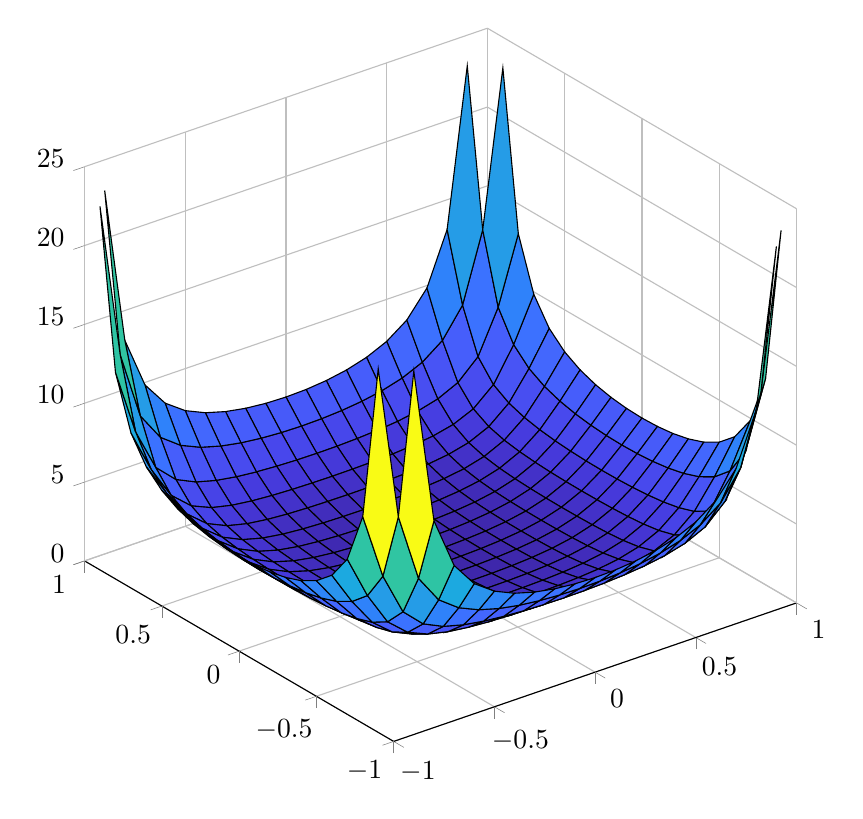
\begin{tikzpicture}

\begin{axis}[%
width=3.56in,
height=3.566in,
at={(0.597in,0.481in)},
scale only axis,
unbounded coords=jump,
xmin=-1,
xmax=1,
tick align=outside,
ymin=-1,
ymax=1,
zmin=0,
zmax=25,
view={-37.5}{30},
axis background/.style={fill=white},
axis x line*=bottom,
axis y line*=left,
axis z line*=left,
xmajorgrids,
ymajorgrids,
zmajorgrids,
legend style={at={(1.03,1)}, anchor=north west, legend cell align=left, align=left, draw=white!15!black}
]

\addplot3[%
surf,
shader=flat corner, draw=black, z buffer=sort, colormap={mymap}{[1pt] rgb(0pt)=(0.2422,0.1504,0.6603); rgb(1pt)=(0.25039,0.164995,0.707614); rgb(2pt)=(0.257771,0.181781,0.751138); rgb(3pt)=(0.264729,0.197757,0.795214); rgb(4pt)=(0.270648,0.214676,0.836371); rgb(5pt)=(0.275114,0.234238,0.870986); rgb(6pt)=(0.2783,0.255871,0.899071); rgb(7pt)=(0.280333,0.278233,0.9221); rgb(8pt)=(0.281338,0.300595,0.941376); rgb(9pt)=(0.281014,0.322757,0.957886); rgb(10pt)=(0.279467,0.344671,0.971676); rgb(11pt)=(0.275971,0.366681,0.982905); rgb(12pt)=(0.269914,0.3892,0.9906); rgb(13pt)=(0.260243,0.412329,0.995157); rgb(14pt)=(0.244033,0.435833,0.998833); rgb(15pt)=(0.220643,0.460257,0.997286); rgb(16pt)=(0.196333,0.484719,0.989152); rgb(17pt)=(0.183405,0.507371,0.979795); rgb(18pt)=(0.178643,0.528857,0.968157); rgb(19pt)=(0.176438,0.549905,0.952019); rgb(20pt)=(0.168743,0.570262,0.935871); rgb(21pt)=(0.154,0.5902,0.9218); rgb(22pt)=(0.146029,0.609119,0.907857); rgb(23pt)=(0.138024,0.627629,0.89729); rgb(24pt)=(0.124814,0.645929,0.888343); rgb(25pt)=(0.111252,0.6635,0.876314); rgb(26pt)=(0.0952095,0.679829,0.859781); rgb(27pt)=(0.0688714,0.694771,0.839357); rgb(28pt)=(0.0296667,0.708167,0.816333); rgb(29pt)=(0.00357143,0.720267,0.7917); rgb(30pt)=(0.00665714,0.731214,0.766014); rgb(31pt)=(0.0433286,0.741095,0.73941); rgb(32pt)=(0.0963952,0.75,0.712038); rgb(33pt)=(0.140771,0.7584,0.684157); rgb(34pt)=(0.1717,0.766962,0.655443); rgb(35pt)=(0.193767,0.775767,0.6251); rgb(36pt)=(0.216086,0.7843,0.5923); rgb(37pt)=(0.246957,0.791795,0.556743); rgb(38pt)=(0.290614,0.79729,0.518829); rgb(39pt)=(0.340643,0.8008,0.478857); rgb(40pt)=(0.3909,0.802871,0.435448); rgb(41pt)=(0.445629,0.802419,0.390919); rgb(42pt)=(0.5044,0.7993,0.348); rgb(43pt)=(0.561562,0.794233,0.304481); rgb(44pt)=(0.617395,0.787619,0.261238); rgb(45pt)=(0.671986,0.779271,0.2227); rgb(46pt)=(0.7242,0.769843,0.191029); rgb(47pt)=(0.773833,0.759805,0.16461); rgb(48pt)=(0.820314,0.749814,0.153529); rgb(49pt)=(0.863433,0.7406,0.159633); rgb(50pt)=(0.903543,0.733029,0.177414); rgb(51pt)=(0.939257,0.728786,0.209957); rgb(52pt)=(0.972757,0.729771,0.239443); rgb(53pt)=(0.995648,0.743371,0.237148); rgb(54pt)=(0.996986,0.765857,0.219943); rgb(55pt)=(0.995205,0.789252,0.202762); rgb(56pt)=(0.9892,0.813567,0.188533); rgb(57pt)=(0.978629,0.838629,0.176557); rgb(58pt)=(0.967648,0.8639,0.16429); rgb(59pt)=(0.96101,0.889019,0.153676); rgb(60pt)=(0.959671,0.913457,0.142257); rgb(61pt)=(0.962795,0.937338,0.12651); rgb(62pt)=(0.969114,0.960629,0.106362); rgb(63pt)=(0.9769,0.9839,0.0805)}, mesh/rows=21]
table[row sep=crcr, point meta=\thisrow{c}] {%
%
x	y	z	c\\
-1	-1	nan	nan\\
-1	-0.9	23.0526315789476	23.0526315789476\\
-1	-0.8	13.111111111111	13.111111111111\\
-1	-0.7	9.84313725490198	9.84313725490198\\
-1	-0.6	8.25	8.25\\
-1	-0.5	7.33333333333333	7.33333333333333\\
-1	-0.4	6.76190476190476	6.76190476190476\\
-1	-0.3	6.3956043956044	6.3956043956044\\
-1	-0.2	6.16666666666667	6.16666666666667\\
-1	-0.1	6.04040404040404	6.04040404040404\\
-1	0	6	6\\
-1	0.1	6.04040404040404	6.04040404040404\\
-1	0.2	6.16666666666667	6.16666666666667\\
-1	0.3	6.3956043956044	6.3956043956044\\
-1	0.4	6.76190476190476	6.76190476190476\\
-1	0.5	7.33333333333333	7.33333333333333\\
-1	0.6	8.25	8.25\\
-1	0.7	9.84313725490198	9.84313725490198\\
-1	0.8	13.111111111111	13.111111111111\\
-1	0.9	23.0526315789476	23.0526315789476\\
-1	1	nan	nan\\
-0.9	-1	23.0526315789474	23.0526315789474\\
-0.9	-0.9	13.2296043018034	13.2296043018034\\
-0.9	-0.8	8.89323388448234	8.89323388448234\\
-0.9	-0.7	7.09420343222335	7.09420343222335\\
-0.9	-0.6	6.14827799579131	6.14827799579131\\
-0.9	-0.5	5.58320204291365	5.58320204291365\\
-0.9	-0.4	5.22320986422556	5.22320986422556\\
-0.9	-0.3	4.98931926341663	4.98931926341663\\
-0.9	-0.2	4.8418995803402	4.8418995803402\\
-0.9	-0.1	4.76018879898449	4.76018879898449\\
-0.9	0	4.73398039226131	4.73398039226131\\
-0.9	0.1	4.76018879898449	4.76018879898449\\
-0.9	0.2	4.8418995803402	4.8418995803402\\
-0.9	0.3	4.98931926341663	4.98931926341663\\
-0.9	0.4	5.22320986422556	5.22320986422556\\
-0.9	0.5	5.58320204291365	5.58320204291365\\
-0.9	0.6	6.14827799579131	6.14827799579131\\
-0.9	0.7	7.09420343222335	7.09420343222335\\
-0.9	0.8	8.89323388448234	8.89323388448234\\
-0.9	0.9	13.2296043018034	13.2296043018034\\
-0.9	1	23.0526315789474	23.0526315789474\\
-0.8	-1	13.1111111111111	13.1111111111111\\
-0.8	-0.9	8.89323388448241	8.89323388448241\\
-0.8	-0.8	6.19988776369148	6.19988776369148\\
-0.8	-0.7	4.9939165246783	4.9939165246783\\
-0.8	-0.6	4.39602375110444	4.39602375110444\\
-0.8	-0.5	4.05755366965927	4.05755366965927\\
-0.8	-0.4	3.84907306567848	3.84907306567848\\
-0.8	-0.3	3.71621993056871	3.71621993056871\\
-0.8	-0.2	3.63337795901121	3.63337795901121\\
-0.8	-0.1	3.58771872965006	3.58771872965006\\
-0.8	0	3.57310898616177	3.57310898616177\\
-0.8	0.1	3.58771872965006	3.58771872965006\\
-0.8	0.2	3.63337795901121	3.63337795901121\\
-0.8	0.3	3.71621993056871	3.71621993056871\\
-0.8	0.4	3.84907306567848	3.84907306567848\\
-0.8	0.5	4.05755366965927	4.05755366965927\\
-0.8	0.6	4.39602375110444	4.39602375110444\\
-0.8	0.7	4.9939165246783	4.9939165246783\\
-0.8	0.8	6.19988776369148	6.19988776369148\\
-0.8	0.9	8.89323388448241	8.89323388448241\\
-0.8	1	13.1111111111111	13.1111111111111\\
-0.7	-1	9.84313725490198	9.84313725490198\\
-0.7	-0.9	7.09420343222336	7.09420343222336\\
-0.7	-0.8	4.99391652467831	4.99391652467831\\
-0.7	-0.7	3.88908128922564	3.88908128922564\\
-0.7	-0.6	3.33774331277907	3.33774331277907\\
-0.7	-0.5	3.04788249518098	3.04788249518098\\
-0.7	-0.4	2.88518758693567	2.88518758693567\\
-0.7	-0.3	2.78981199902195	2.78981199902195\\
-0.7	-0.2	2.73402424622654	2.73402424622654\\
-0.7	-0.1	2.70454808009259	2.70454808009259\\
-0.7	0	2.69531099391084	2.69531099391084\\
-0.7	0.1	2.70454808009259	2.70454808009259\\
-0.7	0.2	2.73402424622654	2.73402424622654\\
-0.7	0.3	2.78981199902195	2.78981199902195\\
-0.7	0.4	2.88518758693567	2.88518758693567\\
-0.7	0.5	3.04788249518098	3.04788249518098\\
-0.7	0.6	3.33774331277907	3.33774331277907\\
-0.7	0.7	3.88908128922564	3.88908128922564\\
-0.7	0.8	4.99391652467831	4.99391652467831\\
-0.7	0.9	7.09420343222336	7.09420343222336\\
-0.7	1	9.84313725490198	9.84313725490198\\
-0.6	-1	8.24999999999999	8.24999999999999\\
-0.6	-0.9	6.14827799579132	6.14827799579132\\
-0.6	-0.8	4.39602375110444	4.39602375110444\\
-0.6	-0.7	3.33774331277907	3.33774331277907\\
-0.6	-0.6	2.76256313292354	2.76256313292354\\
-0.6	-0.5	2.45286827306655	2.45286827306655\\
-0.6	-0.4	2.28240657625557	2.28240657625557\\
-0.6	-0.3	2.18662860979927	2.18662860979927\\
-0.6	-0.2	2.13322049347278	2.13322049347278\\
-0.6	-0.1	2.10609862401655	2.10609862401655\\
-0.6	0	2.09778596995664	2.09778596995664\\
-0.6	0.1	2.10609862401655	2.10609862401655\\
-0.6	0.2	2.13322049347278	2.13322049347278\\
-0.6	0.3	2.18662860979927	2.18662860979927\\
-0.6	0.4	2.28240657625557	2.28240657625557\\
-0.6	0.5	2.45286827306655	2.45286827306655\\
-0.6	0.6	2.76256313292354	2.76256313292354\\
-0.6	0.7	3.33774331277907	3.33774331277907\\
-0.6	0.8	4.39602375110444	4.39602375110444\\
-0.6	0.9	6.14827799579132	6.14827799579132\\
-0.6	1	8.24999999999999	8.24999999999999\\
-0.5	-1	7.33333333333333	7.33333333333333\\
-0.5	-0.9	5.58320204291365	5.58320204291365\\
-0.5	-0.8	4.05755366965926	4.05755366965926\\
-0.5	-0.7	3.04788249518098	3.04788249518098\\
-0.5	-0.6	2.45286827306655	2.45286827306655\\
-0.5	-0.5	2.11438191683587	2.11438191683587\\
-0.5	-0.4	1.92230810937407	1.92230810937407\\
-0.5	-0.3	1.81309357845656	1.81309357845656\\
-0.5	-0.2	1.75218118209068	1.75218118209068\\
-0.5	-0.1	1.72139668275897	1.72139668275897\\
-0.5	0	1.712	1.712\\
-0.5	0.1	1.72139668275897	1.72139668275897\\
-0.5	0.2	1.75218118209068	1.75218118209068\\
-0.5	0.3	1.81309357845656	1.81309357845656\\
-0.5	0.4	1.92230810937407	1.92230810937407\\
-0.5	0.5	2.11438191683587	2.11438191683587\\
-0.5	0.6	2.45286827306655	2.45286827306655\\
-0.5	0.7	3.04788249518098	3.04788249518098\\
-0.5	0.8	4.05755366965926	4.05755366965926\\
-0.5	0.9	5.58320204291365	5.58320204291365\\
-0.5	1	7.33333333333333	7.33333333333333\\
-0.4	-1	6.76190476190476	6.76190476190476\\
-0.4	-0.9	5.22320986422556	5.22320986422556\\
-0.4	-0.8	3.84907306567848	3.84907306567848\\
-0.4	-0.7	2.88518758693567	2.88518758693567\\
-0.4	-0.6	2.28240657625558	2.28240657625558\\
-0.4	-0.5	1.92230810937407	1.92230810937407\\
-0.4	-0.4	1.71032089901499	1.71032089901499\\
-0.4	-0.3	1.58660034951018	1.58660034951018\\
-0.4	-0.2	1.51638590795481	1.51638590795481\\
-0.4	-0.1	1.48052510090217	1.48052510090217\\
-0.4	0	1.46952499618196	1.46952499618196\\
-0.4	0.1	1.48052510090217	1.48052510090217\\
-0.4	0.2	1.51638590795481	1.51638590795481\\
-0.4	0.3	1.58660034951018	1.58660034951018\\
-0.4	0.4	1.71032089901499	1.71032089901499\\
-0.4	0.5	1.92230810937407	1.92230810937407\\
-0.4	0.6	2.28240657625558	2.28240657625558\\
-0.4	0.7	2.88518758693567	2.88518758693567\\
-0.4	0.8	3.84907306567848	3.84907306567848\\
-0.4	0.9	5.22320986422556	5.22320986422556\\
-0.4	1	6.76190476190476	6.76190476190476\\
-0.3	-1	6.3956043956044	6.3956043956044\\
-0.3	-0.9	4.98931926341663	4.98931926341663\\
-0.3	-0.8	3.71621993056871	3.71621993056871\\
-0.3	-0.7	2.78981199902195	2.78981199902195\\
-0.3	-0.6	2.18662860979928	2.18662860979928\\
-0.3	-0.5	1.81309357845656	1.81309357845656\\
-0.3	-0.4	1.58660034951018	1.58660034951018\\
-0.3	-0.3	1.45130742605288	1.45130742605288\\
-0.3	-0.2	1.3731816152005	1.3731816152005\\
-0.3	-0.1	1.33281170445424	1.33281170445424\\
-0.3	0	1.32035502909706	1.32035502909706\\
-0.3	0.1	1.33281170445424	1.33281170445424\\
-0.3	0.2	1.3731816152005	1.3731816152005\\
-0.3	0.3	1.45130742605288	1.45130742605288\\
-0.3	0.4	1.58660034951018	1.58660034951018\\
-0.3	0.5	1.81309357845656	1.81309357845656\\
-0.3	0.6	2.18662860979928	2.18662860979928\\
-0.3	0.7	2.78981199902195	2.78981199902195\\
-0.3	0.8	3.71621993056871	3.71621993056871\\
-0.3	0.9	4.98931926341663	4.98931926341663\\
-0.3	1	6.3956043956044	6.3956043956044\\
-0.2	-1	6.16666666666667	6.16666666666667\\
-0.2	-0.9	4.8418995803402	4.8418995803402\\
-0.2	-0.8	3.63337795901121	3.63337795901121\\
-0.2	-0.7	2.73402424622654	2.73402424622654\\
-0.2	-0.6	2.13322049347279	2.13322049347279\\
-0.2	-0.5	1.75218118209068	1.75218118209068\\
-0.2	-0.4	1.51638590795481	1.51638590795481\\
-0.2	-0.3	1.37318161520051	1.37318161520051\\
-0.2	-0.2	1.28942400545157	1.28942400545157\\
-0.2	-0.1	1.24576115741349	1.24576115741349\\
-0.2	0	1.23222725701503	1.23222725701503\\
-0.2	0.1	1.24576115741349	1.24576115741349\\
-0.2	0.2	1.28942400545157	1.28942400545157\\
-0.2	0.3	1.37318161520051	1.37318161520051\\
-0.2	0.4	1.51638590795481	1.51638590795481\\
-0.2	0.5	1.75218118209068	1.75218118209068\\
-0.2	0.6	2.13322049347279	2.13322049347279\\
-0.2	0.7	2.73402424622654	2.73402424622654\\
-0.2	0.8	3.63337795901121	3.63337795901121\\
-0.2	0.9	4.8418995803402	4.8418995803402\\
-0.2	1	6.16666666666667	6.16666666666667\\
-0.1	-1	6.04040404040404	6.04040404040404\\
-0.1	-0.9	4.76018879898449	4.76018879898449\\
-0.1	-0.8	3.58771872965006	3.58771872965006\\
-0.1	-0.7	2.70454808009259	2.70454808009259\\
-0.1	-0.6	2.10609862401655	2.10609862401655\\
-0.1	-0.5	1.72139668275897	1.72139668275897\\
-0.1	-0.4	1.48052510090217	1.48052510090217\\
-0.1	-0.3	1.33281170445424	1.33281170445424\\
-0.1	-0.2	1.24576115741349	1.24576115741349\\
-0.1	-0.1	1.20014284621084	1.20014284621084\\
-0.1	0	1.1859644491566	1.1859644491566\\
-0.1	0.1	1.20014284621084	1.20014284621084\\
-0.1	0.2	1.24576115741349	1.24576115741349\\
-0.1	0.3	1.33281170445424	1.33281170445424\\
-0.1	0.4	1.48052510090217	1.48052510090217\\
-0.1	0.5	1.72139668275897	1.72139668275897\\
-0.1	0.6	2.10609862401655	2.10609862401655\\
-0.1	0.7	2.70454808009259	2.70454808009259\\
-0.1	0.8	3.58771872965006	3.58771872965006\\
-0.1	0.9	4.76018879898449	4.76018879898449\\
-0.1	1	6.04040404040404	6.04040404040404\\
0	-1	6	6\\
0	-0.9	4.73398039226131	4.73398039226131\\
0	-0.8	3.57310898616177	3.57310898616177\\
0	-0.7	2.69531099391084	2.69531099391084\\
0	-0.6	2.09778596995664	2.09778596995664\\
0	-0.5	1.712	1.712\\
0	-0.4	1.46952499618196	1.46952499618196\\
0	-0.3	1.32035502909706	1.32035502909706\\
0	-0.2	1.23222725701503	1.23222725701503\\
0	-0.1	1.1859644491566	1.1859644491566\\
0	0	1.17157287525381	1.17157287525381\\
0	0.1	1.1859644491566	1.1859644491566\\
0	0.2	1.23222725701503	1.23222725701503\\
0	0.3	1.32035502909706	1.32035502909706\\
0	0.4	1.46952499618196	1.46952499618196\\
0	0.5	1.712	1.712\\
0	0.6	2.09778596995664	2.09778596995664\\
0	0.7	2.69531099391084	2.69531099391084\\
0	0.8	3.57310898616177	3.57310898616177\\
0	0.9	4.73398039226131	4.73398039226131\\
0	1	6	6\\
0.1	-1	6.04040404040404	6.04040404040404\\
0.1	-0.9	4.76018879898449	4.76018879898449\\
0.1	-0.8	3.58771872965006	3.58771872965006\\
0.1	-0.7	2.70454808009259	2.70454808009259\\
0.1	-0.6	2.10609862401655	2.10609862401655\\
0.1	-0.5	1.72139668275897	1.72139668275897\\
0.1	-0.4	1.48052510090217	1.48052510090217\\
0.1	-0.3	1.33281170445424	1.33281170445424\\
0.1	-0.2	1.24576115741349	1.24576115741349\\
0.1	-0.1	1.20014284621084	1.20014284621084\\
0.1	0	1.1859644491566	1.1859644491566\\
0.1	0.1	1.20014284621084	1.20014284621084\\
0.1	0.2	1.24576115741349	1.24576115741349\\
0.1	0.3	1.33281170445424	1.33281170445424\\
0.1	0.4	1.48052510090217	1.48052510090217\\
0.1	0.5	1.72139668275897	1.72139668275897\\
0.1	0.6	2.10609862401655	2.10609862401655\\
0.1	0.7	2.70454808009259	2.70454808009259\\
0.1	0.8	3.58771872965006	3.58771872965006\\
0.1	0.9	4.76018879898449	4.76018879898449\\
0.1	1	6.04040404040404	6.04040404040404\\
0.2	-1	6.16666666666667	6.16666666666667\\
0.2	-0.9	4.8418995803402	4.8418995803402\\
0.2	-0.8	3.63337795901121	3.63337795901121\\
0.2	-0.7	2.73402424622654	2.73402424622654\\
0.2	-0.6	2.13322049347279	2.13322049347279\\
0.2	-0.5	1.75218118209068	1.75218118209068\\
0.2	-0.4	1.51638590795481	1.51638590795481\\
0.2	-0.3	1.37318161520051	1.37318161520051\\
0.2	-0.2	1.28942400545157	1.28942400545157\\
0.2	-0.1	1.24576115741349	1.24576115741349\\
0.2	0	1.23222725701503	1.23222725701503\\
0.2	0.1	1.24576115741349	1.24576115741349\\
0.2	0.2	1.28942400545157	1.28942400545157\\
0.2	0.3	1.37318161520051	1.37318161520051\\
0.2	0.4	1.51638590795481	1.51638590795481\\
0.2	0.5	1.75218118209068	1.75218118209068\\
0.2	0.6	2.13322049347279	2.13322049347279\\
0.2	0.7	2.73402424622654	2.73402424622654\\
0.2	0.8	3.63337795901121	3.63337795901121\\
0.2	0.9	4.8418995803402	4.8418995803402\\
0.2	1	6.16666666666667	6.16666666666667\\
0.3	-1	6.3956043956044	6.3956043956044\\
0.3	-0.9	4.98931926341663	4.98931926341663\\
0.3	-0.8	3.71621993056871	3.71621993056871\\
0.3	-0.7	2.78981199902195	2.78981199902195\\
0.3	-0.6	2.18662860979928	2.18662860979928\\
0.3	-0.5	1.81309357845656	1.81309357845656\\
0.3	-0.4	1.58660034951018	1.58660034951018\\
0.3	-0.3	1.45130742605288	1.45130742605288\\
0.3	-0.2	1.3731816152005	1.3731816152005\\
0.3	-0.1	1.33281170445424	1.33281170445424\\
0.3	0	1.32035502909706	1.32035502909706\\
0.3	0.1	1.33281170445424	1.33281170445424\\
0.3	0.2	1.3731816152005	1.3731816152005\\
0.3	0.3	1.45130742605288	1.45130742605288\\
0.3	0.4	1.58660034951018	1.58660034951018\\
0.3	0.5	1.81309357845656	1.81309357845656\\
0.3	0.6	2.18662860979928	2.18662860979928\\
0.3	0.7	2.78981199902195	2.78981199902195\\
0.3	0.8	3.71621993056871	3.71621993056871\\
0.3	0.9	4.98931926341663	4.98931926341663\\
0.3	1	6.3956043956044	6.3956043956044\\
0.4	-1	6.76190476190476	6.76190476190476\\
0.4	-0.9	5.22320986422556	5.22320986422556\\
0.4	-0.8	3.84907306567848	3.84907306567848\\
0.4	-0.7	2.88518758693567	2.88518758693567\\
0.4	-0.6	2.28240657625558	2.28240657625558\\
0.4	-0.5	1.92230810937407	1.92230810937407\\
0.4	-0.4	1.71032089901499	1.71032089901499\\
0.4	-0.3	1.58660034951018	1.58660034951018\\
0.4	-0.2	1.51638590795481	1.51638590795481\\
0.4	-0.1	1.48052510090217	1.48052510090217\\
0.4	0	1.46952499618196	1.46952499618196\\
0.4	0.1	1.48052510090217	1.48052510090217\\
0.4	0.2	1.51638590795481	1.51638590795481\\
0.4	0.3	1.58660034951018	1.58660034951018\\
0.4	0.4	1.71032089901499	1.71032089901499\\
0.4	0.5	1.92230810937407	1.92230810937407\\
0.4	0.6	2.28240657625558	2.28240657625558\\
0.4	0.7	2.88518758693567	2.88518758693567\\
0.4	0.8	3.84907306567848	3.84907306567848\\
0.4	0.9	5.22320986422556	5.22320986422556\\
0.4	1	6.76190476190476	6.76190476190476\\
0.5	-1	7.33333333333333	7.33333333333333\\
0.5	-0.9	5.58320204291365	5.58320204291365\\
0.5	-0.8	4.05755366965926	4.05755366965926\\
0.5	-0.7	3.04788249518098	3.04788249518098\\
0.5	-0.6	2.45286827306655	2.45286827306655\\
0.5	-0.5	2.11438191683587	2.11438191683587\\
0.5	-0.4	1.92230810937407	1.92230810937407\\
0.5	-0.3	1.81309357845656	1.81309357845656\\
0.5	-0.2	1.75218118209068	1.75218118209068\\
0.5	-0.1	1.72139668275897	1.72139668275897\\
0.5	0	1.712	1.712\\
0.5	0.1	1.72139668275897	1.72139668275897\\
0.5	0.2	1.75218118209068	1.75218118209068\\
0.5	0.3	1.81309357845656	1.81309357845656\\
0.5	0.4	1.92230810937407	1.92230810937407\\
0.5	0.5	2.11438191683587	2.11438191683587\\
0.5	0.6	2.45286827306655	2.45286827306655\\
0.5	0.7	3.04788249518098	3.04788249518098\\
0.5	0.8	4.05755366965926	4.05755366965926\\
0.5	0.9	5.58320204291365	5.58320204291365\\
0.5	1	7.33333333333333	7.33333333333333\\
0.6	-1	8.24999999999999	8.24999999999999\\
0.6	-0.9	6.14827799579132	6.14827799579132\\
0.6	-0.8	4.39602375110444	4.39602375110444\\
0.6	-0.7	3.33774331277907	3.33774331277907\\
0.6	-0.6	2.76256313292354	2.76256313292354\\
0.6	-0.5	2.45286827306655	2.45286827306655\\
0.6	-0.4	2.28240657625557	2.28240657625557\\
0.6	-0.3	2.18662860979927	2.18662860979927\\
0.6	-0.2	2.13322049347278	2.13322049347278\\
0.6	-0.1	2.10609862401655	2.10609862401655\\
0.6	0	2.09778596995664	2.09778596995664\\
0.6	0.1	2.10609862401655	2.10609862401655\\
0.6	0.2	2.13322049347278	2.13322049347278\\
0.6	0.3	2.18662860979927	2.18662860979927\\
0.6	0.4	2.28240657625557	2.28240657625557\\
0.6	0.5	2.45286827306655	2.45286827306655\\
0.6	0.6	2.76256313292354	2.76256313292354\\
0.6	0.7	3.33774331277907	3.33774331277907\\
0.6	0.8	4.39602375110444	4.39602375110444\\
0.6	0.9	6.14827799579132	6.14827799579132\\
0.6	1	8.24999999999999	8.24999999999999\\
0.7	-1	9.84313725490198	9.84313725490198\\
0.7	-0.9	7.09420343222336	7.09420343222336\\
0.7	-0.8	4.99391652467831	4.99391652467831\\
0.7	-0.7	3.88908128922564	3.88908128922564\\
0.7	-0.6	3.33774331277907	3.33774331277907\\
0.7	-0.5	3.04788249518098	3.04788249518098\\
0.7	-0.4	2.88518758693567	2.88518758693567\\
0.7	-0.3	2.78981199902195	2.78981199902195\\
0.7	-0.2	2.73402424622654	2.73402424622654\\
0.7	-0.1	2.70454808009259	2.70454808009259\\
0.7	0	2.69531099391084	2.69531099391084\\
0.7	0.1	2.70454808009259	2.70454808009259\\
0.7	0.2	2.73402424622654	2.73402424622654\\
0.7	0.3	2.78981199902195	2.78981199902195\\
0.7	0.4	2.88518758693567	2.88518758693567\\
0.7	0.5	3.04788249518098	3.04788249518098\\
0.7	0.6	3.33774331277907	3.33774331277907\\
0.7	0.7	3.88908128922564	3.88908128922564\\
0.7	0.8	4.99391652467831	4.99391652467831\\
0.7	0.9	7.09420343222336	7.09420343222336\\
0.7	1	9.84313725490198	9.84313725490198\\
0.8	-1	13.1111111111111	13.1111111111111\\
0.8	-0.9	8.89323388448241	8.89323388448241\\
0.8	-0.8	6.19988776369148	6.19988776369148\\
0.8	-0.7	4.9939165246783	4.9939165246783\\
0.8	-0.6	4.39602375110444	4.39602375110444\\
0.8	-0.5	4.05755366965927	4.05755366965927\\
0.8	-0.4	3.84907306567848	3.84907306567848\\
0.8	-0.3	3.71621993056871	3.71621993056871\\
0.8	-0.2	3.63337795901121	3.63337795901121\\
0.8	-0.1	3.58771872965006	3.58771872965006\\
0.8	0	3.57310898616177	3.57310898616177\\
0.8	0.1	3.58771872965006	3.58771872965006\\
0.8	0.2	3.63337795901121	3.63337795901121\\
0.8	0.3	3.71621993056871	3.71621993056871\\
0.8	0.4	3.84907306567848	3.84907306567848\\
0.8	0.5	4.05755366965927	4.05755366965927\\
0.8	0.6	4.39602375110444	4.39602375110444\\
0.8	0.7	4.9939165246783	4.9939165246783\\
0.8	0.8	6.19988776369148	6.19988776369148\\
0.8	0.9	8.89323388448241	8.89323388448241\\
0.8	1	13.1111111111111	13.1111111111111\\
0.9	-1	23.0526315789474	23.0526315789474\\
0.9	-0.9	13.2296043018034	13.2296043018034\\
0.9	-0.8	8.89323388448234	8.89323388448234\\
0.9	-0.7	7.09420343222335	7.09420343222335\\
0.9	-0.6	6.14827799579131	6.14827799579131\\
0.9	-0.5	5.58320204291365	5.58320204291365\\
0.9	-0.4	5.22320986422556	5.22320986422556\\
0.9	-0.3	4.98931926341663	4.98931926341663\\
0.9	-0.2	4.8418995803402	4.8418995803402\\
0.9	-0.1	4.76018879898449	4.76018879898449\\
0.9	0	4.73398039226131	4.73398039226131\\
0.9	0.1	4.76018879898449	4.76018879898449\\
0.9	0.2	4.8418995803402	4.8418995803402\\
0.9	0.3	4.98931926341663	4.98931926341663\\
0.9	0.4	5.22320986422556	5.22320986422556\\
0.9	0.5	5.58320204291365	5.58320204291365\\
0.9	0.6	6.14827799579131	6.14827799579131\\
0.9	0.7	7.09420343222335	7.09420343222335\\
0.9	0.8	8.89323388448234	8.89323388448234\\
0.9	0.9	13.2296043018034	13.2296043018034\\
0.9	1	23.0526315789474	23.0526315789474\\
1	-1	nan	nan\\
1	-0.9	23.0526315789476	23.0526315789476\\
1	-0.8	13.111111111111	13.111111111111\\
1	-0.7	9.84313725490198	9.84313725490198\\
1	-0.6	8.25	8.25\\
1	-0.5	7.33333333333333	7.33333333333333\\
1	-0.4	6.76190476190476	6.76190476190476\\
1	-0.3	6.3956043956044	6.3956043956044\\
1	-0.2	6.16666666666667	6.16666666666667\\
1	-0.1	6.04040404040404	6.04040404040404\\
1	0	6	6\\
1	0.1	6.04040404040404	6.04040404040404\\
1	0.2	6.16666666666667	6.16666666666667\\
1	0.3	6.3956043956044	6.3956043956044\\
1	0.4	6.76190476190476	6.76190476190476\\
1	0.5	7.33333333333333	7.33333333333333\\
1	0.6	8.25	8.25\\
1	0.7	9.84313725490198	9.84313725490198\\
1	0.8	13.111111111111	13.111111111111\\
1	0.9	23.0526315789476	23.0526315789476\\
1	1	nan	nan\\
};
%\addlegendentry{data1}

\end{axis}
\end{tikzpicture}%
}
\caption{Negativer Laplace der Gewichtsfunktion}
\label{fig:Gewicht}
\end{figure}
Als weiteres Indiz für die Ursache des Fehlers betrachten wir die zweite \ac{PDE}. In dem Fall ist der negative Laplace der Gewichtsfunktion gegeben durch
\begin{align*}
- \Delta w(x) = 4
\end{align*}
und hat damit keine Singularitäten.

Tatsächlich erhalten wir, wenn wir den Testfehler der zweiten \ac{PDE} in Abbildung \ref{fig:error-grid-both} betrachten, ein komplett anderes Bild. Alle Verfahren erreichen mit spätestens $200$ Kollokationspunkten ihre besten Ergebnisse. Die gewichteten Verfahren erreichen dieses Mal einen Testfehler von $10^{-8}$ und $10^{-9}$ für das nicht-symmetrische beziehungsweise symmetrische Verfahren und sind damit besser als die Standardverfahren, welche nur einen Testfehler von $10^{-7}$ und $10^{-8}$ für das nicht-symmetrische beziehungsweise symmetrische Verfahren erreichen. Demnach sollten wir bei der Wahl der Gewichtsfunktionen darauf achten, dass in diesen und deren partiellen Ableitungen keine Singularitäten entstehen.

\subsubsection{Zufällige Kollokationspunkte}
Als nächstes schauen wir uns zufällig verteilte Kollokationspunkte an. In Abbildung \ref{fig:error-random} ist der Fehler bei unterschiedlich vielen zufällig verteilten Kollokationspunkten für beide \acp{PDE} dargestellt.
\begin{figure}[ht]
\centering
\resizebox {\columnwidth} {!} {
% This file was created by matlab2tikz.
%
%The latest updates can be retrieved from
%  http://www.mathworks.com/matlabcentral/fileexchange/22022-matlab2tikz-matlab2tikz
%where you can also make suggestions and rate matlab2tikz.
%
\definecolor{mycolor1}{rgb}{0.00000,0.44700,0.74100}%
\definecolor{mycolor2}{rgb}{0.85000,0.32500,0.09800}%
\definecolor{mycolor3}{rgb}{0.92900,0.69400,0.12500}%
\definecolor{mycolor4}{rgb}{0.49400,0.18400,0.55600}%
%
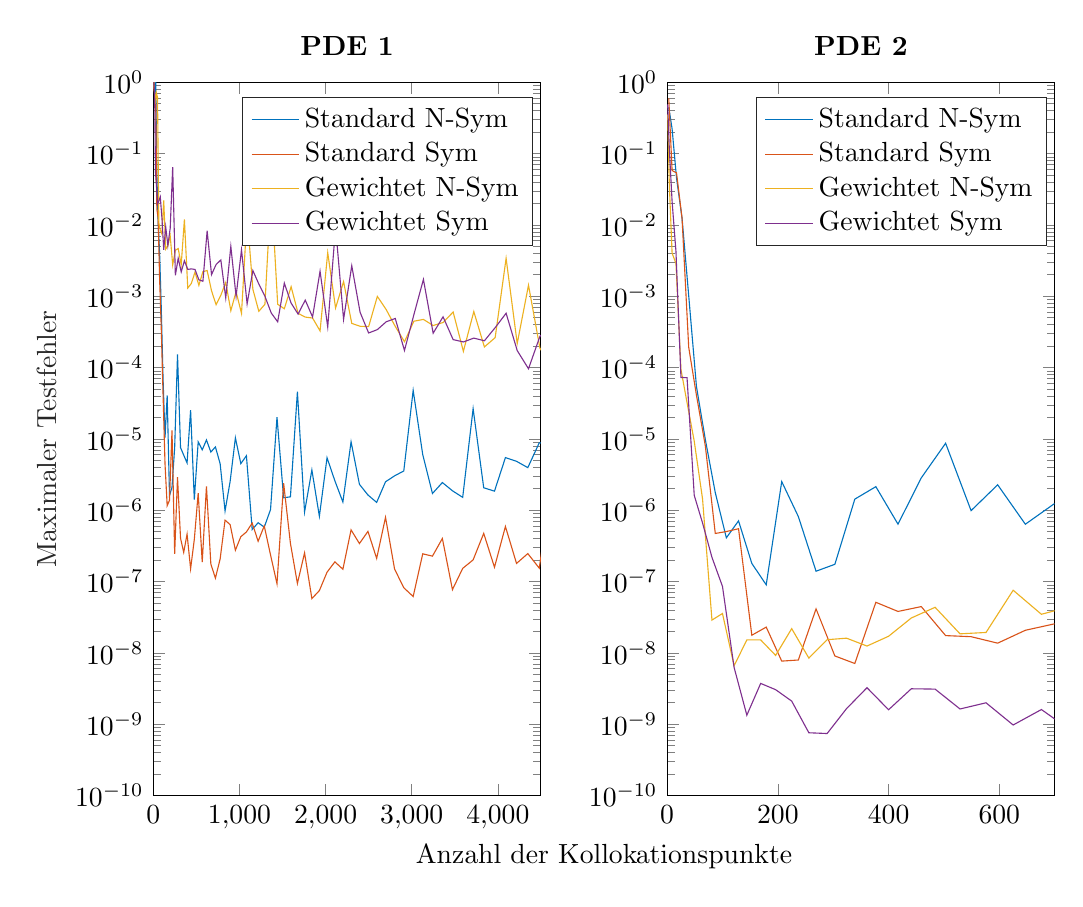
\begin{tikzpicture}

\begin{axis}[%
name = ax1,
width=1.938in,
height=3.566in,
at={(0.758in,0.481in)},
scale only axis,
xmin=0,
xmax=4500,
%xlabel style={font=\color{white!15!black}},
%xlabel={amount of collocation points},
ymode=log,
ymin=1e-10,
ymax=1,
yminorticks=true,
ylabel style={font=\color{white!15!black}},
ylabel={Maximaler Testfehler},
axis background/.style={fill=white},
title style={font=\bfseries},
title={\ac{PDE} 1},
legend style={legend cell align=left, align=left, draw=white!15!black}
]
\addplot [color=mycolor1]
  table[row sep=crcr]{%
4	0.999748271191593\\
8	1.08133089295795\\
17	0.787488457043724\\
28	1.00876021033637\\
41	0.0527639218376913\\
56	0.0109041187286126\\
73	0.00406914619466443\\
92	0.000718967326502562\\
113	7.14934437407964e-05\\
136	1.0394229939939e-05\\
161	4.05968459937789e-05\\
188	1.59883979566899e-06\\
217	2.10279376054723e-06\\
248	7.56134738222336e-06\\
281	0.000153039106389988\\
316	7.55029009213981e-06\\
353	5.91196770269309e-06\\
392	4.59954539053925e-06\\
433	2.53142893736902e-05\\
476	1.4072184219005e-06\\
521	9.0805385786763e-06\\
568	7.02877939401381e-06\\
617	9.65326440827141e-06\\
668	6.53233612457615e-06\\
721	7.71608473371099e-06\\
776	4.47640278899986e-06\\
833	9.75911040312916e-07\\
892	2.536628800065e-06\\
953	1.03296259561514e-05\\
1016	4.49691019682036e-06\\
1081	5.79796909065677e-06\\
1148	5.36176315985015e-07\\
1217	6.67522949859833e-07\\
1288	5.7846619649915e-07\\
1361	1.02039667068676e-06\\
1436	2.01015942932758e-05\\
1513	1.49408012528607e-06\\
1592	1.53918436382461e-06\\
1673	4.58170527043722e-05\\
1756	9.44525468289659e-07\\
1841	3.6672603868082e-06\\
1928	8.21270517814554e-07\\
2017	5.44312765882182e-06\\
2108	2.58230115202096e-06\\
2201	1.30267089670788e-06\\
2296	9.10570958706503e-06\\
2393	2.30663158780342e-06\\
2492	1.63296681199299e-06\\
2593	1.28691629730504e-06\\
2696	2.50154829639637e-06\\
2801	3.03184176456139e-06\\
2908	3.54799379120863e-06\\
3017	4.79236326328715e-05\\
3128	6.02316715461737e-06\\
3241	1.7150268772359e-06\\
3356	2.44308890073874e-06\\
3473	1.87183747790698e-06\\
3592	1.51433275658031e-06\\
3713	2.6559932695791e-05\\
3836	2.06367698421528e-06\\
3961	1.84961640375958e-06\\
4088	5.45725167756111e-06\\
4217	4.84476203710393e-06\\
4348	3.95186519672186e-06\\
4481	8.80961123095325e-06\\
4616	8.48670397762818e-06\\
4753	3.75712176366172e-06\\
4892	2.6954752167796e-06\\
5033	1.11269877450804e-05\\
5176	4.55647059260933e-06\\
};
\addlegendentry{Standard N-Sym}

\addplot [color=mycolor2]
  table[row sep=crcr]{%
4	1.05433617432393\\
8	1.00032665947363\\
17	0.656244606477592\\
28	0.488123125287577\\
41	0.0167595794262468\\
56	0.0126425780735455\\
73	0.00176754336468821\\
92	0.000367559673635359\\
113	4.29232002490121e-05\\
136	4.42396413366519e-06\\
161	1.15774510173888e-06\\
188	1.37540730423685e-06\\
217	1.31405627492309e-05\\
248	2.4364927175835e-07\\
281	2.91152883069579e-06\\
316	4.04687917843205e-07\\
353	2.56703371314879e-07\\
392	4.61335609117097e-07\\
433	1.50778136864815e-07\\
476	3.88877087864614e-07\\
521	1.73850616269622e-06\\
568	1.86488130382578e-07\\
617	2.16339936420784e-06\\
668	1.75947158773115e-07\\
721	1.11544479042269e-07\\
776	2.07809496832745e-07\\
833	7.25611153162831e-07\\
892	6.27616288162436e-07\\
953	2.748787992779e-07\\
1016	4.25056406849755e-07\\
1081	4.95227150620892e-07\\
1148	6.60296271215444e-07\\
1217	3.6682225745821e-07\\
1288	6.01276105682835e-07\\
1361	2.35795907965741e-07\\
1436	9.30683431432655e-08\\
1513	2.39172673632826e-06\\
1592	3.42675820719229e-07\\
1673	9.38543386896917e-08\\
1756	2.5195072017592e-07\\
1841	5.76603644275586e-08\\
1928	7.46185584432624e-08\\
2017	1.35019466940278e-07\\
2108	1.8868877105227e-07\\
2201	1.48583618297948e-07\\
2296	5.29822003408897e-07\\
2393	3.40882660987418e-07\\
2492	5.04456426075883e-07\\
2593	2.10858148497195e-07\\
2696	7.93952114386265e-07\\
2801	1.4973639728133e-07\\
2908	8.17716342416119e-08\\
3017	6.1614441659863e-08\\
3128	2.44505821644925e-07\\
3241	2.26950638240742e-07\\
3356	4.01392113436039e-07\\
3473	7.69048774384995e-08\\
3592	1.52800960995236e-07\\
3713	2.01101086172439e-07\\
3836	4.73264991585065e-07\\
3961	1.58538790109852e-07\\
4088	5.90692866953013e-07\\
4217	1.7937911950261e-07\\
4348	2.46416590243825e-07\\
4481	1.53934107016696e-07\\
4616	2.18499662774096e-06\\
4753	2.78608662418467e-07\\
4892	2.08882456109727e-07\\
5033	1.68740294043124e-07\\
5176	1.25164081876683e-07\\
};
\addlegendentry{Standard Sym}

\addplot [color=mycolor3]
  table[row sep=crcr]{%
1	0.999748271191593\\
4	1.03142995437141\\
9	0.786116020859602\\
16	0.698872819735042\\
25	0.498915530291019\\
36	0.704722863175288\\
49	0.611470544068062\\
64	0.0106738238431806\\
81	0.00846406069694688\\
100	0.00742702542881313\\
121	0.0220102197149016\\
144	0.00457905440007705\\
169	0.00509467696278077\\
196	0.00703727304792809\\
225	0.00275120602099829\\
256	0.00441701737535992\\
289	0.00465806280572194\\
324	0.00276982772256065\\
361	0.0119481788398219\\
400	0.0013025263291274\\
441	0.00150669209981602\\
484	0.00217431067039899\\
529	0.00142201113861514\\
576	0.00221446456739976\\
625	0.00229094071132841\\
676	0.00119147529800234\\
729	0.000760281316827064\\
784	0.00103444806041601\\
841	0.0015600464205178\\
900	0.000626061907849821\\
961	0.00116075147651149\\
1024	0.000574065659955769\\
1089	0.0139310302097414\\
1156	0.00125073043455332\\
1225	0.000614581607711058\\
1296	0.000771687936694524\\
1369	0.0323749440009249\\
1444	0.000771991882251997\\
1521	0.000667891788862378\\
1600	0.00136046576912181\\
1681	0.000575470048991611\\
1764	0.000509889359674848\\
1849	0.000494766928465637\\
1936	0.000326558650546049\\
2025	0.00409080886488526\\
2116	0.000683812958245712\\
2209	0.00160371191726705\\
2304	0.000416075642606605\\
2401	0.000378952038433874\\
2500	0.000375028573406606\\
2601	0.000994625347152934\\
2704	0.000648966992822002\\
2809	0.000377421073108503\\
2916	0.000230095434709553\\
3025	0.000446172265639669\\
3136	0.000473324088424341\\
3249	0.000388508917245289\\
3364	0.000428032326772952\\
3481	0.000600606273141508\\
3600	0.000168717166663334\\
3721	0.000610215630281838\\
3844	0.000194586140408712\\
3969	0.000262959694313019\\
4096	0.00339953340739552\\
4225	0.000217113422204502\\
4356	0.00142888916798941\\
4489	0.000186455191880302\\
4624	0.000105405074523164\\
4761	0.000120611474983484\\
4900	0.000294025473507657\\
};
\addlegendentry{Gewichtet N-Sym}

\addplot [color=mycolor4]
  table[row sep=crcr]{%
1	0.999748271316304\\
4	0.999751384039337\\
9	0.909898599105437\\
16	0.620209403865854\\
25	0.0552234781086134\\
36	0.0362275171015879\\
49	0.0196258567645095\\
64	0.0216036616652308\\
81	0.0247118634926999\\
100	0.0125138003782383\\
121	0.00448730606378703\\
144	0.00939115922034597\\
169	0.00515212576558964\\
196	0.00894824020274193\\
225	0.0646436951925821\\
256	0.00196464535749688\\
289	0.00339906857097611\\
324	0.0021932638177733\\
361	0.0031423359427928\\
400	0.00237622812186326\\
441	0.00241798730992757\\
484	0.00237566816076224\\
529	0.00169974181119393\\
576	0.00162260594098848\\
625	0.00827509565468709\\
676	0.00201132129394521\\
729	0.00278213638848089\\
784	0.00322462890469077\\
841	0.000948345293616704\\
900	0.00499508125593828\\
961	0.000998783694139487\\
1024	0.00448608434440878\\
1089	0.000781102586880324\\
1156	0.00229222336556234\\
1225	0.00148211327985577\\
1296	0.000997588225633176\\
1369	0.000582902483207319\\
1444	0.000437834934091825\\
1521	0.00152806931504255\\
1600	0.000800994834489036\\
1681	0.000562049065303371\\
1764	0.000882555882422174\\
1849	0.000512296497525365\\
1936	0.00224544147747302\\
2025	0.000369847864830112\\
2116	0.0093295862010786\\
2209	0.000473890181991663\\
2304	0.00267560699936579\\
2401	0.000594623759577819\\
2500	0.000305277012374761\\
2601	0.000340357778171917\\
2704	0.000438210062154924\\
2809	0.000488154184416247\\
2916	0.00017351179575468\\
3025	0.000549801875980989\\
3136	0.00172170826323831\\
3249	0.000303202374866997\\
3364	0.000514541524357098\\
3481	0.000246569794449477\\
3600	0.000228484768325403\\
3721	0.000258760050246464\\
3844	0.000237294328006663\\
3969	0.000362760651774334\\
4096	0.000577334079776358\\
4225	0.000172971538741004\\
4356	9.61978437933678e-05\\
4489	0.000274622559107444\\
4624	0.000387234125001311\\
4761	0.000134364633395789\\
4900	0.000346110417145985\\
};
\addlegendentry{Gewichtet Sym}

\end{axis}

\begin{axis}[%
name = ax2,
width=1.938in,
height=3.566in,
at={(3.327in,0.481in)},
scale only axis,
xmin=0,
xmax=700,
%xlabel style={font=\color{white!15!black}},
%xlabel={amount of collocation points},
ymode=log,
ymin=1e-10,
ymax=1,
yminorticks=true,
%ylabel style={font=\color{white!15!black}},
%ylabel={max. error in derivative/absolute},
axis background/.style={fill=white},
title style={font=\bfseries},
title={\ac{PDE} 2},
legend style={legend cell align=left, align=left, draw=white!15!black}
]
\addplot [color=mycolor1]
  table[row sep=crcr]{%
3	0.445818742974332\\
9	0.2228742855415\\
17	0.0453447581303907\\
27	0.0123925122179015\\
39	0.0010196237672913\\
53	5.41043439042377e-05\\
69	9.81934847306409e-06\\
87	1.76507023916749e-06\\
107	4.09764403074084e-07\\
129	7.08593065328056e-07\\
153	1.79340572281639e-07\\
179	8.98999050619187e-08\\
207	2.51834496518138e-06\\
237	8.15108676777143e-07\\
269	1.39478875116339e-07\\
303	1.74377241313195e-07\\
339	1.42922520351974e-06\\
377	2.13766273493565e-06\\
417	6.36811286480743e-07\\
459	2.8346665448542e-06\\
503	8.68177577328932e-06\\
549	9.85940538489327e-07\\
597	2.27004056914393e-06\\
647	6.35657884717755e-07\\
699	1.22792796897198e-06\\
753	9.88343021326998e-07\\
809	1.21158787722009e-06\\
867	2.24270900189838e-06\\
927	1.06734139726505e-06\\
989	1.17678039901481e-06\\
};
\addlegendentry{Standard N-Sym}

\addplot [color=mycolor2]
  table[row sep=crcr]{%
3	0.595475310694582\\
9	0.0578945749858798\\
17	0.0536348816779654\\
27	0.0123399361437235\\
39	0.000192738613470272\\
53	4.09070490002827e-05\\
69	8.00299896892842e-06\\
87	4.71905598167788e-07\\
107	5.01835204738676e-07\\
129	5.49882691103232e-07\\
153	1.76622600989162e-08\\
179	2.29479154012502e-08\\
207	7.6571717855245e-09\\
237	7.93722437775202e-09\\
269	4.13297835955007e-08\\
303	9.04176200577922e-09\\
339	7.0889937184293e-09\\
377	5.11227291610794e-08\\
417	3.80611425154775e-08\\
459	4.45018023750854e-08\\
503	1.74460884627692e-08\\
549	1.68454245552674e-08\\
597	1.36676672202185e-08\\
647	2.0716800386289e-08\\
699	2.54320178805223e-08\\
753	2.73746839640765e-08\\
809	1.51651666779884e-08\\
867	6.87966495438452e-08\\
927	1.85410776731842e-08\\
989	2.22014861148145e-08\\
};
\addlegendentry{Standard Sym}

\addplot [color=mycolor3]
  table[row sep=crcr]{%
1	0.355141350071981\\
4	0.0369557434827728\\
9	0.00402220783586366\\
16	0.0028766971120795\\
25	9.42652257904797e-05\\
36	3.2216496427373e-05\\
49	9.27880280704452e-06\\
64	1.43882786621252e-06\\
81	2.88022949102018e-08\\
100	3.5604149115076e-08\\
121	6.59607435338216e-09\\
144	1.51868739667327e-08\\
169	1.51797842629087e-08\\
196	9.20474552135175e-09\\
225	2.18602512758181e-08\\
256	8.43385272730757e-09\\
289	1.52806006736839e-08\\
324	1.60556815620438e-08\\
361	1.2454725251132e-08\\
400	1.70831331303134e-08\\
441	3.07919657549505e-08\\
484	4.34895144341141e-08\\
529	1.84678614623124e-08\\
576	1.93064018105815e-08\\
625	7.54643649791831e-08\\
676	3.47229937025517e-08\\
729	4.4651697117537e-08\\
784	1.48709407787884e-07\\
841	1.70369547358717e-08\\
900	4.09791810485061e-08\\
};
\addlegendentry{Gewichtet N-Sym}

\addplot [color=mycolor4]
  table[row sep=crcr]{%
1	0.490185926095389\\
4	0.115678408815832\\
9	0.0213629100866581\\
16	0.00423156971849761\\
25	7.26486331204534e-05\\
36	7.21148709917907e-05\\
49	1.61424898878493e-06\\
64	6.62061673720182e-07\\
81	2.18157236470118e-07\\
100	8.54708469832932e-08\\
121	6.24018323125419e-09\\
144	1.33632471754908e-09\\
169	3.72658764957734e-09\\
196	3.04474953582989e-09\\
225	2.1058891297443e-09\\
256	7.57601370526828e-10\\
289	7.38997529836638e-10\\
324	1.64975655359001e-09\\
361	3.24259530337656e-09\\
400	1.59270352462215e-09\\
441	3.13410331020947e-09\\
484	3.10141190507096e-09\\
529	1.63232471983576e-09\\
576	1.99329508454582e-09\\
625	9.73491953715211e-10\\
676	1.60394297843425e-09\\
729	8.20906564946711e-10\\
784	8.89250617586157e-10\\
841	1.39587974512523e-09\\
900	8.70174599043594e-10\\
};
\addlegendentry{Gewichtet Sym}

\end{axis}
\path (ax1.south east) -- (ax2.south west)
  node[midway,below=5mm] {Anzahl der Kollokationspunkte};
\end{tikzpicture}%
}
\caption{Testfehler bei zufällig verteilten Kollokationspunkten}
\label{fig:error-random}
\end{figure}

Auch hier stellt man fest, dass alle Verfahren vernünftige Ergebnisse liefern. Vergleicht man die Fehler mit denen der Gitterpunktwahl, sieht man, dass sich diese für beide \acp{PDE} in der gleichen Größenordnung bewegen. Allerdings weisen die Kurven der zufällig gewählten Punkte größere Schwankungen auf. Diese sind auf eine zufällig schlechte Punktwahl zurückzuführen. Die zufälligen Punkte sind aber nie wesentlich besser als die Gitterpunkte. Von daher lässt sich in niedrigen Dimensionen kein Vorteil für zufällig gewählte Kollokationspunkte feststellen. In höheren Dimensionen ist es aufgrund der hohen Punktanzahl allerdings nahezu unmöglich ein Gitter über das Gebiet zu legen. Dort liefern die zufälligen Kollokationspunkte vernünftige Ergebnisse.
\pagebreak

\subsubsection{Greedy-Punktwahl}
Zuletzt schauen wir uns in Abbildung \ref{fig:error-greedy} den Testfehler bei Kollokationspunkten, die durch eine Greedy-Punktwahl gesetzt wurden, an. Es ist zu beachten, dass bei der benutzten Implementierung bei den Standardverfahren auf dem Rand festgesetzte Kollokationspunkte benutzt werden. Deswegen beginnen die Graphen der Standardverfahren nicht bei $0$ Kollokationspunkten.
\begin{figure}[ht]
\centering
\resizebox {\columnwidth} {!} {
% This file was created by matlab2tikz.
%
%The latest updates can be retrieved from
%  http://www.mathworks.com/matlabcentral/fileexchange/22022-matlab2tikz-matlab2tikz
%where you can also make suggestions and rate matlab2tikz.
%
%
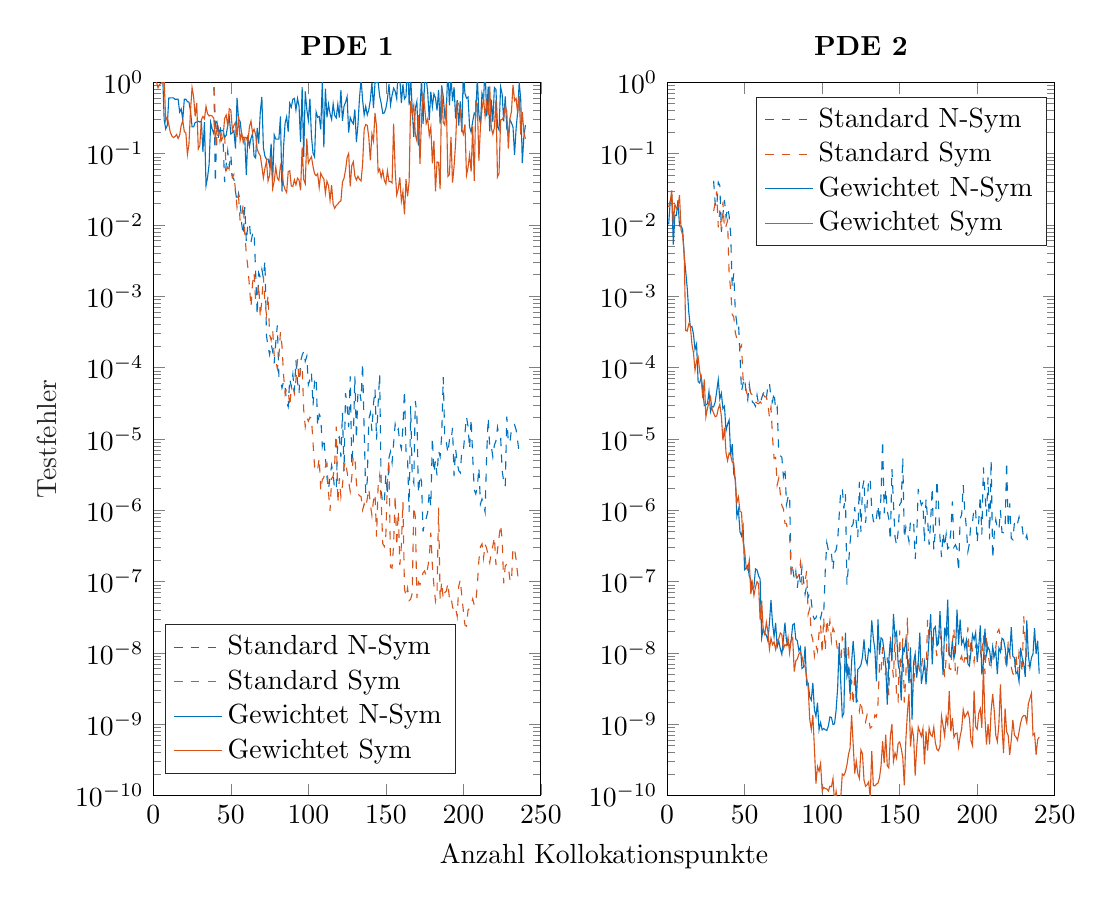
\begin{tikzpicture}

\begin{axis}[%
name = ax1,
width=1.938in,
height=3.566in,
at={(0.758in,0.481in)},
scale only axis,
xmin=0,
xmax=250,
%xlabel style={font=\color{white!15!black}},
%xlabel={amount of collocation points},
ymode=log,
ymin=1e-10,
ymax=1,
yminorticks=true,
ylabel style={font=\color{white!15!black}},
ylabel={Testfehler},
axis background/.style={fill=white},
title style={font=\bfseries},
title={\ac{PDE} 1},
legend style={legend cell align=left, align=left, draw=white!15!black},
legend pos = south west
]
\addplot [color=mycolor1, dashed]
  table[row sep=crcr]{%
37	0.998741611743565\\
38	1.56698113662613\\
39	1.42136798220903\\
40	0.0390994708809781\\
41	0.248340994602959\\
42	0.164178755435491\\
43	0.257088561832482\\
44	0.167554018875751\\
45	0.15029555458974\\
46	0.0398405178523725\\
47	0.0694103139259503\\
48	0.109226237003303\\
49	0.0660520350648076\\
50	0.0964940963117123\\
51	0.047066728058674\\
52	0.0436910549210606\\
53	0.0293446055808344\\
54	0.0211006316855517\\
55	0.0276976929175761\\
56	0.0211921990730971\\
57	0.0103875764832617\\
58	0.00722064148989227\\
59	0.0177039765776462\\
60	0.00575367368897617\\
61	0.0105342257537943\\
62	0.0107192608931312\\
63	0.00571232584370718\\
64	0.00747417551773089\\
65	0.00803971394621961\\
66	0.00217473435728519\\
67	0.000544432385404914\\
68	0.00212014655870951\\
69	0.00182510019522034\\
70	0.00238868533305021\\
71	0.0017977098497024\\
72	0.00313880426820937\\
73	0.00027769726807847\\
74	0.000199044228941125\\
75	0.000152182261049516\\
76	0.000213736913746099\\
77	0.000169367025339068\\
78	0.000114396474979274\\
79	0.000226111735248113\\
80	0.000391137412042775\\
81	7.48447510755534e-05\\
82	6.55505141003987e-05\\
83	5.16668725266678e-05\\
84	6.38462591333235e-05\\
85	5.29867437146364e-05\\
86	3.24099167953174e-05\\
87	2.8184817476018e-05\\
88	7.01514168349737e-05\\
89	5.38085245929132e-05\\
90	7.96424812544716e-05\\
91	4.61174110738538e-05\\
92	0.000125646798511569\\
93	6.3031063632174e-05\\
94	4.35928687395615e-05\\
95	0.000121609145040336\\
96	0.000148883059174348\\
97	0.000168190838442772\\
98	0.000122397013144537\\
99	0.00014420174279639\\
100	5.7515047468093e-05\\
101	6.76378663823085e-05\\
102	8.53128828505745e-05\\
103	2.88029952404401e-05\\
104	6.37022037984214e-05\\
105	7.3024085412654e-05\\
106	1.52023887962649e-05\\
107	2.20632120445652e-05\\
108	2.00185477740034e-05\\
109	7.88067193646658e-06\\
110	1.00867147672101e-05\\
111	5.48402793965064e-06\\
112	2.93095168890645e-06\\
113	1.95215757103906e-06\\
114	2.91291108089897e-06\\
115	4.23796744453142e-06\\
116	3.13522598038851e-06\\
117	1.92348417737964e-06\\
118	2.01161908124081e-06\\
119	1.02840686746486e-05\\
120	1.06591099515163e-05\\
121	5.55714251626593e-06\\
122	2.34661021522031e-05\\
123	3.52198276348803e-06\\
124	4.37132932321616e-05\\
125	2.90177717393938e-05\\
126	1.4652397314241e-05\\
127	7.53043162186121e-05\\
128	4.3100259585066e-06\\
129	9.69079551874086e-06\\
130	7.54924190527473e-05\\
131	9.94064516535165e-06\\
132	4.67727586663802e-05\\
133	4.79153665757931e-05\\
134	3.40215561696333e-05\\
135	0.000114985307212753\\
136	1.33877551191097e-05\\
137	1.7530018551204e-06\\
138	2.58690877819046e-06\\
139	1.89040058848899e-05\\
140	2.32115074470796e-05\\
141	1.28663555314656e-05\\
142	3.08685266256492e-05\\
143	4.97353206898588e-05\\
144	9.76269943031571e-06\\
145	3.06063970799495e-05\\
146	8.02500194259023e-05\\
147	1.86278142921825e-06\\
148	1.2262106793004e-06\\
149	1.29598968778843e-06\\
150	3.13788924793945e-06\\
151	1.61457367919837e-06\\
152	5.41168843918444e-06\\
153	6.61483082907421e-06\\
154	4.65463416295109e-06\\
155	8.66060960447168e-06\\
156	1.60554174002958e-05\\
157	1.25704435132296e-05\\
158	1.37370083810318e-05\\
159	8.79492131000692e-06\\
160	7.27568834029552e-06\\
161	1.46426066033323e-05\\
162	4.77355503902821e-05\\
163	6.71181707522991e-06\\
164	5.21785565158958e-06\\
165	9.46208204951476e-07\\
166	2.89965253619587e-05\\
167	2.88297546069058e-06\\
168	2.40391578823496e-06\\
169	3.41594613788299e-05\\
170	2.22097211157735e-05\\
171	1.71961815898652e-06\\
172	3.1020287614876e-06\\
173	2.5149947394526e-06\\
174	5.00024582034825e-07\\
175	6.87626018940762e-07\\
176	7.67321397865395e-07\\
177	9.4475997900953e-07\\
178	1.82680942861085e-06\\
179	1.13451757221411e-06\\
180	1.04683133181974e-05\\
181	3.37050654277901e-06\\
182	4.95802940869705e-06\\
183	3.07210305964395e-06\\
184	6.79044503370391e-06\\
185	5.64683856812964e-06\\
186	1.09663409100236e-05\\
187	7.30988803717691e-05\\
188	1.03728167460959e-05\\
189	9.06277390511079e-06\\
190	6.30410775187551e-06\\
191	9.66814870873023e-06\\
192	9.16927192839978e-06\\
193	1.42454825590166e-05\\
194	3.00812930895122e-06\\
195	7.16764222927213e-06\\
196	4.65214028225538e-06\\
197	3.59663400642876e-06\\
198	3.3488819956469e-06\\
199	6.98167184631782e-06\\
200	6.85437615960405e-06\\
201	1.20088282382427e-05\\
202	2.03161507994487e-05\\
203	1.50728294141533e-05\\
204	7.21549488818043e-06\\
205	1.92467401248508e-05\\
206	5.70364407070922e-06\\
207	1.93434035592951e-06\\
208	1.69378566581072e-06\\
209	2.12906590106934e-06\\
210	3.98689617203338e-06\\
211	1.21925504755968e-06\\
212	1.43524642520765e-06\\
213	1.20986212643129e-06\\
214	9.46273552959731e-07\\
215	5.85205886316498e-06\\
216	1.98246935840668e-05\\
217	7.53921539808911e-06\\
218	7.93029211895724e-06\\
219	5.60904436581328e-06\\
220	8.19994867790053e-06\\
221	9.3438873458862e-06\\
222	1.46148893186877e-05\\
223	1.11015863456521e-05\\
224	1.09517603379405e-05\\
225	3.60010360977298e-06\\
226	2.52063406169789e-06\\
227	2.13661485071182e-06\\
228	2.05038870653151e-05\\
229	8.74761571328583e-06\\
230	8.87575459032619e-06\\
231	1.34440711934136e-05\\
232	1.50879539022597e-05\\
233	1.58447361684466e-05\\
234	1.3385582362524e-05\\
235	9.32978721808128e-06\\
236	6.38942167646706e-06\\
};
\addlegendentry{Standard N-Sym}

\addplot [color=mycolor2, dashed]
  table[row sep=crcr]{%
37	1.03925796185995\\
38	1.21925853575973\\
39	0.953899537015336\\
40	0.311344674365069\\
41	0.132660921307261\\
42	0.217824106088015\\
43	0.147806099333084\\
44	0.190297468099253\\
45	0.170352138967985\\
46	0.182005937175475\\
47	0.0579651817610906\\
48	0.0648839471041575\\
49	0.0581654960960183\\
50	0.0617166726204858\\
51	0.0459164030685324\\
52	0.0507645101639707\\
53	0.0303631254070664\\
54	0.0177728361019\\
55	0.0246177936773342\\
56	0.0112600891781378\\
57	0.0128368554240275\\
58	0.0198812143769135\\
59	0.00759902417964253\\
60	0.00395308689811827\\
61	0.00252612426278695\\
62	0.00139783938225202\\
63	0.000703972076575243\\
64	0.00150950510885459\\
65	0.00212606095027751\\
66	0.000864330983407879\\
67	0.000971458217521648\\
68	0.00146520815743983\\
69	0.000503461636711222\\
70	0.0009021949542386\\
71	0.0019110610410173\\
72	0.000799707726148625\\
73	0.000555792506063182\\
74	0.00103842260381154\\
75	0.000289364693190282\\
76	0.000242065518552881\\
77	0.000333394065264891\\
78	0.000145603691467711\\
79	0.000125189409854398\\
80	9.61764715140256e-05\\
81	0.000141525100402107\\
82	0.000312655550304658\\
83	0.000200965990207046\\
84	7.94059253084178e-05\\
85	4.26646603217014e-05\\
86	5.07404198771821e-05\\
87	4.89951116840193e-05\\
88	2.80464863463559e-05\\
89	5.16817716176288e-05\\
90	5.31165012571666e-05\\
91	4.31421949008692e-05\\
92	6.73774851916858e-05\\
93	0.000130673279927884\\
94	6.47941950494557e-05\\
95	9.41970751252574e-05\\
96	0.00010536614127582\\
97	2.57175465160353e-05\\
98	1.47825057383311e-05\\
99	1.99510763194688e-05\\
100	1.76969983393116e-05\\
101	2.01210698749232e-05\\
102	1.95388984690625e-05\\
103	8.92735127536182e-06\\
104	4.09417429314551e-06\\
105	4.39064677881795e-06\\
106	3.72261747560998e-06\\
107	5.3722657377131e-06\\
108	1.88601698136726e-06\\
109	2.67873699710819e-06\\
110	2.88197576683857e-06\\
111	4.1220557150945e-06\\
112	4.53084972840134e-06\\
113	1.75858277789986e-06\\
114	9.80654038196249e-07\\
115	2.77021749078843e-06\\
116	3.00678087611361e-06\\
117	4.47092222649603e-06\\
118	1.4820455579212e-05\\
119	1.25768541336946e-06\\
120	2.8121578780349e-06\\
121	1.54376435834713e-06\\
122	2.22558315104981e-06\\
123	4.0402124734662e-06\\
124	4.83483574875709e-06\\
125	3.40876634286058e-06\\
126	2.51659107630697e-06\\
127	1.83311196433333e-06\\
128	2.87653275132804e-06\\
129	5.77164040881442e-06\\
130	5.67008450351805e-06\\
131	2.39642349841862e-06\\
132	1.71210266634858e-06\\
133	1.59223235113304e-06\\
134	1.5579776355551e-06\\
135	1.00630275626234e-06\\
136	1.22656372027186e-06\\
137	1.07475476244373e-06\\
138	1.45146144203689e-06\\
139	2.00664602291456e-06\\
140	1.20093984584332e-06\\
141	8.44387664886148e-07\\
142	1.37072368949775e-06\\
143	1.70316842126525e-06\\
144	4.26217667132134e-07\\
145	2.18666042084426e-06\\
146	3.09248034457976e-06\\
147	1.3225557835006e-06\\
148	3.39007867448254e-07\\
149	3.09588640279301e-07\\
150	4.54109492994959e-07\\
151	2.62528628401648e-06\\
152	5.15110685686548e-06\\
153	1.59515296416224e-07\\
154	1.54019627496282e-07\\
155	3.34701327889264e-07\\
156	1.6172625917632e-06\\
157	3.10186507146426e-07\\
158	9.76000212666445e-07\\
159	1.69670936078781e-07\\
160	3.1838807971335e-07\\
161	1.3142545842483e-06\\
162	7.92024072403252e-08\\
163	6.08781768780819e-08\\
164	8.08605520874472e-08\\
165	5.39873796293056e-08\\
166	5.64991390408776e-08\\
167	6.84055656008375e-08\\
168	1.12683275044212e-06\\
169	8.07399500146744e-07\\
170	5.87374219263026e-08\\
171	9.83787944441872e-08\\
172	9.04699001269549e-08\\
173	1.13158936838886e-07\\
174	1.32263112684328e-07\\
175	1.40683381305573e-07\\
176	1.18689939321293e-07\\
177	1.5662985753187e-07\\
178	2.17918422945607e-07\\
179	4.84386459997932e-07\\
180	1.64414559633563e-07\\
181	8.79592348262959e-08\\
182	5.32668583928808e-08\\
183	7.09421055650195e-08\\
184	1.08842901869188e-06\\
185	5.61670101331679e-08\\
186	9.90720011861956e-08\\
187	5.72096788657717e-08\\
188	6.97628354112689e-08\\
189	7.35082405153853e-08\\
190	9.52878394418211e-08\\
191	5.74430095018341e-08\\
192	6.13678932011308e-08\\
193	4.39093322222861e-08\\
194	3.86265774435235e-08\\
195	4.22445158160256e-08\\
196	3.23343047857472e-08\\
197	8.59866307982571e-08\\
198	1.05596978147715e-07\\
199	6.16113591742073e-08\\
200	3.85025325476407e-08\\
201	2.44913955123327e-08\\
202	2.36393051383788e-08\\
203	3.97154888108486e-08\\
204	4.21878035630763e-08\\
205	4.83791127575683e-08\\
206	5.72367898875326e-08\\
207	4.66266203112686e-08\\
208	5.13525010327476e-08\\
209	8.96788210705268e-08\\
210	1.98531108747124e-07\\
211	3.08130111870142e-07\\
212	3.37345463119476e-07\\
213	2.13114121586089e-07\\
214	3.32066082291138e-07\\
215	2.93284754371292e-07\\
216	2.2965533674757e-07\\
217	1.83629807169045e-07\\
218	2.58606539071948e-07\\
219	3.15453726279502e-07\\
220	4.18505087612653e-07\\
221	1.70786825372943e-07\\
222	2.75214854315864e-07\\
223	4.17517577011584e-07\\
224	6.24701936069449e-07\\
225	3.94944251897941e-07\\
226	9.44175825128013e-08\\
227	1.64728921725477e-07\\
228	1.7589382404759e-07\\
229	1.61073251210911e-07\\
230	1.07038829189054e-07\\
231	9.90944136747274e-08\\
232	2.99635917820618e-07\\
233	2.8564784231716e-07\\
234	2.03585285921126e-07\\
235	1.25163636986031e-07\\
236	9.63603937129132e-08\\
};
\addlegendentry{Standard Sym}

\addplot [color=mycolor1]
  table[row sep=crcr]{%
1	0.998741609443206\\
2	1.11782909710195\\
3	1.11926170760454\\
4	1.40983203621008\\
5	1.10969550695886\\
6	1.33567891758359\\
7	0.298996213312286\\
8	0.221313887435694\\
9	0.248421513930931\\
10	0.604876225289608\\
11	0.604876037814775\\
12	0.604875839547888\\
13	0.604858381653724\\
14	0.578491875925202\\
15	0.578481760326244\\
16	0.579452446988342\\
17	0.382238755805239\\
18	0.421590176235896\\
19	0.300165185534495\\
20	0.578508692946284\\
21	0.578469647977221\\
22	0.533563361892498\\
23	0.527798093185627\\
24	0.393450710515231\\
25	0.23642514478024\\
26	0.236770985306091\\
27	0.272801118053134\\
28	0.277764420011758\\
29	0.283422618535751\\
30	0.277373268400972\\
31	0.28355140962863\\
32	0.105560713632535\\
33	0.276111172374523\\
34	0.0354377115826865\\
35	0.0464653857366514\\
36	0.0707343866231824\\
37	0.27203081647291\\
38	0.219728424362293\\
39	0.190559915524707\\
40	0.264410299991884\\
41	0.281798643759454\\
42	0.203734690822977\\
43	0.203248608743901\\
44	0.211417677678289\\
45	0.210970597575964\\
46	0.171671991338889\\
47	0.179562595635948\\
48	0.251771985633483\\
49	0.324214718209404\\
50	0.18794129282178\\
51	0.19581643398208\\
52	0.209107387978555\\
53	0.117454597061782\\
54	0.604509872410409\\
55	0.301742279869405\\
56	0.283629555507286\\
57	0.182164411925352\\
58	0.168710088274823\\
59	0.161396700102654\\
60	0.0499953184063313\\
61	0.183367051426817\\
62	0.126367607131372\\
63	0.16382595726141\\
64	0.190177746239862\\
65	0.0920513416136276\\
66	0.086749673607173\\
67	0.228885726641179\\
68	0.138596460517003\\
69	0.383390652706299\\
70	0.623054832282331\\
71	0.122377297481263\\
72	0.0913981761595432\\
73	0.0833582776914546\\
74	0.0838178942191408\\
75	0.0678816544031598\\
76	0.137351260478364\\
77	0.0428950643459319\\
78	0.183157377819299\\
79	0.159715438941322\\
80	0.159178498286082\\
81	0.159640836741087\\
82	0.331176754767593\\
83	0.0294232107325849\\
84	0.122756855380896\\
85	0.266599583226172\\
86	0.328693572508701\\
87	0.203017733731328\\
88	0.508179187183779\\
89	0.44801036082651\\
90	0.57706184199745\\
91	0.594617979567265\\
92	0.408069524306715\\
93	0.59457479846108\\
94	0.46056590938674\\
95	0.144760557491992\\
96	0.852732788727093\\
97	0.0901285131939859\\
98	0.745554480530656\\
99	0.417643232811998\\
100	0.293971019079699\\
101	0.590843236027544\\
102	0.175364650322357\\
103	0.101807320849548\\
104	0.0900465105199209\\
105	0.384350346215022\\
106	0.322900282935706\\
107	0.331919475136758\\
108	0.218153713155314\\
109	1.00940892279894\\
110	0.121878293269635\\
111	0.814008297646505\\
112	0.322980718580268\\
113	0.491818564844289\\
114	0.362518162595553\\
115	0.300674398038549\\
116	0.498217539334676\\
117	0.342758279546107\\
118	0.316777508411193\\
119	0.488983970255965\\
120	0.319698057467612\\
121	0.772788244909034\\
122	0.287706422892413\\
123	0.459396966667727\\
124	0.525614775199957\\
125	0.626937965415375\\
126	0.197378050283326\\
127	0.32165588001073\\
128	0.283421553404393\\
129	0.261483038377733\\
130	0.416475506251789\\
131	0.14547737467135\\
132	0.255742221279286\\
133	0.606508982534549\\
134	1.10027664939163\\
135	0.564400806417723\\
136	0.348102395960063\\
137	0.457001345977805\\
138	0.348459051431221\\
139	0.412079014886288\\
140	0.565389524389465\\
141	0.989199984079448\\
142	0.435805764088374\\
143	0.989185137203699\\
144	0.998586253258111\\
145	0.998313509714498\\
146	0.638648220532664\\
147	0.504413413562605\\
148	0.366082519410418\\
149	0.372250813989348\\
150	0.432804902110466\\
151	0.576498573046489\\
152	0.944461702754474\\
153	0.48389708833378\\
154	0.655431625102434\\
155	0.825623143164555\\
156	0.747457498187471\\
157	0.585910145645681\\
158	1.66178433993654\\
159	1.13288880767446\\
160	0.511109874266554\\
161	0.936351716700421\\
162	0.584807011916181\\
163	0.633224231468053\\
164	2.3570619538081\\
165	0.476254971377984\\
166	1.16589988534355\\
167	0.415343223071657\\
168	0.172007983516451\\
169	0.429825539130111\\
170	0.538081343941462\\
171	0.129183779255546\\
172	0.407690022869368\\
173	1.10285089436092\\
174	0.260425841219897\\
175	1.0693544596134\\
176	1.14413713137681\\
177	0.717540814806354\\
178	0.294334205830768\\
179	0.738494706122012\\
180	0.452014418895125\\
181	0.688116647026599\\
182	0.60295376850186\\
183	0.403717870260455\\
184	0.782122735495744\\
185	0.261428633491739\\
186	0.9037747753403\\
187	0.629272294773887\\
188	0.337875198021642\\
189	0.401897294796143\\
190	1.58890049950707\\
191	0.473934705130939\\
192	1.19584551227356\\
193	0.545253385903161\\
194	0.850035308853414\\
195	0.309778590073588\\
196	0.562377838681034\\
197	0.246994752953103\\
198	0.539647446297994\\
199	0.200012462999764\\
200	1.48470154187804\\
201	0.69627394615953\\
202	0.597664524503675\\
203	0.620930879789426\\
204	0.237192192650629\\
205	0.199353298195462\\
206	0.282381708551619\\
207	0.37008383644784\\
208	0.342011756523453\\
209	1.17481258791866\\
210	0.351013910459668\\
211	0.261099473364089\\
212	0.700672823531981\\
213	0.570521157791295\\
214	1.63474634207842\\
215	0.333817112146321\\
216	0.870019926075269\\
217	0.205260110061192\\
218	0.568904894778107\\
219	0.279092775882512\\
220	0.843941397119131\\
221	0.793167933811759\\
222	0.236216745426569\\
223	0.214883456163585\\
224	0.861520932998331\\
225	0.681830333216637\\
226	0.282743984799185\\
227	0.635163927002778\\
228	0.224244188869927\\
229	0.186700138309314\\
230	0.298720114858592\\
231	0.269573685163897\\
232	0.236628090766631\\
233	0.0960263482240983\\
234	0.224829099264673\\
235	0.380839224431898\\
236	0.999888376319259\\
237	0.565859529695832\\
238	0.0738314169173088\\
239	0.170181029883029\\
240	0.249901487810149\\
};
\addlegendentry{Gewichtet N-Sym}

\addplot [color=mycolor2]
  table[row sep=crcr]{%
1	1.02484217867147\\
2	1.02554578477296\\
3	0.83635283475308\\
4	0.933329991098311\\
5	0.969606313860041\\
6	1.00547318953995\\
7	1.08072077358145\\
8	0.289742408891181\\
9	0.325262983759867\\
10	0.255326252458312\\
11	0.197858863131244\\
12	0.176554421267266\\
13	0.167846653057257\\
14	0.173316894260342\\
15	0.185073612685206\\
16	0.16296730150267\\
17	0.18155803742131\\
18	0.248244531043177\\
19	0.289567090018472\\
20	0.203197412317112\\
21	0.195063225333063\\
22	0.0972638751024082\\
23	0.136469593981298\\
24	0.403326081910369\\
25	0.842761947590126\\
26	0.625536036563596\\
27	0.333309067135447\\
28	0.511062828867\\
29	0.115888668665778\\
30	0.13040449228531\\
31	0.30002263029214\\
32	0.332287345854838\\
33	0.307815608439699\\
34	0.459295495125214\\
35	0.361490868064863\\
36	0.336765198402641\\
37	0.342548418816372\\
38	0.336596340436893\\
39	0.312626555955864\\
40	0.16357524095106\\
41	0.218479674444893\\
42	0.201835278109159\\
43	0.192118568464154\\
44	0.153855587238745\\
45	0.171794089622536\\
46	0.311875367378069\\
47	0.346751415391745\\
48	0.244875430289839\\
49	0.425235816276175\\
50	0.40883414024166\\
51	0.211234247648313\\
52	0.248889069690286\\
53	0.27276305420293\\
54	0.170704732836132\\
55	0.335933171190241\\
56	0.152404256606503\\
57	0.193825156714183\\
58	0.142849416988152\\
59	0.169683111158547\\
60	0.168013424225748\\
61	0.141697662968108\\
62	0.238040643064449\\
63	0.28520922204866\\
64	0.195638045323904\\
65	0.220286951422864\\
66	0.184416470372689\\
67	0.115755422903718\\
68	0.101707895679167\\
69	0.0932631506699045\\
70	0.0664120935883454\\
71	0.0455567768009428\\
72	0.0622742461464154\\
73	0.0778682497549726\\
74	0.041353463122343\\
75	0.049178997048163\\
76	0.0918031025351237\\
77	0.0324071907021634\\
78	0.0415618306515539\\
79	0.0641638278132399\\
80	0.0453540091467152\\
81	0.0421559818950792\\
82	0.0677443994633729\\
83	0.0569113666038654\\
84	0.0364683994499446\\
85	0.0313441585701817\\
86	0.0285700250686894\\
87	0.055672798295885\\
88	0.0574033670131144\\
89	0.0352216383191439\\
90	0.0345476682395708\\
91	0.0429122514392265\\
92	0.0364634822688497\\
93	0.0452570509449989\\
94	0.0424573776183379\\
95	0.0304817056595101\\
96	0.122482546721349\\
97	0.0433342168060967\\
98	0.0377987003407813\\
99	0.161713375708295\\
100	0.0733809934702112\\
101	0.0828172890494832\\
102	0.0902112258815324\\
103	0.0665102578248266\\
104	0.0523587596524288\\
105	0.0489596248693221\\
106	0.0521950279225069\\
107	0.0335577579103379\\
108	0.0531088349867518\\
109	0.047459828625217\\
110	0.0441312301521303\\
111	0.0279126869857855\\
112	0.0409372048311243\\
113	0.0354943593975902\\
114	0.0222140258203309\\
115	0.0362036111277441\\
116	0.0194146861168986\\
117	0.017100126277896\\
118	0.0186935999885637\\
119	0.0196328649477973\\
120	0.0210218450466058\\
121	0.0216479012769678\\
122	0.039813065178658\\
123	0.0449864125319129\\
124	0.059021442302048\\
125	0.0882925168638806\\
126	0.10051672267746\\
127	0.0347596885396955\\
128	0.0677105569186029\\
129	0.076882932177032\\
130	0.0484846731367857\\
131	0.0426999715074399\\
132	0.0480446752338148\\
133	0.0434754356950965\\
134	0.0413944900496132\\
135	0.0711869616731398\\
136	0.21899904400517\\
137	0.25658236837814\\
138	0.248363967607871\\
139	0.168664405592472\\
140	0.0802897736179331\\
141	0.188573824273064\\
142	0.150559688280388\\
143	0.370600363207112\\
144	0.240848992238541\\
145	0.0548591546546142\\
146	0.0605539017991303\\
147	0.0464054248781844\\
148	0.0577741017325724\\
149	0.0422330708889931\\
150	0.0375699887128825\\
151	0.0572519057604307\\
152	0.0406348192525929\\
153	0.0405749545869164\\
154	0.0387296904158216\\
155	0.261912353901395\\
156	0.0582992503556677\\
157	0.0263410722226635\\
158	0.0319647599912443\\
159	0.0464114013864724\\
160	0.0214391961265942\\
161	0.0291313738296188\\
162	0.0140454229187514\\
163	0.0436939043542569\\
164	0.0251281644203188\\
165	0.040396637919527\\
166	0.546918888399524\\
167	0.356148934684874\\
168	0.473713622217578\\
169	0.183712395704341\\
170	0.151354722070804\\
171	0.347255130464107\\
172	0.0718627018284358\\
173	0.320772036526761\\
174	0.715117905162348\\
175	0.450410046567719\\
176	0.263044037806802\\
177	0.307170952012439\\
178	0.178809092878458\\
179	0.235642460602787\\
180	0.0727370352628505\\
181	0.151905307483285\\
182	0.0296392799993229\\
183	0.0762257504382402\\
184	0.0753281317752419\\
185	0.0316454932428856\\
186	0.841235011140368\\
187	0.273152728376703\\
188	0.251140327465402\\
189	0.505342682776225\\
190	0.0478576734616419\\
191	0.0508786119231577\\
192	0.17150238807909\\
193	0.0391445173974968\\
194	0.0663909960610598\\
195	0.143021808020651\\
196	0.5197046690696\\
197	0.49929988855036\\
198	0.414645449425904\\
199	0.219226356527429\\
200	0.186878966904125\\
201	0.257129080820021\\
202	0.0495398501730366\\
203	0.0638479785782775\\
204	0.0959971625334947\\
205	0.0560245999955874\\
206	0.239888490774414\\
207	0.0414452911589673\\
208	0.540160980464651\\
209	0.494619130544883\\
210	0.078999229521905\\
211	0.239402038977085\\
212	0.416565538841353\\
213	0.597704345029667\\
214	0.332902699097246\\
215	0.507409910262476\\
216	0.349566300868792\\
217	0.871949422209032\\
218	0.229696746173245\\
219	0.18630735308048\\
220	0.231151902326783\\
221	0.571762879285483\\
222	0.0470321405061241\\
223	0.0530101846670843\\
224	0.296927190120473\\
225	0.298641880215295\\
226	0.328004628179816\\
227	0.461398090141728\\
228	0.389450120321725\\
229	0.117031657901161\\
230	0.30748111728075\\
231	0.387499311896518\\
232	0.918875315056545\\
233	0.551686924886223\\
234	0.592517683996341\\
235	0.367453146444282\\
236	0.640217039580792\\
237	0.185214663145421\\
238	0.384514337487475\\
239	0.198212448037092\\
240	0.161241036166096\\
};
\addlegendentry{Gewichtet Sym}

\end{axis}

\begin{axis}[%
name = ax2,
width=1.938in,
height=3.566in,
at={(3.327in,0.481in)},
scale only axis,
xmin=0,
xmax=250,
%xlabel style={font=\color{white!15!black}},
%xlabel={amount of collocation points},
ymode=log,
ymin=1e-10,
ymax=1,
yminorticks=true,
%ylabel style={font=\color{white!15!black}},
%ylabel={max. error in derivative/absolute},
axis background/.style={fill=white},
title style={font=\bfseries},
title={\ac{PDE} 2},
legend style={legend cell align=left, align=left, draw=white!15!black}
]
\addplot [color=mycolor1, dashed]
  table[row sep=crcr]{%
30	0.0413683547962787\\
31	0.0201309229210418\\
32	0.0173387844914555\\
33	0.0395787756842402\\
34	0.0356453728046247\\
35	0.00800006537221587\\
36	0.0139642878900886\\
37	0.0224332114669107\\
38	0.012768210151315\\
39	0.0175260420494299\\
40	0.013526401408511\\
41	0.00742158475420673\\
42	0.00132944746484476\\
43	0.00209224912073191\\
44	0.000608510676582019\\
45	0.000410702589317857\\
46	0.000446166480032262\\
47	0.000151230076015363\\
48	4.62171769545772e-05\\
49	5.99123736768903e-05\\
50	7.10912052557244e-05\\
51	4.19457530559386e-05\\
52	3.49557459004002e-05\\
53	5.78750765090064e-05\\
54	4.10165613006219e-05\\
55	3.2953989309914e-05\\
56	3.16211646141928e-05\\
57	2.86834822990079e-05\\
58	4.11635998241455e-05\\
59	3.01632882546699e-05\\
60	3.17229983759493e-05\\
61	3.72417327785257e-05\\
62	4.33236795104319e-05\\
63	4.5582757013829e-05\\
64	3.70098880115854e-05\\
65	5.49040899350262e-05\\
66	6.11957693634757e-05\\
67	3.68260598309078e-05\\
68	3.29221015797909e-05\\
69	4.53362513637146e-05\\
70	2.50386683805504e-05\\
71	2.7977328090012e-05\\
72	6.49077611625248e-06\\
73	5.7966956439337e-06\\
74	5.54233176941477e-06\\
75	2.97574442620352e-06\\
76	3.92862346476619e-06\\
77	1.19740306064875e-06\\
78	1.51867067155198e-06\\
79	1.65630231729885e-06\\
80	1.22303651206579e-07\\
81	1.52344315884623e-07\\
82	1.09741390363904e-07\\
83	1.39919371422437e-07\\
84	8.1750362312949e-08\\
85	1.31264101255191e-07\\
86	9.62060302533985e-08\\
87	1.59118578146877e-07\\
88	1.03191144407155e-07\\
89	6.65619265260986e-08\\
90	8.77762905415747e-08\\
91	6.02622033385458e-08\\
92	6.91719510004241e-08\\
93	5.3272975919505e-08\\
94	3.37597138022616e-08\\
95	2.95737731387247e-08\\
96	3.08734822984658e-08\\
97	3.65514146172252e-08\\
98	3.55638054005958e-08\\
99	3.0424685826258e-08\\
100	3.8786375555766e-08\\
101	3.49961731260784e-08\\
102	1.39460103798505e-07\\
103	3.49326872817191e-07\\
104	2.75366090374263e-07\\
105	2.91777857291953e-07\\
106	2.44694911083476e-07\\
107	1.46553530144811e-07\\
108	2.52783513648991e-07\\
109	2.77208248019439e-07\\
110	3.7506845499552e-07\\
111	8.48941008824156e-07\\
112	1.89958281079927e-06\\
113	2.03078517738153e-06\\
114	1.05089182250717e-06\\
115	1.68131418117751e-06\\
116	8.98113932112921e-08\\
117	1.72177622381753e-07\\
118	3.47486125956697e-07\\
119	5.87132948398628e-07\\
120	6.44287615675365e-07\\
121	1.10310747008548e-06\\
122	6.69722330301492e-07\\
123	4.21250394677664e-07\\
124	2.50122887537896e-06\\
125	4.95428284841282e-07\\
126	2.01485774761062e-06\\
127	2.66586153733865e-06\\
128	6.6659190367524e-07\\
129	1.16280023430317e-06\\
130	2.79960008597868e-06\\
131	2.64721623760567e-06\\
132	1.03310118764952e-06\\
133	7.15383779409384e-07\\
134	6.3168859788798e-07\\
135	7.75611845332813e-07\\
136	1.17393221682471e-06\\
137	6.81379554948874e-07\\
138	1.66774213424675e-06\\
139	9.50926871859381e-06\\
140	9.04145798064082e-07\\
141	1.98180252970748e-06\\
142	9.80338242528855e-07\\
143	7.52208177474956e-07\\
144	3.7684133020327e-07\\
145	3.77332204849756e-06\\
146	1.24986421773388e-06\\
147	4.22085908613479e-07\\
148	3.2299361407695e-07\\
149	4.92411967242812e-07\\
150	1.19523163091828e-06\\
151	1.2930705713815e-06\\
152	5.46818594965998e-06\\
153	4.05682650028716e-07\\
154	5.8218359434703e-07\\
155	4.84597500738371e-07\\
156	3.6434911765415e-07\\
157	7.17611741515856e-07\\
158	7.18566273649746e-07\\
159	7.0199348647243e-07\\
160	2.07084110193101e-07\\
161	4.37829989562155e-07\\
162	1.98168358507556e-06\\
163	1.45838114129493e-06\\
164	1.17957372397504e-06\\
165	1.28783011887901e-06\\
166	3.53323605706279e-07\\
167	1.44397530221774e-06\\
168	7.60603482988231e-07\\
169	3.26265837069517e-07\\
170	7.13114183759078e-07\\
171	2.07544511318658e-06\\
172	2.77754952759945e-07\\
173	5.15997218716868e-07\\
174	2.64960533051094e-06\\
175	1.27094548882378e-06\\
176	4.136145263069e-07\\
177	2.20222668934067e-07\\
178	4.83790398853046e-07\\
179	3.0893105490426e-07\\
180	4.62656784050441e-07\\
181	2.87895406958505e-07\\
182	3.06899948149253e-07\\
183	5.10733329562446e-07\\
184	1.32548418851908e-06\\
185	3.0279772722519e-07\\
186	3.27817612444381e-07\\
187	2.85735501578087e-07\\
188	1.38732117360013e-07\\
189	7.56151599334842e-07\\
190	8.77453333575362e-07\\
191	2.24928843542416e-06\\
192	9.61522294905953e-07\\
193	5.77750146807388e-07\\
194	2.62867325573346e-07\\
195	3.44961696652213e-07\\
196	6.97289823978209e-07\\
197	6.8693618626714e-07\\
198	1.08751907673676e-06\\
199	9.89652230831695e-07\\
200	3.57387610366855e-07\\
201	6.98350458655517e-07\\
202	1.59993155274263e-06\\
203	4.55398622034586e-07\\
204	3.9961573731484e-06\\
205	1.70615725289536e-06\\
206	8.21061887923413e-07\\
207	2.87846664570601e-06\\
208	3.90580536357987e-07\\
209	4.97430866727017e-06\\
210	2.08924917909428e-07\\
211	4.63653922117002e-07\\
212	7.34592507267706e-07\\
213	5.62241974311206e-07\\
214	5.23836331596528e-07\\
215	9.99196450607309e-07\\
216	4.89310584661506e-07\\
217	4.84144338147585e-07\\
218	5.50563742929278e-07\\
219	4.77977190312118e-06\\
220	5.61930428577551e-07\\
221	1.2469771477619e-06\\
222	4.03134647997128e-07\\
223	3.85013904424802e-07\\
224	6.57287410783802e-07\\
225	7.3831541011482e-07\\
226	6.47820382226882e-07\\
227	8.02694264272208e-07\\
228	6.1157477496826e-07\\
229	5.8285184945106e-07\\
230	3.96202177811548e-07\\
231	3.81017529527128e-07\\
232	4.46489492114677e-07\\
233	2.95233564663469e-07\\
};
\addlegendentry{Standard N-Sym}

\addplot [color=mycolor2, dashed]
  table[row sep=crcr]{%
30	0.0156165029602802\\
31	0.0206211465072624\\
32	0.0295584964080999\\
33	0.00927803461041649\\
34	0.0159249976301867\\
35	0.00862335182643981\\
36	0.020984517083313\\
37	0.00871507282010392\\
38	0.00962086651639371\\
39	0.0115010684216514\\
40	0.00207464330283857\\
41	0.00122030004488424\\
42	0.000556530342384121\\
43	0.000510003733881215\\
44	0.000307882634830892\\
45	0.000251860991684782\\
46	0.000235774010807543\\
47	0.000186330301295001\\
48	0.000204969983493675\\
49	6.8099142323863e-05\\
50	6.44734682604398e-05\\
51	4.73624869364031e-05\\
52	3.98578620762757e-05\\
53	5.26083092984297e-05\\
54	4.35274863936908e-05\\
55	4.11066849581587e-05\\
56	3.36175649056081e-05\\
57	3.28503579053452e-05\\
58	3.17145818427012e-05\\
59	3.10498011538152e-05\\
60	3.30183523965522e-05\\
61	3.1219647015579e-05\\
62	4.18783949992507e-05\\
63	3.88818569205807e-05\\
64	3.86200270285908e-05\\
65	3.143037612513e-05\\
66	2.01012365858844e-05\\
67	2.78648830850936e-05\\
68	1.05245356387118e-05\\
69	5.30024177347599e-06\\
70	5.48944174028065e-06\\
71	2.25847255264089e-06\\
72	2.80170159194792e-06\\
73	1.70781589778346e-06\\
74	1.16560023771806e-06\\
75	1.05259159882687e-06\\
76	6.58804020003956e-07\\
77	6.43812172351765e-07\\
78	4.88214001337361e-07\\
79	4.39231584270505e-07\\
80	1.38308874131354e-07\\
81	1.6308902417439e-07\\
82	1.41344560056211e-07\\
83	1.24344060908887e-07\\
84	1.13762238518333e-07\\
85	1.24225435382819e-07\\
86	1.82922842872912e-07\\
87	9.20334242149323e-08\\
88	8.81792232565459e-08\\
89	9.85131437258868e-08\\
90	1.40817532856552e-07\\
91	3.48437512731614e-08\\
92	4.2045629894405e-08\\
93	1.84537453096212e-08\\
94	1.50541453747266e-08\\
95	9.05707531195787e-09\\
96	1.27527828297502e-08\\
97	1.05814147999261e-08\\
98	1.91062720089619e-08\\
99	2.49200663438032e-08\\
100	9.65593449642199e-09\\
101	3.14235968912335e-08\\
102	1.08207566240637e-08\\
103	2.93821680319439e-08\\
104	1.9138684304032e-08\\
105	2.80289653153964e-08\\
106	1.48378787589998e-08\\
107	2.209395699726e-08\\
108	1.9473130052905e-08\\
109	1.52746603143683e-08\\
110	1.03703601261884e-08\\
111	1.21248149298481e-08\\
112	5.93253479674871e-09\\
113	1.69703354702122e-08\\
114	1.2218128508934e-08\\
115	5.90233496799986e-09\\
116	4.64660993015897e-09\\
117	1.30560163791316e-08\\
118	2.14252415808858e-09\\
119	4.1832530772723e-09\\
120	1.8452669392488e-09\\
121	5.21116905183305e-09\\
122	2.34879815597111e-09\\
123	2.07361516846305e-09\\
124	1.52696544297726e-09\\
125	2.13252704384104e-09\\
126	1.46235645814841e-09\\
127	1.24446336569051e-09\\
128	1.07004360927476e-09\\
129	1.36415634344189e-09\\
130	1.18959320172252e-09\\
131	8.77002193089282e-10\\
132	9.2178131794185e-10\\
133	9.95769244838129e-10\\
134	1.34052235978288e-09\\
135	1.27187810283758e-09\\
136	1.90702320601588e-09\\
137	6.93977530996648e-09\\
138	5.50668144416733e-09\\
139	1.19801806808262e-08\\
140	5.24254673006652e-09\\
141	4.94421176222559e-09\\
142	8.64618576734699e-09\\
143	2.54305987379411e-09\\
144	1.71206583354788e-08\\
145	7.3311672288412e-09\\
146	4.51001647139293e-09\\
147	1.75037233596242e-08\\
148	2.20668394668166e-09\\
149	2.07584316402887e-09\\
150	2.06664925173072e-08\\
151	3.46006656659625e-09\\
152	1.59292613544082e-08\\
153	1.99932365108069e-09\\
154	4.78215239629876e-09\\
155	3.11713448386541e-08\\
156	4.14124967998419e-09\\
157	4.19048906685759e-09\\
158	2.63767546346272e-09\\
159	3.17595399978998e-09\\
160	8.76135228256025e-09\\
161	4.4645243058028e-09\\
162	7.91283521345276e-09\\
163	5.23254178874666e-09\\
164	5.85795212337814e-09\\
165	9.27184029553274e-09\\
166	7.23141480030165e-09\\
167	4.62273397339175e-09\\
168	2.90328923679972e-08\\
169	1.54229821136553e-08\\
170	1.75970673033099e-08\\
171	1.68330199709632e-08\\
172	1.27848084341409e-08\\
173	1.33223057030563e-08\\
174	8.98109175917483e-09\\
175	2.0675334222453e-08\\
176	1.85713011635613e-08\\
177	9.7481717697967e-09\\
178	1.17393635923335e-08\\
179	4.57448545709838e-09\\
180	8.39176897415861e-09\\
181	3.27818904799493e-08\\
182	6.01802081084957e-09\\
183	5.86918313949525e-09\\
184	1.40532002701477e-08\\
185	2.22054581389131e-08\\
186	4.61576543653308e-09\\
187	5.0457886202615e-09\\
188	7.92358476053856e-09\\
189	7.98874949525796e-09\\
190	9.02715913131402e-09\\
191	6.60746551917057e-09\\
192	8.53460357941316e-09\\
193	8.2765463926826e-09\\
194	2.29076076441181e-08\\
195	7.59480411893776e-09\\
196	1.57025447089509e-08\\
197	1.06229506302569e-08\\
198	7.40581640457094e-09\\
199	1.2836032625696e-08\\
200	1.29194918097042e-08\\
201	9.66188179463146e-09\\
202	1.05195308020001e-08\\
203	8.11070677286807e-09\\
204	1.7855676381906e-08\\
205	5.04791591859899e-09\\
206	1.74208233394424e-08\\
207	9.83948522659261e-09\\
208	6.80532619146135e-09\\
209	6.4128712895517e-09\\
210	7.15637454851148e-09\\
211	1.28689185974196e-08\\
212	1.16831541663309e-08\\
213	1.93386412439267e-08\\
214	2.13485010780445e-08\\
215	1.68859400377294e-08\\
216	1.03173221077668e-08\\
217	1.03637287085512e-08\\
218	8.56964960105344e-09\\
219	5.81974612945402e-09\\
220	1.43360375237656e-08\\
221	9.52086554040221e-09\\
222	6.25684015709282e-09\\
223	5.09795716752137e-09\\
224	4.89614682130934e-09\\
225	9.71638441926714e-09\\
226	4.99961261279935e-09\\
227	1.02830676161625e-08\\
228	8.85902714381492e-09\\
229	5.30143794141846e-09\\
230	3.24833535625402e-08\\
231	1.49796937076729e-08\\
232	8.35570990176393e-09\\
233	6.45705033885946e-09\\
};
\addlegendentry{Standard Sym}

\addplot [color=mycolor1]
  table[row sep=crcr]{%
1	0.0101596215796438\\
2	0.0209537371572384\\
3	0.0245390735516798\\
4	0.00528098624824838\\
5	0.0136741883093289\\
6	0.0135500484337859\\
7	0.0222106118420004\\
8	0.00961367599176388\\
9	0.0096637580436208\\
10	0.00866125047112387\\
11	0.003840004227189\\
12	0.00222573399720299\\
13	0.00128159662985117\\
14	0.000591104912869567\\
15	0.000367649770062095\\
16	0.000377347843405429\\
17	0.000294245868401322\\
18	0.000179432585067807\\
19	0.000213432657603707\\
20	6.34830374971473e-05\\
21	6.07325403002568e-05\\
22	7.43595620806836e-05\\
23	4.90886517223177e-05\\
24	2.91848275730811e-05\\
25	2.99194429996819e-05\\
26	3.10288895838673e-05\\
27	4.59597833706304e-05\\
28	2.40615207250938e-05\\
29	2.84311590011965e-05\\
30	2.80912545879142e-05\\
31	3.29113727378649e-05\\
32	4.65933409922181e-05\\
33	6.76565891261638e-05\\
34	3.62153232478235e-05\\
35	4.35919016870123e-05\\
36	2.64843513462232e-05\\
37	2.87920345032333e-05\\
38	1.30001618462994e-05\\
39	1.60775955551917e-05\\
40	1.83882034626159e-05\\
41	5.78145694063448e-06\\
42	8.44126712210014e-06\\
43	3.23476890640162e-06\\
44	2.72669542400461e-06\\
45	8.24026793910804e-07\\
46	1.02232345128295e-06\\
47	4.97338443872231e-07\\
48	4.34742008836864e-07\\
49	5.83261561271087e-07\\
50	1.46374830201079e-07\\
51	1.54521306972022e-07\\
52	1.68216994139714e-07\\
53	1.19475503879141e-07\\
54	1.05526201471529e-07\\
55	7.8578450413147e-08\\
56	8.35269426957552e-08\\
57	1.50448982605411e-07\\
58	1.45115028660214e-07\\
59	1.20497461897351e-07\\
60	1.08319795577572e-07\\
61	1.63353324755811e-08\\
62	2.16279849307721e-08\\
63	1.86592136186547e-08\\
64	1.77202769124918e-08\\
65	1.4708367856997e-08\\
66	2.62438918374741e-08\\
67	5.49131228821942e-08\\
68	2.57481678200833e-08\\
69	1.69418162276891e-08\\
70	2.62605734380195e-08\\
71	1.21578780376552e-08\\
72	1.4728779751394e-08\\
73	1.14047801202943e-08\\
74	9.49178802223116e-09\\
75	1.53294129612291e-08\\
76	2.64162369201237e-08\\
77	1.46629745012561e-08\\
78	1.2632498935794e-08\\
79	1.26535593114596e-08\\
80	1.48044654313395e-08\\
81	2.46135322123919e-08\\
82	2.56605684478828e-08\\
83	1.56148785013244e-08\\
84	1.47198177535834e-08\\
85	1.07111407521288e-08\\
86	1.20046703688814e-08\\
87	6.04191358055672e-09\\
88	6.30490387676375e-09\\
89	1.23017392938962e-08\\
90	3.56237928045289e-09\\
91	3.73277350695922e-09\\
92	2.41558550939658e-09\\
93	2.17181317374582e-09\\
94	3.79505293857108e-09\\
95	1.58671276118127e-09\\
96	1.29012595051492e-09\\
97	2.00361471858201e-09\\
98	8.32093727254346e-10\\
99	1.04809538825634e-09\\
100	8.31214985730355e-10\\
101	8.68115468399822e-10\\
102	8.3462453615013e-10\\
103	8.15273959453577e-10\\
104	9.41476507865247e-10\\
105	1.26272847733588e-09\\
106	1.24136501078453e-09\\
107	9.89007264973196e-10\\
108	1.01250552386745e-09\\
109	1.57072888029575e-09\\
110	3.23399645951739e-09\\
111	1.38299350860294e-08\\
112	3.84645221229718e-09\\
113	1.2736757204479e-09\\
114	1.43777101335729e-09\\
115	1.91577712582713e-08\\
116	4.68491034855134e-09\\
117	5.87329573864537e-09\\
118	2.6587743118256e-09\\
119	7.39945660299668e-09\\
120	1.47005823070145e-08\\
121	7.41064054565754e-09\\
122	1.99818694923692e-09\\
123	5.86187065554356e-09\\
124	6.16164352873483e-09\\
125	6.76244216180066e-09\\
126	8.75257422094933e-09\\
127	1.54312880251695e-08\\
128	8.17695611221581e-09\\
129	6.96769897334804e-09\\
130	1.12116872452717e-08\\
131	1.0313789933214e-08\\
132	2.85093902929745e-08\\
133	1.6133727687162e-08\\
134	1.12253466522105e-08\\
135	3.99758059987931e-09\\
136	2.94491157015742e-08\\
137	9.44639932942692e-09\\
138	1.62251923008228e-08\\
139	1.53501678035184e-08\\
140	1.02044820371461e-08\\
141	6.60075027969498e-09\\
142	1.88606052997642e-09\\
143	7.92003362892757e-09\\
144	1.4755306199099e-08\\
145	7.87729925733061e-09\\
146	3.50979688645836e-08\\
147	1.7187151923892e-08\\
148	1.95894208632197e-08\\
149	7.07990677195625e-09\\
150	5.6201634457409e-09\\
151	2.15927820068629e-09\\
152	1.1498146101907e-08\\
153	1.05895601176798e-08\\
154	1.54187246304005e-08\\
155	8.40628122666942e-09\\
156	3.76922570932692e-09\\
157	1.19116481123172e-08\\
158	1.15489195984253e-09\\
159	7.33591665191824e-09\\
160	9.70036351244374e-09\\
161	4.51423187719513e-09\\
162	7.63298424466541e-09\\
163	1.92309890234554e-08\\
164	3.67980879101282e-09\\
165	5.1691970703871e-09\\
166	7.31903382344967e-09\\
167	3.6038716455522e-09\\
168	7.47819217661316e-09\\
169	1.69693622487088e-08\\
170	3.47468806505269e-08\\
171	6.8767249672419e-09\\
172	2.17038818028925e-08\\
173	2.32236192498902e-08\\
174	1.27125082682866e-08\\
175	1.35066189899113e-08\\
176	3.84007661224928e-08\\
177	1.37145865775068e-08\\
178	4.86232787366703e-09\\
179	2.26019244431441e-08\\
180	1.68054437033049e-08\\
181	5.5860576830824e-08\\
182	9.21486964511331e-09\\
183	8.75492439655901e-09\\
184	1.46109289111962e-08\\
185	8.32939595074578e-09\\
186	1.04450007532009e-08\\
187	4.03242004232141e-08\\
188	1.30776373064023e-08\\
189	2.93342693469256e-08\\
190	1.34555688813265e-08\\
191	1.55456642003671e-08\\
192	1.16666963867473e-08\\
193	1.50485920391574e-08\\
194	7.01373747968859e-09\\
195	6.54364817886943e-09\\
196	1.05427386820622e-08\\
197	1.80286953144204e-08\\
198	1.52210868353819e-08\\
199	1.92168998491837e-08\\
200	7.44836148314221e-09\\
201	1.20738099518292e-08\\
202	2.43200045657588e-08\\
203	4.94483065605067e-09\\
204	7.07197667093595e-09\\
205	2.17838742599952e-08\\
206	9.48529399469322e-09\\
207	1.1949964850988e-08\\
208	1.08465044723616e-08\\
209	7.11922865104242e-09\\
210	1.22230230381604e-08\\
211	8.92297524757169e-09\\
212	1.05452243603921e-08\\
213	5.03159969245104e-09\\
214	1.16592702159579e-08\\
215	1.02895751918908e-08\\
216	1.59901130114548e-08\\
217	1.53409686065586e-08\\
218	1.17614207262307e-08\\
219	7.27581928039456e-09\\
220	1.15662291966245e-08\\
221	9.86651360612711e-09\\
222	2.2838266389158e-08\\
223	8.88088291794986e-09\\
224	8.57914417284888e-09\\
225	5.15424480873605e-09\\
226	5.40922456826465e-09\\
227	3.96399124635849e-09\\
228	1.17720685421929e-08\\
229	8.5068152522183e-09\\
230	7.10630942979407e-09\\
231	4.60144294889275e-09\\
232	2.83929036948294e-08\\
233	9.09074071575589e-09\\
234	6.17623707732662e-09\\
235	8.56192938769595e-09\\
236	9.66995350459854e-09\\
237	2.2238271557562e-08\\
238	9.61854318415334e-09\\
239	1.48541873246089e-08\\
240	5.12103814909182e-09\\
};
\addlegendentry{Gewichtet N-Sym}

\addplot [color=mycolor2]
  table[row sep=crcr]{%
1	0.017850133296025\\
2	0.0215223323179307\\
3	0.0303694794898038\\
4	0.0101546936893073\\
5	0.0193027140968857\\
6	0.0171716965278758\\
7	0.0177455451436723\\
8	0.0260478628785181\\
9	0.00858505063369513\\
10	0.0072328358773518\\
11	0.00400244825112733\\
12	0.000331295959528854\\
13	0.000324864094596089\\
14	0.000411132016005344\\
15	0.000387394081649617\\
16	0.000212453362236742\\
17	0.000161550747999173\\
18	9.15387418167768e-05\\
19	0.000124279127199367\\
20	0.000140363508541297\\
21	8.93705994624572e-05\\
22	6.91547070654774e-05\\
23	3.71933318298046e-05\\
24	6.81622593099451e-05\\
25	2.04037883357322e-05\\
26	2.66153590159635e-05\\
27	3.2600545204875e-05\\
28	3.8501507708899e-05\\
29	2.6019099523017e-05\\
30	2.29843992971546e-05\\
31	2.04199193976073e-05\\
32	2.09939771936285e-05\\
33	2.64231045568053e-05\\
34	3.03895085880246e-05\\
35	2.07527504145211e-05\\
36	9.53868577024952e-06\\
37	1.43350198354986e-05\\
38	6.37499047473344e-06\\
39	4.95348306775445e-06\\
40	6.33687855977616e-06\\
41	5.87589651757092e-06\\
42	4.71811970248481e-06\\
43	4.5809647938877e-06\\
44	2.54904929131161e-06\\
45	1.28115088082748e-06\\
46	1.53156229398821e-06\\
47	9.613220529614e-07\\
48	9.34982911982019e-07\\
49	3.59418602102757e-07\\
50	2.71387171346671e-07\\
51	1.55529854745096e-07\\
52	1.4522872268663e-07\\
53	1.97434136317565e-07\\
54	6.66604374477409e-08\\
55	9.52412998467267e-08\\
56	6.38340873493348e-08\\
57	8.28485808845869e-08\\
58	9.96779980777518e-08\\
59	9.26460853034605e-08\\
60	2.8940217722262e-08\\
61	5.37132668898543e-08\\
62	2.01576535463488e-08\\
63	1.80167242236351e-08\\
64	2.6784596318663e-08\\
65	1.9885395774466e-08\\
66	1.12653613104641e-08\\
67	1.6033213423583e-08\\
68	1.301488217198e-08\\
69	1.41914411333488e-08\\
70	1.12159702636561e-08\\
71	1.49256647041796e-08\\
72	1.58232711378048e-08\\
73	1.89616078394295e-08\\
74	1.80717685815956e-08\\
75	1.13574162852181e-08\\
76	1.30239591888959e-08\\
77	1.26260002453193e-08\\
78	1.64197581087322e-08\\
79	9.94380588981159e-09\\
80	1.49425490869604e-08\\
81	1.62526150315756e-08\\
82	5.44465617036138e-09\\
83	7.68231833703226e-09\\
84	8.18261169932555e-09\\
85	9.62904161960765e-09\\
86	1.02589779449325e-08\\
87	8.88971313228737e-09\\
88	6.85736362138201e-09\\
89	6.43195979810329e-09\\
90	4.52970344566594e-09\\
91	3.2524707371806e-09\\
92	1.17266202304123e-09\\
93	8.41791858441354e-10\\
94	1.34439681609422e-09\\
95	4.70819216946694e-10\\
96	1.46829048919273e-10\\
97	2.5354085497753e-10\\
98	2.18453366507276e-10\\
99	2.8199892421199e-10\\
100	1.1710626912631e-10\\
101	1.29658284109269e-10\\
102	1.25304822073957e-10\\
103	1.23879573266095e-10\\
104	1.15286724611252e-10\\
105	1.34858235689705e-10\\
106	1.3264656040235e-10\\
107	1.73306646811255e-10\\
108	7.79642461701258e-11\\
109	1.14475151580251e-10\\
110	7.71593344772725e-11\\
111	8.18297651861144e-11\\
112	9.40101330115795e-11\\
113	2.00411132134093e-10\\
114	1.90272908540123e-10\\
115	2.13136619464649e-10\\
116	2.68410849102452e-10\\
117	3.75978692623846e-10\\
118	4.60473548180573e-10\\
119	1.34200528467687e-09\\
120	5.33545874148444e-10\\
121	2.03164096657105e-10\\
122	3.02070757296491e-10\\
123	2.03793371067462e-10\\
124	1.74373182559862e-10\\
125	4.35209757121413e-10\\
126	3.86151000064672e-10\\
127	1.63999924751579e-10\\
128	1.34284694475184e-10\\
129	1.40925271452375e-10\\
130	1.547043604333e-10\\
131	9.41851874269872e-11\\
132	4.18811985092304e-10\\
133	1.37283795442755e-10\\
134	1.36337940936926e-10\\
135	1.44496303811081e-10\\
136	1.48995094040316e-10\\
137	1.77234615872379e-10\\
138	2.62303789799745e-10\\
139	5.75326453144953e-10\\
140	2.8621527370376e-10\\
141	7.11981362755409e-10\\
142	2.60473476121348e-10\\
143	2.4386520580677e-10\\
144	6.80590250823343e-10\\
145	1.00387642643085e-09\\
146	3.0019248198343e-10\\
147	3.94588028918008e-10\\
148	3.33795879825516e-10\\
149	5.35317123961931e-10\\
150	5.63289304089665e-10\\
151	4.60414817382571e-10\\
152	3.40009631560889e-10\\
153	1.38750955169797e-10\\
154	6.1185545519038e-10\\
155	1.45101153314897e-09\\
156	2.66156940931239e-09\\
157	4.8528725482555e-10\\
158	8.80921946500024e-10\\
159	6.70453137452398e-10\\
160	1.90358062646112e-10\\
161	4.77027195522339e-10\\
162	9.09710418106613e-10\\
163	7.7815343058063e-10\\
164	6.73451960864213e-10\\
165	8.66926863629658e-10\\
166	2.73327915856214e-10\\
167	7.93003773758016e-10\\
168	4.25759871802711e-10\\
169	8.81762218796212e-10\\
170	7.1136418977602e-10\\
171	6.72580990901395e-10\\
172	9.03169761201639e-10\\
173	5.51602485909797e-10\\
174	4.46810477505721e-10\\
175	4.24430601775327e-10\\
176	4.89611018394953e-10\\
177	1.28989746661645e-09\\
178	9.51370870971857e-10\\
179	6.8572980627124e-10\\
180	1.27168353625251e-09\\
181	9.93788273895291e-10\\
182	2.90822688153725e-09\\
183	7.94325161201925e-10\\
184	1.21063287172873e-09\\
185	6.54321929971502e-10\\
186	7.39135530558599e-10\\
187	7.50022266515771e-10\\
188	4.78879269572019e-10\\
189	6.72079503161171e-10\\
190	8.65236327030061e-10\\
191	1.59837609814417e-09\\
192	1.24270371770763e-09\\
193	1.3694904099637e-09\\
194	1.49806372862216e-09\\
195	1.21305732125876e-09\\
196	5.8833693472593e-10\\
197	4.99647767604472e-10\\
198	2.94092861174988e-09\\
199	9.22474208131518e-10\\
200	8.49732062491171e-10\\
201	1.41294065336695e-09\\
202	1.64889546461211e-09\\
203	8.86902440377924e-10\\
204	6.38616770576306e-09\\
205	1.2499159485202e-09\\
206	5.16688691831746e-10\\
207	9.96957738585991e-10\\
208	5.1968296332916e-10\\
209	1.54908452731917e-09\\
210	2.63259136712435e-09\\
211	1.54582247002821e-09\\
212	6.98992308478807e-10\\
213	5.6980747897839e-10\\
214	9.96652316231916e-10\\
215	3.60277840893986e-09\\
216	9.26725696182018e-10\\
217	3.94403176784408e-10\\
218	1.66731550788057e-09\\
219	7.84199372105832e-10\\
220	6.93662904893699e-10\\
221	3.72658293112949e-10\\
222	6.02967231699836e-10\\
223	1.14838094589231e-09\\
224	7.03300195858958e-10\\
225	6.59974519479078e-10\\
226	5.9558791232206e-10\\
227	7.80440156944451e-10\\
228	1.03746033985885e-09\\
229	1.24600063600155e-09\\
230	1.32395672203245e-09\\
231	1.31378619094846e-09\\
232	1.04871750172819e-09\\
233	1.94305782574844e-09\\
234	2.27874141778273e-09\\
235	2.72358469111111e-09\\
236	7.04711844434769e-10\\
237	7.43603845165808e-10\\
238	3.7309388911666e-10\\
239	6.05891781191303e-10\\
240	6.60266397112252e-10\\
};
\addlegendentry{Gewichtet Sym}

\end{axis}
\path (ax1.south east) -- (ax2.south west)
  node[midway,below=5mm] {Anzahl Kollokationspunkte};
\end{tikzpicture}%
}
\caption{Testfehler beim Greedy-Verfahren}
\label{fig:error-greedy}
\end{figure}

Wir erkennen, dass für die erste \ac{PDE} nur die Standardverfahren vernünftige Ergebnisse liefern. Diese pendeln sich nach ungefähr $110$ Kollokationspunkten für das nicht-symmetrische Verfahren bei einem Testfehler von rund $10^{-5}$ und nach ungefähr $160$ Iterationen für das symmetrische bei einem Testfehler von rund $10^{-7}$ ein. Damit benötigt die Greedy-Punktwahl jeweils $80$ beziehungsweise $320$ Kollokationspunkte weniger, um das gleiche Ergebnis wie die Gitterpunktwahl zu erzielen.

Die gewichteten Verfahren hingegen geben uns beide keine vernünftigen Ergebnisse. Ein Grund dafür wird erkennbar, wenn man sich anschaut, wo die Kollokationspunkte hingelegt werden. Dies ist in Abbildung \ref{fig:greedy-points} dargestellt.
\begin{figure}[ht]
\centering
\resizebox {\columnwidth} {!} {
% This file was created by matlab2tikz.
%
%The latest updates can be retrieved from
%  http://www.mathworks.com/matlabcentral/fileexchange/22022-matlab2tikz-matlab2tikz
%where you can also make suggestions and rate matlab2tikz.
%
%
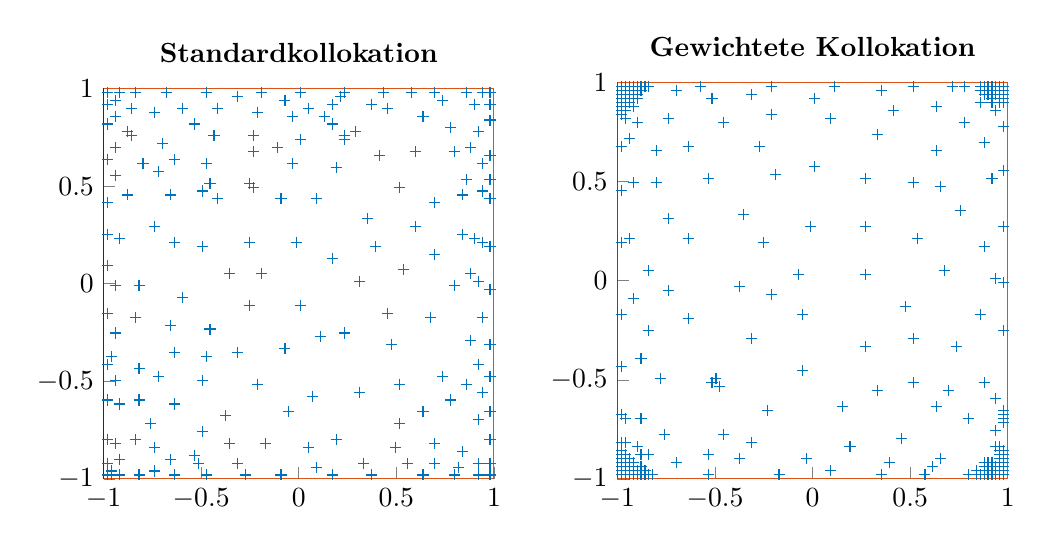
\begin{tikzpicture}

\begin{axis}[%
width=1.952in,
%height=3.566in,
height=1.952in,
at={(0.758in,0.481in)},
scale only axis,
xmin=-1,
xmax=1,
%ymin=-1.82648556876061,
%ymax=1.82648556876061,
ymin=-1,
ymax=1,
axis background/.style={fill=white},
title style={font=\bfseries},
title={Standardkollokation},
axis x line*=bottom,
axis y line*=left,
legend style={legend cell align=left, align=left, draw=white!15!black}
]
\addplot [color=mycolor1, draw=none, mark=+, mark options={solid, mycolor1}]
  table[row sep=crcr]{%
-0.494949494949495	-0.494949494949495\\
0.515151515151515	0.494949494949495\\
0.515151515151515	-0.515151515151515\\
-0.494949494949495	0.474747474747475\\
-0.696969696969697	0.717171717171717\\
0.434343434343434	0.97979797979798\\
0.97979797979798	0.434343434343434\\
-0.252525252525252	-0.111111111111111\\
0.232323232323232	-0.252525252525252\\
0.0909090909090908	0.434343434343434\\
-0.474747474747475	0.97979797979798\\
-0.97979797979798	0.414141414141414\\
0.535353535353535	0.0707070707070707\\
-0.818181818181818	-0.0101010101010101\\
-0.757575757575758	-0.717171717171717\\
0.696969696969697	-0.818181818181818\\
0.878787878787879	-0.292929292929293\\
-0.171717171717172	-0.818181818181818\\
0.777777777777778	0.797979797979798\\
-0.252525252525252	0.212121212121212\\
-0.111111111111111	0.696969696969697\\
-0.474747474747475	-0.97979797979798\\
0.838383838383838	0.252525252525253\\
0.0707070707070707	-0.575757575757576\\
0.97979797979798	-0.474747474747475\\
0.292929292929293	0.777777777777778\\
-0.737373737373737	0.292929292929293\\
-0.97979797979798	-0.414141414141414\\
0.0101010101010102	0.97979797979798\\
0.191919191919192	-0.797979797979798\\
0.373737373737374	-0.97979797979798\\
0.97979797979798	-0.797979797979798\\
-0.97979797979798	-0.797979797979798\\
0.858585858585859	0.97979797979798\\
-0.97979797979798	0.818181818181818\\
-0.818181818181818	-0.434343434343434\\
0.171717171717172	0.131313131313131\\
0.97979797979798	-0.0303030303030303\\
-0.97979797979798	-0.97979797979798\\
0.97979797979798	0.97979797979798\\
-0.0909090909090909	-0.97979797979798\\
-0.818181818181818	-0.97979797979798\\
0.797979797979798	-0.97979797979798\\
0.97979797979798	-0.97979797979798\\
-0.595959595959596	-0.0707070707070707\\
-0.97979797979798	0.97979797979798\\
-0.97979797979798	0.0909090909090908\\
-0.212121212121212	0.878787878787879\\
0.97979797979798	0.838383838383838\\
-0.838383838383838	0.97979797979798\\
-0.919191919191919	-0.616161616161616\\
-0.656565656565657	-0.898989898989899\\
0.97979797979798	0.656565656565657\\
-0.595959595959596	0.898989898989899\\
0.858585858585859	0.535353535353535\\
-0.878787878787879	0.454545454545455\\
-0.494949494949495	-0.757575757575758\\
-0.919191919191919	-0.898989898989899\\
-0.878787878787879	0.777777777777778\\
0.777777777777778	-0.595959595959596\\
0.0101010101010102	-0.111111111111111\\
0.676767676767677	-0.171717171717172\\
0.696969696969697	0.414141414141414\\
-0.212121212121212	-0.515151515151515\\
0.454545454545455	0.898989898989899\\
-0.434343434343434	0.757575757575758\\
-0.313131313131313	-0.919191919191919\\
0.515151515151515	-0.717171717171717\\
-0.494949494949495	0.191919191919192\\
0.595959595959596	0.676767676767677\\
0.919191919191919	-0.696969696969697\\
-0.97979797979798	0.636363636363636\\
-0.939393939393939	-0.252525252525252\\
0.696969696969697	0.97979797979798\\
-0.0707070707070707	-0.333333333333333\\
-0.97979797979798	-0.919191919191919\\
0.333333333333333	-0.919191919191919\\
0.919191919191919	-0.919191919191919\\
0.797979797979798	-0.0101010101010101\\
-0.252525252525252	0.515151515151515\\
-0.919191919191919	0.232323232323232\\
-0.676767676767677	0.97979797979798\\
0.171717171717172	0.919191919191919\\
0.898989898989899	0.919191919191919\\
0.97979797979798	0.191919191919192\\
0.636363636363636	-0.97979797979798\\
0.454545454545455	-0.151515151515151\\
-0.939393939393939	0.939393939393939\\
-0.97979797979798	-0.151515151515151\\
0.0909090909090908	-0.939393939393939\\
0.313131313131313	-0.555555555555556\\
-0.737373737373737	0.878787878787879\\
-0.636363636363636	-0.616161616161616\\
-0.191919191919192	0.97979797979798\\
0.191919191919192	0.595959595959596\\
0.919191919191919	0.777777777777778\\
-0.656565656565657	-0.212121212121212\\
0.353535353535354	0.333333333333333\\
0.171717171717172	-0.97979797979798\\
0.97979797979798	-0.313131313131313\\
0.97979797979798	-0.919191919191919\\
0.919191919191919	-0.97979797979798\\
-0.191919191919192	0.0505050505050506\\
-0.636363636363636	-0.97979797979798\\
0.555555555555556	-0.919191919191919\\
0.494949494949495	-0.838383838383838\\
-0.0303030303030303	0.858585858585859\\
0.111111111111111	-0.272727272727273\\
-0.0909090909090909	0.434343434343434\\
0.939393939393939	0.474747474747475\\
0.737373737373737	-0.474747474747475\\
-0.919191919191919	-0.97979797979798\\
-0.97979797979798	-0.595959595959596\\
-0.474747474747475	0.616161616161616\\
0.636363636363636	0.858585858585859\\
0.97979797979798	-0.656565656565657\\
0.919191919191919	0.0101010101010102\\
-0.939393939393939	-0.0101010101010101\\
-0.0101010101010101	0.212121212121212\\
0.474747474747475	-0.313131313131313\\
-0.97979797979798	0.919191919191919\\
-0.636363636363636	0.212121212121212\\
0.919191919191919	-0.414141414141414\\
0.232323232323232	0.97979797979798\\
-0.454545454545455	-0.232323232323232\\
-0.939393939393939	-0.494949494949495\\
-0.858585858585859	0.898989898989899\\
-0.272727272727273	-0.97979797979798\\
-0.353535353535353	-0.818181818181818\\
0.97979797979798	0.919191919191919\\
-0.0505050505050505	-0.656565656565657\\
-0.797979797979798	0.616161616161616\\
0.595959595959596	0.292929292929293\\
0.0505050505050506	-0.838383838383838\\
0.939393939393939	0.97979797979798\\
0.737373737373737	0.939393939393939\\
0.414141414141414	0.656565656565657\\
-0.0707070707070707	0.939393939393939\\
-0.656565656565657	0.454545454545455\\
0.696969696969697	0.151515151515152\\
-0.838383838383838	-0.171717171717172\\
0.939393939393939	-0.171717171717172\\
-0.313131313131313	-0.353535353535353\\
0.838383838383838	-0.858585858585859\\
-0.515151515151515	-0.919191919191919\\
-0.939393939393939	-0.818181818181818\\
-0.939393939393939	0.696969696969697\\
-0.313131313131313	0.95959595959596\\
-0.535353535353535	-0.878787878787879\\
-0.232323232323232	0.757575757575758\\
0.0101010101010102	0.737373737373737\\
0.797979797979798	0.676767676767677\\
-0.636363636363636	-0.353535353535353\\
-0.97979797979798	0.252525252525253\\
0.858585858585859	-0.515151515151515\\
0.575757575757576	0.97979797979798\\
0.0505050505050506	0.898989898989899\\
0.939393939393939	0.212121212121212\\
0.878787878787879	0.0505050505050506\\
0.898989898989899	0.232323232323232\\
0.97979797979798	0.535353535353535\\
0.818181818181818	-0.939393939393939\\
0.636363636363636	-0.656565656565657\\
0.212121212121212	0.95959595959596\\
-0.535353535353535	0.818181818181818\\
0.313131313131313	0.0101010101010102\\
-0.636363636363636	0.636363636363636\\
-0.414141414141414	0.434343434343434\\
-0.353535353535353	0.0505050505050506\\
-0.838383838383838	-0.797979797979798\\
-0.373737373737374	-0.676767676767677\\
0.393939393939394	0.191919191919192\\
0.131313131313131	0.858585858585859\\
0.373737373737374	0.919191919191919\\
0.939393939393939	0.616161616161616\\
-0.414141414141414	0.898989898989899\\
0.696969696969697	-0.919191919191919\\
-0.818181818181818	-0.595959595959596\\
-0.95959595959596	-0.95959595959596\\
0.232323232323232	0.737373737373737\\
-0.232323232323232	0.676767676767677\\
-0.454545454545455	0.515151515151515\\
-0.232323232323232	0.494949494949495\\
-0.95959595959596	-0.97979797979798\\
-0.474747474747475	-0.373737373737374\\
0.838383838383838	0.454545454545455\\
0.171717171717172	0.818181818181818\\
0.232323232323232	0.757575757575758\\
-0.737373737373737	-0.95959595959596\\
0.939393939393939	-0.555555555555556\\
-0.717171717171717	-0.474747474747475\\
-0.939393939393939	0.555555555555556\\
-0.737373737373737	-0.838383838383838\\
-0.939393939393939	0.858585858585859\\
-0.0303030303030303	0.616161616161616\\
-0.717171717171717	0.575757575757576\\
-0.858585858585859	0.757575757575758\\
0.878787878787879	0.696969696969697\\
-0.95959595959596	-0.373737373737374\\
-0.919191919191919	0.97979797979798\\
};
%\addlegendentry{Kollokationspunkte}

\addplot [color=mycolor2, forget plot]
  table[row sep=crcr]{%
-1	-1\\
-1	1\\
1	1\\
1	-1\\
-1	-1\\
};
\end{axis}

\begin{axis}[%
width=1.952in,
height=1.982in,
at={(3.327in,0.481in)},
scale only axis,
xmin=-1,
xmax=1,
ymin=-1,
ymax=1,
axis background/.style={fill=white},
title style={font=\bfseries},
title={Gewichtete Kollokation},
axis x line*=bottom,
axis y line*=left,
legend style={legend cell align=left, align=left, draw=white!15!black}
]
\addplot [color=mycolor1, draw=none, mark=+, mark options={solid, mycolor1}]
  table[row sep=crcr]{%
-0.494949494949495	-0.494949494949495\\
0.515151515151515	0.494949494949495\\
0.97979797979798	0.97979797979798\\
-0.97979797979798	-0.97979797979798\\
-0.535353535353535	0.515151515151515\\
-0.97979797979798	0.97979797979798\\
0.515151515151515	-0.515151515151515\\
0.97979797979798	-0.97979797979798\\
0.777777777777778	0.97979797979798\\
0.97979797979798	0.777777777777778\\
0.333333333333333	0.737373737373737\\
0.757575757575758	0.353535353535354\\
0.272727272727273	0.272727272727273\\
-0.454545454545455	-0.777777777777778\\
-0.777777777777778	-0.494949494949495\\
-0.313131313131313	-0.292929292929293\\
0.454545454545455	-0.797979797979798\\
0.777777777777778	0.797979797979798\\
0.97979797979798	-0.717171717171717\\
0.797979797979798	-0.97979797979798\\
0.737373737373737	-0.333333333333333\\
-0.454545454545455	0.797979797979798\\
-0.797979797979798	0.494949494949495\\
-0.353535353535353	0.333333333333333\\
0.272727272727273	-0.333333333333333\\
0.636363636363636	0.656565656565657\\
-0.636363636363636	-0.191919191919192\\
-0.97979797979798	-0.434343434343434\\
-0.757575757575758	-0.777777777777778\\
-0.535353535353535	-0.97979797979798\\
-0.232323232323232	-0.656565656565657\\
0.353535353535354	0.95959595959596\\
-0.212121212121212	0.97979797979798\\
-0.737373737373737	0.818181818181818\\
0.97979797979798	0.272727272727273\\
-0.838383838383838	0.97979797979798\\
0.97979797979798	-0.252525252525252\\
-0.97979797979798	0.676767676767677\\
-0.97979797979798	-0.878787878787879\\
-0.97979797979798	0.191919191919192\\
0.0101010101010102	0.575757575757576\\
-0.636363636363636	0.212121212121212\\
-0.191919191919192	0.535353535353535\\
0.535353535353535	0.212121212121212\\
0.272727272727273	0.515151515151515\\
0.151515151515152	-0.636363636363636\\
0.353535353535354	-0.97979797979798\\
-0.878787878787879	-0.97979797979798\\
0.797979797979798	-0.696969696969697\\
-0.0505050505050505	-0.454545454545455\\
-0.919191919191919	-0.919191919191919\\
-0.171717171717172	-0.97979797979798\\
-0.97979797979798	-0.676767676767677\\
-0.97979797979798	0.878787878787879\\
-0.0707070707070707	0.0303030303030303\\
-0.838383838383838	-0.252525252525252\\
-0.636363636363636	0.676767676767677\\
-0.838383838383838	0.0505050505050506\\
-0.252525252525252	0.191919191919192\\
-0.696969696969697	-0.919191919191919\\
-0.575757575757576	0.97979797979798\\
-0.898989898989899	0.797979797979798\\
0.97979797979798	0.555555555555556\\
0.111111111111111	0.97979797979798\\
0.474747474747475	-0.131313131313131\\
0.636363636363636	-0.636363636363636\\
-0.97979797979798	0.454545454545455\\
-0.95959595959596	-0.97979797979798\\
0.97979797979798	-0.919191919191919\\
-0.939393939393939	-0.95959595959596\\
0.95959595959596	0.97979797979798\\
0.878787878787879	-0.919191919191919\\
0.656565656565657	-0.898989898989899\\
-0.797979797979798	0.656565656565657\\
-0.212121212121212	0.838383838383838\\
0.858585858585859	-0.171717171717172\\
-0.737373737373737	0.313131313131313\\
0.575757575757576	-0.97979797979798\\
0.333333333333333	-0.555555555555556\\
-0.878787878787879	-0.393939393939394\\
-0.272727272727273	0.676767676767677\\
-0.535353535353535	-0.878787878787879\\
-0.95959595959596	-0.95959595959596\\
0.939393939393939	-0.97979797979798\\
0.878787878787879	-0.515151515151515\\
0.515151515151515	-0.292929292929293\\
-0.0303030303030303	-0.898989898989899\\
-0.97979797979798	0.95959595959596\\
-0.939393939393939	-0.97979797979798\\
-0.97979797979798	-0.939393939393939\\
0.95959595959596	-0.97979797979798\\
-0.97979797979798	0.939393939393939\\
0.97979797979798	-0.95959595959596\\
-0.95959595959596	0.939393939393939\\
0.898989898989899	-0.97979797979798\\
0.515151515151515	0.97979797979798\\
0.95959595959596	0.95959595959596\\
0.919191919191919	0.515151515151515\\
-0.95959595959596	0.919191919191919\\
-0.97979797979798	-0.898989898989899\\
-0.95959595959596	0.95959595959596\\
-0.97979797979798	-0.919191919191919\\
0.636363636363636	0.878787878787879\\
0.393939393939394	-0.919191919191919\\
0.97979797979798	-0.0101010101010101\\
0.939393939393939	0.939393939393939\\
0.97979797979798	0.95959595959596\\
-0.97979797979798	-0.95959595959596\\
0.97979797979798	0.939393939393939\\
-0.919191919191919	0.97979797979798\\
0.898989898989899	0.939393939393939\\
0.95959595959596	0.919191919191919\\
-0.919191919191919	-0.97979797979798\\
-0.898989898989899	-0.97979797979798\\
-0.939393939393939	-0.919191919191919\\
0.919191919191919	0.95959595959596\\
0.858585858585859	0.97979797979798\\
-0.95959595959596	0.97979797979798\\
0.919191919191919	-0.97979797979798\\
-0.95959595959596	-0.919191919191919\\
0.95959595959596	-0.939393939393939\\
0.95959595959596	0.898989898989899\\
0.878787878787879	0.171717171717172\\
-0.878787878787879	-0.878787878787879\\
-0.95959595959596	-0.898989898989899\\
-0.97979797979798	0.898989898989899\\
-0.939393939393939	0.95959595959596\\
-0.878787878787879	-0.95959595959596\\
0.97979797979798	-0.939393939393939\\
0.95959595959596	-0.95959595959596\\
-0.898989898989899	0.939393939393939\\
0.0101010101010102	0.919191919191919\\
-0.878787878787879	-0.696969696969697\\
-0.95959595959596	0.858585858585859\\
-0.939393939393939	-0.898989898989899\\
0.898989898989899	0.97979797979798\\
0.939393939393939	-0.757575757575758\\
0.939393939393939	-0.95959595959596\\
-0.838383838383838	-0.97979797979798\\
-0.97979797979798	0.919191919191919\\
0.919191919191919	0.919191919191919\\
-0.939393939393939	0.97979797979798\\
-0.939393939393939	0.212121212121212\\
-0.515151515151515	0.919191919191919\\
-0.515151515151515	-0.515151515151515\\
-0.474747474747475	-0.535353535353535\\
-0.95959595959596	-0.939393939393939\\
-0.97979797979798	-0.171717171717172\\
0.97979797979798	-0.878787878787879\\
0.898989898989899	-0.95959595959596\\
-0.919191919191919	-0.95959595959596\\
0.939393939393939	0.97979797979798\\
0.939393939393939	-0.939393939393939\\
0.97979797979798	-0.898989898989899\\
0.97979797979798	-0.696969696969697\\
0.939393939393939	-0.595959595959596\\
-0.878787878787879	0.97979797979798\\
0.676767676767677	0.0505050505050506\\
-0.97979797979798	0.858585858585859\\
-0.939393939393939	-0.939393939393939\\
-0.858585858585859	0.97979797979798\\
-0.95959595959596	0.878787878787879\\
-0.939393939393939	0.939393939393939\\
-0.95959595959596	-0.878787878787879\\
-0.898989898989899	0.97979797979798\\
-0.939393939393939	0.717171717171717\\
-0.313131313131313	-0.818181818181818\\
-0.95959595959596	0.898989898989899\\
0.0909090909090908	0.818181818181818\\
0.97979797979798	0.898989898989899\\
-0.95959595959596	0.818181818181818\\
0.878787878787879	0.696969696969697\\
0.272727272727273	0.0303030303030303\\
-0.97979797979798	0.838383838383838\\
0.939393939393939	0.0101010101010102\\
0.97979797979798	0.919191919191919\\
-0.939393939393939	0.898989898989899\\
0.95959595959596	-0.878787878787879\\
-0.878787878787879	-0.939393939393939\\
-0.919191919191919	0.939393939393939\\
-0.373737373737374	-0.898989898989899\\
0.95959595959596	0.939393939393939\\
0.919191919191919	0.97979797979798\\
-0.838383838383838	-0.878787878787879\\
0.878787878787879	-0.939393939393939\\
-0.95959595959596	-0.696969696969697\\
0.878787878787879	-0.97979797979798\\
-0.95959595959596	-0.818181818181818\\
0.898989898989899	-0.919191919191919\\
-0.919191919191919	-0.0909090909090909\\
0.95959595959596	-0.898989898989899\\
-0.373737373737374	-0.0303030303030303\\
-0.919191919191919	0.919191919191919\\
-0.898989898989899	-0.95959595959596\\
0.838383838383838	-0.97979797979798\\
0.858585858585859	0.898989898989899\\
-0.97979797979798	-0.858585858585859\\
-0.898989898989899	-0.838383838383838\\
-0.898989898989899	0.919191919191919\\
0.191919191919192	-0.838383838383838\\
-0.919191919191919	0.494949494949495\\
0.97979797979798	-0.858585858585859\\
0.878787878787879	0.939393939393939\\
-0.97979797979798	-0.818181818181818\\
-0.696969696969697	0.95959595959596\\
0.858585858585859	0.95959595959596\\
0.0909090909090908	-0.95959595959596\\
-0.818181818181818	-0.97979797979798\\
0.95959595959596	-0.858585858585859\\
-0.919191919191919	-0.939393939393939\\
-0.737373737373737	-0.0505050505050505\\
-0.878787878787879	0.95959595959596\\
-0.858585858585859	-0.97979797979798\\
-0.858585858585859	-0.95959595959596\\
0.97979797979798	-0.656565656565657\\
0.656565656565657	0.474747474747475\\
0.97979797979798	-0.676767676767677\\
0.939393939393939	0.858585858585859\\
0.878787878787879	-0.95959595959596\\
-0.0101010101010101	0.272727272727273\\
0.939393939393939	0.95959595959596\\
0.878787878787879	0.97979797979798\\
0.414141414141414	0.858585858585859\\
-0.313131313131313	0.939393939393939\\
0.919191919191919	-0.95959595959596\\
0.717171717171717	0.97979797979798\\
0.898989898989899	-0.939393939393939\\
0.838383838383838	-0.95959595959596\\
0.858585858585859	-0.97979797979798\\
0.616161616161616	-0.939393939393939\\
0.95959595959596	-0.838383838383838\\
0.95959595959596	-0.919191919191919\\
0.919191919191919	0.898989898989899\\
0.696969696969697	-0.555555555555556\\
-0.919191919191919	0.95959595959596\\
0.919191919191919	-0.919191919191919\\
0.939393939393939	-0.838383838383838\\
-0.0505050505050505	-0.171717171717172\\
-0.919191919191919	0.878787878787879\\
-0.212121212121212	-0.0707070707070707\\
};
%\addlegendentry{Kollokationspunkte}

\addplot [color=mycolor2, forget plot]
  table[row sep=crcr]{%
-1	-1\\
-1	1\\
1	1\\
1	-1\\
-1	-1\\
};
\end{axis}
\end{tikzpicture}%
}
\caption{Kollokationspunkte beim Greedy-Verfahren bei \acs{PDE} 1}
\label{fig:greedy-points}
\end{figure}

Man erkennt, dass die Kollokationspunkte im Falle der Standardkollokation gleichmäßig über das Einheitsquadrat verteilt sind, sich im gewichteten Fall allerdings in den Ecken drängen. Dies kann, wie schon der größere Testfehler der gewichteten Verfahren bei den Gitterpunkten, mit den Singularitäten in den partiellen Ableitungen begründet werden. Hier versucht das Verfahren allerdings diesen Fehler zu korrigieren, in dem es die Kollokationspunkte in die Ecken legt. Dies führt aber zu einer in Abbildung \ref{fig:greedy-verrauscht} erkennbaren numerisch verrauschten Lösung. 

\begin{figure}[H]
\centering
\resizebox {\columnwidth} {!} {
\input{plots/plot-weighted-verrauscht.pdf_tex}
}
\caption{Lösung der \acs{PDE} 1 bei gewichtetem Greedy-Verfahren}
\label{fig:greedy-verrauscht}
\end{figure}

Wieder erhalten wir ein komplett anderes Bild, wenn wir die zweite \ac{PDE} betrachten. Insbesondere liefern hier die gewichteten Verfahren vernünftige Ergebnisse. Dies lässt sich auf eine gleichmäßige Verteilung der Kollokationspunkte, erkennbar in Abbildung \ref{fig:greedy-points2}, zurückführen, da keine partielle Ableitung der Gewichtsfunktion Singularitäten aufweist. Alle Verfahren erreichen nach rund $100$ Kollokationspunkten ihre höchste Genauigkeit, die sich in der Größenordnung der Gitterpunkte bewegt. Allerdings werden meist deutlich weniger Kollokationspunkte für die gleiche Genauigkeit benötigt, rund $100$ bei dem symmetrischen Standardverfahren, $120$ beim gewichteten nicht-symmetrischen und $70$ beim gewichteten symmetrischen.
\begin{figure}[ht]
\centering
\resizebox {\columnwidth} {!} {
% This file was created by matlab2tikz.
%
%The latest updates can be retrieved from
%  http://www.mathworks.com/matlabcentral/fileexchange/22022-matlab2tikz-matlab2tikz
%where you can also make suggestions and rate matlab2tikz.
%
%
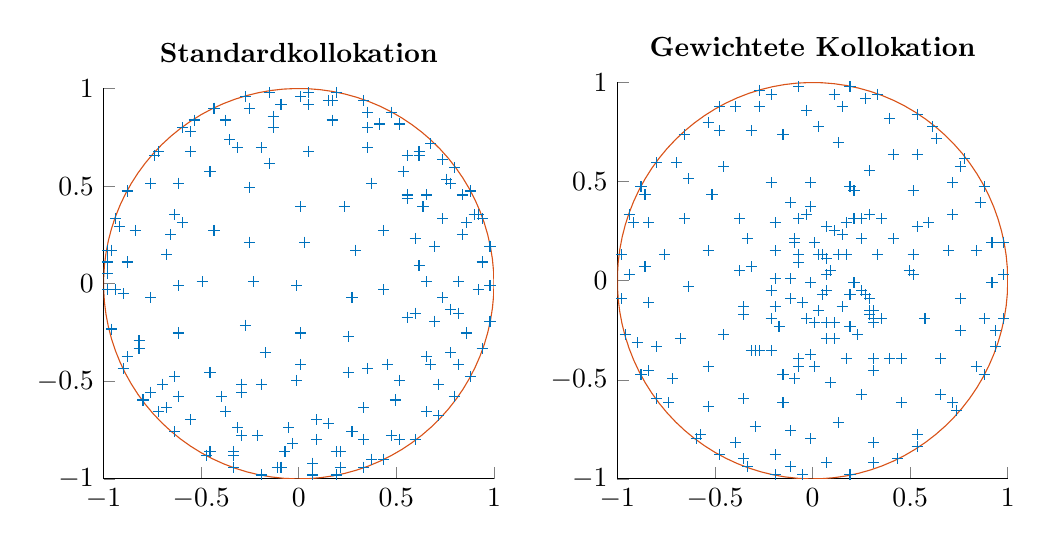
\begin{tikzpicture}

\begin{axis}[%
width=1.952in,
%height=3.566in,
height=1.952in,
at={(0.758in,0.481in)},
scale only axis,
xmin=-1,
xmax=1,
%ymin=-1.82648556876061,
%ymax=1.82648556876061,
ymin=-1,
ymax=1,
axis background/.style={fill=white},
title style={font=\bfseries},
title={Standardkollokation},
axis x line*=bottom,
axis y line*=left,
legend style={legend cell align=left, align=left, draw=white!15!black}
]
\addplot [color=mycolor1, draw=none, mark=+, mark options={solid, mycolor1}]
  table[row sep=crcr]{%
-0.0101010101010101	-0.0101010101010101\\
-0.454545454545455	-0.454545454545455\\
0.878787878787879	0.474747474747475\\
-0.595959595959596	0.797979797979798\\
0.595959595959596	-0.151515151515151\\
-0.252525252525252	0.494949494949495\\
0.878787878787879	-0.474747474747475\\
-0.797979797979798	-0.595959595959596\\
-0.0909090909090909	-0.939393939393939\\
0.0505050505050506	0.97979797979798\\
0.333333333333333	-0.636363636363636\\
0.373737373737374	0.515151515151515\\
-0.97979797979798	0.171717171717172\\
0.434343434343434	-0.898989898989899\\
-0.494949494949495	0.0101010101010102\\
0.474747474747475	0.878787878787879\\
0.97979797979798	-0.0101010101010101\\
-0.0101010101010101	-0.494949494949495\\
0.292929292929293	0.171717171717172\\
-0.878787878787879	0.474747474747475\\
-0.636363636363636	0.353535353535354\\
0.696969696969697	0.191919191919192\\
-0.474747474747475	-0.878787878787879\\
-0.757575757575758	-0.0707070707070707\\
-0.0505050505050505	-0.737373737373737\\
0.656565656565657	-0.656565656565657\\
-0.555555555555556	-0.696969696969697\\
-0.95959595959596	-0.232323232323232\\
0.858585858585859	-0.252525252525252\\
0.171717171717172	0.838383838383838\\
0.616161616161616	0.656565656565657\\
-0.131313131313131	0.797979797979798\\
-0.555555555555556	0.676767676767677\\
-0.272727272727273	0.95959595959596\\
-0.838383838383838	0.272727272727273\\
0.212121212121212	-0.858585858585859\\
0.191919191919192	-0.97979797979798\\
0.858585858585859	0.313131313131313\\
-0.818181818181818	-0.333333333333333\\
0.717171717171717	-0.676767676767677\\
0.676767676767677	0.717171717171717\\
-0.252525252525252	0.212121212121212\\
-0.191919191919192	-0.97979797979798\\
-0.313131313131313	-0.737373737373737\\
-0.939393939393939	-0.0303030303030303\\
0.676767676767677	-0.414141414141414\\
0.0101010101010102	0.393939393939394\\
0.252525252525253	-0.272727272727273\\
0.97979797979798	-0.191919191919192\\
0.0505050505050506	0.676767676767677\\
-0.272727272727273	-0.212121212121212\\
0.97979797979798	0.191919191919192\\
-0.737373737373737	0.656565656565657\\
-0.252525252525252	0.898989898989899\\
-0.757575757575758	0.515151515151515\\
0.191919191919192	0.97979797979798\\
0.818181818181818	0.0101010101010102\\
-0.898989898989899	-0.434343434343434\\
0.454545454545455	-0.414141414141414\\
0.656565656565657	0.454545454545455\\
0.353535353535354	0.696969696969697\\
-0.636363636363636	-0.474747474747475\\
-0.333333333333333	-0.878787878787879\\
-0.676767676767677	0.151515151515152\\
0.434343434343434	-0.0303030303030303\\
-0.353535353535353	0.737373737373737\\
-0.434343434343434	0.272727272727273\\
0.353535353535354	0.878787878787879\\
0.434343434343434	0.272727272727273\\
-0.616161616161616	-0.252525252525252\\
0.474747474747475	-0.777777777777778\\
-0.757575757575758	-0.555555555555556\\
-0.919191919191919	0.292929292929293\\
0.757575757575758	0.535353535353535\\
0.595959595959596	-0.797979797979798\\
0.333333333333333	0.939393939393939\\
0.939393939393939	0.333333333333333\\
-0.434343434343434	0.898989898989899\\
0.0101010101010102	-0.252525252525252\\
-0.939393939393939	0.333333333333333\\
-0.636363636363636	-0.757575757575758\\
-0.97979797979798	-0.0303030303030303\\
-0.616161616161616	0.515151515151515\\
0.0707070707070707	-0.97979797979798\\
-0.191919191919192	-0.515151515151515\\
0.939393939393939	-0.333333333333333\\
-0.595959595959596	0.313131313131313\\
0.212121212121212	-0.939393939393939\\
0.939393939393939	0.111111111111111\\
0.818181818181818	-0.414141414141414\\
0.252525252525253	-0.454545454545455\\
-0.333333333333333	-0.939393939393939\\
-0.0707070707070707	-0.858585858585859\\
0.232323232323232	0.393939393939394\\
0.797979797979798	0.595959595959596\\
0.555555555555556	-0.171717171717172\\
-0.151515151515151	0.97979797979798\\
-0.373737373737374	-0.656565656565657\\
-0.333333333333333	-0.858585858585859\\
0.898989898989899	0.353535353535354\\
-0.717171717171717	-0.656565656565657\\
0.838383838383838	0.454545454545455\\
-0.717171717171717	0.676767676767677\\
-0.454545454545455	0.575757575757576\\
-0.232323232323232	0.0101010101010102\\
0.0303030303030303	0.212121212121212\\
0.494949494949495	-0.595959595959596\\
-0.292929292929293	-0.777777777777778\\
0.171717171717172	0.939393939393939\\
-0.191919191919192	0.696969696969697\\
0.818181818181818	-0.151515151515151\\
0.737373737373737	-0.0707070707070707\\
0.737373737373737	0.333333333333333\\
0.0909090909090908	-0.696969696969697\\
-0.373737373737374	0.838383838383838\\
0.797979797979798	-0.575757575757576\\
0.414141414141414	0.818181818181818\\
0.535353535353535	0.575757575757576\\
-0.171717171717172	-0.353535353535353\\
0.919191919191919	-0.0303030303030303\\
0.515151515151515	0.818181818181818\\
0.555555555555556	0.454545454545455\\
-0.616161616161616	-0.575757575757576\\
0.191919191919192	-0.858585858585859\\
0.151515151515152	0.939393939393939\\
-0.555555555555556	0.777777777777778\\
-0.878787878787879	0.111111111111111\\
-0.131313131313131	0.858585858585859\\
-0.0909090909090909	0.919191919191919\\
-0.616161616161616	-0.0101010101010101\\
0.737373737373737	0.636363636363636\\
0.0707070707070707	-0.919191919191919\\
0.696969696969697	-0.191919191919192\\
-0.878787878787879	-0.373737373737374\\
0.272727272727273	-0.757575757575758\\
0.0101010101010102	-0.414141414141414\\
-0.292929292929293	-0.555555555555556\\
0.272727272727273	-0.0707070707070707\\
-0.454545454545455	-0.858585858585859\\
0.777777777777778	0.515151515151515\\
-0.656565656565657	0.252525252525253\\
0.333333333333333	-0.939393939393939\\
-0.313131313131313	0.696969696969697\\
0.777777777777778	-0.353535353535353\\
-0.95959595959596	0.171717171717172\\
0.555555555555556	0.656565656565657\\
0.777777777777778	-0.131313131313131\\
0.0909090909090908	-0.797979797979798\\
-0.696969696969697	-0.515151515151515\\
0.919191919191919	0.353535353535354\\
0.616161616161616	0.0909090909090908\\
0.838383838383838	0.252525252525253\\
-0.151515151515151	0.616161616161616\\
-0.818181818181818	-0.292929292929293\\
0.0101010101010102	0.95959595959596\\
-0.97979797979798	0.111111111111111\\
0.151515151515152	-0.717171717171717\\
-0.535353535353535	0.838383838383838\\
0.0505050505050506	0.919191919191919\\
0.515151515151515	-0.797979797979798\\
-0.676767676767677	-0.636363636363636\\
0.373737373737374	-0.898989898989899\\
0.717171717171717	-0.515151515151515\\
0.333333333333333	-0.797979797979798\\
0.656565656565657	-0.373737373737374\\
0.515151515151515	-0.494949494949495\\
0.353535353535354	-0.434343434343434\\
0.353535353535354	0.797979797979798\\
0.616161616161616	0.676767676767677\\
-0.898989898989899	-0.0505050505050505\\
-0.97979797979798	0.0505050505050506\\
-0.111111111111111	-0.939393939393939\\
-0.212121212121212	-0.777777777777778\\
-0.292929292929293	-0.515151515151515\\
0.656565656565657	0.0101010101010102\\
-0.0303030303030303	-0.818181818181818\\
0.636363636363636	0.393939393939394\\
0.555555555555556	0.434343434343434\\
0.595959595959596	0.232323232323232\\
-0.393939393939394	-0.575757575757576\\
};
% \addlegendentry{Kollokationspunkte}

\addplot [color=mycolor2, forget plot]
  table[row sep=crcr]{%
1	0\\
0.997986676471884	0.0634239196565645\\
0.991954812830795	0.126592453573749\\
0.981928697262707	0.18925124436041\\
0.967948701396356	0.251147987181079\\
0.950071117740945	0.312033445698487\\
0.928367933016073	0.371662455660328\\
0.902926538286621	0.429794912089172\\
0.873849377069785	0.486196736100469\\
0.841253532831181	0.540640817455598\\
0.805270257531059	0.59290792905464\\
0.766044443118978	0.642787609686539\\
0.72373403810507	0.690079011482112\\
0.678509411557132	0.734591708657533\\
0.630552667084523	0.776146464291757\\
0.580056909571198	0.814575952050336\\
0.527225467610502	0.849725429949514\\
0.472271074772683	0.881453363447582\\
0.415415013001886	0.909631995354518\\
0.356886221591872	0.934147860265107\\
0.296920375328275	0.954902241444074\\
0.235758935509427	0.971811568323542\\
0.173648177666931	0.984807753012208\\
0.110838199901011	0.993838464461254\\
0.0475819158237424	0.998867339183008\\
-0.015865963834808	0.999874127673875\\
-0.0792499568567885	0.996854775951942\\
-0.142314838273285	0.989821441880933\\
-0.204806668065191	0.978802446214779\\
-0.266473813690035	0.963842158559942\\
-0.327067963317421	0.945000818714669\\
-0.386345125693128	0.922354294104581\\
-0.444066612605774	0.895993774291336\\
-0.5	0.866025403784439\\
-0.55392006386611	0.832569854634771\\
-0.605609687137666	0.795761840530832\\
-0.654860733945285	0.755749574354258\\
-0.701474887706321	0.712694171378863\\
-0.745264449675755	0.666769000516292\\
-0.786053094742787	0.618158986220605\\
-0.823676581429833	0.567059863862771\\
-0.857983413234977	0.513677391573407\\
-0.888835448654923	0.458226521727411\\
-0.916108457432069	0.400930535406614\\
-0.939692620785908	0.342020143325669\\
-0.959492973614497	0.28173255684143\\
-0.975429786885407	0.220310532786541\\
-0.987438888676394	0.15800139597335\\
-0.995471922573085	0.0950560433041829\\
-0.999496542383185	0.0317279334980681\\
-0.999496542383185	-0.0317279334980679\\
-0.995471922573085	-0.0950560433041826\\
-0.987438888676394	-0.15800139597335\\
-0.975429786885407	-0.220310532786541\\
-0.959492973614497	-0.281732556841429\\
-0.939692620785908	-0.342020143325669\\
-0.91610845743207	-0.400930535406613\\
-0.888835448654924	-0.45822652172741\\
-0.857983413234977	-0.513677391573406\\
-0.823676581429833	-0.567059863862771\\
-0.786053094742788	-0.618158986220605\\
-0.745264449675755	-0.666769000516292\\
-0.701474887706322	-0.712694171378863\\
-0.654860733945285	-0.755749574354258\\
-0.605609687137667	-0.795761840530832\\
-0.55392006386611	-0.832569854634771\\
-0.5	-0.866025403784438\\
-0.444066612605774	-0.895993774291336\\
-0.386345125693129	-0.922354294104581\\
-0.327067963317422	-0.945000818714668\\
-0.266473813690035	-0.963842158559942\\
-0.204806668065191	-0.978802446214779\\
-0.142314838273285	-0.989821441880933\\
-0.0792499568567888	-0.996854775951942\\
-0.0158659638348076	-0.999874127673875\\
0.0475819158237424	-0.998867339183008\\
0.110838199901011	-0.993838464461254\\
0.17364817766693	-0.984807753012208\\
0.235758935509427	-0.971811568323542\\
0.296920375328275	-0.954902241444074\\
0.356886221591872	-0.934147860265107\\
0.415415013001886	-0.909631995354519\\
0.472271074772682	-0.881453363447582\\
0.527225467610502	-0.849725429949514\\
0.580056909571198	-0.814575952050336\\
0.630552667084522	-0.776146464291757\\
0.678509411557132	-0.734591708657534\\
0.723734038105069	-0.690079011482113\\
0.766044443118977	-0.64278760968654\\
0.805270257531059	-0.59290792905464\\
0.841253532831181	-0.540640817455597\\
0.873849377069785	-0.486196736100469\\
0.902926538286621	-0.429794912089172\\
0.928367933016072	-0.371662455660328\\
0.950071117740945	-0.312033445698487\\
0.967948701396356	-0.251147987181079\\
0.981928697262707	-0.189251244360411\\
0.991954812830795	-0.12659245357375\\
0.997986676471884	-0.0634239196565654\\
1	-2.44929359829471e-16\\
};
\end{axis}

\begin{axis}[%
width=1.952in,
height=1.982in,
at={(3.327in,0.481in)},
scale only axis,
xmin=-1,
xmax=1,
ymin=-1,
ymax=1,
axis background/.style={fill=white},
title style={font=\bfseries},
title={Gewichtete Kollokation},
axis x line*=bottom,
axis y line*=left,
legend style={legend cell align=left, align=left, draw=white!15!black}
]
\addplot [color=mycolor1, draw=none, mark=+, mark options={solid, mycolor1}]
  table[row sep=crcr]{%
-0.0101010101010101	-0.0101010101010101\\
0.878787878787879	0.474747474747475\\
0.535353535353535	0.272727272727273\\
-0.454545454545455	-0.272727272727273\\
-0.878787878787879	-0.474747474747475\\
0.191919191919192	-0.97979797979798\\
0.252525252525253	-0.575757575757576\\
-0.212121212121212	0.494949494949495\\
-0.474747474747475	0.878787878787879\\
0.878787878787879	-0.474747474747475\\
0.333333333333333	0.939393939393939\\
-0.939393939393939	0.333333333333333\\
-0.393939393939394	-0.818181818181818\\
0.575757575757576	-0.191919191919192\\
-0.0707070707070707	0.97979797979798\\
0.535353535353535	-0.838383838383838\\
0.97979797979798	0.0303030303030303\\
-0.656565656565657	0.313131313131313\\
-0.0707070707070707	-0.434343434343434\\
0.191919191919192	0.474747474747475\\
-0.151515151515151	0.737373737373737\\
0.313131313131313	-0.151515151515151\\
-0.373737373737374	0.0505050505050506\\
-0.97979797979798	-0.0909090909090909\\
0.313131313131313	-0.818181818181818\\
0.656565656565657	-0.575757575757576\\
-0.838383838383838	-0.111111111111111\\
-0.111111111111111	-0.757575757575758\\
-0.696969696969697	0.595959595959596\\
0.636363636363636	0.717171717171717\\
0.838383838383838	0.151515151515152\\
-0.797979797979798	0.595959595959596\\
0.414141414141414	0.636363636363636\\
-0.333333333333333	-0.939393939393939\\
-0.595959595959596	-0.797979797979798\\
0.151515151515152	0.878787878787879\\
0.717171717171717	0.494949494949495\\
0.151515151515152	0.232323232323232\\
-0.838383838383838	0.292929292929293\\
-0.717171717171717	-0.494949494949495\\
-0.353535353535353	-0.595959595959596\\
-0.636363636363636	-0.0303030303030303\\
0.878787878787879	-0.191919191919192\\
-0.0505050505050505	-0.97979797979798\\
-0.272727272727273	0.878787878787879\\
0.97979797979798	-0.191919191919192\\
-0.97979797979798	0.131313131313131\\
0.777777777777778	0.616161616161616\\
0.535353535353535	0.838383838383838\\
0.454545454545455	-0.393939393939394\\
0.737373737373737	-0.656565656565657\\
-0.676767676767677	-0.292929292929293\\
-0.454545454545455	0.575757575757576\\
-0.272727272727273	0.95959595959596\\
0.757575757575758	-0.0909090909090909\\
0.656565656565657	-0.393939393939394\\
0.0707070707070707	-0.919191919191919\\
-0.0707070707070707	0.313131313131313\\
0.454545454545455	-0.616161616161616\\
-0.535353535353535	-0.636363636363636\\
-0.212121212121212	-0.191919191919192\\
0.97979797979798	0.191919191919192\\
-0.898989898989899	-0.313131313131313\\
-0.474747474747475	0.757575757575758\\
0.858585858585859	0.393939393939394\\
0.353535353535354	0.313131313131313\\
0.515151515151515	0.454545454545455\\
-0.373737373737374	0.313131313131313\\
0.111111111111111	-0.292929292929293\\
0.191919191919192	0.97979797979798\\
0.393939393939394	0.818181818181818\\
-0.737373737373737	-0.616161616161616\\
0.535353535353535	-0.777777777777778\\
-0.535353535353535	-0.434343434343434\\
-0.191919191919192	-0.878787878787879\\
0.838383838383838	-0.434343434343434\\
0.131313131313131	0.696969696969697\\
0.313131313131313	-0.919191919191919\\
-0.0101010101010101	0.494949494949495\\
-0.797979797979798	-0.595959595959596\\
-0.939393939393939	0.0303030303030303\\
-0.656565656565657	0.737373737373737\\
-0.0303030303030303	0.858585858585859\\
-0.535353535353535	0.151515151515152\\
0.131313131313131	-0.717171717171717\\
0.434343434343434	-0.898989898989899\\
0.111111111111111	0.939393939393939\\
-0.858585858585859	0.434343434343434\\
0.919191919191919	-0.0101010101010101\\
0.515151515151515	0.0303030303030303\\
0.919191919191919	0.191919191919192\\
-0.95959595959596	-0.272727272727273\\
-0.757575757575758	0.131313131313131\\
-0.474747474747475	-0.878787878787879\\
0.212121212121212	-0.0101010101010101\\
-0.313131313131313	0.757575757575758\\
-0.151515151515151	-0.616161616161616\\
0.0909090909090908	-0.515151515151515\\
0.939393939393939	-0.333333333333333\\
-0.636363636363636	0.515151515151515\\
0.696969696969697	0.151515151515152\\
-0.292929292929293	-0.737373737373737\\
0.717171717171717	0.333333333333333\\
0.616161616161616	0.777777777777778\\
-0.313131313131313	-0.353535353535353\\
0.333333333333333	0.131313131313131\\
-0.919191919191919	0.292929292929293\\
-0.353535353535353	-0.898989898989899\\
-0.191919191919192	0.151515151515152\\
0.292929292929293	0.555555555555556\\
-0.797979797979798	-0.333333333333333\\
0.0707070707070707	0.111111111111111\\
0.535353535353535	0.636363636363636\\
-0.575757575757576	-0.777777777777778\\
0.0707070707070707	-0.212121212121212\\
0.191919191919192	-0.0707070707070707\\
0.313131313131313	-0.212121212121212\\
-0.0707070707070707	0.0909090909090908\\
-0.838383838383838	-0.454545454545455\\
0.353535353535354	-0.191919191919192\\
-0.0101010101010101	-0.797979797979798\\
-0.353535353535353	-0.131313131313131\\
-0.333333333333333	0.212121212121212\\
-0.0303030303030303	-0.191919191919192\\
0.595959595959596	0.292929292929293\\
0.272727272727273	-0.0707070707070707\\
0.0303030303030303	0.131313131313131\\
-0.0101010101010101	-0.373737373737374\\
0.171717171717172	-0.393939393939394\\
0.272727272727273	0.919191919191919\\
-0.515151515151515	0.434343434343434\\
0.151515151515152	-0.131313131313131\\
-0.0707070707070707	0.131313131313131\\
0.292929292929293	-0.0909090909090909\\
0.111111111111111	0.252525252525253\\
-0.878787878787879	0.474747474747475\\
-0.151515151515151	-0.474747474747475\\
0.0707070707070707	0.0303030303030303\\
-0.353535353535353	-0.171717171717172\\
-0.0909090909090909	-0.494949494949495\\
0.313131313131313	-0.191919191919192\\
0.191919191919192	-0.232323232323232\\
0.414141414141414	0.212121212121212\\
0.494949494949495	0.0505050505050506\\
-0.0909090909090909	0.212121212121212\\
0.131313131313131	0.131313131313131\\
0.0707070707070707	-0.292929292929293\\
0.292929292929293	-0.151515151515151\\
0.717171717171717	-0.616161616161616\\
0.0101010101010102	0.191919191919192\\
0.393939393939394	-0.393939393939394\\
-0.272727272727273	-0.353535353535353\\
-0.191919191919192	-0.97979797979798\\
-0.212121212121212	0.939393939393939\\
0.0303030303030303	-0.151515151515151\\
-0.171717171717172	-0.232323232323232\\
-0.212121212121212	-0.0505050505050505\\
0.0909090909090908	0.0505050505050506\\
-0.111111111111111	-0.939393939393939\\
0.111111111111111	-0.212121212121212\\
-0.111111111111111	-0.0909090909090909\\
-0.535353535353535	0.797979797979798\\
0.515151515151515	0.131313131313131\\
0.313131313131313	-0.393939393939394\\
0.757575757575758	-0.252525252525252\\
0.171717171717172	0.131313131313131\\
-0.0707070707070707	-0.393939393939394\\
0.313131313131313	-0.454545454545455\\
0.0101010101010102	-0.434343434343434\\
-0.292929292929293	-0.353535353535353\\
-0.191919191919192	-0.131313131313131\\
-0.393939393939394	0.878787878787879\\
-0.0303030303030303	0.333333333333333\\
-0.191919191919192	0.292929292929293\\
0.0707070707070707	0.272727272727273\\
-0.313131313131313	0.0707070707070707\\
-0.212121212121212	-0.353535353535353\\
0.0505050505050506	-0.0707070707070707\\
-0.111111111111111	0.393939393939394\\
0.212121212121212	0.454545454545455\\
-0.191919191919192	0.0101010101010102\\
0.0505050505050506	0.131313131313131\\
0.939393939393939	-0.252525252525252\\
-0.858585858585859	0.0707070707070707\\
0.757575757575758	0.575757575757576\\
0.252525252525253	0.313131313131313\\
0.0303030303030303	0.777777777777778\\
0.252525252525253	-0.0505050505050505\\
0.171717171717172	0.292929292929293\\
0.292929292929293	0.333333333333333\\
0.212121212121212	0.313131313131313\\
0.252525252525253	0.212121212121212\\
-0.0101010101010101	0.373737373737374\\
-0.0505050505050505	-0.111111111111111\\
-0.111111111111111	0.0101010101010102\\
0.0101010101010102	-0.212121212121212\\
0.292929292929293	-0.171717171717172\\
0.0707070707070707	-0.0505050505050505\\
-0.0909090909090909	0.191919191919192\\
0.232323232323232	-0.272727272727273\\
};
%\addlegendentry{Kollokationspunkte}

\addplot [color=mycolor2, forget plot]
  table[row sep=crcr]{%
1	0\\
0.997986676471884	0.0634239196565645\\
0.991954812830795	0.126592453573749\\
0.981928697262707	0.18925124436041\\
0.967948701396356	0.251147987181079\\
0.950071117740945	0.312033445698487\\
0.928367933016073	0.371662455660328\\
0.902926538286621	0.429794912089172\\
0.873849377069785	0.486196736100469\\
0.841253532831181	0.540640817455598\\
0.805270257531059	0.59290792905464\\
0.766044443118978	0.642787609686539\\
0.72373403810507	0.690079011482112\\
0.678509411557132	0.734591708657533\\
0.630552667084523	0.776146464291757\\
0.580056909571198	0.814575952050336\\
0.527225467610502	0.849725429949514\\
0.472271074772683	0.881453363447582\\
0.415415013001886	0.909631995354518\\
0.356886221591872	0.934147860265107\\
0.296920375328275	0.954902241444074\\
0.235758935509427	0.971811568323542\\
0.173648177666931	0.984807753012208\\
0.110838199901011	0.993838464461254\\
0.0475819158237424	0.998867339183008\\
-0.015865963834808	0.999874127673875\\
-0.0792499568567885	0.996854775951942\\
-0.142314838273285	0.989821441880933\\
-0.204806668065191	0.978802446214779\\
-0.266473813690035	0.963842158559942\\
-0.327067963317421	0.945000818714669\\
-0.386345125693128	0.922354294104581\\
-0.444066612605774	0.895993774291336\\
-0.5	0.866025403784439\\
-0.55392006386611	0.832569854634771\\
-0.605609687137666	0.795761840530832\\
-0.654860733945285	0.755749574354258\\
-0.701474887706321	0.712694171378863\\
-0.745264449675755	0.666769000516292\\
-0.786053094742787	0.618158986220605\\
-0.823676581429833	0.567059863862771\\
-0.857983413234977	0.513677391573407\\
-0.888835448654923	0.458226521727411\\
-0.916108457432069	0.400930535406614\\
-0.939692620785908	0.342020143325669\\
-0.959492973614497	0.28173255684143\\
-0.975429786885407	0.220310532786541\\
-0.987438888676394	0.15800139597335\\
-0.995471922573085	0.0950560433041829\\
-0.999496542383185	0.0317279334980681\\
-0.999496542383185	-0.0317279334980679\\
-0.995471922573085	-0.0950560433041826\\
-0.987438888676394	-0.15800139597335\\
-0.975429786885407	-0.220310532786541\\
-0.959492973614497	-0.281732556841429\\
-0.939692620785908	-0.342020143325669\\
-0.91610845743207	-0.400930535406613\\
-0.888835448654924	-0.45822652172741\\
-0.857983413234977	-0.513677391573406\\
-0.823676581429833	-0.567059863862771\\
-0.786053094742788	-0.618158986220605\\
-0.745264449675755	-0.666769000516292\\
-0.701474887706322	-0.712694171378863\\
-0.654860733945285	-0.755749574354258\\
-0.605609687137667	-0.795761840530832\\
-0.55392006386611	-0.832569854634771\\
-0.5	-0.866025403784438\\
-0.444066612605774	-0.895993774291336\\
-0.386345125693129	-0.922354294104581\\
-0.327067963317422	-0.945000818714668\\
-0.266473813690035	-0.963842158559942\\
-0.204806668065191	-0.978802446214779\\
-0.142314838273285	-0.989821441880933\\
-0.0792499568567888	-0.996854775951942\\
-0.0158659638348076	-0.999874127673875\\
0.0475819158237424	-0.998867339183008\\
0.110838199901011	-0.993838464461254\\
0.17364817766693	-0.984807753012208\\
0.235758935509427	-0.971811568323542\\
0.296920375328275	-0.954902241444074\\
0.356886221591872	-0.934147860265107\\
0.415415013001886	-0.909631995354519\\
0.472271074772682	-0.881453363447582\\
0.527225467610502	-0.849725429949514\\
0.580056909571198	-0.814575952050336\\
0.630552667084522	-0.776146464291757\\
0.678509411557132	-0.734591708657534\\
0.723734038105069	-0.690079011482113\\
0.766044443118977	-0.64278760968654\\
0.805270257531059	-0.59290792905464\\
0.841253532831181	-0.540640817455597\\
0.873849377069785	-0.486196736100469\\
0.902926538286621	-0.429794912089172\\
0.928367933016072	-0.371662455660328\\
0.950071117740945	-0.312033445698487\\
0.967948701396356	-0.251147987181079\\
0.981928697262707	-0.189251244360411\\
0.991954812830795	-0.12659245357375\\
0.997986676471884	-0.0634239196565654\\
1	-2.44929359829471e-16\\
};
\end{axis}
\end{tikzpicture}%
}
\caption{Kollokationspunkte beim Greedy-Verfahren bei \acs{PDE} 2}
\label{fig:greedy-points2}
\end{figure}

\subsection{Fehler bei einer anderen Gewichtsfunktion}
\label{sec:andereGewicht}
Wir haben gesehen, dass die gewichteten Verfahren bei der ersten \ac{PDE} vergleichsweise schlechte Ergebnisse liefern. Dies haben wir auf die Gewichtsfunktion zurückgeführt, was nahelegt es mit einer anderen zu versuchen, die keine Singularitäten in den Ecken aufweist. Dafür setzen wir:
\begin{align*}
	w(x) := \sin\left(\frac{\pi}{2}(x_1+1)\right) \sin\left(\frac{\pi}{2}(x_2+1)\right)
\end{align*}
Dies ist keine Gewichtsfunktion im Sinne von \ref{def:gewicht}, da die Funktion außerhalb von $\Omega$ nicht überall kleiner als Null ist. Allerdings sind die Bedingungen in einer Umgebung von $\Omega$ erfüllt. Führen wir mit dieser Funktion die gewichteten Verfahren durch, erhalten wir in Abbildung \ref{fig:andereGewicht} folgenden Fehlerplot:
\begin{figure}[ht]
	\centering
	\resizebox {.85\columnwidth} {!} {
		% This file was created by matlab2tikz.
%
%The latest updates can be retrieved from
%  http://www.mathworks.com/matlabcentral/fileexchange/22022-matlab2tikz-matlab2tikz
%where you can also make suggestions and rate matlab2tikz.
%
%
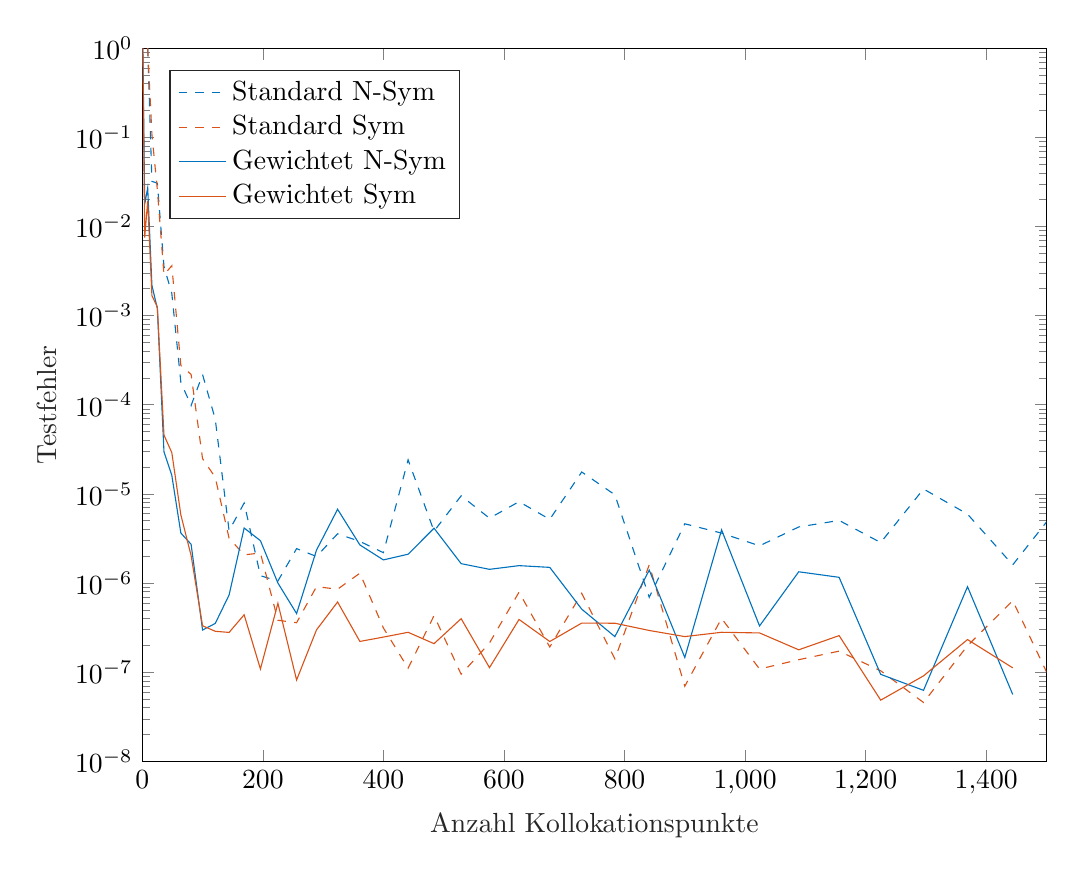
\begin{tikzpicture}

\begin{axis}[%
width=4.521in,
height=3.566in,
at={(0.758in,0.481in)},
scale only axis,
xmin=0,
xmax=1500,
xlabel style={font=\color{white!15!black}},
xlabel={Anzahl Kollokationspunkte},
ymin=1e-8,
ymax=1,
ymode=log,
ylabel style={font=\color{white!15!black}},
ylabel={Testfehler},
axis background/.style={fill=white},
legend style={legend cell align=left, align=left, draw=white!15!black},
legend pos = {north west}
]
\addplot [color=mycolor1, dashed]
  table[row sep=crcr]{%
9	0.999748271191593\\
16	0.0320644506260388\\
25	0.0306339761398731\\
36	0.00355243728244914\\
49	0.0017737871617638\\
64	0.000178468537807508\\
81	9.79655766377152e-05\\
100	0.000218205946323484\\
121	6.93091783866319e-05\\
144	3.87155205178874e-06\\
169	7.89857892615972e-06\\
196	1.20896339392967e-06\\
225	1.05487836936369e-06\\
256	2.43333894801856e-06\\
289	1.98786725878752e-06\\
324	3.56903262012029e-06\\
361	2.93400357476159e-06\\
400	2.19234618849956e-06\\
441	2.41148464918128e-05\\
484	3.82455186892505e-06\\
529	9.52355613608596e-06\\
576	5.34194975650767e-06\\
625	8.18272606923492e-06\\
676	5.18289942128686e-06\\
729	1.76216574033043e-05\\
784	9.77439337927072e-06\\
841	6.92639750311808e-07\\
900	4.61993965032714e-06\\
961	3.63572091333086e-06\\
1024	2.61592994256141e-06\\
1089	4.26045828388899e-06\\
1156	5.0407949436504e-06\\
1225	2.84709437750087e-06\\
1296	1.13539168262317e-05\\
1369	5.9351437327812e-06\\
1444	1.60069958264966e-06\\
1521	7.32080172674565e-06\\
1600	7.33171671805227e-06\\
1681	1.47726674488147e-05\\
1764	4.40686918106586e-06\\
1849	1.22230332882944e-05\\
1936	1.62509643180514e-06\\
2025	7.91387876888233e-06\\
2116	7.15528588670147e-06\\
2209	1.43470301693371e-05\\
2304	7.89284950571123e-06\\
2401	2.46203996043075e-06\\
2500	8.55546425775067e-06\\
2601	2.44848604009917e-06\\
2704	9.7417097966318e-06\\
2809	5.77679670165504e-06\\
2916	5.77146360917352e-06\\
3025	9.06873058542298e-06\\
3136	2.22913705086869e-05\\
3249	1.08550523239409e-05\\
3364	4.80938577396284e-06\\
3481	6.94832855393374e-06\\
3600	1.12212729153349e-05\\
3721	4.09495018619671e-06\\
3844	2.38597305055391e-06\\
3969	4.47799881960267e-06\\
4096	1.89117200467478e-06\\
4225	3.08542426544905e-06\\
4356	4.48144153403912e-06\\
4489	4.76966269510881e-06\\
4624	8.71133417362779e-06\\
4761	6.55746477479235e-06\\
4900	7.21586046274758e-06\\
5041	4.90512203188843e-06\\
5184	7.98014494066135e-06\\
5329	2.46067336308721e-06\\
5476	4.09430751538431e-06\\
5625	5.44380397405134e-06\\
5776	1.4431355321351e-05\\
5929	8.68283233564429e-06\\
6084	9.07630273007734e-06\\
6241	4.01049026368429e-06\\
%6400	1.24298550654191e-05\\
};
\addlegendentry{Standard N-Sym}

\addplot [color=mycolor2, dashed]
  table[row sep=crcr]{%
9	0.999748271191593\\
16	0.107726668816776\\
25	0.0258124696186204\\
36	0.00287159725441316\\
49	0.00362599497445987\\
64	0.000275935163883759\\
81	0.00021918327793681\\
100	2.48216260381184e-05\\
121	1.53681446218856e-05\\
144	3.1884711230723e-06\\
169	2.07364346599404e-06\\
196	2.17226477314258e-06\\
225	3.82458048009404e-07\\
256	3.59086256618291e-07\\
289	9.11238147272009e-07\\
324	8.53447753842995e-07\\
361	1.29068967375662e-06\\
400	3.13765663895182e-07\\
441	1.10766025934739e-07\\
484	4.31307005194226e-07\\
529	9.47970708806145e-08\\
576	2.12821862091706e-07\\
625	7.90592467714291e-07\\
676	1.91874217403409e-07\\
729	7.67803314552506e-07\\
784	1.40958309802208e-07\\
841	1.60128464252868e-06\\
900	6.95889448287801e-08\\
961	4.01987755416222e-07\\
1024	1.08639425788759e-07\\
1089	1.38214763745204e-07\\
1156	1.72387506935934e-07\\
1225	1.03612470492287e-07\\
1296	4.576342060858e-08\\
1369	1.98436127196722e-07\\
1444	6.35113151403743e-07\\
1521	5.06464954974639e-08\\
1600	1.52946966314182e-07\\
1681	4.09538019885414e-07\\
1764	5.5073665183869e-08\\
1849	1.66687766992024e-07\\
1936	1.06468657223857e-07\\
2025	5.50868686666206e-07\\
2116 6.99989677332979e-08\\
2209	1.01204194941085e-07\\
2304	5.08060809312205e-07\\
2401	2.75578998398807e-07\\
2500	1.35024995649713e-07\\
2601	4.28100931787467e-07\\
2704	5.52255797536816e-07\\
2809	3.7940928332425e-07\\
2916	9.61568953350422e-08\\
3025	1.89729150917861e-07\\
3136	1.21232752281486e-07\\
3249	2.27521430473665e-07\\
3364	9.72793279263584e-08\\
3481	2.35286509470134e-07\\
3600 1.68344388165598e-07\\
3721	1.9990815880444e-07\\
3844 1.23043994684074e-07\\
3969 6.10004760037697e-08\\
4096	8.13971327007224e-08\\
4225	6.43811171041619e-08\\
4356	8.52963331077206e-08\\
4489	4.8430353877249e-07\\
4624	9.93239147595304e-08\\
4761	1.89865310695758e-07\\
4900	1.6717591381013e-07\\
5041	6.36370970363842e-08\\
5184	7.78480268026627e-08\\
5329	7.94766711331718e-08\\
5476	1.1111985875889e-07\\
5625	2.43472415561996e-08\\
5776	7.04574397714097e-08\\
5929	5.41579672358461e-08\\
6084	1.31851039864017e-07\\
6241	5.68597048888897e-08\\
%6400	8.04885743610484e-08\\
};
\addlegendentry{Standard Sym}

\addplot [color=mycolor1]
  table[row sep=crcr]{%
1	0.999748271191593\\
4	0.017735844677131\\
9	0.0271266147389331\\
16	0.0021855929958009\\
25	0.00120124891695017\\
36	2.95855313487969e-05\\
49	1.61282517998074e-05\\
64	3.63872619296712e-06\\
81	2.72207136742253e-06\\
100	2.97482806221883e-07\\
121	3.522011861809e-07\\
144	7.33838468436332e-07\\
169	4.14657434567173e-06\\
196	2.98704733139865e-06\\
225	1.00071549963623e-06\\
256	4.55024048551245e-07\\
289	2.34024220566176e-06\\
324	6.72484630603876e-06\\
361	2.67757968647198e-06\\
400	1.8186722921254e-06\\
441	2.10771715704328e-06\\
484	4.12340028274616e-06\\
529	1.65068178986649e-06\\
576	1.42578956371237e-06\\
625	1.56892899189076e-06\\
676	1.49972074998603e-06\\
729	5.09895020872619e-07\\
784	2.50591068742811e-07\\
841	1.39697164419639e-06\\
900	1.46305884143882e-07\\
961	3.94839202373654e-06\\
1024	3.30507332668706e-07\\
1089	1.3384311565467e-06\\
1156	1.15983059209568e-06\\
1225	9.46334275664373e-08\\
1296	6.26393464875363e-08\\
1369	9.10102135102259e-07\\
1444	5.63114703755474e-08\\
};
\addlegendentry{Gewichtet N-Sym}

\addplot [color=mycolor2]
  table[row sep=crcr]{%
1	0.999748271191593\\
4	0.00751068735816518\\
9	0.0193396449785884\\
16	0.00167561975490083\\
25	0.00124953681907569\\
36	4.57317687795888e-05\\
49	2.90374989960207e-05\\
64	5.81403691361781e-06\\
81	2.03245633251248e-06\\
100	3.31958979554736e-07\\
121	2.88001628268031e-07\\
144	2.79440198869274e-07\\
169	4.40901458093057e-07\\
196	1.08677210898869e-07\\
225	5.93005083766862e-07\\
256	8.18230094928873e-08\\
289	2.98357017258777e-07\\
324	6.13252294001665e-07\\
361	2.21454522247866e-07\\
400	2.47760932234851e-07\\
441	2.80398277818783e-07\\
484	2.09086302049855e-07\\
529	3.98764398001905e-07\\
576	1.12581517563298e-07\\
625	3.90628355606548e-07\\
676	2.21144955653285e-07\\
729	3.55796817907289e-07\\
784	3.54477338163073e-07\\
841	2.93962088483701e-07\\
900	2.50989312666761e-07\\
961	2.80462960453032e-07\\
1024	2.75830961043999e-07\\
1089	1.78397169675604e-07\\
1156	2.57351261023775e-07\\
1225	4.8609794633947e-08\\
1296	9.09694937850647e-08\\
1369	2.32457954940646e-07\\
1444	1.11988951057018e-07\\
};
\addlegendentry{Gewichtet Sym}

\end{axis}
\end{tikzpicture}%
	}
	\caption{Testfehler der ersten \acs{PDE} bei einer anderen Gewichtsfunktion}
	\label{fig:andereGewicht}
\end{figure}
Die Kollokationspunkte sind hier wieder auf einem Gitter gewählt. Zum Vergleich sind auch die Testfehler der Standardkollokation nochmal dargestellt. Wir erkennen, dass die gewichtete Kollokation jetzt sehr ähnliche Ergebnisse zur Standardkollokation liefert. Es kann also manchmal hilfreich sein, den theoretisch richtigen Ansatz zu ignorieren und eine eine Funktion zu wählen, die die Bedingungen an eine Gewichtsfunktion nur lokal erfüllt.

\subsection{Fehler auf dem Rand}
Wir werden nun überprüfen, ob die gewichtete Kollokation auch ihren Sinn erfüllt, das heißt ob die Lösung auf dem Rand auch wirklich Null ist. Dafür plotten wir eine mit dem Standardverfahren und eine mit dem gewichteten Verfahren erstellte Lösung der ersten \ac{PDE} in Abbildung \ref{fig:rand-vergleich} über einen Teil des Randes.

\begin{figure}[ht]
\centering
\resizebox {.85\columnwidth} {!} {
% This file was created by matlab2tikz.
%
%The latest updates can be retrieved from
%  http://www.mathworks.com/matlabcentral/fileexchange/22022-matlab2tikz-matlab2tikz
%where you can also make suggestions and rate matlab2tikz.
%
\definecolor{mycolor1}{rgb}{0.00000,0.44700,0.74100}%
\definecolor{mycolor2}{rgb}{0.85000,0.32500,0.09800}%
%
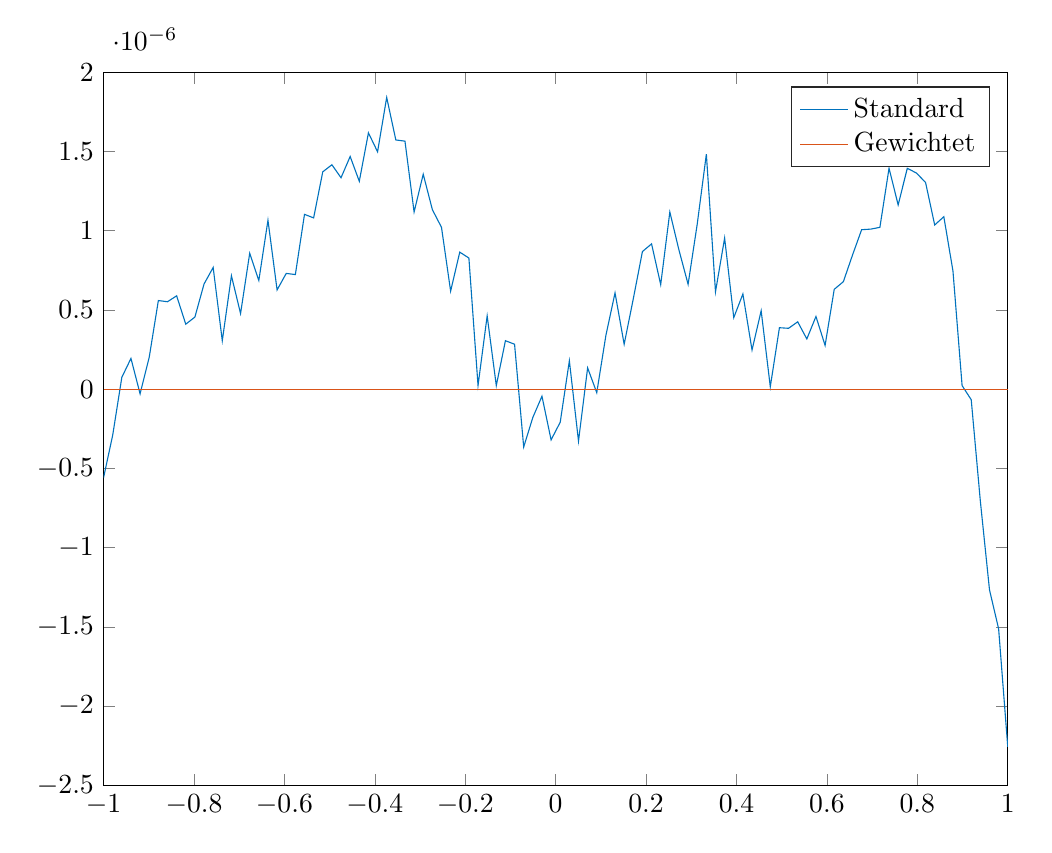
\begin{tikzpicture}

\begin{axis}[%
width=4.521in,
height=3.566in,
at={(0.758in,0.481in)},
scale only axis,
xmin=-1,
xmax=1,
ymin=-2.5e-06,
ymax=2e-06,
axis background/.style={fill=white},
legend style={legend cell align=left, align=left, draw=white!15!black}
]
\addplot [color=mycolor1]
  table[row sep=crcr]{%
-1	-5.58793544769287e-07\\
-0.97979797979798	-2.90572643280029e-07\\
-0.95959595959596	7.45058059692383e-08\\
-0.939393939393939	1.9371509552002e-07\\
-0.919191919191919	-2.98023223876953e-08\\
-0.898989898989899	2.01165676116943e-07\\
-0.878787878787879	5.58793544769287e-07\\
-0.858585858585859	5.51342964172363e-07\\
-0.838383838383838	5.88595867156982e-07\\
-0.818181818181818	4.09781932830811e-07\\
-0.797979797979798	4.54485416412354e-07\\
-0.777777777777778	6.63101673126221e-07\\
-0.757575757575758	7.67409801483154e-07\\
-0.737373737373737	3.05473804473877e-07\\
-0.717171717171717	7.15255737304688e-07\\
-0.696969696969697	4.76837158203125e-07\\
-0.676767676767677	8.5681676864624e-07\\
-0.656565656565657	6.85453414916992e-07\\
-0.636363636363636	1.06543302536011e-06\\
-0.616161616161616	6.25848770141602e-07\\
-0.595959595959596	7.30156898498535e-07\\
-0.575757575757576	7.22706317901611e-07\\
-0.555555555555556	1.10268592834473e-06\\
-0.535353535353535	1.08033418655396e-06\\
-0.515151515151515	1.37090682983398e-06\\
-0.494949494949495	1.41561031341553e-06\\
-0.474747474747475	1.33365392684937e-06\\
-0.454545454545455	1.46776437759399e-06\\
-0.434343434343434	1.31130218505859e-06\\
-0.414141414141414	1.61677598953247e-06\\
-0.393939393939394	1.49756669998169e-06\\
-0.373737373737374	1.84029340744019e-06\\
-0.353535353535353	1.57207250595093e-06\\
-0.333333333333333	1.564621925354e-06\\
-0.313131313131313	1.11758708953857e-06\\
-0.292929292929293	1.35600566864014e-06\\
-0.272727272727273	1.13248825073242e-06\\
-0.252525252525252	1.02072954177856e-06\\
-0.232323232323232	6.18398189544678e-07\\
-0.212121212121212	8.64267349243164e-07\\
-0.191919191919192	8.27014446258545e-07\\
-0.171717171717172	2.23517417907715e-08\\
-0.151515151515151	4.61935997009277e-07\\
-0.131313131313131	2.23517417907715e-08\\
-0.111111111111111	3.05473804473877e-07\\
-0.0909090909090909	2.83122062683105e-07\\
-0.0707070707070707	-3.65078449249268e-07\\
-0.0505050505050505	-1.78813934326172e-07\\
-0.0303030303030303	-4.4703483581543e-08\\
-0.0101010101010101	-3.20374965667725e-07\\
0.0101010101010102	-2.08616256713867e-07\\
0.0303030303030303	1.78813934326172e-07\\
0.0505050505050506	-3.27825546264648e-07\\
0.0707070707070707	1.34110450744629e-07\\
0.0909090909090908	-2.23517417907715e-08\\
0.111111111111111	3.39001417160034e-07\\
0.131313131313131	6.07222318649292e-07\\
0.151515151515152	2.83122062683105e-07\\
0.171717171717172	5.69969415664673e-07\\
0.191919191919192	8.67992639541626e-07\\
0.212121212121212	9.16421413421631e-07\\
0.232323232323232	6.59376382827759e-07\\
0.252525252525253	1.11758708953857e-06\\
0.272727272727273	8.77305865287781e-07\\
0.292929292929293	6.6123902797699e-07\\
0.313131313131313	1.0412186384201e-06\\
0.333333333333333	1.48266553878784e-06\\
0.353535353535354	6.14207237958908e-07\\
0.373737373737374	9.53208655118942e-07\\
0.393939393939394	4.51225787401199e-07\\
0.414141414141414	6.00237399339676e-07\\
0.434343434343434	2.46800482273102e-07\\
0.454545454545455	4.94532287120819e-07\\
0.474747474747475	1.49011611938477e-08\\
0.494949494949495	3.87430191040039e-07\\
0.515151515151515	3.83704900741577e-07\\
0.535353535353535	4.24683094024658e-07\\
0.555555555555556	3.16649675369263e-07\\
0.575757575757576	4.58210706710815e-07\\
0.595959595959596	2.75671482086182e-07\\
0.616161616161616	6.29574060440063e-07\\
0.636363636363636	6.78002834320068e-07\\
0.656565656565657	8.45640897750854e-07\\
0.676767676767677	1.00582838058472e-06\\
0.696969696969697	1.00955367088318e-06\\
0.717171717171717	1.02072954177856e-06\\
0.737373737373737	1.39325857162476e-06\\
0.757575757575758	1.16229057312012e-06\\
0.777777777777778	1.39325857162476e-06\\
0.797979797979798	1.36345624923706e-06\\
0.818181818181818	1.30385160446167e-06\\
0.838383838383838	1.03563070297241e-06\\
0.858585858585859	1.08778476715088e-06\\
0.878787878787879	7.45058059692383e-07\\
0.898989898989899	2.23517417907715e-08\\
0.919191919191919	-6.70552253723145e-08\\
0.939393939393939	-7.07805156707764e-07\\
0.95959595959596	-1.26659870147705e-06\\
0.97979797979798	-1.51246786117554e-06\\
1	-2.25752592086792e-06\\
};
\addlegendentry{Standard}

\addplot [color=mycolor2]
  table[row sep=crcr]{%
-1	0\\
-0.97979797979798	6.36054028626163e-17\\
-0.95959595959596	1.09459696635666e-16\\
-0.939393939393939	-1.96007741793587e-16\\
-0.919191919191919	1.4191549568074e-16\\
-0.898989898989899	-3.71767520242687e-16\\
-0.878787878787879	0\\
-0.858585858585859	0\\
-0.838383838383838	-3.13322411811114e-16\\
-0.818181818181818	0\\
-0.797979797979798	0\\
-0.777777777777778	2.13524025908097e-16\\
-0.757575757575758	0\\
-0.737373737373737	0\\
-0.717171717171717	0\\
-0.696969696969697	0\\
-0.676767676767677	0\\
-0.656565656565657	0\\
-0.636363636363636	3.07819254967142e-16\\
-0.616161616161616	0\\
-0.595959595959596	0\\
-0.575757575757576	0\\
-0.555555555555556	0\\
-0.535353535353535	0\\
-0.515151515151515	0\\
-0.494949494949495	0\\
-0.474747474747475	0\\
-0.454545454545455	0\\
-0.434343434343434	0\\
-0.414141414141414	0\\
-0.393939393939394	3.20741719714877e-16\\
-0.373737373737374	0\\
-0.353535353535353	0\\
-0.333333333333333	0\\
-0.313131313131313	0\\
-0.292929292929293	0\\
-0.272727272727273	0\\
-0.252525252525252	0\\
-0.232323232323232	0\\
-0.212121212121212	0\\
-0.191919191919192	0\\
-0.171717171717172	0\\
-0.151515151515151	0\\
-0.131313131313131	0\\
-0.111111111111111	0\\
-0.0909090909090909	0\\
-0.0707070707070707	0\\
-0.0505050505050505	0\\
-0.0303030303030303	0\\
-0.0101010101010101	0\\
0.0101010101010102	0\\
0.0303030303030303	0\\
0.0505050505050506	0\\
0.0707070707070707	0\\
0.0909090909090908	0\\
0.111111111111111	0\\
0.131313131313131	0\\
0.151515151515152	0\\
0.171717171717172	0\\
0.191919191919192	0\\
0.212121212121212	0\\
0.232323232323232	0\\
0.252525252525253	0\\
0.272727272727273	0\\
0.292929292929293	0\\
0.313131313131313	0\\
0.333333333333333	0\\
0.353535353535354	0\\
0.373737373737374	0\\
0.393939393939394	0\\
0.414141414141414	0\\
0.434343434343434	0\\
0.454545454545455	0\\
0.474747474747475	0\\
0.494949494949495	0\\
0.515151515151515	0\\
0.535353535353535	0\\
0.555555555555556	0\\
0.575757575757576	0\\
0.595959595959596	0\\
0.616161616161616	0\\
0.636363636363636	0\\
0.656565656565657	0\\
0.676767676767677	0\\
0.696969696969697	0\\
0.717171717171717	0\\
0.737373737373737	0\\
0.757575757575758	0\\
0.777777777777778	0\\
0.797979797979798	0\\
0.818181818181818	0\\
0.838383838383838	-1.56661204759499e-16\\
0.858585858585859	0\\
0.878787878787879	0\\
0.898989898989899	3.71767481297e-16\\
0.919191919191919	2.83830927614092e-16\\
0.939393939393939	1.96007644623201e-16\\
0.95959595959596	-1.09459556870653e-16\\
0.97979797979798	-5.08839393738675e-17\\
1	0\\
};
\addlegendentry{Gewichtet}

\end{axis}
\end{tikzpicture}%
}
\caption{Plot über den Rand}
\label{fig:rand-vergleich}
\end{figure}

Bei der Standardkollokation sind deutliche Schwankungen auf dem Rand erkennbar, wohingegen der Rand bei der gewichteten Kollokation tatsächlich Null ist. Das Ziel der gewichteten Kollokation wurde also erreicht.

\subsection{Validationspunkte}
Wir sind bisher nur auf die Wahl der Kollokationspunkte eingegangen, aber noch nicht auf die der Validationspunkte. Dafür stellen wir den Testfehler des nicht-symmetrischen Standardverfahrens und die gewählten $\gamma$-Werte unserer numerischen Lösung der ersten \ac{PDE} in Abbildung \ref{fig:testpunkte} bei gleichbleibenden Kollokationspunkten, aber bei unterschiedlichen Anzahlen von Validationspunkten dar. Beide sind auch hier wieder in einem Gitter angeordnet.
\begin{figure}[ht]
\centering
\resizebox {\columnwidth} {!} {
% This file was created by matlab2tikz.
%
%The latest updates can be retrieved from
%  http://www.mathworks.com/matlabcentral/fileexchange/22022-matlab2tikz-matlab2tikz
%where you can also make suggestions and rate matlab2tikz.
%
%\definecolor{mycolor1}{rgb}{0.00000,0.44700,0.74100}%
%
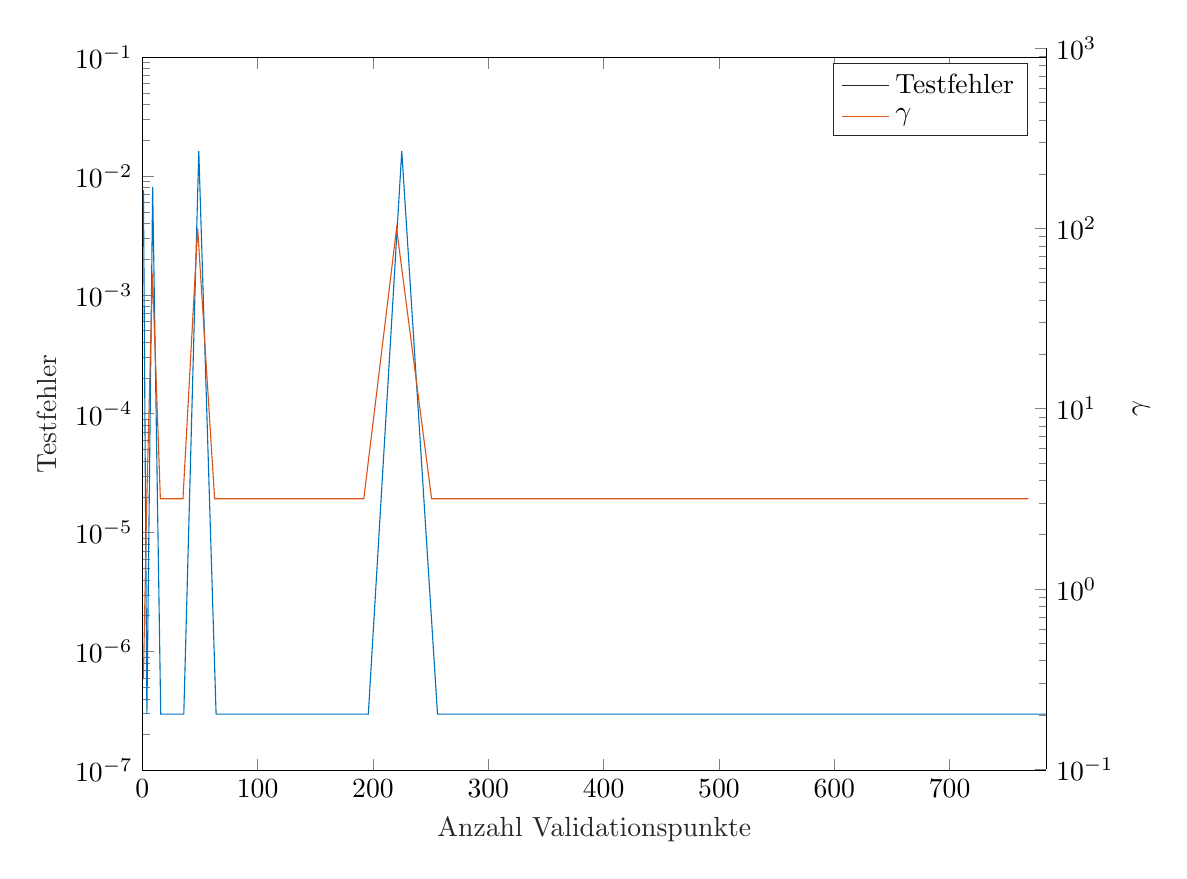
\begin{tikzpicture}

\begin{axis}[%
width=4.521in,
height=3.566in,
at={(0.758in,0.481in)},
scale only axis,
xmin=0,
xmax=784,
xlabel style={font=\color{white!15!black}},
xlabel={Anzahl Validationspunkte},
ymode=log,
ymin=1e-07,
ymax=0.1,
yminorticks=true,
axis y line*=left,
ylabel style={font=\color{white!15!black}},
ylabel={Testfehler},
% axis background/.style={fill=white},
%title style={font=\bfseries},
%title={error plot},
%legend style={legend cell align=left, align=left, draw=white!15!black}
]
\addplot [color=mycolor1]
  table[row sep=crcr]{%
1	0.00760991427227309\\
4	2.97143941410671e-07\\
9	0.00812231198249842\\
16	2.97143941410671e-07\\
25	2.97143941410671e-07\\
36	2.97143941410671e-07\\
49	0.0162268723810862\\
64	2.97143941410671e-07\\
81	2.97143941410671e-07\\
100	2.97143941410671e-07\\
121	2.97143941410671e-07\\
144	2.97143941410671e-07\\
169	2.97143941410671e-07\\
196	2.97143941410671e-07\\
225	0.0162268723810862\\
256	2.97143941410671e-07\\
289	2.97143941410671e-07\\
324	2.97143941410671e-07\\
361	2.97143941410671e-07\\
400	2.97143941410671e-07\\
441	2.97143941410671e-07\\
484	2.97143941410671e-07\\
529	2.97143941410671e-07\\
576	2.97143941410671e-07\\
625	2.97143941410671e-07\\
676	2.97143941410671e-07\\
729	2.97143941410671e-07\\
784	2.97143941410671e-07\\
}; \label{plot_one}
\addlegendentry{Testfehler}

\end{axis}
\begin{axis}[%
width=4.521in,
height=3.605in,
at={(0.758in,0.487in)},
scale only axis,
xmin=0,
xmax=800,
hide x axis,
xlabel style={font=\color{white!15!black}},
xlabel={Anzahl der Testpunkte},
ymode=log,
ymin=0.1,
ymax=1000,
yminorticks=true,
axis y line*=right,
ylabel style={font=\color{white!15!black}},
ylabel={$\gamma$},
ylabel near ticks,
%axis background/.style={fill=white},
%title style={font=\bfseries},
%title={gamma plot},
legend style={legend cell align=left, align=left, draw=white!15!black}
]
\addlegendimage{/pgfplots/refstyle=plot_one}\addlegendentry{Testfehler}
\addplot [color=mycolor2]
  table[row sep=crcr]{%
1	0.316227766016838\\
4	3.16227766016838\\
9	56.2341325190349\\
16	3.16227766016838\\
25	3.16227766016838\\
36	3.16227766016838\\
49	100\\
64	3.16227766016838\\
81	3.16227766016838\\
100	3.16227766016838\\
121	3.16227766016838\\
144	3.16227766016838\\
169	3.16227766016838\\
196	3.16227766016838\\
225	100\\
256	3.16227766016838\\
289	3.16227766016838\\
324	3.16227766016838\\
361	3.16227766016838\\
400	3.16227766016838\\
441	3.16227766016838\\
484	3.16227766016838\\
529	3.16227766016838\\
576	3.16227766016838\\
625	3.16227766016838\\
676	3.16227766016838\\
729	3.16227766016838\\
784	3.16227766016838\\
};
\addlegendentry{$\gamma$}

\end{axis}
\end{tikzpicture}%
}
\caption{Testfehler und $\gamma$-Werte bei unterschiedlichen Anzahlen von Validationspunkten}
\label{fig:testpunkte}
\end{figure}
Wir erkennen, dass der Testfehler bis auf wenige Ausreißer konstant bleibt. Demnach spielt die Wahl der Validationspunkte keine zu große Rolle. Die großen Testfehler entstehen genau dann, wenn alle Validationspunkte mit den Kollokationspunkten zusammenfallen. Den dann auftretenden Effekt nennt man Überanpassung. Die Lösung wird dabei zu gut an die Kollokationspunkte angepasst und verliert dabei an Genauigkeit, wenn alle Testpunkte betrachtet werden. Dabei stellt man fest, dass genau dann, wenn ein großer Fehler auftritt auch ein großes $\gamma$ gewählt wird. Wir erinnern uns an Abbildung \ref{fig:Kerne}, dass ein großes $\gamma$ einem schmalen \glqq Hütchen\grqq{}  der Kernfunktion entspricht. Das kann man so interpretieren, dass, wenn Validations- und Kollokationspunkte zusammenfallen, die Ansatzfunktionen so gewählt werden, dass sie, wenn möglich, nur \glqq Einfluss \grqq{} auf einen Validationspunkt nehmen. Erkennbar ist dies in Abbildung \ref{fig:overfitting}. So entsteht eine Lösung, die an den Testpunkten extrem gut angepasst ist, ansonsten der echten Lösung aber kaum ähnlich sieht.
\begin{figure}[ht]
\centering
\resizebox {\columnwidth} {!} {
% This file was created by matlab2tikz.
%
%The latest updates can be retrieved from
%  http://www.mathworks.com/matlabcentral/fileexchange/22022-matlab2tikz-matlab2tikz
%where you can also make suggestions and rate matlab2tikz.
%
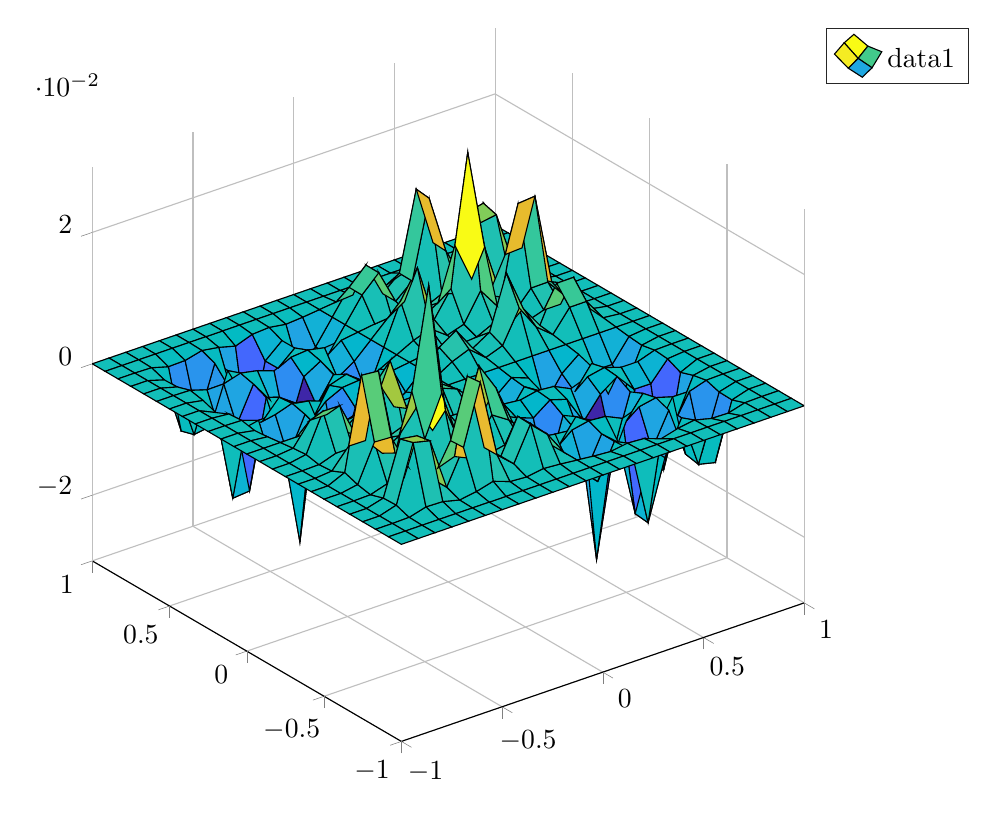
\begin{tikzpicture}

\begin{axis}[%
width=3.56in,
height=3.566in,
at={(0.597in,0.481in)},
scale only axis,
xmin=-1,
xmax=1,
tick align=outside,
ymin=-1,
ymax=1,
zmin=-0.03,
zmax=0.03,
view={-37.5}{30},
axis background/.style={fill=white},
axis x line*=bottom,
axis y line*=left,
axis z line*=left,
xmajorgrids,
ymajorgrids,
zmajorgrids,
legend style={at={(1.03,1)}, anchor=north west, legend cell align=left, align=left, draw=white!15!black}
]

\addplot3[%
surf,
shader=flat corner, draw=black, z buffer=sort, colormap={mymap}{[1pt] rgb(0pt)=(0.2422,0.1504,0.6603); rgb(1pt)=(0.25039,0.164995,0.707614); rgb(2pt)=(0.257771,0.181781,0.751138); rgb(3pt)=(0.264729,0.197757,0.795214); rgb(4pt)=(0.270648,0.214676,0.836371); rgb(5pt)=(0.275114,0.234238,0.870986); rgb(6pt)=(0.2783,0.255871,0.899071); rgb(7pt)=(0.280333,0.278233,0.9221); rgb(8pt)=(0.281338,0.300595,0.941376); rgb(9pt)=(0.281014,0.322757,0.957886); rgb(10pt)=(0.279467,0.344671,0.971676); rgb(11pt)=(0.275971,0.366681,0.982905); rgb(12pt)=(0.269914,0.3892,0.9906); rgb(13pt)=(0.260243,0.412329,0.995157); rgb(14pt)=(0.244033,0.435833,0.998833); rgb(15pt)=(0.220643,0.460257,0.997286); rgb(16pt)=(0.196333,0.484719,0.989152); rgb(17pt)=(0.183405,0.507371,0.979795); rgb(18pt)=(0.178643,0.528857,0.968157); rgb(19pt)=(0.176438,0.549905,0.952019); rgb(20pt)=(0.168743,0.570262,0.935871); rgb(21pt)=(0.154,0.5902,0.9218); rgb(22pt)=(0.146029,0.609119,0.907857); rgb(23pt)=(0.138024,0.627629,0.89729); rgb(24pt)=(0.124814,0.645929,0.888343); rgb(25pt)=(0.111252,0.6635,0.876314); rgb(26pt)=(0.0952095,0.679829,0.859781); rgb(27pt)=(0.0688714,0.694771,0.839357); rgb(28pt)=(0.0296667,0.708167,0.816333); rgb(29pt)=(0.00357143,0.720267,0.7917); rgb(30pt)=(0.00665714,0.731214,0.766014); rgb(31pt)=(0.0433286,0.741095,0.73941); rgb(32pt)=(0.0963952,0.75,0.712038); rgb(33pt)=(0.140771,0.7584,0.684157); rgb(34pt)=(0.1717,0.766962,0.655443); rgb(35pt)=(0.193767,0.775767,0.6251); rgb(36pt)=(0.216086,0.7843,0.5923); rgb(37pt)=(0.246957,0.791795,0.556743); rgb(38pt)=(0.290614,0.79729,0.518829); rgb(39pt)=(0.340643,0.8008,0.478857); rgb(40pt)=(0.3909,0.802871,0.435448); rgb(41pt)=(0.445629,0.802419,0.390919); rgb(42pt)=(0.5044,0.7993,0.348); rgb(43pt)=(0.561562,0.794233,0.304481); rgb(44pt)=(0.617395,0.787619,0.261238); rgb(45pt)=(0.671986,0.779271,0.2227); rgb(46pt)=(0.7242,0.769843,0.191029); rgb(47pt)=(0.773833,0.759805,0.16461); rgb(48pt)=(0.820314,0.749814,0.153529); rgb(49pt)=(0.863433,0.7406,0.159633); rgb(50pt)=(0.903543,0.733029,0.177414); rgb(51pt)=(0.939257,0.728786,0.209957); rgb(52pt)=(0.972757,0.729771,0.239443); rgb(53pt)=(0.995648,0.743371,0.237148); rgb(54pt)=(0.996986,0.765857,0.219943); rgb(55pt)=(0.995205,0.789252,0.202762); rgb(56pt)=(0.9892,0.813567,0.188533); rgb(57pt)=(0.978629,0.838629,0.176557); rgb(58pt)=(0.967648,0.8639,0.16429); rgb(59pt)=(0.96101,0.889019,0.153676); rgb(60pt)=(0.959671,0.913457,0.142257); rgb(61pt)=(0.962795,0.937338,0.12651); rgb(62pt)=(0.969114,0.960629,0.106362); rgb(63pt)=(0.9769,0.9839,0.0805)}, mesh/rows=25]
table[row sep=crcr, point meta=\thisrow{c}] {%
%
x	y	z	c\\
-1	-1	0	0\\
-0.916666666666667	-1	0	0\\
-0.833333333333333	-1	1.02695723625141e-24	1.02695723625141e-24\\
-0.75	-1	0	0\\
-0.666666666666667	-1	0	0\\
-0.583333333333333	-1	0	0\\
-0.5	-1	0	0\\
-0.416666666666667	-1	0	0\\
-0.333333333333333	-1	0	0\\
-0.25	-1	0	0\\
-0.166666666666667	-1	0	0\\
-0.0833333333333334	-1	0	0\\
0	-1	0	0\\
0.0833333333333333	-1	0	0\\
0.166666666666667	-1	0	0\\
0.25	-1	0	0\\
0.333333333333333	-1	0	0\\
0.416666666666667	-1	0	0\\
0.5	-1	0	0\\
0.583333333333333	-1	0	0\\
0.666666666666667	-1	0	0\\
0.75	-1	0	0\\
0.833333333333333	-1	0	0\\
0.916666666666667	-1	-4.38399307163469e-27	-4.38399307163469e-27\\
1	-1	0	0\\
-1	-0.916666666666667	0	0\\
-0.916666666666667	-0.916666666666667	2.55753406345044e-09	2.55753406345044e-09\\
-0.833333333333333	-0.916666666666667	3.85777718973534e-07	3.85777718973534e-07\\
-0.75	-0.916666666666667	4.17100875631788e-06	4.17100875631788e-06\\
-0.666666666666667	-0.916666666666667	3.64929550800072e-06	3.64929550800072e-06\\
-0.583333333333333	-0.916666666666667	3.45860111752149e-07	3.45860111752149e-07\\
-0.5	-0.916666666666667	2.33954300020683e-06	2.33954300020683e-06\\
-0.416666666666667	-0.916666666666667	5.70854139583692e-06	5.70854139583692e-06\\
-0.333333333333333	-0.916666666666667	1.17920908563584e-06	1.17920908563584e-06\\
-0.25	-0.916666666666667	3.45029265806706e-07	3.45029265806706e-07\\
-0.166666666666667	-0.916666666666667	2.26755661545572e-06	2.26755661545572e-06\\
-0.0833333333333334	-0.916666666666667	1.33785564740444e-06	1.33785564740444e-06\\
0	-0.916666666666667	-4.2425755489483e-22	-4.2425755489483e-22\\
0.0833333333333333	-0.916666666666667	-1.33785564740444e-06	-1.33785564740444e-06\\
0.166666666666667	-0.916666666666667	-2.26755661545571e-06	-2.26755661545571e-06\\
0.25	-0.916666666666667	-3.45029265806705e-07	-3.45029265806705e-07\\
0.333333333333333	-0.916666666666667	-1.17920908563584e-06	-1.17920908563584e-06\\
0.416666666666667	-0.916666666666667	-5.70854139583693e-06	-5.70854139583693e-06\\
0.5	-0.916666666666667	-2.33954300020683e-06	-2.33954300020683e-06\\
0.583333333333333	-0.916666666666667	-3.4586011175215e-07	-3.4586011175215e-07\\
0.666666666666667	-0.916666666666667	-3.64929550800072e-06	-3.64929550800072e-06\\
0.75	-0.916666666666667	-4.17100875631788e-06	-4.17100875631788e-06\\
0.833333333333333	-0.916666666666667	-3.85777718973533e-07	-3.85777718973533e-07\\
0.916666666666667	-0.916666666666667	-2.55753406345042e-09	-2.55753406345042e-09\\
1	-0.916666666666667	0	0\\
-1	-0.833333333333333	1.02695723625141e-24	1.02695723625141e-24\\
-0.916666666666667	-0.833333333333333	3.85777718973533e-07	3.85777718973533e-07\\
-0.833333333333333	-0.833333333333333	6.71198962422951e-05	6.71198962422951e-05\\
-0.75	-0.833333333333333	0.000778127800887982	0.000778127800887982\\
-0.666666666666667	-0.833333333333333	0.000707315736756557	0.000707315736756557\\
-0.583333333333333	-0.833333333333333	6.86074746915453e-05	6.86074746915453e-05\\
-0.5	-0.833333333333333	0.000471138162446881	0.000471138162446881\\
-0.416666666666667	-0.833333333333333	0.00116140316014542	0.00116140316014542\\
-0.333333333333333	-0.833333333333333	0.000241610914204461	0.000241610914204461\\
-0.25	-0.833333333333333	7.10368896279139e-05	7.10368896279139e-05\\
-0.166666666666667	-0.833333333333333	0.000468336406285743	0.000468336406285743\\
-0.0833333333333334	-0.833333333333333	0.000276812375771035	0.000276812375771035\\
0	-0.833333333333333	-7.74552301490904e-20	-7.74552301490904e-20\\
0.0833333333333333	-0.833333333333333	-0.000276812375771035	-0.000276812375771035\\
0.166666666666667	-0.833333333333333	-0.000468336406285742	-0.000468336406285742\\
0.25	-0.833333333333333	-7.10368896279136e-05	-7.10368896279136e-05\\
0.333333333333333	-0.833333333333333	-0.00024161091420446	-0.00024161091420446\\
0.416666666666667	-0.833333333333333	-0.00116140316014542	-0.00116140316014542\\
0.5	-0.833333333333333	-0.000471138162446881	-0.000471138162446881\\
0.583333333333333	-0.833333333333333	-6.86074746915456e-05	-6.86074746915456e-05\\
0.666666666666667	-0.833333333333333	-0.000707315736756559	-0.000707315736756559\\
0.75	-0.833333333333333	-0.000778127800887981	-0.000778127800887981\\
0.833333333333333	-0.833333333333333	-6.7119896242295e-05	-6.7119896242295e-05\\
0.916666666666667	-0.833333333333333	-3.85777718973525e-07	-3.85777718973525e-07\\
1	-0.833333333333333	-1.0269572362514e-24	-1.0269572362514e-24\\
-1	-0.75	0	0\\
-0.916666666666667	-0.75	4.17100875631788e-06	4.17100875631788e-06\\
-0.833333333333333	-0.75	0.000778127800887983	0.000778127800887983\\
-0.75	-0.75	0.00943571698715445	0.00943571698715445\\
-0.666666666666667	-0.75	0.00882480124123988	0.00882480124123988\\
-0.583333333333333	-0.75	0.000872104526134152	0.000872104526134152\\
-0.5	-0.75	0.0060652983794619	0.0060652983794619\\
-0.416666666666667	-0.75	0.0150841772008774	0.0150841772008774\\
-0.333333333333333	-0.75	0.00315753528677166	0.00315753528677166\\
-0.25	-0.75	0.000932352964394895	0.000932352964394895\\
-0.166666666666667	-0.75	0.00616423466770155	0.00616423466770155\\
-0.0833333333333334	-0.75	0.00364924259814257	0.00364924259814257\\
0	-0.75	-8.76737641779841e-19	-8.76737641779841e-19\\
0.0833333333333333	-0.75	-0.00364924259814257	-0.00364924259814257\\
0.166666666666667	-0.75	-0.00616423466770154	-0.00616423466770154\\
0.25	-0.75	-0.000932352964394891	-0.000932352964394891\\
0.333333333333333	-0.75	-0.00315753528677164	-0.00315753528677164\\
0.416666666666667	-0.75	-0.0150841772008774	-0.0150841772008774\\
0.5	-0.75	-0.0060652983794619	-0.0060652983794619\\
0.583333333333333	-0.75	-0.000872104526134156	-0.000872104526134156\\
0.666666666666667	-0.75	-0.00882480124123989	-0.00882480124123989\\
0.75	-0.75	-0.00943571698715444	-0.00943571698715444\\
0.833333333333333	-0.75	-0.000778127800887982	-0.000778127800887982\\
0.916666666666667	-0.75	-4.17100875631781e-06	-4.17100875631781e-06\\
1	-0.75	0	0\\
-1	-0.666666666666667	0	0\\
-0.916666666666667	-0.666666666666667	3.64929550800072e-06	3.64929550800072e-06\\
-0.833333333333333	-0.666666666666667	0.000707315736756557	0.000707315736756557\\
-0.75	-0.666666666666667	0.00882480124123988	0.00882480124123988\\
-0.666666666666667	-0.666666666666667	0.00842066215543398	0.00842066215543398\\
-0.583333333333333	-0.666666666666667	0.000843966898384536	0.000843966898384536\\
-0.5	-0.666666666666667	0.00592857826938018	0.00592857826938018\\
-0.416666666666667	-0.666666666666667	0.0148502404760497	0.0148502404760497\\
-0.333333333333333	-0.666666666666667	0.00312456184123599	0.00312456184123599\\
-0.25	-0.666666666666667	0.000925942478032866	0.000925942478032866\\
-0.166666666666667	-0.666666666666667	0.00613646636398126	0.00613646636398126\\
-0.0833333333333334	-0.666666666666667	0.00363775449063844	0.00363775449063844\\
0	-0.666666666666667	-8.44331861748012e-19	-8.44331861748012e-19\\
0.0833333333333333	-0.666666666666667	-0.00363775449063844	-0.00363775449063844\\
0.166666666666667	-0.666666666666667	-0.00613646636398124	-0.00613646636398124\\
0.25	-0.666666666666667	-0.000925942478032862	-0.000925942478032862\\
0.333333333333333	-0.666666666666667	-0.00312456184123597	-0.00312456184123597\\
0.416666666666667	-0.666666666666667	-0.0148502404760497	-0.0148502404760497\\
0.5	-0.666666666666667	-0.00592857826938018	-0.00592857826938018\\
0.583333333333333	-0.666666666666667	-0.00084396689838454	-0.00084396689838454\\
0.666666666666667	-0.666666666666667	-0.00842066215543399	-0.00842066215543399\\
0.75	-0.666666666666667	-0.00882480124123987	-0.00882480124123987\\
0.833333333333333	-0.666666666666667	-0.000707315736756558	-0.000707315736756558\\
0.916666666666667	-0.666666666666667	-3.64929550800066e-06	-3.64929550800066e-06\\
1	-0.666666666666667	0	0\\
-1	-0.583333333333333	0	0\\
-0.916666666666667	-0.583333333333333	3.45860111752149e-07	3.45860111752149e-07\\
-0.833333333333333	-0.583333333333333	6.86074746915453e-05	6.86074746915453e-05\\
-0.75	-0.583333333333333	0.000872104526134152	0.000872104526134152\\
-0.666666666666667	-0.583333333333333	0.000843966898384536	0.000843966898384536\\
-0.583333333333333	-0.583333333333333	8.50681297213606e-05	8.50681297213606e-05\\
-0.5	-0.583333333333333	0.000592761470027727	0.000592761470027727\\
-0.416666666666667	-0.583333333333333	0.00149315597727987	0.00149315597727987\\
-0.333333333333333	-0.583333333333333	0.000315453871556334	0.000315453871556334\\
-0.25	-0.583333333333333	9.31814902686496e-05	9.31814902686496e-05\\
-0.166666666666667	-0.583333333333333	0.000618502248354859	0.000618502248354859\\
-0.0833333333333334	-0.583333333333333	0.000367064223668659	0.000367064223668659\\
0	-0.583333333333333	-7.40930762219607e-20	-7.40930762219607e-20\\
0.0833333333333333	-0.583333333333333	-0.000367064223668659	-0.000367064223668659\\
0.166666666666667	-0.583333333333333	-0.000618502248354857	-0.000618502248354857\\
0.25	-0.583333333333333	-9.31814902686491e-05	-9.31814902686491e-05\\
0.333333333333333	-0.583333333333333	-0.000315453871556332	-0.000315453871556332\\
0.416666666666667	-0.583333333333333	-0.00149315597727987	-0.00149315597727987\\
0.5	-0.583333333333333	-0.000592761470027727	-0.000592761470027727\\
0.583333333333333	-0.583333333333333	-8.50681297213611e-05	-8.50681297213611e-05\\
0.666666666666667	-0.583333333333333	-0.000843966898384538	-0.000843966898384538\\
0.75	-0.583333333333333	-0.00087210452613415	-0.00087210452613415\\
0.833333333333333	-0.583333333333333	-6.86074746915454e-05	-6.86074746915454e-05\\
0.916666666666667	-0.583333333333333	-3.45860111752143e-07	-3.45860111752143e-07\\
1	-0.583333333333333	0	0\\
-1	-0.5	0	0\\
-0.916666666666667	-0.5	2.33954300020683e-06	2.33954300020683e-06\\
-0.833333333333333	-0.5	0.000471138162446881	0.000471138162446881\\
-0.75	-0.5	0.0060652983794619	0.0060652983794619\\
-0.666666666666667	-0.5	0.00592857826938018	0.00592857826938018\\
-0.583333333333333	-0.5	0.000592761470027727	0.000592761470027727\\
-0.5	-0.5	0.00393294666281547	0.00393294666281547\\
-0.416666666666667	-0.5	0.00994977833558941	0.00994977833558941\\
-0.333333333333333	-0.5	0.00210867680461956	0.00210867680461956\\
-0.25	-0.5	0.000610455051438689	0.000610455051438689\\
-0.166666666666667	-0.5	0.00405241439845992	0.00405241439845992\\
-0.0833333333333334	-0.5	0.0024071556172955	0.0024071556172955\\
0	-0.5	-5.91805759022251e-19	-5.91805759022251e-19\\
0.0833333333333333	-0.5	-0.0024071556172955	-0.0024071556172955\\
0.166666666666667	-0.5	-0.00405241439845991	-0.00405241439845991\\
0.25	-0.5	-0.000610455051438686	-0.000610455051438686\\
0.333333333333333	-0.5	-0.00210867680461956	-0.00210867680461956\\
0.416666666666667	-0.5	-0.00994977833558942	-0.00994977833558942\\
0.5	-0.5	-0.00393294666281547	-0.00393294666281547\\
0.583333333333333	-0.5	-0.000592761470027729	-0.000592761470027729\\
0.666666666666667	-0.5	-0.00592857826938019	-0.00592857826938019\\
0.75	-0.5	-0.00606529837946189	-0.00606529837946189\\
0.833333333333333	-0.5	-0.000471138162446881	-0.000471138162446881\\
0.916666666666667	-0.5	-2.33954300020679e-06	-2.33954300020679e-06\\
1	-0.5	0	0\\
-1	-0.416666666666667	0	0\\
-0.916666666666667	-0.416666666666667	5.70854139583692e-06	5.70854139583692e-06\\
-0.833333333333333	-0.416666666666667	0.00116140316014542	0.00116140316014542\\
-0.75	-0.416666666666667	0.0150841772008774	0.0150841772008774\\
-0.666666666666667	-0.416666666666667	0.0148502404760497	0.0148502404760497\\
-0.583333333333333	-0.416666666666667	0.00149315597727987	0.00149315597727987\\
-0.5	-0.416666666666667	0.00994977833558941	0.00994977833558941\\
-0.416666666666667	-0.416666666666667	0.0252552578198303	0.0252552578198303\\
-0.333333333333333	-0.416666666666667	0.00536572588063085	0.00536572588063085\\
-0.25	-0.416666666666667	0.00155612453270233	0.00155612453270233\\
-0.166666666666667	-0.416666666666667	0.010342674976464	0.010342674976464\\
-0.0833333333333334	-0.416666666666667	0.00614793627719881	0.00614793627719881\\
0	-0.416666666666667	-1.50433859765667e-18	-1.50433859765667e-18\\
0.0833333333333333	-0.416666666666667	-0.0061479362771988	-0.0061479362771988\\
0.166666666666667	-0.416666666666667	-0.010342674976464	-0.010342674976464\\
0.25	-0.416666666666667	-0.00155612453270232	-0.00155612453270232\\
0.333333333333333	-0.416666666666667	-0.00536572588063083	-0.00536572588063083\\
0.416666666666667	-0.416666666666667	-0.0252552578198304	-0.0252552578198304\\
0.5	-0.416666666666667	-0.00994977833558941	-0.00994977833558941\\
0.583333333333333	-0.416666666666667	-0.00149315597727988	-0.00149315597727988\\
0.666666666666667	-0.416666666666667	-0.0148502404760497	-0.0148502404760497\\
0.75	-0.416666666666667	-0.0150841772008774	-0.0150841772008774\\
0.833333333333333	-0.416666666666667	-0.00116140316014542	-0.00116140316014542\\
0.916666666666667	-0.416666666666667	-5.70854139583682e-06	-5.70854139583682e-06\\
1	-0.416666666666667	0	0\\
-1	-0.333333333333333	0	0\\
-0.916666666666667	-0.333333333333333	1.17920908563584e-06	1.17920908563584e-06\\
-0.833333333333333	-0.333333333333333	0.000241610914204461	0.000241610914204461\\
-0.75	-0.333333333333333	0.00315753528677166	0.00315753528677166\\
-0.666666666666667	-0.333333333333333	0.00312456184123599	0.00312456184123599\\
-0.583333333333333	-0.333333333333333	0.000315453871556334	0.000315453871556334\\
-0.5	-0.333333333333333	0.00210867680461956	0.00210867680461956\\
-0.416666666666667	-0.333333333333333	0.00536572588063085	0.00536572588063085\\
-0.333333333333333	-0.333333333333333	0.00114214387023767	0.00114214387023767\\
-0.25	-0.333333333333333	0.000331677317790113	0.000331677317790113\\
-0.166666666666667	-0.333333333333333	0.00220651736235955	0.00220651736235955\\
-0.0833333333333334	-0.333333333333333	0.00131231582712499	0.00131231582712499\\
0	-0.333333333333333	-3.16585135024486e-19	-3.16585135024486e-19\\
0.0833333333333333	-0.333333333333333	-0.00131231582712499	-0.00131231582712499\\
0.166666666666667	-0.333333333333333	-0.00220651736235954	-0.00220651736235954\\
0.25	-0.333333333333333	-0.000331677317790112	-0.000331677317790112\\
0.333333333333333	-0.333333333333333	-0.00114214387023766	-0.00114214387023766\\
0.416666666666667	-0.333333333333333	-0.00536572588063086	-0.00536572588063086\\
0.5	-0.333333333333333	-0.00210867680461956	-0.00210867680461956\\
0.583333333333333	-0.333333333333333	-0.000315453871556335	-0.000315453871556335\\
0.666666666666667	-0.333333333333333	-0.00312456184123599	-0.00312456184123599\\
0.75	-0.333333333333333	-0.00315753528677165	-0.00315753528677165\\
0.833333333333333	-0.333333333333333	-0.000241610914204461	-0.000241610914204461\\
0.916666666666667	-0.333333333333333	-1.17920908563582e-06	-1.17920908563582e-06\\
1	-0.333333333333333	0	0\\
-1	-0.25	0	0\\
-0.916666666666667	-0.25	3.45029265806706e-07	3.45029265806706e-07\\
-0.833333333333333	-0.25	7.1036889627914e-05	7.1036889627914e-05\\
-0.75	-0.25	0.000932352964394894	0.000932352964394894\\
-0.666666666666667	-0.25	0.000925942478032866	0.000925942478032866\\
-0.583333333333333	-0.25	9.31814902686495e-05	9.31814902686495e-05\\
-0.5	-0.25	0.000610455051438689	0.000610455051438689\\
-0.416666666666667	-0.25	0.00155612453270233	0.00155612453270233\\
-0.333333333333333	-0.25	0.000331677317790113	0.000331677317790113\\
-0.25	-0.25	9.54350634367825e-05	9.54350634367825e-05\\
-0.166666666666667	-0.25	0.000634901021554919	0.000634901021554919\\
-0.0833333333333334	-0.25	0.00037775454883306	0.00037775454883306\\
0	-0.25	-8.80499813311504e-20	-8.80499813311504e-20\\
0.0833333333333333	-0.25	-0.00037775454883306	-0.00037775454883306\\
0.166666666666667	-0.25	-0.000634901021554917	-0.000634901021554917\\
0.25	-0.25	-9.54350634367821e-05	-9.54350634367821e-05\\
0.333333333333333	-0.25	-0.000331677317790112	-0.000331677317790112\\
0.416666666666667	-0.25	-0.00155612453270233	-0.00155612453270233\\
0.5	-0.25	-0.000610455051438689	-0.000610455051438689\\
0.583333333333333	-0.25	-9.31814902686498e-05	-9.31814902686498e-05\\
0.666666666666667	-0.25	-0.000925942478032867	-0.000925942478032867\\
0.75	-0.25	-0.000932352964394893	-0.000932352964394893\\
0.833333333333333	-0.25	-7.1036889627914e-05	-7.1036889627914e-05\\
0.916666666666667	-0.25	-3.450292658067e-07	-3.450292658067e-07\\
1	-0.25	0	0\\
-1	-0.166666666666667	0	0\\
-0.916666666666667	-0.166666666666667	2.26755661545572e-06	2.26755661545572e-06\\
-0.833333333333333	-0.166666666666667	0.000468336406285743	0.000468336406285743\\
-0.75	-0.166666666666667	0.00616423466770155	0.00616423466770155\\
-0.666666666666667	-0.166666666666667	0.00613646636398126	0.00613646636398126\\
-0.583333333333333	-0.166666666666667	0.000618502248354858	0.000618502248354858\\
-0.5	-0.166666666666667	0.00405241439845992	0.00405241439845992\\
-0.416666666666667	-0.166666666666667	0.010342674976464	0.010342674976464\\
-0.333333333333333	-0.166666666666667	0.00220651736235955	0.00220651736235955\\
-0.25	-0.166666666666667	0.000634901021554919	0.000634901021554919\\
-0.166666666666667	-0.166666666666667	0.00422559650685534	0.00422559650685534\\
-0.0833333333333334	-0.166666666666667	0.00251483803933617	0.00251483803933617\\
0	-0.166666666666667	-6.34758211468699e-19	-6.34758211468699e-19\\
0.0833333333333333	-0.166666666666667	-0.00251483803933617	-0.00251483803933617\\
0.166666666666667	-0.166666666666667	-0.00422559650685533	-0.00422559650685533\\
0.25	-0.166666666666667	-0.000634901021554916	-0.000634901021554916\\
0.333333333333333	-0.166666666666667	-0.00220651736235954	-0.00220651736235954\\
0.416666666666667	-0.166666666666667	-0.010342674976464	-0.010342674976464\\
0.5	-0.166666666666667	-0.00405241439845992	-0.00405241439845992\\
0.583333333333333	-0.166666666666667	-0.000618502248354861	-0.000618502248354861\\
0.666666666666667	-0.166666666666667	-0.00613646636398127	-0.00613646636398127\\
0.75	-0.166666666666667	-0.00616423466770154	-0.00616423466770154\\
0.833333333333333	-0.166666666666667	-0.000468336406285743	-0.000468336406285743\\
0.916666666666667	-0.166666666666667	-2.26755661545568e-06	-2.26755661545568e-06\\
1	-0.166666666666667	0	0\\
-1	-0.0833333333333334	0	0\\
-0.916666666666667	-0.0833333333333334	1.33785564740444e-06	1.33785564740444e-06\\
-0.833333333333333	-0.0833333333333334	0.000276812375771035	0.000276812375771035\\
-0.75	-0.0833333333333334	0.00364924259814257	0.00364924259814257\\
-0.666666666666667	-0.0833333333333334	0.00363775449063844	0.00363775449063844\\
-0.583333333333333	-0.0833333333333334	0.000367064223668659	0.000367064223668659\\
-0.5	-0.0833333333333334	0.0024071556172955	0.0024071556172955\\
-0.416666666666667	-0.0833333333333334	0.0061479362771988	0.0061479362771988\\
-0.333333333333333	-0.0833333333333334	0.00131231582712499	0.00131231582712499\\
-0.25	-0.0833333333333334	0.00037775454883306	0.00037775454883306\\
-0.166666666666667	-0.0833333333333334	0.00251483803933617	0.00251483803933617\\
-0.0833333333333334	-0.0833333333333334	0.0014969284339611	0.0014969284339611\\
0	-0.0833333333333334	-4.12134423225633e-19	-4.12134423225633e-19\\
0.0833333333333333	-0.0833333333333334	-0.0014969284339611	-0.0014969284339611\\
0.166666666666667	-0.0833333333333334	-0.00251483803933616	-0.00251483803933616\\
0.25	-0.0833333333333334	-0.000377754548833058	-0.000377754548833058\\
0.333333333333333	-0.0833333333333334	-0.00131231582712498	-0.00131231582712498\\
0.416666666666667	-0.0833333333333334	-0.00614793627719881	-0.00614793627719881\\
0.5	-0.0833333333333334	-0.00240715561729551	-0.00240715561729551\\
0.583333333333333	-0.0833333333333334	-0.000367064223668661	-0.000367064223668661\\
0.666666666666667	-0.0833333333333334	-0.00363775449063844	-0.00363775449063844\\
0.75	-0.0833333333333334	-0.00364924259814256	-0.00364924259814256\\
0.833333333333333	-0.0833333333333334	-0.000276812375771035	-0.000276812375771035\\
0.916666666666667	-0.0833333333333334	-1.33785564740442e-06	-1.33785564740442e-06\\
1	-0.0833333333333334	0	0\\
-1	0	0	0\\
-0.916666666666667	0	-4.22019650749432e-22	-4.22019650749432e-22\\
-0.833333333333333	0	-7.58062703141482e-20	-7.58062703141482e-20\\
-0.75	0	-8.8948973557021e-19	-8.8948973557021e-19\\
-0.666666666666667	0	-8.48925864908015e-19	-8.48925864908015e-19\\
-0.583333333333333	0	-7.4663668535476e-20	-7.4663668535476e-20\\
-0.5	0	-6.59299545930563e-19	-6.59299545930563e-19\\
-0.416666666666667	0	-1.65655633099897e-18	-1.65655633099897e-18\\
-0.333333333333333	0	-3.57084812293917e-19	-3.57084812293917e-19\\
-0.25	0	-8.37743870326049e-20	-8.37743870326049e-20\\
-0.166666666666667	0	-6.03879200828298e-19	-6.03879200828298e-19\\
-0.0833333333333334	0	-3.932851103973e-19	-3.932851103973e-19\\
0	0	-4.82118586296267e-21	-4.82118586296267e-21\\
0.0833333333333333	0	4.48056541275829e-19	4.48056541275829e-19\\
0.166666666666667	0	6.75165917404855e-19	6.75165917404855e-19\\
0.25	0	8.05379513898792e-20	8.05379513898792e-20\\
0.333333333333333	0	3.00487456194101e-19	3.00487456194101e-19\\
0.416666666666667	0	1.62580333661468e-18	1.62580333661468e-18\\
0.5	0	5.57212921187685e-19	5.57212921187685e-19\\
0.583333333333333	0	9.80093456331336e-20	9.80093456331336e-20\\
0.666666666666667	0	8.61737011716055e-19	8.61737011716055e-19\\
0.75	0	9.60761298722394e-19	9.60761298722394e-19\\
0.833333333333333	0	7.99192795843061e-20	7.99192795843061e-20\\
0.916666666666667	0	3.15236993062634e-22	3.15236993062634e-22\\
1	0	0	0\\
-1	0.0833333333333333	0	0\\
-0.916666666666667	0.0833333333333333	-1.33785564740444e-06	-1.33785564740444e-06\\
-0.833333333333333	0.0833333333333333	-0.000276812375771035	-0.000276812375771035\\
-0.75	0.0833333333333333	-0.00364924259814257	-0.00364924259814257\\
-0.666666666666667	0.0833333333333333	-0.00363775449063844	-0.00363775449063844\\
-0.583333333333333	0.0833333333333333	-0.000367064223668659	-0.000367064223668659\\
-0.5	0.0833333333333333	-0.0024071556172955	-0.0024071556172955\\
-0.416666666666667	0.0833333333333333	-0.0061479362771988	-0.0061479362771988\\
-0.333333333333333	0.0833333333333333	-0.00131231582712499	-0.00131231582712499\\
-0.25	0.0833333333333333	-0.00037775454883306	-0.00037775454883306\\
-0.166666666666667	0.0833333333333333	-0.00251483803933617	-0.00251483803933617\\
-0.0833333333333334	0.0833333333333333	-0.0014969284339611	-0.0014969284339611\\
0	0.0833333333333333	4.51410925247731e-19	4.51410925247731e-19\\
0.0833333333333333	0.0833333333333333	0.0014969284339611	0.0014969284339611\\
0.166666666666667	0.0833333333333333	0.00251483803933616	0.00251483803933616\\
0.25	0.0833333333333333	0.000377754548833058	0.000377754548833058\\
0.333333333333333	0.0833333333333333	0.00131231582712498	0.00131231582712498\\
0.416666666666667	0.0833333333333333	0.00614793627719881	0.00614793627719881\\
0.5	0.0833333333333333	0.0024071556172955	0.0024071556172955\\
0.583333333333333	0.0833333333333333	0.00036706422366866	0.00036706422366866\\
0.666666666666667	0.0833333333333333	0.00363775449063844	0.00363775449063844\\
0.75	0.0833333333333333	0.00364924259814256	0.00364924259814256\\
0.833333333333333	0.0833333333333333	0.000276812375771035	0.000276812375771035\\
0.916666666666667	0.0833333333333333	1.33785564740442e-06	1.33785564740442e-06\\
1	0.0833333333333333	0	0\\
-1	0.166666666666667	0	0\\
-0.916666666666667	0.166666666666667	-2.26755661545571e-06	-2.26755661545571e-06\\
-0.833333333333333	0.166666666666667	-0.000468336406285741	-0.000468336406285741\\
-0.75	0.166666666666667	-0.00616423466770153	-0.00616423466770153\\
-0.666666666666667	0.166666666666667	-0.00613646636398124	-0.00613646636398124\\
-0.583333333333333	0.166666666666667	-0.000618502248354857	-0.000618502248354857\\
-0.5	0.166666666666667	-0.00405241439845991	-0.00405241439845991\\
-0.416666666666667	0.166666666666667	-0.010342674976464	-0.010342674976464\\
-0.333333333333333	0.166666666666667	-0.00220651736235954	-0.00220651736235954\\
-0.25	0.166666666666667	-0.000634901021554917	-0.000634901021554917\\
-0.166666666666667	0.166666666666667	-0.00422559650685533	-0.00422559650685533\\
-0.0833333333333334	0.166666666666667	-0.00251483803933616	-0.00251483803933616\\
0	0.166666666666667	6.9848421185914e-19	6.9848421185914e-19\\
0.0833333333333333	0.166666666666667	0.00251483803933616	0.00251483803933616\\
0.166666666666667	0.166666666666667	0.00422559650685532	0.00422559650685532\\
0.25	0.166666666666667	0.000634901021554914	0.000634901021554914\\
0.333333333333333	0.166666666666667	0.00220651736235953	0.00220651736235953\\
0.416666666666667	0.166666666666667	0.010342674976464	0.010342674976464\\
0.5	0.166666666666667	0.00405241439845991	0.00405241439845991\\
0.583333333333333	0.166666666666667	0.000618502248354859	0.000618502248354859\\
0.666666666666667	0.166666666666667	0.00613646636398125	0.00613646636398125\\
0.75	0.166666666666667	0.00616423466770152	0.00616423466770152\\
0.833333333333333	0.166666666666667	0.000468336406285741	0.000468336406285741\\
0.916666666666667	0.166666666666667	2.26755661545567e-06	2.26755661545567e-06\\
1	0.166666666666667	0	0\\
-1	0.25	0	0\\
-0.916666666666667	0.25	-3.45029265806704e-07	-3.45029265806704e-07\\
-0.833333333333333	0.25	-7.10368896279136e-05	-7.10368896279136e-05\\
-0.75	0.25	-0.000932352964394891	-0.000932352964394891\\
-0.666666666666667	0.25	-0.000925942478032862	-0.000925942478032862\\
-0.583333333333333	0.25	-9.31814902686491e-05	-9.31814902686491e-05\\
-0.5	0.25	-0.000610455051438686	-0.000610455051438686\\
-0.416666666666667	0.25	-0.00155612453270232	-0.00155612453270232\\
-0.333333333333333	0.25	-0.000331677317790112	-0.000331677317790112\\
-0.25	0.25	-9.5435063436782e-05	-9.5435063436782e-05\\
-0.166666666666667	0.25	-0.000634901021554916	-0.000634901021554916\\
-0.0833333333333334	0.25	-0.000377754548833058	-0.000377754548833058\\
0	0.25	7.94089675468141e-20	7.94089675468141e-20\\
0.0833333333333333	0.25	0.000377754548833058	0.000377754548833058\\
0.166666666666667	0.25	0.000634901021554914	0.000634901021554914\\
0.25	0.25	9.54350634367817e-05	9.54350634367817e-05\\
0.333333333333333	0.25	0.000331677317790111	0.000331677317790111\\
0.416666666666667	0.25	0.00155612453270232	0.00155612453270232\\
0.5	0.25	0.000610455051438686	0.000610455051438686\\
0.583333333333333	0.25	9.31814902686495e-05	9.31814902686495e-05\\
0.666666666666667	0.25	0.000925942478032864	0.000925942478032864\\
0.75	0.25	0.000932352964394889	0.000932352964394889\\
0.833333333333333	0.25	7.10368896279137e-05	7.10368896279137e-05\\
0.916666666666667	0.25	3.45029265806699e-07	3.45029265806699e-07\\
1	0.25	0	0\\
-1	0.333333333333333	0	0\\
-0.916666666666667	0.333333333333333	-1.17920908563583e-06	-1.17920908563583e-06\\
-0.833333333333333	0.333333333333333	-0.00024161091420446	-0.00024161091420446\\
-0.75	0.333333333333333	-0.00315753528677164	-0.00315753528677164\\
-0.666666666666667	0.333333333333333	-0.00312456184123597	-0.00312456184123597\\
-0.583333333333333	0.333333333333333	-0.000315453871556332	-0.000315453871556332\\
-0.5	0.333333333333333	-0.00210867680461956	-0.00210867680461956\\
-0.416666666666667	0.333333333333333	-0.00536572588063083	-0.00536572588063083\\
-0.333333333333333	0.333333333333333	-0.00114214387023766	-0.00114214387023766\\
-0.25	0.333333333333333	-0.000331677317790112	-0.000331677317790112\\
-0.166666666666667	0.333333333333333	-0.00220651736235954	-0.00220651736235954\\
-0.0833333333333334	0.333333333333333	-0.00131231582712498	-0.00131231582712498\\
0	0.333333333333333	3.22485562489602e-19	3.22485562489602e-19\\
0.0833333333333333	0.333333333333333	0.00131231582712498	0.00131231582712498\\
0.166666666666667	0.333333333333333	0.00220651736235953	0.00220651736235953\\
0.25	0.333333333333333	0.000331677317790111	0.000331677317790111\\
0.333333333333333	0.333333333333333	0.00114214387023766	0.00114214387023766\\
0.416666666666667	0.333333333333333	0.00536572588063084	0.00536572588063084\\
0.5	0.333333333333333	0.00210867680461956	0.00210867680461956\\
0.583333333333333	0.333333333333333	0.000315453871556334	0.000315453871556334\\
0.666666666666667	0.333333333333333	0.00312456184123598	0.00312456184123598\\
0.75	0.333333333333333	0.00315753528677164	0.00315753528677164\\
0.833333333333333	0.333333333333333	0.00024161091420446	0.00024161091420446\\
0.916666666666667	0.333333333333333	1.17920908563582e-06	1.17920908563582e-06\\
1	0.333333333333333	0	0\\
-1	0.416666666666667	0	0\\
-0.916666666666667	0.416666666666667	-5.70854139583693e-06	-5.70854139583693e-06\\
-0.833333333333333	0.416666666666667	-0.00116140316014542	-0.00116140316014542\\
-0.75	0.416666666666667	-0.0150841772008774	-0.0150841772008774\\
-0.666666666666667	0.416666666666667	-0.0148502404760497	-0.0148502404760497\\
-0.583333333333333	0.416666666666667	-0.00149315597727987	-0.00149315597727987\\
-0.5	0.416666666666667	-0.00994977833558942	-0.00994977833558942\\
-0.416666666666667	0.416666666666667	-0.0252552578198304	-0.0252552578198304\\
-0.333333333333333	0.416666666666667	-0.00536572588063086	-0.00536572588063086\\
-0.25	0.416666666666667	-0.00155612453270233	-0.00155612453270233\\
-0.166666666666667	0.416666666666667	-0.010342674976464	-0.010342674976464\\
-0.0833333333333334	0.416666666666667	-0.00614793627719881	-0.00614793627719881\\
0	0.416666666666667	1.70743447471519e-18	1.70743447471519e-18\\
0.0833333333333333	0.416666666666667	0.00614793627719881	0.00614793627719881\\
0.166666666666667	0.416666666666667	0.010342674976464	0.010342674976464\\
0.25	0.416666666666667	0.00155612453270232	0.00155612453270232\\
0.333333333333333	0.416666666666667	0.00536572588063084	0.00536572588063084\\
0.416666666666667	0.416666666666667	0.0252552578198304	0.0252552578198304\\
0.5	0.416666666666667	0.00994977833558942	0.00994977833558942\\
0.583333333333333	0.416666666666667	0.00149315597727988	0.00149315597727988\\
0.666666666666667	0.416666666666667	0.0148502404760497	0.0148502404760497\\
0.75	0.416666666666667	0.0150841772008774	0.0150841772008774\\
0.833333333333333	0.416666666666667	0.00116140316014542	0.00116140316014542\\
0.916666666666667	0.416666666666667	5.70854139583684e-06	5.70854139583684e-06\\
1	0.416666666666667	0	0\\
-1	0.5	0	0\\
-0.916666666666667	0.5	-2.33954300020683e-06	-2.33954300020683e-06\\
-0.833333333333333	0.5	-0.000471138162446881	-0.000471138162446881\\
-0.75	0.5	-0.0060652983794619	-0.0060652983794619\\
-0.666666666666667	0.5	-0.00592857826938018	-0.00592857826938018\\
-0.583333333333333	0.5	-0.000592761470027727	-0.000592761470027727\\
-0.5	0.5	-0.00393294666281547	-0.00393294666281547\\
-0.416666666666667	0.5	-0.00994977833558941	-0.00994977833558941\\
-0.333333333333333	0.5	-0.00210867680461956	-0.00210867680461956\\
-0.25	0.5	-0.000610455051438689	-0.000610455051438689\\
-0.166666666666667	0.5	-0.00405241439845992	-0.00405241439845992\\
-0.0833333333333334	0.5	-0.00240715561729551	-0.00240715561729551\\
0	0.5	5.92452022970232e-19	5.92452022970232e-19\\
0.0833333333333333	0.5	0.0024071556172955	0.0024071556172955\\
0.166666666666667	0.5	0.00405241439845991	0.00405241439845991\\
0.25	0.5	0.000610455051438686	0.000610455051438686\\
0.333333333333333	0.5	0.00210867680461956	0.00210867680461956\\
0.416666666666667	0.5	0.00994977833558942	0.00994977833558942\\
0.5	0.5	0.00393294666281547	0.00393294666281547\\
0.583333333333333	0.5	0.000592761470027729	0.000592761470027729\\
0.666666666666667	0.5	0.00592857826938019	0.00592857826938019\\
0.75	0.5	0.00606529837946189	0.00606529837946189\\
0.833333333333333	0.5	0.000471138162446881	0.000471138162446881\\
0.916666666666667	0.5	2.33954300020679e-06	2.33954300020679e-06\\
1	0.5	0	0\\
-1	0.583333333333333	0	0\\
-0.916666666666667	0.583333333333333	-3.45860111752151e-07	-3.45860111752151e-07\\
-0.833333333333333	0.583333333333333	-6.86074746915456e-05	-6.86074746915456e-05\\
-0.75	0.583333333333333	-0.000872104526134156	-0.000872104526134156\\
-0.666666666666667	0.583333333333333	-0.00084396689838454	-0.00084396689838454\\
-0.583333333333333	0.583333333333333	-8.50681297213611e-05	-8.50681297213611e-05\\
-0.5	0.583333333333333	-0.000592761470027729	-0.000592761470027729\\
-0.416666666666667	0.583333333333333	-0.00149315597727988	-0.00149315597727988\\
-0.333333333333333	0.583333333333333	-0.000315453871556335	-0.000315453871556335\\
-0.25	0.583333333333333	-9.31814902686498e-05	-9.31814902686498e-05\\
-0.166666666666667	0.583333333333333	-0.000618502248354861	-0.000618502248354861\\
-0.0833333333333334	0.583333333333333	-0.000367064223668661	-0.000367064223668661\\
0	0.583333333333333	1.04971725804411e-19	1.04971725804411e-19\\
0.0833333333333333	0.583333333333333	0.00036706422366866	0.00036706422366866\\
0.166666666666667	0.583333333333333	0.00061850224835486	0.00061850224835486\\
0.25	0.583333333333333	9.31814902686495e-05	9.31814902686495e-05\\
0.333333333333333	0.583333333333333	0.000315453871556334	0.000315453871556334\\
0.416666666666667	0.583333333333333	0.00149315597727988	0.00149315597727988\\
0.5	0.583333333333333	0.000592761470027729	0.000592761470027729\\
0.583333333333333	0.583333333333333	8.50681297213614e-05	8.50681297213614e-05\\
0.666666666666667	0.583333333333333	0.000843966898384542	0.000843966898384542\\
0.75	0.583333333333333	0.000872104526134154	0.000872104526134154\\
0.833333333333333	0.583333333333333	6.86074746915456e-05	6.86074746915456e-05\\
0.916666666666667	0.583333333333333	3.45860111752145e-07	3.45860111752145e-07\\
1	0.583333333333333	0	0\\
-1	0.666666666666667	0	0\\
-0.916666666666667	0.666666666666667	-3.64929550800073e-06	-3.64929550800073e-06\\
-0.833333333333333	0.666666666666667	-0.00070731573675656	-0.00070731573675656\\
-0.75	0.666666666666667	-0.0088248012412399	-0.0088248012412399\\
-0.666666666666667	0.666666666666667	-0.008420662155434	-0.008420662155434\\
-0.583333333333333	0.666666666666667	-0.000843966898384539	-0.000843966898384539\\
-0.5	0.666666666666667	-0.00592857826938019	-0.00592857826938019\\
-0.416666666666667	0.666666666666667	-0.0148502404760497	-0.0148502404760497\\
-0.333333333333333	0.666666666666667	-0.00312456184123599	-0.00312456184123599\\
-0.25	0.666666666666667	-0.000925942478032867	-0.000925942478032867\\
-0.166666666666667	0.666666666666667	-0.00613646636398127	-0.00613646636398127\\
-0.0833333333333334	0.666666666666667	-0.00363775449063844	-0.00363775449063844\\
0	0.666666666666667	9.33310259723488e-19	9.33310259723488e-19\\
0.0833333333333333	0.666666666666667	0.00363775449063844	0.00363775449063844\\
0.166666666666667	0.666666666666667	0.00613646636398125	0.00613646636398125\\
0.25	0.666666666666667	0.000925942478032864	0.000925942478032864\\
0.333333333333333	0.666666666666667	0.00312456184123598	0.00312456184123598\\
0.416666666666667	0.666666666666667	0.0148502404760497	0.0148502404760497\\
0.5	0.666666666666667	0.00592857826938019	0.00592857826938019\\
0.583333333333333	0.666666666666667	0.000843966898384542	0.000843966898384542\\
0.666666666666667	0.666666666666667	0.00842066215543401	0.00842066215543401\\
0.75	0.666666666666667	0.00882480124123988	0.00882480124123988\\
0.833333333333333	0.666666666666667	0.00070731573675656	0.00070731573675656\\
0.916666666666667	0.666666666666667	3.64929550800067e-06	3.64929550800067e-06\\
1	0.666666666666667	0	0\\
-1	0.75	0	0\\
-0.916666666666667	0.75	-4.17100875631788e-06	-4.17100875631788e-06\\
-0.833333333333333	0.75	-0.000778127800887982	-0.000778127800887982\\
-0.75	0.75	-0.00943571698715445	-0.00943571698715445\\
-0.666666666666667	0.75	-0.00882480124123987	-0.00882480124123987\\
-0.583333333333333	0.75	-0.000872104526134151	-0.000872104526134151\\
-0.5	0.75	-0.00606529837946189	-0.00606529837946189\\
-0.416666666666667	0.75	-0.0150841772008774	-0.0150841772008774\\
-0.333333333333333	0.75	-0.00315753528677165	-0.00315753528677165\\
-0.25	0.75	-0.000932352964394893	-0.000932352964394893\\
-0.166666666666667	0.75	-0.00616423466770154	-0.00616423466770154\\
-0.0833333333333334	0.75	-0.00364924259814256	-0.00364924259814256\\
0	0.75	1.06575368959258e-18	1.06575368959258e-18\\
0.0833333333333333	0.75	0.00364924259814256	0.00364924259814256\\
0.166666666666667	0.75	0.00616423466770153	0.00616423466770153\\
0.25	0.75	0.00093235296439489	0.00093235296439489\\
0.333333333333333	0.75	0.00315753528677164	0.00315753528677164\\
0.416666666666667	0.75	0.0150841772008774	0.0150841772008774\\
0.5	0.75	0.00606529837946189	0.00606529837946189\\
0.583333333333333	0.75	0.000872104526134154	0.000872104526134154\\
0.666666666666667	0.75	0.00882480124123988	0.00882480124123988\\
0.75	0.75	0.00943571698715443	0.00943571698715443\\
0.833333333333333	0.75	0.000778127800887981	0.000778127800887981\\
0.916666666666667	0.75	4.17100875631781e-06	4.17100875631781e-06\\
1	0.75	0	0\\
-1	0.833333333333333	0	0\\
-0.916666666666667	0.833333333333333	-3.85777718973533e-07	-3.85777718973533e-07\\
-0.833333333333333	0.833333333333333	-6.71198962422952e-05	-6.71198962422952e-05\\
-0.75	0.833333333333333	-0.000778127800887983	-0.000778127800887983\\
-0.666666666666667	0.833333333333333	-0.00070731573675656	-0.00070731573675656\\
-0.583333333333333	0.833333333333333	-6.86074746915454e-05	-6.86074746915454e-05\\
-0.5	0.833333333333333	-0.000471138162446881	-0.000471138162446881\\
-0.416666666666667	0.833333333333333	-0.00116140316014542	-0.00116140316014542\\
-0.333333333333333	0.833333333333333	-0.000241610914204461	-0.000241610914204461\\
-0.25	0.833333333333333	-7.1036889627914e-05	-7.1036889627914e-05\\
-0.166666666666667	0.833333333333333	-0.000468336406285743	-0.000468336406285743\\
-0.0833333333333334	0.833333333333333	-0.000276812375771035	-0.000276812375771035\\
0	0.833333333333333	8.37694525397532e-20	8.37694525397532e-20\\
0.0833333333333333	0.833333333333333	0.000276812375771035	0.000276812375771035\\
0.166666666666667	0.833333333333333	0.000468336406285742	0.000468336406285742\\
0.25	0.833333333333333	7.10368896279137e-05	7.10368896279137e-05\\
0.333333333333333	0.833333333333333	0.00024161091420446	0.00024161091420446\\
0.416666666666667	0.833333333333333	0.00116140316014542	0.00116140316014542\\
0.5	0.833333333333333	0.000471138162446881	0.000471138162446881\\
0.583333333333333	0.833333333333333	6.86074746915456e-05	6.86074746915456e-05\\
0.666666666666667	0.833333333333333	0.000707315736756561	0.000707315736756561\\
0.75	0.833333333333333	0.000778127800887981	0.000778127800887981\\
0.833333333333333	0.833333333333333	6.71198962422952e-05	6.71198962422952e-05\\
0.916666666666667	0.833333333333333	3.85777718973525e-07	3.85777718973525e-07\\
1	0.833333333333333	0	0\\
-1	0.916666666666667	-4.38399307163469e-27	-4.38399307163469e-27\\
-0.916666666666667	0.916666666666667	-2.55753406345044e-09	-2.55753406345044e-09\\
-0.833333333333333	0.916666666666667	-3.85777718973526e-07	-3.85777718973526e-07\\
-0.75	0.916666666666667	-4.17100875631782e-06	-4.17100875631782e-06\\
-0.666666666666667	0.916666666666667	-3.64929550800066e-06	-3.64929550800066e-06\\
-0.583333333333333	0.916666666666667	-3.45860111752144e-07	-3.45860111752144e-07\\
-0.5	0.916666666666667	-2.33954300020679e-06	-2.33954300020679e-06\\
-0.416666666666667	0.916666666666667	-5.70854139583683e-06	-5.70854139583683e-06\\
-0.333333333333333	0.916666666666667	-1.17920908563582e-06	-1.17920908563582e-06\\
-0.25	0.916666666666667	-3.450292658067e-07	-3.450292658067e-07\\
-0.166666666666667	0.916666666666667	-2.26755661545568e-06	-2.26755661545568e-06\\
-0.0833333333333334	0.916666666666667	-1.33785564740442e-06	-1.33785564740442e-06\\
0	0.916666666666667	3.33834402905627e-22	3.33834402905627e-22\\
0.0833333333333333	0.916666666666667	1.33785564740442e-06	1.33785564740442e-06\\
0.166666666666667	0.916666666666667	2.26755661545567e-06	2.26755661545567e-06\\
0.25	0.916666666666667	3.45029265806699e-07	3.45029265806699e-07\\
0.333333333333333	0.916666666666667	1.17920908563582e-06	1.17920908563582e-06\\
0.416666666666667	0.916666666666667	5.70854139583684e-06	5.70854139583684e-06\\
0.5	0.916666666666667	2.33954300020679e-06	2.33954300020679e-06\\
0.583333333333333	0.916666666666667	3.45860111752145e-07	3.45860111752145e-07\\
0.666666666666667	0.916666666666667	3.64929550800067e-06	3.64929550800067e-06\\
0.75	0.916666666666667	4.17100875631782e-06	4.17100875631782e-06\\
0.833333333333333	0.916666666666667	3.85777718973527e-07	3.85777718973527e-07\\
0.916666666666667	0.916666666666667	2.55753406345039e-09	2.55753406345039e-09\\
1	0.916666666666667	4.38399307163464e-27	4.38399307163464e-27\\
-1	1	0	0\\
-0.916666666666667	1	0	0\\
-0.833333333333333	1	-1.0269572362514e-24	-1.0269572362514e-24\\
-0.75	1	0	0\\
-0.666666666666667	1	0	0\\
-0.583333333333333	1	0	0\\
-0.5	1	0	0\\
-0.416666666666667	1	0	0\\
-0.333333333333333	1	0	0\\
-0.25	1	0	0\\
-0.166666666666667	1	0	0\\
-0.0833333333333334	1	0	0\\
0	1	0	0\\
0.0833333333333333	1	0	0\\
0.166666666666667	1	0	0\\
0.25	1	0	0\\
0.333333333333333	1	0	0\\
0.416666666666667	1	0	0\\
0.5	1	0	0\\
0.583333333333333	1	0	0\\
0.666666666666667	1	0	0\\
0.75	1	0	0\\
0.833333333333333	1	0	0\\
0.916666666666667	1	4.38399307163464e-27	4.38399307163464e-27\\
1	1	0	0\\
};
\addlegendentry{data1}

\end{axis}
\end{tikzpicture}%
}
\caption{Lösung bei Überanpassung}
\label{fig:overfitting}
\end{figure}

\subsection{Ein Beispiel in vier Dimensionen}
\label{sec:4D}
Wir möchten in diesem Abschnitt einen kurzen Blick auf ein höherdimensionales Beispiel werfen. Dafür betrachten wir folgende \ac{PDE}:

Sei $\Omega := (-1,1) \times (-1,1) \times (-1,1) \times (-1,1) \subset \mathbb{R}^4$ und folgende \ac{PDE} gegeben:
\begin{align*}
- \Delta u(x) &= 4\pi^2 \sin(\pi x_1)\sin(\pi x_2)\sin(\pi x_3)\sin(\pi x_4)&& x \in \Omega\\
u(x) &= 0&& x \in \partial \Omega
\end{align*}
Sie hat die analytische Lösung 
\begin{align*}
u(x) = \sin(\pi x_1)\sin(\pi x_2)\sin(\pi x_3)\sin(\pi x_4).
\end{align*}
Für die Gewichtsfunktion verwenden wir den in Kapitel \ref{sec:andereGewicht} vorgestellten Ansatz einer Gewichtsfunktion, die nur in einer Umgebung von $\Omega$ gegeben ist:
\begin{align*}
	w(x) := \sin\left(\frac{\pi}{2}(x_1+1)\right)\sin\left(\frac{\pi}{2}(x_2+1)\right) \sin\left(\frac{\pi}{2}(x_3+1)\right)\sin\left(\frac{\pi}{2}(x_4+1)\right)
\end{align*}
Wir benutzen den Gauß Kern und zufällige Kollokationspunkte. Außerdem betrachten wir aufgrund ihrer simpleren Implementierung nur die gewichtete Kollokation, da sie keine Punkte auf dem Rand benötigt. Der Testfehler ist in Abbildung \ref{fig:4dim} dargestellt.
\begin{figure}[ht]
	\centering
	\resizebox {.85\columnwidth} {!} {
		% This file was created by matlab2tikz.
%
%The latest updates can be retrieved from
%  http://www.mathworks.com/matlabcentral/fileexchange/22022-matlab2tikz-matlab2tikz
%where you can also make suggestions and rate matlab2tikz.
%
%
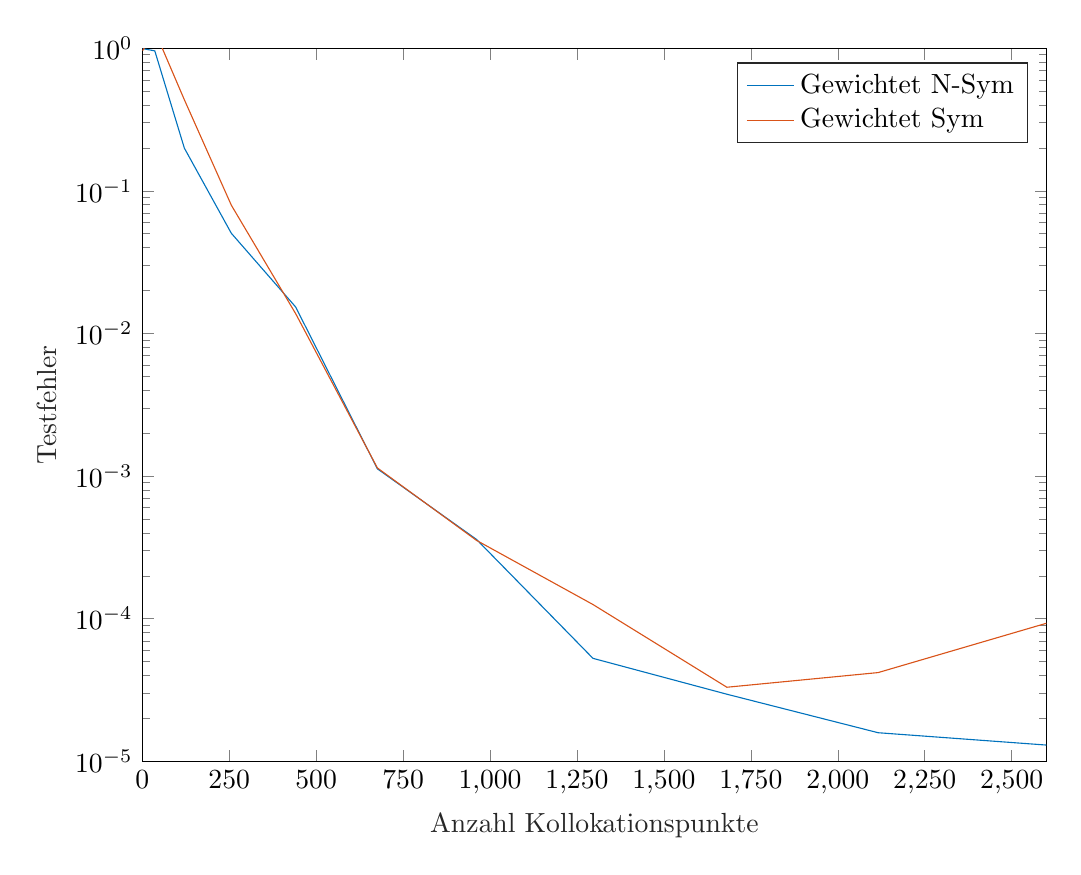
\begin{tikzpicture}

\begin{axis}[%
width=4.521in,
height=3.566in,
at={(0.758in,0.481in)},
scale only axis,
xmin=0,
xmax=2600,
xtick distance={250},
xlabel style={font=\color{white!15!black}},
xlabel={Anzahl Kollokationspunkte},
ymin=1e-05,
ymax=1,
ymode=log,
ylabel style={font=\color{white!15!black}},
ylabel={Testfehler},
axis background/.style={fill=white},
legend style={legend cell align=left, align=left, draw=white!15!black}
]
\addplot [color=mycolor1]
  table[row sep=crcr]{%
1	0.992742646346243\\
36	0.95719159493803\\
121	0.199182045140936\\
256	0.0504075982767586\\
441	0.0153331073518537\\
676	0.00112474393531347\\
961	0.000359925454297583\\
1296	5.27499034438383e-05\\
1681	2.9566939451886e-05\\
2116	1.58778041508822e-05\\
2601	1.30041670055453e-05\\
};
\addlegendentry{Gewichtet N-Sym}

\addplot [color=mycolor2]
  table[row sep=crcr]{%
1	0.960083066620001\\
36	1.32241122108346\\
121	0.4347893064322\\
256	0.0793297977437181\\
441	0.0137708927849018\\
676	0.00114090177907714\\
961	0.000354362614317261\\
1296	0.000125752362927722\\
1681	3.308936362445e-05\\
2116	4.19288442625176e-05\\
2601	9.31282409229528e-05\\
};
\addlegendentry{Gewichtet Sym}

\end{axis}
\end{tikzpicture}%
	}
	\caption{Fehlerplot einer \acs{PDE} in vier Dimensionen}
	\label{fig:4dim}
\end{figure}

Wir erkennen zunächst, dass unsere Verfahren auch in vier Dimensionen funktionieren und gegen die analytische Lösung konvergieren. Wir vergleichen die Ergebnisse hier mit denen aus \ref{fig:andereGewicht}, da die \ac{PDE} und die gewählte Gewichtsfunktion dort vergleichbar sind. Allerdings sehen wir im Vergleich zum zweidimensionalen Fall eine deutlich langsamere Konvergenz, was durch die höhere Dimension auch zu erwarten ist. Demnach benötigen wir in höheren Dimensionen mehr Kollokationspunkte für gute Ergebnisse. Außerdem erreichen wir insgesamt nur einen Fehler von ungefähr $10^{-5}$, was schlechter ist als die Ergebnisse in zwei Dimensionen. Dies ist aber nicht zwangsläufig auf die Dimension zurückzuführen, sondern auch auf die komplizierteren Terme in der Gewichtsfunktion und der rechten Seite der \ac{PDE}, die wir im vierdimensionalen Fall gegeben haben.

\section{Parameterwahl und Kondition}
Wir werden in Abbildung \ref{fig:gamma-grid} zunächst betrachten, wie sich der gewählte Parameter $\gamma$ bei unterschiedlich vielen Kollokationspunkten verhält. Dafür betrachten wir diese aufgrund der gleichmäßigen Verringerung der Abstände auf einem Gitter verteilt. 

\begin{figure}[ht]
\centering
\resizebox {\columnwidth} {!} {
% This file was created by matlab2tikz.
%
%The latest updates can be retrieved from
%  http://www.mathworks.com/matlabcentral/fileexchange/22022-matlab2tikz-matlab2tikz
%where you can also make suggestions and rate matlab2tikz.
%
\definecolor{mycolor1}{rgb}{0.00000,0.44700,0.74100}%
\definecolor{mycolor2}{rgb}{0.85000,0.32500,0.09800}%
\definecolor{mycolor3}{rgb}{0.92900,0.69400,0.12500}%
\definecolor{mycolor4}{rgb}{0.49400,0.18400,0.55600}%
%
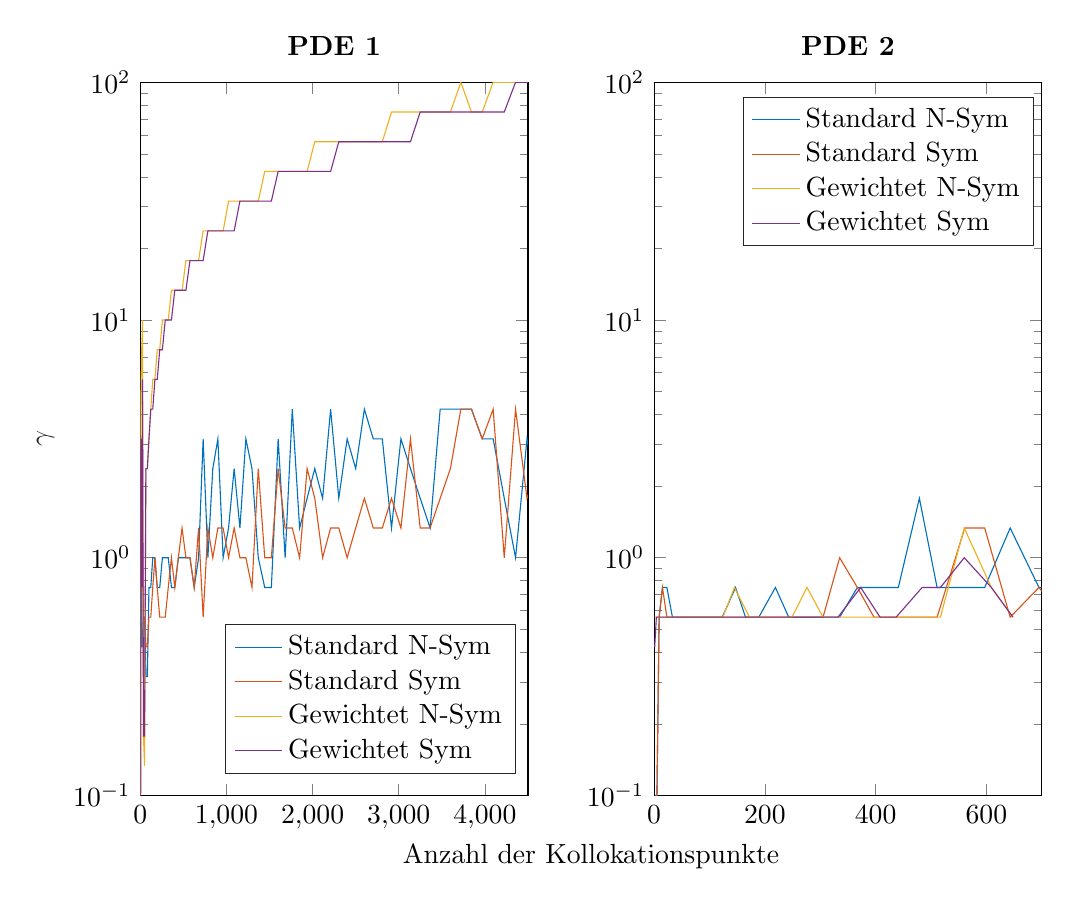
\begin{tikzpicture}

\begin{axis}[%
name = ax1,
width=1.938in,
height=3.566in,
at={(0.758in,0.481in)},
scale only axis,
xmin=0,
xmax=4500,
%xlabel style={font=\color{white!15!black}},
%xlabel={amount of collocation points},
ymode=log,
ymin=1e-01,
ymax=1e+02,
yminorticks=true,
ylabel style={font=\color{white!15!black}},
ylabel={$\gamma$},
axis background/.style={fill=white},
title style={font=\bfseries},
title={\ac{PDE} 1},
legend style={legend cell align=left, align=left, draw=white!15!black},
legend pos = south east
]
\addplot [color=mycolor1]
  table[row sep=crcr]{%
1	0.1\\
4	0.749894209332456\\
9	1\\
16	0.421696503428582\\
25	0.421696503428582\\
36	0.562341325190349\\
49	0.562341325190349\\
64	0.316227766016838\\
81	0.316227766016838\\
100	0.749894209332456\\
121	0.749894209332456\\
144	1\\
169	1\\
196	0.749894209332456\\
225	0.749894209332456\\
256	1\\
289	1\\
324	1\\
361	0.749894209332456\\
400	0.749894209332456\\
441	1\\
484	1\\
529	1\\
576	1\\
625	0.749894209332456\\
676	1\\
729	3.16227766016838\\
784	1\\
841	2.37137370566166\\
900	3.16227766016838\\
961	1\\
1024	1.33352143216332\\
1089	2.37137370566166\\
1156	1.33352143216332\\
1225	3.16227766016838\\
1296	2.37137370566166\\
1369	1\\
1444	0.749894209332456\\
1521	0.749894209332456\\
1600	3.16227766016838\\
1681	1\\
1764	4.21696503428582\\
1849	1.33352143216332\\
1936	1.77827941003892\\
2025	2.37137370566166\\
2116	1.77827941003892\\
2209	4.21696503428582\\
2304	1.77827941003892\\
2401	3.16227766016838\\
2500	2.37137370566166\\
2601	4.21696503428582\\
2704	3.16227766016838\\
2809	3.16227766016838\\
2916	1.33352143216332\\
3025	3.16227766016838\\
3136	2.37137370566166\\
3249	1.77827941003892\\
3364	1.33352143216332\\
3481	4.21696503428582\\
3600	4.21696503428582\\
3721	4.21696503428582\\
3844	4.21696503428582\\
3969	3.16227766016838\\
4096	3.16227766016838\\
4225	1.77827941003892\\
4356	1\\
4489	3.16227766016838\\
4624	1.77827941003892\\
4761	2.37137370566166\\
4900	1\\
5041	3.16227766016838\\
5184	4.21696503428582\\
5329	2.37137370566166\\
5476	1.77827941003892\\
5625	3.16227766016838\\
5776	3.16227766016838\\
5929	4.21696503428582\\
6084	2.37137370566166\\
};
\addlegendentry{Standard N-Sym}

\addplot [color=mycolor2]
  table[row sep=crcr]{%
1	0.1\\
4	0.749894209332456\\
9	0.749894209332456\\
16	1\\
25	1\\
36	0.562341325190349\\
49	0.562341325190349\\
64	0.421696503428582\\
81	0.421696503428582\\
100	0.562341325190349\\
121	0.562341325190349\\
144	0.749894209332456\\
169	1\\
196	0.749894209332456\\
225	0.562341325190349\\
256	0.562341325190349\\
289	0.562341325190349\\
324	0.749894209332456\\
361	1\\
400	0.749894209332456\\
441	1\\
484	1.33352143216332\\
529	1\\
576	1\\
625	0.749894209332456\\
676	1.33352143216332\\
729	0.562341325190349\\
784	1.33352143216332\\
841	1\\
900	1.33352143216332\\
961	1.33352143216332\\
1024	1\\
1089	1.33352143216332\\
1156	1\\
1225	1\\
1296	0.749894209332456\\
1369	2.37137370566166\\
1444	1\\
1521	1\\
1600	2.37137370566166\\
1681	1.33352143216332\\
1764	1.33352143216332\\
1849	1\\
1936	2.37137370566166\\
2025	1.77827941003892\\
2116	1\\
2209	1.33352143216332\\
2304	1.33352143216332\\
2401	1\\
2500	1.33352143216332\\
2601	1.77827941003892\\
2704	1.33352143216332\\
2809	1.33352143216332\\
2916	1.77827941003892\\
3025	1.33352143216332\\
3136	3.16227766016838\\
3249	1.33352143216332\\
3364	1.33352143216332\\
3481	1.77827941003892\\
3600	2.37137370566166\\
3721	4.21696503428582\\
3844	4.21696503428582\\
3969	3.16227766016838\\
4096	4.21696503428582\\
4225	1\\
4356	4.21696503428582\\
4489	1.77827941003892\\
4624	2.37137370566166\\
4761	4.21696503428582\\
4900	4.21696503428582\\
5041	4.21696503428582\\
5184	4.21696503428582\\
5329	4.21696503428582\\
5476	3.16227766016838\\
5625	3.16227766016838\\
5776	3.16227766016838\\
5929	3.16227766016838\\
6084	4.21696503428582\\
};
\addlegendentry{Standard Sym}

\addplot [color=mycolor3]
  table[row sep=crcr]{%
1	0.1\\
4	3.16227766016838\\
9	5.62341325190349\\
16	7.49894209332456\\
25	10\\
36	0.177827941003892\\
49	0.133352143216332\\
64	2.37137370566166\\
81	2.37137370566166\\
100	3.16227766016838\\
121	4.21696503428582\\
144	5.62341325190349\\
169	5.62341325190349\\
196	7.49894209332456\\
225	7.49894209332456\\
256	10\\
289	10\\
324	10\\
361	13.3352143216332\\
400	13.3352143216332\\
441	13.3352143216332\\
484	13.3352143216332\\
529	17.7827941003892\\
576	17.7827941003892\\
625	17.7827941003892\\
676	17.7827941003892\\
729	23.7137370566166\\
784	23.7137370566166\\
841	23.7137370566166\\
900	23.7137370566166\\
961	23.7137370566166\\
1024	31.6227766016838\\
1089	31.6227766016838\\
1156	31.6227766016838\\
1225	31.6227766016838\\
1296	31.6227766016838\\
1369	31.6227766016838\\
1444	42.1696503428582\\
1521	42.1696503428582\\
1600	42.1696503428582\\
1681	42.1696503428582\\
1764	42.1696503428582\\
1849	42.1696503428582\\
1936	42.1696503428582\\
2025	56.2341325190349\\
2116	56.2341325190349\\
2209	56.2341325190349\\
2304	56.2341325190349\\
2401	56.2341325190349\\
2500	56.2341325190349\\
2601	56.2341325190349\\
2704	56.2341325190349\\
2809	56.2341325190349\\
2916	74.9894209332456\\
3025	74.9894209332456\\
3136	74.9894209332456\\
3249	74.9894209332456\\
3364	74.9894209332456\\
3481	74.9894209332456\\
3600	74.9894209332456\\
3721	100\\
3844	74.9894209332456\\
3969	74.9894209332456\\
4096	100\\
4225	100\\
4356	100\\
4489	100\\
4624	100\\
4761	100\\
4900	100\\
5041	100\\
5184	100\\
5329	133.352143216332\\
5476	100\\
5625	133.352143216332\\
5776	133.352143216332\\
5929	133.352143216332\\
6084	133.352143216332\\
};
\addlegendentry{Gewichtet N-Sym}

\addplot [color=mycolor4]
  table[row sep=crcr]{%
1	0.1\\
4	1.77827941003892\\
9	3.16227766016838\\
16	0.749894209332456\\
25	5.62341325190349\\
36	0.177827941003892\\
49	0.177827941003892\\
64	2.37137370566166\\
81	2.37137370566166\\
100	3.16227766016838\\
121	4.21696503428582\\
144	4.21696503428582\\
169	5.62341325190349\\
196	5.62341325190349\\
225	7.49894209332456\\
256	7.49894209332456\\
289	10\\
324	10\\
361	10\\
400	13.3352143216332\\
441	13.3352143216332\\
484	13.3352143216332\\
529	13.3352143216332\\
576	17.7827941003892\\
625	17.7827941003892\\
676	17.7827941003892\\
729	17.7827941003892\\
784	23.7137370566166\\
841	23.7137370566166\\
900	23.7137370566166\\
961	23.7137370566166\\
1024	23.7137370566166\\
1089	23.7137370566166\\
1156	31.6227766016838\\
1225	31.6227766016838\\
1296	31.6227766016838\\
1369	31.6227766016838\\
1444	31.6227766016838\\
1521	31.6227766016838\\
1600	42.1696503428582\\
1681	42.1696503428582\\
1764	42.1696503428582\\
1849	42.1696503428582\\
1936	42.1696503428582\\
2025	42.1696503428582\\
2116	42.1696503428582\\
2209	42.1696503428582\\
2304	56.2341325190349\\
2401	56.2341325190349\\
2500	56.2341325190349\\
2601	56.2341325190349\\
2704	56.2341325190349\\
2809	56.2341325190349\\
2916	56.2341325190349\\
3025	56.2341325190349\\
3136	56.2341325190349\\
3249	74.9894209332456\\
3364	74.9894209332456\\
3481	74.9894209332456\\
3600	74.9894209332456\\
3721	74.9894209332456\\
3844	74.9894209332456\\
3969	74.9894209332456\\
4096	74.9894209332456\\
4225	74.9894209332456\\
4356	100\\
4489	100\\
4624	100\\
};
\addlegendentry{Gewichtet Sym}

\end{axis}

\begin{axis}[%
name = ax2,
width=1.938in,
height=3.566in,
at={(3.327in,0.481in)},
scale only axis,
xmin=0,
xmax=700,
%xlabel style={font=\color{white!15!black}},
%xlabel={amount of collocation points},
ymode=log,
ymin=1e-01,
ymax=1e+02,
yminorticks=true,
%ylabel style={font=\color{white!15!black}},
%ylabel={max. error in derivative/absolute},
axis background/.style={fill=white},
title style={font=\bfseries},
title={\ac{PDE} 2},
legend style={legend cell align=left, align=left, draw=white!15!black}
]
\addplot [color=mycolor1]
  table[row sep=crcr]{%
2	0.1\\
5	0.1\\
9	0.562341325190349\\
15	0.749894209332456\\
23	0.749894209332456\\
33	0.562341325190349\\
45	0.562341325190349\\
55	0.562341325190349\\
71	0.562341325190349\\
89	0.562341325190349\\
101	0.562341325190349\\
123	0.562341325190349\\
147	0.749894209332456\\
165	0.562341325190349\\
189	0.562341325190349\\
219	0.749894209332456\\
243	0.562341325190349\\
269	0.562341325190349\\
305	0.562341325190349\\
335	0.562341325190349\\
367	0.749894209332456\\
397	0.749894209332456\\
441	0.749894209332456\\
479	1.77827941003892\\
511	0.749894209332456\\
561	0.749894209332456\\
597	0.749894209332456\\
643	1.33352143216332\\
695	0.749894209332456\\
737	0.749894209332456\\
};
\addlegendentry{Standard N-Sym}

\addplot [color=mycolor2]
  table[row sep=crcr]{%
2	0.1\\
5	0.1\\
9	0.562341325190349\\
15	0.749894209332456\\
23	0.562341325190349\\
33	0.562341325190349\\
45	0.562341325190349\\
55	0.562341325190349\\
71	0.562341325190349\\
89	0.562341325190349\\
101	0.562341325190349\\
123	0.562341325190349\\
147	0.562341325190349\\
165	0.562341325190349\\
189	0.562341325190349\\
219	0.562341325190349\\
243	0.562341325190349\\
269	0.562341325190349\\
305	0.562341325190349\\
335	1\\
367	0.749894209332456\\
397	0.562341325190349\\
441	0.562341325190349\\
479	0.562341325190349\\
511	0.562341325190349\\
561	1.33352143216332\\
597	1.33352143216332\\
643	0.562341325190349\\
695	0.749894209332456\\
737	0.562341325190349\\
};
\addlegendentry{Standard Sym}

\addplot [color=mycolor3]
  table[row sep=crcr]{%
1	0.562341325190349\\
4	0.562341325190349\\
9	0.562341325190349\\
16	0.562341325190349\\
25	0.562341325190349\\
32	0.562341325190349\\
45	0.562341325190349\\
60	0.562341325190349\\
69	0.562341325190349\\
88	0.562341325190349\\
109	0.562341325190349\\
124	0.562341325190349\\
145	0.749894209332456\\
172	0.562341325190349\\
193	0.562341325190349\\
216	0.562341325190349\\
249	0.562341325190349\\
276	0.749894209332456\\
305	0.562341325190349\\
332	0.562341325190349\\
373	0.562341325190349\\
408	0.562341325190349\\
437	0.562341325190349\\
484	0.562341325190349\\
517	0.562341325190349\\
560	1.33352143216332\\
609	0.749894209332456\\
648	0.562341325190349\\
};
\addlegendentry{Gewichtet N-Sym}

\addplot [color=mycolor4]
  table[row sep=crcr]{%
1	0.421696503428582\\
4	0.562341325190349\\
9	0.562341325190349\\
16	0.562341325190349\\
25	0.562341325190349\\
32	0.562341325190349\\
45	0.562341325190349\\
60	0.562341325190349\\
69	0.562341325190349\\
88	0.562341325190349\\
109	0.562341325190349\\
124	0.562341325190349\\
145	0.562341325190349\\
172	0.562341325190349\\
193	0.562341325190349\\
216	0.562341325190349\\
249	0.562341325190349\\
276	0.562341325190349\\
305	0.562341325190349\\
332	0.562341325190349\\
373	0.749894209332456\\
408	0.562341325190349\\
437	0.562341325190349\\
484	0.749894209332456\\
517	0.749894209332456\\
560	1\\
609	0.749894209332456\\
648	0.562341325190349\\
};
\addlegendentry{Gewichtet Sym}

\end{axis}
\path (ax1.south east) -- (ax2.south west)
  node[midway,below=5mm] {Anzahl der Kollokationspunkte};
\end{tikzpicture}%
}
\caption{Gewählter Parameter $\gamma$}
\label{fig:gamma-grid}
\end{figure}
Wir erkennen, dass die Verfahren, die ihren besten Testfehler in Abbildung \ref{fig:error-grid-both} bereits erreicht haben, ihren $\gamma$-Wert kaum mehr verändern. Es stechen nur die beiden gewichteten Verfahren bei der ersten \ac{PDE} heraus, da sich hier der verwendete Parameter $\gamma$ mit steigender Anzahl der Kollokationspunkte vergrößert. Das waren genau die Verfahren, die ihren Testfehler mit steigender Anzahl der Kollokationspunkte noch verbessert haben. Das größere $\gamma$ resultiert in einem engeren \glqq Hütchen\grqq{} des Kerns, was zu den enger liegenden Kollokationspunkten passt.

In Abbildung \ref{fig:gamma-fehler} ist bei gleichbleibenden Kollokationspunkten der Testfehler beider \acp{PDE} bei unterschiedlichen Parametern $\gamma$ dargestellt.
\begin{figure}[ht]
\centering
\resizebox {\columnwidth} {!} {
% This file was created by matlab2tikz.
%
%The latest updates can be retrieved from
%  http://www.mathworks.com/matlabcentral/fileexchange/22022-matlab2tikz-matlab2tikz
%where you can also make suggestions and rate matlab2tikz.
%
%
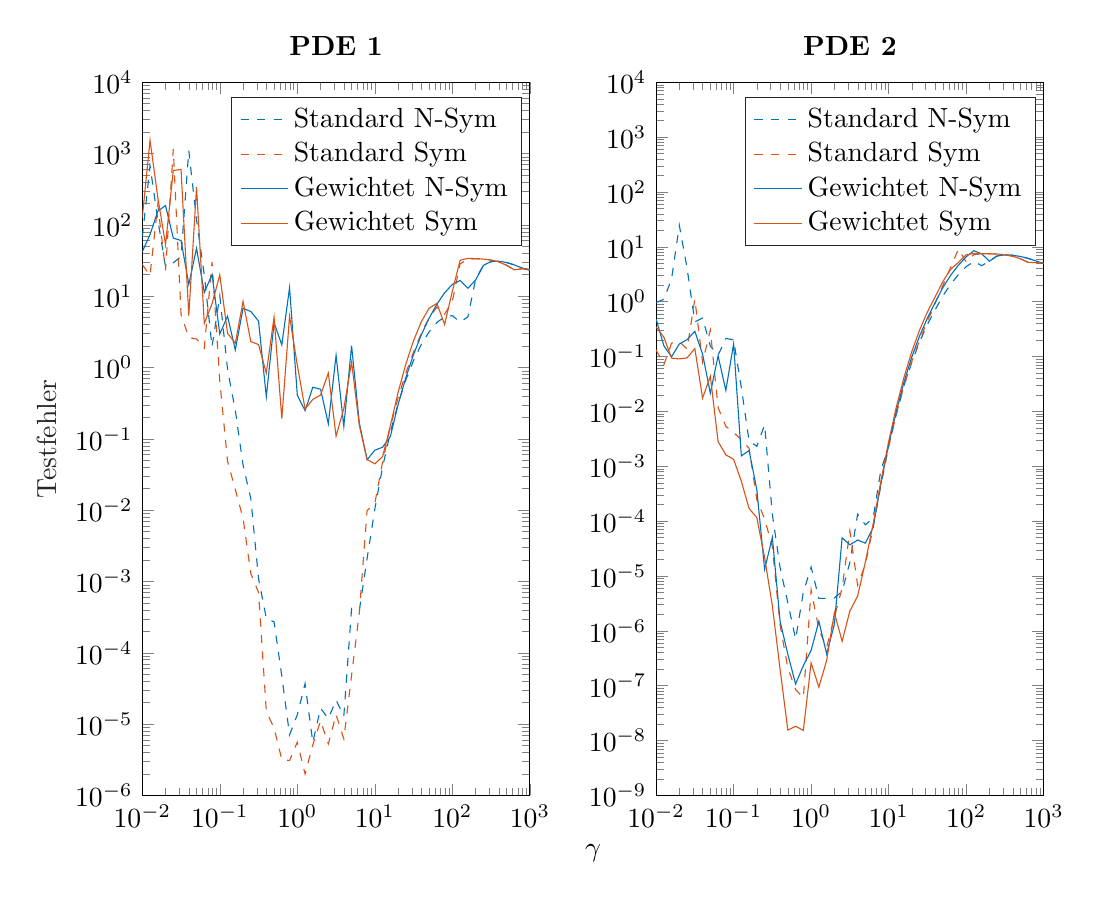
\begin{tikzpicture}

\begin{axis}[%
name = ax1,
width=1.938in,
height=3.566in,
at={(0.758in,0.481in)},
scale only axis,
xmin=1e-02,
xmax=1e+03,
xmode = log,
%xlabel style={font=\color{white!15!black}},
%xlabel={amount of collocation points},
ymode=log,
ymin=1e-06,
ymax=1e+04,
yminorticks=true,
ylabel style={font=\color{white!15!black}},
ylabel={Testfehler},
axis background/.style={fill=white},
title style={font=\bfseries},
title={\ac{PDE} 1},
legend style={legend cell align=left, align=left, draw=white!15!black}
]
\addplot [color=mycolor1, dashed]
  table[row sep=crcr]{%
0.01	66.6303955989106\\
0.0125892541179417	676.260791197821\\
0.0158489319246111	118.658608588145\\
0.0199526231496888	26\\
0.0251188643150958	29.4461318234111\\
0.0316227766016838	35.9788641996389\\
0.0398107170553497	1101.7633489997\\
0.0501187233627272	117.10925979855\\
0.0630957344480193	19.8484686007282\\
0.0794328234724281	1.95863580036112\\
0.1	10.125\\
0.125892541179417	0.946124850728239\\
0.158489319246111	0.250812350728239\\
0.199526231496888	0.04296875\\
0.251188643150958	0.014508730888882\\
0.316227766016838	0.00109454938174736\\
0.398107170553497	0.00030517578125\\
0.501187233627272	0.000271604038371898\\
0.630957344480193	4.6881601728721e-05\\
0.794328234724282	7.08060017640122e-06\\
1	1.35869080644113e-05\\
1.25892541179417	3.69029267552889e-05\\
1.58489319246111	5.55658443346374e-06\\
1.99526231496888	1.67345773114391e-05\\
2.51188643150958	1.19799603082171e-05\\
3.16227766016838	2.17511957076866e-05\\
3.98107170553497	1.29871363254708e-05\\
5.01187233627272	0.00042000588442459\\
6.30957344480193	0.000394845207994265\\
7.94328234724281	0.00210093995097971\\
10	0.0104397307162447\\
12.5892541179417	0.0402529216383858\\
15.8489319246111	0.123404708624564\\
19.9526231496888	0.312229356509478\\
25.1188643150958	0.671819752577322\\
31.6227766016838	1.26229434467618\\
39.8107170553497	2.10963162474283\\
50.1187233627272	3.16683734828455\\
63.0957344480193	4.27466863371273\\
79.4328234724281	5.13798702839628\\
100	5.33908405521724\\
125.892541179417	4.35679288095148\\
158.489319246111	5.12055435395837\\
199.526231496888	17.2180957633892\\
251.188643150958	27.1918609611788\\
316.227766016838	30.6777354211137\\
398.107170553497	30.9442753346661\\
501.187233627272	29.6651276012871\\
630.957344480193	27.4759745463582\\
794.328234724281	24.7981474905116\\
1000	23.1266848774707\\
};
\addlegendentry{Standard N-Sym}

\addplot [color=mycolor2, dashed]
  table[row sep=crcr]{%
0.01	27.8327595884442\\
0.0125892541179417	19.5\\
0.0158489319246111	193.021135800361\\
0.0199526231496888	23\\
0.0251188643150958	1151.15153139927\\
0.0316227766016838	5.61477059891064\\
0.0398107170553497	2.63511419963888\\
0.0501187233627272	2.51171875\\
0.0630957344480193	1.875\\
0.0794328234724281	30.2288641996389\\
0.1	0.645673218450447\\
0.125892541179417	0.0485052497004475\\
0.158489319246111	0.0195353334307526\\
0.199526231496888	0.00769451311825264\\
0.251188643150958	0.00129461956075616\\
0.316227766016838	0.000701904296875\\
0.398107170553497	1.51072288376852e-05\\
0.501187233627272	8.84461351358112e-06\\
0.630957344480193	3.18629988527164e-06\\
0.794328234724282	3.09121660269085e-06\\
1	5.58487425195153e-06\\
1.25892541179417	2.00363288893612e-06\\
1.58489319246111	5.12599945068359e-06\\
1.99526231496888	1.11317407034406e-05\\
2.51188643150958	5.29853948449954e-06\\
3.16227766016838	1.35892857171527e-05\\
3.98107170553497	6.2094009978253e-06\\
5.01187233627272	4.84000862881473e-05\\
6.30957344480193	0.00036899873644991\\
7.94328234724281	0.00988757082288938\\
10	0.0124830961356421\\
12.5892541179417	0.0474470818481496\\
15.8489319246111	0.146785671042835\\
19.9526231496888	0.376544423590541\\
25.1188643150958	0.83449038313913\\
31.6227766016838	1.65831224453839\\
39.8107170553497	3.02502036416536\\
50.1187233627272	5.02415602281089\\
63.0957344480193	7.00481878878612\\
79.4328234724281	5.60604600462379\\
100	8.52862005378399\\
125.892541179417	28.4471209176291\\
158.489319246111	33.0324265416514\\
199.526231496888	33.4565747228332\\
251.188643150958	33.1577018849717\\
316.227766016838	32.1587655469918\\
398.107170553497	30.1578688554254\\
501.187233627272	27.1094230924797\\
630.957344480193	23.3747544078197\\
794.328234724281	24.3001705449842\\
1000	23.8952234665881\\
};
\addlegendentry{Standard Sym}

\addplot [color=mycolor1]
  table[row sep=crcr]{%
0.01	42.1303955989106\\
0.0125892541179417	73.1092597985495\\
0.0158489319246111	155.10925979855\\
0.0199526231496888	186.89074020145\\
0.0251188643150958	65.3413914118553\\
0.0316227766016838	60.3907402014505\\
0.0398107170553497	14.6586085881447\\
0.0501187233627272	46.8907402014505\\
0.0630957344480193	11.3038681765889\\
0.0794328234724281	20.1092597985495\\
0.1	2.95863580036112\\
0.125892541179417	5.24764141185531\\
0.158489319246111	1.76550979854952\\
0.199526231496888	6.77889141185531\\
0.251188643150958	6.10925979854952\\
0.316227766016838	4.47110858814469\\
0.398107170553497	0.390509798549519\\
0.501187233627272	4.26574020145048\\
0.630957344480193	2.07800979854952\\
0.794328234724282	13.1407402014505\\
1	0.408087923549519\\
1.25892541179417	0.249138638950481\\
1.58489319246111	0.529181673549519\\
1.99526231496888	0.496664849355305\\
2.51188643150958	0.162712857700481\\
3.16227766016838	1.47887496707548\\
3.98107170553497	0.149711998865519\\
5.01187233627272	2.02397266285173\\
6.30957344480193	0.166511512719498\\
7.94328234724281	0.0509927014151428\\
10	0.0693719809438873\\
12.5892541179417	0.0763713047024543\\
15.8489319246111	0.10782404158956\\
19.9526231496888	0.302354532533542\\
25.1188643150958	0.726018184274517\\
31.6227766016838	1.52756751559676\\
39.8107170553497	2.8764917472989\\
50.1187233627272	4.9245744810642\\
63.0957344480193	7.73709771190185\\
79.4328234724281	11.1735142904651\\
100	14.664359826692\\
125.892541179417	16.6179505598049\\
158.489319246111	12.933935832866\\
199.526231496888	16.8575105601899\\
251.188643150958	27.05172909274\\
316.227766016838	30.6577437848143\\
398.107170553497	30.959218833163\\
501.187233627272	29.6937134347645\\
630.957344480193	27.5071274704612\\
794.328234724281	24.8256054879479\\
1000	23.1289595304297\\
};
\addlegendentry{Gewichtet N-Sym}

\addplot [color=mycolor2]
  table[row sep=crcr]{%
0.01	125.341391411855\\
0.0125892541179417	1538.89074020145\\
0.0158489319246111	245.10925979855\\
0.0199526231496888	52.9788641996389\\
0.0251188643150958	578.890740201451\\
0.0316227766016838	601.021135800361\\
0.0398107170553497	5.35925979854952\\
0.0501187233627272	338.658608588145\\
0.0630957344480193	4.15860858814469\\
0.0794328234724281	7.84139141185531\\
0.1	19.8907402014505\\
0.125892541179417	3.02107891185531\\
0.158489319246111	2.19263103655575\\
0.199526231496888	8.46639141185531\\
0.251188643150958	2.31238479854952\\
0.316227766016838	2.09754104854952\\
0.398107170553497	0.836052701450481\\
0.501187233627272	5.07824020145048\\
0.630957344480193	0.192953911855306\\
0.794328234724282	5.23449020145048\\
1	1.078125\\
1.25892541179417	0.262335970424519\\
1.58489319246111	0.357415006137981\\
1.99526231496888	0.411750032924519\\
2.51188643150958	0.836922797129069\\
3.16227766016838	0.109244153476848\\
3.98107170553497	0.266343268320475\\
5.01187233627272	1.19135208370577\\
6.30957344480193	0.153956883429966\\
7.94328234724281	0.0514850014675714\\
10	0.0446572157121947\\
12.5892541179417	0.056360834661318\\
15.8489319246111	0.152960877048847\\
19.9526231496888	0.449559352819401\\
25.1188643150958	1.1197933220361\\
31.6227766016838	2.3925868953584\\
39.8107170553497	4.3953958302469\\
50.1187233627272	6.77749764088432\\
63.0957344480193	7.93900980451617\\
79.4328234724281	4.01832832785593\\
100	11.7634919224365\\
125.892541179417	31.9407308758371\\
158.489319246111	34.0222600467237\\
199.526231496888	33.6629576719211\\
251.188643150958	33.18628969565\\
316.227766016838	32.189069505006\\
398.107170553497	30.1933282680573\\
501.187233627272	27.1418954499323\\
630.957344480193	23.3963582051801\\
794.328234724281	24.3248285875366\\
1000	23.9167477805245\\
};
\addlegendentry{Gewichtet Sym}

\end{axis}

\begin{axis}[%
name = ax2,
width=1.938in,
height=3.566in,
at={(3.327in,0.481in)},
scale only axis,
xmin=1e-02,
xmax=1e+03,
xmode = log,
%xlabel style={font=\color{white!15!black}},
%xlabel={amount of collocation points},
ymode=log,
ymin=1e-09,
ymax=1e+04,
yminorticks=true,
%ylabel style={font=\color{white!15!black}},
%ylabel={max. error in derivative/absolute},
axis background/.style={fill=white},
title style={font=\bfseries},
title={\ac{PDE} 2},
legend style={legend cell align=left, align=left, draw=white!15!black}
]
\addplot [color=mycolor1, dashed]
  table[row sep=crcr]{%
0.01	0.964821685467266\\
0.0125892541179417	1.10720830844984\\
0.0158489319246111	2.59939580844984\\
0.0199526231496888	24.6671895174392\\
0.0251188643150958	4.06402201112432\\
0.0316227766016838	0.429688320991292\\
0.0398107170553497	0.504736303626247\\
0.0501187233627272	0.155611485550534\\
0.0630957344480193	0.106107264449466\\
0.0794328234724281	0.214865814532734\\
0.1	0.201193939532734\\
0.125892541179417	0.0271200012652448\\
0.158489319246111	0.00286986207921669\\
0.199526231496888	0.00232015692879184\\
0.251188643150958	0.00569801991689967\\
0.316227766016838	0.000133010598991734\\
0.398107170553497	1.41724317215264e-05\\
0.501187233627272	3.24625029346493e-06\\
0.630957344480193	7.11168742728585e-07\\
0.794328234724282	5.08640737839627e-06\\
1	1.45990509753946e-05\\
1.25892541179417	3.91491839940583e-06\\
1.58489319246111	3.90819122736419e-06\\
1.99526231496888	3.98699121734181e-06\\
2.51188643150958	5.23439457361663e-06\\
3.16227766016838	1.78186808555969e-05\\
3.98107170553497	0.000133927549815727\\
5.01187233627272	8.5766996837211e-05\\
6.30957344480193	0.000114101554847312\\
7.94328234724281	0.00085166433045919\\
10	0.00231462988971171\\
12.5892541179417	0.00897291958766427\\
15.8489319246111	0.0299979436847351\\
19.9526231496888	0.0794617232287892\\
25.1188643150958	0.186689695601388\\
31.6227766016838	0.384956760930988\\
39.8107170553497	0.714270978549156\\
50.1187233627272	1.284720840902\\
63.0957344480193	2.08307564768658\\
79.4328234724281	3.11538985598953\\
100	4.34539205274069\\
125.892541179417	5.4202809053786\\
158.489319246111	4.5424916539543\\
199.526231496888	5.52407794178772\\
251.188643150958	6.84496156100696\\
316.227766016838	7.13828697017756\\
398.107170553497	7.02534118631451\\
501.187233627272	6.67621459531028\\
630.957344480193	6.16068281640786\\
794.328234724281	5.54948301832508\\
1000	4.92775401684893\\
};
\addlegendentry{Standard N-Sym}

\addplot [color=mycolor2, dashed]
  table[row sep=crcr]{%
0.01	0.132977901005511\\
0.0125892541179417	0.0705872146998375\\
0.0158489319246111	0.176004998734755\\
0.0199526231496888	0.187522064532734\\
0.0251188643150958	0.137567284046084\\
0.0316227766016838	1.11305702039673\\
0.0398107170553497	0.0788879959498375\\
0.0501187233627272	0.304048985550534\\
0.0630957344480193	0.0117759173743222\\
0.0794328234724281	0.00534902921726649\\
0.1	0.00413047960326507\\
0.125892541179417	0.00304874998078564\\
0.158489319246111	0.00213617397203747\\
0.199526231496888	0.000246590131670832\\
0.251188643150958	0.000109802569842887\\
0.316227766016838	3.42757786780945e-05\\
0.398107170553497	1.2690119112202e-06\\
0.501187233627272	2.0965153629815e-07\\
0.630957344480193	8.5210770883748e-08\\
0.794328234724282	6.04320103403388e-08\\
1	5.61365077550446e-06\\
1.25892541179417	1.06206943933929e-06\\
1.58489319246111	4.97687959122306e-07\\
1.99526231496888	1.78218970353639e-06\\
2.51188643150958	6.05395843927825e-06\\
3.16227766016838	6.68052692180399e-05\\
3.98107170553497	6.80395241642318e-06\\
5.01187233627272	1.64537798827413e-05\\
6.30957344480193	7.65627432743332e-05\\
7.94328234724281	0.000446902281184658\\
10	0.00226233031104212\\
12.5892541179417	0.00914366128829297\\
15.8489319246111	0.0300878874347258\\
19.9526231496888	0.0825752975738595\\
25.1188643150958	0.199263002957121\\
31.6227766016838	0.443403353550366\\
39.8107170553497	0.934547501783311\\
50.1187233627272	1.97718047719838\\
63.0957344480193	4.24013905208324\\
79.4328234724281	9.08510268633271\\
100	5.34001884188209\\
125.892541179417	7.21447854239523\\
158.489319246111	7.47157836687895\\
199.526231496888	7.4798229105139\\
251.188643150958	7.40257478189823\\
316.227766016838	7.18201021630443\\
398.107170553497	6.73878609022669\\
501.187233627272	6.05853926553302\\
630.957344480193	5.22183586973772\\
794.328234724281	5.16671400503762\\
1000	5.08347610394243\\
};
\addlegendentry{Standard Sym}

\addplot [color=mycolor1]
  table[row sep=crcr]{%
0.01	0.485829720708796\\
0.0125892541179417	0.157539208874419\\
0.0158489319246111	0.0994439739944888\\
0.0199526231496888	0.169679894281604\\
0.0251188643150958	0.2038181371044\\
0.0316227766016838	0.288838270396735\\
0.0398107170553497	0.110689610550534\\
0.0501187233627272	0.0215064395327335\\
0.0630957344480193	0.103209374041966\\
0.0794328234724281	0.0241495299847552\\
0.1	0.169899810467266\\
0.125892541179417	0.00154627079649483\\
0.158489319246111	0.0019430019587956\\
0.199526231496888	0.000370508396354108\\
0.251188643150958	1.32419795475514e-05\\
0.316227766016838	5.06774217940986e-05\\
0.398107170553497	1.49240929747663e-06\\
0.501187233627272	3.73618322946356e-07\\
0.630957344480193	1.07684569705668e-07\\
0.794328234724282	2.33400261950845e-07\\
1	4.39933104168233e-07\\
1.25892541179417	1.50165369455779e-06\\
1.58489319246111	3.81272637295371e-07\\
1.99526231496888	1.3153891796347e-06\\
2.51188643150958	4.9699459576058e-05\\
3.16227766016838	3.70923537975076e-05\\
3.98107170553497	4.53259687656637e-05\\
5.01187233627272	3.97324206319882e-05\\
6.30957344480193	7.68679185984555e-05\\
7.94328234724281	0.000475167902310114\\
10	0.00249781904288821\\
12.5892541179417	0.0103338136620877\\
15.8489319246111	0.0351260542964928\\
19.9526231496888	0.0994010304086418\\
25.1188643150958	0.238838978628819\\
31.6227766016838	0.501238150264756\\
39.8107170553497	0.96465661778164\\
50.1187233627272	1.81799316379898\\
63.0957344480193	3.03383393543067\\
79.4328234724281	4.62665097482194\\
100	6.5836872347929\\
125.892541179417	8.49945718456336\\
158.489319246111	7.47017674075046\\
199.526231496888	5.48339012640114\\
251.188643150958	6.8333101398448\\
316.227766016838	7.1375119996925\\
398.107170553497	7.02790115265888\\
501.187233627272	6.67993562716014\\
630.957344480193	6.16452931278068\\
794.328234724281	5.55283533069821\\
1000	4.93025760760482\\
};
\addlegendentry{Gewichtet N-Sym}

\addplot [color=mycolor2]
  table[row sep=crcr]{%
0.01	0.347584520337449\\
0.0125892541179417	0.226561679008708\\
0.0158489319246111	0.093821729662551\\
0.0199526231496888	0.090748582837449\\
0.0251188643150958	0.0948730713737533\\
0.0316227766016838	0.139961083874419\\
0.0398107170553497	0.017516014666966\\
0.0501187233627272	0.0437215637652448\\
0.0630957344480193	0.00283205574875328\\
0.0794328234724281	0.0016124518186108\\
0.1	0.00134578126921436\\
0.125892541179417	0.000531611943011212\\
0.158489319246111	0.000170110999293593\\
0.199526231496888	0.000115598681105666\\
0.251188643150958	2.16174978976968e-05\\
0.316227766016838	2.8718371158365e-06\\
0.398107170553497	1.97802090096122e-07\\
0.501187233627272	1.55323743866731e-08\\
0.630957344480193	1.82647472146691e-08\\
0.794328234724282	1.53543641689957e-08\\
1	2.60699654919261e-07\\
1.25892541179417	9.41675370458306e-08\\
1.58489319246111	2.89071702408439e-07\\
1.99526231496888	2.14426627104247e-06\\
2.51188643150958	6.48770130229348e-07\\
3.16227766016838	2.30384676064288e-06\\
3.98107170553497	4.31450352367246e-06\\
5.01187233627272	1.80593800013784e-05\\
6.30957344480193	8.82278316497453e-05\\
7.94328234724281	0.000533089995584934\\
10	0.00282515028884217\\
12.5892541179417	0.0121632213138552\\
15.8489319246111	0.0427533137421781\\
19.9526231496888	0.124639654538644\\
25.1188643150958	0.307134625387552\\
31.6227766016838	0.649027500143529\\
39.8107170553497	1.22364106297731\\
50.1187233627272	2.3388417822451\\
63.0957344480193	3.90796802433792\\
79.4328234724281	5.18844577156421\\
100	7.17029515957315\\
125.892541179417	7.56806552550978\\
158.489319246111	7.49416774484293\\
199.526231496888	7.48442984540263\\
251.188643150958	7.40547337867075\\
316.227766016838	7.18584956805767\\
398.107170553497	6.74339339496247\\
501.187233627272	6.06262092467039\\
630.957344480193	5.22426286979371\\
794.328234724281	5.16752214762745\\
1000	5.08495257021128\\
};
\addlegendentry{Gewichtet Sym}

\end{axis}
\path (ax1.south east) -- (ax2.south west)
  node[midway,below=5mm] {$\gamma$};
\end{tikzpicture}%
}
\caption{Fehler bei verschiedenen Parametern $\gamma$}
\label{fig:gamma-fehler}
\end{figure}
Daraus erkennt man, dass der Testfehler groß ist, wenn $\gamma$ entweder zu klein oder zu groß ist. Ist $\gamma$ zu groß, haben wir zu kleine \glqq Hütchen\grqq , so können diese die \ac{PDE} nur sehr lokal lösen. Der große Testfehler für zu kleines $\gamma$ lässt sich besser erklären, wenn man noch die Kondition hinzunimmt. Diese ist in Abbildung \ref{fig:kondition} dargestellt.
\begin{figure}[ht]
\centering
\resizebox {\columnwidth} {!} {
% This file was created by matlab2tikz.
%
%The latest updates can be retrieved from
%  http://www.mathworks.com/matlabcentral/fileexchange/22022-matlab2tikz-matlab2tikz
%where you can also make suggestions and rate matlab2tikz.
%
%
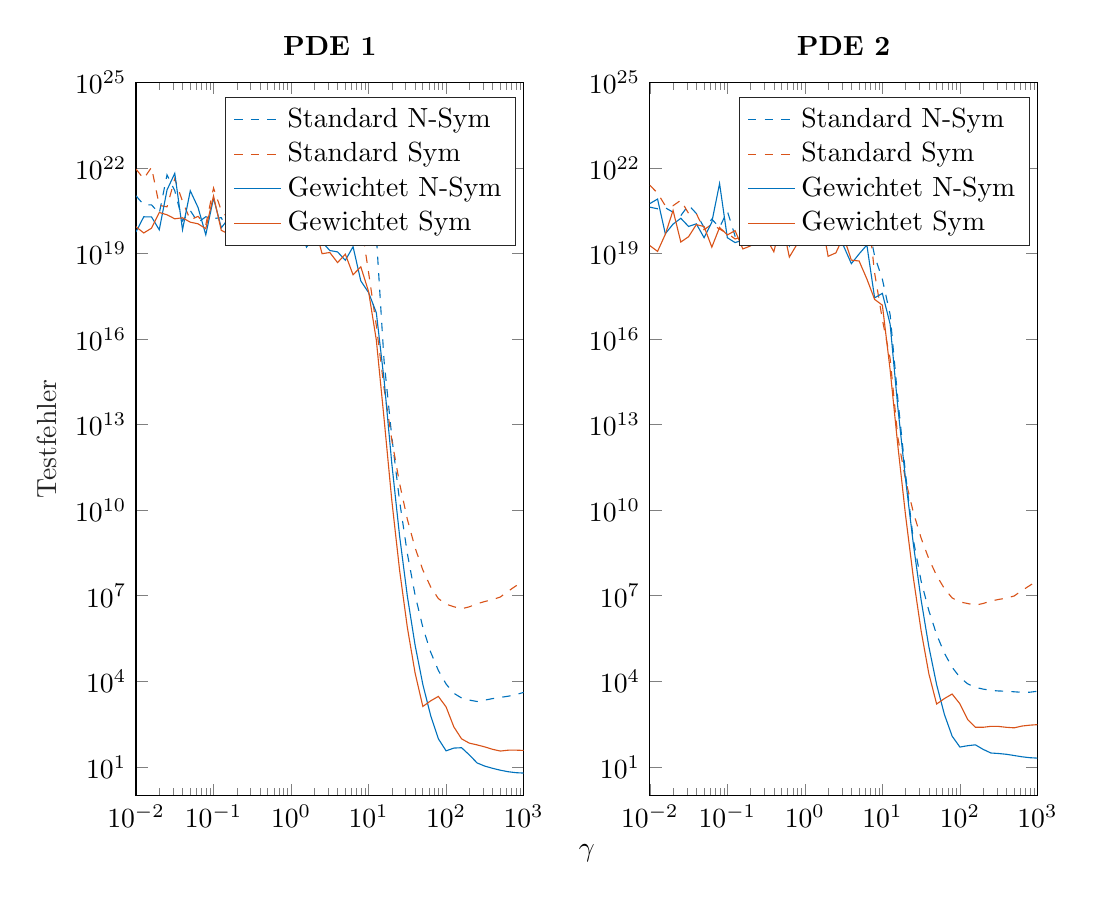
\begin{tikzpicture}

\begin{axis}[%
name = ax1,
width=1.938in,
height=3.566in,
at={(0.758in,0.481in)},
scale only axis,
xmin=1e-02,
xmax=1e+03,
xmode = log,
%xlabel style={font=\color{white!15!black}},
%xlabel={amount of collocation points},
ymode=log,
ymin=1,
ymax=1e+25,
yminorticks=true,
ylabel style={font=\color{white!15!black}},
ylabel={Testfehler},
axis background/.style={fill=white},
title style={font=\bfseries},
title={\ac{PDE} 1},
legend style={legend cell align=left, align=left, draw=white!15!black}
]
\addplot [color=mycolor1, dashed]
  table[row sep=crcr]{%
0.01	1.04865845929151e+21\\
0.0125892541179417	5.04230595583907e+20\\
0.0158489319246111	5.05000936321188e+20\\
0.0199526231496888	2.52379450039901e+20\\
0.0251188643150958	5.69115837827846e+21\\
0.0316227766016838	1.58114985472277e+21\\
0.0398107170553497	1.3866700231325e+20\\
0.0501187233627272	3.1926578893928e+20\\
0.0630957344480193	1.21662006170304e+20\\
0.0794328234724281	1.93064936798815e+20\\
0.1	1.67919898464997e+20\\
0.125892541179417	1.79085011046747e+20\\
0.158489319246111	4.66214030646914e+19\\
0.199526231496888	5.8589789368839e+19\\
0.251188643150958	1.22559930419028e+20\\
0.316227766016838	4.44193820800609e+19\\
0.398107170553497	9.52229693168543e+19\\
0.501187233627272	1.84619565483567e+20\\
0.630957344480193	1.64819860870167e+20\\
0.794328234724282	6.56599217712673e+19\\
1	5.22875037343918e+19\\
1.25892541179417	8.24424054780846e+19\\
1.58489319246111	1.53643608873934e+20\\
1.99526231496888	5.24023948674021e+19\\
2.51188643150958	8.14375805317896e+19\\
3.16227766016838	9.29607986870886e+20\\
3.98107170553497	2.59356593231286e+22\\
5.01187233627272	4.87576760127071e+19\\
6.30957344480193	1.13514598630617e+20\\
7.94328234724281	3.44598704741416e+19\\
10	1.5685808311729e+20\\
12.5892541179417	4.24146428486416e+19\\
15.8489319246111	1.69315548282916e+15\\
19.9526231496888	3638501624770.68\\
25.1188643150958	20933397170.84\\
31.6227766016838	305284229.945374\\
39.8107170553497	10599219.0341428\\
50.1187233627272	783490.776809662\\
63.0957344480193	107571.380311838\\
79.4328234724281	24206.3148313729\\
100	8078.758022606\\
125.892541179417	3816.26585728688\\
158.489319246111	2612.41146050071\\
199.526231496888	2204.18765240733\\
251.188643150958	1967.8212171274\\
316.227766016838	2200.11388781108\\
398.107170553497	2489.65033621437\\
501.187233627272	2735.33013284363\\
630.957344480193	3010.97886053831\\
794.328234724281	3432.00043066879\\
1000	4098.65886645448\\
};
\addlegendentry{Standard N-Sym}

\addplot [color=mycolor2, dashed]
  table[row sep=crcr]{%
0.01	8.99814841888007e+21\\
0.0125892541179417	4.14171394126264e+21\\
0.0158489319246111	1.04512976375315e+22\\
0.0199526231496888	4.83302040494442e+20\\
0.0251188643150958	4.29025471343112e+20\\
0.0316227766016838	4.13754956667125e+21\\
0.0398107170553497	6.66456343847981e+20\\
0.0501187233627272	1.50548537288082e+20\\
0.0630957344480193	1.98861562407094e+20\\
0.0794328234724281	1.00055548327619e+20\\
0.1	1.96110905638352e+21\\
0.125892541179417	3.18910971136302e+20\\
0.158489319246111	1.57969864750628e+20\\
0.199526231496888	7.53931374708785e+19\\
0.251188643150958	3.13259497457297e+20\\
0.316227766016838	4.45922724410824e+19\\
0.398107170553497	2.73084071239116e+20\\
0.501187233627272	1.10605157816781e+20\\
0.630957344480193	2.30261846307151e+20\\
0.794328234724282	1.80556470807567e+20\\
1	2.07489884231578e+20\\
1.25892541179417	6.708071219636e+20\\
1.58489319246111	2.61326041724027e+20\\
1.99526231496888	1.07857877807081e+21\\
2.51188643150958	3.71006068603151e+20\\
3.16227766016838	7.48462051352863e+20\\
3.98107170553497	4.93368748492838e+21\\
5.01187233627272	2.0712611805303e+22\\
6.30957344480193	8.27799588778274e+21\\
7.94328234724281	1.35526937603996e+20\\
10	2.15822668435017e+18\\
12.5892541179417	2.95462530541834e+16\\
15.8489319246111	187194919440375\\
19.9526231496888	2864454075244.34\\
25.1188643150958	86932454007.179\\
31.6227766016838	4836314042.95356\\
39.8107170553497	480389206.772984\\
50.1187233627272	80091039.6135282\\
63.0957344480193	20692201.1845295\\
79.4328234724281	7991978.57500259\\
100	5062798.13171404\\
125.892541179417	4121603.12552517\\
158.489319246111	3507641.80941091\\
199.526231496888	4107204.37130167\\
251.188643150958	5243118.3308861\\
316.227766016838	6302556.39697341\\
398.107170553497	7334174.31026934\\
501.187233627272	9050166.47503784\\
630.957344480193	14444549.4987741\\
794.328234724281	22091632.4835909\\
1000	33446246.473388\\
};
\addlegendentry{Standard Sym}

\addplot [color=mycolor1]
  table[row sep=crcr]{%
0.01	5.67290383545114e+19\\
0.0125892541179417	1.92519035211396e+20\\
0.0158489319246111	1.90050649649849e+20\\
0.0199526231496888	6.7363304679862e+19\\
0.0251188643150958	1.67601398805175e+21\\
0.0316227766016838	6.41812200404691e+21\\
0.0398107170553497	6.78701736103643e+19\\
0.0501187233627272	1.56871937012032e+21\\
0.0630957344480193	4.09177459220934e+20\\
0.0794328234724281	4.5009233010322e+19\\
0.1	8.6852973212117e+20\\
0.125892541179417	7.91714615609991e+19\\
0.158489319246111	1.75696737692271e+20\\
0.199526231496888	4.86063981631839e+19\\
0.251188643150958	2.03703167607491e+20\\
0.316227766016838	7.80626942174749e+19\\
0.398107170553497	9.22740504075686e+19\\
0.501187233627272	1.14978528900945e+20\\
0.630957344480193	3.37027387706651e+19\\
0.794328234724282	1.69001024940748e+20\\
1	5.83396104195637e+19\\
1.25892541179417	6.37845103331407e+19\\
1.58489319246111	1.66014476919381e+19\\
1.99526231496888	4.05507596109228e+19\\
2.51188643150958	2.54241169803801e+19\\
3.16227766016838	1.26353671839003e+19\\
3.98107170553497	1.13287753993839e+19\\
5.01187233627272	5.75873489292593e+18\\
6.30957344480193	1.71479105135187e+19\\
7.94328234724281	1.08341091951405e+18\\
10	4.2765548789834e+17\\
12.5892541179417	8.35319183343512e+16\\
15.8489319246111	373968890395804\\
19.9526231496888	423973008825.204\\
25.1188643150958	1260081232.5872\\
31.6227766016838	9819966.90102297\\
39.8107170553497	186851.510801173\\
50.1187233627272	7811.32275072332\\
63.0957344480193	645.510663337884\\
79.4328234724281	97.5366941645454\\
100	36.6761425462848\\
125.892541179417	45.8179896593759\\
158.489319246111	47.2253324328988\\
199.526231496888	26.378823925423\\
251.188643150958	13.814535961738\\
316.227766016838	10.675570494072\\
398.107170553497	8.9483494454329\\
501.187233627272	7.68748216400347\\
630.957344480193	6.8043306738145\\
794.328234724281	6.29740590219392\\
1000	6.09434620304036\\
};
\addlegendentry{Gewichtet N-Sym}

\addplot [color=mycolor2]
  table[row sep=crcr]{%
0.01	8.5946692978416e+19\\
0.0125892541179417	5.21271294643067e+19\\
0.0158489319246111	7.67377862876893e+19\\
0.0199526231496888	2.72718764506913e+20\\
0.0251188643150958	2.26322349739999e+20\\
0.0316227766016838	1.6367092083517e+20\\
0.0398107170553497	1.77372892765137e+20\\
0.0501187233627272	1.24707826878907e+20\\
0.0630957344480193	1.09251731451873e+20\\
0.0794328234724281	7.35586072378269e+19\\
0.1	1.03004446108577e+21\\
0.125892541179417	6.42171168319296e+19\\
0.158489319246111	4.71734617293966e+19\\
0.199526231496888	7.55812991427095e+19\\
0.251188643150958	5.1756422104934e+19\\
0.316227766016838	9.73673484423001e+19\\
0.398107170553497	3.43720736350741e+19\\
0.501187233627272	3.65834616863515e+19\\
0.630957344480193	3.42700705426551e+19\\
0.794328234724282	2.62139485012807e+19\\
1	2.47086255086544e+20\\
1.25892541179417	3.47956438870528e+19\\
1.58489319246111	7.18805833770636e+19\\
1.99526231496888	1.06069639533376e+20\\
2.51188643150958	9.78241364984761e+18\\
3.16227766016838	1.077536643707e+19\\
3.98107170553497	4.77918505671731e+18\\
5.01187233627272	9.40928340273191e+18\\
6.30957344480193	1.78631061401805e+18\\
7.94328234724281	3.3861394022583e+18\\
10	4.61330117863578e+17\\
12.5892541179417	9.20453823748179e+15\\
15.8489319246111	15939750835764.1\\
19.9526231496888	21636785122.4624\\
25.1188643150958	79190854.1748787\\
31.6227766016838	782038.908323403\\
39.8107170553497	19662.2174671564\\
50.1187233627272	1319.72342926369\\
63.0957344480193	2064.62431861147\\
79.4328234724281	2968.18130327614\\
100	1271.69311127071\\
125.892541179417	252.900160360747\\
158.489319246111	96.3963669753044\\
199.526231496888	68.290649584935\\
251.188643150958	59.2856581026384\\
316.227766016838	50.3365335941792\\
398.107170553497	41.4467432135912\\
501.187233627272	36.0381195809866\\
630.957344480193	38.6404814769115\\
794.328234724281	38.7682989348978\\
1000	38.0006947392212\\
};
\addlegendentry{Gewichtet Sym}

\end{axis}

\begin{axis}[%
name = ax2,
width=1.938in,
height=3.566in,
at={(3.327in,0.481in)},
scale only axis,
xmin=1e-02,
xmax=1e+03,
xmode = log,
%xlabel style={font=\color{white!15!black}},
%xlabel={amount of collocation points},
ymode=log,
ymin=1,
ymax=1e+25,
yminorticks=true,
%ylabel style={font=\color{white!15!black}},
%ylabel={max. error in derivative/absolute},
axis background/.style={fill=white},
title style={font=\bfseries},
title={\ac{PDE} 2},
legend style={legend cell align=left, align=left, draw=white!15!black}
]
\addplot [color=mycolor1, dashed]
  table[row sep=crcr]{%
0.01	4.18792139497458e+20\\
0.0125892541179417	3.67110746509815e+20\\
0.0158489319246111	3.98452016223845e+20\\
0.0199526231496888	2.79064257377878e+20\\
0.0251188643150958	2.1192527647668e+20\\
0.0316227766016838	4.95968659708188e+20\\
0.0398107170553497	2.51701173521569e+20\\
0.0501187233627272	8.08068505838715e+19\\
0.0630957344480193	1.58981520599537e+20\\
0.0794328234724281	8.10675951872382e+19\\
0.1	3.04736086766127e+20\\
0.125892541179417	4.04111831805828e+19\\
0.158489319246111	6.78240675397546e+19\\
0.199526231496888	5.94197082871071e+20\\
0.251188643150958	1.43713532597337e+20\\
0.316227766016838	2.49431547592946e+20\\
0.398107170553497	1.22429113423098e+20\\
0.501187233627272	2.88755031896523e+20\\
0.630957344480193	4.4824713988683e+19\\
0.794328234724282	2.22993116637358e+20\\
1	8.45184530767106e+19\\
1.25892541179417	3.19450525614967e+19\\
1.58489319246111	6.15489829339109e+20\\
1.99526231496888	3.29779870019693e+20\\
2.51188643150958	9.2350166511668e+19\\
3.16227766016838	5.33780464701819e+20\\
3.98107170553497	4.5882504100542e+19\\
5.01187233627272	1.17800406100657e+20\\
6.30957344480193	1.82091189169772e+20\\
7.94328234724281	8.18257148634149e+18\\
10	1.24313042533272e+18\\
12.5892541179417	7.15838107222336e+16\\
15.8489319246111	74911537826263\\
19.9526231496888	175697176468.65\\
25.1188643150958	894121568.395728\\
31.6227766016838	32533613.7809095\\
39.8107170553497	2979124.59245621\\
50.1187233627272	437659.088843961\\
63.0957344480193	97406.2691943202\\
79.4328234724281	31172.4416009502\\
100	13835.9478310216\\
125.892541179417	8189.55950268068\\
158.489319246111	6176.45841190691\\
199.526231496888	5348.8225891268\\
251.188643150958	4854.46506114488\\
316.227766016838	4593.71619399115\\
398.107170553497	4532.34750250767\\
501.187233627272	4308.53031175343\\
630.957344480193	4128.29148767565\\
794.328234724281	4158.74894436644\\
1000	4498.1866789134\\
};
\addlegendentry{Standard N-Sym}

\addplot [color=mycolor2, dashed]
  table[row sep=crcr]{%
0.01	2.46259725397663e+21\\
0.0125892541179417	1.30120628912483e+21\\
0.0158489319246111	4.67839956258406e+20\\
0.0199526231496888	4.71075349425746e+20\\
0.0251188643150958	7.30260106814315e+20\\
0.0316227766016838	2.54463866069551e+20\\
0.0398107170553497	2.50803803548956e+20\\
0.0501187233627272	6.78418342589397e+19\\
0.0630957344480193	1.05428700956687e+20\\
0.0794328234724281	7.12387687325491e+19\\
0.1	5.09831718328189e+19\\
0.125892541179417	3.21089976935033e+19\\
0.158489319246111	3.94519596767924e+19\\
0.199526231496888	2.16463701446189e+20\\
0.251188643150958	8.85251981498958e+19\\
0.316227766016838	4.25169474481485e+20\\
0.398107170553497	8.63472278046989e+19\\
0.501187233627272	4.06235420576839e+19\\
0.630957344480193	3.26437723343207e+19\\
0.794328234724282	1.2972444755997e+20\\
1	1.30656613674207e+20\\
1.25892541179417	3.35469940696103e+20\\
1.58489319246111	2.95990602810424e+20\\
1.99526231496888	3.55127422063768e+20\\
2.51188643150958	4.83374462122735e+21\\
3.16227766016838	1.04734826071877e+21\\
3.98107170553497	5.54499181878539e+21\\
5.01187233627272	1.22574029808681e+22\\
6.30957344480193	6.27377931452376e+20\\
7.94328234724281	2.05729179818083e+18\\
10	4.80243715399579e+16\\
12.5892541179417	2.05182232993884e+15\\
15.8489319246111	3453838461799.66\\
19.9526231496888	112236340864.678\\
25.1188643150958	8303851618.06995\\
31.6227766016838	1049595263.56943\\
39.8107170553497	196071739.929222\\
50.1187233627272	51047748.0742787\\
63.0957344480193	17854429.1871512\\
79.4328234724281	8410772.72185044\\
100	6074162.07417215\\
125.892541179417	5356064.56994469\\
158.489319246111	4684008.65701961\\
199.526231496888	5371156.35793379\\
251.188643150958	6533620.93549852\\
316.227766016838	7435300.00019652\\
398.107170553497	8255409.74348304\\
501.187233627272	9826264.0463129\\
630.957344480193	15232456.107076\\
794.328234724281	22737188.1918416\\
1000	33807354.0719527\\
};
\addlegendentry{Standard Sym}

\addplot [color=mycolor1]
  table[row sep=crcr]{%
0.01	5.58285531771304e+20\\
0.0125892541179417	8.03834872234642e+20\\
0.0158489319246111	4.88723448412943e+19\\
0.0199526231496888	1.06582588243275e+20\\
0.0251188643150958	1.70867574344126e+20\\
0.0316227766016838	8.80448410366788e+19\\
0.0398107170553497	1.09155994721116e+20\\
0.0501187233627272	3.56535134718306e+19\\
0.0630957344480193	1.25154166685929e+20\\
0.0794328234724281	2.82154403843102e+21\\
0.1	3.55991856860406e+19\\
0.125892541179417	2.40069324011765e+19\\
0.158489319246111	2.91394568820761e+19\\
0.199526231496888	8.41483436316887e+19\\
0.251188643150958	1.38769866798688e+20\\
0.316227766016838	6.26095227898404e+19\\
0.398107170553497	9.76121370542415e+19\\
0.501187233627272	1.07141066885896e+20\\
0.630957344480193	1.90920982283854e+19\\
0.794328234724282	1.17649554792725e+21\\
1	1.23231867474705e+20\\
1.25892541179417	1.04856584702239e+20\\
1.58489319246111	6.19799360380503e+19\\
1.99526231496888	2.09769186018637e+19\\
2.51188643150958	5.47782359444808e+19\\
3.16227766016838	1.81114156120519e+19\\
3.98107170553497	4.3815610774082e+18\\
5.01187233627272	9.60936822595577e+18\\
6.30957344480193	1.97516358400896e+19\\
7.94328234724281	2.77105297652695e+17\\
10	3.98497193520408e+17\\
12.5892541179417	3.34344194066479e+16\\
15.8489319246111	38877740369868.2\\
19.9526231496888	115775316582.229\\
25.1188643150958	635347756.433704\\
31.6227766016838	7049759.02289853\\
39.8107170553497	163097.674434608\\
50.1187233627272	7653.24182084029\\
63.0957344480193	695.259084377747\\
79.4328234724281	120.116461905107\\
100	49.7605953685644\\
125.892541179417	55.5012928504578\\
158.489319246111	59.6054151940108\\
199.526231496888	41.2832651989845\\
251.188643150958	30.8111292064628\\
316.227766016838	29.557764739514\\
398.107170553497	27.7667078583323\\
501.187233627272	25.1526373099298\\
630.957344480193	22.7116630824865\\
794.328234724281	21.1088907702048\\
1000	20.4053007463065\\
};
\addlegendentry{Gewichtet N-Sym}

\addplot [color=mycolor2]
  table[row sep=crcr]{%
0.01	1.88090765991575e+19\\
0.0125892541179417	1.17725470103779e+19\\
0.0158489319246111	4.66688280490177e+19\\
0.0199526231496888	3.22196016515394e+20\\
0.0251188643150958	2.50762410042073e+19\\
0.0316227766016838	3.85610892443513e+19\\
0.0398107170553497	1.02274869187443e+20\\
0.0501187233627272	8.77512421016607e+19\\
0.0630957344480193	1.6610223243645e+19\\
0.0794328234724281	8.15308203755594e+19\\
0.1	4.45060689137813e+19\\
0.125892541179417	6.29464596273468e+19\\
0.158489319246111	1.43726574585939e+19\\
0.199526231496888	1.83491061204003e+19\\
0.251188643150958	3.66704486069044e+19\\
0.316227766016838	3.46921232511593e+19\\
0.398107170553497	1.14027680907724e+19\\
0.501187233627272	1.51266209179413e+20\\
0.630957344480193	7.44125016202324e+18\\
0.794328234724282	2.12731938046772e+19\\
1	7.06476995776293e+19\\
1.25892541179417	4.99778733492304e+19\\
1.58489319246111	2.51081205988887e+20\\
1.99526231496888	7.93717195202758e+18\\
2.51188643150958	1.04544980857123e+19\\
3.16227766016838	3.94298399967215e+19\\
3.98107170553497	5.81648789436602e+18\\
5.01187233627272	5.42509783149108e+18\\
6.30957344480193	1.27385680810733e+18\\
7.94328234724281	2.4467548886361e+17\\
10	1.5381198550248e+17\\
12.5892541179417	834840823408215\\
15.8489319246111	1773573975243.07\\
19.9526231496888	6291831634.47088\\
25.1188643150958	42045311.0720158\\
31.6227766016838	589115.187827261\\
39.8107170553497	18315.1278397024\\
50.1187233627272	1605.93276285959\\
63.0957344480193	2492.50169885665\\
79.4328234724281	3597.71056422493\\
100	1634.27931980698\\
125.892541179417	461.60687387283\\
158.489319246111	246.285536994864\\
199.526231496888	245.483220429353\\
251.188643150958	265.029889758145\\
316.227766016838	263.047134148667\\
398.107170553497	244.848520940022\\
501.187233627272	235.015111544236\\
630.957344480193	270.913453875464\\
794.328234724281	291.101148141005\\
1000	303.841771916058\\
};
\addlegendentry{Gewichtet Sym}

\end{axis}
\path (ax1.south east) -- (ax2.south west)
  node[midway,below=5mm] {$\gamma$};
\end{tikzpicture}%
}
\caption{Kondition bei verschiedenen Parametern $\gamma$}
\label{fig:kondition}
\end{figure}
Die Kondition ist für kleine $\gamma$ groß. Das kommt daher, dass jede Ansatzfunktion \glqq Einfluss\grqq{}  auf viele Kollokationspunkte hat. Das erklärt den großen Testfehler für zu kleine $\gamma$. Für große $\gamma$ ist die Kondition wesentlich besser, da jede Ansatzfunktion auf weniger Kollokationspunkte deutlichen \glqq Einfluss\grqq{} hat, die Kollokationsmatrix nähert sich damit einer Diagonalmatrix an. Es lässt sich schließlich erkennen, dass der Testfehler ungefähr dann am niedrigsten ist, wenn die Kondition anfängt besser zu werden. 

Auffällig sind wieder die gewichteten Verfahren bei der ersten \ac{PDE}. Hier ist wieder der deutlich größere Testfehler erkennbar.

\section{Laufzeit}
Jetzt werden wir die verschiedenen Verfahren bezüglich ihrer Laufzeit vergleichen. Die Zeitmessungen unterliegen verschiedenen Umgebungsbedingungen wie Prozessortakt, Betriebssystem und Zimmertemperatur. Deswegen wurden alle Messungen mehrfach unter ähnlichen Bedingungen durchgeführt und wir haben konsistente Ergebnisse bekommen. Dargestellt werden keine Mittelwerte über mehrere Durchläufe, sondern nur ein einzelner. Diese etwas ungenaue Arbeitsweise können wir damit rechtfertigen, dass wir weniger an den absoluten Zeitwerten interessiert sind, als an den relativen Vergleichswerten der einzelnen Verfahren.

In Abbildung \ref{fig:Laufzeit} ist für die erste \ac{PDE} die Laufzeit bei unterschiedlich vielen auf einem Gitter verteilten Kollokationspunkte dargestellt.
\begin{figure}[ht]
\centering
\resizebox {.85\columnwidth} {!} {
% This file was created by matlab2tikz.
%
%The latest updates can be retrieved from
%  http://www.mathworks.com/matlabcentral/fileexchange/22022-matlab2tikz-matlab2tikz
%where you can also make suggestions and rate matlab2tikz.
%
\definecolor{mycolor1}{rgb}{0.00000,0.44700,0.74100}%
\definecolor{mycolor2}{rgb}{0.85000,0.32500,0.09800}%
\definecolor{mycolor3}{rgb}{0.92900,0.69400,0.12500}%
\definecolor{mycolor4}{rgb}{0.49400,0.18400,0.55600}%
%
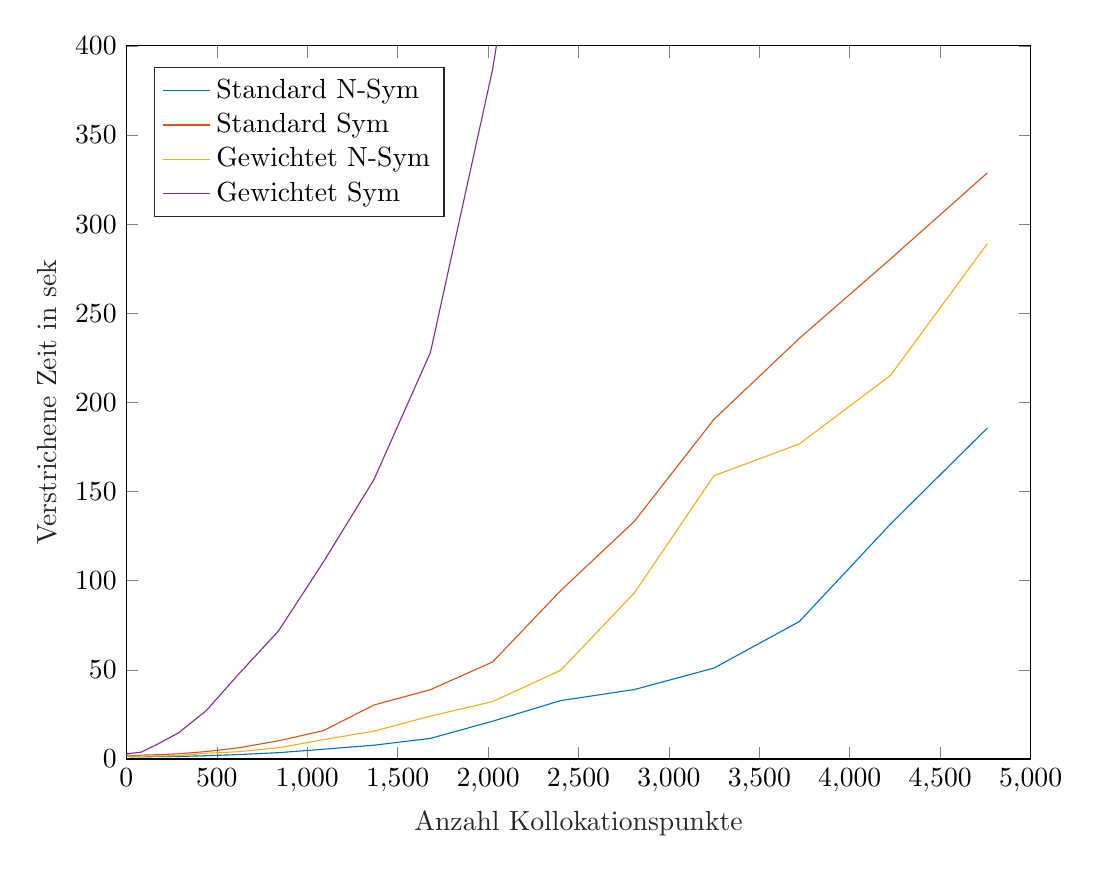
\begin{tikzpicture}

\begin{axis}[%
width=4.521in,
height=3.566in,
at={(0.758in,0.481in)},
scale only axis,
xmin=0,
xmax=5000,
xlabel style={font=\color{white!15!black}},
xlabel={Anzahl Kollokationspunkte},
ymin=0,
ymax=400,
ylabel style={font=\color{white!15!black}},
ylabel={Verstrichene Zeit in sek},
axis background/.style={fill=white},
legend style={legend cell align=left, align=left, draw=white!15!black},
legend pos = {north west}
]
\addplot [color=mycolor1]
  table[row sep=crcr]{%
3	1.90672137359608\\
25	1.24025573874677\\
81	1.2279873239107\\
169	1.31629133656873\\
289	1.40979494344081\\
441	1.83904084421868\\
625	2.49714525239894\\
841	3.55515572712825\\
1089	5.46548130424626\\
1369	7.73584542363863\\
1681	11.5576202485706\\
2025	21.1976884488541\\
2401	32.7448725596496\\
2809	38.9545642091382\\
3249	50.998666539123\\
3721	77.0899367632454\\
4225	131.742325107451\\
4761	185.639876063679\\
};
\addlegendentry{Standard N-Sym}

\addplot [color=mycolor2]
  table[row sep=crcr]{%
3	2.49451486944359\\
25	1.77853916240757\\
81	2.16015407056586\\
169	2.38334865362738\\
289	2.92048213150108\\
441	4.16884907300247\\
625	6.34703031940247\\
841	10.2044645485385\\
1089	15.8767800861084\\
1369	30.2872746038517\\
1681	38.8782330165406\\
2025	54.4223647007288\\
2401	94.4037348399908\\
2809	133.32219666331\\
3249	190.477686084096\\
3721	235.894213609101\\
4225	280.428883797178\\
4761	328.769032505983\\
};
\addlegendentry{Standard Sym}

\addplot [color=mycolor3]
  table[row sep=crcr]{%
1	2.36560557721654\\
25	1.49217104920134\\
81	1.52410267484534\\
169	1.69440098334529\\
289	1.87604848903857\\
441	3.19610578515925\\
625	4.12250761259184\\
841	6.30184537355174\\
1089	10.8405430404468\\
1369	15.6273231388717\\
1681	24.0685730613807\\
2025	32.1896716722084\\
2401	49.7327851966136\\
2809	93.1878591014658\\
3249	158.859718109327\\
3721	176.692269827122\\
4225	215.113376607861\\
4761	289.070585979693\\
};
\addlegendentry{Gewichtet N-Sym}

\addplot [color=mycolor4]
  table[row sep=crcr]{%
1	3.1783803623253\\
25	3.17594293707075\\
81	3.81476389162018\\
169	8.16417333841866\\
289	14.6948369856394\\
441	27.0932905323046\\
625	48.078742342761\\
841	71.8185277984306\\
1089	110.444175489692\\
1369	156.737761042004\\
1681	227.962964027347\\
2025	386.789968827068\\
2401	624.679365062422\\
2809	822.069315743255\\
3249	1001.81983498422\\
3721	1199.25576337967\\
4225	1614.09924184046\\
4761	1952.6937843398\\
};
\addlegendentry{Gewichtet Sym}

\end{axis}
\end{tikzpicture}%
}
\caption{Laufzeit der unterschiedlichen Verfahren}
\label{fig:Laufzeit}
\end{figure}

Wir erkennen deutliche Unterschiede zwischen den verschiedenen Verfahren. Das nicht-symmetrische Standardverfahren ist durchgehend das schnellste. Danach kommt das nicht-symmetrische gewichtete Verfahren. Der Mehraufwand entsteht hier durch den komplizierteren Kern und damit durch längere Auswertungszeiten. Mit der selben Begründung lässt sich auch die längere Laufzeit des symmetrischen Standardverfahrens erklären. Hier entstehen die komplizierteren Funktionen allerdings nicht durch das Anhängen der Gewichtsfunktion, sondern durch die zweimalige Anwendung des Differentialoperators. Beim symmetrischen gewichteten Verfahren kommen beide Effekte zusammen, was die längste Laufzeit erklärt.

In Abbildung \ref{fig:Laufzeit-greedy} ist die Laufzeit der unterschiedlichen Verfahren bei einer \\Greedy-Punktwahl dargestellt. Wieder gilt es zu beachten, dass die Graphen der Standardverfahren erst bei $37$ Kollokationspunkten beginnen.
\begin{figure}[ht]
\centering
\resizebox {.85\columnwidth} {!} {
% This file was created by matlab2tikz.
%
%The latest updates can be retrieved from
%  http://www.mathworks.com/matlabcentral/fileexchange/22022-matlab2tikz-matlab2tikz
%where you can also make suggestions and rate matlab2tikz.
%
\definecolor{mycolor1}{rgb}{0.00000,0.44700,0.74100}%
\definecolor{mycolor2}{rgb}{0.85000,0.32500,0.09800}%
\definecolor{mycolor3}{rgb}{0.92900,0.69400,0.12500}%
\definecolor{mycolor4}{rgb}{0.49400,0.18400,0.55600}%
%
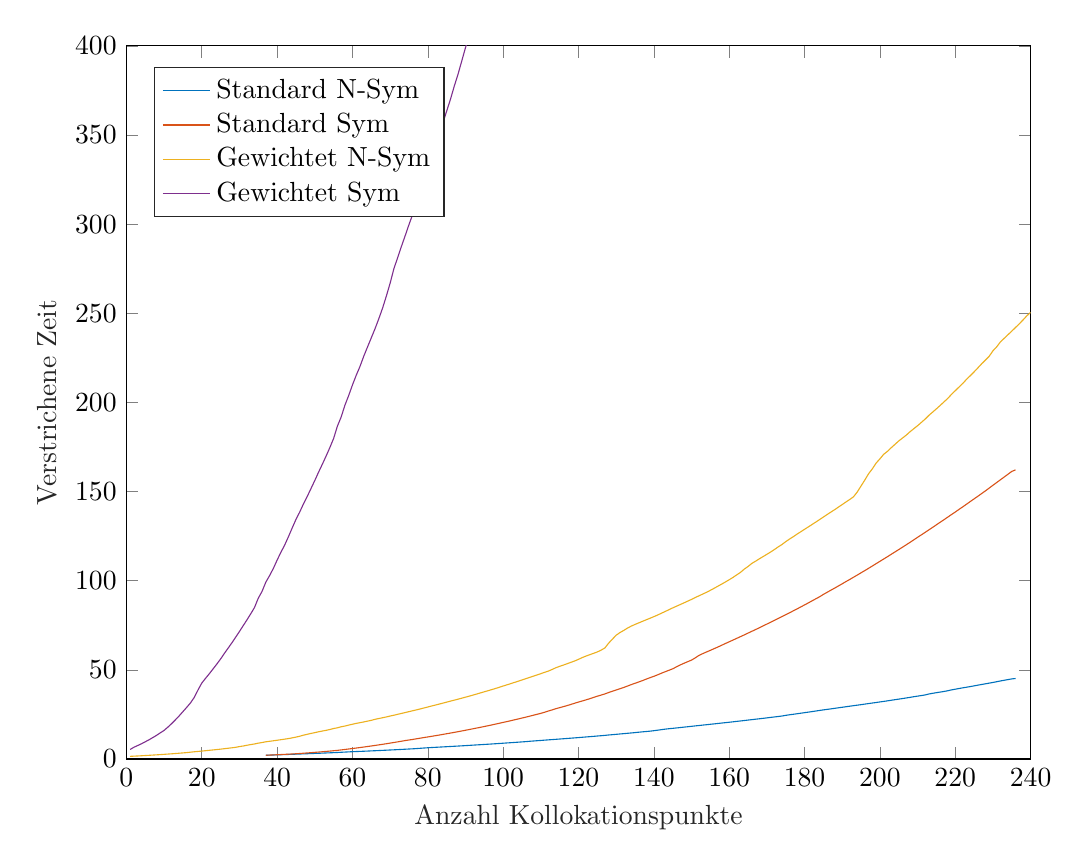
\begin{tikzpicture}

\begin{axis}[%
width=4.521in,
height=3.566in,
at={(0.758in,0.481in)},
scale only axis,
xmin=0,
xmax=240,
xlabel style={font=\color{white!15!black}},
xlabel={Anzahl Kollokationspunkte},
ymin=0,
ymax=400,
ylabel style={font=\color{white!15!black}},
ylabel={Verstrichene Zeit},
axis background/.style={fill=white},
legend style={legend cell align=left, align=left, draw=white!15!black},
legend pos = {north west}
]
\addplot [color=mycolor1]
  table[row sep=crcr]{%
37	2.08103156007943\\
38	2.16751479102886\\
39	2.24562571050515\\
40	2.33251086823986\\
41	2.40249950015745\\
42	2.46935646964591\\
43	2.54590155790763\\
44	2.62414467393638\\
45	2.71068004451986\\
46	2.80083727220214\\
47	2.87915592911801\\
48	2.95649583888771\\
49	3.03973984375353\\
50	3.1264718669725\\
51	3.20814593514076\\
52	3.29148682940528\\
53	3.38583411303298\\
54	3.47201312769243\\
55	3.55898367947345\\
56	3.66023802769312\\
57	3.76827175998361\\
58	3.87786188087777\\
59	3.99080577083112\\
60	4.0973114423506\\
61	4.18435055569765\\
62	4.26803754217871\\
63	4.35223278745463\\
64	4.44903884484846\\
65	4.54708968468659\\
66	4.6415252361987\\
67	4.74194452917705\\
68	4.84148524879432\\
69	4.94445281506811\\
70	5.05233669722925\\
71	5.15255112660612\\
72	5.25839663645989\\
73	5.3780739290745\\
74	5.48128371884503\\
75	5.60279493071382\\
76	5.71360766444409\\
77	5.84891042534035\\
78	6.00580351076273\\
79	6.16030186795371\\
80	6.30684462019561\\
81	6.43545010668098\\
82	6.54914735276404\\
83	6.66469617167816\\
84	6.78255186148757\\
85	6.89836548405492\\
86	7.01875097248628\\
87	7.13558234428827\\
88	7.25419508516209\\
89	7.38080818074964\\
90	7.5048303060186\\
91	7.64102559891812\\
92	7.76913514305761\\
93	7.90223982835797\\
94	8.03046186273153\\
95	8.15776796384876\\
96	8.29220405728462\\
97	8.42810211321526\\
98	8.56297133510718\\
99	8.71137592388763\\
100	8.85014248078737\\
101	9.00003079112247\\
102	9.14378099383069\\
103	9.28535241671309\\
104	9.4372388656222\\
105	9.58311160303921\\
106	9.73546525591323\\
107	9.93287494247192\\
108	10.0938439514124\\
109	10.2519481543185\\
110	10.4070270268051\\
111	10.5734945091218\\
112	10.7309775524506\\
113	10.8876165084756\\
114	11.0403589505893\\
115	11.2006287957756\\
116	11.3617131687883\\
117	11.5179740098293\\
118	11.6806250351532\\
119	11.8450369021339\\
120	12.0125980851206\\
121	12.186827393589\\
122	12.3596308678129\\
123	12.5277861141891\\
124	12.702105332735\\
125	12.8876563316606\\
126	13.0625609920818\\
127	13.2483624254701\\
128	13.4670237342077\\
129	13.641457085181\\
130	13.8384693609857\\
131	14.0369004917137\\
132	14.2257888377665\\
133	14.4187543389823\\
134	14.6009626536528\\
135	14.8073112083381\\
136	15.0328980563412\\
137	15.2276987084561\\
138	15.4286756491898\\
139	15.6213632092068\\
140	15.8756059179716\\
141	16.1626600573864\\
142	16.4529411064359\\
143	16.749006370478\\
144	16.9873592178562\\
145	17.1934060195413\\
146	17.4174389422305\\
147	17.6374201637513\\
148	17.8811709001723\\
149	18.0944133819039\\
150	18.3327239428073\\
151	18.5680970306273\\
152	18.788493316479\\
153	19.0177796152095\\
154	19.2392798654387\\
155	19.4673850167114\\
156	19.6980897598169\\
157	19.9212416458553\\
158	20.1591695757435\\
159	20.3861970377298\\
160	20.6214198648721\\
161	20.8535689168956\\
162	21.0992303451028\\
163	21.3349992014836\\
164	21.5805887837383\\
165	21.8277019107328\\
166	22.0727393055247\\
167	22.3173534250197\\
168	22.5556233416415\\
169	22.804888152274\\
170	23.0639379710785\\
171	23.3245195455887\\
172	23.5813482980925\\
173	23.8338552086468\\
174	24.1003745432137\\
175	24.4795122029324\\
176	24.8017256987224\\
177	25.0733900245795\\
178	25.3730709874959\\
179	25.6767026566991\\
180	25.992574823454\\
181	26.2899119661281\\
182	26.5928818314724\\
183	26.9136423968302\\
184	27.2394674860116\\
185	27.5446908509722\\
186	27.8300954073193\\
187	28.1096566297187\\
188	28.4163592002026\\
189	28.7206604736824\\
190	29.0137291456859\\
191	29.3145879716738\\
192	29.6139228423737\\
193	29.9100365511151\\
194	30.192302465712\\
195	30.4793837013146\\
196	30.7923422067874\\
197	31.1003593529266\\
198	31.3935479050336\\
199	31.6841479501118\\
200	32.0015834847914\\
201	32.2945478775269\\
202	32.6156869684169\\
203	32.9470146364574\\
204	33.266027497704\\
205	33.5833476683115\\
206	33.9038857164909\\
207	34.2296956153852\\
208	34.5737794296417\\
209	34.9363383279271\\
210	35.2629927246736\\
211	35.5869949794048\\
212	35.9178115148124\\
213	36.4556388193124\\
214	36.8458419873494\\
215	37.2026043541932\\
216	37.5340560078201\\
217	37.8857074588826\\
218	38.2704835889475\\
219	38.759313596087\\
220	39.1419959298242\\
221	39.5343672034312\\
222	39.9092064224534\\
223	40.256461722324\\
224	40.630744237852\\
225	41.0121596195367\\
226	41.4170961344004\\
227	41.7931362071988\\
228	42.1720673611228\\
229	42.5387420061114\\
230	42.9407131306073\\
231	43.3372301209434\\
232	43.7749714976843\\
233	44.1569251081897\\
234	44.541276731313\\
235	44.9202489400669\\
236	45.1485265216254\\
};
\addlegendentry{Standard N-Sym}

\addplot [color=mycolor2]
  table[row sep=crcr]{%
37	2.09977883763102\\
38	2.20546751803436\\
39	2.29646390644097\\
40	2.38746357923397\\
41	2.49892210543948\\
42	2.59771070057193\\
43	2.70770480099287\\
44	2.81912678839971\\
45	2.93914155171656\\
46	3.08307855390109\\
47	3.24313491397166\\
48	3.3945135146342\\
49	3.55213491274001\\
50	3.72088627524718\\
51	3.89433841578443\\
52	4.06684136865308\\
53	4.25632624138516\\
54	4.44166170245348\\
55	4.64287429791109\\
56	4.8428474480523\\
57	5.09336484154683\\
58	5.35242328186563\\
59	5.60770016179708\\
60	5.8700877382771\\
61	6.1441554138799\\
62	6.42501561109909\\
63	6.71256569285979\\
64	7.00355206388788\\
65	7.3047520555127\\
66	7.60768045547871\\
67	7.92233041994575\\
68	8.23855771097974\\
69	8.56945389275739\\
70	8.91083465700948\\
71	9.25577939105013\\
72	9.60640611355684\\
73	9.96774650448914\\
74	10.3402542197181\\
75	10.6589115461372\\
76	10.965049202161\\
77	11.3426111775059\\
78	11.6783358178348\\
79	12.0381526640274\\
80	12.3687204071654\\
81	12.7168382690134\\
82	13.0636904104539\\
83	13.4191152109377\\
84	13.7964727332294\\
85	14.1683638049124\\
86	14.5368633370926\\
87	14.9233822446893\\
88	15.3077925762193\\
89	15.7097037606635\\
90	16.1185339156003\\
91	16.5320135300298\\
92	16.9483604137834\\
93	17.3697582732667\\
94	17.7896490099422\\
95	18.2218931449519\\
96	18.6643229832739\\
97	19.1142354749038\\
98	19.5778820387993\\
99	20.0468283706939\\
100	20.5143221827047\\
101	20.9920382368264\\
102	21.4666283761953\\
103	21.9688118773265\\
104	22.4571845336602\\
105	22.9683056712732\\
106	23.4783930482678\\
107	23.994382467617\\
108	24.5378658960401\\
109	25.0705785898241\\
110	25.6033360333726\\
111	26.2311579884283\\
112	26.9105854541916\\
113	27.5340592922065\\
114	28.2223771813971\\
115	28.7953153975729\\
116	29.3776876031246\\
117	29.96532468007\\
118	30.6233046921155\\
119	31.2907281361477\\
120	31.9424255275648\\
121	32.538423420631\\
122	33.1693162769674\\
123	33.8262674549741\\
124	34.5531292607216\\
125	35.2224609332502\\
126	35.8538911973107\\
127	36.5086824807135\\
128	37.2821115484363\\
129	38.0124901109178\\
130	38.7125993578204\\
131	39.4115295100065\\
132	40.1176233194719\\
133	40.9066035462341\\
134	41.7283845293905\\
135	42.46385553298\\
136	43.2032563048929\\
137	43.9834241124048\\
138	44.8269448596684\\
139	45.6248126360198\\
140	46.3750863690985\\
141	47.2093734745565\\
142	48.0987405609814\\
143	48.9423902204111\\
144	49.7555303935064\\
145	50.5893823177668\\
146	51.6640598218138\\
147	52.7412449548746\\
148	53.691663857832\\
149	54.599813118414\\
150	55.4557262661002\\
151	56.7350481388409\\
152	58.1268668144367\\
153	59.118728104946\\
154	60.0478937435313\\
155	60.955028539265\\
156	61.8913988899595\\
157	62.813128677743\\
158	63.7974917141089\\
159	64.7800315054765\\
160	65.7401483803664\\
161	66.6897888837479\\
162	67.664491718625\\
163	68.6358551536333\\
164	69.6084490018955\\
165	70.6132749971569\\
166	71.6088295801692\\
167	72.5999276613896\\
168	73.6076447377766\\
169	74.6500802416652\\
170	75.6801935488903\\
171	76.7087225502275\\
172	77.7491898855679\\
173	78.8072541421244\\
174	79.8508588875701\\
175	80.9198827309837\\
176	81.9911021867034\\
177	83.0865616456746\\
178	84.1737838635633\\
179	85.3028701021075\\
180	86.4043412198293\\
181	87.540522964635\\
182	88.710950185301\\
183	89.8571862579631\\
184	90.9868796974423\\
185	92.3189061186887\\
186	93.5040855714032\\
187	94.6904346762231\\
188	95.8604743392944\\
189	97.0736006358572\\
190	98.2749388590945\\
191	99.5157586912049\\
192	100.706893147005\\
193	101.947225658283\\
194	103.178132801701\\
195	104.438473794907\\
196	105.689076582448\\
197	106.957744726815\\
198	108.248600132936\\
199	109.561203924678\\
200	110.860351585353\\
201	112.159498014383\\
202	113.45998775745\\
203	114.803402377978\\
204	116.132495431624\\
205	117.455878990068\\
206	118.80021734427\\
207	120.15203835178\\
208	121.520693071217\\
209	122.910031213987\\
210	124.317734413842\\
211	125.712865393118\\
212	127.109548244968\\
213	128.51957227436\\
214	129.92001164315\\
215	131.352068978683\\
216	132.761197602234\\
217	134.191096274808\\
218	135.658230446508\\
219	137.093441203531\\
220	138.520142936496\\
221	139.990383727179\\
222	141.432209648952\\
223	142.918461412771\\
224	144.421981248617\\
225	145.894499350718\\
226	147.366028852513\\
227	148.877334736861\\
228	150.368187515473\\
229	151.926938003512\\
230	153.51152019056\\
231	155.071634109502\\
232	156.623027572013\\
233	158.166480209314\\
234	159.723376250684\\
235	161.286418610647\\
236	162.169183669867\\
};
\addlegendentry{Standard Sym}

\addplot [color=mycolor3]
  table[row sep=crcr]{%
1	1.4921094669564\\
2	1.5946845490558\\
3	1.701274793525\\
4	1.82012318912277\\
5	1.95116569031439\\
6	2.06954318701255\\
7	2.19489713096532\\
8	2.32719878379172\\
9	2.47150363725266\\
10	2.61111920803591\\
11	2.75982965529954\\
12	2.90871951217009\\
13	3.0716977444887\\
14	3.2389850917596\\
15	3.41205213799185\\
16	3.59098797216647\\
17	3.82081660520074\\
18	4.04784817267005\\
19	4.24381108702105\\
20	4.4391524312465\\
21	4.65329072936779\\
22	4.87175210108356\\
23	5.0849867823975\\
24	5.30247474409498\\
25	5.53081021296372\\
26	5.77895012125544\\
27	6.03361364202734\\
28	6.28363016659639\\
29	6.54537646663248\\
30	6.96487348748875\\
31	7.28552156261252\\
32	7.70554203255073\\
33	8.09245383487008\\
34	8.42325107450754\\
35	8.89108810489673\\
36	9.24072130051848\\
37	9.65021982808701\\
38	9.93018831439953\\
39	10.220100691076\\
40	10.5107996782944\\
41	10.8239314351496\\
42	11.1309920037508\\
43	11.4517172619549\\
44	11.8453719095464\\
45	12.2806697028082\\
46	12.7614016447386\\
47	13.3580362982174\\
48	13.8609953250865\\
49	14.3303530263773\\
50	14.7904779069591\\
51	15.2567302209119\\
52	15.6782327702116\\
53	16.074195109795\\
54	16.5485130556412\\
55	17.0920379494426\\
56	17.4984204154174\\
57	18.0725865815573\\
58	18.4748541219255\\
59	19.0190974752511\\
60	19.4993544127989\\
61	19.961558720518\\
62	20.3740452186108\\
63	20.7867722980072\\
64	21.2322611317092\\
65	21.6821888136263\\
66	22.2584089529089\\
67	22.7016812363416\\
68	23.1437317280347\\
69	23.5800283853094\\
70	24.0974280380677\\
71	24.5555264522428\\
72	25.0595237557615\\
73	25.5524576037035\\
74	26.0568408226238\\
75	26.5563557598079\\
76	27.062647617773\\
77	27.5537508308471\\
78	28.0789804607748\\
79	28.619888930263\\
80	29.1670685250272\\
81	29.7302426709944\\
82	30.2500481367881\\
83	30.7906117457047\\
84	31.3255315471472\\
85	31.8846704138778\\
86	32.4517800758447\\
87	32.9888384233796\\
88	33.5398849725774\\
89	34.101072475323\\
90	34.6763245417152\\
91	35.2528234432932\\
92	35.8452602404089\\
93	36.4497868638503\\
94	37.079946891472\\
95	37.711687530047\\
96	38.2946624205025\\
97	38.9425031211934\\
98	39.5654916911182\\
99	40.2512284631494\\
100	40.9292526748248\\
101	41.586048255026\\
102	42.2555749379969\\
103	42.9436785209751\\
104	43.6335347346442\\
105	44.3271528023822\\
106	45.0130644679889\\
107	45.7185720144825\\
108	46.4352004933148\\
109	47.1479414902985\\
110	47.8702609896595\\
111	48.599108617532\\
112	49.3129182717395\\
113	50.2201737686733\\
114	51.1956311913249\\
115	51.9682592793153\\
116	52.696200005994\\
117	53.4522419426817\\
118	54.2227417482871\\
119	54.9999039316979\\
120	55.8925012121439\\
121	56.8987789061926\\
122	57.7402555334726\\
123	58.5084480576344\\
124	59.2692355221169\\
125	60.044719384079\\
126	61.0640796102419\\
127	62.2741547118423\\
128	64.9732540099279\\
129	67.2211496419814\\
130	69.4408381425645\\
131	70.9071976096236\\
132	72.1071288838382\\
133	73.4198135535952\\
134	74.5382152726431\\
135	75.465273977355\\
136	76.3518895690762\\
137	77.2283436798347\\
138	78.0970893357205\\
139	78.9557256502777\\
140	79.8441008520109\\
141	80.7477476293915\\
142	81.7544592729929\\
143	82.7216581060504\\
144	83.7308777892138\\
145	84.7388744489929\\
146	85.6800773637216\\
147	86.6203861042538\\
148	87.5752208647215\\
149	88.5472990643194\\
150	89.507431950593\\
151	90.573053580248\\
152	91.5519505765535\\
153	92.5350700621201\\
154	93.5166939202313\\
155	94.6110588574359\\
156	95.7480715519998\\
157	96.9190657398676\\
158	98.102174386959\\
159	99.2884335817014\\
160	100.545360865797\\
161	101.825452927148\\
162	103.283151877827\\
163	104.692305544824\\
164	106.494738618267\\
165	107.968863195864\\
166	109.687613798857\\
167	110.937111390375\\
168	112.273417367096\\
169	113.526059758589\\
170	114.799753424691\\
171	116.098222859576\\
172	117.487407046733\\
173	118.947912916137\\
174	120.279052963604\\
175	121.903414817591\\
176	123.340867989426\\
177	124.685295843157\\
178	126.110912086419\\
179	127.456555984214\\
180	128.820769802695\\
181	130.17205832906\\
182	131.524829345336\\
183	132.909349293262\\
184	134.305733676497\\
185	135.710314245985\\
186	137.120429417099\\
187	138.49331812115\\
188	139.854334589474\\
189	141.282013427393\\
190	142.716449890322\\
191	144.15860301909\\
192	145.566301702913\\
193	147.075405406182\\
194	149.783482985031\\
195	153.148331921731\\
196	156.48268286745\\
197	159.996105949379\\
198	162.744183249055\\
199	165.985790923352\\
200	168.333055665833\\
201	170.892209312303\\
202	172.551949344909\\
203	174.565079500625\\
204	176.465683704558\\
205	178.371136483908\\
206	180.013177368771\\
207	181.656327144591\\
208	183.545869124592\\
209	185.248704822752\\
210	186.945476722527\\
211	188.773032478065\\
212	190.634690838656\\
213	192.747802232315\\
214	194.543516272287\\
215	196.397446882235\\
216	198.304164560896\\
217	200.257265986443\\
218	202.217411189165\\
219	204.485682743875\\
220	206.554953737365\\
221	208.625672734707\\
222	210.639276252614\\
223	212.962128561558\\
224	214.992552243297\\
225	217.110740066681\\
226	219.341283464305\\
227	221.637902147455\\
228	223.710679633972\\
229	225.855543243668\\
230	228.922670353938\\
231	231.174603317969\\
232	233.95449852141\\
233	235.963789639978\\
234	237.972802406798\\
235	239.964780703573\\
236	242.019221460838\\
237	244.109326138338\\
238	246.259718601985\\
239	248.572970238943\\
240	250.473137208937\\
};
\addlegendentry{Gewichtet N-Sym}

\addplot [color=mycolor4]
  table[row sep=crcr]{%
1	5.34363672715822\\
2	6.59752718548203\\
3	7.56366557228175\\
4	8.5379032559354\\
5	9.65836428525389\\
6	10.7699172375683\\
7	12.01317285274\\
8	13.2572015303598\\
9	14.6660752034164\\
10	16.0342364437978\\
11	17.861061833911\\
12	19.8220843783498\\
13	21.9554809634912\\
14	24.179336529315\\
15	26.5658357305933\\
16	28.9558369088669\\
17	31.4286629221925\\
18	34.5120785362475\\
19	38.6797879271704\\
20	42.5578386602659\\
21	45.235466282284\\
22	47.8054419819301\\
23	50.516956671143\\
24	53.2398513486717\\
25	56.1034154744686\\
26	59.2012109532644\\
27	62.1718193899499\\
28	65.1626432249062\\
29	68.2803970987373\\
30	71.4927470484656\\
31	74.7801058147187\\
32	78.0419752792447\\
33	81.4277215349416\\
34	84.9732338930612\\
35	90.1671169697266\\
36	93.9843667313007\\
37	99.1541046413717\\
38	102.845384225995\\
39	106.864394665007\\
40	111.542778516993\\
41	115.886280994857\\
42	119.945487807331\\
43	124.620594252242\\
44	129.549995545551\\
45	134.343133805491\\
46	138.480806661721\\
47	143.118117209076\\
48	147.267867575183\\
49	151.712468803461\\
50	156.184034433507\\
51	160.839067940406\\
52	165.299970399468\\
53	169.877902114611\\
54	174.659377929006\\
55	179.774691093196\\
56	186.668314744391\\
57	191.786530485059\\
58	198.427336030088\\
59	203.8602678335\\
60	209.772998813105\\
61	215.206391251708\\
62	220.169560142657\\
63	225.914307895624\\
64	231.102072981529\\
65	236.224181951722\\
66	241.364688412315\\
67	246.962678285731\\
68	252.909079563029\\
69	259.659219046814\\
70	266.865848416536\\
71	275.013218423601\\
72	281.187463743453\\
73	287.493027042406\\
74	293.536305401953\\
75	299.70685086053\\
76	305.530603707169\\
77	311.621969178497\\
78	318.290612361527\\
79	324.873219811255\\
80	331.35208416897\\
81	337.714392222245\\
82	344.003278228172\\
83	350.34375209123\\
84	356.714225950183\\
85	363.340721834231\\
86	369.91226870222\\
87	377.204048252563\\
88	383.913168213544\\
89	391.390260234251\\
90	398.959095841269\\
91	405.911501797996\\
92	412.989353250947\\
93	420.307018692675\\
94	428.390501636651\\
95	436.565001906997\\
96	443.986591081988\\
97	453.251646401318\\
98	462.838411473675\\
99	470.771111112023\\
100	478.889544032742\\
101	487.807628151625\\
102	496.693985508466\\
103	504.974989808138\\
104	513.367088888223\\
105	521.826017020511\\
106	530.376054441989\\
107	539.09034361661\\
108	548.399319393029\\
109	558.142398267158\\
110	570.062414426339\\
111	588.870788133676\\
112	600.078035789138\\
113	610.696069451635\\
114	621.281430038259\\
115	632.058014990761\\
116	643.034624411941\\
117	653.983820291514\\
118	665.115988105595\\
119	676.348853153853\\
120	687.968760148241\\
121	699.856616006375\\
122	713.306796586045\\
123	725.001058804065\\
124	736.756851127386\\
125	749.168181110919\\
126	761.621019169732\\
127	773.783462047068\\
128	786.400743174532\\
129	799.619698435852\\
130	811.909433045115\\
131	825.183369345262\\
132	846.346721587081\\
133	859.987977093047\\
134	874.041513001859\\
135	888.607478876264\\
136	904.222779929279\\
137	917.597364197807\\
138	933.250917267538\\
139	946.669217540101\\
140	960.610125270603\\
141	974.695931096858\\
142	988.806976611474\\
143	1002.67144763846\\
144	1016.58847377438\\
145	1030.7111447852\\
146	1044.99215072706\\
147	1059.59822799143\\
148	1073.79714890628\\
149	1088.29064520539\\
150	1102.2121389279\\
151	1116.79841257394\\
152	1131.5713021812\\
153	1146.10046896932\\
154	1160.74771601717\\
155	1178.37107202783\\
156	1195.66282776637\\
157	1212.97695140791\\
158	1230.08908487552\\
159	1247.73555064996\\
160	1265.2176070207\\
161	1282.34576459899\\
162	1300.18971765362\\
163	1317.88254089985\\
164	1335.18673460967\\
165	1353.69056933607\\
166	1371.72839274036\\
167	1390.42806023729\\
168	1420.11820629806\\
169	1451.48855945581\\
170	1488.45870192018\\
171	1524.48402330765\\
172	1571.1992230784\\
173	1620.59609149808\\
174	1670.03165204225\\
175	1734.06094959001\\
176	1796.07986478181\\
177	1849.15851516175\\
178	1901.39281384467\\
179	1968.77127861573\\
180	2039.63416862122\\
181	2113.43868810112\\
182	2181.47568589278\\
183	2229.45887886649\\
184	2296.83181190976\\
185	2362.78551314637\\
186	2429.87218646118\\
187	2501.63444327803\\
188	2523.14283180616\\
189	2545.30238688676\\
190	2563.74875675711\\
191	2582.25025505313\\
192	2600.4918820232\\
193	2619.13986066812\\
194	2637.75480290192\\
195	2656.40210496324\\
196	2675.36666109689\\
197	2694.41872724279\\
198	2713.43598299837\\
199	2732.44147982956\\
200	2751.21891420649\\
201	2770.60928077275\\
202	2790.06080548755\\
203	2809.64280819964\\
204	2829.21046922797\\
205	2848.60295176016\\
206	2868.44426539977\\
207	2888.04733006072\\
208	2907.28044308015\\
209	2927.14896991379\\
210	2946.90126929218\\
211	2966.33914368657\\
212	2987.78677435075\\
213	3008.09507190138\\
214	3028.1595312688\\
215	3048.40971817091\\
216	3068.83293845429\\
217	3089.34285996978\\
218	3109.77561482687\\
219	3130.06406318831\\
220	3149.86043164227\\
221	3169.96139162736\\
222	3190.88297731269\\
223	3211.87887757737\\
224	3232.8150459383\\
225	3253.30512770721\\
226	3273.81868627007\\
227	3294.24203916056\\
228	3315.09977021612\\
229	3335.978052909\\
230	3356.93184980337\\
231	3378.07404402802\\
232	3399.07103101405\\
233	3419.92236038997\\
234	3441.18661965615\\
235	3462.52845079189\\
236	3484.17266635109\\
237	3505.88449757304\\
238	3527.74085534454\\
239	3549.68001619203\\
240	3566.79219153556\\
};
\addlegendentry{Gewichtet Sym}

\end{axis}
\end{tikzpicture}%
}
\caption{Laufzeit bei Greedy-Punktwahl}
\label{fig:Laufzeit-greedy}
\end{figure}

Wir erhalten wieder die gleiche Reihenfolge der Verfahren, die wir genauso begründen können, wie schon im Fall der auf einem Gitter verteilten Punkte. Allerdings benötigt das Greedy-Verfahren wesentlich mehr Zeit für gleich viele Punkte. Das liegt daran, dass beim Greedy-Verfahren alle vorhergegangenen Iterationen zur Punktwahl mitberechnet werden müssen, was im Falle des Gitters wegfällt.

\section{Vergleich mit der finiten Elemente Methode}
Die Kernkollokation bietet einige Vorteile gegenüber der \ac{FEM}. Zunächst kann jene auch für höhere Dimensionen eingesetzt werden, wie wir in Kapitel \ref{sec:4D} beispielhaft in vier Dimensionen gesehen haben, wobei die \ac{FEM} nur für bis zu drei Dimensionen eingesetzt wird.

Außerdem hat die Kernkollokation eine höhere Genauigkeit als die \ac{FEM}. In der folgenden Tabelle \ref{tab:FEM} ist der Fehler der \ac{FEM} und der Kernkollokation mit zufälligen Kollokationspunkten für die erste \ac{PDE} dargestellt. $n$ bezeichnet dabei die Knotenanzahl, beziehungsweise die Anzahl der Kollokationspunkte. Wir sehen, dass selbst die gewichteten Kollokationsverfahren, die in diesem Fall vergleichsweise schlecht abgeschnitten haben, einen geringeren Fehler als die \ac{FEM} haben.
\begin{table}[ht]
\centering
\begin{tabular}{c|ccc}
 & $n=183$ & $n=689$ & $n=2673$ \\ 
\hline 
FEM & \num{3.3902e-02} & \num{1.1434e-02} & \num{3.6496e-03} \\ 
Standard N-Sym & \num{6.3587e-03} & \num{9.1230e-05} & \num{1.6121e-05} \\ 
Standard Sym & \num{3.9065e-03} & \num{1.0242e-05} & \num{3.2350e-07} \\ 
Gewichtet N-Sym & \num{5.8360e-03} & \num{3.1449e-03} & \num{3.0448e-04} \\ 
Gewichtet Sym & \num{9.9156e-03} & \num{1.0253e-03} & \num{4.0773e-04} \\ 
\end{tabular}
\caption{Vergleich \acs{FEM} mit Kernkollokation}
\label{tab:FEM}
\end{table}